\documentclass[10pt,a4paper]{article}
\usepackage[margin=1.7cm]{geometry}
\usepackage{amsmath}
\usepackage{tikz}
\usetikzlibrary{arrows.meta,positioning,shapes.geometric,fit,calc}
\usepackage[most]{tcolorbox}
\usepackage{booktabs,tabularx}
\usepackage{enumitem}
\usepackage{titlesec}
\usepackage{xcolor}
\usepackage{colortbl}
\usepackage[hidelinks]{hyperref}
\setlist{nosep,leftmargin=1.2em}
\setlength{\parindent}{0pt}
\setlength{\parskip}{3pt}
\setlength{\emergencystretch}{3em}
\titlespacing*{\section}{0pt}{8pt}{4pt}
\titlespacing*{\subsection}{0pt}{6pt}{2pt}

% ---------- Atom One Light theme ----------
\makeatletter
\def\XC@clr@rgb@white{0.98039,0.98039,0.98039}% #FAFAFA
\def\XC@clr@gray@white{0.98}
\makeatother
\definecolor{white}{HTML}{FAFAFA}   % background
\definecolor{black}{HTML}{383A42}   % foreground
\definecolor{red}{HTML}{E45649}
\definecolor{orange}{HTML}{986801}
\definecolor{yellow}{HTML}{C18401}
\definecolor{green}{HTML}{50A14F}
\definecolor{cyan}{HTML}{0184BC}
\definecolor{blue}{HTML}{4078F2}
\definecolor{magenta}{HTML}{A626A4}
\definecolor{brown}{HTML}{986801}
\definecolor{gray}{HTML}{A0A1A7}
\definecolor{acc}{HTML}{4078F2}     % blue: headings, key boxes
\definecolor{warn}{HTML}{E45649}    % red: exam tips, highlights
\definecolor{ok}{HTML}{50A14F}      % green
\pagecolor{white}
\AtBeginDocument{\color{black}\def\normalcolor{\color{black}}}
\tcbset{colupper=black,collower=black,coltitle=white}% tcolorbox froze the old black/white at load time
% code font
\usepackage{fontspec}
% text: Fira Sans (pairs with Fira Math); code: AnnotationM
\setmainfont{FiraSans}[Extension=.otf,UprightFont=*-Regular,BoldFont=*-SemiBold,ItalicFont=*-Italic,BoldItalicFont=*-SemiBoldItalic]
\setsansfont{FiraSans}[Extension=.otf,UprightFont=*-Regular,BoldFont=*-SemiBold,ItalicFont=*-Italic,BoldItalicFont=*-SemiBoldItalic]
\IfFontExistsTF{AnnotationM Nerd Font Mono}{\setmonofont{AnnotationM Nerd Font Mono}[Scale=MatchLowercase]}%
  {\setmonofont{FiraMono}[Extension=.otf,UprightFont=*-Regular,BoldFont=*-Bold,Scale=MatchLowercase]}% fallback (cloud build)
\usepackage{unicode-math}
\setmathfont{FiraMath-Regular.otf}[Scale=0.95]
% glyphs missing from AnnotationM and Fira Math: take them from STIX Two
\newfontfamily\symfallback{STIXTwoMath-Regular.otf}
\AtBeginDocument{\renewcommand{\checkmark}{\text{\symfallback\char"2713}}\renewcommand{\bigstar}{\text{\symfallback\char"2605}}}
\titleformat{\section}{\large\bfseries\color{acc}}{\thesection}{0.6em}{}
\titleformat{\subsection}{\normalsize\bfseries}{\thesubsection}{0.5em}{}

\newtcolorbox{keybox}[1][]{colback=acc!6,colframe=acc,boxrule=0.6pt,arc=2pt,left=4pt,right=4pt,top=2pt,bottom=2pt,fonttitle=\bfseries\small,#1}
\newtcolorbox{examtip}{colback=warn!6,colframe=warn,boxrule=0.6pt,arc=2pt,left=4pt,right=4pt,top=2pt,bottom=2pt,title=Exam tips,fonttitle=\bfseries\small}
\newtcolorbox{trap}[1][]{colback=warn!6,colframe=warn,boxrule=0.6pt,arc=2pt,left=4pt,right=4pt,top=2pt,bottom=2pt,title={Trap#1},fonttitle=\bfseries\small}
\newtcolorbox{fixbox}{colback=gray!6,colframe=gray!60,boxrule=0.6pt,arc=2pt,left=4pt,right=4pt,top=2pt,bottom=2pt,title=Corrections to the notes / slides,fonttitle=\bfseries\small,coltitle=black}

\tikzset{
  box/.style={draw,rounded corners=2pt,align=center,font=\small,minimum height=7mm,inner sep=3pt},
  circ/.style={draw,circle,fill=orange!25,font=\small\bfseries,minimum size=8mm},
  arr/.style={-{Stealth[length=2mm]},thick},
  darr/.style={{Stealth[length=2mm]}-{Stealth[length=2mm]},thick}
}
\usepackage{soul}
\let\soulhl\hl
\renewcommand{\hl}[1]{\cellcolor{warn!18}\textbf{#1}}% table-cell highlight (kept for old sections)
\sethlcolor{yellow!30}
\newcommand{\imp}[1]{\soulhl{#1}}% highlight = write this in the exam
\newcommand{\ttx}[1]{\texttt{#1}}

\usepackage[normalem]{ulem}
\newcommand{\pfcell}[3]{\fill[#3] (#1-1,1-#2) rectangle (#1,-#2);}
\newcommand{\pfletters}[1]{%
  \foreach \row [count=\r] in #1{\foreach \l [count=\c] in \row {\node[font=\small] at (\c-0.5,0.5-\r) {\l};}}
  \foreach \i in {0,...,5}{\draw[gray!70] (\i,0) -- (\i,-5); \draw[gray!70] (0,-\i) -- (5,-\i);}}
\newcommand{\MONARCHY}{{M,O,N,A,R},{C,H,Y,B,D},{E,F,G,{I/J},K},{L,P,Q,S,T},{U,V,W,X,Z}}
\setcounter{tocdepth}{2}
\setlength{\headheight}{14pt}

% ---------- importance markers (same system as the DBMS / CN / ES notes) ----------
\definecolor{gold}{HTML}{C18401}
\definecolor{good}{HTML}{50A14F}
\definecolor{trick}{HTML}{A626A4}
\newcommand{\hot}{\texorpdfstring{\textcolor{gold}{$\bigstar$}}{\9042\005}}% high-priority topic
\newcommand{\hothot}{\texorpdfstring{\textcolor{gold}{$\bigstar\bigstar$}}{\9042\005\9042\005}}% asked in BOTH past papers
\newcommand{\asked}[1]{\par\noindent{\small\textcolor{gold}{\textbf{$\bigstar$ In the papers:}} #1}\par}
\newcommand{\new}{\texorpdfstring{\textcolor{acc}{$\blacktriangleright$}}{\9045\266}}% new-in-syllabus marker for headings
\newcommand{\likely}[1]{\par\noindent{\small\textcolor{acc}{\textbf{$\blacktriangleright$ Likely this year:}} #1}\par}
\newtcolorbox{mustknow}[1][]{colback=yellow!10,colframe=gold,boxrule=0.9pt,arc=2pt,left=4pt,right=4pt,top=2pt,bottom=2pt,title={$\bigstar$ MUST KNOW #1},fonttitle=\bfseries\small,breakable}
\newtcolorbox{intuition}[1][]{colback=good!6,colframe=good,boxrule=0.6pt,arc=2pt,left=4pt,right=4pt,top=2pt,bottom=2pt,title={THE IDEA #1},fonttitle=\bfseries\small,breakable}
\newtcolorbox{worked}[1][]{colback=white,colframe=acc!70,boxrule=0.6pt,arc=2pt,left=4pt,right=4pt,top=2pt,bottom=2pt,title={WORKED EXAMPLE #1},fonttitle=\bfseries\small,breakable}
\newtcolorbox{mnemonic}[1][]{colback=trick!6,colframe=trick,boxrule=0.6pt,arc=2pt,left=4pt,right=4pt,top=2pt,bottom=2pt,title={MEMORY TRICK #1},fonttitle=\bfseries\small}

\hypersetup{bookmarksdepth=1}


\begin{document}

\begin{center}
{\LARGE\bfseries Cryptography \& Network Security}\\[2pt]
{\large Mid-Sem Notes: Lectures 1--14 (up to Message Integrity)}
\end{center}
\begin{center}\small
\begin{tabular}{@{}lll@{}}
\hothot\ = asked in \emph{both} past papers & \hot\ = asked once / high priority & \textcolor{acc}{$\blacktriangleright$} = new in this year's syllabus, likely\\[3pt]
\fcolorbox{gold}{yellow!10}{\strut\textbf{$\bigstar$ MUST KNOW}} & \fcolorbox{warn}{warn!6}{\strut\textbf{TRAP}} & \imp{highlight = write this in the exam}
\end{tabular}
\end{center}
{\small\tableofcontents}

% Priority map: what the two past mid-sem papers asked, what is new this year, and the order to study in.
\section{What to Study First}\label{sec:roadmap}

\subsection{What the paper looks like}
The mid-sem (CSN15403) is 90 minutes for 25 marks, with five to seven questions and the instruction that only a ``precise answer with proper justification'' gets full marks. In practice this means that every numerical must show its working in the textbook layout: the extended-Euclid table with its $q, r_1, r_2, r, t_1, t_2, t$ columns, the Playfair digrams, the long divisions of polynomials, and a final check. The questions are not written from the slides. They are taken almost word for word from \textbf{Forouzan} (Eve and Alice, $\mathbb{Z}_{100}$, keyed transposition, GF$(2^8)$) and \textbf{Stallings} (the ``sendmoremoney'' one-time pad, the AES state values), so the notes teach the textbook method wherever the slides are thin.

\subsection{What the two past papers asked}
Both papers are solved in full in \S\ref{sec:pastpapers}. The table lists every question by topic, with its marks.
\begin{center}\small
\begin{tabularx}{\textwidth}{@{}l X c c l@{}}
\toprule
 & Topic & 2024--25 & 2025--26 & Where\\
\midrule
\hothot & Playfair encryption & 3 & 4 & \S\ref{sec:playfair}\\
\hothot & GF$(2^8)$ inverse by the extended Euclidean algorithm & 4 & 4 & \S\ref{sec:algebra}\\
\hothot & Extended Euclid: integer inverse (``value in iteration $k$''), Diophantine equation & 5 & 3 & \S\ref{sec:exteuclid}\\
\hot & One-time-pad version of Vigen\`ere (encrypt, then find a key) & -- & 8 & \S\ref{sec:poly}, \S\ref{sec:otp}\\
\hot & AES: ShiftRows and AddRoundKey on a given state & -- & 6 & \S\ref{sec:aes}\\
\hot & DES: Feistel structure, round function, key generation, pseudocode & 5 & -- & \S\ref{sec:des}\\
\hot & GF$(p)$ division, Fermat exponent reduction, inverse that does not exist & 3 & -- & \S\ref{sec:fermat}\\
\hot & Keyed transposition and the attack type & 3 & -- & \S\ref{sec:classextra}, \S\ref{sec:attacks}\\
\hot & Characters changed: multiplicative, affine, Vigen\`ere, auto-key & 2 & -- & \S\ref{sec:classextra}\\
\midrule
\new & Lectures 10--14: primality, CRT, RSA, ElGamal, ECC, hashing & -- & -- & \S\ref{sec:primes}--\S\ref{sec:integrity}\\
\bottomrule
\end{tabularx}
\end{center}
Three patterns stand out. First, classical ciphers carried 20 of the 50 marks, and Playfair appeared in both years, so it is the safest marks in the paper. Second, the extended Euclidean algorithm appeared in both years twice over: once with integers (an inverse or a Diophantine equation) and once with polynomials (the GF$(2^8)$ inverse). Together these were 16 of the 50 marks, all from one table method. Third, each year had one block-cipher question worth 5--6 marks, DES in one year and AES in the other.

\subsection{What is new this year \new}
Neither paper asked anything from Lectures 10--14, most likely because those lectures came after the mid-sem in earlier years. This year the syllabus runs up to ``Message Integrity'', so you should expect at least one question from these lectures. The most likely is an RSA numerical in Forouzan's style: given $p$, $q$ and $e$, find $d$ with the extended-Euclid table, then encrypt and decrypt using square-and-multiply. This combines three topics you already need anyway. The next most likely are a CRT system, a Miller--Rabin test, an ElGamal or elliptic-curve computation, and a theory question on hash functions (the three resistance properties, or the birthday attack). This is a prediction from the syllabus, not from a paper, so the chapters marked \new teach these topics fully rather than as summaries.

\subsection{Priority and study order}
The order below puts the highest marks per hour first. Each step names the chapters to read and the exercise that proves you have learned it.
\begin{enumerate}[leftmargin=1.6em,itemsep=2pt]
\item \hothot\ \textbf{Extended Euclid} (\S\ref{sec:exteuclid}). Reproduce the $23^{-1} \bmod 100$ table and the $19x + 13y = 20$ solution without looking. Everything in steps 2, 5 and 6 reuses this table.
\item \hothot\ \textbf{GF$(2^8)$ inverse} (\S\ref{sec:algebra}). Learn polynomial long division over GF(2), then redo the $x^5$ and $x^7$ inverses from the papers.
\item \hothot\ \textbf{Playfair} (\S\ref{sec:playfair}), then \hot\ \textbf{Vigen\`ere, auto-key and the one-time pad} (\S\ref{sec:poly}, \S\ref{sec:otp}), then multiplicative/affine, keyed transposition and the attack types (\S\ref{sec:classextra}, \S\ref{sec:attacks}). These are mechanical and fast to practise.
\item \hot\ \textbf{AES and DES} (\S\ref{sec:modern}--\S\ref{sec:aes}). Be able to draw the DES round and key schedule, and to do ShiftRows, AddRoundKey, an S-box lookup and one MixColumns column by hand.
\item \hot\ \textbf{Modular exponentiation, Fermat and Euler} (\S\ref{sec:modexp}, \S\ref{sec:totient}, \S\ref{sec:fermat}). Exponent reduction, inverses, and ``the inverse does not exist'' traps.
\item \new\ \textbf{RSA} (\S\ref{sec:rsa}), then \textbf{CRT, Miller--Rabin and discrete logs} (\S\ref{sec:primes}), then \textbf{ElGamal and ECC} (\S\ref{sec:elgamal}), then \textbf{hash functions} (\S\ref{sec:integrity}).
\item Finally, the drill bank (\S\ref{sec:drill}) and the timed mock paper in \S\ref{sec:pastpapers}.
\end{enumerate}
Topics without a marker (the security model, Caesar and monoalphabetic ciphers, Hill, steganography, the GCD chapter) are worth one read for the theory questions, but they did not earn marks in either paper.

% Sources: Neso videos (model for network security, network access security model, symmetric cipher model, types of
% cryptography, security of encryption schemes; crypto/notes1.md), slides L1 (definitions), Stallings ch. 1--2,
% Forouzan ch. 1 and 3. Brute-force times recomputed by script (scratchpad/r1/verify.py).
\section{Model for Network Security}\label{sec:netmodel}

Two parties, a sender $S$ and a receiver $R$, want to exchange messages over an insecure communication facility such as the Internet. The parties are called \textbf{principals}. Computer networking is concerned with getting the message from $S$ to $R$; network security is concerned with what can go wrong on the way, because the path passes through links and routers that neither principal controls. Anyone with access to the path, called the \textbf{opponent} (eavesdropper, sniffer, attacker), can read, copy, change or block what is sent. The model below shows the general pattern that every protection scheme in this course follows.

\begin{center}
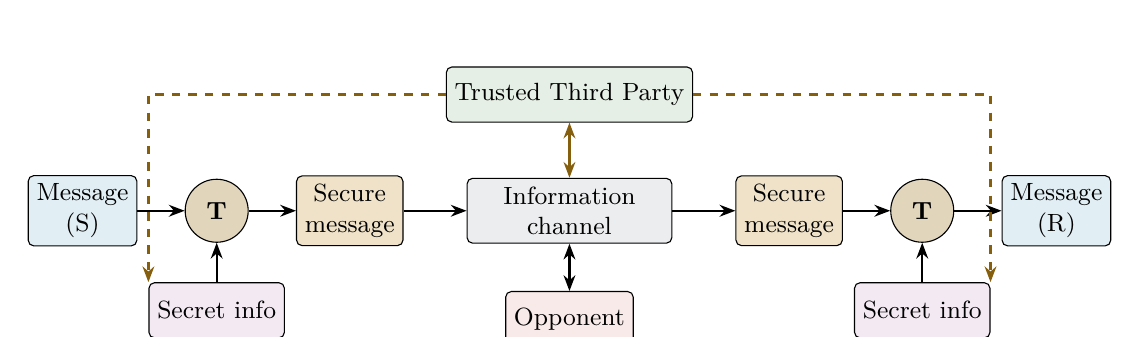
\begin{tikzpicture}[node distance=6mm]
  \node[box,fill=cyan!10] (m1) {Message\\(S)};
  \node[circ,right=of m1] (t1) {T};
  \node[box,below=5mm of t1,fill=magenta!8] (k1) {Secret info};
  \node[box,right=of t1,fill=yellow!20] (c1) {Secure\\message};
  \node[box,right=8mm of c1,minimum width=26mm,fill=gray!15] (ch) {Information\\channel};
  \node[box,right=8mm of ch,fill=yellow!20] (c2) {Secure\\message};
  \node[circ,right=of c2] (t2) {T};
  \node[box,below=5mm of t2,fill=magenta!8] (k2) {Secret info};
  \node[box,right=of t2,fill=cyan!10] (m2) {Message\\(R)};
  \node[box,below=6mm of ch,fill=red!10] (op) {Opponent};
  \node[box,above=7mm of ch,fill=green!12] (ttp) {Trusted Third Party};
  \draw[arr] (m1)--(t1); \draw[arr] (k1)--(t1); \draw[arr] (t1)--(c1);
  \draw[arr] (c1)--(ch); \draw[arr] (ch)--(c2);
  \draw[arr] (c2)--(t2); \draw[arr] (k2)--(t2); \draw[arr] (t2)--(m2);
  \draw[darr] (op)--(ch);
  \draw[darr,orange!80!black] (ttp)--(ch);
  \draw[arr,orange!80!black,dashed] (ttp.west) -| (k1.north west);
  \draw[arr,orange!80!black,dashed] (ttp.east) -| (k2.north east);
\end{tikzpicture}
\end{center}

\textbf{The transformation and the secret.} Instead of sending the plaintext message, $S$ passes it through a \textbf{security-related transformation} $T$. The transformation has two inputs: the message and a piece of \textbf{secret information} (normally a \textbf{key}, a string of bits that selects one particular transformation out of a whole family). Its output is the \textbf{secure message}, for example a ciphertext. At the other end $R$ applies the complementary transformation with its own copy of the secret information and gets the original message back. Stallings sums up the model in one sentence: \imp{every technique for providing security has two components, a security-related transformation of the information to be sent and some secret information shared by the two principals.}

\textbf{Why $T$ and not $E$.} The box is labelled $T$ rather than $E$ (encryption) because encryption is only one kind of transformation. \textbf{Steganography}, which hides the message inside an innocent-looking carrier such as an image or an audio file so that its very existence is concealed, is another; appending an authentication code or a signature to the message is a third. The model covers all of them.

\textbf{What the opponent can do.} The opponent sits on the channel and can intercept the secure message, but since it was transformed with a secret he does not have, he cannot recover the content. Security therefore does \emph{not} come from hiding how $T$ works: the algorithms are public and standardised. It comes from two things: the strength of the algorithm, and the secrecy and length of the key. If the key can take only a few values, the opponent simply tries all of them (a brute-force attack, \S\ref{sec:bruteforce}); every extra key bit doubles his work.

\textbf{The trusted third party.} A \textbf{trusted third party} (TTP) is an entity that both principals trust and that the opponent cannot impersonate. It may be needed to \emph{distribute} the secret information to $S$ and $R$ while keeping it from the opponent (a key distribution centre), to \emph{certify} public keys, or to \emph{arbitrate} disputes between the principals about whether a message was really sent or received. A familiar example is the certificate authority (CA) that signs a bank's SSL/TLS certificate: when a customer opens the bank's website, the browser trusts the bank's public key only because a CA it already trusts vouches for it. The details come in key management (\S\ref{sec:keymgmt}).

\subsection{Four tasks in designing a security service}
Each component of the model turns into one design task. A transformation is needed, so an algorithm must be designed; the algorithm needs secret information, so keys must be generated; both principals need the same (or matching) secret information, so it must be distributed; and the principals must use all of this in the same way, so a protocol must be fixed.

\begin{mustknow}[: the four tasks (Stallings)]
\begin{enumerate}[leftmargin=1.5em]
  \item \textbf{Design an algorithm} for performing the security-related transformation (encryption at $S$, decryption at $R$), such that an opponent cannot defeat its purpose.
  \item \textbf{Generate the secret information} to be used with the algorithm: keys large and random enough that guessing or exhaustive search is infeasible.
  \item \textbf{Develop methods for the distribution and sharing} of the secret information, so that $S$ and $R$ obtain it without the opponent learning it.
  \item \textbf{Specify a protocol} to be used by the two principals that makes use of the algorithm and the secret information to achieve a particular security service (e.g.\ SSL/TLS, IPsec).
\end{enumerate}
Memory aid: \emph{Algorithm $\to$ Key $\to$ Distribute $\to$ Protocol}.
\end{mustknow}

Task 1 is where cryptographic design happens (the ciphers of the coming chapters). Task 2 is harder than it looks, because a key produced by a predictable process (a timestamp, a weak random-number generator) shrinks the effective key space no matter how long the key is. Task 3 is the \emph{key distribution problem}: in symmetric cryptography both principals need the same key, and sending it over the channel it is meant to protect defeats the purpose; it is solved by a TTP, by public-key methods or by Diffie--Hellman. Task 4 exists because a strong algorithm with good keys can still be used insecurely: the protocol fixes the message formats, the order of messages and the checks each party performs, which is what SSL/TLS and IPsec standardise.

\section{Network Access Security Model}\label{sec:accessmodel}

The first model protects a \emph{message in transit}. A second class of threats targets an \emph{information system} itself: an opponent tries to get into a computer system through the network, to read or change the data stored there or to disrupt its service. Stallings divides such threats into \textbf{information access threats}, which intercept or modify data on behalf of users who should not have access to it, and \textbf{service threats}, which exploit flaws in services to stop legitimate users from using them.

\begin{center}
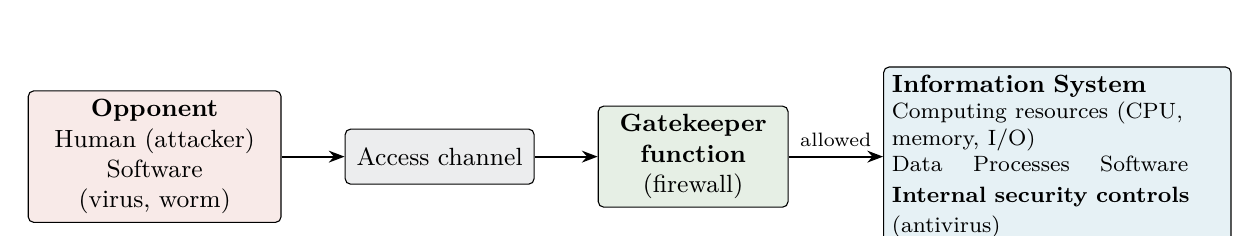
\begin{tikzpicture}[node distance=8mm]
  \node[box,fill=red!10,text width=30mm] (op) {\textbf{Opponent}\\Human (attacker)\\Software (virus, worm)};
  \node[box,right=of op,fill=gray!15,minimum width=24mm] (ac) {Access channel};
  \node[box,right=of ac,fill=green!12,text width=22mm] (gk) {\textbf{Gatekeeper function}\\(firewall)};
  \node[box,right=12mm of gk,fill=cyan!8,text width=42mm,align=left] (is) {\textbf{Information System}\\
    \footnotesize Computing resources (CPU, memory, I/O)\\ \footnotesize Data \quad Processes \quad Software\\
    \footnotesize\textbf{Internal security controls} (antivirus)};
  \draw[arr] (op)--(ac); \draw[arr] (ac)--(gk); \draw[arr] (gk)--node[above,font=\scriptsize]{allowed} (is);
\end{tikzpicture}
\end{center}

The \textbf{opponent} may be a human (a hacker who breaks in for the challenge, a criminal after money, a disgruntled ex-employee) or software (viruses, worms, Trojan horses), which may arrive over the network or on a USB stick. It reaches the system through the \textbf{access channel}, normally the Internet. The \textbf{information system} contains the assets to be protected: computing resources (processor, memory, I/O), data, running processes and installed software.

Defence is placed in two layers. The \textbf{gatekeeper function} is the first line, like a guard at a gate: it examines everything that comes in through the access channel and admits only what is allowed. Firewalls, packet filters, password-based login procedures and screening logic that rejects worms and viruses all belong here. Since no gate is perfect and some attacks start inside, the second line consists of \textbf{internal security controls}, which run inside the system and watch its activity and stored information to detect and contain whatever got past the gate: antivirus software, file-integrity checkers, intrusion detection and operating-system access permissions.

\textbf{Insiders.} An employee who misuses legitimate access never passes the gatekeeper, so only the internal controls can catch him. Insider attacks can do great damage, but the model is drawn mainly for the outside opponent, who must come through the access channel.

\begin{center}\small
\begin{tabularx}{\textwidth}{@{}l X X@{}}
\toprule
 & Model for network security & Network access security model\\
\midrule
Protects & a message while it travels from $S$ to $R$ & an information system and the resources inside it\\
Opponent & on the channel, between the principals & outside the system, trying to get in (or an insider)\\
Defence & security-related transformation with secret information (encryption, MAC, signature) & gatekeeper (firewall, login) plus internal security controls (antivirus, IDS)\\
Extra party & trusted third party for keys and disputes & none required\\
\bottomrule
\end{tabularx}
\end{center}

\section{Cryptography}\label{sec:cryptobasics}

The Concise Oxford English Dictionary defines cryptography as ``the art of writing or solving codes''. The definition used in this course (Stallings, quoted in the lecture) is more precise:
\begin{center}
\imp{Cryptography is the art or science encompassing the principles and methods of transforming an intelligible}\\
\imp{message into one that is unintelligible, and then retransforming that message back to its original form.}
\end{center}
\textbf{Intelligible} means readable by anyone; \textbf{unintelligible} means meaningless to anyone who does not hold the key; \textbf{retransforming} means the process must be reversible by the intended receiver. The word ``art'' reflects that classical ciphers were designed by ingenuity; modern cryptography is a science built on mathematics and complexity theory.

\textbf{Terminology.} The original message is the \textbf{plaintext} (clear text) and the coded message is the \textbf{ciphertext}. Converting plaintext to ciphertext is \textbf{enciphering} or \textbf{encryption}; recovering the plaintext is \textbf{deciphering} or \textbf{decryption}. The scheme used is a \textbf{cryptographic system} or \textbf{cipher}, and the \textbf{key} is the input to the cryptographic algorithm that selects the particular transformation. The slides contrast \textbf{cryptography}, the science of creating coded messages, with \textbf{cryptanalysis}, the art of breaking them, i.e.\ recovering the plaintext or the key without being told the key. The two together form \textbf{cryptology}.

\textbf{Scope today.} Cryptography now covers much more than secret writing: mechanisms for ensuring integrity, techniques for exchanging secret keys, protocols for authenticating users, electronic auctions and elections, and digital cash. Forouzan groups the tools into three mechanisms: \textbf{symmetric-key encipherment}, \textbf{asymmetric-key encipherment} and \textbf{hashing}.

\subsection{Symmetric cipher model}
A symmetric (conventional, single-key) cipher has five ingredients (Stallings): the \textbf{plaintext}; the \textbf{encryption algorithm}, which performs substitutions and transformations on the plaintext; the \textbf{secret key}, also an input to the encryption algorithm, which determines the exact substitutions and transformations; the \textbf{ciphertext}, which depends on both the plaintext and the key, so that two different keys give two different ciphertexts for the same message; and the \textbf{decryption algorithm}, which is the encryption algorithm run in reverse with the same key.

\begin{center}
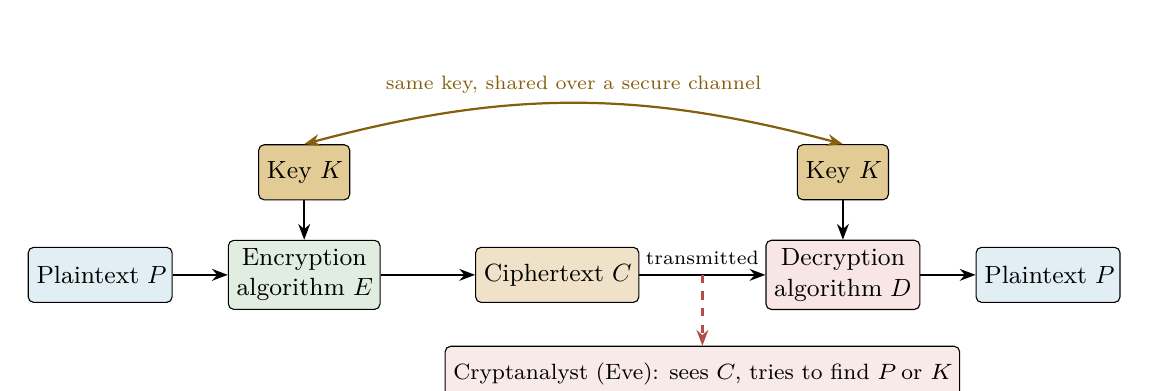
\begin{tikzpicture}[node distance=7mm]
  \node[box,fill=cyan!10] (p1) {Plaintext $P$};
  \node[box,right=of p1,fill=green!15] (e) {Encryption\\algorithm $E$};
  \node[box,right=12mm of e,fill=yellow!20] (c) {Ciphertext $C$};
  \node[box,right=16mm of c,fill=red!12] (d) {Decryption\\algorithm $D$};
  \node[box,right=of d,fill=cyan!10] (p2) {Plaintext $P$};
  \node[box,above=5mm of e,fill=yellow!40] (k1) {Key $K$};
  \node[box,above=5mm of d,fill=yellow!40] (k2) {Key $K$};
  \draw[arr] (p1)--(e); \draw[arr] (k1)--(e); \draw[arr] (e)--(c);
  \draw[arr] (c)--node[above,font=\scriptsize]{transmitted}(d); \draw[arr] (k2)--(d); \draw[arr] (d)--(p2);
  \draw[darr,bend left=15,orange!80!black] (k1.north) to node[above,font=\scriptsize]{same key, shared over a secure channel} (k2.north);
  \coordinate (mid) at ($(c.east)!0.5!(d.west)$);
  \node[box,below=9mm of mid,fill=red!10,font=\footnotesize] (eve) {Cryptanalyst (Eve): sees $C$, tries to find $P$ or $K$};
  \draw[arr,dashed,red!70!black] (mid) -- (eve.north);
\end{tikzpicture}
\end{center}
\[
C = E(K, P) \qquad\qquad P = D(K, C) = D\big(K, E(K,P)\big)
\]
Both algorithms take \textbf{two} inputs: encryption takes $P$ and $K$, decryption takes $C$ and $K$. The equation on the right is the correctness requirement: $D$ with key $K$ must be the inverse of $E$ with key $K$, so that applying one after the other returns the original input.

\textbf{Requirements for secure use.} Stallings states two. First, the encryption algorithm must be strong: an opponent who knows the algorithm and holds many ciphertexts, even together with their plaintexts, must be unable to decrypt other ciphertexts or to find the key. Second, sender and receiver must have obtained their copies of the key in a secure fashion and must keep it secure. The algorithms $E$ and $D$ are \textbf{public}; only $K$ is secret (Kerckhoff's principle, \S\ref{sec:attacks}). This is what makes symmetric encryption practical: since the algorithm need not be hidden, manufacturers can build cheap chips implementing it, and the only thing that must be protected is the key.

\textbf{The key is everything.} If the opponent recovers one plaintext, he has read one message. If he recovers the key, he can read \emph{every} past and future message encrypted under it, which is why cryptanalysts aim at the key. In the lecture's toy example both ends use $K = 100$; such a key would be found instantly. Real symmetric keys are 128 or 256 bits long (2048 bits is the size of an RSA modulus, a different kind of key), so exhaustive search is out of reach (\S\ref{sec:schemes}).

\subsection{Types of cryptography}
Cryptosystems are classified by the number of keys. In \textbf{symmetric-key} (private-key, secret-key, conventional) cryptography one secret key, known only to $S$ and $R$, is used both to encrypt and to decrypt. In \textbf{asymmetric-key} (public-key) cryptography each user has a \textbf{key pair}: one key encrypts and a different but mathematically related key decrypts. One key of the pair is published (the \textbf{public key}) and the other is kept by its owner (the \textbf{private key}). The lecture's toy question, ``can we encrypt with 100 and decrypt with 500?'', has the answer \emph{yes}, provided the two numbers satisfy a mathematical relationship that makes decryption undo encryption, and provided the private key cannot be computed from the public one in practice (RSA, \S\ref{sec:rsa}, is the standard example).
\begin{center}
\small
\begin{tabularx}{\textwidth}{@{}l X X@{}}
\toprule
 & \textbf{Symmetric} (private / secret key) & \textbf{Asymmetric} (public key) \\
\midrule
Keys & One shared key & Key pair: public + private \\
Use & Same key encrypts and decrypts & One key encrypts, the other (mathematically related) decrypts \\
Secrecy & Key known only to $S$ and $R$ & Public key published; private key kept by owner \\
Toy example & Encrypt 100, decrypt 100 & Encrypt 100, decrypt 500 \\
Based on & substitution and permutation of symbols & number theory (factoring, discrete logarithms) \\
Speed and use & fast; bulk data & slow; key exchange, signatures \\
\bottomrule
\end{tabularx}
\end{center}

\textbf{Three dimensions (Stallings).} A cryptographic system is characterised along three independent dimensions. (1) The \textbf{type of operation} used to turn plaintext into ciphertext: \emph{substitution}, in which each element is mapped to another element, and \emph{transposition}, in which elements are rearranged; no information may be lost, so that the operations can be undone, and most real systems, called \emph{product systems}, use several stages of both. (2) The \textbf{number of keys}: one for symmetric, two for asymmetric. (3) The \textbf{way the plaintext is processed}: a \emph{block cipher} processes one block of elements at a time and produces an output block for each input block, while a \emph{stream cipher} processes the input continuously, one element at a time (\S\ref{sec:modern}).

\section{Security of Encryption Schemes}\label{sec:schemes}

Calling a cipher ``secure'' needs a definition: secure against an opponent with how much ciphertext, how much computing power and how much time? Two standards are used.

\textbf{Unconditional security.} \imp{An encryption scheme is unconditionally secure if the ciphertext generated by the scheme does not contain enough information to determine uniquely the corresponding plaintext, no matter how much ciphertext is available.} The guarantee holds against an opponent with unlimited time and computing power, because the obstacle is not the amount of work but the absence of information: every candidate plaintext remains possible and equally likely after the ciphertext is seen. Shannon (1949) called this \textbf{perfect secrecy}.

A one-letter example shows how this is possible. Encrypt a single letter $p$ with a shift cipher, $C = (p + k) \bmod 26$, where the key $k$ is chosen uniformly at random from $0, \dots, 25$ and used only for this letter. For any ciphertext letter $c$ and \emph{any} candidate plaintext $p$ there is exactly one key that maps $p$ to $c$, namely $k = (c - p) \bmod 26$. Each candidate therefore has the same probability $1/26$ of producing the observed $c$, so seeing $c$ tells the opponent nothing about $p$, and trying all 26 keys just lists all 26 letters. Extending this to a long message with a fresh random key for every letter gives the \textbf{one-time pad} (\S\ref{sec:otp}), the only practical unconditionally secure cipher. The price is visible in the argument: the key must be truly random, as long as the message, and never reused, which makes key distribution as hard as sending the message itself.

\textbf{Computational security.} Practical ciphers reuse a short key for long messages, so the ciphertext \emph{does} determine the plaintext in principle; the opponent's problem is only the amount of work. Such a scheme is called computationally secure if it meets either of two criteria:
\begin{mustknow}[: the two definitions]
\textbf{Unconditionally secure}: the ciphertext does not contain enough information to determine the plaintext uniquely, no matter how much ciphertext is available (holds even against unlimited computing power; example: one-time pad).\\[2pt]
\textbf{Computationally secure}: either (1) the \textbf{cost} of breaking the cipher exceeds the \textbf{value} of the encrypted information, or (2) the \textbf{time} required to break the cipher exceeds the \textbf{useful lifetime} of the information.
\end{mustknow}
The cost criterion says that breaking is pointless when it is unprofitable: spending \$1{,}000{,}000 of computing to steal a \$1{,}000 transfer is a loss. The time criterion says that breaking is pointless when it is too late: a price quote valid for 10 minutes that takes 50 years to crack is worthless when cracked. Almost all ciphers in use (AES, RSA) are only computationally secure, since unconditional security needs a key as long as all the data ever sent.

\textbf{Estimating the work: brute force.} The one attack that works against every cipher is \textbf{exhaustive key search}: try every key until the output is meaningful plaintext. If there are $N$ keys and the correct one is equally likely to be any of them, the attacker finds it after $1, 2, \dots, N$ trials with equal probability, so the expected number of trials is $(1 + 2 + \cdots + N)/N = (N+1)/2 \approx N/2$. A $b$-bit key gives $N = 2^b$, so each extra bit doubles the work. The table gives the average search time, computed by script, at $10^9$ decryptions per second (one fast processor) and $10^{13}$ per second (a large parallel machine).
\begin{center}\small
\begin{tabular}{@{}lrrr@{}}
\toprule
Key & Number of keys $N$ & Time at $10^9$/s & Time at $10^{13}$/s\\
\midrule
Shift cipher (Caesar family) & 25 & $1.3 \times 10^{-8}$ s & $1.3 \times 10^{-12}$ s\\
56 bits (DES) & $2^{56} \approx 7.2 \times 10^{16}$ & 1.14 years & 1.0 hour\\
128 bits (AES) & $2^{128} \approx 3.4 \times 10^{38}$ & $5.4 \times 10^{21}$ years & $5.4 \times 10^{17}$ years\\
168 bits (triple DES) & $2^{168} \approx 3.7 \times 10^{50}$ & $5.9 \times 10^{33}$ years & $5.9 \times 10^{29}$ years\\
256 bits (AES) & $2^{256} \approx 1.2 \times 10^{77}$ & $1.8 \times 10^{60}$ years & $1.8 \times 10^{56}$ years\\
26-letter permutation (monoalphabetic) & $26! \approx 4.0 \times 10^{26}$ & $6.4 \times 10^{9}$ years & $6.4 \times 10^{5}$ years\\
\bottomrule
\end{tabular}
\end{center}
The universe is about $1.4 \times 10^{10}$ years old, so a 128-bit key meets the time criterion for any information whatsoever, while a 56-bit key no longer does. Two cautions follow. Brute force also needs the attacker to \emph{recognise} the correct plaintext; this is easy for English text but harder if the plaintext was compressed or is random binary data. And a large key space is necessary but not sufficient: the monoalphabetic cipher has $26!$ keys yet falls in minutes to frequency analysis, which never tries keys at all. Computational security is therefore never proved; a cipher is accepted as computationally secure when the best \emph{known} attack is still too expensive.

\begin{center}\small
\begin{tabularx}{\textwidth}{@{}l X X@{}}
\toprule
 & Unconditionally secure & Computationally secure\\
\midrule
Opponent assumed & unlimited time and computing power & realistic resources and time\\
Why it cannot be broken & ciphertext carries no information about the plaintext & breaking costs more or takes longer than the information is worth\\
Key requirement & random, as long as the message, used once & short key (128--256 bits) reused for many messages\\
Proof & information-theoretic (Shannon) & none; based on the best known attack\\
Example & one-time pad & AES, RSA, DES (in its time)\\
\bottomrule
\end{tabularx}
\end{center}

\begin{trap}[: what ``secure'' does and does not mean]
The Caesar cipher is neither: it is broken in seconds (\S\ref{sec:bruteforce}). Computationally secure does not mean ``unbreakable''; it means ``not worth breaking'' or ``not breakable in time'', and it can be lost when computers get faster (DES) or a better attack is found. Write both criteria of computational security, joined by \emph{either}, and use the words cost/value and time/useful lifetime.
\end{trap}

% College Lecture 3 (security goals, attacks) + Lecture 5 (Kerckhoff, cryptanalysis attack types)
\section{Security Goals, Attacks and Cryptanalysis}\label{sec:attacks}

\subsection{Security goals (CIA)}
\begin{center}\small
\begin{tabularx}{\textwidth}{@{}l X@{}}
\toprule
\textbf{Confidentiality} & hide information from unauthorised access, in storage \emph{and} in transmission (military secrets, bank accounts).\\
\textbf{Integrity} & changes only by authorised entities through authorised mechanisms. Violation need not be malicious (a power surge can corrupt data).\\
\textbf{Availability} & information must be accessible to authorised entities when needed; unavailability is as harmful as a breach.\\
\bottomrule
\end{tabularx}
\end{center}

\subsection{Attacks (Forouzan's taxonomy)}
\begin{center}\small
\begin{tabularx}{\textwidth}{@{}l l l X@{}}
\toprule
Attack & Threatens & Type & What happens\\
\midrule
\textbf{Snooping} & confidentiality & passive & unauthorised access/interception of data. Counter: encipherment.\\
\textbf{Traffic analysis} & confidentiality & passive & learning addresses, timing, request/response pairs from traffic even when it's encrypted.\\
\textbf{Modification} & integrity & active & intercept and change (or delete, delay) a message.\\
\textbf{Masquerading} (spoofing) & integrity & active & impersonating someone (stolen card + PIN; a fake bank site).\\
\textbf{Replaying} & integrity & active & capture a message and resend it later (a second payment).\\
\textbf{Repudiation} & integrity & active & a \emph{party to the communication} denies having sent or received a message.\\
\textbf{Denial of service} & availability & active & slow down or stop the service (bogus requests; deleting responses).\\
\bottomrule
\end{tabularx}
\end{center}
\textbf{Passive} attacks only obtain information: they don't change data, are hard to \emph{detect}, and are prevented by encipherment. \textbf{Active} attacks change data or harm the system: they are easier to detect than to prevent.

\textbf{Stallings' four-way picture} (normal flow source $\to$ destination): \textbf{interruption} (availability), \textbf{interception} (confidentiality), \textbf{modification} (integrity), \textbf{fabrication} (authenticity / masquerade).

\begin{trap}[: repudiation is not an outsider attack]
Every other attack is by a third party (Eve). Repudiation is done by Alice or Bob themselves. It is countered by digital signatures (non-repudiation), not encryption.
\end{trap}

\subsection{Kerckhoff's principle and cryptanalysis attacks \hot}
\asked{2024--25 Q3(a): Eve types ``abcdefghij'' on Alice's computer and reads the output: which attack? (\textbf{chosen-plaintext}, since she chose the plaintext and saw its ciphertext).}
\textbf{Kerckhoff's principle}: assume Eve knows the algorithm; security must rest \emph{only} on the secrecy of the key.
\begin{center}\small
\begin{tabularx}{\textwidth}{@{}l X X@{}}
\toprule
Attack & Eve has & Note\\
\midrule
\textbf{Ciphertext-only} & only ciphertext & most probable. Methods: brute force (key space must be huge), statistical (letter frequencies), pattern attacks.\\
\textbf{Known-plaintext} & earlier plaintext/ciphertext pairs (same key) & easier, less likely (key may have changed).\\
\textbf{Chosen-plaintext} & pairs for plaintexts she chose (access to Alice's machine) & much easier, much less likely.\\
\textbf{Chosen-ciphertext} & plaintexts for ciphertexts she chose (access to Bob's machine) & \\
\bottomrule
\end{tabularx}
\end{center}

\subsection{History notes from the slides}
Atbash (Hebrew, reversed alphabet), scytale (Greek, rod transposition), Caesar (shift 3), Vigen\`ere (1587, broken by Kasiski 1863), Enigma (Scherbius 1918, rotor machine), Shannon (1949, proved OTP unbreakable), DES (IBM, 1970s), Diffie--Hellman (1976), RSA (1977), ECC (Miller, Koblitz 1985), MD5 (Rivest 1991), AES (2001), SHA-512 (2001).

\textbf{ADFGVX} (German army, WWI): a keyed $6 \times 6$ Polybius square (letters $+$ digits, rows/columns labelled A D F G V X) followed by a \textbf{columnar transposition}.
\begin{center}\small
\begin{tabular}{@{}c|cccccc@{}}
 & A&D&F&G&V&X\\ \midrule
A&1&4&7&r&e&g\\
D&i&m&n&t&a&b\\
F&c&d&f&h&j&k\\
G&l&o&p&q&s&u\\
V&v&w&x&y&z&0\\
X&2&3&5&6&8&9\\
\end{tabular}
\quad
\begin{minipage}{0.55\textwidth}
Square keyword \ttx{147regiment} (then the rest of a--z, 0--9). Encrypt \ttx{attackat1200am}: $a \to$ DV, $t \to$ DG, \dots\ giving \ttx{DVDGDGDVFAFXDVDGAAXAVXVXDVDD}. Write it under the transposition key \ttx{PRIVACY}, read columns in alphabetical order of the key letters (A, C, I, P, R, V, Y):\\
\ttx{DXXV GDAD DAAX DVDX VFGV GFAD DVVD} (verified).
\end{minipage}
\end{center}

\begin{fixbox}
\begin{itemize}
  \item Slide 13's figure lists replaying under integrity (correct) but places it visually near confidentiality; use the table above.
  \item The ADFGVX decryption example (keys \ttx{monkeys}/\ttx{zebras}): the transposition step with key \ttx{zebras} does give the slide's intermediate text \ttx{GXFGAXXFDFDAFXDDDXGAAXDFGG}, but a square built from \ttx{monkeys} does not give ``the way is clear''; the slide's square is a different (unshown) one. Learn the method from the encryption example.
\end{itemize}
\end{fixbox}

% Sources: Neso videos (classical techniques, Caesar part 1 & 2: shift cipher, brute force; crypto/notes2.md), slides L1
% (Caesar, monoalphabetic), older L4b/L5 slides (additive cipher, Forouzan Examples 3.3--3.5), Stallings 2.2.
% Every ciphertext and table recomputed by script (scratchpad/r1/verify.py, stat.py).
\section{Classical Encryption Techniques}\label{sec:classical}

Plaintext sent in the open over a public channel invites both kinds of attack (\S\ref{sec:attacks}): \textbf{passive} attacks, in which the opponent eavesdrops and reads the data, and \textbf{active} attacks, in which he alters or injects data. Encryption turns the plaintext into ciphertext so that an interceptor learns nothing from it.

\textbf{Classical} techniques are the ciphers used before computers, operating on the letters of a natural-language alphabet. All of them are now \textbf{obsolete}: they are easy to break and their keys are recovered quickly, often by hand. They are still studied for two reasons. Every modern cipher is built from the same two operations, \emph{substitution} and \emph{transposition}, only applied to bits and repeated over many rounds (\S\ref{sec:modern}); and the ways classical ciphers fail (small key space, preserved letter frequencies, linearity) are exactly the weaknesses that modern designs are built to avoid.

\subsection{Substitution technique}
In a \textbf{substitution} cipher each letter of the plaintext is \textbf{replaced} by another letter, number or symbol, while the \emph{positions} of the letters stay the same. The cipher is a mapping from the plaintext alphabet to the ciphertext alphabet, and this mapping must be one-to-one: if two plaintext letters were sent to the same ciphertext letter, the receiver could not tell which one was meant, and decryption would be ambiguous. Decryption applies the inverse mapping.

\begin{minipage}[t]{0.48\textwidth}
Key (a mapping table):\quad a$\to$M,\; b$\to$X,\; g$\to$A,\; x$\to$Z\\[3pt]
\begin{tabular}{@{}lccc@{}}
Plaintext  & b & a & g \\
           & $\downarrow$ & $\downarrow$ & $\downarrow$ \\
Ciphertext & \textbf{X} & \textbf{M} & \textbf{A}
\end{tabular}
\end{minipage}\hfill
\begin{minipage}[t]{0.48\textwidth}
In the lecture's example the plaintext \ttx{bag} becomes \ttx{XMA}: each letter is looked up in the table and replaced. The mapping table \emph{is} the key. Sender and receiver must share the same table, so this is symmetric encryption.
\end{minipage}
\medskip

If a given plaintext letter is always replaced by the same ciphertext letter, wherever it occurs, the cipher is \textbf{monoalphabetic} (a one-to-one relationship between plaintext and ciphertext symbols). The Caesar cipher and the general monoalphabetic cipher are of this kind. If the same plaintext letter can be replaced by different ciphertext letters at different positions, the cipher is \textbf{polyalphabetic} (one-to-many), like Vigen\`ere and the one-time pad (\S\ref{sec:poly}, \S\ref{sec:otp}); Playfair and Hill, which substitute groups of letters at once, are filed with them by Forouzan. A monoalphabetic substitution only renames the letters, so the ciphertext has the same frequency profile as the plaintext moved onto different symbols, and that is what frequency analysis exploits.

\subsection{Transposition technique}
A \textbf{transposition} cipher does not replace any letter. It applies a \textbf{permutation}, a rearrangement, to the positions of the plaintext letters, so the ciphertext consists of exactly the plaintext letters in a different order. The permutation is the key.

Plaintext \ttx{NESO} $\to$ \ttx{ESON}, \ttx{SONE}, \ttx{ONES}, \ttx{ENOS}, \dots
\quad e.g.\ \ttx{ESON} takes letters in order $(2,3,4,1)$; \ttx{SONE} takes $(3,4,1,2)$.

The number of possible keys for a block of $n$ letters is the number of orderings of $n$ positions: $n$ choices for the first position, $n - 1$ for the second, and so on, giving $n!$. A 4-letter word has only $4! = 24$ arrangements, so short messages are easy to guess. Since $n!$ grows fast ($10! = 3\,628\,800$, $20! \approx 2.4 \times 10^{18}$), transposition is only effective for \textbf{long} plaintexts. Even then it has a built-in weakness: the letter frequencies of the ciphertext are \emph{identical} to those of the plaintext, so a cryptanalyst sees at once that a transposition was used (English frequencies, but no English words) and can rebuild the text by anagramming common pairs such as \ttx{th} and \ttx{he}. Rail fence and row--column transposition (Transposition Ciphers section) and keyed transposition (\S\ref{sec:classextra}) are the standard examples.

\subsection{Substitution vs.\ transposition}
The two techniques attack the structure of the plaintext from opposite sides: substitution hides \emph{which} letters occur, transposition hides \emph{where} they occur. Neither alone hides everything, which is why practical ciphers combine them (ADFGVX in 1918, every round of DES and AES today).
\begin{center}\small
\begin{tabularx}{\textwidth}{@{}l X X@{}}
\toprule
 & \textbf{Substitution} & \textbf{Transposition} \\
\midrule
What changes & The letters themselves & The order of the letters \\
Positions & Unchanged & Permuted \\
Letters in ciphertext & New letters / symbols & Exactly the plaintext letters \\
Letter frequencies & Moved onto different symbols & Identical to plaintext \\
Key & a mapping of the alphabet (e.g.\ a shift) & a permutation of positions \\
Weak against & frequency analysis (monoalphabetic) & anagramming; short messages ($n!$ small) \\
\bottomrule
\end{tabularx}
\end{center}

\begin{center}
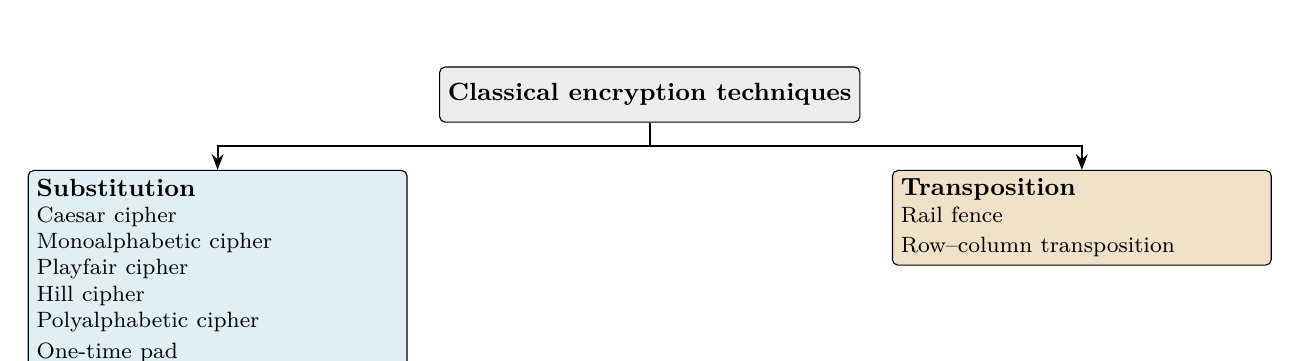
\begin{tikzpicture}[node distance=5mm]
  \node[box,fill=gray!15] (root) {\textbf{Classical encryption techniques}};
  \node[box,fill=cyan!10,below left=6mm and 4mm of root,text width=46mm,align=left] (sub) {\textbf{Substitution}\\
  \footnotesize Caesar cipher\\ \footnotesize Monoalphabetic cipher\\ \footnotesize Playfair cipher\\ \footnotesize Hill cipher\\ \footnotesize Polyalphabetic cipher\\ \footnotesize One-time pad};
  \node[box,fill=yellow!20,below right=6mm and 4mm of root,text width=46mm,align=left] (tra) {\textbf{Transposition}\\
  \footnotesize Rail fence\\ \footnotesize Row--column transposition};
  \draw[arr] (root.south) -- ++(0,-3mm) -| (sub.north);
  \draw[arr] (root.south) -- ++(0,-3mm) -| (tra.north);
\end{tikzpicture}
\end{center}

\section{Caesar Cipher}\label{sec:caesar}

The Caesar cipher is the earliest known and simplest substitution cipher, used by Julius Caesar for military messages. \imp{Each letter of the alphabet is replaced by the letter standing three places further down the alphabet,} and the alphabet is treated as a circle, so that after \ttx{z} it wraps round to \ttx{a}:
\begin{center}\small\ttfamily\setlength{\tabcolsep}{3.2pt}
\begin{tabular}{@{}l*{26}{c}@{}}
\rmfamily plain: & a&b&c&d&e&f&g&h&i&j&k&l&m&n&o&p&q&r&s&t&u&v&w&x&y&z\\
\rmfamily cipher: & D&E&F&G&H&I&J&K&L&M&N&O&P&Q&R&S&T&U&V&W&X&Y&Z&A&B&C\\
\end{tabular}
\end{center}
Since every letter is moved by the same amount and a letter is always replaced by the same letter, it is a monoalphabetic substitution. Stallings' classic example: \ttx{meet me after the toga party} $\to$ \ttx{PHHW PH DIWHU WKH WRJD SDUWB}.

\subsection{Letters as numbers (start at 0)}
To write the rule as a formula, each letter is replaced by its position in the alphabet, starting from 0:
\begin{center}\small\setlength{\tabcolsep}{4pt}
\begin{tabular}{*{13}{c}}
\toprule
A&B&C&D&E&F&G&H&I&J&K&L&M\\
0&1&2&3&4&5&6&7&8&9&10&11&12\\
\midrule
N&O&P&Q&R&S&T&U&V&W&X&Y&Z\\
13&14&15&16&17&18&19&20&21&22&23&24&25\\
\bottomrule
\end{tabular}
\end{center}
Numbering from 0 matches the remainders mod 26, which are exactly $0,1,\dots,25$. The wrap-around from \ttx{z} to \ttx{a} is then simply reduction modulo 26, i.e.\ arithmetic in $\mathbb{Z}_{26}$ (\S\ref{sec:modular}). If the letters were numbered 1 to 26, \ttx{z} would be 26, which reduces to 0, a number that stands for no letter.

\subsection{Algorithm}
With $p$ the number of a plaintext letter, $C$ the number of the ciphertext letter and $k$ the key (the shift), encryption adds the key and decryption subtracts it, both modulo 26.
\begin{mustknow}[: Caesar / shift cipher]
\vspace{-6pt}
\begin{align*}
C &= E(p,k) = (p + k) \bmod 26\\
p &= D(C,k) = (C - k) \bmod 26
\end{align*}
Caesar cipher: $k = 3$. Shift cipher: any $k \in \{1, \dots, 25\}$.
\end{mustknow}

\begin{minipage}[c]{0.55\textwidth}
\textbf{Why decryption works.} Decrypting the encryption gives $\big((p + k) \bmod 26 - k\big) \bmod 26 = p \bmod 26$, because reducing modulo 26 before or after the subtraction gives the same remainder. Since $0 \le p \le 25$, this is exactly $p$.

\textbf{Computing the remainder.} \textbf{mod gives the remainder, not the quotient}: $27 \bmod 26 = 1$, because $27 = 1 \times 26 + 1$. During decryption $C - k$ can be negative; the remainder must lie in $0, \dots, 25$, so add 26: $-2 \bmod 26 = 24$, because $-2 = (-1) \times 26 + 24$.

\textbf{Convention.} Plaintext is written in lowercase and ciphertext in UPPERCASE, which keeps the two apart in a worked answer. For letters away from the end of the alphabet one can simply count $k$ letters forward; the formula matters at the wrap-around.
\end{minipage}\hfill
\begin{minipage}[c]{0.42\textwidth}
\centering
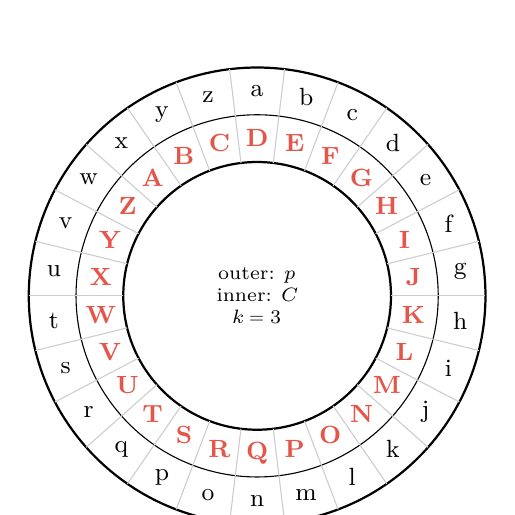
\begin{tikzpicture}
  \draw[thick] (0,0) circle (2.9);
  \draw (0,0) circle (2.3);
  \draw[thick] (0,0) circle (1.7);
  \foreach \pl/\cl [count=\n from 0] in {a/D,b/E,c/F,d/G,e/H,f/I,g/J,h/K,i/L,j/M,k/N,l/O,m/P,n/Q,o/R,p/S,q/T,r/U,s/V,t/W,u/X,v/Y,w/Z,x/A,y/B,z/C}{
    \pgfmathsetmacro{\ang}{90-\n*360/26}
    \pgfmathsetmacro{\sep}{\ang+180/26}
    \node[font=\small] at (\ang:2.6) {\pl};
    \node[font=\small\bfseries,text=warn] at (\ang:2.0) {\cl};
    \draw[gray!50] (\sep:1.7) -- (\sep:2.9);
  }
  \node[font=\scriptsize,align=center] at (0,0) {outer: $p$\\inner: $C$\\$k=3$};
\end{tikzpicture}
\end{minipage}

\subsection{Worked example: encrypt ``neso academy'' ($k=3$)}
\begin{worked}[: Caesar encryption (lecture example)]
\textbf{Q.} Encrypt ``neso academy'' using the Caesar cipher.

\textbf{A.} Convert each letter to its number, add 3, reduce mod 26, convert back:
\begin{center}\small\setlength{\tabcolsep}{5pt}
\begin{tabular}{@{}l*{4}{c}|*{7}{c}@{}}
\toprule
Plaintext & n&e&s&o & a&c&a&d&e&m&y\\
$p$ & 13&4&18&14 & 0&2&0&3&4&12&24\\
$p+3$ & 16&7&21&17 & 3&5&3&6&7&15&\hl{27}\\
$\bmod 26$ & 16&7&21&17 & 3&5&3&6&7&15&\hl{1}\\
Ciphertext & \textbf{Q}&\textbf{H}&\textbf{V}&\textbf{R} & \textbf{D}&\textbf{F}&\textbf{D}&\textbf{G}&\textbf{H}&\textbf{P}&\textbf{B}\\
\bottomrule
\end{tabular}
\end{center}
Answer: \textbf{\ttx{QHVR DFDGHPB}}.
The only wrap-around is \ttx{y}: $24+3 = 27$, and $27 = 26\times 1 + \mathbf{1}$, so $C = 1 = $ \ttx{B}.
(Counting on: y $\to$ z $\to$ a $\to$ \textbf{b}.) For the other letters you can just count three letters forward.
\textbf{Check:} $B = 1$, $1 - 3 = -2 \equiv 24 = $ \ttx{y} \checkmark.
\end{worked}

\subsection{Homework 1: decrypt ``QHWZRUN VHFXULWB'' ($k=3$)}
\begin{worked}[: Caesar decryption (lecture homework)]
\textbf{Q.} Decrypt ``QHWZRUN VHFXULWB'' using the Caesar cipher.

\textbf{A.} Apply $p = (C - 3) \bmod 26$ to every letter:
\begin{center}\small\setlength{\tabcolsep}{3.6pt}
\begin{tabular}{@{}l*{7}{c}|*{8}{c}@{}}
\toprule
Ciphertext & Q&H&W&Z&R&U&N & V&H&F&X&U&L&W&B\\
$C$ & 16&7&22&25&17&20&13 & 21&7&5&23&20&11&22&1\\
$C-3$ & 13&4&19&22&14&17&10 & 18&4&2&20&17&8&19&\hl{$-2$}\\
$\bmod 26$ & 13&4&19&22&14&17&10 & 18&4&2&20&17&8&19&\hl{24}\\
Plaintext & n&e&t&w&o&r&k & s&e&c&u&r&i&t&y\\
\bottomrule
\end{tabular}
\end{center}
Answer: \textbf{network security}. Note the last letter: $1-3=-2$, add 26 $\Rightarrow 24 =$ \ttx{y}.
\end{worked}

\section{Shift Cipher (the general form)}\label{sec:shift}

The Caesar cipher has no real key: the shift is always 3, so anyone who knows the method can read every message. The obvious repair is to let the shift vary and keep it secret. The \textbf{shift cipher} uses the same two formulas with a secret key $k$; Forouzan calls it the \textbf{additive cipher}, because encryption is addition in $\mathbb{Z}_{26}$. \textbf{Caesar cipher = shift cipher with $k=3$.}

\textbf{How many keys?} A key $k$ and the key $k + 26$ give the same cipher, since $(p + k + 26) \bmod 26 = (p + k) \bmod 26$; so every key can be reduced modulo 26 (a shift of 29 is a Caesar shift of 3), and there are only 26 different keys, $0$ to $25$. One of them is useless:
\begin{itemize}
  \item $k=0$ is useless: $C = (p+0) \bmod 26 = p$, so the ciphertext equals the plaintext. (Homework: ``Neso'', $k=0$ $\Rightarrow$ \ttx{NESO}.)
  \item $k=26$ is the same as $k=0$. So there are only \textbf{25 usable keys}.
\end{itemize}

\textbf{Decryption is encryption with $26 - k$.} Subtracting $k$ modulo 26 is the same as adding its additive inverse $26 - k$: $(C - k) \bmod 26 = (C + 26 - k) \bmod 26$. Decrypting the Caesar cipher is therefore the same as encrypting with key 23, and an attacker who tries all forward shifts tries all decryption keys too. This is why the forward and backward shifts in the brute-force table below always add up to 26.

\textbf{Encrypting twice does not help.} Shifting by $k_1$ and then by $k_2$ gives $(p + k_1 + k_2) \bmod 26$, which is a single shift by $(k_1 + k_2) \bmod 26$. Double encryption with two shift keys is just another shift cipher, still with 25 keys to search. (In algebraic terms, the shift ciphers are closed under composition.)

\textbf{Example:} ``Neso'', $k=4$: \;
N $13{+}4{=}17\to$\textbf{R},\;
e $4{+}4{=}8\to$\textbf{I},\;
s $18{+}4{=}22\to$\textbf{W},\;
o $14{+}4{=}18\to$\textbf{S} \;$\Rightarrow$\; \textbf{\ttx{RIWS}}.

\textbf{Homework 2:} ``cryptography'', $k=4$:
\begin{center}\small\setlength{\tabcolsep}{4.5pt}
\begin{tabular}{@{}l*{12}{c}@{}}
\toprule
Plaintext & c&r&y&p&t&o&g&r&a&p&h&y\\
$p$ & 2&17&24&15&19&14&6&17&0&15&7&24\\
$p+4 \bmod 26$ & 6&21&\hl{2}&19&23&18&10&21&4&19&11&\hl{2}\\
Ciphertext & G&V&C&T&X&S&K&V&E&T&L&C\\
\bottomrule
\end{tabular}
\end{center}
Answer: \textbf{\ttx{GVCTXSKVETLC}} (both \ttx{y}'s wrap: $24+4=28 \equiv 2$).

\textbf{In code:} the 0--25 numbering is a convention. With ASCII (\ttx{A}=65, \ttx{a}=97), shift to 0 first, then back:
\;$C = \big((p - 65 + k) \bmod 26\big) + 65$ for uppercase (use 97 for lowercase).

\begin{worked}[: Forouzan Example 3.3 (additive cipher)]
\textbf{Q.} Use the additive cipher with key $= 15$ to encrypt the message ``hello''. Decrypt the result to verify.

\textbf{Encryption}, $C = (p + 15) \bmod 26$:
\begin{center}\small\setlength{\tabcolsep}{6pt}
\begin{tabular}{@{}l*{5}{c}@{}}
\toprule
Plaintext & h&e&l&l&o\\
$p$ & 7&4&11&11&14\\
$p + 15$ & 22&19&\hl{26}&\hl{26}&\hl{29}\\
$\bmod 26$ & 22&19&0&0&3\\
Ciphertext & \textbf{W}&\textbf{T}&\textbf{A}&\textbf{A}&\textbf{D}\\
\bottomrule
\end{tabular}
\qquad
\begin{tabular}{@{}l*{5}{c}@{}}
\toprule
Ciphertext & W&T&A&A&D\\
$C$ & 22&19&0&0&3\\
$C - 15$ & 7&4&\hl{$-15$}&\hl{$-15$}&\hl{$-12$}\\
$\bmod 26$ & 7&4&11&11&14\\
Plaintext & h&e&l&l&o\\
\bottomrule
\end{tabular}
\end{center}
Ciphertext \textbf{\ttx{WTAAD}}; decryption with $p = (C - 15) \bmod 26$ (adding 26 to the negative values) returns \textbf{hello} \checkmark. Note that the double \ttx{l} gives the double \ttx{A}: a monoalphabetic cipher keeps repeated letters visible.
\end{worked}

\subsection{Pros and cons of the Caesar cipher}
\textbf{Advantages.} The cipher is \textbf{simple} and \textbf{easy to implement}: it needs one addition per letter and can be done by hand or written in a few lines of code.

\textbf{Disadvantages.} The lecture lists three, and together they are exactly what makes a brute-force attack succeed.
\begin{enumerate}[leftmargin=1.5em]
  \item \textbf{The encryption and decryption algorithms are known.} By itself this is normal (Kerckhoff's principle, \S\ref{sec:attacks}); it means the attacker knows the cipher is a shift and only has to find $k$.
  \item \textbf{There are only 25 keys to try}, so the cipher is vulnerable to a \textbf{brute-force attack}: trying all of them takes seconds.
  \item \textbf{The language of the plaintext is known and easily recognisable}, so the attacker can tell when he has hit the right key, because exactly one trial produces readable text.
\end{enumerate}
A fourth weakness follows from being monoalphabetic with a single shift: letter frequencies survive, so even without trying keys, one correct guess of a single plaintext--ciphertext letter pair reveals the key (statistical attack below).

\section{Brute-Force Attack on the Caesar/Shift Cipher}\label{sec:bruteforce}

A \textbf{brute-force} (exhaustive key search) attack tries every possible key until readable plaintext appears. For the shift cipher this is trivial. There are 25 keys and the right one is equally likely to be any of them, so on average the attacker needs $(1 + 2 + \cdots + 25)/25 = 13$ trials and at worst 25. By hand that is a few minutes of counting; a computer doing $10^9$ trials per second needs about $10^{-8}$ seconds. Compare $2^{128} \approx 3.4 \times 10^{38}$ keys for AES (\S\ref{sec:schemes}): the attack is the same, only the size of the key space differs.

\begin{mustknow}[: when brute force works (Stallings)]
Three conditions make brute-force cryptanalysis of the Caesar cipher easy: (1) the encryption and decryption algorithms are known; (2) there are only 25 keys to try; (3) the language of the plaintext is known and easily recognisable. A cipher defeats brute force by making (2) false: a key space of $2^{128}$ or more.
\end{mustknow}

\textbf{The lecture example.} Ciphertext: \ttx{SQDYMZK}. Shift every letter forward by 0, 1, 2, \dots, 25 and look for a real word:

\begin{center}\small\ttfamily\setlength{\tabcolsep}{6pt}
\begin{tabular}{@{}ccl@{}}
\toprule
\rmfamily\bfseries Fwd & \rmfamily\bfseries Back & \rmfamily\bfseries Result\\
\midrule
0 & 26 & SQDYMZK\\
1 & 25 & TREZNAL\\
2 & 24 & USFAOBM\\
3 & 23 & VTGBPCN\\
4 & 22 & WUHCQDO\\
5 & 21 & XVIDREP\\
6 & 20 & YWJESFQ\\
7 & 19 & ZXKFTGR\\
8 & 18 & AYLGUHS\\
9 & 17 & BZMHVIT\\
10 & 16 & CANIWJU\\
11 & 15 & DBOJXKV$^\ast$\\
12 & 14 & ECPKYLW\\
\bottomrule
\end{tabular}
\qquad
\begin{tabular}{@{}ccl@{}}
\toprule
\rmfamily\bfseries Fwd & \rmfamily\bfseries Back & \rmfamily\bfseries Result\\
\midrule
13 & 13 & FDQLZMX\\
\rowcolor{warn!18} \textbf{14} & \textbf{12} & \textbf{GERMANY}\\
15 & 11 & HFSNBOZ\\
16 & 10 & IGTOCPA\\
17 & 9 & JHUPDQB\\
18 & 8 & KIVQERC\\
19 & 7 & LJWRFSD\\
20 & 6 & MKXSGTE\\
21 & 5 & NLYTHUF\\
22 & 4 & OMZUIVG$^\ast$\\
23 & 3 & PNAVJWH\\
24 & 2 & QOBWKXI\\
25 & 1 & RPCXLYJ\\
\bottomrule
\end{tabular}
\end{center}
{\footnotesize $^\ast$ Recomputed; the notes had these rows slightly wrong (see corrections box).}

Forward $+$ back $= 26$ in every row, because shifting forward 14 is the same as shifting back 12: $\;C + 14 \equiv C - 12 \pmod{26}$ (\S\ref{sec:shift}). Only one row is English, \textbf{GERMANY}, so the attacker now has the plaintext \emph{and} the key.

\textbf{Which number is the key?} The sender encrypted with $k = \mathbf{12}$ (G $6+12=18=$ S, \dots, Y $24+12=36\equiv10=$ K). The 14 is the forward shift that \emph{undoes} it. The lecture calls 14 ``the key''; be clear which one you mean in an exam: write ``encryption key $k = 12$; decryption is a forward shift of 14 (a backward shift of 12)''.

\textbf{Decryption versus cryptanalysis.} \imp{Decryption is done by the receiver, who has the key and reverses the encryption; cryptanalysis is done by an attacker who does not have the key and recovers the plaintext and/or the key}, here by brute force. The table above is cryptanalysis, not decryption.

\textbf{A caution.} Brute force assumes that exactly one trial gives meaningful text. For a long ciphertext this is practically certain, but a very short ciphertext (three or four letters) may decrypt to two different words under two keys, and then the attacker cannot decide without more ciphertext or context.

\begin{worked}[: Forouzan Example 3.4 (brute force)]
\textbf{Q.} Eve has intercepted the ciphertext \ttx{UVACLYFZLJBYL}. Show how she can use a brute-force attack to break the cipher.

\textbf{A.} Eve knows the cipher is additive and that the key domain is $\{1, \dots, 25\}$. She decrypts with $p = (C - k) \bmod 26$ for $k = 1, 2, 3, \dots$ and stops at the first meaningful text:
\begin{center}\small\setlength{\tabcolsep}{8pt}
\begin{tabular}{@{}cl|cl@{}}
\toprule
Key & Plaintext & Key & Plaintext\\
\midrule
1 & \ttx{tuzbkxeykiaxk} & 5 & \ttx{pqvxgtaugewtg}\\
2 & \ttx{styajwdxjhzwj} & 6 & \ttx{opuwfsztfdvsf}\\
3 & \ttx{rsxzivcwigyvi} & \cellcolor{warn!18}\textbf{7} & \cellcolor{warn!18}\textbf{\ttx{notverysecure}}\\
4 & \ttx{qrwyhubvhfxuh} & & \\
\bottomrule
\end{tabular}
\end{center}
The plaintext is \textbf{``not very secure''} and the key is $\mathbf{k = 7}$. \textbf{Check:} \ttx{n} $= 13$, $13 + 7 = 20 = $ \ttx{U}, the first ciphertext letter \checkmark. (The remaining keys 8--25 were also tried by script; none gives English.)
\end{worked}

\textbf{Statistical attack.} The shift cipher also falls without trying keys. Since every letter is shifted by the same $k$, a single correct pair is enough: if ciphertext letter $c$ stands for plaintext letter $p$, then $k = (c - p) \bmod 26$. The attacker counts the ciphertext letters and assumes the most frequent one stands for \ttx{e}, the most common letter in English (about 12.5\% of letters on the slide's chart; then \ttx{t}, \ttx{a}, \ttx{o}). If the result is not readable, the next most frequent letter is tried as \ttx{e}, or the top letter as \ttx{t}. The attack needs a reasonably long ciphertext, because the frequencies of a short text can differ from the averages.

\begin{worked}[: Forouzan Example 3.5 (statistical attack)]
\textbf{Q.} Eve has intercepted the following ciphertext. Using a statistical attack, find the plaintext.\\
\ttx{XLILSYWIMWRSAJSVWEPIJSVJSYVQMPPMSRHSPPEVWMXMWASVX}\\
\ttx{LQSVILYVVCFIJSVIXLIWIPPIVVIGIMZIWQSVISJJIVW}

\textbf{A.} Count the 92 ciphertext letters. The most frequent are \ttx{I} (14 times), \ttx{V} (13) and \ttx{S} (12). Assume \ttx{I} $\to$ \ttx{e}: $k = (8 - 4) \bmod 26 = \mathbf{4}$. Decrypt with $p = (C - 4) \bmod 26$:
\begin{center}\small
\emph{the house is now for sale for four million dollars it is worth more hurry before the seller receives more offers}
\end{center}
The text is English, so the key is $\mathbf{4}$. \textbf{Check:} \ttx{t} $= 19$, $19 + 4 = 23 = $ \ttx{X} \checkmark. (Taking \ttx{V} as \ttx{e} would give $k = 17$ and gibberish; \ttx{V} actually stands for \ttx{r}, which is unusually common in this text.)
\end{worked}

\begin{trap}[: the usual slips with shift ciphers]
The key space is 25, not 26, since $k = 0$ changes nothing. Show the wrap-around step ($27 \bmod 26 = 1$) and turn a negative value into a remainder by adding 26. In a brute-force answer, draw the table, box the readable row and state the \emph{encryption} key (12 in the \ttx{SQDYMZK} example, not 14). Know the three cons of the Caesar cipher, and do not call ``the algorithm is public'' a violation of Kerckhoff's principle: it is what the principle assumes.
\end{trap}

\begin{fixbox}
\begin{itemize}
  \item ``neso academy'' encrypts to \ttx{QHVR DFDGHPB}. The notes' final answer \ttx{QHVRDFDGHB} drops the \ttx{P}.
  \item Brute-force table: row 11 is \ttx{DBOJXKV} and row 22 is \ttx{OMZUIVG}. Row 12 (\ttx{ECPKYLW}) was already correct.
  \item The notes call con \#1 a ``Kerckhoffs violation''. It isn't: public algorithms are normal (see the intro sheet). The problem is a public algorithm \emph{plus} only 25 keys.
  \item Slide typo: ``used \emph{be} Julius Caesar'' $\to$ ``used \emph{by}''.
  \item Shift-cipher slide: ``Key = 2, 3, 4, 5, \dots'' leaves out $k = 1$, which is a valid key; the usable keys are $1, \dots, 25$.
\end{itemize}
\end{fixbox}

% Sources: Neso videos (monoalphabetic; Playfair parts 1-2; Playfair solved question; crypto/notes3.md), college Lecture 5
% (Forouzan 3.2: monoalphabetic key table, statistical attack, Playfair secret key and "hello", cryptanalysis of Playfair),
% Stallings 2.2 (frequency analysis, homophones, Playfair strength). Every number recomputed by script (scratchpad/r2/verify.py).
\providecommand{\NESOACADEMY}{{N,E,S,O,A},{C,D,M,Y,B},{F,G,H,{I/J},K},{L,P,Q,R,T},{U,V,W,X,Z}}
\providecommand{\JUPITER}{{{I/J},U,P,T,E},{R,A,B,C,D},{F,G,H,K,L},{M,N,O,Q,S},{V,W,X,Y,Z}}
\providecommand{\NESOAPP}{{N,E,S,O,A},{P,B,C,D,F},{G,H,{I/J},K,L},{M,Q,R,T,U},{V,W,X,Y,Z}}
\providecommand{\PFFOROUZAN}{{L,G,D,B,A},{Q,M,H,E,C},{U,R,N,{I/J},F},{X,V,S,O,K},{Z,Y,W,T,P}}

\section{Monoalphabetic Cipher}\label{sec:monoalpha}

The Caesar (shift) cipher has two weaknesses that make it useless. Its key space has only 25 useful keys, so an attacker simply tries them all. Worse, every letter is shifted by the \emph{same} amount, so the shift found for a single letter decrypts the whole message. The monoalphabetic cipher removes both weaknesses at once: instead of shifting the alphabet, it replaces each letter by an \emph{arbitrary} other letter, chosen independently for each of the 26 letters. The only constraint is that the replacement must be one-to-one, so that the receiver can undo it.

\subsection{Permutations}
A \imp{permutation of a finite set $S$ is an ordered sequence of all the elements of $S$, with each element appearing exactly once.} The set $S = \{a, b, c\}$ has six permutations: \ttx{abc, acb, bac, bca, cab, cba}. In general a set of $n$ elements has $n! = n(n-1)\cdots 2 \cdot 1$ permutations, because the first position can be filled in $n$ ways, the second in $n - 1$ ways (one element is used up), and so on down to one way for the last position. For example $2! = 2$ and $4! = 24$.

Permutations matter here because the key of a monoalphabetic cipher \emph{is} a permutation of the alphabet: writing the ciphertext letters for $a, b, \dots, z$ in order gives a sequence in which each of the 26 letters appears exactly once. The number of possible keys is therefore the number of permutations of 26 letters, $26!$.

\subsection{The cipher}
In a \textbf{monoalphabetic substitution cipher} Alice and Bob agree on a table that pairs every plaintext letter with one ciphertext letter. The bottom row of the table, the \textbf{cipher line}, can be any permutation of the 26 letters. To encrypt, each plaintext letter is looked up in the top row and replaced by the letter below it; to decrypt, each ciphertext letter is found in the bottom row and replaced by the letter above it. The relationship between plaintext and ciphertext symbols is \textbf{one-to-one}: a plaintext letter always becomes the same ciphertext letter, and no two plaintext letters share a ciphertext letter. If two letters shared one, the receiver could not tell which was meant, so the table would not be decryptable.

The key space has $26! \approx 4.03 \times 10^{26} \approx 2^{88}$ keys, compared with 25 for the shift cipher. A computer testing $10^{12}$ keys per second would need about 13 million years to try them all, so the slide's conclusion is that the large key space ``would seem to eliminate brute-force techniques''. The shift ciphers are just 26 of these $26!$ permutations, those in which the cipher line is the alphabet rotated. Although a permutation is involved, the monoalphabetic cipher is still a \textbf{substitution} cipher: the permutation is applied to the \emph{alphabet} to build the key, while the letters of the message keep their positions. Rearranging the message itself would be a transposition.

\textbf{Example (lecture).} Under one key, ``Neso'' becomes \ttx{DULA}. The distance each letter moves is different, so learning one pair of the table says nothing about the others; with Caesar the distance is always 3.
\begin{center}\small\setlength{\tabcolsep}{6pt}
\begin{tabular}{@{}lcccc@{}}
\toprule
Plaintext & N (13) & E (4) & S (18) & O (14)\\
Ciphertext & \textbf{D} (3) & \textbf{U} (20) & \textbf{L} (11) & \textbf{A} (0)\\
Shift $(C-p) \bmod 26$ & 16 & 16 & 19 & 12\\
\bottomrule
\end{tabular}
\end{center}

\begin{worked}[: the slide's key table (Forouzan)]
\textbf{Q.} Using the key below, encrypt ``this message is easy to encrypt but hard to find the key'', and show how Bob decrypts.
\begin{center}\small\setlength{\tabcolsep}{2.4pt}
\begin{tabular}{@{}l*{26}{c}@{}}
\toprule
Plain & a&b&c&d&e&f&g&h&i&j&k&l&m&n&o&p&q&r&s&t&u&v&w&x&y&z\\
Cipher & N&O&A&T&R&B&E&C&F&U&X&D&Q&G&Y&L&K&H&V&I&J&M&P&Z&S&W\\
\bottomrule
\end{tabular}
\end{center}
\textbf{A.} Remove the spaces and replace each letter by the one below it: t$\to$I, h$\to$C, i$\to$F, s$\to$V, so ``this'' $\to$ \ttx{ICFV}; ``message'' $\to$ \ttx{QRVVNER}; and so on. The ciphertext is
\begin{center}\small\ttfamily ICFVQRVVNERFVRNVSIYRGAHSLIOJICNHTIYBFGTICRXRS\end{center}
Bob finds each ciphertext letter in the bottom row and reads the letter above it (I$\to$t, C$\to$h, F$\to$i, V$\to$s, \dots), which recovers the plaintext. Note that the three \ttx{s} of ``message is'' all became \ttx{V} and every \ttx{e} became \ttx{R}: the frequency pattern of the plaintext survives, which is the subject of the next subsection.
\end{worked}

\subsection{Breaking it: frequency analysis}
The huge key space does not protect the cipher, because the attacker never searches through keys. A monoalphabetic cipher only \emph{renames} letters. If the key maps $x$ to $\pi(x)$, then every occurrence of $x$ in the plaintext becomes an occurrence of $\pi(x)$ in the ciphertext and nothing else becomes $\pi(x)$, so $\pi(x)$ occurs in the ciphertext exactly as often as $x$ occurs in the plaintext. The histogram of ciphertext letters is the histogram of plaintext letters with the bars relabelled. \imp{A monoalphabetic cipher does not change the frequency of characters}, so each letter of the key can be found separately by matching frequencies, and the attack needs a few dozen decisions instead of $26!$ guesses. This is a \textbf{statistical} (frequency) attack, and it needs only the ciphertext, which makes it a ciphertext-only attack, the most likely kind in practice.

The attack works because English letters are far from equally common. The relative frequencies (lecture chart, from a large corpus) are:
\begin{center}
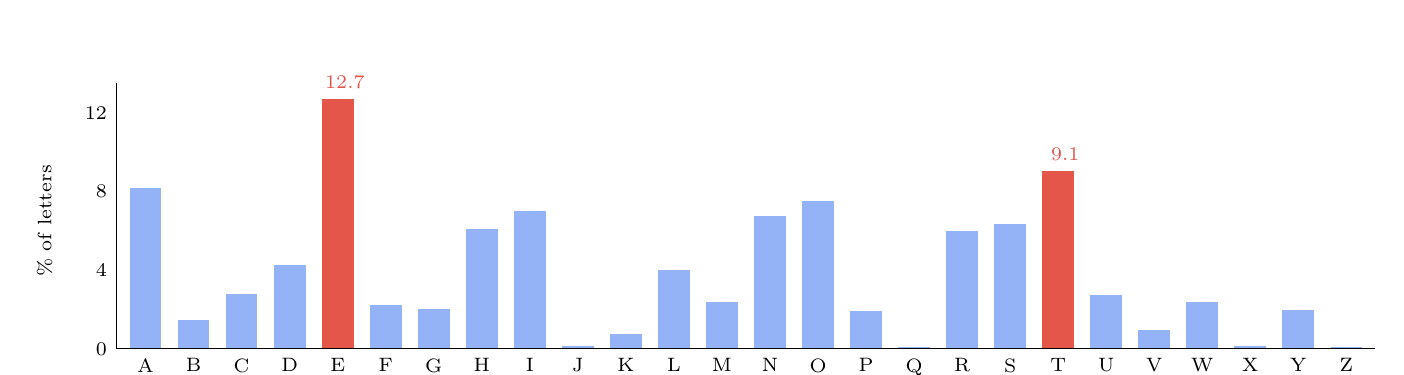
\begin{tikzpicture}[x=6.1mm,y=2.5mm]
  \foreach \L/\v [count=\i] in {A/8.167,B/1.492,C/2.782,D/4.253,E/12.702,F/2.228,G/2.015,H/6.094,I/6.996,J/0.153,K/0.772,L/4.025,M/2.406,N/6.749,O/7.507,P/1.929,Q/0.095,R/5.987,S/6.327,T/9.056,U/2.758,V/0.978,W/2.360,X/0.150,Y/1.974,Z/0.074}{
    \fill[acc!55] (\i-0.33,0) rectangle (\i+0.33,\v);
    \node[font=\scriptsize,below] at (\i,0) {\L};
  }
  \fill[warn] (5-0.33,0) rectangle (5.33,12.702) node[above,font=\scriptsize,xshift=-1.1mm] {12.7};
  \fill[warn] (20-0.33,0) rectangle (20.33,9.056) node[above,font=\scriptsize,xshift=-1.1mm] {9.1};
  \draw (0.4,0) -- (26.6,0);
  \draw (0.4,0) -- (0.4,13.5);
  \foreach \y in {0,4,8,12} \node[font=\scriptsize,left] at (0.4,\y) {\y};
  \node[font=\scriptsize,rotate=90] at (-1.1,6.5) {\% of letters};
\end{tikzpicture}
\end{center}
Ranked from most to least common, the letters are
\begin{center}
\ttx{e t a o i n s h r d l c u m w f g y p b v k j x q z}.
\end{center}
The letter \ttx{e} alone is 12.7\% of English text and \ttx{t} is 9.1\%; the nine letters \ttx{e t a o i n s h r} together make up about 70\% of it, while \ttx{j, x, q, z} are each below 0.2\%. Pairs and triples are just as uneven. The most common \textbf{digrams} (two-letter groups) are \ttx{th, he, in, er, an, re, ed, on, es, st, en, at, to, nt, ha, nd, ou, ea, ng, as, or, ti, is, et, it, ar, te, se, hi, of}, and the most common \textbf{trigrams} are \ttx{the, ing, and, her, ere, ent, tha, nth, was, eth, for, dth} (lecture table, from Forouzan).

The attack therefore proceeds as follows. Eve counts the ciphertext letters and guesses that the most frequent one stands for \ttx{e} and the next for \ttx{t}. She then tests the guesses against digrams and trigrams: if \ttx{t} has been placed, a frequent pattern ``\ttx{t?e}'' is almost certainly \ttx{the}, which reveals \ttx{h}. Each new letter makes more words partly readable, and the remaining letters are filled in by recognising words. The statistics only become reliable with enough text: with about 100 letters the top two or three ranks usually match English, while the lower ranks are shuffled and have to be fixed by word guessing. For a very short message the counts may mislead completely.

\begin{worked}[: the lecture's frequency attack (Stallings' ciphertext, 120 letters)]
\textbf{Q.} The following ciphertext was produced by a monoalphabetic cipher. Use a statistical attack to find the plaintext.
\begin{center}\small\ttfamily
UZQSOVUOHXMOPVGPOZPEVSGZWSZOPFPESXUDBMETSXAIZ\\
VUEPHZHMDZSHZOWSFPAPPDTSVPQUZWYMXUZUHSX\\
EPYEPOPDZSZUFPOMBZWPFUPZHMDJUDTMOHMQ
\end{center}
\textbf{A. Step 1: count.} The 120 letters occur as follows (C, K, L, N, R do not occur):
\begin{center}\small\setlength{\tabcolsep}{3pt}
\begin{tabular}{@{}l*{21}{c}@{}}
\toprule
Letter & \textbf{P}&\textbf{Z}&S&U&O&M&H&D&E&V&X&F&W&Q&T&A&B&G&Y&I&J\\
Count & 16&14&10&10&9&8&7&6&6&5&5&4&4&3&3&2&2&2&2&1&1\\
\bottomrule
\end{tabular}
\end{center}
\textbf{Step 2: the two peaks.} \ttx{P} is $16/120 = 13.33\%$ and \ttx{Z} is $14/120 = 11.67\%$, close to the 12.7\% of \ttx{e} and 9.1\% of \ttx{t}. Guess \ttx{P} $=$ e and \ttx{Z} $=$ t.

\textbf{Step 3: digrams and trigrams.} The digram \ttx{ZW} occurs 3 times, and \ttx{ZWP} once. With the guesses this is ``t?e'', so \ttx{ZWP} $=$ ``the'' and \ttx{W} $=$ h. Then \ttx{ZWS} $=$ ``th?'', which fits ``that'', so \ttx{S} $=$ a.

\textbf{Step 4: fill in.} With \ttx{e, t, h, a} placed, $16 + 14 + 4 + 10 = 44$ of the 120 letters (37\%) are known and words become guessable. For example, \ttx{ZWSZ OPFPESX} now reads ``that ?e?e?a?'', which suggests ``that several'' and gives \ttx{O} $=$ s, \ttx{F} $=$ v, \ttx{E} $=$ r, \ttx{X} $=$ l. Each guess is checked against the rest of the text, and the remaining letters follow in the same way. The result is
\begin{center}\small
\emph{it was disclosed yesterday that several informal but direct contacts have been made with political representatives of the viet cong in moscow}
\end{center}
and the recovered key (cipher $\to$ plain) is
\begin{center}\small\setlength{\tabcolsep}{2.6pt}
\begin{tabular}{@{}l*{21}{c}@{}}
\toprule
Cipher & A&B&D&E&F&G&H&I&J&M&O&\textbf{P}&Q&S&T&U&V&\textbf{W}&X&Y&\textbf{Z}\\
Plain  & b&f&n&r&v&y&c&u&g&o&s&\textbf{e}&w&a&m&i&d&\textbf{h}&l&p&\textbf{t}\\
\bottomrule
\end{tabular}
\end{center}
\textbf{Check:} applying this table to all 120 letters gives the sentence above. Note that \ttx{S} (a) and \ttx{U} (i) tie at 10, ahead of \ttx{O} (s) at 9: below the top two ranks, a short text does not follow the English ranking exactly, which is why steps 3--4 are needed.
\end{worked}

\subsection{Pros, cons, countermeasure}
\textbf{Advantages.} The monoalphabetic cipher is as simple to use as the Caesar cipher, but its key space of $26!$ makes brute force impossible, and knowing one letter's substitute reveals nothing about the others. It is therefore much more secure than the Caesar cipher against an attacker who only tries keys.

\textbf{Disadvantages.} Since the ciphertext reflects the frequency data of the original alphabet, the cipher is easy to break with frequency analysis; the guessing attack above needs only a short ciphertext and some knowledge of English letter frequencies. The key is also long (a full table of 26 letters) and awkward to share and memorise, which is why practical versions derive it from a key phrase (see the homework below).

\textbf{Countermeasure: homophones.} A \textbf{homophonic substitution} gives each plaintext letter several possible ciphertext symbols, called \textbf{homophones}, and the encryptor picks one of them at random for each occurrence. The number of homophones is made proportional to the letter's frequency: \ttx{e} (about 13\%) gets about 13 symbols, while \ttx{z} gets one. Since each of the 13 symbols for \ttx{e} is then used for roughly $12.7/13 \approx 1\%$ of the text, every symbol appears with about the same frequency and the peaks in the histogram disappear. The ciphertext alphabet must be larger than 26, for example the numbers 00 to 99. Decryption is still unique, because each symbol belongs to only one plaintext letter.

Homophones flatten the \emph{single-letter} frequencies, but they do not make the cipher secure. Each plaintext letter still affects only one ciphertext symbol, so multi-letter patterns survive: \ttx{t} is still very often followed by \ttx{h}, so the symbols of \ttx{t} are often followed by symbols of \ttx{h}, and the attacker can group the symbols that behave alike and then proceed as before. Two better remedies were developed from this observation: encrypting \emph{several letters together} (Playfair, Hill), and using \emph{several cipher alphabets} chosen by a key (the polyalphabetic ciphers of \S\ref{sec:poly}).

\subsection{Homework: encrypt with a key phrase}
Since a random 26-letter table is hard to remember, the key is often derived from a key phrase: write the phrase without spaces, delete every letter that has already appeared, and use the result as the cipher line. If the phrase does not contain all 26 letters, the unused letters are appended in alphabetical order (exactly as in the Playfair square below).

\begin{worked}[: lecture homework]
\textbf{Q.} Encrypt ``Attack postponed to tomorrow and do not use our secret paper until further info'' with a monoalphabetic cipher whose key is ``The quick brown fox jumps over the lazy dog'' (ignore the second and later occurrences of a letter in the key).

\textbf{A.} Removing spaces and repeated letters from the key phrase leaves \ttx{THEQUICKBROWNFXJMPSVLAZYDG}. The phrase is a pangram, so this already contains all 26 letters and is the whole cipher line:
\begin{center}\small\setlength{\tabcolsep}{2.4pt}
\begin{tabular}{@{}l*{26}{c}@{}}
\toprule
Plain & a&b&c&d&e&f&g&h&i&j&k&l&m&n&o&p&q&r&s&t&u&v&w&x&y&z\\
Cipher & T&H&E&Q&U&I&C&K&B&R&O&W&N&F&X&J&M&P&S&V&L&A&Z&Y&D&G\\
\bottomrule
\end{tabular}
\end{center}
Substituting letter by letter (spaces kept only for readability):
\begin{center}\small\ttfamily
TVVTEO JXSVJXFUQ VX VXNXPPXZ TFQ QX FXV LSU XLP SUEPUV JTJUP LFVBW ILPVKUP BFIX
\end{center}
\textbf{Check} on the first word: a$\to$T, t$\to$V, t$\to$V, a$\to$T, c$\to$E, k$\to$O gives \ttx{TVVTEO}. The doubled \ttx{tt} became the doubled \ttx{VV}, another pattern a monoalphabetic cipher cannot hide.
\end{worked}

%%PLAYFAIR%%

% Sources: Neso videos (Hill encryption, Hill decryption, Vigenere & autokey, Vernam; crypto/notes4.md), college Lecture 5
% (Forouzan 3.2: Hill 4x4 "code is ready", cryptanalysis of Hill, Vigenere "She is listening", Kasiski, autokey
% "Attack is today"), Stallings 2.2 (Hill known-plaintext "hillcipher", Vigenere/autokey "deceptive", Vernam).
% Every number recomputed by script (scratchpad/r2/verify.py, verify2.py).
\section{Hill Cipher}\label{sec:hill}
\likely{Hill encryption with a $2\times2$ or $3\times3$ key, then $K^{-1}$ and decryption (5--8 marks); or the known-plaintext attack $K = P^{-1}C$ (3--4 marks).}

Playfair hides single-letter frequencies, but it works only on pairs, its rules are fixed geometric moves, and each digram always has the same substitute, so digram statistics still leak. The \textbf{Hill cipher}, published by the mathematician \textbf{Lester Hill in 1929}, generalises the idea to blocks of any size $m$ and replaces the geometric rules by linear algebra modulo 26. Each ciphertext letter of a block is a weighted sum of \emph{all} $m$ plaintext letters of that block, so the same plaintext letter becomes different ciphertext letters depending on its neighbours, and for $m \ge 3$ even digram frequencies are hidden. It is a \textbf{multiletter} (polygraphic) substitution cipher: $m = 2$ encrypts digraphs, $m = 3$ trigraphs, general $m$ polygraphs. Because every character of a block contributes to the encryption of every other character of the block, Forouzan classifies Hill as a \textbf{block cipher}, while the letter-by-letter ciphers before it are stream ciphers.

The mathematics needed is matrix multiplication modulo 26 for encryption, and the determinant and the multiplicative inverse modulo 26 for decryption.

\subsection{Encryption: matrix multiplication mod 26}
The letters are numbered $a = 0, \dots, z = 25$. The plaintext is cut into blocks of $m$ letters (the last block is padded with a filler such as \ttx{x}), and each block is written as a \textbf{row vector} $P = (P_1\;P_2\;\cdots\;P_m)$. The key is an $m \times m$ matrix $K$ with entries in $\mathbb{Z}_{26}$. A block is encrypted by multiplying it by the key and reducing every entry modulo 26; decryption multiplies by the inverse matrix.

\begin{mustknow}[: Hill cipher]
\vspace{-6pt}
\[
\text{Encrypt: } C = PK \bmod 26 \qquad\qquad \text{Decrypt: } P = CK^{-1} \bmod 26, \qquad K^{-1} = (\det K)^{-1} \cdot \operatorname{adj}(K) \bmod 26
\]
Decryption works because $CK^{-1} = (PK)K^{-1} = P(KK^{-1}) = PI = P$. The key is valid only if $\gcd(\det K, 26) = 1$.
\end{mustknow}

For $m = 3$ the multiplication written out is
\[
(C_1\;C_2\;C_3) = (P_1\;P_2\;P_3)\begin{pmatrix}K_{11}&K_{12}&K_{13}\\K_{21}&K_{22}&K_{23}\\K_{31}&K_{32}&K_{33}\end{pmatrix} \bmod 26
\qquad
\begin{aligned}
C_1 &= (P_1K_{11}+P_2K_{21}+P_3K_{31}) \bmod 26\\
C_2 &= (P_1K_{12}+P_2K_{22}+P_3K_{32}) \bmod 26\\
C_3 &= (P_1K_{13}+P_2K_{23}+P_3K_{33}) \bmod 26
\end{aligned}
\]
The sizes are $(1\times3)(3\times3) = (1\times3)$, and each $C_j$ is the plaintext row multiplied entry by entry with column $j$ of $K$ and summed. The equations show directly that every ciphertext letter depends on every plaintext letter of the block.

\textbf{$PK$ vs.\ $KP$.} This lecture and Forouzan use $C = PK$ (plaintext as a row). Some books (and some exam papers) write the plaintext as a \textbf{column} vector: then $C = KP$ and decryption is $P = K^{-1}C$. The two conventions give different ciphertexts for the same key (column-vector encryption with $K$ is row-vector encryption with the transpose $K^T$), so state the convention and use it consistently.

\subsection{Which matrices can be keys}
Not every square matrix has an inverse modulo 26, and a key without one is useless, because Bob could not decrypt. The test comes from the \textbf{adjugate} $\operatorname{adj}(K)$, the transpose of the matrix of cofactors $C_{ij} = (-1)^{i+j} M_{ij}$, where the minor $M_{ij}$ is the determinant of $K$ with row $i$ and column $j$ deleted. Over the integers every square matrix satisfies
\[
K \cdot \operatorname{adj}(K) = \det(K) \cdot I
\]
(for the key in the next example, $K \cdot \operatorname{adj}(K) = -939\, I$, checked). If $\det K$ has a multiplicative inverse modulo 26, multiplying both sides by it gives $K \cdot \big((\det K)^{-1}\operatorname{adj}(K)\big) \equiv I$, which is the formula for $K^{-1}$. Conversely, if $K^{-1}$ exists then $\det(K)\det(K^{-1}) = \det(I) = 1 \pmod{26}$, so $\det K$ must be invertible. Hence \imp{a Hill key is valid if and only if $\gcd(\det K \bmod 26, 26) = 1$}, i.e.\ $\det K \bmod 26$ is odd and not 13. Only 12 of the 26 values qualify: $1, 3, 5, 7, 9, 11, 15, 17, 19, 21, 23, 25$.

When the condition fails, encryption is not one-to-one. With $K = \begin{pmatrix}2&0\\0&1\end{pmatrix}$ ($\det K = 2$), the blocks \ttx{aa} $= (0, 0)$ and \ttx{na} $= (13, 0)$ both encrypt to $(0, 0) = $ \ttx{AA}, because $13 \cdot 2 = 26 \equiv 0$. Bob, receiving \ttx{AA}, cannot know which was sent.

\textbf{Key space.} The slides count $26^{m \times m}$ matrices ($26^9 \approx 5.4 \times 10^{12}$ for $m = 3$, $26^{16} \approx 4.4 \times 10^{22}$ for $m = 4$). Only the invertible ones are keys (157{,}248 of the 456{,}976 matrices for $m = 2$), but the count grows so fast with $m$ that brute force on a large key is hopeless.

\subsection{Encryption example: ``pay more money''}
\begin{worked}[: lecture / Stallings]
\textbf{Q.} Encrypt ``pay more money'' with the Hill cipher, $C = PK \bmod 26$, \;$K = \begin{pmatrix}17&17&5\\21&18&21\\2&2&19\end{pmatrix}$.

\textbf{A.} $m = 3$, so the 12 letters form four blocks \ttx{pay | mor | emo | ney} (no padding needed). Block 1, \ttx{pay} $= (15\;0\;24)$:
\[
\begin{aligned}
C_1 &= 15\cdot17 + 0\cdot21 + 24\cdot2 = 255+0+48 = 303 = 11\cdot26 + \mathbf{17} &&\to \ttx{R}\\
C_2 &= 15\cdot17 + 0\cdot18 + 24\cdot2 = 255+0+48 = 303 \equiv \mathbf{17} &&\to \ttx{R}\\
C_3 &= 15\cdot5 + 0\cdot21 + 24\cdot19 = 75+0+456 = 531 = 20\cdot26 + \mathbf{11} &&\to \ttx{L}
\end{aligned}
\]
\begin{center}\small
\begin{tabular}{@{}lcccc@{}}
\toprule
Block & $P$ & $PK$ (before mod) & $\bmod 26$ & Ciphertext\\
\midrule
pay & (15, 0, 24) & (303, 303, 531) & (17, 17, 11) & \textbf{RRL}\\
mor & (12, 14, 17) & (532, 490, 677) & (12, 22, 1) & \textbf{MWB}\\
emo & (4, 12, 14) & (348, 312, 538) & (10, 0, 18) & \textbf{KAS}\\
ney & (13, 4, 24) & (353, 341, 605) & (15, 3, 7) & \textbf{PDH}\\
\bottomrule
\end{tabular}
\end{center}
Answer: \textbf{\ttx{RRLMWBKASPDH}}. \textbf{Check:} decryption below returns \ttx{pay more money}.
\end{worked}

\subsection{Decryption: finding $K^{-1}$}
By the previous subsection, $K^{-1} = (\det K)^{-1} \cdot \operatorname{adj}(K) \bmod 26$, and the computation is done in four steps, each of which should be shown in an exam answer: (1) $\det K \bmod 26$; (2) its multiplicative inverse modulo 26, which exists only if $\gcd(\det K, 26) = 1$; (3) $\operatorname{adj}(K) \bmod 26$; (4) the product of (2) and (3), reduced modulo 26, followed by the check $KK^{-1} \equiv I$.

\textbf{Step 1: determinant} (expand along row 1, signs $+\,-\,+$):
\[
\det K = 17\begin{vmatrix}18&21\\2&19\end{vmatrix} - 17\begin{vmatrix}21&21\\2&19\end{vmatrix} + 5\begin{vmatrix}21&18\\2&2\end{vmatrix}
= 17(300) - 17(357) + 5(6) = 5100 - 6069 + 30 = -939
\]
$-939 = -36\cdot26 - 3$, so $\det K \equiv -3 \equiv -3 + 26 = \mathbf{23} \pmod{26}$. Since 23 is odd and not 13, the key is valid.

\textbf{Step 2: inverse of 23 mod 26.} Find $x$ with $23x \bmod 26 = 1$ by trying $x = 1, 2, 3, \dots$ (or by the extended Euclidean algorithm, \S\ref{sec:exteuclid}):
\begin{center}\small\setlength{\tabcolsep}{3.2pt}
\begin{tabular}{@{}l*{17}{c}@{}}
\toprule
$x$ & 1&2&3&4&5&6&7&8&9&10&11&12&13&14&15&16&\hl{17}\\
$23x \bmod 26$ & 23&20&17&14&11&8&5&2&25&22&19&16&13&10&7&4&\hl{1}\\
\bottomrule
\end{tabular}
\end{center}
$23 \times 17 = 391 = 15\cdot26 + 1$, so $\mathbf{23^{-1} \equiv 17}$.

\textbf{Step 3: adjugate, using the $5\times5$ shortcut.} Computing nine cofactors and transposing is error-prone; the lecture's grid produces the adjugate directly, with the signs and the transpose built in.
\begin{enumerate}[leftmargin=1.5em]
  \item Copy the first two columns to the right, then the first two rows to the bottom ($5\times5$).
  \item Delete the first row and first column. That leaves a $4\times4$ grid.
  \item Slide a $2\times2$ window over the grid. Each window gives $ad - bc$.
  \textbf{Columns 1--2 of the grid give row 1 of $\operatorname{adj}K$} (windows at rows 1--2, 2--3, 3--4); columns 2--3 give row 2; columns 3--4 give row 3. The signs come out automatically.
\end{enumerate}
\begin{center}\small
\begin{tabular}{ccccc}
\color{gray}17&\color{gray}17&\color{gray}5&\color{gray}17&\color{gray}17\\
\color{gray}21&18&21&21&18\\
\color{gray}2&2&19&2&2\\
\color{gray}17&17&5&17&17\\
\color{gray}21&18&21&21&18
\end{tabular}
\quad$\Rightarrow$\quad
\begin{tabular}{|cc|cc|}
\hline
\cellcolor{cyan!20}18&\cellcolor{cyan!20}21&21&18\\
\cellcolor{cyan!20}2&\cellcolor{cyan!20}19&2&2\\
17&5&17&17\\
18&21&21&18\\
\hline
\end{tabular}
\quad
{\footnotesize first window: $18\cdot19 - 21\cdot2 = 300$}
\end{center}
\[
\operatorname{adj}K =
\begin{pmatrix}
18\cdot19-21\cdot2 & 2\cdot5-19\cdot17 & 17\cdot21-5\cdot18\\
21\cdot2-21\cdot19 & 19\cdot17-2\cdot5 & 5\cdot21-17\cdot21\\
21\cdot2-18\cdot2 & 2\cdot17-2\cdot17 & 17\cdot18-17\cdot21
\end{pmatrix}
=
\begin{pmatrix}300&-313&267\\-357&313&-252\\6&0&-51\end{pmatrix}
\]
\[
\equiv
\begin{pmatrix}14&-1&7\\-19&1&-18\\6&0&-25\end{pmatrix}
\equiv
\begin{pmatrix}14&25&7\\7&1&8\\6&0&1\end{pmatrix} \pmod{26}
\]
(Reduce mod 26, then add 26 to each negative: $-1\to25$, $-19\to7$, $-18\to8$, $-25\to1$.) The shortcut agrees with the cofactor definition: for example the entry in row 1, column 2 is the cofactor $C_{21} = -\begin{vmatrix}17&5\\2&19\end{vmatrix} = -(323 - 10) = -313$.

\textbf{Step 4: combine.}
\[
K^{-1} = 17\begin{pmatrix}14&25&7\\7&1&8\\6&0&1\end{pmatrix}
= \begin{pmatrix}238&425&119\\119&17&136\\102&0&17\end{pmatrix}
\equiv \boxed{\begin{pmatrix}4&9&15\\15&17&6\\24&0&17\end{pmatrix}} \pmod{26}
\]
Check: $KK^{-1} = \begin{pmatrix}443&442&442\\858&495&780\\494&52&365\end{pmatrix} \equiv \begin{pmatrix}1&0&0\\0&1&0\\0&0&1\end{pmatrix} = I$ \checkmark\;
($443 = 17\cdot26+1$, $442 = 17\cdot26$, \dots)

\subsection{Decryption example: \ttx{RRLMWBKASPDH}}
\begin{worked}[: lecture]
\textbf{Q.} Decrypt \ttx{RRLMWBKASPDH} with the key of the previous example.

\textbf{A.} Multiply each ciphertext block by $K^{-1}$ found above and reduce mod 26:
\begin{center}\small
\begin{tabular}{@{}lcccc@{}}
\toprule
Block & $C$ & $CK^{-1}$ (before mod) & $\bmod 26$ & Plaintext\\
\midrule
RRL & (17, 17, 11) & (587, 442, 544) & (15, 0, 24) & \textbf{pay}\\
MWB & (12, 22, 1) & (402, 482, 329) & (12, 14, 17) & \textbf{mor}\\
KAS & (10, 0, 18) & (472, 90, 456) & (4, 12, 14) & \textbf{emo}\\
PDH & (15, 3, 7) & (273, 186, 362) & (13, 4, 24) & \textbf{ney}\\
\bottomrule
\end{tabular}
\end{center}
e.g.\ $P_1 = 17\cdot4 + 17\cdot15 + 11\cdot24 = 68 + 255 + 264 = 587 = 22\cdot26 + 15 \to \ttx{p}$.\quad Answer: \textbf{pay more money}.
\end{worked}

\subsection{A $2\times2$ example}
For $m = 2$ the inverse has a closed form. If $K = \begin{pmatrix}a&b\\c&d\end{pmatrix}$, then $\det K = ad - bc$ and $\operatorname{adj}K = \begin{pmatrix}d&-b\\-c&a\end{pmatrix}$ (swap the diagonal, negate the other two entries), so
\[
K^{-1} = (ad - bc)^{-1}\begin{pmatrix}d&-b\\-c&a\end{pmatrix} \bmod 26 .
\]

\begin{worked}[: new, Forouzan exercise style]
\textbf{Q.} Using the Hill cipher with $C = PK \bmod 26$ and $K = \begin{pmatrix}5&8\\17&3\end{pmatrix}$, encrypt ``exam''. Find $K^{-1}$ and decrypt the result.

\textbf{Encrypt.} Blocks \ttx{ex} $= (4, 23)$ and \ttx{am} $= (0, 12)$.
\begin{center}\small
\begin{tabular}{@{}lll@{}}
\toprule
Block & $PK$ & mod 26\\
\midrule
ex & $(4\cdot5 + 23\cdot17,\; 4\cdot8 + 23\cdot3) = (411, 101)$ & $(21, 23) =$ \ttx{VX}\\
am & $(0\cdot5 + 12\cdot17,\; 0\cdot8 + 12\cdot3) = (204, 36)$ & $(22, 10) =$ \ttx{WK}\\
\bottomrule
\end{tabular}
\end{center}
Ciphertext: \textbf{\ttx{VXWK}}. ($411 = 15\cdot26 + 21$, $101 = 3\cdot26 + 23$, $204 = 7\cdot26 + 22$.)

\textbf{Inverse.} $\det K = 5\cdot3 - 8\cdot17 = 15 - 136 = -121 = -5\cdot26 + 9 \equiv 9$; $\gcd(9, 26) = 1$, so the key is valid. $9^{-1} \equiv 3$ since $9 \cdot 3 = 27 = 26 + 1$.
\[
K^{-1} = 3\begin{pmatrix}3&-8\\-17&5\end{pmatrix} = \begin{pmatrix}9&-24\\-51&15\end{pmatrix} \equiv \begin{pmatrix}9&2\\1&15\end{pmatrix} \pmod{26}.
\]
Check: $KK^{-1} = \begin{pmatrix}5\cdot9+8\cdot1 & 5\cdot2+8\cdot15\\17\cdot9+3\cdot1 & 17\cdot2+3\cdot15\end{pmatrix} = \begin{pmatrix}53&130\\156&79\end{pmatrix} \equiv I$ \checkmark\ ($53 = 2\cdot26+1$, $130 = 5\cdot26$, $156 = 6\cdot26$, $79 = 3\cdot26+1$).

\textbf{Decrypt.} \ttx{VX}: $(21\cdot9 + 23\cdot1,\; 21\cdot2 + 23\cdot15) = (212, 387) \equiv (4, 23) =$ \ttx{ex}. \;\ttx{WK}: $(22\cdot9 + 10\cdot1,\; 22\cdot2 + 10\cdot15) = (208, 194) \equiv (0, 12) =$ \ttx{am}. Plaintext: \textbf{exam} \checkmark.
\end{worked}

\subsection{The slide example: a $4\times4$ key (Forouzan)}
\begin{worked}[: slide example, corrected]
\textbf{Q.} Encrypt ``code is ready'' with the $4\times4$ key $K$ below ($C = PK \bmod 26$), and show that $K^{-1}$ recovers it.

\textbf{A.} Removing spaces gives 11 letters, so a bogus \ttx{z} is added and the blocks are \ttx{code | isre | adyz}, stacked as the rows of a $3\times4$ matrix $P$. Multiplying all blocks at once:
\[
\underbrace{\begin{pmatrix}2&14&3&4\\8&18&17&4\\0&3&24&25\end{pmatrix}}_{P}
\underbrace{\begin{pmatrix}9&7&11&13\\4&7&5&6\\2&21&14&9\\3&23&21&8\end{pmatrix}}_{K}
= \begin{pmatrix}92&267&218&169\\190&631&500&397\\135&1100&876&434\end{pmatrix}
\equiv \underbrace{\begin{pmatrix}14&7&10&13\\8&7&6&7\\5&8&18&18\end{pmatrix}}_{C} \pmod{26}
\]
For example $C_{24} = 8\cdot13 + 18\cdot6 + 17\cdot9 + 4\cdot8 = 104 + 108 + 153 + 32 = 397 = 15\cdot26 + 7$. Reading $C$ row by row gives \textbf{\ttx{OHKNIHGHFISS}}. With the slide's inverse
\[
K^{-1} = \begin{pmatrix}2&15&22&3\\15&0&19&3\\9&9&3&11\\17&0&4&7\end{pmatrix},
\]
$CK^{-1} \bmod 26$ gives back $P$ (\ttx{codeisreadyz}), and Bob drops the bogus \ttx{z}. ($\det K \equiv 3 \pmod{26}$, so the key is valid.) The slide prints \ttx{OHKNIHGKLISS}; two of its entries are wrong (see the corrections box).
\end{worked}

\subsection{Why Hill hides letter frequencies}
In $C_j = \sum_i P_i K_{ij}$ every ciphertext letter of a block depends on every plaintext letter of the block. Two consequences follow. First, a plaintext letter has no fixed substitute: what it becomes depends on its position in the block and on the other letters there. Second, changing a single plaintext letter changes up to all $m$ ciphertext letters of its block: changing $P_1$ by $\delta$ changes each $C_j$ by $\delta K_{1j}$, which is non-zero modulo 26 whenever $K_{1j}$ is invertible. With the lecture key, whose first row $17, 17, 5$ consists of invertible numbers, \ttx{pay}$\to$\ttx{RRL} but \ttx{bay}$\to$\ttx{NNT}, and \ttx{paz}$\to$\ttx{TTE}: one changed letter, three changed ciphertext letters. Since every ciphertext letter mixes $m$ plaintext letters, the peaks of single-letter frequencies are smeared out, and for $m \ge 3$ digram statistics are destroyed too.

What Hill does \emph{not} hide is the block itself: it is a fixed substitution on blocks, so the same block always gives the same ciphertext block. In effect it is a monoalphabetic cipher on an alphabet of $26^m$ ``letters'' ($676$ for $m = 2$, $17{,}576$ for $m = 3$). As the slides put it, \imp{Hill ciphers do not preserve the statistics of the plaintext: Eve cannot run frequency analysis on single letters, digrams or trigrams}; an analysis of blocks of size $m$ might work, but a plaintext rarely contains enough repeated blocks for it.

\subsection{Cryptanalysis: the known-plaintext attack}
Brute force and frequency analysis both fail, but the Hill cipher has a fatal structural weakness: it is \textbf{linear}. Suppose Eve knows $m$ and has $m$ pairs of plaintext/ciphertext blocks, which may come from the same message or different messages but must be distinct. She writes the plaintext blocks as the rows of an $m \times m$ matrix $P$ and the corresponding ciphertext blocks as the rows of $C$. Each row satisfies $c_i = p_i K$, and matrix multiplication works row by row, so the stacked matrices satisfy $C = PK$. If $P$ is invertible modulo 26, multiplying on the \emph{left} by $P^{-1}$ gives $P^{-1}C = P^{-1}PK = K$:
\[
\boxed{K = P^{-1}C \bmod 26}
\]
The order matters, because matrix multiplication is not commutative ($CP^{-1}$, as printed on the slide, is a different matrix). If $P$ is not invertible, Eve uses a different set of $m$ blocks; if she does not know $m$, she tries $m = 2, 3, \dots$ and checks each candidate key by decrypting more ciphertext. A \textbf{chosen-plaintext} attack is even easier: encrypting the unit blocks \ttx{baa}, \ttx{aba}, \ttx{aab} gives the rows of $K$ directly. With the lecture key they encrypt to \ttx{RRF} $= (17, 17, 5)$, \ttx{VSV} $= (21, 18, 21)$ and \ttx{CCT} $= (2, 2, 19)$, exactly the three rows.

\begin{worked}[: known-plaintext attack (Stallings)]
\textbf{Q.} A $2\times2$ Hill cipher ($C = PK$) encrypts ``hillcipher'' to \ttx{HCRZSSXNSP}. Find the key.

\textbf{A.} The pairs are \ttx{hi}$\to$\ttx{HC}, \ttx{ll}$\to$\ttx{RZ}, \ttx{ci}$\to$\ttx{SS}, \ttx{ph}$\to$\ttx{XN}, \ttx{er}$\to$\ttx{SP}. Take the first two:
\[
P = \begin{pmatrix}7&8\\11&11\end{pmatrix}\ (\ttx{hi}, \ttx{ll}),\qquad C = \begin{pmatrix}7&2\\17&25\end{pmatrix}\ (\ttx{HC}, \ttx{RZ}).
\]
$\det P = 7\cdot11 - 8\cdot11 = -11 \equiv 15$; $\gcd(15, 26) = 1$, so $P$ is invertible, and $15^{-1} \equiv 7$ ($15\cdot7 = 105 = 4\cdot26 + 1$).
\[
P^{-1} = 7\begin{pmatrix}11&-8\\-11&7\end{pmatrix} = \begin{pmatrix}77&-56\\-77&49\end{pmatrix} \equiv \begin{pmatrix}25&22\\1&23\end{pmatrix},
\]
\[
K = P^{-1}C = \begin{pmatrix}25\cdot7+22\cdot17 & 25\cdot2+22\cdot25\\ 1\cdot7+23\cdot17 & 1\cdot2+23\cdot25\end{pmatrix} = \begin{pmatrix}549&600\\398&577\end{pmatrix} \equiv \mathbf{\begin{pmatrix}3&2\\8&5\end{pmatrix}}
\]
($549 = 21\cdot26 + 3$, $600 = 23\cdot26 + 2$, $398 = 15\cdot26 + 8$, $577 = 22\cdot26 + 5$.) \textbf{Check} with the unused third pair: \ttx{ci} $= (2, 8)$ gives $(2\cdot3 + 8\cdot8,\; 2\cdot2 + 8\cdot5) = (70, 44) \equiv (18, 18) =$ \ttx{SS} \checkmark.
\end{worked}

The slide's $3\times3$ example (worked in \S\ref{sec:classextra}) is the same computation with three known blocks; $\det P \equiv 9$, so $P$ is invertible:
\[
P = \begin{pmatrix}5&7&10\\13&17&7\\0&5&4\end{pmatrix},\quad
C = \begin{pmatrix}3&6&0\\14&16&9\\3&17&11\end{pmatrix},\quad
P^{-1} = \begin{pmatrix}21&14&1\\0&8&25\\13&3&8\end{pmatrix},\quad
K = P^{-1}C = \begin{pmatrix}2&3&7\\5&7&9\\1&2&11\end{pmatrix}.
\]
The lesson carries over to modern ciphers: a cipher whose output is a linear function of its input is broken by a handful of known pairs, which is why DES and AES contain non-linear S-boxes (\S\ref{sec:des}, \S\ref{sec:aes}).

\begin{fixbox}
\begin{itemize}
  \item All of Gemini's numbers for this batch are correct (Hill encryption, det, adjoint, $K^{-1}$, decryption, Vigen\`ere, autokey; checked by script).
  \item Slide typos noted by Gemini: for \ttx{ney}, the slide shows the old vector $(348, 312, 538)$ instead of $(353, 341, 605)$. For \ttx{RRL}, the slide shows $(17\;17\;14)$ labelled $C$; it should be $(17\;17\;11)$ and the output is $P$.
  \item \textbf{Slide L5 (cryptanalysis of Hill):} ``Because $C = PK$, Eve can use the relationship $K = CP^{-1}$'' is wrong; it must be $K = P^{-1}C$ (the slide's own figure on the next page does compute $P^{-1}C$). For the slide's data, $CP^{-1}$ gives a different, wrong matrix.
  \item \textbf{Slide L5 (Hill, ``code is ready''):} with the slide's $K$, two entries of the printed $C$ are wrong: $C_{24} = 397 \bmod 26 = 7$ (slide: 11) and $C_{31} = 135 \bmod 26 = 5$ (slide: 11). The correct ciphertext is \ttx{OHKNIHGHFISS}; the slide's text \ttx{OHKNIHGKLISS} matches neither its own matrix nor the correct one. The slide's $K^{-1}$ is correct.
\end{itemize}
\end{fixbox}

\section{Polyalphabetic Ciphers}\label{sec:poly}

Monoalphabetic ciphers fall to frequency analysis because every letter always gets the same substitute. Playfair and Hill hide single-letter frequencies by encrypting blocks, but each block still has one fixed substitute. A \textbf{polyalphabetic} cipher attacks the problem from the other side: it keeps encrypting one letter at a time, but uses \textbf{different} monoalphabetic rules at different positions, so \imp{each occurrence of a character may have a different substitute; the relationship between plaintext and ciphertext characters is one-to-many}. All polyalphabetic ciphers share two features:
\begin{enumerate}[leftmargin=1.5em]
  \item A \textbf{set of related monoalphabetic substitution rules} is used.
  \item A \textbf{key} determines which rule is used for each letter.
\end{enumerate}
Since the occurrences of a frequent letter such as \ttx{e} are spread over several ciphertext letters, and each ciphertext letter collects several different plaintext letters, the ciphertext histogram is much flatter than the plaintext one, and Eve cannot use single-letter frequency statistics. How secure the cipher is then depends entirely on how the sequence of rules, the \textbf{key stream}, is produced. The four ciphers below are successive answers to that question: repeat a keyword (Vigen\`ere), continue the keyword with the plaintext (autokey), use an independent key stream of bits (Vernam), and finally a truly random key used once (the one-time pad, \S\ref{sec:otp}).

\subsection{Vigen\`ere cipher \hot}
\asked{2025--26 Q1 (8 marks, the biggest question so far): one-time-pad version of Vigen\`ere, encrypt ``sendmoremoney'' with a key stream, then find the key that turns the ciphertext into ``cashnotneeded''. 2024--25 Q1(c): characters changed.}
\likely{Encrypt or decrypt with a keyword (3--4 marks); find the key from a known plaintext ($K_i = C_i - P_i$); ``explain the Kasiski test'' (2--3 marks).}
The Vigen\`ere cipher (16th century) uses as its rule set the \textbf{26 Caesar ciphers} with shifts 0 to 25, each named by the letter that \ttx{a} is shifted to: key letter \ttx{d} means shift 3. The key is a keyword $k_1 k_2 \dots k_m$ of length $m$, and it is \textbf{repeated} as often as needed to cover the message, so plaintext letter $i$ is encrypted with the Caesar cipher chosen by key letter $i \bmod m$. In the \textbf{Vigen\`ere tableau}, a $26 \times 26$ table whose row $k$ is the alphabet shifted by $k$, encryption is a lookup: the row of the key letter and the column of the plaintext letter meet at the ciphertext letter.
\begin{center}
$C_i = \big(P_i + K_{i \bmod m}\big) \bmod 26 \qquad\qquad P_i = \big(C_i - K_{i \bmod m}\big) \bmod 26$
\end{center}
The key stream is $(k_1, \dots, k_m, k_1, \dots, k_m, \dots)$. Spaces are removed first, so the keyword runs continuously across word boundaries.

\begin{worked}[: Stallings / lecture]
\textbf{Q.} Encrypt \ttx{wearediscoveredsaveyourself} (27 letters) with the Vigen\`ere keyword \ttx{deceptive} (9 letters).

\textbf{A.} The key \ttx{deceptive} is repeated three times.
\begin{center}\footnotesize\setlength{\tabcolsep}{2.9pt}
\begin{tabular}{@{}l*{14}{c}@{}}
\toprule
Key & d&e&c&e&p&t&i&v&e&d&e&c&e&p\\
$K$ & 3&4&2&4&15&19&8&21&4&3&4&2&4&15\\
Plain & w&e&a&r&e&d&i&s&c&o&v&e&r&e\\
$P$ & 22&4&0&17&4&3&8&18&2&14&21&4&17&4\\
$(P{+}K) \bmod 26$ & 25&8&2&21&19&22&16&\hl{13}&6&17&25&6&21&19\\
Cipher & \textbf{Z}&\textbf{I}&\textbf{C}&\textbf{V}&\textbf{T}&\textbf{W}&\textbf{Q}&\textbf{N}&\textbf{G}&\textbf{R}&\textbf{Z}&\textbf{G}&\textbf{V}&\textbf{T}\\
\bottomrule
\end{tabular}
\\[4pt]
\begin{tabular}{@{}l*{13}{c}@{}}
\toprule
Key & t&i&v&e&d&e&c&e&p&t&i&v&e\\
$K$ & 19&8&21&4&3&4&2&4&15&19&8&21&4\\
Plain & d&s&a&v&e&y&o&u&r&s&e&l&f\\
$P$ & 3&18&0&21&4&24&14&20&17&18&4&11&5\\
$(P{+}K) \bmod 26$ & 22&\hl{0}&21&25&7&\hl{2}&16&24&\hl{6}&\hl{11}&12&\hl{6}&9\\
Cipher & \textbf{W}&\textbf{A}&\textbf{V}&\textbf{Z}&\textbf{H}&\textbf{C}&\textbf{Q}&\textbf{Y}&\textbf{G}&\textbf{L}&\textbf{M}&\textbf{G}&\textbf{J}\\
\bottomrule
\end{tabular}
\end{center}
Answer: \textbf{\ttx{ZICVTWQNGRZGVTWAVZHCQYGLMGJ}} (highlighted cells wrapped past 25). \textbf{Check:} $Z - d = 25 - 3 = 22 =$ \ttx{w}.
\end{worked}

\textbf{Why it is stronger.} The same plaintext letter gets different ciphertext letters: the six \ttx{e}'s of the message (positions 2, 5, 12, 14, 19, 25) become \ttx{I, T, G, T, H, M}. Conversely, the most common ciphertext letter, \ttx{G}, stands for \ttx{c}, \ttx{e}, \ttx{r} and \ttx{l}. A plaintext letter can have up to $m$ different substitutes, so a longer keyword with distinct letters flattens the frequencies more.

\textbf{Vigen\`ere is $m$ interleaved Caesar ciphers.} Writing the message in rows of length $m$ puts all letters encrypted with the same key letter into one column (Forouzan's view of Vigen\`ere as a combination of $m$ additive ciphers). Each column is an ordinary Caesar cipher:
\begin{center}\small\setlength{\tabcolsep}{4pt}
\begin{tabular}{@{}l*{9}{c}@{}}
\toprule
Key letter (shift) & d (3) & e (4) & c (2) & e (4) & p (15) & t (19) & i (8) & v (21) & e (4)\\
\midrule
Row 1 (plain/cipher) & w/Z & e/I & a/C & \textbf{r/V} & \textbf{e/T} & \textbf{d/W} & i/Q & s/N & c/G\\
Row 2 & o/R & v/Z & e/G & \textbf{r/V} & \textbf{e/T} & \textbf{d/W} & s/A & a/V & v/Z\\
Row 3 & e/H & y/C & o/Q & u/Y & r/G & s/L & e/M & l/G & f/J\\
\bottomrule
\end{tabular}
\end{center}

\textbf{Cryptanalysis.} The weakness is that the \textbf{key repeats}. Breaking Vigen\`ere has two parts: find the key length $m$, then find the key. For the first part the \textbf{Kasiski test} looks for repeated segments of at least three letters in the ciphertext. If the same plaintext fragment occurs at two positions whose distance is a multiple of $m$, it is encrypted with the same key letters both times and produces the same ciphertext fragment. In the example, the plaintext \ttx{red} at positions 4--6 and 13--15 meets the key letters \ttx{ept} both times and gives \ttx{VTW} twice (bold in the table); the distance is $13 - 4 = 9 = m$. A repeat of three or more letters is unlikely to be a coincidence, so the cryptanalyst assumes $m \mid d$ for each distance $d$, and with several repeats $m$ divides $\gcd(d_1, d_2, \dots)$. (The slide example, with distances 100, 48, 60, 8 and gcd 4, is in \S\ref{sec:classextra}.) For the second part, the ciphertext is split into $m$ pieces (letters $1, m{+}1, 2m{+}1, \dots$; letters $2, m{+}2, \dots$; and so on). \imp{The whole ciphertext does not preserve the single-letter frequencies of the plaintext, but each piece does}, because each piece is a Caesar cipher; each is broken by frequency analysis (its most common letter is probably \ttx{e}) or by trying its 26 shifts.

\textbf{Known plaintext.} If Eve knows some plaintext, the key falls out immediately, since $K_i = (C_i - P_i) \bmod 26$. From \ttx{ZICVTWQNGRZG} and \ttx{wearediscove} she gets $25 - 22 = 3$ (\ttx{d}), $8 - 4 = 4$ (\ttx{e}), \dots, i.e.\ \ttx{deceptivedec}, which shows both the key and its period. The same subtraction answers the past-paper question of finding a key that maps a ciphertext to a chosen plaintext (the Question Bank (past papers)).

\begin{worked}[: slide example (Forouzan)]
\textbf{Q.} Encrypt ``She is listening'' with the Vigen\`ere keyword ``PASCAL''.

\textbf{A.} The initial key stream is $(15, 0, 18, 2, 0, 11)$, repeated as often as needed.
\begin{center}\small\setlength{\tabcolsep}{3.6pt}
\begin{tabular}{@{}l*{14}{c}@{}}
\toprule
Plaintext & s&h&e&i&s&l&i&s&t&e&n&i&n&g\\
$P$ & 18&07&04&08&18&11&08&18&19&04&13&08&13&06\\
Key stream & 15&00&18&02&00&11&15&00&18&02&00&11&15&00\\
$P + K$ & \hl{33}&07&22&10&18&22&23&18&\hl{37}&06&13&19&\hl{28}&06\\
$C$ & 07&07&22&10&18&22&23&18&11&06&13&19&02&06\\
Ciphertext & \textbf{H}&\textbf{H}&\textbf{W}&\textbf{K}&\textbf{S}&\textbf{W}&\textbf{X}&\textbf{S}&\textbf{L}&\textbf{G}&\textbf{N}&\textbf{T}&\textbf{C}&\textbf{G}\\
\bottomrule
\end{tabular}
\end{center}
Ciphertext: \textbf{\ttx{HHWKSWXSLGNTCG}}. \textbf{Check:} $H - P = 7 - 15 = -8 \equiv 18 =$ \ttx{s}. The two \ttx{s} at positions 1 and 5 became \ttx{H} and \ttx{S}, and the two \ttx{H} at positions 1--2 come from different letters (\ttx{s}, \ttx{h}).
\end{worked}

\subsection{Autokey system \hot}
\asked{2024--25 Q1(d): one plaintext change alters \textbf{2} ciphertext characters in auto-key (the letter itself and the one it keys).}
\likely{An autokey encryption (keyword version or Forouzan's single initial key, 2--4 marks); ``how many ciphertext characters change'' or ``why is autokey still breakable'' (1--2 marks).}
Vigen\`ere's weakness is the period, so the obvious fix is a key that never repeats. Vigen\`ere himself proposed the \textbf{autokey system}: the keyword is followed by the \textbf{plaintext itself}, so the key is a \textbf{running key} as long as the message. In the lecture (Stallings) version with a keyword of length $m$, $k_{i+m} = P_i$. The slides (Forouzan) use the special case $m = 1$: the first subkey $k_1$ is a secret number agreed by Alice and Bob, the second subkey is the value of the first plaintext letter, the third is the second plaintext letter, and so on, so $k = (k_1, P_1, P_2, \dots)$. In both versions
\begin{center}
$C_i = (P_i + k_i) \bmod 26 \qquad\qquad P_i = (C_i - k_i) \bmod 26 .$
\end{center}
Bob knows only the keyword, so he must decrypt \textbf{strictly from left to right}: each recovered plaintext letter becomes the key for a later position.
\begin{center}\small\ttfamily\setlength{\tabcolsep}{2.2pt}
\begin{tabular}{@{}l*{27}{c}@{}}
\rmfamily Key & \textbf{d}&\textbf{e}&\textbf{c}&\textbf{e}&\textbf{p}&\textbf{t}&\textbf{i}&\textbf{v}&\textbf{e}&w&e&a&r&e&d&i&s&c&o&v&e&r&e&d&s&a&v\\
\rmfamily Plain & w&e&a&r&e&d&i&s&c&o&v&e&r&e&d&s&a&v&e&y&o&u&r&s&e&l&f\\
\rmfamily Cipher & Z&I&C&V&T&W&Q&N&G&K&Z&E&I&I&G&A&S&X&S&T&S&L&V&V&W&L&A
\end{tabular}
\end{center}
Answer: \textbf{\ttx{ZICVTWQNGKZEIIGASXSTSLVVWLA}}. The first 9 letters match Vigen\`ere (same key); after that the key is the plaintext (\ttx{w e a r e \dots}).

\textbf{Why it improves on Vigen\`ere.} The key has no period, so there are no repeats at multiples of a fixed distance, the Kasiski test finds nothing, and the ciphertext cannot be split into Caesar columns. Each key letter also depends on the message, so two messages under the same keyword quickly use different keys.

\textbf{Why it is still breakable.} The key is ordinary English text: key letters have English frequencies, so \textbf{key and plaintext share the same letter statistics}, and pairs of frequent letters (\ttx{e}+\ttx{e}, \ttx{e}+\ttx{t}, \dots) dominate the ciphertext; statistical attacks still apply. Forouzan's version is weaker still: once $k_1$ is known, $P_1 = C_1 - k_1$ is the next key, and the whole message unrolls. Since $k_1$ has only 26 values, \imp{the autokey cipher is as vulnerable to a brute-force attack as the additive cipher}.

\textbf{Effect of one change.} Changing plaintext letter $P_i$ changes $C_i$ and also the one ciphertext letter that $P_i$ keys, $C_{i+m}$ ($C_{i+1}$ in Forouzan's version): exactly \textbf{2} characters, which is the past-paper answer. (Changing the \ttx{r} at position 4 of the example changes ciphertext positions 4 and 13 only.) An \emph{error} in one ciphertext letter behaves differently: Bob decrypts a wrong $P_i$, uses it as the key at position $i + m$, gets that letter wrong too, and the error propagates to every $m$-th letter until the end of the message. In Vigen\`ere an error stays in one letter.

\begin{worked}[: slide example (Forouzan)]
\textbf{Q.} Alice and Bob use an autokey cipher with initial key $k_1 = 12$. Encrypt ``Attack is today''. Then show how Eve breaks it without the key.

\textbf{A.} The key stream is 12 followed by the plaintext values, shifted one place:
\begin{center}
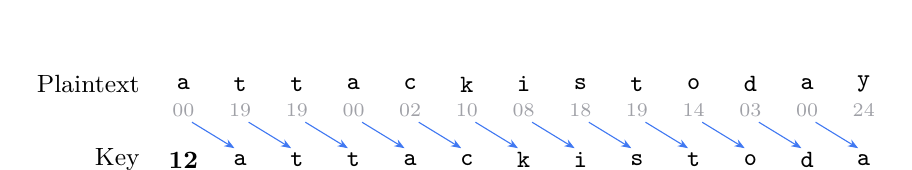
\begin{tikzpicture}[x=7.2mm,y=6mm,font=\small]
  \foreach \l/\v [count=\i] in {a/00,t/19,t/19,a/00,c/02,k/10,i/08,s/18,t/19,o/14,d/03,a/00,y/24}{
    \node (p\i) at (\i,0) {\ttx{\l}};
    \node[gray] at (\i,-0.55) {\scriptsize\v};
  }
  \node[anchor=east] at (0.4,0) {Plaintext};
  \node[anchor=east] at (0.4,-1.6) {Key};
  \node (k1) at (1,-1.6) {\textbf{12}};
  \foreach \l [count=\i] in {a,t,t,a,c,k,i,s,t,o,d,a}{
    \pgfmathtruncatemacro{\j}{\i+1}
    \node (k\j) at (\j,-1.6) {\ttx{\l}};
    \draw[-{Stealth[length=1.3mm]},acc] ($(p\i)+(0.15,-0.8)$) -- ($(k\j)+(-0.1,0.25)$);
  }
\end{tikzpicture}
\end{center}
\begin{center}\small\setlength{\tabcolsep}{3.6pt}
\begin{tabular}{@{}l*{13}{c}@{}}
\toprule
Plaintext & a&t&t&a&c&k&i&s&t&o&d&a&y\\
$P$ & 00&19&19&00&02&10&08&18&19&14&03&00&24\\
Key stream & \textbf{12}&00&19&19&00&02&10&08&18&19&14&03&00\\
$P + k$ & 12&19&\hl{38}&19&02&12&18&\hl{26}&\hl{37}&\hl{33}&17&03&24\\
$C$ & 12&19&12&19&02&12&18&00&11&07&17&03&24\\
Ciphertext & \textbf{M}&\textbf{T}&\textbf{M}&\textbf{T}&\textbf{C}&\textbf{M}&\textbf{S}&\textbf{A}&\textbf{L}&\textbf{H}&\textbf{R}&\textbf{D}&\textbf{Y}\\
\bottomrule
\end{tabular}
\end{center}
Ciphertext: \textbf{\ttx{MTMTCMSALHRDY}}. Each plaintext letter becomes the key one position later (arrows), and the last letter \ttx{y} keys nothing.

\textbf{Brute force.} Eve tries each $k_1$ and unrolls the chain $P_1 = C_1 - k_1$, $P_2 = C_2 - P_1$, \dots:
$k_1 = 11$ gives \ttx{bsuzdjjrunezz}, $k_1 = 13$ gives \ttx{zusbblhtspcbx}, and only $k_1 = 12$ gives readable text, \ttx{attackistoday}. At most 26 trials are needed.
\end{worked}

\subsection{Vernam cipher}
The autokey key is not independent of the message (it \emph{is} the message), so its statistics leak. The next step was taken by \textbf{Gilbert Vernam}, an AT\&T engineer, in \textbf{1918}: use a key stream \textbf{as long as the message} that \textbf{does not repeat} and has no statistical relationship to the plaintext, so that no pattern is left for a statistical attack. Vernam's cipher works on \textbf{binary bits}, not letters, because it was built for teletype machines that send each character as a short binary code. Each plaintext bit is combined with one key bit by exclusive-OR.

\begin{minipage}[c]{0.5\textwidth}
\[
C_i = P_i \oplus K_i \qquad\qquad P_i = C_i \oplus K_i
\]
Here $\oplus$ is XOR: the output is 1 if the two bits differ and 0 if they are equal. Decryption works because XOR undoes itself:
\[
C_i \oplus K_i = P_i \oplus K_i \oplus K_i = P_i \oplus 0 = P_i
\]
\end{minipage}\hfill
\begin{minipage}[c]{0.45\textwidth}
\centering\small
\begin{tabular}{cc|c}
\toprule
$a$ & $b$ & $a\oplus b$\\
\midrule
0&0&0\\ 0&1&1\\ 1&0&1\\ 1&1&0\\
\bottomrule
\end{tabular}
\qquad
\begin{tabular}{@{}r@{\;}l@{}}
$P$ & \ttx{1011}\\
$K$ & \ttx{0110}\\
\midrule
$C$ & \ttx{1101}\\
$C\oplus K$ & \ttx{1011} $= P$
\end{tabular}\\[2pt]
{\footnotesize (bit example is mine, not from the lecture)}
\end{minipage}

XOR is addition modulo 2, so Vernam is the Vigen\`ere idea applied to the two-letter alphabet $\{0, 1\}$: each key bit selects one of two ``Caesar ciphers'' (keep the bit, or flip it). XOR is the natural choice for two reasons. It is its own inverse, so the same operation and the same key stream encrypt and decrypt. And if a key bit is 0 or 1 with probability $\tfrac12$ each, independently of everything else, the ciphertext bit is also 0 or 1 with probability $\tfrac12$ whatever the plaintext bit is, so a single ciphertext bit reveals nothing about the plaintext bit.

\begin{center}
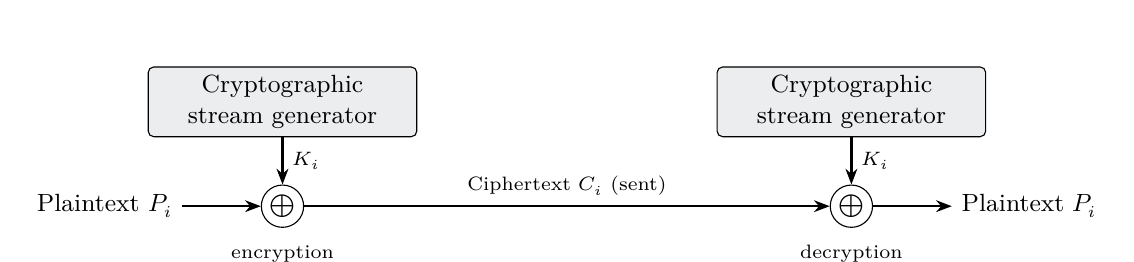
\begin{tikzpicture}[node distance=6mm]
  \node[box,fill=gray!15,text width=32mm] (g1) {Cryptographic stream generator};
  \node[draw,circle,below=6mm of g1,font=\large,inner sep=1pt] (x1) {$\oplus$};
  \node[left=10mm of x1,font=\small] (p1) {Plaintext $P_i$};
  \node[box,fill=gray!15,text width=32mm,right=38mm of g1] (g2) {Cryptographic stream generator};
  \node[draw,circle,below=6mm of g2,font=\large,inner sep=1pt] (x2) {$\oplus$};
  \node[right=10mm of x2,font=\small] (p2) {Plaintext $P_i$};
  \draw[arr] (g1) -- node[right,font=\scriptsize]{$K_i$} (x1);
  \draw[arr] (g2) -- node[right,font=\scriptsize]{$K_i$} (x2);
  \draw[arr] (p1) -- (x1);
  \draw[arr] (x1) -- node[above,font=\scriptsize]{Ciphertext $C_i$ (sent)} (x2);
  \draw[arr] (x2) -- (p2);
  \node[below=1mm of x1,font=\scriptsize] {encryption};
  \node[below=1mm of x2,font=\scriptsize] {decryption};
\end{tikzpicture}
\end{center}
Both sides need the \textbf{same, synchronised key stream}: the receiver's generator must produce exactly the bits the sender used, in the same order.

\textbf{Weakness.} Vernam's machine read the key from a \textbf{loop of paper tape}, so the key eventually \textbf{repeated}, and with enough ciphertext, and some known or probable plaintext, the cipher can be broken. The reason is that whenever two stretches of plaintext are encrypted with the same key bits, the key cancels: $C_1 \oplus C_2 = (P_1 \oplus K) \oplus (P_2 \oplus K) = P_1 \oplus P_2$. For example, with $P_1 = \ttx{10110010}$, $P_2 = \ttx{01100111}$ and $K = \ttx{11010100}$, the ciphertexts are $C_1 = \ttx{01100110}$ and $C_2 = \ttx{10110011}$, and $C_1 \oplus C_2 = \ttx{11010101} = P_1 \oplus P_2$, with no trace of $K$. The XOR of two English texts is full of structure; guessing a probable word in one plaintext reveals the matching part of the other, and then $K = C \oplus P$.
\textbf{Fix:} make the key truly random, as long as the message, and never reused. That is the \textbf{one-time pad} (\S\ref{sec:otp}), which gives perfect secrecy.

\subsection{The classical substitution ciphers compared}
Each cipher in this chapter was designed to remove the weakness that broke the one before it, and the summary below is the usual answer to a ``differentiate'' question.

\begin{mustknow}[: polyalphabetic ciphers]
\textbf{Vigen\`ere:} $C_i = (P_i + K_{i \bmod m}) \bmod 26$, keyword repeated; weakness: the period $m$ (Kasiski, then $m$ Caesar ciphers).
\textbf{Autokey:} key = keyword followed by the plaintext ($k_{i+m} = P_i$; Forouzan: $k_1$, then $k_i = P_{i-1}$); no period, but the key is English, and with a single $k_1$ only 26 keys; one plaintext change alters 2 ciphertext letters.
\textbf{Vernam (1918):} $C_i = P_i \oplus K_i$ on bits, key stream as long as the message; weakness: the tape loop repeats, and reused key bits cancel ($C_1 \oplus C_2 = P_1 \oplus P_2$). Random, never-reused key = one-time pad.
\end{mustknow}

\begin{center}\small\setlength{\tabcolsep}{4pt}
\begin{tabular}{@{}llllll@{}}
\toprule
Cipher & Unit & Key & Keys & Fixed substitute? & Main attack\\
\midrule
Shift (Caesar) & letter & shift $k$ & 25 & yes & brute force\\
Monoalphabetic & letter & permutation & $26!$ & yes & letter frequencies\\
Playfair & digram & $5\times5$ square & $25!$ & per digram & digram frequencies\\
Hill & $m$ letters & invertible $m\times m$ matrix & $< 26^{m^2}$ & per block & known plaintext\\
Vigen\`ere & letter & keyword, repeated & $26^m$ & no (period $m$) & Kasiski + Caesar\\
Autokey & letter & keyword + plaintext & $26^m$ & no (no period) & key is English\\
Vernam & bit & bit stream (tape) & -- & no & reused key stream\\
One-time pad & letter/bit & random, used once & -- & no & none (perfect)\\
\bottomrule
\end{tabular}
\end{center}

\begin{trap}[: the usual slips in Hill and Vigen\`ere answers]
In Hill, state the convention ($C = PK$ with row vectors, or $C = KP$ with columns) and keep it for decryption; check $\gcd(\det K, 26) = 1$ \emph{before} computing the inverse; turn negative entries into $0$--$25$ by adding 26; and always verify $KK^{-1} \equiv I$. In the known-plaintext attack the inverse goes on the left: $K = P^{-1}C$. In Vigen\`ere, remove the spaces first so the keyword runs continuously across words; in autokey, decrypt strictly left to right.
\end{trap}

\begin{fixbox}
\begin{itemize}
  \item The notes put ``key and plaintext share letter frequencies'' under Vigen\`ere cryptanalysis. That point is really about the autokey system, where the key \emph{is} plaintext, so it is placed there above.
  \item Slide L5 (autokey) is correct: \ttx{attackistoday} with $k_1 = 12$ gives \ttx{MTMTCMSALHRDY}; slide L5 (Vigen\`ere, PASCAL) is correct: \ttx{HHWKSWXSLGNTCG} (both checked by script).
\end{itemize}
\end{fixbox}

% Sources: Neso videos (one-time pad, rail fence, row-column transposition; notes5.md), college Lecture 5 slides 54-55,
% Stallings 2.2-2.3, Forouzan 3.2. Every number recomputed by script (scratchpad/r3/verify.py).
\providecommand{\railfence}[1]{%
  \foreach \l/\r [count=\i] in {#1}{\node[font=\small] (rf\i) at (\i*0.5,-\r*0.6) {\l};}}

\section{One-Time Pad \hot}\label{sec:otp}
\asked{Mid-sem 2025--26 Q1 (8 marks): OTP-Vigen\`ere with key stream 9 0 1 7 23 15 21 14 11 11 2 8 9 (Stallings 2.x). Part (b), finding a key that maps the ciphertext to another plaintext, is exactly why an OTP is unbreakable: every plaintext of the same length is possible.}

\subsection{How it grew out of the earlier ciphers}
Every substitution cipher so far was broken through the same flaw: the key is reused, so some regularity of the plaintext survives into the ciphertext. A monoalphabetic cipher applies one fixed substitution to the whole message, so the letter frequencies of English pass straight through. Vigen\`ere rotates through $m$ substitutions, so once $m$ is known the ciphertext splits into $m$ interleaved Caesar ciphers (\S\ref{sec:classextra} shows how the Kasiski test finds $m$). The autokey cipher removes the period by continuing the key with the plaintext itself, but then the key is English text and carries English statistics. Vernam's cipher (1918) works on bits with a long key stream punched on paper tape, but the tape was a loop, so the key eventually repeated and a long enough message could be broken.

Shannon's study of secrecy showed what the key must look like for \emph{no} regularity to survive: each plaintext symbol must be encrypted with a key symbol chosen \textbf{at random from the whole key domain}, independently of every other symbol. Even the weak additive cipher becomes perfect under this rule. It is broken easily because the same shift is used for every letter; but if the first letter is shifted by 04, the second by 02, the third by 21, and each shift is drawn at random from $00, 01, \dots, 25$, then nothing links one ciphertext letter to another or to the plaintext. This is the \textbf{one-time pad} (OTP), the last substitution technique of the course and an improvement to the Vernam cipher (Stallings credits the improvement to Joseph Mauborgne; Forouzan's slides credit Vernam).

\begin{center}\small
\begin{tabularx}{\textwidth}{@{}l X X@{}}
\toprule
Cipher & Key & What goes wrong\\
\midrule
Vigen\`ere & short keyword, \textbf{repeated} & repeats every $m$ letters $\Rightarrow$ split into Caesar ciphers\\
Autokey & keyword + plaintext & key is English $\Rightarrow$ has English letter frequencies\\
Vernam & long key stream (paper tape) & tape loops, so the key \textbf{eventually repeats}\\
\textbf{One-time pad} & \textbf{truly random}, \textbf{same length} as message, \textbf{used once} & nothing to exploit\\
\bottomrule
\end{tabularx}
\end{center}

\subsection{Definition and mechanism}
In a one-time pad the key is a \textbf{truly random} sequence that is \textbf{as long as the message}, so it never has to be repeated. The key is used to encrypt and decrypt \textbf{a single message} and is then \textbf{discarded}; every new message needs a new random key of its own length. The encryption rule itself is unchanged from Vigen\`ere (letters) or Vernam (bits): only the key is different. Stallings calls the result ``the ultimate in security'', because such a scheme is unbreakable.

\begin{mustknow}[: one-time pad]
\textbf{Key}: truly random, same length as the message, used once, then destroyed.\\[2pt]
\textbf{Letters}: $C_i = (P_i + K_i) \bmod 26$, \;$P_i = (C_i - K_i) \bmod 26$. \qquad \textbf{Bits}: $C_i = P_i \oplus K_i$, \;$P_i = C_i \oplus K_i$.\\[2pt]
\textbf{Perfect secrecy}: $\Pr[M \mid C] = \Pr[M]$; the ciphertext reveals nothing about the plaintext. The OTP is the \emph{only} cipher with this property (key at least as long as the message is necessary).\\[2pt]
\textbf{Two difficulties}: (1) making large quantities of random keys; (2) key distribution and protection.
\end{mustknow}

Decryption recovers the plaintext because the key cancels: $(P_i + K_i) - K_i \equiv P_i \pmod{26}$, and $(P_i \oplus K_i) \oplus K_i = P_i \oplus 0 = P_i$, since XOR of a bit with itself is 0. The receiver therefore needs exactly the same key, in the same order, aligned with the same letter positions; this requirement is the source of all the practical difficulties discussed below.

\subsection{Example 1: letters}
Plaintext \ttx{attackatdawn}, random key \ttx{qvhzmxkbplwe} (12 key letters for 12 plaintext letters). Each letter is shifted by its own key value, and four sums pass 25 and wrap:
\begin{center}\small\setlength{\tabcolsep}{4.5pt}
\begin{tabular}{@{}l*{12}{c}@{}}
\toprule
Plain & a&t&t&a&c&k&a&t&d&a&w&n\\
$P$ & 0&19&19&0&2&10&0&19&3&0&22&13\\
Key & q&v&h&z&m&x&k&b&p&l&w&e\\
$K$ & 16&21&7&25&12&23&10&1&15&11&22&4\\
$P+K$ & 16&\hl{40}&\hl{26}&25&14&\hl{33}&10&20&18&11&\hl{44}&17\\
$\bmod 26$ & 16&14&0&25&14&7&10&20&18&11&18&17\\
Cipher & \textbf{Q}&\textbf{O}&\textbf{A}&\textbf{Z}&\textbf{O}&\textbf{H}&\textbf{K}&\textbf{U}&\textbf{S}&\textbf{L}&\textbf{S}&\textbf{R}\\
\bottomrule
\end{tabular}
\end{center}
Ciphertext \textbf{\ttx{QOAZOHKUSLSR}}. The receiver computes $(C - K) \bmod 26$ letter by letter to get \ttx{attackatdawn} back, then destroys the key. The two \ttx{t}'s of \ttx{att} became \ttx{O} and \ttx{A}, and the two \ttx{S}'s of the ciphertext came from different letters (\ttx{d} and \ttx{w}): equal letters do not produce equal letters, and equal ciphertext letters do not mean equal plaintext letters.

\subsection{Example 2: bits}
``HI'' in 8-bit ASCII, XORed with a random 16-bit key. Each ciphertext bit is 1 exactly where the plaintext bit and the key bit differ:
\begin{center}\small\ttfamily
\begin{tabular}{@{}r@{\quad}l@{\quad}l@{}}
\rmfamily Plaintext (H, I) & 01001000 & 01001001\\
\rmfamily Key & 10110101 & 01101100\\
\midrule
\rmfamily Ciphertext $P\oplus K$ & 11111101 & 00100101\\
\rmfamily $C \oplus K$ & 01001000 & 01001001 \rmfamily\;= ``HI'' again\\
\end{tabular}
\end{center}

\subsection{Why it cannot be broken}
The one-time pad produces random output that has \textbf{no statistical relationship to the plaintext}. Since the ciphertext contains no information whatsoever about the plaintext, there is simply no way to break the code, and the security of the scheme comes \textbf{entirely from the randomness of the key}. This can be seen at three levels.

\textbf{One letter.} Suppose the attacker sees the ciphertext letter \ttx{Q} ($= 16$). Every plaintext letter could have produced it, each with exactly one key letter, namely $K = (16 - P) \bmod 26$:
\begin{center}\small\setlength{\tabcolsep}{5pt}
\begin{tabular}{@{}l*{7}{c}@{}}
\toprule
If the plaintext was & a & b & c & d & e & \dots & z\\
then the key was & q & p & o & n & m & \dots & r\\
\bottomrule
\end{tabular}
\end{center}
Since the key letter was drawn at random, all 26 cases are \textbf{equally likely}, and seeing \ttx{Q} tells the attacker nothing. The same argument shows that the ciphertext letters themselves are uniformly distributed: $\Pr[C_i = c] = \sum_p \Pr[P_i = p] \cdot \Pr[K_i = c - p] = \sum_p \Pr[P_i = p] \cdot \tfrac{1}{26} = \tfrac{1}{26}$, whatever the plaintext statistics. The ciphertext has a flat frequency histogram (no peak for \ttx{e} to aim at), and since the key never repeats, the Kasiski and index-of-coincidence tests of \S\ref{sec:classextra} find nothing.

\textbf{The whole message.} For a message of $n$ letters there are $26^n$ keys, exactly as many as there are $n$-letter strings, and every string is the decryption of the ciphertext under exactly one key. The same ciphertext therefore decrypts to anything of the same length:
\begin{center}\small
\begin{tabular}{@{}lll@{}}
\toprule
Ciphertext & Key tried & Result\\
\midrule
\ttx{QOAZOHKUSLSR} & \ttx{qvhzmxkbplwe} & \textbf{attack at dawn}\\
\ttx{QOAZOHKUSLSR} & \ttx{zkhikhruztku} & \textbf{retreat at six}\\
\ttx{KXFUDM} & \ttx{kemubc} & \textbf{attack}\\
\ttx{KXFUDM} & \ttx{htaqqj} & \textbf{defend}\\
\bottomrule
\end{tabular}
\end{center}
A brute-force search produces \emph{every} meaningful message of that length, with nothing to say which one was sent. Compare the Caesar cipher, where only one of the 25 tries makes sense (GERMANY): there the key space is far smaller than the message space, so wrong keys give gibberish and the right one stands out.

\subsection{Perfect secrecy: the derivation}
\textbf{Definition (Shannon, 1949).} A cipher has \textbf{perfect secrecy} if, for every plaintext $M$ and every ciphertext $C$ that can occur,
\[
\Pr[M \mid C] = \Pr[M].
\]
$\Pr[M]$ is what the attacker believes about the message before interception (for example, that ``no attack today'' is the usual message), and $\Pr[M \mid C]$ is what she believes after seeing $C$. Equality means the ciphertext changes nothing: \imp{given a ciphertext from a perfectly secure cipher, absolutely nothing is revealed about the plaintext.}

\textbf{The one-time pad meets the definition.} Fix any plaintext $M$ and ciphertext $C$ of length $n$. Exactly one key maps $M$ to $C$, namely $K = C - M \pmod{26}$ letter by letter (or $K = C \oplus M$ for bits). Every key is equally likely, with probability $1/26^n$, so
\[
\Pr[C \mid M] = \Pr[K = C - M] = \frac{1}{26^n}\quad\text{for every } M .
\]
Averaging over the messages, $\Pr[C] = \sum_{M} \Pr[M]\Pr[C \mid M] = \frac{1}{26^n}\sum_M \Pr[M] = \frac{1}{26^n}$. Bayes' rule then gives
\[
\Pr[M \mid C] = \frac{\Pr[C \mid M]\,\Pr[M]}{\Pr[C]} = \frac{(1/26^n)\,\Pr[M]}{1/26^n} = \Pr[M].
\]
In words: every key is equally likely, and for each candidate plaintext exactly one key turns it into the observed $C$, so $C$ ``points'' equally strongly to every plaintext, and the attacker's probabilities stay where they were. For a one-bit pad with $\Pr[M = 0] = 0.9$: $\Pr[C = 1] = 0.9 \cdot 0.5 + 0.1 \cdot 0.5 = 0.5$, and $\Pr[M = 0 \mid C = 1] = 0.5 \cdot 0.9 / 0.5 = 0.9$; Eve's best guess after interception is exactly her guess before it.

\textbf{Why the key must be as long as the message.} Suppose there were fewer keys than possible messages. Decrypting a given $C$ under all keys yields at most as many candidate plaintexts as there are keys, so some message $M$ with $\Pr[M] > 0$ is not among them and has $\Pr[M \mid C] = 0$: the ciphertext has ruled it out, and secrecy is not perfect. For example, a Caesar shift used for a two-letter message cannot turn \ttx{aa} into \ttx{AB}, because one shift maps equal letters to equal letters; seeing \ttx{AB} eliminates \ttx{aa}, \ttx{bb}, \dots. Hence perfect secrecy needs at least as many keys as messages, i.e.\ at least as much random key as message. This is Shannon's bound, and it is the reason the OTP is the \textbf{only} practical cipher with perfect secrecy.

\textbf{Unconditional versus computational security.} Perfect secrecy is the \textbf{unconditionally secure} case of \S\ref{sec:schemes}: no amount of ciphertext or computing power helps, because the information is simply not there. Every other cipher in this course (DES, AES, RSA, \dots) is only \textbf{computationally} secure: it can be broken in principle, but doing so costs more time or money than the information is worth.

\begin{trap}[: what perfect secrecy does not give]
The OTP hides the \emph{content} among messages of the \emph{same length}; it does not hide the length (if Alice's answer is ``YES'' or ``NO'', a 3-letter ciphertext gives it away). It also gives no integrity: flipping a ciphertext bit flips the same plaintext bit, and Bob cannot detect it. Integrity needs a hash or MAC (\S\ref{sec:integrity}).
\end{trap}

\subsection{The rules, and what breaks if you bend them}
\textbf{Rule 1: never reuse a key (the ``two-time pad'').} Encrypt a second message \ttx{holdposition} with the \emph{same} key \ttx{qvhzmxkbplwe}; the result is $C_2 = $ \ttx{XJSCBLCJITKR}. Subtracting the two ciphertexts cancels the key,
\[
C_1 - C_2 = (P_1 + K) - (P_2 + K) = P_1 - P_2 \pmod{26},
\]
and indeed both differences equal \ttx{TFIXNWILKSIA}. What remains is two English texts combined with each other, which has strong structure (common words, frequent letters) that the attacker can attack without knowing any key. Worse, if the attacker knows or guesses $P_1$ (``attack at dawn'' is a stock phrase), she recovers the key $K = C_1 - P_1 = $ \ttx{qvhzmxkbplwe} and then $P_2 = C_2 - K = $ \textbf{hold position}. With bits the same cancellation is $C_1 \oplus C_2 = P_1 \oplus P_2$. Historically, Soviet pads that were reused in the 1940s were partly read by the US VENONA project for exactly this reason.

\textbf{Rule 2: the key must be truly random.} If the key is text taken from a book (a \textbf{running key}), it has English letter frequencies and can be attacked like the autokey. If it is generated by a formula from a short seed, the cipher is really a stream cipher: at best \emph{computationally} secure, never perfect, because the number of possible key streams is only the number of seeds.

\textbf{Rule 3: the key must be at least as long as the message.} A shorter key has to repeat, and then the cipher is back to Vigen\`ere or Vernam with their weaknesses; the derivation above shows that perfect secrecy is then impossible.

\textbf{Known plaintext does not hurt a correctly used OTP.} If the attacker learns one plaintext and its ciphertext, she gets $K = C - P$, but only for that message, and that key is never used again. For every other cipher a known pair helps break future traffic (\S\ref{sec:classextra}); here it is worthless.

\subsection{Two fundamental difficulties}
In theory the one-time pad is the end of the story; in practice it has two fundamental difficulties.
\begin{enumerate}[leftmargin=1.5em]
  \item \imp{The practical problem of making large quantities of random keys.} Every message needs fresh random key material of the same size, so a system carrying a lot of traffic needs millions of truly random characters on a regular basis. Pseudorandom generators do not qualify (Rule 2), and good physical sources of randomness are slow.
  \item \imp{Even more daunting is the problem of key distribution and protection.} For every message, sender and receiver must hold an identical key of the same length, delivered and stored securely, and destroyed after use. If a secure channel able to carry that much key existed, the message could simply be sent over it instead.
\end{enumerate}
The second point is softened by \emph{timing}: the key can be carried in advance, by a trusted courier, at a moment and by a route the parties choose, after which the messages can travel over any insecure channel. The slide's example is a president who sends a trusted envoy with a random key to another president before sending a completely secret message. This is why Forouzan calls the OTP ``a perfect cipher, but almost impossible to implement commercially''.

\textbf{Advantages.} Perfect secrecy: no attack, however much ciphertext or computing power the attacker has, can extract information about the plaintext. Encryption and decryption are trivial additions or XORs. \textbf{Disadvantages.} The key is as long as all the traffic ever sent, must be truly random, must reach the receiver securely in advance and must never be reused; it gives no integrity. Because of these difficulties, \imp{the one-time pad is of limited utility, and is useful primarily for low-bandwidth channels requiring very high security} (diplomatic and military links).

\subsection{Exam-format one-time-pad numerical}
\begin{worked}[: Stallings 2.x, mid-sem 2025--26 Q1]
\textbf{Q.} This problem uses a one-time pad version of the Vigen\`ere cipher: each plaintext letter is shifted by the next number of the key stream \ttx{9 0 1 7 23 15 21 14 11 11 2 8 9}. (a) Encrypt \ttx{sendmoremoney}. (b) Using the ciphertext from (a), find a key stream that makes it decrypt to \ttx{cashnotneeded}. (8 marks)

\textbf{(a)} $C_i = (P_i + K_i) \bmod 26$, letters numbered from $a = 0$:
\begin{center}\small\setlength{\tabcolsep}{4pt}
\begin{tabular}{@{}l*{13}{c}@{}}
\toprule
Plain & s&e&n&d&m&o&r&e&m&o&n&e&y\\
$P$ & 18&4&13&3&12&14&17&4&12&14&13&4&24\\
$K$ & 9&0&1&7&23&15&21&14&11&11&2&8&9\\
$P{+}K$ & \hl{27}&4&14&10&\hl{35}&\hl{29}&\hl{38}&18&23&25&15&12&\hl{33}\\
mod 26 & 1&4&14&10&9&3&12&18&23&25&15&12&7\\
Cipher & \textbf{B}&\textbf{E}&\textbf{O}&\textbf{K}&\textbf{J}&\textbf{D}&\textbf{M}&\textbf{S}&\textbf{X}&\textbf{Z}&\textbf{P}&\textbf{M}&\textbf{H}\\
\bottomrule
\end{tabular}
\end{center}
Ciphertext: \textbf{\ttx{BEOKJDMSXZPMH}}.

\textbf{(b)} The key that turns $C$ into a chosen plaintext $P'$ is $K'_i = (C_i - P'_i) \bmod 26$:
\begin{center}\small\setlength{\tabcolsep}{3.6pt}
\begin{tabular}{@{}l*{13}{c}@{}}
\toprule
$C$ & B 1&E 4&O 14&K 10&J 9&D 3&M 12&S 18&X 23&Z 25&P 15&M 12&H 7\\
$P'$ & c 2&a 0&s 18&h 7&n 13&o 14&t 19&n 13&e 4&e 4&d 3&e 4&d 3\\
$C - P'$ & $-1$&4&$-4$&3&$-4$&$-11$&$-7$&5&19&21&12&8&4\\
$K'$ & \textbf{25}&\textbf{4}&\textbf{22}&\textbf{3}&\textbf{22}&\textbf{15}&\textbf{19}&\textbf{5}&\textbf{19}&\textbf{21}&\textbf{12}&\textbf{8}&\textbf{4}\\
\bottomrule
\end{tabular}
\end{center}
Key stream: \textbf{25 4 22 3 22 15 19 5 19 21 12 8 4}. Check, first letter: $(2 + 25) \bmod 26 = 1 = $ \ttx{B} \checkmark.

\textbf{Conclusion to write.} The same ciphertext decrypts to \ttx{sendmoremoney} under one key and to \ttx{cashnotneeded} under another, and both keys are equally likely random streams. An attacker who tries all keys gets every 13-letter message and cannot tell which was sent, so the one-time pad cannot be broken by brute force: it has perfect secrecy.
\end{worked}

\section{Transposition Ciphers}\label{sec:transp}
Substitution ciphers replace letters, and every one of them up to the one-time pad was attacked through the statistics of the replaced letters. A \textbf{transposition cipher} takes the opposite approach: some sort of \textbf{permutation is applied to the plaintext letters}. The letters themselves are \textbf{not replaced}; only their \textbf{positions} change, so a symbol in the first position of the plaintext may appear in the tenth position of the ciphertext. A \textbf{permutation} of $n$ positions is a rearrangement in which every position receives exactly one letter; there are $n!$ of them, and the key of a transposition cipher is a permutation or a rule (depth, column order) that generates one.

\textbf{Why transposition keeps the letter frequencies.} Every plaintext letter appears in the ciphertext exactly once, merely at another position, so the ciphertext is an \emph{anagram} of the plaintext: the two contain the same letters the same number of times, and their single-letter frequencies are identical. (Script check: the ciphertext of the Kill Corona example below has exactly the letter counts of its padded plaintext.) This gives the cryptanalyst an immediate test. If a ciphertext is unreadable but its letter counts look like normal English (\ttx{e} about 12.7\%, \ttx{t} 9.1\%, \ttx{a} 8.2\%, and \ttx{j}, \ttx{q}, \ttx{x}, \ttx{z} almost absent), the letters are genuine and only their order is scrambled: the cipher is a \textbf{transposition}. A monoalphabetic substitution shows the same \emph{shape} of histogram but on the wrong letters (the tallest bar is not \ttx{e}), and a polyalphabetic cipher flattens it. The frequency count identifies a transposition but does not break it; the attacker still has to find the order, using digram statistics (\ttx{th}, \ttx{he}, \ttx{in}, \dots) to decide which letters belong next to each other. The simplest transposition is the rail fence.

\begin{mustknow}[: transposition]
Substitution changes the \emph{letters}; transposition changes their \emph{positions}, so \textbf{letter frequencies are preserved} (a frequency count that looks like plain English means transposition).\\
Rail fence, depth $D$: zig-zag with period $2(D-1)$, read row by row. Row--column: write row by row, read column by column, \textbf{key = order of the columns}; two stages = do it again on the ciphertext.
\end{mustknow}

\subsection{Rail fence}
In the rail fence technique the plaintext is \textbf{written down as a sequence of diagonals and then read off as a sequence of rows}. The letters are written on $D$ rows (the \textbf{depth}), moving down one row per letter from row 1 to row $D$ and then back up to row 1, in a zig-zag; spaces and punctuation are dropped. The ciphertext is row 1, followed by row 2, and so on. Going down takes $D - 1$ steps and coming back takes $D - 1$ steps, so the row pattern repeats every $2(D-1)$ letters.

\textbf{Example:} ``neso academy is the best'', depth 2 (20 letters):
\begin{center}
\begin{tikzpicture}
  \railfence{n/0,e/1,s/0,o/1,a/0,c/1,a/0,d/1,e/0,m/1,y/0,i/1,s/0,t/1,h/0,e/1,b/0,e/1,s/0,t/1}
  \foreach \i in {1,...,19}{\pgfmathtruncatemacro{\j}{\i+1}\draw[gray!50] (rf\i) -- (rf\j);}
  \node[font=\scriptsize,anchor=east] at (0.2,0) {row 1};
  \node[font=\scriptsize,anchor=east] at (0.2,-0.6) {row 2};
\end{tikzpicture}
\end{center}
Row 1: \ttx{NSAAEYSHBS}\quad Row 2: \ttx{EOCDMITEET}\quad $\Rightarrow$\quad \textbf{\ttx{NSAAEYSHBSEOCDMITEET}}

\textbf{Depth 3}, ``Thank you very much'' (16 letters). The path visits rows 1, 2, 3, 2, 1, 2, 3, \dots\ and repeats every $2(D-1) = 4$ letters:
\begin{center}
\begin{tikzpicture}
  \railfence{t/0,h/1,a/2,n/1,k/0,y/1,o/2,u/1,v/0,e/1,r/2,y/1,m/0,u/1,c/2,h/1}
  \foreach \i in {1,...,15}{\pgfmathtruncatemacro{\j}{\i+1}\draw[gray!50] (rf\i) -- (rf\j);}
\end{tikzpicture}
\end{center}
Rows: \ttx{TKVM} + \ttx{HNYUEYUH} + \ttx{AORC} $\Rightarrow$ \textbf{\ttx{TKVMHNYUEYUHAORC}}. The middle row holds twice as many letters as the outer rows, because the zig-zag passes through it on the way down and again on the way up.

\textbf{Homework} (``neso academy is the best'', depth 3): the rows are \ttx{NAESB}, \ttx{EOCDMITEET} and \ttx{SAYHS}, so the ciphertext is \textbf{\ttx{NAESBEOCDMITEETSAYHS}}.

\textbf{Security.} The only secret is the depth, and it can only be one of $2, 3, \dots, L - 1$ for an $L$-letter message, so an attacker simply tries every depth; the frequencies are English, which tells her at once that she is facing a transposition. The rail fence is therefore a scrambling rule rather than a real cipher (Forouzan files it under \emph{keyless} transpositions, \S\ref{sec:classextra}).

\subsection{Decrypting a rail fence}
The receiver knows the depth $D$. The difficulty is that the ciphertext does not show where one row ends and the next begins, so the first job is to work out \textbf{how many letters each row holds}; after that the zig-zag can be rebuilt and read along its path.
\begin{enumerate}[leftmargin=1.5em]
  \item Count the letters $L$. The zig-zag pattern of rows repeats every $2(D-1)$ letters.
  \item Write the \textbf{row number of every position} (1, 2, \dots, $D$, \dots, 2, 1, 2, \dots) and \textbf{count} how many times each row appears.
  \item \textbf{Cut} the ciphertext into pieces of those lengths: the first piece is row 1, the next is row 2, and so on.
  \item Put each piece back into its row's positions, left to right. Then \textbf{read along the zig-zag} (position 1, 2, 3, \dots).
\end{enumerate}
\textbf{The counts without writing the pattern.} Write $L = q \cdot 2(D-1) + r$ with $0 \le r < 2(D-1)$. Each complete cycle visits row 1 and row $D$ once and every middle row twice, and within a cycle row $i$ is visited at positions $i$ and $2D - i$. So row 1 holds $q + [r \ge 1]$ letters, row $D$ holds $q + [r \ge D]$, and a middle row $i$ holds $2q + [r \ge i] + [r \ge 2D - i]$, where $[\cdot]$ is 1 if the condition holds and 0 otherwise. For $L = 17$, $D = 4$: $17 = 2 \cdot 6 + 5$, giving $3, 5, 6, 3$, as in Example 3 below.

\textbf{Example 1: depth 2.} \ttx{NSAAEYSHBSEOCDMITEET} (20 letters). The pattern is 1 2 1 2 \dots, so each row has 10 letters:
row 1 $=$ \ttx{NSAAEYSHBS}, row 2 $=$ \ttx{EOCDMITEET}. Take letters alternately from row 1 and row 2:
\ttx{N}\textbf{\ttx{E}}\ttx{S}\textbf{\ttx{O}}\ttx{A}\textbf{\ttx{C}}\dots\ $\Rightarrow$ \textbf{nesoacademyisthebest}.
(Depth-2 shortcut: split in half and interleave. With an odd length, row 1 gets the extra letter.)

\textbf{Example 2: depth 3.} \ttx{TKVMHNYUEYUHAORC} (16 letters). The pattern repeats every $2(3-1) = 4$:
\begin{center}\small\setlength{\tabcolsep}{4pt}
\begin{tabular}{@{}l*{16}{c}@{}}
\toprule
Position & 1&2&3&4&5&6&7&8&9&10&11&12&13&14&15&16\\
Row & 1&2&3&2&1&2&3&2&1&2&3&2&1&2&3&2\\
\bottomrule
\end{tabular}
\end{center}
Row 1 appears 4 times, row 2 8 times, row 3 4 times. Cut: \ttx{TKVM | HNYUEYUH | AORC}.
Fill the row-1 positions (1, 5, 9, 13) with T K V M, the row-2 positions with H N Y U E Y U H, and the row-3 positions with A O R C. Reading positions 1 to 16 gives \textbf{thankyouverymuch}.

\textbf{Example 3: depth 4, unequal rows} (the tricky case). \ttx{CGIRORYSYTAHFNPPU} (17 letters). The pattern repeats every $2(4-1) = 6$:
\begin{center}\small\setlength{\tabcolsep}{4pt}
\begin{tabular}{@{}l*{17}{c}@{}}
\toprule
Position & 1&2&3&4&5&6&7&8&9&10&11&12&13&14&15&16&17\\
Row & 1&2&3&4&3&2&1&2&3&4&3&2&1&2&3&4&3\\
\bottomrule
\end{tabular}
\end{center}
Counts: row 1 $= 3$, row 2 $= 5$, row 3 $= 6$, row 4 $= 3$ (total 17 \checkmark). Cut: \ttx{CGI | RORYS | YTAHFN | PPU}. Put the pieces back:
\begin{center}
\begin{tikzpicture}
  \railfence{C/0,R/1,Y/2,P/3,T/2,O/1,G/0,R/1,A/2,P/3,H/2,Y/1,I/0,S/1,F/2,U/3,N/2}
  \foreach \i in {1,...,16}{\pgfmathtruncatemacro{\j}{\i+1}\draw[gray!50] (rf\i) -- (rf\j);}
  \node[font=\scriptsize,anchor=east] at (0.2,0) {row 1: CGI};
  \node[font=\scriptsize,anchor=east] at (0.2,-0.6) {row 2: RORYS};
  \node[font=\scriptsize,anchor=east] at (0.2,-1.2) {row 3: YTAHFN};
  \node[font=\scriptsize,anchor=east] at (0.2,-1.8) {row 4: PPU};
\end{tikzpicture}
\end{center}
Read along the line: \textbf{cryptographyisfun} (``cryptography is fun''). The same steps, with row counts 5, 10, 5, turn the homework answer above back into \ttx{nesoacademyisthebest}.

\begin{trap}[: unequal rows]
Do not assume the rows are equal, or that the middle rows are equal to each other. In Example 3 rows 2 and 3 have different lengths (5 and 6) because the message stops partway through a cycle, after the zig-zag has passed row 3 on its way up but before it reaches row 2.
\end{trap}

\subsection{Row--column transposition}
The rail fence has too few keys to be of any use. A more complex scheme uses a \textbf{rectangle}: the message is \textbf{written row by row} into a rectangle of $c$ columns and \textbf{read column by column}, but the columns are read in a \textbf{secret order}. The \textbf{key} is that order of the columns, written as a number above each column (the column marked 1 is read first). Leftover cells in the last row are filled with agreed filler letters (\ttx{x}, \ttx{y}, \ttx{z}), so that every column has the same height and the receiver can remove the fillers after decryption.

\textbf{Example:} ``Kill Corona Virus at twelve am tomorrow'' (33 letters), 7 columns $\times$ 5 rows = 35 cells, so 2 fillers (\ttx{y}, \ttx{z}). Key \textbf{4 3 1 2 5 6 7}.
\begin{center}\small
\begin{minipage}[c]{0.4\textwidth}\centering
\begin{tabular}{|*{7}{c|}}
\multicolumn{1}{c}{4}&\multicolumn{1}{c}{3}&\multicolumn{1}{c}{\textbf{1}}&\multicolumn{1}{c}{2}&\multicolumn{1}{c}{5}&\multicolumn{1}{c}{6}&\multicolumn{1}{c}{7}\\
\hline
k&i&\cellcolor{warn!18}l&l&c&o&r\\ \hline
o&n&\cellcolor{warn!18}a&v&i&r&u\\ \hline
s&a&\cellcolor{warn!18}t&t&w&e&l\\ \hline
v&e&\cellcolor{warn!18}a&m&t&o&m\\ \hline
o&r&\cellcolor{warn!18}r&o&w&\textit{y}&\textit{z}\\ \hline
\end{tabular}\\[2pt]
{\footnotesize numbers above = read order}
\end{minipage}
\begin{minipage}[c]{0.5\textwidth}
\begin{tabular}{@{}lll@{}}
\toprule
Order & Column & Letters\\
\midrule
1 & col 3 & LATAR\\
2 & col 4 & LVTMO\\
3 & col 2 & INAER\\
4 & col 1 & KOSVO\\
5 & col 5 & CIWTW\\
6 & col 6 & OREOY\\
7 & col 7 & RULMZ\\
\bottomrule
\end{tabular}
\end{minipage}
\end{center}
Answer: \textbf{\ttx{LATARLVTMOINAERKOSVOCIWTWOREOYRULMZ}}

\textbf{Key space and weakness.} With $c$ columns there are $c!$ reading orders ($7! = 5040$ here), multiplied by the choice of $c$, so brute force by hand is already tedious. The weakness is structural. Consecutive ciphertext letters come from one column, i.e.\ from plaintext positions exactly $c$ apart: the first five ciphertext letters are plaintext letters 3, 10, 17, 24, 31. An attacker who guesses the number of rows (here 5, a divisor of 35) cuts the ciphertext into 5-letter pieces, stands them side by side as columns and rearranges the columns until the rows read as English, guided by common digrams; Forouzan calls this the \textbf{pattern attack} (\S\ref{sec:classextra}). This is why the lecture says a single transposition ``can be reconstructed''.

\begin{worked}[: decrypting a row--column transposition]
\textbf{Q.} Decrypt \ttx{LATARLVTMOINAERKOSVOCIWTWOREOYRULMZ}, written row by row into 7 columns and read in the column order \textbf{4 3 1 2 5 6 7}.

\textbf{Column height.} $L = 35$ letters in 7 columns, so every column holds $35 / 7 = 5$ letters (5 rows).

\textbf{Refill the columns in key order.} The first 5 letters belong to the column numbered 1 (column 3), the next 5 to the column numbered 2 (column 4), and so on:
\begin{center}\small
\begin{tabular}{@{}llllllll@{}}
\toprule
Piece & LATAR & LVTMO & INAER & KOSVO & CIWTW & OREOY & RULMZ\\
Goes to column & 3 & 4 & 2 & 1 & 5 & 6 & 7\\
\bottomrule
\end{tabular}
\end{center}
\textbf{Read row by row.} Column 1 is now \ttx{KOSVO}, column 2 \ttx{INAER}, column 3 \ttx{LATAR}, and so on; reading the rebuilt grid across its rows gives \ttx{killcor | onaviru | sattwel | veamtom | orrowyz}. Removing the fillers \ttx{yz}, the plaintext is \textbf{kill corona virus at twelve am tomorrow}. Check: re-encrypting gives the received ciphertext \checkmark.
\end{worked}

\subsection{Two stages: more complex}
A single transposition leaves the regular pattern just described. The remedy is to \textbf{feed the ciphertext back in} and transpose again, usually with the same key:
\begin{center}\small
\begin{minipage}[c]{0.4\textwidth}\centering
\begin{tabular}{|*{7}{c|}}
\multicolumn{1}{c}{4}&\multicolumn{1}{c}{3}&\multicolumn{1}{c}{\textbf{1}}&\multicolumn{1}{c}{2}&\multicolumn{1}{c}{5}&\multicolumn{1}{c}{6}&\multicolumn{1}{c}{7}\\
\hline
L&A&\cellcolor{warn!18}T&A&R&L&V\\ \hline
T&M&\cellcolor{warn!18}O&I&N&A&E\\ \hline
R&K&\cellcolor{warn!18}O&S&V&O&C\\ \hline
I&W&\cellcolor{warn!18}T&W&O&R&E\\ \hline
O&Y&\cellcolor{warn!18}R&U&L&M&Z\\ \hline
\end{tabular}
\end{minipage}
\begin{minipage}[c]{0.5\textwidth}
Read columns 3, 4, 2, 1, 5, 6, 7:\\[2pt]
\ttx{TOOTR AISWU AMKWY LTRIO RNVOL LAORM VECEZ}
\end{minipage}
\end{center}
Answer: \textbf{\ttx{TOOTRAISWUAMKWYLTRIORNVOLLAORMVECEZ}}.
The full key is now: the rectangle size, the column order and the number of stages. To decrypt, the receiver applies the single-stage decryption of the worked example twice (the second stage is undone first).

\textbf{Why two stages are stronger.} After one stage, ciphertext positions 1--5 hold plaintext letters $3, 10, 17, 24, 31$: a run with constant step 7. After two stages they hold plaintext letters $17, 32, 8, 26, 7$ (computed by composing the two permutations), and no constant step appears anywhere in the ciphertext. Cutting the ciphertext into columns therefore no longer produces fragments of plaintext rows, and the attacker must undo both permutations at once instead of one rectangle at a time. Two stages are still a single permutation of the 35 positions (so the letter frequencies are still those of English), but it is not a \emph{columnar} permutation: it lies outside the small, regular family that the pattern attack searches. \S\ref{sec:classextra} repeats this analysis on Forouzan's keyed columnar example.

\begin{fixbox}
\begin{itemize}
  \item ``Thank you very much'', depth 3, is \ttx{TKVMHNYUEYUH}\textbf{\ttx{AORC}}. The notes' final string ends in \ttx{AORE}, but their own row reading gives \ttx{AORC}.
  \item Row--column: the speaker says ``R U L M C'' for column 7, but the grid (and slide) give \ttx{RULMZ}. All other results were checked by script and are correct.
  \item The OTP formulas, Shannon and $P(M\mid C) = P(M)$ come from Gemini's notes, not the slides. They are standard and correct.
\end{itemize}
\end{fixbox}

% College Lecture 5 topics not in the Neso videos: multiplicative/affine and its attack, cryptanalysis of Vigenere
% (Kasiski, index of coincidence) and Hill, rotor/Enigma, keyless/keyed/columnar transposition, stream vs block.
% Sources: Lecture 5 slides (scanned; OCR in scratchpad/r3/l5.txt), Forouzan ch. 3, Stallings ch. 2-3.
% Every number recomputed by script (scratchpad/r3/verify2.py, kas2.py).
\section{Traditional Ciphers: Remaining Topics (Lecture 5)}\label{sec:classextra}
The college lecture follows Forouzan's chapter 3, which treats the classical ciphers as arithmetic in $\mathbb{Z}_{26}$ (letters $a = 0, \dots, z = 25$) and pays more attention to how each cipher is \emph{broken}. This section collects what the Neso videos did not cover: the multiplicative and affine ciphers and the attack on them, the cryptanalysis of Vigen\`ere and Hill, rotor machines, Forouzan's family of transposition ciphers with their attacks, and the stream/block classification. Throughout, Eve knows the algorithm (Kerckhoff's principle, \S\ref{sec:attacks}) and only the key is secret.

\subsection{Multiplicative and affine ciphers \hot}
\asked{Mid-sem 2024--25 Q1(a,b): one plaintext change alters only \textbf{1} ciphertext character in multiplicative and affine ciphers (each letter is enciphered on its own).}
The additive (shift) cipher has only 26 keys, one of them useless, so it falls to brute force. The obvious variation is to \emph{multiply} instead of add. In the \textbf{multiplicative cipher} the plaintext and ciphertext are integers in $\mathbb{Z}_{26}$ and the key $k$ is an integer in $\mathbb{Z}_{26}^*$:
\[
C = (P \times k) \bmod 26, \qquad P = (C \times k^{-1}) \bmod 26 .
\]

\textbf{Why the key must be in $\mathbb{Z}_{26}^*$.} Encryption must be one-to-one, otherwise two plaintext letters share a ciphertext letter and Bob cannot tell which was sent. If $d = \gcd(k, 26) > 1$, then $P$ and $P + 26/d$ encrypt to the same letter, since $k(P + 26/d) = kP + 26 \cdot (k/d) \equiv kP$. With $k = 2$, for example, \ttx{a} ($0$) and \ttx{n} ($13$) both become \ttx{A}, and \ttx{b} and \ttx{o} both become \ttx{C}. If $\gcd(k, 26) = 1$, $k$ has a multiplicative inverse $k^{-1}$ modulo 26 (extended Euclid, \S\ref{sec:exteuclid}), so multiplying by $k^{-1}$ undoes the encryption. The usable keys are therefore exactly the elements of
\[
\mathbb{Z}_{26}^* = \{1, 3, 5, 7, 9, 11, 15, 17, 19, 21, 23, 25\}
\]
(the odd numbers except 13), and there are $\phi(26) = \phi(2)\phi(13) = 1 \times 12 = 12$ of them (\S\ref{sec:totient}). The key domain is even smaller than the additive one.

\textbf{The affine cipher} combines the two: the first key multiplies, the second adds,
\[
C = (P \times k_1 + k_2) \bmod 26, \qquad P = \big((C - k_2) \times k_1^{-1}\big) \bmod 26 ,
\]
where $k_1 \in \mathbb{Z}_{26}^*$ and $k_2 \in \mathbb{Z}_{26}$. Decryption reverses the two steps in the opposite order: adding the additive inverse $-k_2$ undoes the addition, and multiplying by $k_1^{-1}$ undoes the multiplication. The additive cipher is the special case $k_1 = 1$ and the multiplicative cipher the case $k_2 = 0$.

\textbf{Why the affine key space is 312.} $k_1$ can be any of the 12 elements of $\mathbb{Z}_{26}^*$ and $k_2$ any of the 26 elements of $\mathbb{Z}_{26}$, giving $12 \times 26 = 312$ pairs. No two pairs give the same substitution: if $(k_1, k_2)$ and $(k_1', k_2')$ encrypted every letter identically, then $P = 0$ would give $k_2 = k_2'$ and $P = 1$ would then give $k_1 = k_1'$. So the affine cipher has exactly 312 keys (311 excluding the identity $(1, 0)$; a script check finds 312 distinct substitution tables). This is a tiny subset of the $26!$ monoalphabetic substitutions: brute force over 312 keys is trivial, and since each letter always maps to the same letter, the cipher also keeps the English letter frequencies.

\textbf{One plaintext change changes one ciphertext letter.} Each letter is enciphered on its own, with the same key and without reference to its neighbours, so changing $P_i$ changes $C_i$ and nothing else. This holds for the additive, multiplicative and affine ciphers alike.

\begin{center}\small
\begin{tabular}{@{}lll@{}}
\toprule
Cipher & Encrypt & Decrypt / key space\\
\midrule
Additive (shift) & $C = (P + k) \bmod 26$ & $P = (C - k) \bmod 26$; \; 26 keys\\
Multiplicative & $C = (P \times k) \bmod 26$ & $P = (C \times k^{-1}) \bmod 26$; \; $k \in \mathbb{Z}_{26}^*$: \textbf{12 keys}\\
Affine & $C = (P k_1 + k_2) \bmod 26$ & $P = ((C - k_2) k_1^{-1}) \bmod 26$; \; $12 \times 26 = \mathbf{312}$ keys\\
\bottomrule
\end{tabular}
\end{center}

\begin{mustknow}[: multiplicative and affine]
$k$ (or $k_1$) must be in $\mathbb{Z}_{26}^* = \{1,3,5,7,9,11,15,17,19,21,23,25\}$, i.e.\ $\gcd(k, 26) = 1$, so that $k^{-1}$ exists. Inverses: $3 \leftrightarrow 9$, $5 \leftrightarrow 21$, $7 \leftrightarrow 15$, $11 \leftrightarrow 19$, $17 \leftrightarrow 23$, $1$ and $25$ are their own.\\
Key spaces: additive 26, multiplicative 12, affine $12 \times 26 = 312$. Two plaintext/ciphertext pairs determine an affine key.
\end{mustknow}

\begin{worked}[: Forouzan, ``hello'' with the multiplicative and affine ciphers]
\textbf{Q.} (a) Encrypt ``hello'' with the multiplicative cipher, key 7. (b) Encrypt ``hello'' with the affine cipher, key pair $(7, 2)$. (c) Decrypt \ttx{ZEBBW} with the key pair $(7, 2)$.

Since $\gcd(7, 26) = 1$, both keys are valid; $7^{-1} \bmod 26 = 15$ because $7 \times 15 = 105 = 4 \times 26 + 1$, and the additive inverse of 2 is $-2 \equiv 24$.
\begin{center}\small
\begin{tabular}{@{}cc|cc|ccc@{}}
\toprule
Letter & $P$ & $7P$ & (a) mod 26 & $7P + 2$ & mod 26 & (b) $C$\\
\midrule
h & 7 & 49 & 23 \ttx{X} & 51 & 25 & \ttx{Z}\\
e & 4 & 28 & 2 \ttx{C} & 30 & 4 & \ttx{E}\\
l & 11 & 77 & 25 \ttx{Z} & 79 & 1 & \ttx{B}\\
l & 11 & 77 & 25 \ttx{Z} & 79 & 1 & \ttx{B}\\
o & 14 & 98 & 20 \ttx{U} & 100 & 22 & \ttx{W}\\
\bottomrule
\end{tabular}
\end{center}
(a) \textbf{\ttx{XCZZU}}. \quad (b) \textbf{\ttx{ZEBBW}}.

(c) $P = (C - 2) \times 15 \bmod 26$:
\begin{center}\small
\begin{tabular}{@{}cc|ccc|c@{}}
\toprule
Cipher & $C$ & $C - 2$ & $\times 15$ & mod 26 & Plain\\
\midrule
Z & 25 & 23 & 345 & 7 & h\\
E & 4 & 2 & 30 & 4 & e\\
B & 1 & $-1$ & $-15$ & 11 & l\\
B & 1 & $-1$ & $-15$ & 11 & l\\
W & 22 & 20 & 300 & 14 & o\\
\bottomrule
\end{tabular}
\end{center}
Plaintext \textbf{hello} \checkmark. The doubled \ttx{l} gives a doubled \ttx{B}: the cipher is monoalphabetic.
\end{worked}

\subsection{Breaking the affine cipher: two pairs give $(k_1, k_2)$}
Brute force and frequency analysis both work on an affine ciphertext, but the cipher's linearity allows something faster. Each known plaintext/ciphertext letter pair $(P, C)$ gives one linear congruence in the two unknowns,
\[
P \times k_1 + k_2 \equiv C \pmod{26}.
\]
Two pairs give two congruences, and subtracting them eliminates $k_2$:
\[
(P_1 - P_2)\, k_1 \equiv C_1 - C_2 \pmod{26}.
\]
If $\gcd(P_1 - P_2, 26) = 1$, multiplying by $(P_1 - P_2)^{-1}$ gives a unique $k_1$, and then $k_2 = C_1 - P_1 k_1 \bmod 26$. The same solution in matrix form, as on the slides, is $\binom{k_1}{k_2} = \left(\begin{smallmatrix} P_1 & 1\\ P_2 & 1\end{smallmatrix}\right)^{-1} \binom{C_1}{C_2}$. Finally the candidate must be checked: a $k_1$ outside $\mathbb{Z}_{26}^*$ cannot be an affine key, which means the data did not come from an affine cipher (or one of the pairs is wrong). If $\gcd(P_1 - P_2, 26) = 2$, the congruence has two solutions $k_1$ and $k_1 + 13$ (or none); one of them is even and is rejected, so normally one key remains. Where the pairs come from decides the name of the attack: \emph{chosen-plaintext} if Eve types the plaintext herself, \emph{known-plaintext} if she merely learns it, and \emph{ciphertext-only} if she guesses that the two most frequent ciphertext letters stand for \ttx{e} and \ttx{t}.

\begin{worked}[: slide example, chosen-plaintext attack on the affine cipher]
\textbf{Q.} Eve intercepts \ttx{PWUFFOGWCHFDWIWEJOUUNJORSMDWRHVCMWJUPVCCG}. She briefly gets access to Alice's computer and has time to type only ``et''. She is not sure which of two algorithms is the affine cipher: algorithm 1 gives \ttx{WC}, algorithm 2 gives \ttx{WF}. Find the key and the plaintext.

\textbf{Algorithm 1} ($\ttx{e} = 4 \to \ttx{W} = 22$, $\ttx{t} = 19 \to \ttx{C} = 2$):
\[
4k_1 + k_2 \equiv 22, \qquad 19k_1 + k_2 \equiv 2 \pmod{26}.
\]
Subtract: $15k_1 \equiv 2 - 22 = -20 \equiv 6$. Since $15^{-1} = 7$ ($15 \times 7 = 105 = 4 \times 26 + 1$), $k_1 = 6 \times 7 = 42 \bmod 26 = 16$, and $k_2 = 22 - 4 \times 16 = -42 \equiv 10$. In matrix form: $\det\left(\begin{smallmatrix}4 & 1\\ 19 & 1\end{smallmatrix}\right) = 4 - 19 = -15 \equiv 11$, $11^{-1} = 19$, inverse $= 19\left(\begin{smallmatrix}1 & -1\\ -19 & 4\end{smallmatrix}\right) \equiv \left(\begin{smallmatrix}19 & 7\\ 3 & 24\end{smallmatrix}\right)$, and $\left(\begin{smallmatrix}19 & 7\\ 3 & 24\end{smallmatrix}\right)\binom{22}{2} = \binom{432}{114} \equiv \binom{16}{10}$. \textbf{Rejected}: $\gcd(16, 26) = 2$, so 16 has no inverse in $\mathbb{Z}_{26}^*$ (indeed $16 \times 0 \equiv 16 \times 13 \equiv 0$), and algorithm 1 is not the affine cipher.

\textbf{Algorithm 2} ($\ttx{t} = 19 \to \ttx{F} = 5$): $15k_1 \equiv 5 - 22 = -17 \equiv 9$, so $k_1 = 9 \times 7 = 63 \bmod 26 = \mathbf{11}$ and $k_2 = 22 - 4 \times 11 = -22 \equiv \mathbf{4}$. The coefficient matrix is the same as for algorithm 1 (same plaintext ``et''), so with the same inverse: $\left(\begin{smallmatrix}19 & 7\\ 3 & 24\end{smallmatrix}\right)\binom{22}{5} = \binom{453}{186} \equiv \binom{11}{4}$. Accepted: $\gcd(11, 26) = 1$.

\textbf{Decrypt.} The decryption key is the pair of inverses $(k_1^{-1}, -k_2) = (19, 22)$, since $11 \times 19 = 209 = 8 \times 26 + 1$: $P = 19\,(C + 22) \bmod 26$. First letters: \ttx{P} $= 15$: $19 \times 37 = 703 \equiv 1 = $ \ttx{b}; \ttx{W} $= 22$: $19 \times 44 = 836 \equiv 4 = $ \ttx{e}; \ttx{U} $= 20$: $19 \times 42 = 798 \equiv 18 = $ \ttx{s}; \ttx{F} $= 5$: $19 \times 27 = 513 \equiv 19 = $ \ttx{t}. The whole text is \textbf{best time of the year is spring when flowers bloom}. Check: encrypting it with $(11, 4)$ gives the intercepted ciphertext \checkmark.
\end{worked}

\begin{worked}[: new, known pair with an even difference]
\textbf{Q.} An affine cipher encrypts ``go'' as \ttx{MA}. Find the key and decrypt \ttx{MAAXLESG}.

\textbf{Equations.} \ttx{g} $= 6 \to$ \ttx{M} $= 12$ and \ttx{o} $= 14 \to$ \ttx{A} $= 0$: $6k_1 + k_2 \equiv 12$ and $14k_1 + k_2 \equiv 0$. Subtracting the first from the second: $8k_1 \equiv -12 \equiv 14 \pmod{26}$.

\textbf{Solve.} $\gcd(8, 26) = 2$ divides 14, so divide everything by 2: $4k_1 \equiv 7 \pmod{13}$. $4^{-1} \bmod 13 = 10$ ($40 = 3 \times 13 + 1$), so $k_1 \equiv 70 \equiv 5 \pmod{13}$, i.e.\ $k_1 \in \{5, 18\}$ modulo 26. $18$ is even, hence not in $\mathbb{Z}_{26}^*$: $k_1 = \mathbf{5}$, and $k_2 = 12 - 6 \times 5 = -18 \equiv \mathbf{8}$.

\textbf{Decrypt} with $5^{-1} = 21$ ($105 = 4 \times 26 + 1$): $P = 21\,(C - 8) \bmod 26$.
\begin{center}\small
\begin{tabular}{@{}l*{8}{c}@{}}
\toprule
$C$ & M 12 & A 0 & A 0 & X 23 & L 11 & E 4 & S 18 & G 6\\
$21(C - 8)$ & 84 & $-168$ & $-168$ & 315 & 63 & $-84$ & 210 & $-42$\\
mod 26 & 6 & 14 & 14 & 3 & 11 & 20 & 2 & 10\\
$P$ & g & o & o & d & l & u & c & k\\
\bottomrule
\end{tabular}
\end{center}
Plaintext \textbf{good luck}. Check: $5 \times 6 + 8 = 38 \equiv 12 = $ \ttx{M} \checkmark.
\end{worked}

\subsection{Cryptanalysis of Vigen\`ere: Kasiski test and index of coincidence}
Vigen\`ere ciphers, like all polyalphabetic ciphers, do not preserve the frequency of characters: each plaintext letter is shifted by one of $m$ different amounts, so the peaks of English are spread out. Their weakness is the \emph{period}. Every $m$-th letter is shifted by the same key letter, so the ciphertext is really $m$ interleaved additive ciphers (\S\ref{sec:poly}). Cryptanalysis therefore has two parts: \textbf{finding the length $m$ of the key}, and then \textbf{finding the key itself}.

\textbf{The Kasiski test.} English repeats short fragments constantly (\ttx{the}, \ttx{ing}, \ttx{and}, \ttx{tion}). When the same fragment occurs twice at a distance that is a multiple of $m$, both occurrences line up with the same key letters, so they are enciphered identically and the ciphertext shows a repeated segment. The Kasiski test therefore searches the ciphertext for repeated segments of \textbf{at least three characters} and measures the distance $d$ between them; the cryptanalyst assumes that $m$ divides $d$. With several repeats at distances $d_1, d_2, \dots, d_n$, $m$ divides all of them, so
\[
m \mid \gcd(d_1, d_2, \dots, d_n).
\]
A chance repetition (two different plaintext fragments under different key letters that happen to give the same three ciphertext letters) is rare, which is why short repeats of one or two letters are ignored; a distance that does not share the common factor is treated as such a coincidence and left out of the gcd.

\textbf{Finding the key.} Once $m$ is known, the ciphertext is divided into $m$ pieces: piece $j$ holds letters $j, j + m, j + 2m, \dots$. All letters of one piece were shifted by the same key letter, so each piece is an additive cipher on a sample of English and is broken by the methods for the additive cipher: frequency analysis, or simply trying all 26 shifts. \imp{The whole ciphertext does not preserve the single-letter frequencies of the plaintext, but each piece does.} The deciphered pieces are then interleaved one character at a time to give the plaintext; if it does not make sense, another $m$ is tried.

\textbf{The index of coincidence} (Friedman) finds $m$ without needing repeats. The IC of a text of $N$ letters, in which letter $i$ occurs $f_i$ times, is the probability that two letters picked at random from it are equal:
\[
\text{IC} = \frac{\sum_{i} f_i (f_i - 1)}{N (N - 1)} .
\]
For English it is about $\sum p_i^2 \approx 0.066$ (0.0655 from the standard frequency table), while for uniformly random letters it is $1/26 \approx 0.038$. A monoalphabetic substitution only renames the letters, so it leaves the IC unchanged; a Vigen\`ere ciphertext mixes $m$ alphabets, so its IC falls towards 0.038 as $m$ grows. To find $m$, split the ciphertext into $m$ pieces for each candidate $m$ and average the pieces' IC: for the right $m$ (and its multiples) every piece is a single Caesar cipher and its IC jumps to about 0.066.

\begin{worked}[: slide example, Forouzan's Vigen\`ere ciphertext]
\textbf{Q.} Find the key length and the key of the 175-letter Vigen\`ere ciphertext
\begin{center}\small\ttfamily
LIOMWGFEGGDVWGHHCQUCRHRWAGWIOWQLKGZETKKMEVLWPCZVGTHVTSGXQOVGCSVETQLTJSU\\
MVWVEUVLXEWSLGFZMVVWLGYHCUSWXQHKVGSHEEVFLCFDGVSUMPHKIRZDMPHHBVWVWJWIXGF\\
WLTSHGJOUEEHHVUCFVGOWICQLTJSUXGLW
\end{center}
\textbf{Kasiski.} Repetitions of three-character segments (positions as on the slide, counted from 0):
\begin{center}\small
\begin{tabular}{@{}lccc@{}}
\toprule
String & First index & Second index & Difference\\
\midrule
JSU & 68 & 168 & 100\\
SUM & 69 & 117 & 48\\
VWV & 72 & 132 & 60\\
MPH & 119 & 127 & 8\\
\bottomrule
\end{tabular}
\end{center}
(\ttx{QLT}, \ttx{LTJ} and \ttx{TJS} also repeat at distance 100; they are part of the same repeated block \ttx{QLTJSU}.) $100 = 4 \cdot 25$, $48 = 4 \cdot 12$, $60 = 4 \cdot 15$, $8 = 4 \cdot 2$, so $\gcd = 4$ and $m \in \{1, 2, 4\}$; try $m = 4$ first.

\textbf{Index of coincidence} of the pieces for each candidate $m$:
\begin{center}\small
\begin{tabular}{@{}lcccccc@{}}
\toprule
$m$ & 1 & 2 & 3 & 4 & 5 & 6\\
\midrule
average IC of the $m$ pieces & 0.053 & 0.056 & 0.050 & \textbf{0.077} & 0.059 & 0.053\\
\bottomrule
\end{tabular}
\end{center}
Only $m = 4$ (and its multiple 8, IC 0.069) reaches the English level; the values exceed 0.066 because each piece is only 43--44 letters long. Both tests agree: $\mathbf{m = 4}$.

\textbf{Break each piece.} Piece C1 is letters 1, 5, 9, \dots, piece C2 letters 2, 6, 10, \dots:
\begin{center}\small
\begin{tabular}{@{}lllcc@{}}
\toprule
Piece & Most frequent & Shift if top $=$ \ttx{e} & Best shift (all 26 tried) & Key letter\\
\midrule
C1 & \ttx{G} (8 of 44) & 2 & 2 & \ttx{c}\\
C2 & \ttx{S} (8 of 44) & 14 & 14 & \ttx{o}\\
C3 & \ttx{H} (7 of 44) & 3 & 3 & \ttx{d}\\
C4 & \ttx{M}, \ttx{E}, \ttx{V} (6 each of 43) & 8 (if \ttx{M}) & 4 & \ttx{e}\\
\bottomrule
\end{tabular}
\end{center}
For C4 the single most frequent letter is ambiguous, so all 26 shifts are tried and the one whose output has the most English-like letter distribution wins: shift 4 turns \ttx{M}, \ttx{E}, \ttx{V} into \ttx{i}, \ttx{a}, \ttx{r}, three common letters. The key is \textbf{\ttx{code}} (2, 14, 3, 4). Interleaving the deciphered pieces gives the slide's plaintext: \emph{``Julius Caesar used a cryptosystem in his war, which is now referred to as Caesar cipher. It is a shift cipher with the key set to three. Each character in the plaintext is shifted three characters to create ciphertext.''} (The text the slide actually encrypted contained a few typos; see the corrections box.)
\end{worked}

\textbf{Why neither test works on the one-time pad.} Its key has no period, so repeated ciphertext segments are pure coincidences whose distances have no common factor, and every way of splitting the ciphertext gives pieces with the random IC of about 0.038.

\subsection{Cryptanalysis of Hill: known-plaintext}
\textbf{Why the Hill cipher resists the earlier attacks.} A brute-force attack on a Hill cipher is extremely difficult, because the key is an $m \times m$ matrix and each entry can take one of 26 values: the key domain has size $26^{m \times m}$ ($26^4 = 456\,976$ matrices for $m = 2$, of which $157\,248$ are invertible; $26^9 \approx 5.4 \times 10^{12}$ for $m = 3$). Statistical attacks fail too. Each ciphertext letter $C_j = P_1 k_{1j} + P_2 k_{2j} + \dots + P_m k_{mj}$ depends on \emph{all} $m$ letters of its block, so the same plaintext letter is enciphered differently depending on its neighbours, and Eve cannot run frequency analysis on single letters, digrams or trigrams. Only whole blocks of $m$ letters that repeat at block-aligned positions repeat in the ciphertext, and a plaintext rarely has many such repeats.

\textbf{Why it falls to a known-plaintext attack.} The cipher is \emph{linear}: every block satisfies $C = PK \pmod{26}$. Suppose Eve knows $m$ and has the plaintext/ciphertext pairs of at least $m$ distinct blocks (from the same message or from different ones). She writes the $m$ plaintext blocks as the rows of an $m \times m$ matrix $P$ and the corresponding ciphertext blocks as the rows of $C$. Because each row satisfies the cipher equation, the whole matrices satisfy $C = PK$, and if $P$ is invertible modulo 26 (i.e.\ $\gcd(\det P, 26) = 1$),
\[
\boxed{K = P^{-1} C \pmod{26}} .
\]
If $P$ is not invertible, Eve chooses a different set of $m$ pairs. If she does not know $m$, she tries $m = 2, 3, \dots$ (provided $m$ is not very large) and tests each candidate key on one more known block. With $K$ she computes $K^{-1}$ and reads every message encrypted with that key. The lesson carried into modern ciphers is that \textbf{linearity is fatal}: DES and AES add non-linear S-boxes precisely so that no such matrix equation exists.

\begin{worked}[: Stallings, $2 \times 2$ Hill from a known plaintext]
\textbf{Q.} The plaintext ``friday'' is encrypted with a $2 \times 2$ Hill cipher (row-vector convention $C = PK$) to give \ttx{PQCFKU}. Find the key.

\textbf{Pairs.} \ttx{fr} $(5, 17) \to$ \ttx{PQ} $(15, 16)$; \;\ttx{id} $(8, 3) \to$ \ttx{CF} $(2, 5)$; \;\ttx{ay} $(0, 24) \to$ \ttx{KU} $(10, 20)$. Use the first two:
\[
P = \begin{pmatrix} 5 & 17\\ 8 & 3\end{pmatrix}, \qquad C = \begin{pmatrix} 15 & 16\\ 2 & 5\end{pmatrix}.
\]
\textbf{Invert $P$.} $\det P = 5 \cdot 3 - 17 \cdot 8 = -121 \equiv 9 \pmod{26}$; $\gcd(9, 26) = 1$ and $9^{-1} = 3$ ($27 = 26 + 1$).
\[
P^{-1} = 3 \begin{pmatrix} 3 & -17\\ -8 & 5\end{pmatrix} = \begin{pmatrix} 9 & -51\\ -24 & 15\end{pmatrix} \equiv \begin{pmatrix} 9 & 1\\ 2 & 15\end{pmatrix}.
\]
\textbf{Key.}
\[
K = P^{-1}C = \begin{pmatrix} 9 \cdot 15 + 1 \cdot 2 & 9 \cdot 16 + 1 \cdot 5\\ 2 \cdot 15 + 15 \cdot 2 & 2 \cdot 16 + 15 \cdot 5\end{pmatrix} = \begin{pmatrix} 137 & 149\\ 60 & 107\end{pmatrix} \equiv \mathbf{\begin{pmatrix} 7 & 19\\ 8 & 3\end{pmatrix}}.
\]
\textbf{Check with the third pair:} $(0, 24) K = (24 \cdot 8,\ 24 \cdot 3) = (192, 72) \equiv (10, 20) = $ \ttx{KU} \checkmark.
\end{worked}

\begin{worked}[: slide example, $m = 3$]
\textbf{Q.} Eve knows $m = 3$ and has intercepted three plaintext/ciphertext block pairs (not necessarily from the same message): $(05, 07, 10) \to (03, 06, 00)$, $(13, 17, 07) \to (14, 16, 09)$, $(00, 05, 04) \to (03, 17, 11)$. Find $K$.
\[
P = \begin{pmatrix}5&7&10\\13&17&7\\0&5&4\end{pmatrix},\quad
C = \begin{pmatrix}3&6&0\\14&16&9\\3&17&11\end{pmatrix},\quad
\det P = 451 \equiv 9,\quad 9^{-1} = 3 .
\]
With the adjugate of $P$ reduced mod 26,
\[
\operatorname{adj} P \equiv \begin{pmatrix}7&22&9\\0&20&17\\13&1&20\end{pmatrix},\qquad
P^{-1} = 3 \cdot \operatorname{adj} P \equiv \begin{pmatrix}21&14&1\\0&8&25\\13&3&8\end{pmatrix},\qquad
K = P^{-1}C \equiv \begin{pmatrix}2&3&7\\5&7&9\\1&2&11\end{pmatrix}.
\]
(All entries mod 26, verified: $P P^{-1} \equiv I$ and $PK \equiv C$.) Now Eve has the key and can break any ciphertext encrypted with it.
\end{worked}

\subsection{Rotor ciphers and Enigma}
\textbf{Rotor cipher.} The one-time pad is not practical, but monoalphabetic substitution is far too weak. One step toward more secure encipherment is the \textbf{rotor cipher}: it uses the idea of monoalphabetic substitution, but \textbf{changes the mapping between plaintext and ciphertext characters after every character}. The mapping is realised by a \textbf{rotor}, a disc with one contact per letter on each face and a fixed internal wiring that connects each input contact to an output contact; the wiring is one permutation of the alphabet. After each character the rotor turns by one position, so every wire meets different letters and the next character is encrypted with a shifted permutation. The key is the initial position of the rotor (and the wiring itself if it is secret). Since the same letter is enciphered differently at different positions, the rotor cipher is \textbf{polyalphabetic}, and it is a stream cipher whose key stream is the sequence of rotor positions.

\begin{center}
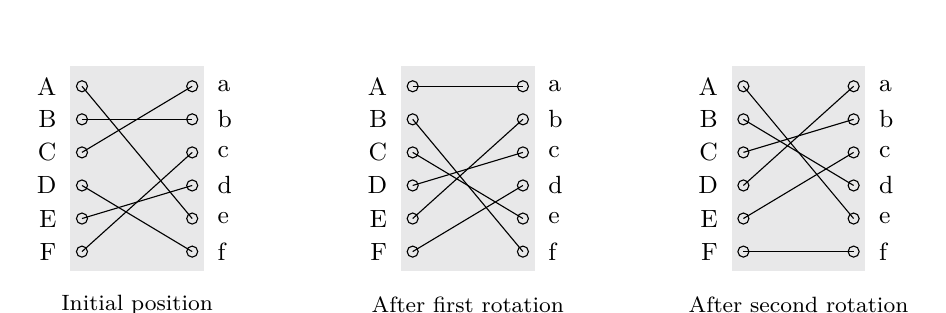
\begin{tikzpicture}[x=1cm,y=-0.42cm,font=\small]
\foreach \panel/\dx/\wires/\name in {0/0/{0/4,1/1,2/0,3/5,4/3,5/2}/Initial position, 1/4.2/{0/0,1/5,2/4,3/2,4/1,5/3}/After first rotation, 2/8.4/{0/4,1/3,2/1,3/0,4/2,5/5}/After second rotation}{
  \fill[gray!20] (\dx+0.25,-0.6) rectangle (\dx+1.95,5.6);
  \foreach \L [count=\i from 0] in {A,B,C,D,E,F}{\node[anchor=east] at (\dx+0.2,\i) {\L}; \draw (\dx+0.4,\i) circle (2pt);}
  \foreach \L [count=\i from 0] in {a,b,c,d,e,f}{\node[anchor=west] at (\dx+2.0,\i) {\L}; \draw (\dx+1.8,\i) circle (2pt);}
  \foreach \l/\r in \wires {\draw (\dx+0.4,\l) -- (\dx+1.8,\r);}
  \node[font=\footnotesize] at (\dx+1.1,6.6) {\name};
}
\end{tikzpicture}
\end{center}
\textbf{Example} (the slide's 6-letter rotor; plaintext on the right, ciphertext on the left). In the initial position \ttx{b} is wired to \ttx{B} and \ttx{e} to \ttx{A}; after the first rotation \ttx{e} is wired to \ttx{C}; after the second, \ttx{e} is wired to \ttx{A} again. If the rotor were stationary (a monoalphabetic substitution), ``bee'' would be encrypted as \ttx{BAA}. With the rotor turning after each letter it becomes \ttx{BCA}: the two \ttx{e}'s are encrypted as different characters. A single rotor of 26 contacts repeats its sequence of permutations every 26 letters, which is still a short period.

\textbf{The Enigma machine} was invented by Arthur Scherbius in 1918 for businesses that needed to send confidential documents without codebooks; it was modified by the German army and used extensively in World War II. It is based on the principle of rotor ciphers, with three rotors connected so that the \textbf{wiring changes as you type}. Its main parts are:
\begin{itemize}[leftmargin=1.4em]
  \item a \textbf{keyboard} for typing the plaintext and a \textbf{lampboard} on which the ciphertext letter lights up;
  \item a \textbf{plugboard} that swaps chosen pairs of letters on the way in and again on the way out;
  \item three \textbf{rotors}: the \emph{fast} rotor turns one position with every key press, the \emph{middle} rotor turns once per revolution of the fast rotor, and the \emph{slow} rotor once per revolution of the middle one (like the wheels of an odometer), so the sequence of substitutions repeats only after about $26^3 = 17\,576$ letters;
  \item a \textbf{reflector}, which sends the current back through the three rotors by a different path.
\end{itemize}
\begin{center}
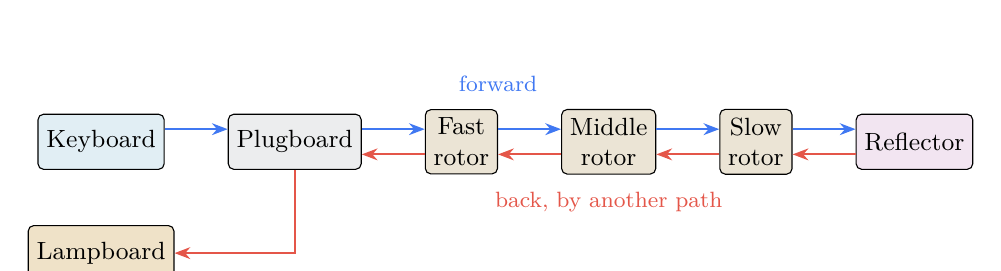
\begin{tikzpicture}[node distance=8mm]
  \node[box,fill=cyan!10] (kb) {Keyboard};
  \node[box,fill=gray!15,right=of kb] (pb) {Plugboard};
  \node[box,fill=orange!15,right=of pb] (f) {Fast\\rotor};
  \node[box,fill=orange!15,right=of f] (m) {Middle\\rotor};
  \node[box,fill=orange!15,right=of m] (s) {Slow\\rotor};
  \node[box,fill=magenta!10,right=of s] (r) {Reflector};
  \node[box,fill=yellow!20,below=7mm of kb] (lb) {Lampboard};
  \foreach \a/\b in {kb/pb,pb/f,f/m,m/s,s/r}{\draw[arr,acc] ([yshift=1.6mm]\a.east) -- ([yshift=1.6mm]\b.west);}
  \foreach \a/\b in {r/s,s/m,m/f,f/pb}{\draw[arr,warn] ([yshift=-1.6mm]\a.west) -- ([yshift=-1.6mm]\b.east);}
  \draw[arr,warn] (pb.south) |- (lb.east);
  \node[font=\footnotesize,acc,above=1mm of f.north east] {forward};
  \node[font=\footnotesize,warn,below=1mm of m.south] {back, by another path};
\end{tikzpicture}
\end{center}
In the slide's example the key \ttx{T} is pressed: the plugboard turns it into \ttx{K}, the three wheels carry it to the reflector, which returns it on another contact, the wheels carry it back to \ttx{W}, and the plugboard turns \ttx{W} into \ttx{G}, so lamp \ttx{G} lights.

\textbf{Consequences of the reflector.} The current path is reversible, so with the same settings pressing \ttx{G} lights \ttx{T}: encryption and decryption are the same operation, which made the machine convenient. But the reflector never connects a contact to itself, so the return path always ends on a different letter: \textbf{Enigma never encrypts a letter to itself}. This was a real weakness. Allied cryptanalysts used it to place a guessed plaintext word (a \emph{crib}) against the ciphertext, rejecting every position where some letter would have mapped to itself, and then searched the rotor settings with machines (the \emph{bombes}). The key of a day was the choice and order of the rotors, their ring settings and starting positions, and the plugboard pairs.

\subsection{Transposition: keyless, keyed, combined \hot}
\asked{Mid-sem 2024--25 Q3(b): ``abcdefghij'' $\to$ ``CABDEHFGIJ'' with a keyed transposition: the pattern repeats every 5 letters, so the permutation key has size \textbf{5}.}
A transposition cipher does not substitute one symbol for another; it changes the location of the symbols (\S\ref{sec:transp}). Forouzan sorts transposition ciphers by how the permutation is produced.

\textbf{Keyless transposition.} Simple transposition ciphers used in the past are keyless: the permutation comes from the shape of a table, not from a key. There are two methods. In the first, the text is written into a table \emph{column by column} and transmitted \emph{row by row}; the rail fence is this method with a 2-row table. To send ``meet me at the park'', Alice writes the letters in a zig-zag over two lines and sends the first line followed by the second: \textbf{\ttx{MEMATEAKETETHPR}}. Bob divides the ciphertext in half (here the second half, \ttx{ETETHPR}, has one character fewer than the first, \ttx{MEMATEAK}), uses the halves as the two rows and reads in zig-zag. In the second method, the text is written \emph{row by row} and transmitted \emph{column by column}. With an agreed 4 columns Alice writes \ttx{meet|meat|thep|ark} and sends \textbf{\ttx{MMTAEEHREAEKTTP}}; Bob writes the ciphertext column by column and reads it row by row.

The permutation of the second method has a visible pattern. Writing each plaintext position under the ciphertext position it moves to,
\begin{center}\small\setlength{\tabcolsep}{3.5pt}
\begin{tabular}{@{}l*{15}{c}@{}}
\toprule
Plaintext position & 01&02&03&04&05&06&07&08&09&10&11&12&13&14&15\\
Ciphertext position & 01&05&09&13&02&06&10&14&03&07&11&15&04&08&12\\
\bottomrule
\end{tabular}
\end{center}
the second character has moved to the fifth position, the third to the ninth, and so on. The permutation falls into runs $(01, 05, 09, 13)$, $(02, 06, 10, 14)$, $(03, 07, 11, 15)$, $(04, 08, 12)$, in each of which adjacent numbers differ by 4, the number of rows. Such regularity is what the pattern attack below exploits.

\textbf{Keyed (block) transposition.} Instead of permuting the whole text at once, the plaintext is divided into groups of a predetermined size, called \textbf{blocks}, and the characters of each block are permuted separately with a \textbf{permutation key}. Alice and Bob agree to send ``Enemy attacks tonight'' in blocks of five, adding a bogus character \ttx{z} to fill the last block: \ttx{enemy attac kston ightz}. With the encryption key \textbf{(3 1 4 5 2)}, \emph{position $i$ of the ciphertext block takes the character at position key[$i$] of the plaintext block}: the third character becomes the first, the first becomes the second, the fourth the third, and so on. So \ttx{enemy} $\to$ \ttx{EEMYN}, and the ciphertext is \textbf{\ttx{EEMYN TAACT TKONS HITZG}}. Bob divides the ciphertext into 5-character groups and applies the key in the reverse direction. Since letters are only moved, changing one plaintext letter changes exactly one ciphertext letter.

\textbf{The past-paper question.} Eve types ``abcdefghij'' on Alice's computer and sees ``CABDEHFGIJ''. This is a \textbf{chosen-plaintext attack}, and the choice of plaintext is clever: all letters are different, so each output letter reveals its source position directly. \ttx{abcde} $\to$ \ttx{CABDE} and \ttx{fghij} $\to$ \ttx{HFGIJ} both take input positions 3, 1, 2, 4, 5, so the pattern repeats every 5 letters: the key has size \textbf{5}, the encryption key is \textbf{(3 1 2 4 5)}, and the decryption key is its inverse \textbf{(2 3 1 4 5)}.

\textbf{Combining the two approaches (keyed columnar transposition).} More recent transposition ciphers combine the two approaches to achieve better scrambling. Encryption is done in three steps: the text is \textbf{written into a table row by row}, the \textbf{columns are permuted} with the key, and the new table is \textbf{read column by column}. The first and third steps give a keyless \emph{global} reordering, and the second a \emph{blockwise keyed} reordering (each row is a block). Such ciphers are called \textbf{keyed columnar} or simply \textbf{columnar transposition ciphers}. With the key (3 1 4 5 2):
\begin{center}\small
\begin{tabular}{@{}c@{\quad}c@{\quad}c@{}}
Written row by row & Columns permuted (3 1 4 5 2) & Read column by column\\[2pt]
\begin{tabular}{|ccccc|}\hline e&n&e&m&y\\ a&t&t&a&c\\ k&s&t&o&n\\ i&g&h&t&z\\\hline\end{tabular}
&
\begin{tabular}{|ccccc|}\hline E&E&M&Y&N\\ T&A&A&C&T\\ T&K&O&N&S\\ H&I&T&Z&G\\\hline\end{tabular}
&
\ttx{ETTH EAKI MAOT YCNZ NTSG}
\end{tabular}
\end{center}
Ciphertext \textbf{\ttx{ETTHEAKIMAOTYCNZNTSG}}. Bob reverses the steps: he writes the ciphertext column by column, permutes the columns with the decryption key, and reads row by row.

\begin{trap}[: two ways to write a column key]
The Neso row--column key (\S\ref{sec:transp}) writes above each column its \emph{rank in the reading order} (4 3 1 2 5 6 7 means column 3 is read first). Forouzan's key lists, for each output position, the \emph{source column} (3 1 4 5 2 means column 3 goes first). The two notations are inverse permutations of each other: the Neso key 4 3 1 2 5 6 7 is Forouzan's (3 4 2 1 5 6 7). State which convention you use.
\end{trap}

\subsection{Encryption and decryption keys of a transposition}
A single key is used in two directions for the column exchange: downward for encryption and upward for decryption. It is customary to create two keys from it, one for encryption and one for decryption, each stored as a table with one entry per column. \textbf{Each entry shows the source column number; the destination column number is understood from the position of the entry.} The encryption key (3 1 4 5 2) says that column 3 of the source becomes column 1 of the destination; the decryption key (2 5 1 3 4) says that column 2 of the source becomes column 1 of the destination.

\textbf{Inverting a key.} Encryption sends source column $e_i$ to destination $i$. Decryption must send it back: the column now at position $i$ must return to position $e_i$, i.e.\ the decryption key has the entry $i$ at position $e_i$. Hence the algorithm on the slide:
\begin{center}\small\ttfamily
\begin{tabular}{@{}l@{}}
for index = 1 to Column:\quad DecKey[EncKey[index]] $\leftarrow$ index
\end{tabular}
\end{center}
By hand: write the index $1, 2, \dots$ under the encryption key, swap the two rows, and sort the pairs by the (former) key row; the index row becomes the decryption key. For the slide's key (2 6 3 1 4 7 5):
\begin{center}\small
\begin{tabular}{@{}l*{7}{c}@{\qquad}l*{7}{c}@{}}
\toprule
Encryption key & 2&6&3&1&4&7&5 & Sorted by key & 1&2&3&4&5&6&7\\
Index & 1&2&3&4&5&6&7 & Index $=$ decryption key & \textbf{4}&\textbf{1}&\textbf{3}&\textbf{5}&\textbf{7}&\textbf{2}&\textbf{6}\\
\bottomrule
\end{tabular}
\end{center}
Check: key value 1 stood at index 4, so DecKey[1] $= 4$; key value 2 stood at index 1, so DecKey[2] $= 1$. Likewise (3 1 4 5 2) inverts to (2 5 1 3 4).

\textbf{Transposition as a matrix.} The plaintext and ciphertext blocks can be written as $1 \times m$ row vectors of letter values and the key as an $m \times m$ \textbf{permutation matrix}, in which every row and every column has exactly one 1 and the rest are 0s. Column $j$ of the key has its 1 in row key[$j$], so multiplying a block by it copies input position key[$j$] to output position $j$. Encryption is $C = PK$ and decryption $P = CK^{-1}$, as in the Hill cipher; a transposition is a Hill cipher whose matrix only moves letters. The inverse needs no computation: $K^{-1} = K^{T}$. Indeed $(KK^T)_{ij} = \sum_l K_{il}K_{jl}$; for $i = j$ the single 1 of row $i$ meets itself and the sum is 1, while for $i \ne j$ the 1s of rows $i$ and $j$ lie in different columns (each column has only one 1) and the sum is 0. With the key (3 1 4 5 2) and the four blocks of ``enemyattackstonightz'' as rows:
\[
\small
\begin{pmatrix}04&13&04&12&24\\00&19&19&00&02\\10&18&19&14&13\\08&06&07&19&25\end{pmatrix}
\begin{pmatrix}0&1&0&0&0\\0&0&0&0&1\\1&0&0&0&0\\0&0&1&0&0\\0&0&0&1&0\end{pmatrix}
=
\begin{pmatrix}04&04&12&24&13\\19&00&00&02&19\\19&10&14&13&18\\07&08&19&25&06\end{pmatrix}
\]
that is \ttx{EEMYN TAACT TKONS HITZG}, the keyed block transposition above; multiplying by $K^T$ returns \ttx{enemy attac kston ightz}.

\subsection{Cryptanalysis of transposition ciphers}
Transposition ciphers are vulnerable to several kinds of ciphertext-only attack.

\textbf{Statistical attack.} Single-letter frequency analysis does not reveal the key, but since the letters are unchanged it immediately shows that the cipher is a transposition (and what language the plaintext is in); digram and trigram statistics then guide the reordering.

\textbf{Brute-force attack.} Eve can try all possible keys, but if the key length is unknown their number is huge, $1! + 2! + 3! + \dots + L!$ for an $L$-letter ciphertext. A better approach is to guess the number of columns. If the table is full, the number of columns divides $L$: for $L = 20 = 2 \times 2 \times 5$ it is one of $1, 2, 4, 5, 10, 20$, where 1 column (no change) is out of the question and 20 (a single row) is unlikely. For each candidate $c$ only $c!$ orders remain ($5! = 120$ for $c = 5$).

\textbf{Pattern attack.} The ciphertext of a keyed (columnar) transposition has repeated patterns. For the ciphertext \ttx{ETTHEAKIMAOTYCNZNTSG} above, the plaintext positions of the ciphertext letters are
\begin{center}\small\ttfamily
03 08 13 18 \;01 06 11 16 \;04 09 14 19 \;05 10 15 20 \;02 07 12 17
\end{center}
The first ciphertext character comes from the third plaintext character, and within each group of four adjacent numbers differ by 5, the number of columns. If Eve knows or guesses that there are 5 columns, she organises the ciphertext in groups of four characters (each group is one column of the table), and permuting the groups ($5! = 120$ orders at most, far fewer with digram clues) reveals the plaintext.

\textbf{Double transposition.} Double transposition ciphers make the cryptanalyst's job much harder. The whole algorithm is applied twice, normally with the same key (a different key can be used in each step). Encrypting the middle text \ttx{ETTHEAKIMAOTYCNZNTSG} again with (3 1 4 5 2) gives the ciphertext \textbf{\ttx{TIYTEAOZHMCSEANGTKTN}}, whose plaintext positions are
\begin{center}\small\ttfamily
13 16 05 07 03 06 14 20 18 04 10 12 01 09 15 17 08 11 19 02
\end{center}
No constant difference survives, so grouping the ciphertext by columns no longer gives pieces of plaintext rows. The single-letter frequency attack still works (the letters are still those of the plaintext), but the pattern attack is now much more difficult. As in \S\ref{sec:transp}, the double transposition is still one permutation of the 20 positions; what it removes is the regular columnar structure that the pattern attack depends on.

\subsection{Stream vs.\ block ciphers}
Symmetric ciphers fall into two broad categories. In a \textbf{stream cipher}, encryption and decryption are done \textbf{one symbol (a character or a bit) at a time}. There is a plaintext stream $P = P_1P_2P_3\dots$, a ciphertext stream $C = C_1C_2C_3\dots$ and a key stream $K = (k_1, k_2, k_3, \dots)$, and
\[
C_1 = E_{k_1}(P_1),\quad C_2 = E_{k_2}(P_2),\quad C_3 = E_{k_3}(P_3),\ \dots
\]
The ciphers differ only in how the key stream is made: the additive cipher repeats one value ($k_i = k$), the monoalphabetic cipher uses one fixed table, Vigen\`ere repeats $m$ values, the autokey takes its values from the plaintext, the rotor cipher uses the sequence of rotor positions, and the one-time pad uses fresh random values.

In a \textbf{block cipher}, a group of plaintext symbols of size $m$ ($m > 1$) is encrypted \textbf{together}, creating a ciphertext group of the same size. A single key is used to encrypt the whole block, even if the key is made of several values, and \textbf{each ciphertext block depends on the whole plaintext block}. Playfair ($m = 2$: the output for a letter depends on its partner) and Hill ($m \times m$ key) are block ciphers, and so are the modern DES and AES (64- and 128-bit blocks, \S\ref{sec:modern}). In practice the two ideas are combined: a block cipher encrypts the blocks of a long message one after another, so at the level of single blocks it is a block cipher, but considering each block as one unit the message is processed as a stream of blocks.

The difference shows in how far one plaintext change spreads, which past papers ask directly:
\begin{center}\small
\begin{tabular}{@{}lcl@{}}
\toprule
Cipher & Ciphertext characters changed & Reason\\
\midrule
Additive, multiplicative, affine & 1 & monoalphabetic, letter by letter\\
Vigen\`ere, one-time pad & 1 & stream: one key value per letter\\
Autokey & 2 & $P_i$ is also the key of a later letter\\
Keyed transposition & 1 & the letter is moved, not changed\\
Playfair & 2 (usually) & the digram is one block\\
Hill with $m \times m$ key & up to $m$ & every output letter uses the whole block\\
\bottomrule
\end{tabular}
\end{center}

\begin{trap}[: Vigen\`ere is a stream cipher]
Even though the key repeats every $m$ letters, Vigen\`ere encrypts one character at a time, each with its own key element: a \textbf{stream} cipher. Playfair works on pairs, Hill on $m$-letter blocks: \textbf{block} ciphers.
\end{trap}

\section{Classical Ciphers at a Glance}
The table collects every classical cipher of the course with its key and the weakness that breaks it. The pattern is consistent: a cipher is broken through whatever structure the key fails to destroy, whether that is a tiny key space, preserved letter or digram frequencies, a period, linearity or a regular position pattern.
\begin{center}\small
\begin{tabularx}{\textwidth}{@{}l l l X@{}}
\toprule
Cipher & Type & Key & Main weakness\\
\midrule
Caesar & substitution, 1 letter & shift 3 (fixed) & algorithm known, no real key\\
Shift & substitution, 1 letter & shift 1--25 & only 25 keys: brute force\\
Multiplicative & substitution, 1 letter & $k \in \mathbb{Z}_{26}^*$ (12) & brute force; frequencies preserved\\
Affine & substitution, 1 letter & $(k_1, k_2)$: 312 keys & two known pairs give the key\\
Monoalphabetic & substitution, 1 letter & permutation ($26!$) & letter frequencies preserved\\
Playfair & substitution, 2 letters & 5$\times$5 keyword matrix & same pair $\to$ same output\\
Hill & substitution, $m$ letters & invertible $m\times m$ matrix & linear (known plaintext)\\
Vigen\`ere & polyalphabetic & repeating keyword & key repeats: Kasiski/IC, then Caesars\\
Autokey & polyalphabetic & keyword + plaintext & key has English frequencies\\
Vernam & polyalphabetic, bits (XOR) & key stream & tape key repeated\\
Rotor, Enigma & polyalphabetic, stream & wiring, rotor positions & finite period; Enigma never maps a letter to itself\\
One-time pad & substitution & random, once, message length & none (perfect secrecy); key generation and distribution\\
Rail fence & transposition & depth & few possibilities\\
Row--column & transposition & column order (+ stages) & one stage can be reconstructed\\
Keyed / columnar & transposition & permutation of $m$ positions & pattern attack (double transposition resists it)\\
\bottomrule
\end{tabularx}
\end{center}
Transposition ciphers keep the letter frequencies of the plaintext unchanged (only positions move); substitution ciphers keep the positions and change the letters.

\begin{fixbox}
\begin{itemize}[leftmargin=1.2em,itemsep=0pt]
  \item Kasiski slide: ``the cryptanalyst assumes that $d \mid m$'' and ``$\gcd(d_1, \dots, d_n)/m$'' should read $m \mid d$ and $m \mid \gcd(d_1, \dots, d_n)$: the key length divides the distances, not the other way round.
  \item Kasiski example: the indices 68/168, 69/117, 72/132, 119/127 count from 0 (from 1 they are 69/169, 70/118, 73/133, 120/128); the differences 100, 48, 60, 8 are unaffected.
  \item Kasiski example: the slide's rows P1--P4 are not the decryptions of C1--C4 from the 21st letter of each piece onward. The ciphertext was made from a copy of the sentence with typos (decrypted with key \ttx{code}, ``shift'' lacks its \ttx{f}, ``shifted'' ends in \ttx{r}, the \ttx{t} of ``to'' is missing and an extra \ttx{a} precedes ``ciphertext''), while P1--P4 were written from the corrected sentence. The key \ttx{code} and the method are right.
  \item Affine attack: ``The square matrix and its inverse are the same'' means they are the same as in the first attempt (both use the plaintext ``et''); $\left(\begin{smallmatrix}4&1\\19&1\end{smallmatrix}\right)$ is not its own inverse, which is $\left(\begin{smallmatrix}19&7\\3&24\end{smallmatrix}\right)$.
  \item Keyless transposition slide: the mapping row shows 13 under plaintext position 8 and the run $(02, 06, 10, 13)$; both should be 14. The runs are $(01,05,09,13)$, $(02,06,10,14)$, $(03,07,11,15)$, $(04,08,12)$.
  \item Double transposition slide: the ciphertext is \ttx{TIYTEAOZHMCSEANG}\textbf{\ttx{T}}\ttx{KTN}, not \ttx{\dots EANGYKTN}; in the position list the seventh entry is \textbf{14}, not a second 10.
  \item ``Keys'' slide: ``one for encryption and one for direction'' should be ``one for decryption''. Enigma slide: the inventor is Arthur \emph{Scherbius}.
  \item Stream/block slide lists ``Polyalphabetic cipher'' under block ciphers while listing Vigen\`ere under stream ciphers. By the slide's own definitions, polyalphabetic ciphers that encrypt one letter at a time (Vigen\`ere, autokey, rotor) are stream ciphers.
\end{itemize}
\end{fixbox}

% Sources: Neso videos (steganography, LSB steganography demo, abstract algebra & number theory intro, prime numbers;
% notes6.md), Stallings 2.5 (steganography). Numbers checked by script (scratchpad/r3/verify3.py).
\definecolor{puregreen}{RGB}{0,255,0}
\definecolor{modgreen}{RGB}{0,252,0}

\section{Steganography}\label{sec:stego}
Encryption hides the \emph{meaning} of a message but not the fact that a secret message is being sent. Ciphertext looks like random gibberish, so it draws attention: an observer immediately knows that something is worth intercepting, may block it, or may pressure the sender and receiver for the key. \textbf{Steganography} (Greek ``covered writing'') solves a different problem. It \textbf{conceals the existence of the message} by hiding it inside an innocent-looking \textbf{cover} such as a text, an image or an audio file, so that an observer does not suspect that any secret communication is taking place. It is \textbf{not an encryption scheme}: the message is not transformed into something unintelligible but merely hidden, and its protection lies in going unnoticed. \textbf{Cryptography}, by contrast, renders the message unintelligible to outsiders by various transformations of the text.

\imp{Cryptography hides the meaning of a message; steganography hides its existence.}
\begin{center}\small
\begin{tabularx}{\textwidth}{@{}l X X@{}}
\toprule
 & \textbf{Cryptography} & \textbf{Steganography}\\
\midrule
Hides & the \textbf{meaning} & the \textbf{existence}\\
Attacker sees & a scrambled message; knows something secret is being sent & an ordinary-looking text/image; doesn't suspect anything\\
Output & ciphertext & a normal-looking \textbf{cover} (text, image, audio) with the message inside\\
\bottomrule
\end{tabularx}
\end{center}
Steganography is the other kind of ``security-related transformation'' $T$ in the model for network security (\S\ref{sec:netmodel}): the transformation applied to the message before transmission does not have to be encryption.

\textbf{Examples from the lecture.} The simplest text steganography arranges words so that some of their letters spell the real message, here the first letter of each word (an \emph{acrostic}, or null cipher). The cover sentence reads as ordinary if odd text, and the secret is the rule ``read the first letters'':
\begin{itemize}
  \item \textbf{S}imply \textbf{e}ncrypt \textbf{c}orrect \textbf{r}eading \textbf{e}xactly \textbf{t}wice. $\Rightarrow$ \textbf{Secret}
  \item \textbf{T}ell \textbf{h}enry \textbf{a}lice \textbf{n}ot \textbf{k}ane / \textbf{Y}esterday \textbf{o}urplan \textbf{u}ndone! $\Rightarrow$ \textbf{Thank You}
\end{itemize}

\subsection{Historical techniques}
Before computers, messages were hidden physically in ordinary documents. Stallings lists four classical techniques; each leaves the document readable as normal text and reveals the hidden marks only under a special treatment that an inspector would not think of applying.
\begin{center}\small
\begin{tabularx}{\textwidth}{@{}l X@{}}
\toprule
Character marking & Chosen letters of a printed or typewritten text are overwritten faintly in pencil. The marks are not visible unless the paper is held at an angle to bright light.\\
Invisible ink & Written with a substance (e.g.\ lemon juice) that leaves no visible trace until heat or a chemical is applied.\\
Pin punctures & Tiny pin holes on selected letters. They are not visible unless the paper is held up in front of a light.\\
Typewriter correction ribbon & Text typed between the lines with a correction ribbon. It is visible only under a strong light.\\
\bottomrule
\end{tabularx}
\end{center}
Modern steganography hides data in digital media instead. Stallings' example is a high-resolution photograph (Kodak Photo CD, $2048 \times 3072$ pixels of 24 bits): changing only the least significant bit of each colour byte does not visibly affect the picture, yet hides $2048 \times 3072 \times 3 = 18\,874\,368$ bits, about 2.3 MB, in a single snapshot. This LSB method is explained below.

\subsection{Drawbacks}
Compared with encryption, steganography has two drawbacks.
\begin{enumerate}[leftmargin=1.5em]
  \item \textbf{Lots of overhead.} A large cover is needed to hide relatively few bits of message: a whole sentence for six letters in the acrostic above, a whole image for a few kilobytes.
  \item \textbf{Once the system is discovered, it becomes virtually worthless.} The security rests entirely on the method staying unknown, which contradicts Kerckhoff's principle (\S\ref{sec:attacks}). Unlike encryption, there is no secret key left to protect the message once the method is known. This can be softened by making the insertion depend on a key (for example, a key that selects which pixels carry the bits).
\end{enumerate}
\textbf{Advantage.} Steganography can be used by parties who have something to lose if the \emph{fact} of their secret communication (not necessarily its content) is discovered. Encryption flags the traffic as important or secret, and may mark the sender or receiver as someone with something to hide; a stego image is just a photograph.

\textbf{Best of both.} A message can be \textbf{first encrypted and then hidden} using steganography. The hiding conceals that communication is taking place, and if the hiding is discovered the attacker still only has ciphertext, which is protected by the key. Encrypted data also looks random, like the noise in the least significant bits it replaces, which makes the hidden data harder to detect statistically.
\begin{center}
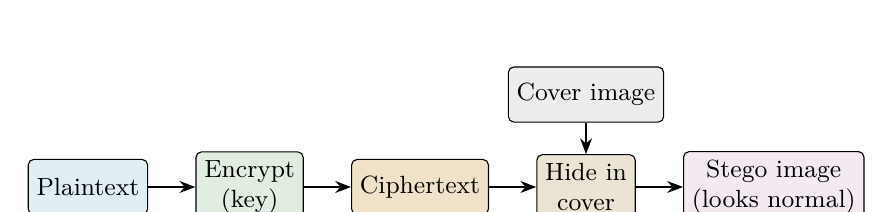
\begin{tikzpicture}[node distance=6mm]
  \node[box,fill=cyan!10] (p) {Plaintext};
  \node[box,fill=green!15,right=of p] (e) {Encrypt\\(key)};
  \node[box,fill=yellow!20,right=of e] (c) {Ciphertext};
  \node[box,fill=orange!15,right=of c] (h) {Hide in\\cover};
  \node[box,fill=gray!15,above=4mm of h] (cv) {Cover image};
  \node[box,fill=magenta!8,right=of h] (s) {Stego image\\(looks normal)};
  \draw[arr] (p)--(e); \draw[arr] (e)--(c); \draw[arr] (c)--(h); \draw[arr] (cv)--(h); \draw[arr] (h)--(s);
\end{tikzpicture}
\end{center}

\subsection{LSB steganography}
A byte $b_7 b_6 \dots b_1 b_0$ has the value $128 b_7 + 64 b_6 + \dots + 2 b_1 + b_0$. The leftmost bits are the \textbf{most significant bits} (MSB), because changing them changes the value a lot; the rightmost bits are the \textbf{least significant bits} (LSB), which change it the least:
\[
1010\,10\underbrace{01}_{\text{LSBs}} \qquad\text{bit weights: } 128\;64\;32\;16\;8\;4\;\underline{2\;1}
\]
Changing the lowest $k$ bits of a byte changes its value by at most $2^k - 1$. For $k = 2$ that is at most 3 out of 255, about 1.2\% of the range, which the eye cannot see in a colour.

\textbf{RGB model.} In a 24-bit colour image each pixel is stored as three bytes, one each for the intensity of \textbf{Red}, \textbf{Green} and \textbf{Blue} (0--255).
\begin{center}\small Red $(255,0,0) = (\ttx{11111111}, \ttx{00000000}, \ttx{00000000})$ \quad Green $(0,255,0)$ \quad Blue $(0,0,255)$\end{center}

\begin{center}
\begin{tikzpicture}
  \fill[puregreen] (0,0) rectangle (3.2,1.4);
  \fill[modgreen] (4.2,0) rectangle (7.4,1.4);
  \node[font=\small,below] at (1.6,0) {$(0, 255, 0)$, G $=$ \ttx{111111\textbf{11}}};
  \node[font=\small,below] at (5.8,0) {$(0, 252, 0)$, G $=$ \ttx{111111\textbf{00}}};
\end{tikzpicture}
\end{center}
The two boxes look identical, but the last 2 bits of their green values differ. \textbf{Those LSBs can therefore store hidden information}: the sender overwrites them with message bits, and the image looks unchanged. Using the 2 LSBs of each of R, G and B hides $2 \times 3 = \mathbf{6}$ \textbf{bits per pixel}, and no channel value changes by more than 3. To extract the message the receiver simply reads the last 2 bits of each channel, in the agreed order of pixels, and concatenates them.

\begin{worked}[: hiding bits in one pixel]
\textbf{Q.} Hide the six bits \ttx{11 01 10} in the pixel $(100, 50, 200)$ using the 2 LSBs of each channel. By how much does each value change?

Write each value in binary and replace its last two bits with the next two message bits:
\begin{center}\small
\begin{tabular}{@{}lllll@{}}
\toprule
Channel & Value & Binary & Replace last 2 bits & New value\\
\midrule
R & 100 & \ttx{011001\textbf{00}} & \ttx{011001\textbf{11}} & 103 ($+3$)\\
G & 50 & \ttx{001100\textbf{10}} & \ttx{001100\textbf{01}} & 49 ($-1$)\\
B & 200 & \ttx{110010\textbf{00}} & \ttx{110010\textbf{10}} & 202 ($+2$)\\
\bottomrule
\end{tabular}
\end{center}
New pixel \textbf{(103, 49, 202)}; every channel changes by at most 3, as predicted. Check: the last two bits of 103, 49, 202 are \ttx{11}, \ttx{01}, \ttx{10} \checkmark.
\end{worked}

\textbf{Capacity.} With 6 bits per pixel an $800 \times 600$ image holds $800 \cdot 600 \cdot 6 = 2{,}880{,}000$ bits $= 360{,}000$ bytes. With only the single LSB of each channel (3 bits per pixel) a $1024 \times 768$ image holds $1024 \cdot 768 \cdot 3 = 2{,}359{,}296$ bits $= 294{,}912$ bytes. The lecture's 17-byte message ``Kill Corona Virus'' is $17 \times 8 = 136$ bits, which needs only $\lceil 136 / 6 \rceil = 23$ pixels at 6 bits per pixel.

\textbf{Blue orchids:} the lecture shows the image without and with hidden information side by side, and they cannot be told apart.

\textbf{Detection.} Looking at the image reveals nothing, but a statistical analysis may. In a natural photograph the LSBs are correlated with the rest of the image, while embedded data (especially encrypted data) is uniformly random, so the LSB plane of a stego image has slightly different statistics; a changed file format or file size is a further clue (see the OpenStego demo below). The study of detecting hidden data is called \textbf{steganalysis}.

\subsection{Watermarking vs.\ image steganography}
Both techniques embed extra information in an image, but for opposite purposes. A \textbf{watermark} is embedded to \textbf{prove ownership} or copyright: the logo or owner information is not secret, it is often visible (like the \ttx{nesoacademy.org} mark on the lecture's laptop image), and it must survive cropping and compression so that it can still be shown later. \textbf{Image steganography} embeds a message for \textbf{secret communication}: its \textbf{existence} must stay hidden, and robustness matters less than going unnoticed.
\begin{center}\small
\begin{tabularx}{\textwidth}{@{}l X X@{}}
\toprule
 & \textbf{Watermarking} & \textbf{Image steganography}\\
\midrule
Purpose & prove \textbf{ownership} / copyright & \textbf{secret communication}\\
Is the mark secret? & no; it's often visible (like the \ttx{nesoacademy.org} logo) & yes; its \textbf{existence} is hidden\\
Hidden data & logo, owner info & any message or file\\
\bottomrule
\end{tabularx}
\end{center}

\subsection{OpenStego demo}
OpenStego is a free tool that embeds a file in an image and extracts it again. The lecture uses it in both directions:
\begin{enumerate}[leftmargin=1.5em]
  \item \textbf{Hide Data:} message file \ttx{My Message.txt} (``Kill Corona Virus'', 17 bytes) + cover file \ttx{Blue Orchids.jpg} (58.4 KB) $\to$ stego file \ttx{BO.png} (824 KB). No password. ``Message embedded into 1 cover file(s).''
  \item \textbf{Extract Data:} input \ttx{BO.png} $\to$ output folder. ``Message file extracted successfully'', and the text file comes back unchanged.
\end{enumerate}
\textbf{Why PNG, and why so much bigger} (not explained in the video): JPEG compression is lossy, so it slightly changes pixel values when the image is saved, which would wipe out the hidden LSBs. The stego image is therefore saved in the lossless PNG format, which stores every pixel exactly and is much larger (58.4 KB $\to$ 824 KB). That size jump is itself a hint that something is going on. Leaving the password empty means the extraction needs no key, so anyone who suspects the file and has the tool can read the message; with a password OpenStego encrypts the data before hiding it, which is the encrypt-then-hide combination above.

\section{Prime Numbers}\label{sec:primesintro}
\textbf{Why the course turns to mathematics.} Classical ciphers substitute and move letters. Modern cryptography treats plaintext and ciphertext as \emph{numbers}, and most encryption is based heavily on \textbf{number theory} and \textbf{abstract algebra}; calculus and trigonometry make no major contribution. The concepts needed are the division and Euclidean algorithms and the extended Euclidean algorithm (\S\ref{sec:exteuclid}), modular arithmetic (\S\ref{sec:modular}), groups, rings, fields and finite fields with polynomial arithmetic (\S\ref{sec:algebra}), Euler's totient (\S\ref{sec:totient}), Fermat's and Euler's theorems (\S\ref{sec:fermat}), and primality testing, the Chinese remainder theorem and discrete logarithms (\S\ref{sec:primes}). The lecture also notes that this is cryptography for classical computers; quantum computers will need different assumptions, because a quantum algorithm (Shor's) factors efficiently. Primes come first because almost everything else is built on them.

\textbf{Definitions.} A \textbf{prime} is an integer greater than 1 with exactly two divisors, 1 and itself: it cannot be divided by any other number without leaving a remainder. A \textbf{composite} number has more than two divisors. \textbf{1 is neither}, because it has only one divisor. Examples: 2, 3, 5, 7 are prime; $9 = 3^2$ (divisors 1, 3, 9) and $33 = 3 \cdot 11$ (divisors 1, 3, 11, 33) are composite.

\textbf{Facts.} 2 is the smallest prime and the \textbf{only even prime}, since every larger even number has 2 as a third divisor. Except for 2 and 5, every prime ends in the digit 1, 3, 7 or 9: a number ending in 0, 2, 4, 6 or 8 is divisible by 2, and one ending in 5 is divisible by 5. (The converse fails: $33$ and $39$ end in 3 and 9 but are composite.)

\textbf{Every number has prime factors.} By the \textbf{fundamental theorem of arithmetic}, every integer $n > 1$ can be written as a product of primes in exactly one way, apart from the order of the factors. A prime is its own factorisation; 1 is not a factor to be listed, since it is not prime.
\begin{center}\small
\begin{tabular}{@{}rl@{\qquad}rl@{}}
\toprule
$n$ & factorisation & $n$ & factorisation\\
\midrule
10 & $2 \cdot 5$ & 37 & $37$ (prime)\\
11 & $11$ (prime) & 308 & $2^2 \cdot 7 \cdot 11$\\
100 & $2^2 \cdot 5^2$ (9 divisors) & 14688 & $2^5 \cdot 3^3 \cdot 17$\\
\bottomrule
\end{tabular}
\end{center}
The number of divisors follows from the factorisation: a divisor of $2^2 \cdot 5^2$ is $2^a 5^b$ with $a, b \in \{0, 1, 2\}$, giving $3 \times 3 = 9$ divisors of 100 (1, 2, 4, 5, 10, 20, 25, 50, 100).

\subsection{Why primes matter in cryptography}
Many encryption algorithms, RSA first among them (\S\ref{sec:rsa}), are based on prime numbers, because of an asymmetry in the work involved. \textbf{Multiplying} two large primes is \textbf{very fast}: two 300-digit numbers are multiplied in a fraction of a millisecond. The \textbf{reverse}, \textbf{factoring} the product back into its primes, is \textbf{extremely computer-intensive}: no known classical algorithm does it in polynomial time, and for a product of two well-chosen 1024-bit primes all the computers in the world would take far too long (\S\ref{sec:primes} covers the factoring methods).
\[
p, q \;\xrightarrow{\text{easy}}\; n = p \cdot q \qquad\qquad n \;\xrightarrow{\text{very hard}}\; p, q
\]
A function that is easy to compute but infeasible to reverse is called a \textbf{one-way function}; if a secret (here the primes $p$ and $q$) makes the reverse easy, it is a \textbf{trapdoor one-way function}, which is exactly what a public-key cipher needs. Cryptographic algorithms therefore use \textbf{large} primes, hundreds of digits long. The lecture closes with six numbers to test, from 4 to 34 digits: 5393, 27644437, 4398042316799, 1125899839733759, 18014398241046527 and 1298074214633706835075030044377087. \textbf{All six are prime} (checked with the Miller--Rabin test of \S\ref{sec:primes}); trial division would need about $\sqrt{n}$ steps, which is hopeless for the last one, and this is why fast probabilistic primality tests matter.

\begin{mustknow}[: primes]
Prime: $> 1$ with exactly two divisors (1 and itself); 1 is not prime; 2 is the only even prime. Every $n > 1$ factors uniquely into primes, e.g.\ $14688 = 2^5 \cdot 3^3 \cdot 17$.\\
Security of RSA-type systems rests on \textbf{factoring the product} $n = pq$ of two large primes being infeasible, while multiplying $p$ and $q$ is easy.
\end{mustknow}

\begin{fixbox}
\begin{itemize}
  \item \textbf{Slide wording:} ``Factoring very large prime numbers is very hard'' should say factoring the \emph{product} of two large primes. A prime can't be factored at all.
  \item The factorisation table writes $11 = 1^1 \times 11^1$ and lists 1 as a prime factor. 1 is not prime; 11 and 37 are simply prime.
  \item The notes call watermarks ``typically visible''. The lecture's example is visible, but watermarks can also be invisible. The real difference is the purpose (ownership vs.\ secret communication).
  \item Fermat's and Euler's theorems need $\gcd(a,p) = 1$ / $\gcd(a,n) = 1$; the notes omitted this condition.
  \item Everything else checked: TOMATO $\to$ (a) (by script), $N(N-1)/2$, all six numbers prime, factorisations correct.
\end{itemize}
\end{fixbox}

% College Lecture 2 (integer division) + Lecture 4 (modular arithmetic, inverses, Z_n, Z_n^*), Neso videos on modular
% arithmetic (notes7.md), Forouzan ch. 2 (2.1, 2.2, 2.4 linear congruences). Every number recomputed by script (scratchpad/r4/verify.py).
\section{Modular Arithmetic}\label{sec:modular}

Modular arithmetic is integer arithmetic in which only the remainder after division by a fixed positive integer $n$ is kept, so that counting wraps around to 0 after reaching $n - 1$. Cryptography needs it for two reasons. First, a cipher must map a finite alphabet onto itself: shifting Y by 3 has to land on a letter again, which is achieved by wrapping around after 25. Second, public-key systems compute with numbers that are hundreds of digits long, and modular arithmetic keeps every intermediate result below the modulus however many operations are performed. This section builds the arithmetic from the division algorithm and ends with the two questions that recur in every later chapter: when can we divide modulo $n$, and how do we solve $ax \equiv b \pmod n$.

\subsection{Integer division and residues}
The set of integers $\mathbb{Z} = \{\dots, -2, -1, 0, 1, 2, \dots\}$ is closed under the three binary operations cryptography uses (addition, subtraction and multiplication) but not under division, since $7/2$ is not an integer. Integer division therefore has two outputs instead of one. \imp{For any integer $a$ and any positive integer $n$ there are unique integers $q$ (the quotient) and $r$ (the remainder) with $a = q \times n + r$ and $0 \le r < n$.} This statement is the \textbf{division algorithm}. For $a = 255$ and $n = 11$ it gives $255 = 23 \times 11 + 2$, so $q = 23$ and $r = 2$.

The pair $(q, r)$ is unique because of the condition $0 \le r < n$: if $a = qn + r = q'n + r'$, then $r - r' = (q' - q)n$ is a multiple of $n$ lying strictly between $-n$ and $n$, so it is 0. Geometrically, $qn$ is the largest multiple of $n$ that does not exceed $a$, and $r$ is the distance from that multiple up to $a$. The picture settles the case of a negative $a$ as well: the largest multiple of $n$ not exceeding $a$ then lies to the \emph{left} of $a$, further from zero, so $r$ is still non-negative.
\begin{center}
\begin{tikzpicture}[x=10mm,y=1mm,font=\footnotesize]
  % positive a
  \draw[-{Stealth[length=2mm]}] (-0.4,0) -- (8.7,0);
  \foreach \x/\l in {0/0,1.2/11,2.4/22,6/253,8.2/264}{\draw (\x,1.5) -- (\x,-1.5) node[below]{\l};}
  \node at (4.2,-4) {$\cdots$};
  \fill[acc] (6.4,0) circle (0.6mm) node[above=0.5mm,acc]{$a = 255$};
  \draw[{Stealth[length=1.2mm]}-{Stealth[length=1.2mm]},good,thick] (6,-9) -- node[below]{$r = 2$} (6.4,-9);
  \node[anchor=west,gray] at (8.9,0) {$a \ge 0$: $255 = 23 \times 11 + 2$};
  % negative a
  \begin{scope}[yshift=-27mm]
  \draw[-{Stealth[length=2mm]}] (-0.4,0) -- (8.7,0);
  \foreach \x/\l in {0/$-264$,2.2/$-253$,5.8/$-22$,7/$-11$,8.2/0}{\draw (\x,1.5) -- (\x,-1.5) node[below]{\l};}
  \node at (4,-4) {$\cdots$};
  \fill[acc] (1.8,0) circle (0.6mm) node[above=0.5mm,acc]{$a = -255$};
  \draw[{Stealth[length=1.2mm]}-{Stealth[length=1.2mm]},good,thick] (0,-9) -- node[below]{$r = 9$} (1.8,-9);
  \draw[{Stealth[length=1.2mm]}-,warn,dashed] (1.8,-9) -- (2.2,-9) node[right,warn]{truncated: $-2$};
  \node[anchor=west,gray] at (8.9,0) {$a < 0$: $-255 = (-24) \times 11 + 9$};
  \end{scope}
\end{tikzpicture}
\end{center}

\textbf{Negative dividends.} C, Java and many calculators divide by truncating towards zero, which for a negative $a$ returns a negative quotient and a negative remainder: $-255 = (-23) \times 11 + (-2)$. Such an $r$ violates $0 \le r < n$. The fix on the slide is to decrement $q$ by 1 and add $n$ to $r$, which leaves the right-hand side unchanged because $(q - 1)n + (r + n) = qn + r$: $-255 = (-24) \times 11 + 9$, so the remainder is 9. In practice the rule is: \textbf{if the remainder comes out negative, add the modulus}. (Python's \ttx{\%} already does this: \ttx{-255 \% 11} is 9.)

\textbf{The modulo operator.} Modular arithmetic keeps only the second output of the division algorithm. \imp{$a \bmod n$ is the remainder $r$ of dividing $a$ by $n$; $n$ is called the modulus and $r$ the residue.} The residue always lies in the \textbf{set of least residues modulo $n$}, $\mathbb{Z}_n = \{0, 1, 2, \dots, n-1\}$; for example $\mathbb{Z}_2 = \{0, 1\}$, $\mathbb{Z}_6 = \{0, 1, \dots, 5\}$ and $\mathbb{Z}_{11} = \{0, 1, \dots, 10\}$. The slide examples are $27 \bmod 5 = 2$, $36 \bmod 12 = 0$, $-18 \bmod 14 = 10$ (truncated remainder $-4$, plus 14) and $-7 \bmod 10 = 3$ (truncated remainder $-7$, plus 10). A 12-hour clock is arithmetic modulo 12 that writes 12 in place of 0: 15:00 shows 3 because $15 \bmod 12 = 3$, and 23:00 shows 11.

\textbf{Divisibility.} When the remainder is zero, $a = q \times n$ and we say that $n$ \emph{divides} $a$, written $n \mid a$; otherwise $n \nmid a$. Thus $4 \mid 32$ because $32 = 8 \times 4$, while $8 \nmid 42$ because $42 = 5 \times 8 + 2$. The properties of divisibility and the greatest common divisor are developed in \S\ref{sec:gcd}.

\subsection{Congruence and residue classes}
The mod operator sends infinitely many integers to the same residue: 2, 12, 22 and $-8$ all leave remainder 2 on division by 10. In cryptography it is this common remainder that matters, not the particular integer, so we need a relation that says ``same remainder'' without reducing anything. \imp{Two integers are congruent modulo $n$, written $a \equiv b \pmod n$, if $n \mid (a - b)$.} Equivalently, $a = kn + b$ for some integer $k$, or $a \bmod n = b \bmod n$.

The last equivalence is what makes the definition useful, and it follows from the division algorithm. Write $a = q_1 n + r_1$ and $b = q_2 n + r_2$ with $0 \le r_1, r_2 < n$. Then $a - b = (q_1 - q_2)n + (r_1 - r_2)$, and since $|r_1 - r_2| < n$, the difference is a multiple of $n$ exactly when $r_1 = r_2$. As a result the fastest validity test for a congruence is to subtract and check divisibility; neither side has to be reduced.

Congruence must be read differently from both equality and the operator. $10 \equiv -2 \pmod{12}$ is true although $10 \ne -2$, and $38 \equiv 14 \pmod{12}$ is true although $38 \bmod 12 = 2$, not 14. The operator ``$\bmod$'' returns one specific number in $\mathbb{Z}_n$, while ``$\equiv \dots \pmod n$'' states that two integers lie in the same class and allows any representative on either side. The eight statements from the lecture video:
\begin{center}\small
\begin{tabular}{@{}llll@{}}
\toprule
Statement & $a - b$ & Divisible by $m$? & Verdict\\
\midrule
$38 \equiv 2 \pmod{12}$ & 36 & yes & \textbf{valid} (and $38 \bmod 12 = 2$)\\
$38 \equiv 14 \pmod{12}$ & 24 & yes & \textbf{valid} (but $38 \bmod 12 = 2$, not 14)\\
$5 \equiv 0 \pmod 5$ & 5 & yes & \textbf{valid}\\
$10 \equiv 2 \pmod 6$ & 8 & no & \textbf{invalid}\\
$13 \equiv 3 \pmod{13}$ & 10 & no & \textbf{invalid}\\
$2 \equiv -3 \pmod 5$ & 5 & yes & \textbf{valid}\\
$-8 \equiv 7 \pmod 5$ & $-15$ & yes & \textbf{valid}\\
$-3 \equiv -8 \pmod 5$ & 5 & yes & \textbf{valid}\\
\bottomrule
\end{tabular}
\end{center}

\textbf{Congruence is an equivalence relation.} It is reflexive ($a \equiv a$, since $n \mid 0$), symmetric (if $n \mid a - b$ then $n \mid b - a$) and transitive (if $n \mid a - b$ and $n \mid b - c$, then $n$ divides their sum $a - c$). Any equivalence relation splits its set into disjoint classes of mutually related elements. \imp{The residue class $[a]_n$ is the set of all integers congruent to $a$ modulo $n$}, that is, $[a]_n = \{\dots, a - 2n, a - n, a, a + n, a + 2n, \dots\}$. Modulo $n$ there are exactly $n$ classes, one for each possible remainder. For $n = 5$:
\[
\begin{aligned}
[0] &= \{\dots, -15, -10, -5, 0, 5, 10, 15, \dots\} & [1] &= \{\dots, -14, -9, -4, 1, 6, 11, 16, \dots\} & [2] &= \{\dots, -13, -8, -3, 2, 7, 12, 17, \dots\}\\
[3] &= \{\dots, -12, -7, -2, 3, 8, 13, 18, \dots\} & [4] &= \{\dots, -11, -6, -1, 4, 9, 14, 19, \dots\}
\end{aligned}
\]
$\mathbb{Z}_n$ is obtained by choosing the smallest non-negative member of each class, which is why its elements are called the \emph{least residues}. Any member of a class can stand in for any other inside a congruence, so $-8 \equiv 2 \equiv 12 \equiv 22 \pmod{10}$ all describe the single element 2 of $\mathbb{Z}_{10}$. The slides draw $\mathbb{Z}$ as a line and $\mathbb{Z}_n$ as a circle of $n$ points: moving $n$ steps along the line brings you back to the same point of the circle.

\subsection{Operations in \texorpdfstring{$\mathbb{Z}_n$}{Zn}: why reducing first is allowed}
Addition, subtraction and multiplication in $\mathbb{Z}_n$ are defined by computing in $\mathbb{Z}$ and mapping the result back with $\bmod\ n$. The slide examples: adding 7 to 14 in $\mathbb{Z}_{15}$ gives $21 \bmod 15 = 6$; subtracting 11 from 7 in $\mathbb{Z}_{13}$ gives $-4 \bmod 13 = 9$; multiplying 11 by 7 in $\mathbb{Z}_{20}$ gives $77 \bmod 20 = 17$. The difficulty is size. The product $1{,}723{,}345 \times 2{,}124{,}945$ already has 13 digits; in RSA the operands have over 300 digits, and a power such as $C^d$ computed in full would have more digits than there are atoms in the universe. We must reduce the operands \emph{before} operating, and that needs a proof that the result does not change.

\textbf{Derivation.} Write $a = q_1 n + r_1$ and $b = q_2 n + r_2$, where $r_1 = a \bmod n$ and $r_2 = b \bmod n$. Then
\[
a \pm b = (q_1 \pm q_2)\,n + (r_1 \pm r_2), \qquad
a \times b = (q_1 q_2 n + q_1 r_2 + q_2 r_1)\,n + r_1 r_2 .
\]
In each case the result differs from $r_1 \pm r_2$ (respectively $r_1 r_2$) by a multiple of $n$, so both have the same remainder. This proves the three properties on the slides:
\[
(a + b) \bmod n = [(a \bmod n) + (b \bmod n)] \bmod n, \qquad
(a - b) \bmod n = [(a \bmod n) - (b \bmod n)] \bmod n,
\]
\[
(a \times b) \bmod n = [(a \bmod n) \times (b \bmod n)] \bmod n .
\]
More generally, if $a \equiv a'$ and $b \equiv b' \pmod n$, then $a \pm b \equiv a' \pm b'$ and $ab \equiv a'b'$: congruence is compatible with $+$, $-$ and $\times$, so any operand may be replaced by any member of its residue class, including a negative one when that is smaller. Applying the product rule $k - 1$ times gives $a^k \equiv (a \bmod n)^k \pmod n$, which is the starting point of modular exponentiation (\S\ref{sec:modexp}).

The slides apply the properties with $a = 1{,}723{,}345 \equiv 8$ and $b = 2{,}124{,}945 \equiv 9 \pmod{11}$: $(a + b) \bmod 11 = (8 + 9) \bmod 11 = 6$, $(a - b) \bmod 11 = (8 - 9) \bmod 11 = 10$, and $(a \times b) \bmod 11 = (8 \times 9) \bmod 11 = 6$. Inputs taken from $\mathbb{Z}$ rather than $\mathbb{Z}_n$ are handled the same way: $(17 + 27) \bmod 14 = 2$, $(12 - 43) \bmod 13 = 8$ and $(123 \times (-10)) \bmod 19 = 5$. Two more: $(123 \times 456) \bmod 7 = (4 \times 1) \bmod 7 = 4$, and $3^{100} \bmod 10 = (3^4)^{25} \bmod 10 = 1$ because $3^4 = 81 \equiv 1$.

\textbf{Powers of 10.} Applying the third property $k$ times gives $10^k \bmod x = (10 \bmod x)^k \bmod x$, so $10^k \equiv 1$ modulo 3 and modulo 9 (hence a number is congruent to its digit sum modulo 9), and $10^k \equiv 3^k \pmod 7$.

\textbf{There is no division rule.} Cancelling a common factor is not allowed in general: $6 \equiv 16 \pmod{10}$, but halving both sides gives $3 \not\equiv 8 \pmod{10}$. In modular arithmetic ``dividing by $a$'' means multiplying by an inverse of $a$, and the next subsection shows that such an inverse exists only under a condition.

\textbf{Properties of $\mathbb{Z}_n$.} Addition and multiplication modulo $n$ inherit from $\mathbb{Z}$ the commutative laws, the associative laws and the distributive law $a \times (b + c) \equiv a \times b + a \times c$, with identity 0 for addition and 1 for multiplication. Subtraction is neither commutative nor associative ($5 - 3 \ne 3 - 5$). In the language of \S\ref{sec:algebra}, $\langle \mathbb{Z}_n, +, \times \rangle$ is a commutative ring.

\subsection{Additive and multiplicative inverses \hot}
\likely{``Find all additive / multiplicative inverse pairs in $\mathbb{Z}_n$'' or ``why has 8 no inverse in $\mathbb{Z}_{10}$?'' (2--3 marks); an inverse is also one step of every Hill, affine and RSA numerical.}
Encryption must be undone, and in modular arithmetic undoing an addition or a multiplication means applying an inverse. \imp{In $\mathbb{Z}_n$, $b$ is the additive inverse of $a$ if $a + b \equiv 0 \pmod n$, and the multiplicative inverse of $a$ if $a \times b \equiv 1 \pmod n$.} The multiplicative inverse is written $a^{-1}$.

\textbf{Additive inverses always exist.} The additive inverse of $a$ in $\mathbb{Z}_n$ is $n - a$ (and 0 is its own), because $a + (n - a) = n \equiv 0$. It is unique in $\mathbb{Z}_n$, and it is what defines subtraction: $a - b \equiv a + (n - b)$. The six pairs in $\mathbb{Z}_{10}$ are $(0, 0)$, $(1, 9)$, $(2, 8)$, $(3, 7)$, $(4, 6)$ and $(5, 5)$. The shift cipher is the standard application: encryption adds the key $k$ modulo 26, so decryption adds its additive inverse $26 - k$, and Caesar's key 3 is undone by adding 23.

\textbf{Multiplicative inverses may not exist.} In $\mathbb{Z}_{10}$ there are only three pairs, $(1, 1)$, $(3, 7)$ and $(9, 9)$, since $3 \times 7 = 21 \equiv 1$ and $9 \times 9 = 81 \equiv 1$; the elements 0, 2, 4, 5, 6 and 8 have no inverse. The multiplication table of $\mathbb{Z}_{10}$ (from the slides) shows why. A row contains a 1 only when its element is co-prime to 10. The row of 8 contains only even numbers, because $8x - 10k$ is even for all integers $x$ and $k$, so $8x$ can never be congruent to 1. The same row also repeats values ($8 \times 1 \equiv 8 \times 6 \equiv 8$), so multiplication by 8 destroys information and cannot be undone; this is precisely why the key of a multiplicative or affine cipher must be co-prime to 26.
\begin{center}\small\setlength{\tabcolsep}{4.5pt}
\begin{tabular}{@{}c|cccccccccc@{}}
$\times$ & 0&1&2&3&4&5&6&7&8&9\\
\midrule
0 & 0&0&0&0&0&0&0&0&0&0\\
1 & 0&\hl{1}&2&3&4&5&6&7&8&9\\
2 & 0&2&4&6&8&0&2&4&6&8\\
3 & 0&3&6&9&2&5&8&\hl{1}&4&7\\
4 & 0&4&8&2&6&0&4&8&2&6\\
5 & 0&5&0&5&0&5&0&5&0&5\\
6 & 0&6&2&8&4&0&6&2&8&4\\
7 & 0&7&4&\hl{1}&8&5&2&9&6&3\\
8 & 0&8&6&4&2&0&8&6&4&2\\
9 & 0&9&8&7&6&5&4&3&2&\hl{1}\\
\end{tabular}\\[2pt]
{\footnotesize Multiplication table of $\mathbb{Z}_{10}$: only the rows of 1, 3, 7, 9 (co-prime to 10) contain a 1.}
\end{center}

\textbf{Theorem.} \imp{$a$ has a multiplicative inverse modulo $n$ if and only if $\gcd(a, n) = 1$; the inverse is then unique in $\mathbb{Z}_n$.} The proof has three short parts.
\begin{itemize}[leftmargin=1.5em]
  \item \emph{Only if.} Suppose $ab \equiv 1 \pmod n$, that is, $ab - kn = 1$ for some integer $k$. Any common divisor of $a$ and $n$ divides the left-hand side, hence divides 1, so $\gcd(a, n) = 1$.
  \item \emph{If.} Suppose $\gcd(a, n) = 1$. Bézout's identity, which the extended Euclidean algorithm makes constructive (\S\ref{sec:exteuclid}), gives integers $s$ and $t$ with $s \times n + t \times a = 1$. Reducing modulo $n$ removes the first term, so $t \times a \equiv 1 \pmod n$ and $a^{-1} = t \bmod n$.
  \item \emph{Uniqueness.} If $b$ and $b'$ are both inverses of $a$, then $b \equiv b(ab') = (ba)b' \equiv b'$.
\end{itemize}
Hence $8^{-1}$ does not exist in $\mathbb{Z}_{10}$ ($\gcd(10, 8) = 2$) and $12^{-1}$ does not exist modulo 26 ($\gcd(26, 12) = 2$), while $11^{-1} \bmod 26 = 19$ ($11 \times 19 = 209 = 8 \times 26 + 1$) and $23^{-1} \bmod 100 = 87$ ($23 \times 87 = 2001$); both are computed with the table in \S\ref{sec:exteuclid}. For a prime modulus every non-zero element is co-prime to it and therefore invertible: in $\mathbb{Z}_{11}$ the pairs are $(1, 1)$, $(2, 6)$, $(3, 4)$, $(5, 9)$, $(7, 8)$ and $(10, 10)$. In $\mathbb{Z}_8$ the invertible elements are the odd ones, and each is its own inverse:
\begin{center}\small\setlength{\tabcolsep}{6pt}
\begin{tabular}{@{}l*{8}{c}@{}}
\toprule
$a$ in $\mathbb{Z}_8$ & 0&1&2&3&4&5&6&7\\
$-a$ (additive inverse) & 0&7&6&5&4&3&2&1\\
$a^{-1}$ (multiplicative inverse) & --&1&--&3&--&5&--&7\\
\bottomrule
\end{tabular}
\end{center}
The same condition reappears throughout the course. Hill decryption needs $(\det K)^{-1} \bmod 26$, so a valid key matrix has $\gcd(\det K, 26) = 1$; RSA needs $d = e^{-1} \bmod \phi(n)$, so $e$ is chosen with $\gcd(e, \phi(n)) = 1$.

\begin{mustknow}
$a \equiv b \pmod n \iff n \mid (a - b)$. The operands of $+$, $-$, $\times$ may be reduced at any time; there is no division, only multiplication by an inverse.
\[
\text{additive inverse: } n - a \ \ (\text{always exists}), \qquad
a^{-1} \bmod n \text{ exists} \iff \gcd(a, n) = 1 .
\]
\end{mustknow}

\subsection{The sets \texorpdfstring{$\mathbb{Z}_n$, $\mathbb{Z}_n^*$, $\mathbb{Z}_p$ and $\mathbb{Z}_p^*$}{Zn, Zn*, Zp, Zp*}}
Since multiplicative inverses exist only for residues co-prime to $n$, cryptography works with two sets. $\mathbb{Z}_n = \{0, 1, \dots, n-1\}$ contains every residue; addition and subtraction never leave it, and every element has an additive inverse. $\mathbb{Z}_n^* = \{a \in \mathbb{Z}_n : \gcd(a, n) = 1\}$ contains exactly the residues that have multiplicative inverses. It is closed under multiplication, because a product of two numbers co-prime to $n$ is again co-prime to $n$, so multiplication and division never leave it. The slide examples are $\mathbb{Z}_6^* = \{1, 5\}$, $\mathbb{Z}_7^* = \{1, 2, 3, 4, 5, 6\}$ and $\mathbb{Z}_{10}^* = \{1, 3, 7, 9\}$, and the rule they state is: \imp{use $\mathbb{Z}_n$ when additive inverses are needed and $\mathbb{Z}_n^*$ when multiplicative inverses are needed.}

When the modulus is a prime $p$, every non-zero residue is co-prime to $p$, so $\mathbb{Z}_p^* = \{1, 2, \dots, p-1\}$ is $\mathbb{Z}_p$ without 0; for example $\mathbb{Z}_{13} = \{0, 1, \dots, 12\}$ and $\mathbb{Z}_{13}^* = \{1, 2, \dots, 12\}$. In $\mathbb{Z}_p$ one can add, subtract, multiply and divide by any non-zero element, which makes it the field GF$(p)$ (\S\ref{sec:algebra}); this is why Diffie--Hellman, ElGamal and elliptic-curve cryptography use a prime modulus. The number of elements of $\mathbb{Z}_n^*$ is Euler's totient $\phi(n)$ (\S\ref{sec:totient}).

\subsection{Linear congruences \texorpdfstring{$ax \equiv b \pmod n$}{ax = b (mod n)}}
\textbf{Problem.} Several cryptanalytic steps reduce to solving $ax \equiv b \pmod n$ for $x$, for example recovering an affine-cipher key from a known plaintext--ciphertext pair or solving the equations of a known-plaintext attack on the Hill cipher. Over the rationals the answer would be $x = b/a$; modulo $n$, division by $a$ is possible only when $a$ is invertible, so solvability depends on $d = \gcd(a, n)$.

\textbf{Case $d = 1$.} Multiplying both sides by $a^{-1}$ gives the unique solution $x \equiv b \times a^{-1} \pmod n$. Forouzan's example is $3x + 4 \equiv 6 \pmod{13}$. Adding $-4$ (the additive inverse of 4) to both sides gives $3x \equiv 2$; since $\gcd(3, 13) = 1$ and $3^{-1} = 9$ ($3 \times 9 = 27 \equiv 1$), $x \equiv 2 \times 9 = 18 \equiv \mathbf{5} \pmod{13}$. Check: $3 \times 5 + 4 = 19 \equiv 6$.

\textbf{General case: derivation.} The congruence says $ax - b = kn$ for some integer $k$, that is, $b = ax - kn$. Since $d$ divides both $a$ and $n$, it divides the right-hand side, so \textbf{if $d \nmid b$ there is no solution}. If $d \mid b$, write $a = da'$, $b = db'$ and $n = dn'$. Dividing $ax - b = kn$ by $d$ shows that $ax \equiv b \pmod n$ is equivalent to $a'x \equiv b' \pmod{n'}$, and now $\gcd(a', n') = 1$, because dividing two numbers by their gcd leaves co-prime numbers. The reduced congruence therefore has the unique solution $x_0 = b' \times (a')^{-1} \bmod n'$, and the solutions in $\mathbb{Z}$ are all $x \equiv x_0 \pmod{n'}$. Inside $\mathbb{Z}_n$ these are
\[
x = x_0,\quad x_0 + \tfrac{n}{d},\quad x_0 + 2\tfrac{n}{d},\quad \dots,\quad x_0 + (d-1)\tfrac{n}{d},
\]
since the next candidate, $x_0 + d \cdot \frac{n}{d} = x_0 + n$, wraps around to $x_0$. So \textbf{if $d \mid b$ there are exactly $d$ solutions modulo $n$}. Forouzan states the procedure as three steps: divide the whole congruence, modulus included, by $d$; multiply by the inverse of $a/d$ modulo $n/d$ to get $x_0$; add multiples of $n/d$.

For $10x \equiv 2 \pmod{15}$, $d = \gcd(10, 15) = 5$ and $5 \nmid 2$, so there is no solution: every value of $10x - 15k$ is a multiple of 5. For $14x \equiv 12 \pmod{18}$, $d = 2$ divides 12, so there are two solutions. The reduced congruence is $7x \equiv 6 \pmod 9$; $7^{-1} \bmod 9 = 4$ ($28 \equiv 1$), so $x_0 = 6 \times 4 = 24 \bmod 9 = 6$, and the solutions are $\mathbf{6}$ and $6 + 9 = \mathbf{15}$. Check: $14 \times 6 = 84 = 4 \times 18 + 12$ and $14 \times 15 = 210 = 11 \times 18 + 12$.

\begin{worked}[: linear congruence (Forouzan style)]
\textbf{Q.} Find all solutions in $\mathbb{Z}_{21}$ of (a) $15x \equiv 9 \pmod{21}$ \quad (b) $15x \equiv 10 \pmod{21}$.

\textbf{A.} (a) $d = \gcd(15, 21)$: $21 = 1 \times 15 + 6$, $15 = 2 \times 6 + 3$, $6 = 2 \times 3 + 0$, so $d = 3$. Since $3 \mid 9$, there are exactly 3 solutions.
Divide everything by 3: $5x \equiv 3 \pmod 7$. Since $5 \times 3 = 15 = 2 \times 7 + 1$, $5^{-1} \bmod 7 = 3$, and $x_0 = 3 \times 3 = 9 \bmod 7 = 2$. Add multiples of $n/d = 7$:
\begin{center}\small
\begin{tabular}{@{}cll@{}}
\toprule
$x$ & $15x$ & $15x \bmod 21$\\
\midrule
$x_0 = 2$ & $30 = 1 \times 21 + 9$ & 9 \checkmark\\
$2 + 7 = 9$ & $135 = 6 \times 21 + 9$ & 9 \checkmark\\
$2 + 14 = 16$ & $240 = 11 \times 21 + 9$ & 9 \checkmark\\
\bottomrule
\end{tabular}
\end{center}
\textbf{Answer: $x \in \{2, 9, 16\}$.}

(b) Again $d = 3$, but $3 \nmid 10$. Every value of $15x - 21k$ is a multiple of 3 and so can never equal 10. \textbf{No solution.}
\end{worked}

\begin{trap}[: the usual slips]
\begin{itemize}[leftmargin=1.5em]
  \item Writing $38 \bmod 12 = 14$. The operator returns the least residue, 2; ``$38 \equiv 14 \pmod{12}$'' is a true congruence, not a value of the operator.
  \item Leaving a negative remainder: $-18 \bmod 14 = 10$, not $-4$.
  \item Dividing $a$ and $b$ by $d$ but not the modulus. From $14x \equiv 12 \pmod{18}$ the correct reduction is $7x \equiv 6 \pmod 9$, not $\pmod{18}$, and the answer then has $d = 2$ solutions modulo 18.
  \item Quoting an inverse without checking $\gcd(a, n) = 1$ first. If the gcd is not 1, write ``no inverse exists'' and give the gcd as the reason.
\end{itemize}
\end{trap}

\begin{fixbox}
\begin{itemize}
  \item All numbers in this section were recomputed by script (residues, the eight congruences, the $\mathbb{Z}_n$ operations, the inverse tables and the three linear congruences).
  \item Lecture 4, ``Find all multiplicative inverse pairs in $\mathbb{Z}_{11}$'': the slide says ``seven pairs'' but lists six, and \textbf{six is correct}: $(1, 1)$, $(2, 6)$, $(3, 4)$, $(5, 9)$, $(7, 8)$, $(10, 10)$. All 10 non-zero elements are invertible; 1 and 10 are their own inverses and the other 8 form 4 pairs.
  \item Lecture 2 says ``when we use a computer or a calculator, $r$ and $q$ are negative when $a$ is negative''. That holds for truncating division (C, Java, most calculators); Python's \ttx{//} and \ttx{\%} already give $q = -24$, $r = 9$ for $-255$ and $11$.
  \item The lecture video calls 14 and 25 ``remainders'' in $38 \equiv 14 \pmod{12}$ and $35 \equiv 25 \pmod{10}$. These are valid congruences, but the remainders are 2 and 5. The video also states the multiplicative inverse without its condition $\gcd(a, n) = 1$; the slides give it.
\end{itemize}
\end{fixbox}

% Neso videos on modular exponentiation, part 1 (base reduction) and part 2 (repeated squaring) (notes8.md); Forouzan 9.4
% (square-and-multiply, right-to-left); Stallings (fast modular exponentiation, left-to-right). Every number recomputed by script (scratchpad/r4/verify.py, v2.py).
\section{Modular Exponentiation \hot}\label{sec:modexp}
\asked{Mid-sem 2024--25 Q5(ii): $100^{95} \bmod 9$, $658^{17} \bmod 17$, $145^{102} \bmod 101$. \new\ This year every RSA/ElGamal numerical also needs it (\S\ref{sec:rsa}).}

Modular exponentiation is exponentiation performed over a modulus: \imp{$a^b \bmod m$ means $(a^b) \bmod m$, the remainder of the whole power}; the modulus does not apply to the exponent. It is the core operation of public-key cryptography. RSA encrypts with $C = P^e \bmod n$ and decrypts with $P = C^d \bmod n$, Diffie--Hellman computes $g^x \bmod p$, ElGamal and DSS are built from the same operation, and elliptic-curve cryptography uses its additive analogue, double-and-add. The lecture introduces it with $2^{33} \bmod 30$ and $3^{100} \bmod 29$.

Computing the power first and reducing at the end fails for two separate reasons. The first is \textbf{size}: $3^{100}$ already has 48 digits, and with a 2048-bit exponent the power would have roughly $10^{616}$ digits, far beyond any memory. The second is \textbf{time}: multiplying by $a$ one step at a time needs $b - 1$ multiplications, which for $b \approx 2^{2048}$ is impossible. The size problem is solved by reducing modulo $m$ after every multiplication, which the product rule of \S\ref{sec:modular} allows and which keeps every intermediate value below $m^2$. The time problem is solved by repeated squaring, which needs only about $2\log_2 b$ multiplications. The lecture packages these ideas as two tools: reduce the base first, then build the power by repeated squaring, reducing after every multiplication.

\subsection{Tool 1: reduce the base first}
If $a \equiv r \pmod m$, then $a^b \equiv r^b \pmod m$. This follows from the product rule: a factor may be replaced by any congruent number, and $a^b$ is a product of $b$ factors equal to $a$. The base may therefore be replaced by any member of its residue class, and the best choice is the one with the smallest absolute value: the residue $r$ itself, or $r - m$ when $r > m/2$ (for example $23 \equiv -7 \pmod{30}$). Two special cases make some questions trivial. If $a \equiv 1$, then $a^b \equiv 1$ for every $b$. If $a \equiv -1$, then $a^b \equiv (-1)^b$, which is 1 for even $b$ and $-1 \equiv m - 1$ for odd $b$. A negative final result is turned into a residue by adding $m$.
\begin{center}\small
\begin{tabularx}{\textwidth}{@{}l l X l@{}}
\toprule
Problem & Base becomes & Working & Answer\\
\midrule
$23^3 \bmod 30$ & $23 \equiv -7$ & $(-7)^3 = 49 \times (-7) = -133 = -5 \times 30 + 17$ & \textbf{17}\\
$31^{500} \bmod 30$ & $31 \equiv 1$ & $1^{500} = 1$, however large the exponent & \textbf{1}\\
$242^{329} \bmod 243$ & $242 \equiv -1$ & $329$ is odd, so $(-1)^{329} = -1 \equiv -1 + 243$ & \textbf{242}\\
$11^{7} \bmod 13$ & $11 \equiv -2$ & $(-2)^7 = -128 = -10 \times 13 + 2$ & \textbf{2}\\
\bottomrule
\end{tabularx}
\end{center}
The first row can be checked by brute force, $23^3 = 12167 = 405 \times 30 + 17$; for large exponents no such check exists, which is why the method matters. The lecture reduces $-133$ in two steps ($-133 \to -13 \to -13 + 30 = 17$); formally $-133 = -5 \times 30 + 17$, and the result is the same.

\textbf{The exponent may not be reduced modulo $m$.} The exponent counts how many factors are multiplied; it is an ordinary integer, not an element of $\mathbb{Z}_m$, and the product rule says nothing about it. One counterexample settles it: $2^5 = 32 \equiv 2 \pmod 3$, but $5 \bmod 3 = 2$ and $2^2 = 4 \equiv 1 \pmod 3$. Powers do repeat, but with a different period: by Euler's theorem (\S\ref{sec:fermat}) $a^{\phi(m)} \equiv 1$ when $\gcd(a, m) = 1$, so the exponent may be reduced modulo $\phi(m)$ (modulo $p - 1$ for a prime $p$), never modulo $m$. Practice Q41 is built on this trap.

\subsection{Tool 2: repeated squaring}
When the base is not close to 0 or $\pm 1$, the first tool does not help: $88 \bmod 187$ is 88 or $-99$, and neither is small. The second tool attacks the number of multiplications instead. Write the exponent in binary, $b = \sum_i b_i 2^i$ with each $b_i \in \{0, 1\}$. Then
\[
a^b = \prod_{i \,:\, b_i = 1} a^{2^i}, \qquad\text{e.g.}\quad a^7 = a^4 \cdot a^2 \cdot a^1, \qquad a^{100} = a^{64} \cdot a^{32} \cdot a^4 ,
\]
and the powers $a^{2^i}$ are cheap because each is the square of the previous one: $a^{2^{i+1}} = \big(a^{2^i}\big)^2$. The lecture's procedure follows directly.
\begin{enumerate}[leftmargin=1.6em,itemsep=1pt]
  \item Write $b$ as a sum of powers of 2, which is its binary form: $7 = 4 + 2 + 1$, $100 = 64 + 32 + 4$.
  \item Build the table $a^1, a^2, a^4, \dots$ up to the largest power of 2 that does not exceed $b$. Each entry is the square of the previous one, reduced modulo $m$; use the negative representative whenever it is smaller in size.
  \item Multiply the entries whose exponents add up to $b$, reducing modulo $m$ after every multiplication.
\end{enumerate}
For $a^{100}$ this means 6 squarings ($a^2, a^4, \dots, a^{64}$) and 2 multiplications, 8 operations instead of 99. The general count is derived in the next subsection.

\subsubsection*{Example 1: $88^7 \bmod 187$ \quad ($7 = 4 + 2 + 1$)}
\begin{center}\small
\begin{tabular}{@{}lll@{}}
\toprule
Power & Computation & mod 187\\
\midrule
$88^1$ & & 88\\
$88^2$ & $88 \times 88 = 7744 = 41 \times 187 + 77$ & 77\\
$88^4$ & $77 \times 77 = 5929 = 31 \times 187 + 132$ & 132\\
\bottomrule
\end{tabular}
\end{center}
$88^7 = 88^4 \cdot 88^2 \cdot 88^1 \equiv 132 \cdot 77 \cdot 88$. The lecture multiplies all three first ($894{,}432 = 4783 \times 187 + 11$); reducing after each product keeps the numbers small: $132 \times 77 = 10164 \equiv 66$, then $66 \times 88 = 5808 \equiv \mathbf{11}$. The lecturer asks to bookmark this result. In the RSA lecture it is the encryption of $P = 88$ with $e = 7$, $n = 187$, and the homework $11^{23} \bmod 187 = 88$ (practice Q37) is the matching decryption with $d = 23$ (\S\ref{sec:rsa}).

\subsubsection*{Example 2: the last two digits of $29^5$}
The last $k$ digits of a positive integer $N$ are $N \bmod 10^k$, because $N = q \times 10^k + r$ where $r$ is the number formed by those digits. So the question asks for $29^5 \bmod 100$, with $5 = 4 + 1$:
\begin{center}\small
\begin{tabular}{@{}llll@{}}
\toprule
Power & Computation & mod 100 & or\\
\midrule
$29^1$ & & \textbf{29} & $-71$\\
$29^2$ & $29 \times 29 = 841$ & 41 & $-59$\\
$29^4$ & $41 \times 41 = 1681$ & 81 & $\mathbf{-19}$\\
\bottomrule
\end{tabular}
\end{center}
$29^5 = 29^4 \cdot 29^1 \equiv (-19)(29) = -551 \equiv -51 \equiv \mathbf{49}$. A second route confirms it: $29^2 \cdot 29^2 \cdot 29 \equiv 41 \cdot 41 \cdot 29 = 48749$, which ends in 49. In each row the representative with the smaller absolute value is used: 29 rather than $-71$, and $-19$ rather than 81.

\subsubsection*{Example 3: $3^{100} \bmod 29$ \quad ($100 = 64 + 32 + 4$, binary \ttx{1100100})}
\begin{center}\small
\begin{tabular}{@{}lllll@{}}
\toprule
Power & Computation & mod 29 & or & Use\\
\midrule
$3^1$ & & 3 & $-26$ & 3\\
$3^2$ & $3 \times 3$ & 9 & $-20$ & 9\\
$3^4$ & $9 \times 9 = 81$ & 23 & $-6$ & \textbf{$-6$} $\leftarrow$ needed\\
$3^8$ & $(-6)^2 = 36$ & 7 & $-22$ & 7\\
$3^{16}$ & $7 \times 7 = 49$ & 20 & $-9$ & $-9$\\
$3^{32}$ & $(-9)^2 = 81$ & 23 & $-6$ & \textbf{$-6$} $\leftarrow$ needed\\
$3^{64}$ & $(-6)^2 = 36$ & 7 & $-22$ & \textbf{7} $\leftarrow$ needed\\
\bottomrule
\end{tabular}
\end{center}
$3^{100} = 3^{64} \cdot 3^{32} \cdot 3^4 \equiv 7 \cdot (-6) \cdot (-6) = 252 = 8 \times 29 + 20$, so the answer is $\mathbf{20}$. The column of squares repeats ($-6 \to 7 \to -9 \to -6 \to 7$), because the powers of any element modulo $m$ eventually cycle. \emph{Preview of Fermat's theorem (\S\ref{sec:fermat}):} since 29 is prime, $3^{28} \equiv 1$, so $3^{100} = 3^{3 \cdot 28 + 16} \equiv 3^{16} \equiv 20$ \checkmark.

\subsubsection*{Example 4: $23^{16} \bmod 30$ (the exponent is a power of 2)}
When $b = 2^k$, the table is the whole computation: square $k$ times, reducing each time.
\[
23^{16} = \Big(\big((23^2)^2\big)^2\Big)^2:\quad 23 \equiv -7 \;\xrightarrow{\;^2\;}\; 49 \equiv 19 \equiv -11 \;\xrightarrow{\;^2\;}\; 121 \equiv 1 \;\xrightarrow{\;^2\;}\; 1 \;\xrightarrow{\;^2\;}\; \mathbf{1}
\]
Once a square reaches 1, every further square stays 1.

\textbf{Lecture homework:} (1) $11^{23} \bmod 187$; (2) the last three digits of $175^{209}$. Full solutions are in the practice section (Q37, Q38).

\subsection{Square-and-multiply: both scanning orders and the cost \hot}
\likely{``Compute $a^x \bmod n$ by square-and-multiply, showing every step'' (2--3 marks), inside every RSA/ElGamal numerical; sometimes ``write the algorithm and state its complexity''.}
The table method is how the computation is done by hand. Written as an algorithm it is called \textbf{square-and-multiply} (binary exponentiation), and it can scan the bits of the exponent in either direction. Both orders perform the same number of operations and give the same result; Forouzan prints the right-to-left version and Stallings the left-to-right one, so both are worth knowing. Below, $b = (b_{k-1} \dots b_1 b_0)_2$ has $k$ bits.
\begin{center}
\begin{minipage}[t]{0.47\textwidth}
\small\textbf{Right-to-left (Forouzan, Alg.\ 9.7)}\\[2pt]
\ttfamily\footnotesize
SqMul\_RL(a, b, n):\\
\hspace*{1em}y $\leftarrow$ 1\\
\hspace*{1em}for i $\leftarrow$ 0 to k$-$1:\\
\hspace*{2em}if b$_i$ = 1: y $\leftarrow$ (y $\times$ a) mod n\\
\hspace*{2em}a $\leftarrow$ (a $\times$ a) mod n\\
\hspace*{2em}\textrm{\emph{(not needed after the last bit)}}\\
\hspace*{1em}return y
\end{minipage}\hfill
\begin{minipage}[t]{0.47\textwidth}
\small\textbf{Left-to-right (Stallings)}\\[2pt]
\ttfamily\footnotesize
SqMul\_LR(a, b, n):\\
\hspace*{1em}f $\leftarrow$ 1\\
\hspace*{1em}for i $\leftarrow$ k$-$1 downto 0:\\
\hspace*{2em}f $\leftarrow$ (f $\times$ f) mod n\\
\hspace*{2em}if b$_i$ = 1: f $\leftarrow$ (f $\times$ a) mod n\\
\hspace*{1em}return f
\end{minipage}
\end{center}

\textbf{Right-to-left.} The bits are scanned from the least significant bit $b_0$ upwards, with two variables: $y$, the result so far (initially 1), and a running square, which holds $a^{2^i}$ at step $i$. If $b_i = 1$, the running square is multiplied into $y$; then it is squared for the next step. This is the lecture's table computed on the fly: the running square walks down the column $a, a^2, a^4, \dots$, and $y$ collects the rows that are needed. After step $i$ the invariant is $y = a^{(b \bmod 2^{i+1})}$, so after the last bit $y = a^b$. For $88^7 \bmod 187$ ($7 = 111_2$):
\begin{center}\small
\begin{tabular}{@{}ccll@{}}
\toprule
$i$ & $b_i$ & Multiplication (init.\ $y = 1$) & Squaring (init.\ $a = 88$)\\
\midrule
0 & 1 & $y = 1 \times 88 = 88$ & $a = 88^2 = 7744 \equiv 77$\\
1 & 1 & $y = 88 \times 77 = 6776 = 36 \times 187 + 44 \to 44$ & $a = 77^2 = 5929 \equiv 132$\\
2 & 1 & $y = 44 \times 132 = 5808 = 31 \times 187 + 11 \to \mathbf{11}$ & (not needed)\\
\bottomrule
\end{tabular}
\end{center}
The same answer as Example 1. Forouzan's own example, $17^{22} \bmod 21 = 4$, is traced in \S\ref{sec:primes}.

\textbf{Left-to-right.} The bits are scanned from the most significant bit down, with a single variable $f$: at every bit $f$ is squared, and if the bit is 1 it is also multiplied by $a$. To see why this works, let $c$ be the number formed by the bits processed so far (Stallings tracks it as an extra column). Initially $c = 0$ and $f = a^0 = 1$. Processing a bit appends it to $c$, which doubles $c$ and adds the bit: $c \leftarrow 2c + b_i$. Squaring $f$ doubles its exponent and multiplying by $a$ adds 1 to it, so the invariant $f \equiv a^c \pmod n$ holds after every step, and after the last bit $c = b$. For $3^{100} \bmod 29$ ($100 = 1100100_2$):
\begin{center}\small
\begin{tabular}{@{}cccll@{}}
\toprule
$i$ & $b_i$ & $c$ & Square & Multiply by 3 (if $b_i = 1$)\\
\midrule
6 & 1 & 1 & $1^2 = 1$ & $1 \times 3 = 3$\\
5 & 1 & 3 & $3^2 = 9$ & $9 \times 3 = 27$\\
4 & 0 & 6 & $27^2 = 729 = 25 \times 29 + 4 \to 4$ & --\\
3 & 0 & 12 & $4^2 = 16$ & --\\
2 & 1 & 25 & $16^2 = 256 = 8 \times 29 + 24 \to 24$ & $24 \times 3 = 72 \to 14$\\
1 & 0 & 50 & $14^2 = 196 = 6 \times 29 + 22 \to 22$ & --\\
0 & 0 & 100 & $22^2 = 484 = 16 \times 29 + 20 \to \mathbf{20}$ & --\\
\bottomrule
\end{tabular}
\end{center}
The result, 20, agrees with Example 3. The left-to-right order always multiplies by the same fixed base $a$, which is cheap when $a$ is small (primality tests often use $a = 2$) and needs only one variable. The right-to-left order computes the squarings independently of the bits, so they can be precomputed or run in parallel with the multiplications, and it matches the hand table.

\textbf{Cost: why it is $O(\log b)$.} Let the exponent have $k = \lfloor \log_2 b \rfloor + 1$ bits. Both orders perform one squaring per bit, of which one is free (squaring $f = 1$ at the start, or the unused last squaring), so $k - 1$ squarings in all. They perform one multiplication per 1-bit, at most $k$, and one of these is again free (a multiplication by 1). The total is therefore at most $2(k - 1) = 2\lfloor \log_2 b \rfloor$ modular multiplications, and about $1.5 \log_2 b$ on average, since about half the bits of a random exponent are 1. For $3^{100}$ (7 bits, three 1-bits) this is 6 squarings and 2 multiplications, 8 in all, against 99 for repeated multiplication. Each modular multiplication works on numbers below $n$ and needs one reduction, so with schoolbook arithmetic it costs $O((\log n)^2)$ bit operations, and the whole exponentiation costs $O(\log b \cdot (\log n)^2)$, which is polynomial in the length of the input. Repeated multiplication needs $b - 1 \approx 2^k$ steps, exponential in the length $k$ of the exponent. For a 2048-bit exponent the difference is about 4000 multiplications against $2^{2048}$.

This asymmetry is what public-key cryptography is built on: computing $a^x \bmod n$ is fast, while undoing it (the $e$-th root modulo $n$ in RSA, the discrete logarithm in Diffie--Hellman) has no comparably fast method (\S\ref{sec:primes}). Since the cost depends on the 1-bits, the common RSA public exponent $e = 65537 = 2^{16} + 1 = 10000000000000001_2$ needs only 16 squarings and one multiplication. The same dependence enables an attack: a multiplication happens only at a 1-bit, so the time or power consumed by a decryption leaks the bits of the private exponent $d$ unless the implementation runs in constant time (\S\ref{sec:rsa}).

\begin{mustknow}
$a^b \bmod m$: reduce the \textbf{base} modulo $m$ (to the smallest representative, possibly negative); \textbf{never reduce the exponent modulo $m$} (with $\gcd(a, m) = 1$ it may be reduced modulo $\phi(m)$, \S\ref{sec:fermat}).
Square-and-multiply: square at every bit, multiply at every 1-bit, reduce after every step; at most $2\lfloor \log_2 b \rfloor$ multiplications, i.e.\ $O(\log b)$.
\end{mustknow}

\begin{worked}[: 2024--25 Q5(ii), by base reduction and repeated squaring]
\textbf{Q.} Find (a) $100^{95} \bmod 9$ \quad (b) $658^{17} \bmod 17$ \quad (c) $145^{102} \bmod 101$.

\textbf{(a)} $100 = 11 \times 9 + 1$, so $100 \equiv 1 \pmod 9$ and $100^{95} \equiv 1^{95} = \mathbf{1}$.

\textbf{(b)} $658 = 38 \times 17 + 12$ and $12 \equiv -5 \pmod{17}$. The exponent is $17 = 16 + 1 = 10001_2$.
\begin{center}\small
\begin{tabular}{@{}lll@{}}
\toprule
Power & Computation & mod 17\\
\midrule
$12^1$ & & $12 \equiv -5$\\
$12^2$ & $(-5)^2 = 25 = 17 + 8$ & 8\\
$12^4$ & $8^2 = 64 = 3 \times 17 + 13$ & $13 \equiv -4$\\
$12^8$ & $(-4)^2 = 16$ & $16 \equiv -1$\\
$12^{16}$ & $(-1)^2 = 1$ & 1\\
\bottomrule
\end{tabular}
\end{center}
$658^{17} \equiv 12^{16} \cdot 12^1 \equiv 1 \times 12 = \mathbf{12}$.

\textbf{(c)} $145 = 101 + 44$, so the base is 44. The exponent is $102 = 64 + 32 + 4 + 2 = 1100110_2$.
\begin{center}\small
\begin{tabular}{@{}lll@{}}
\toprule
Power & Computation & mod 101\\
\midrule
$44^1$ & & 44\\
$44^2$ & $44^2 = 1936 = 19 \times 101 + 17$ & \textbf{17} $\leftarrow$\\
$44^4$ & $17^2 = 289 = 2 \times 101 + 87$ & $87 \equiv \mathbf{-14}$ $\leftarrow$\\
$44^8$ & $(-14)^2 = 196 = 101 + 95$ & $95 \equiv -6$\\
$44^{16}$ & $(-6)^2 = 36$ & 36\\
$44^{32}$ & $36^2 = 1296 = 12 \times 101 + 84$ & $84 \equiv \mathbf{-17}$ $\leftarrow$\\
$44^{64}$ & $(-17)^2 = 289 \equiv 87$ & $87 \equiv \mathbf{-14}$ $\leftarrow$\\
\bottomrule
\end{tabular}
\end{center}
Multiply the marked rows, reducing each time: $44^{64} \cdot 44^{32} \equiv (-14)(-17) = 238 = 2 \times 101 + 36 \to 36$; \;$36 \cdot 44^4 \equiv 36 \times (-14) = -504 = -5 \times 101 + 1 \to 1$; \;$1 \cdot 44^2 \equiv \mathbf{17}$.

\textbf{Answers: 1, 12, 17.} \textbf{Check} with Fermat's theorem (\S\ref{sec:fermat}): 17 and 101 are prime, so $12^{17} \equiv 12 \pmod{17}$, and $44^{100} \equiv 1 \pmod{101}$ gives $44^{102} \equiv 44^2 \equiv 17$ \checkmark.
\end{worked}

\begin{worked}[: square-and-multiply, left-to-right (Stallings' example)]
\textbf{Q.} Using the square-and-multiply algorithm, compute $7^{560} \bmod 561$. Show $c$ and $f$ after every step and count the multiplications.

\textbf{A.} $560 = 512 + 32 + 16 = 1000110000_2$ (10 bits). Start with $c = 0$, $f = 1$; at each bit square $f$, and multiply by 7 when $b_i = 1$.
\begin{center}\small
\begin{tabular}{@{}cccll@{}}
\toprule
$i$ & $b_i$ & $c$ & Square ($f^2 \bmod 561$) & $\times 7$ (if $b_i = 1$)\\
\midrule
9 & 1 & 1 & $1$ & $f = 7$\\
8 & 0 & 2 & $49$ & --\\
7 & 0 & 4 & $2401 = 4 \times 561 + 157 \to 157$ & --\\
6 & 0 & 8 & $24649 = 43 \times 561 + 526 \to 526$ & --\\
5 & 1 & 17 & $276676 = 493 \times 561 + 103 \to 103$ & $721 = 561 + 160 \to 160$\\
4 & 1 & 35 & $25600 = 45 \times 561 + 355 \to 355$ & $2485 = 4 \times 561 + 241 \to 241$\\
3 & 0 & 70 & $58081 = 103 \times 561 + 298 \to 298$ & --\\
2 & 0 & 140 & $88804 = 158 \times 561 + 166 \to 166$ & --\\
1 & 0 & 280 & $27556 = 49 \times 561 + 67 \to 67$ & --\\
0 & 0 & 560 & $4489 = 8 \times 561 + 1 \to \mathbf{1}$ & --\\
\bottomrule
\end{tabular}
\end{center}
\textbf{Answer: $7^{560} \bmod 561 = \mathbf{1}$}, using 9 non-trivial squarings and 2 non-trivial multiplications (11 instead of 559). The final $c = 560$ confirms the bits were read correctly. The result is notable: $561 = 3 \times 11 \times 17$ is composite, yet $7^{560} \equiv 1$ as if 561 were prime, because 561 is a Carmichael number, which fools the Fermat primality test (\S\ref{sec:primes}).
\end{worked}

\begin{trap}[: the usual slips]
\begin{itemize}[leftmargin=1.5em]
  \item Reducing the exponent modulo $m$, as in ``$117 \bmod 19 = 3$, so $5^{117} \equiv 5^3 \pmod{19}$''. Only the base is reduced modulo $m$.
  \item Reading the bits in the wrong direction. Right-to-left starts at the least significant bit; left-to-right starts at the most significant bit, and the $c$ column must end at $b$.
  \item Multiplying all the needed powers before reducing. It is not wrong, but the numbers grow quickly; reduce after every product.
  \item Writing $-7^3$ for $(-7)^3$. With an even exponent the brackets change the sign: $(-7)^2 = 49$ but $-7^2 = -49$. Give the final answer as a residue in $\{0, \dots, m-1\}$.
\end{itemize}
\end{trap}

\begin{fixbox}
\begin{itemize}
  \item All of Gemini's numbers are correct (checked by script: 17, 1, 242, 2, 11, 49, 20, 1). The two traces, Stallings' table for $7^{560} \bmod 561$ and the past-paper values 1, 12, 17 were also recomputed.
  \item Slide glitches noted by Gemini: in Example 2 the summary line briefly reads ``$88^7 \bmod 187 = 49$'' (copy--paste error; it should be $29^5 \bmod 100 = 49$). Example 3's slide stops at ``$252 \bmod 29$'' (the answer, 20, is only spoken).
  \item $-133 \bmod 30$: the lecture writes the intermediate step as $-13$ (truncated division), then adds 30. Formally $-133 = -5 \times 30 + 17$. Same answer.
  \item The slide writes $-7^3$ for $(-7)^3$. Strictly $-7^3 = -(7^3)$; the brackets matter when the exponent is even (e.g.\ $(-7)^2 = 49$ but $-7^2 = -49$).
\end{itemize}
\end{fixbox}

% Neso videos: GCD by the Euclidean algorithm, method 1 (table) and method 2 (recursive) (notes9.md); college Lecture 2
% (divisibility, gcd, Euclid); Forouzan 2.1. Every number recomputed by script (scratchpad/r4/verify.py).
\section{GCD and the Euclidean Algorithm}\label{sec:gcd}

The previous section showed that $a$ is invertible modulo $n$ exactly when $\gcd(a, n) = 1$, and that $ax \equiv b \pmod n$ is solvable exactly when $\gcd(a, n)$ divides $b$. Cryptography therefore keeps asking for greatest common divisors: is the Hill key's determinant co-prime to 26, is the RSA exponent $e$ co-prime to $\phi(n)$, does a congruence have a solution. The school method, factorising both numbers, is useless here, because factoring large numbers is exactly the problem RSA relies on being infeasible. Euclid's algorithm (about 300 BC) computes the gcd using only divisions with remainder, and its number of steps grows with the number of digits rather than with the size of the numbers. Its extension in the next section also produces the inverse.

\subsection{Divisibility and common divisors}
If $a = q \times n$ for some integer $q$, that is, if dividing $a$ by $n$ leaves remainder 0, then $n$ \textbf{divides} $a$, written $n \mid a$, and $n$ is a \emph{divisor} (factor) of $a$. For example $4 \mid 32$, while $8 \nmid 42$ because $42 = 5 \times 8 + 2$. Lecture 2 lists four properties, and each follows from the definition in one line.
\begin{itemize}[leftmargin=1.5em]
  \item \textbf{Property 1:} if $a \mid 1$, then $a = \pm 1$, since no other integer divides 1.
  \item \textbf{Property 2:} if $a \mid b$ and $b \mid a$, then $a = \pm b$. Write $b = ka$ and $a = lb$; then $a = lka$, so $lk = 1$ and $k = l = \pm 1$ (for $a \ne 0$).
  \item \textbf{Property 3 (transitivity):} if $a \mid b$ and $b \mid c$, then $a \mid c$, because $b = ka$ and $c = lb$ give $c = (lk)a$. For example $3 \mid 15$ and $15 \mid 45$, so $3 \mid 45$.
  \item \textbf{Property 4 (linear combinations):} if $a \mid b$ and $a \mid c$, then $a \mid (mb + nc)$ for all integers $m, n$, because $b = ka$ and $c = la$ give $mb + nc = (mk + nl)a$. For example $3 \mid 15$ and $3 \mid 9$, so $3 \mid (2 \times 15 + 4 \times 9) = 66$.
\end{itemize}
Property 4 is the engine of Euclid's algorithm, and it is also behind every ``no solution'' argument in this chapter: a common divisor of $a$ and $n$ divides every combination $ax + ny$.

Every positive integer has 1 and itself as divisors. A prime has exactly these two, and a composite number has more. \imp{The greatest common divisor $\gcd(a, b)$ of two positive integers is the largest integer that divides both}; it is also called the highest common factor (HCF). For small numbers it can be found by listing divisors. The slide's example is 140 and 12, whose common divisors are 1, 2 and 4, so $\gcd(140, 12) = 4$. The lecture video does the same for $\gcd(12, 33) = 3$ (common divisors $\{1, 3\}$), $\gcd(25, 150) = 25$ and $\gcd(13, 31) = 1$. Listing all divisors amounts to factoring, so the method cannot scale to cryptographic sizes.
\begin{center}
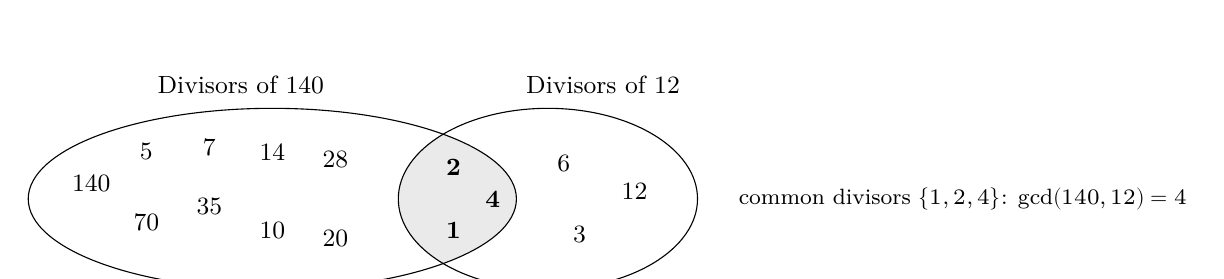
\begin{tikzpicture}[font=\small]
  \begin{scope}
    \clip (0,0) ellipse (3.1 and 1.15);
    \fill[gray!18] (3.5,0) ellipse (1.9 and 1.15);
  \end{scope}
  \draw (0,0) ellipse (3.1 and 1.15);
  \draw (3.5,0) ellipse (1.9 and 1.15);
  \node at (-0.4,1.45) {Divisors of 140};
  \node at (4.2,1.45) {Divisors of 12};
  \foreach \x/\y/\v in {-2.3/0.2/140,-1.6/0.6/5,-1.6/-0.3/70,-0.8/0.65/7,-0.8/-0.1/35,0/0.6/14,0/-0.4/10,0.8/0.5/28,0.8/-0.5/20}{\node at (\x,\y) {\v};}
  \foreach \x/\y/\v in {2.3/0.4/2,2.3/-0.4/1,2.8/0/4}{\node[font=\small\bfseries] at (\x,\y) {\v};}
  \foreach \x/\y/\v in {3.7/0.45/6,3.9/-0.45/3,4.6/0.1/12}{\node at (\x,\y) {\v};}
  \node[anchor=west] at (5.8,0) {\footnotesize common divisors $\{1, 2, 4\}$: $\gcd(140, 12) = 4$};
\end{tikzpicture}
\end{center}

\subsection{Euclid's algorithm and why it works}
The algorithm rests on two facts stated on the slides.
\[
\textbf{Fact 1: } \gcd(a, 0) = a, \qquad\qquad \textbf{Fact 2: } \gcd(a, b) = \gcd(b, r), \text{ where } r = a \bmod b .
\]
\textbf{Why Fact 1 holds.} Every integer divides 0 (since $0 = 0 \times d$), so the common divisors of $a$ and 0 are just the divisors of $a$, and the largest of these is $a$ itself.

\textbf{Why Fact 2 holds.} Divide: $a = qb + r$. If $d$ divides both $a$ and $b$, then by Property 4 it divides $a - qb = r$. Conversely, if $d$ divides both $b$ and $r$, then it divides $qb + r = a$. The pairs $(a, b)$ and $(b, r)$ therefore have exactly the same set of common divisors, and so the same greatest common divisor. The argument works for any multiple $qb$; the remainder is used because it makes the new pair as small as possible.

\textbf{The algorithm.} Apply Fact 2 repeatedly, replacing $(a, b)$ by $(b, a \bmod b)$, until the second number is 0; then Fact 1 gives the answer. The slide's example:
\[
\gcd(36, 10) = \gcd(10, 6) = \gcd(6, 4) = \gcd(4, 2) = \gcd(2, 0) = \mathbf{2}.
\]
\textbf{Termination.} Each step replaces the second number $b$ by $r = a \bmod b$, and $0 \le r < b$. The second numbers therefore form a strictly decreasing sequence of non-negative integers, $b > r_1 > r_2 > \cdots$, which must reach 0 after at most $b$ steps; the last non-zero term is the gcd.

\textbf{Speed.} The bound of $b$ steps is far too pessimistic: the remainder at least halves every two steps. Consider three consecutive remainders, where $r_{i+2} = r_i \bmod r_{i+1}$. If $r_{i+1} \le r_i / 2$, then $r_{i+2} < r_{i+1} \le r_i / 2$. Otherwise $r_{i+1} > r_i / 2$, the quotient is 1, and $r_{i+2} = r_i - r_{i+1} < r_i / 2$. Either way two steps halve the remainder, so at most about $2\log_2 b$ divisions are needed, which is linear in the number of digits. A 1024-bit $b$ therefore needs at most about 2048 divisions, while listing divisors would need about $2^{1024}$ trial divisions. The slowest inputs are consecutive Fibonacci numbers, where every quotient is 1: $\gcd(89, 55)$ takes 9 divisions.

Forouzan writes the algorithm with two variables $r_1$ and $r_2$ that hold the current pair:
\begin{center}
\begin{minipage}{0.55\textwidth}
\small\ttfamily
r$_1$ $\leftarrow$ a;\quad r$_2$ $\leftarrow$ b;\hfill\textrm{(initialisation)}\\
while (r$_2$ > 0)\\
\{\\
\hspace*{1.5em}q $\leftarrow$ r$_1$ / r$_2$;\hfill\textrm{(integer quotient)}\\
\hspace*{1.5em}r $\leftarrow$ r$_1$ $-$ q $\times$ r$_2$;\\
\hspace*{1.5em}r$_1$ $\leftarrow$ r$_2$;\quad r$_2$ $\leftarrow$ r;\\
\}\\
gcd(a, b) $\leftarrow$ r$_1$
\end{minipage}
\end{center}

\begin{mustknow}
$\gcd(a, b) = \gcd(b,\ a \bmod b)$ and $\gcd(a, 0) = a$. Divide, shift ($B \to A$, $R \to B$), and stop when the second number is 0: the gcd is the last non-zero remainder. At most about $2\log_2 b$ divisions.
\end{mustknow}

\subsection{Method 1: the table (Q, A, B, R)}
The lecture video lays the divisions out as a table, which is the format to use in an exam.
\begin{enumerate}[leftmargin=1.5em,itemsep=1pt]
  \item Draw the columns $Q$ (quotient), $A$, $B$ and $R$ (remainder), and start with $A$ = the larger number and $B$ = the smaller.
  \item In each row compute $Q = \lfloor A/B \rfloor$ and $R = A \bmod B$, so that $A = Q \times B + R$.
  \item In the next row $B$ moves into $A$ and $R$ moves into $B$ (the diagonal arrows below). This is Fact 2.
  \item Stop when $B = 0$, since division by 0 is impossible; write X for $Q$ and $R$. The gcd is the $A$ of that row (Fact 1).
\end{enumerate}
\begin{center}
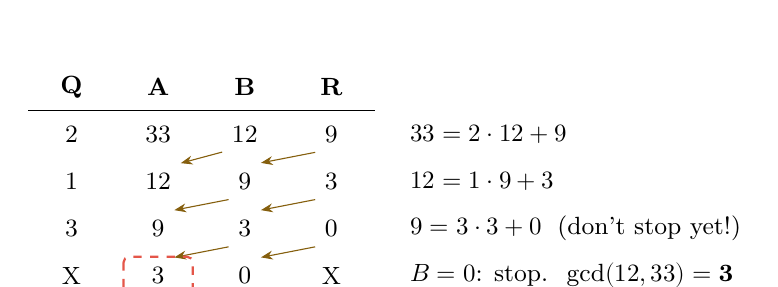
\begin{tikzpicture}[x=11mm,y=6mm]
  \foreach \h [count=\c] in {Q,A,B,R}{\node[font=\small\bfseries] at (\c,0) {\h};}
  \draw (0.5,-0.5) -- (4.5,-0.5);
  \foreach \q/\a/\b/\r [count=\i] in {2/33/12/9, 1/12/9/3, 3/9/3/0, X/3/0/X}{
    \node[font=\small] at (1,-\i) {\q};
    \node[font=\small] (a\i) at (2,-\i) {\a};
    \node[font=\small] (b\i) at (3,-\i) {\b};
    \node[font=\small] (r\i) at (4,-\i) {\r};
  }
  \foreach \i in {1,2,3}{\pgfmathtruncatemacro{\j}{\i+1}
    \draw[-{Stealth[length=1.5mm]},orange!80!black] (b\i.south west) -- (a\j.north east);
    \draw[-{Stealth[length=1.5mm]},orange!80!black] (r\i.south west) -- (b\j.north east);}
  \draw[warn,thick,dashed,rounded corners=2pt] (1.6,-3.6) rectangle (2.4,-4.4);
  \node[font=\small,anchor=west] at (4.8,-1) {$33 = 2\cdot12 + 9$};
  \node[font=\small,anchor=west] at (4.8,-2) {$12 = 1\cdot9 + 3$};
  \node[font=\small,anchor=west] at (4.8,-3) {$9 = 3\cdot3 + 0$ \;(don't stop yet!)};
  \node[font=\small,anchor=west] at (4.8,-4) {$B = 0$: stop. \;$\gcd(12, 33) = \mathbf{3}$};
\end{tikzpicture}
\end{center}
The other lecture examples, and Forouzan's slide example with the columns named $q, r_1, r_2, r$ (the same table under different names):
\begin{center}\small
\begin{minipage}[t]{0.27\textwidth}
\centering
$\gcd(750, 900)$\\[2pt]
\begin{tabular}{cccc}
\toprule
Q&A&B&R\\
\midrule
1&900&750&150\\
5&750&150&0\\
X&\textbf{150}&0&X\\
\bottomrule
\end{tabular}
\end{minipage}\hfill
\begin{minipage}[t]{0.27\textwidth}
\centering
$\gcd(252, 105)$\\[2pt]
\begin{tabular}{cccc}
\toprule
Q&A&B&R\\
\midrule
2&252&105&42\\
2&105&42&21\\
2&42&21&0\\
X&\textbf{21}&0&X\\
\bottomrule
\end{tabular}
\end{minipage}\hfill
\begin{minipage}[t]{0.36\textwidth}
\centering
$\gcd(2740, 1760)$ (Lecture 2)\\[2pt]
\begin{tabular}{cccc}
\toprule
$q$&$r_1$&$r_2$&$r$\\
\midrule
1&2740&1760&980\\
1&1760&980&780\\
1&980&780&200\\
3&780&200&180\\
1&200&180&20\\
9&180&20&0\\
&\textbf{20}&0&\\
\bottomrule
\end{tabular}
\end{minipage}
\end{center}
\textbf{Shortcut.} The gcd is the \textbf{last non-zero remainder} (9, 3, \textbf{3}, then 0; or 42, \textbf{21}, then 0). The extra row with $B = 0$ is only where the lecture reads it off. The Lecture 2 class exercise, $\gcd(25, 60)$, runs $60 = 2 \times 25 + 10$, $25 = 2 \times 10 + 5$, $10 = 2 \times 5 + 0$, giving $\mathbf{5}$.

\subsection{Method 2: recursion}
Facts 1 and 2 are already a recursive definition, and the second lecture video writes them as a function:
\begin{center}
\begin{minipage}{0.45\textwidth}
\small\ttfamily
Prerequisite: a > b\\
Euclid\_GCD(a, b):\\
\hspace*{1.5em}if b = 0 then\\
\hspace*{3em}return a;\hfill\textrm{(Fact 1)}\\
\hspace*{1.5em}else\\
\hspace*{3em}return Euclid\_GCD(b, a mod b);\hfill\textrm{(Fact 2)}
\end{minipage}
\end{center}
\begin{minipage}[t]{0.42\textwidth}
\small
\textbf{$\gcd(50, 12)$}\\
$= \gcd(12, 50 \bmod 12) = \gcd(12, 2)$\\
$= \gcd(2, 12 \bmod 2) = \gcd(2, 0)$\\
$= \mathbf{2}$
\end{minipage}\hfill
\begin{minipage}[t]{0.55\textwidth}
\small
\textbf{$\gcd(83, 19)$}\\
$= \gcd(19, 7)$ \quad ($83 = 4\cdot19 + 7$)\\
$= \gcd(7, 5)$ \quad ($19 = 2\cdot7 + 5$)\\
$= \gcd(5, 2)$ \quad ($7 = 1\cdot5 + 2$)\\
$= \gcd(2, 1)$ \quad ($5 = 2\cdot2 + 1$)\\
$= \gcd(1, 0) = \mathbf{1}$ \quad ($2 = 2\cdot1 + 0$)
\end{minipage}

\medskip
Both methods perform exactly the same divisions, so either may be used. The prerequisite $a > b$ is a convenience, not a necessity. If the smaller number comes first, the first call swaps them at the cost of one wasted step: $\gcd(12, 33) \to \gcd(33, 12 \bmod 33) = \gcd(33, 12)$, since $12 \bmod 33 = 12$. In the exam it is cleaner to write the larger number first.

\subsection{Relatively prime numbers}
\imp{Two integers $a$ and $b$ are relatively prime (co-prime) if $\gcd(a, b) = 1$}, as for 83 and 19 above. The condition is about the pair: neither number has to be prime, as $\gcd(8, 9) = 1$ shows. Cryptography needs the notion for three reasons. First, $a^{-1} \bmod n$ exists only if $\gcd(a, n) = 1$ (\S\ref{sec:modular}); this is the Hill key condition $\gcd(\det K, 26) = 1$ and the affine-cipher condition on the multiplier. Second, RSA key generation chooses $e$ with $\gcd(e, \phi(n)) = 1$, so that $d = e^{-1} \bmod \phi(n)$ exists. Third, the number of residues co-prime to $n$ is Euler's totient $\phi(n)$ (\S\ref{sec:totient}). Euclid's algorithm decides co-primality; the extended algorithm (\S\ref{sec:exteuclid}) runs the same divisions while tracking two extra columns and produces the inverse itself, instead of the trial-and-error table used for $23^{-1} \bmod 26$ in the Hill cipher.

\begin{worked}[: GCD by the Euclidean algorithm (Forouzan exercise)]
\textbf{Q.} Find (a) $\gcd(88, 220)$ \quad (b) $\gcd(300, 42)$ \quad (c) $\gcd(24, 320)$ \quad (d) $\gcd(401, 700)$. Which pairs are relatively prime?

\textbf{A.} Larger number first; each line is one row $A = Q \times B + R$.
\begin{center}\small
\begin{tabular}{@{}lll@{}}
\toprule
Pair & Divisions & gcd\\
\midrule
(a) 220, 88 & $220 = 2 \times 88 + 44$, \;$88 = 2 \times 44 + 0$ & \textbf{44}\\
(b) 300, 42 & $300 = 7 \times 42 + 6$, \;$42 = 7 \times 6 + 0$ & \textbf{6}\\
(c) 320, 24 & $320 = 13 \times 24 + 8$, \;$24 = 3 \times 8 + 0$ & \textbf{8}\\
\bottomrule
\end{tabular}
\end{center}
(d) needs a longer table:
\begin{center}\small
\begin{tabular}{cccc|l}
\toprule
Q&A&B&R&\\
\midrule
1&700&401&299&$700 = 1 \times 401 + 299$\\
1&401&299&102&$401 = 1 \times 299 + 102$\\
2&299&102&95&$299 = 2 \times 102 + 95$\\
1&102&95&7&$102 = 1 \times 95 + 7$\\
13&95&7&4&$95 = 13 \times 7 + 4$\\
1&7&4&3&$7 = 1 \times 4 + 3$\\
1&4&3&1&$4 = 1 \times 3 + 1$\\
3&3&1&0&$3 = 3 \times 1 + 0$\\
X&\textbf{1}&0&X&\\
\bottomrule
\end{tabular}
\end{center}
\textbf{Answers: 44, 6, 8, 1.} Only 401 and 700 are relatively prime, so 401 has an inverse modulo 700 and the other pairs have none. \textbf{Check:} $88 = 2 \times 44$ and $220 = 5 \times 44$ with $\gcd(2, 5) = 1$; similarly $300 = 50 \times 6$, $42 = 7 \times 6$ and $320 = 40 \times 8$, $24 = 3 \times 8$, with co-prime cofactors.
\end{worked}

\textbf{Lecture homework:} $\gcd(1005, 105)$ (table method) and $\gcd(529, 123)$ (recursive method). Solutions are in practice Q43.

\begin{trap}[: reading the table]
\begin{itemize}[leftmargin=1.5em]
  \item Stop when $B = 0$, not when $R = 0$. In the row where $R$ first becomes 0, the answer is that row's $B$, which moves into $A$ in the next row; reading $A$ from the row with $R = 0$ gives a wrong answer (9 instead of 3 for $\gcd(33, 12)$).
  \item Swapping the meaning of the two outputs: ``$A \bmod B$'' gives the remainder $R$, while ``$A$ divided by $B$'' gives the quotient $Q$. The table needs both.
  \item Show every division as $A = Q \times B + R$ in the exam; the marks are for the steps, not only for the final number.
\end{itemize}
\end{trap}

\begin{fixbox}
\begin{itemize}
  \item All results are correct (checked by script): 3, 25, 1, 3, 150, 21, 2, 1 from the videos, and $\gcd(36, 10) = 2$, $\gcd(2740, 1760) = 20$, $\gcd(25, 60) = 5$, $\gcd(140, 12) = 4$ from the Lecture 2 slides.
  \item Verbal slips only: ``divisors of 13'' means 33 (video 1); ``a = 9'' means 19 (video 2). The slides are right.
  \item Wording: ``$A$ mod $B$'' gives the \emph{remainder}; ``$A$ divided by $B$'' gives the quotient $Q$. The table needs both.
\end{itemize}
\end{fixbox}

% College Lecture 2 (extended Euclid: process, algorithm, 161/28, 17/0, 0/45, 84/320) + Lecture 4 (inverse with the t columns,
% 11/26, 23/100, 12/26; linear Diophantine equations), Forouzan 2.1--2.2. All tables generated by script (scratchpad/r4/verify.py).
\section{Extended Euclidean Algorithm \hothot}\label{sec:exteuclid}
\asked{Mid-sem 2024--25 Q7 (5 marks): pseudocode + $23^{-1}$ in $\mathbb{Z}_{100}$ with ``value in iteration $k$'' sub-questions. 2025--26 Q5 (3 marks): solve $19x + 13y = 20$. The same table, with polynomials, gives the GF$(2^8)$ inverse asked in both years (\S\ref{sec:algebra}), and $d$ in RSA (\S\ref{sec:rsa}).}

Euclid's algorithm decides whether $\gcd(a, n) = 1$, and hence whether $a^{-1} \bmod n$ exists, but it does not produce the inverse. The extended Euclidean algorithm does. \imp{Given two integers $a$ and $b$, the extended Euclidean algorithm computes $\gcd(a, b)$ and, at the same time, integers $s$ and $t$ such that $s \times a + t \times b = \gcd(a, b)$.} That such $s$ and $t$ always exist is \textbf{Bézout's identity}; the algorithm proves it by constructing them. One table then answers four kinds of exam question: the inverse $b^{-1} \bmod n$, the solutions of a linear Diophantine equation $ax + by = c$, the solutions of a linear congruence (\S\ref{sec:modular}), and the RSA private key $d = e^{-1} \bmod \phi(n)$. With polynomials instead of integers the same table gives inverses in GF$(2^8)$.

\subsection{The idea: carry every remainder as a combination of \texorpdfstring{$a$ and $b$}{a and b}}
By hand, $s$ and $t$ can be found by back-substitution. For $a = 19$ and $b = 13$, Euclid's divisions are $19 = 1 \times 13 + 6$ and $13 = 2 \times 6 + 1$. Solving them from the last line upwards gives
\[
1 = 13 - 2 \times 6 = 13 - 2 \times (19 - 1 \times 13) = 3 \times 13 - 2 \times 19,
\]
so $s = -2$ and $t = 3$. This works, but it requires storing every quotient, running the divisions a second time in reverse, and keeping track of signs, which is where most errors happen. The extended algorithm does the same bookkeeping forwards, in a single pass.

The key observation is that every remainder in Euclid's sequence is an integer combination of $a$ and $b$. The first two numbers of the sequence are $a$ and $b$ themselves, and trivially
\[
r_1 = a = 1 \cdot a + 0 \cdot b, \qquad r_2 = b = 0 \cdot a + 1 \cdot b,
\]
which gives the starting values $s_1 = 1$, $s_2 = 0$, $t_1 = 0$, $t_2 = 1$. Suppose that in some row the \textbf{invariant} $r_1 = s_1 a + t_1 b$ and $r_2 = s_2 a + t_2 b$ holds. The next remainder is $r = r_1 - q r_2$, and substituting the two combinations gives
\[
r = (s_1 a + t_1 b) - q\,(s_2 a + t_2 b) = (s_1 - q s_2)\,a + (t_1 - q t_2)\,b .
\]
So if $s$ and $t$ are updated by exactly the same rule as $r$, namely $s = s_1 - q s_2$ and $t = t_1 - q t_2$, the new remainder satisfies $r = s a + t b$. After the shift $(r_1, r_2) \leftarrow (r_2, r)$, $(s_1, s_2) \leftarrow (s_2, s)$, $(t_1, t_2) \leftarrow (t_2, t)$ the invariant holds again, so by induction it holds in every row. The $r$ columns are Euclid's algorithm unchanged, so the loop ends with $r_1 = \gcd(a, b)$ and $r_2 = 0$, and the invariant for $r_1$ then reads $\gcd(a, b) = s_1 a + t_1 b$. This proves Bézout's identity for all $a$ and $b$.

\subsection{The algorithm and the table (Forouzan)}
The slides give the algorithm as three identical update blocks, one for each pair of variables:
\begin{center}
\begin{minipage}{0.62\textwidth}
\small\ttfamily
r$_1$ $\leftarrow$ a;\quad r$_2$ $\leftarrow$ b;\\
s$_1$ $\leftarrow$ 1;\quad s$_2$ $\leftarrow$ 0;\hfill\textrm{(initialisation)}\\
t$_1$ $\leftarrow$ 0;\quad t$_2$ $\leftarrow$ 1;\\
while (r$_2$ > 0)\\
\{\\
\hspace*{1.5em}q $\leftarrow$ r$_1$ / r$_2$;\\
\hspace*{1.5em}r $\leftarrow$ r$_1$ $-$ q $\times$ r$_2$;\quad r$_1$ $\leftarrow$ r$_2$;\quad r$_2$ $\leftarrow$ r;\hfill\textrm{(updating r's)}\\
\hspace*{1.5em}s $\leftarrow$ s$_1$ $-$ q $\times$ s$_2$;\quad s$_1$ $\leftarrow$ s$_2$;\quad s$_2$ $\leftarrow$ s;\hfill\textrm{(updating s's)}\\
\hspace*{1.5em}t $\leftarrow$ t$_1$ $-$ q $\times$ t$_2$;\quad t$_1$ $\leftarrow$ t$_2$;\quad t$_2$ $\leftarrow$ t;\hfill\textrm{(updating t's)}\\
\}\\
gcd(a, b) $\leftarrow$ r$_1$;\quad s $\leftarrow$ s$_1$;\quad t $\leftarrow$ t$_1$
\end{minipage}
\end{center}
On paper each pass of the loop is one row of a table with the columns $q \mid r_1\ r_2\ r \mid s_1\ s_2\ s \mid t_1\ t_2\ t$. In every row the three blocks do the same thing: the new value is (first) $-\ q \times$ (second), and in the next row the second value moves into the first column and the new value into the second. A final row, with no quotient, shows the values after the loop, and the answer is read from its \emph{first} columns. The slide example, $a = 161$, $b = 28$:
\begin{center}\small
\begin{tabular}{@{}r|rrr|rrr|rrr@{}}
\toprule
$q$ & $r_1$ & $r_2$ & $r$ & $s_1$ & $s_2$ & $s$ & $t_1$ & $t_2$ & $t$\\
\midrule
5 & 161 & 28 & 21 & 1 & 0 & 1 & 0 & 1 & $-5$\\
1 & 28 & 21 & 7 & 0 & 1 & $-1$ & 1 & $-5$ & 6\\
3 & 21 & 7 & 0 & 1 & $-1$ & 4 & $-5$ & 6 & $-23$\\
 & \textbf{7} & 0 & & $\mathbf{-1}$ & 4 & & \textbf{6} & $-23$ & \\
\bottomrule
\end{tabular}
\end{center}
$\gcd(161, 28) = 7$, $s = -1$, $t = 6$: \;$(-1)(161) + 6(28) = -161 + 168 = 7$ \checkmark. The invariant can be checked in every row: $21 = 1 \times 161 - 5 \times 28$, $7 = -1 \times 161 + 6 \times 28$ and $0 = 4 \times 161 - 23 \times 28$. The last of these gives a free self-check: in the final row $s_2 a + t_2 b = 0$, and $(s_2, t_2)$ always equals $\pm(b/d, -a/d)$ with $d = \gcd(a, b)$; here $(4, -23) = (28/7, -161/7)$. In an inverse table (next subsection) this means the final $t_2$ is $\pm n$, so any other value there reveals an arithmetic slip.

The other slide examples test the edge cases. For $a = 17$, $b = 0$ the loop never runs, because $r_2 = 0$ from the start, and the initial values give $\gcd(17, 0) = 17$, $s = 1$, $t = 0$. For $a = 0$, $b = 45$ one iteration with $q = 0$ swaps the pair, giving $\gcd(0, 45) = 45$, $s = 0$, $t = 1$. The slide exercise $a = 84$, $b = 320$ also starts with the smaller number, and the first row ($q = 0$) simply swaps it:
\begin{center}\small
\begin{tabular}{@{}r|rrr|rrr|rrr@{}}
\toprule
$q$ & $r_1$ & $r_2$ & $r$ & $s_1$ & $s_2$ & $s$ & $t_1$ & $t_2$ & $t$\\
\midrule
0 & 84 & 320 & 84 & 1 & 0 & 1 & 0 & 1 & 0\\
3 & 320 & 84 & 68 & 0 & 1 & $-3$ & 1 & 0 & 1\\
1 & 84 & 68 & 16 & 1 & $-3$ & 4 & 0 & 1 & $-1$\\
4 & 68 & 16 & 4 & $-3$ & 4 & $-19$ & 1 & $-1$ & 5\\
4 & 16 & 4 & 0 & 4 & $-19$ & 80 & $-1$ & 5 & $-21$\\
 & \textbf{4} & 0 & & $\mathbf{-19}$ & 80 & & \textbf{5} & $-21$ & \\
\bottomrule
\end{tabular}
\end{center}
$\gcd(84, 320) = 4$, $s = -19$, $t = 5$: \;$-19 \times 84 + 5 \times 320 = -1596 + 1600 = 4$ \checkmark, as on the slide. The final $(s_2, t_2) = (80, -21) = (320/4, -84/4)$ confirms it.

\subsection{Multiplicative inverse with the table \hothot}
\likely{``Find $b^{-1}$ in $\mathbb{Z}_n$ using the extended Euclidean algorithm; give the number of iterations / $r$ or $t$ in iteration $k$'' (5 marks), and $d = e^{-1} \bmod \phi(n)$ in every RSA question.}
To find $b^{-1} \bmod n$, run the algorithm with $a = n$, that is, $r_1 = n$ and $r_2 = b$. At the end $s \times n + t \times b = \gcd(n, b)$. If the gcd is 1, reduce this equation modulo $n$; the slides do it in three lines:
\[
(s \times n + b \times t) \bmod n = 1 \;\Rightarrow\; [(s \times n) \bmod n] + [(b \times t) \bmod n] = 1 \;\Rightarrow\; (b \times t) \bmod n = 1 .
\]
So \imp{the multiplicative inverse of $b$ is the final $t_1$, mapped into $\mathbb{Z}_n$}. The $s$ columns are never used and are dropped, leaving $q \mid r_1\ r_2\ r \mid t_1\ t_2\ t$. If the final $r_1$ is not 1, then $\gcd(n, b) > 1$ and no inverse exists (\S\ref{sec:modular}); the algorithm detects this by itself. A negative $t_1$ is normal and is mapped into $\mathbb{Z}_n$ by adding $n$. The slide's version of the algorithm, which is the pseudocode asked in 2024--25 Q7:
\begin{center}
\begin{minipage}{0.56\textwidth}
\small\ttfamily
r$_1$ $\leftarrow$ n;\quad r$_2$ $\leftarrow$ b;\quad t$_1$ $\leftarrow$ 0;\quad t$_2$ $\leftarrow$ 1;\\
while (r$_2$ > 0)\\
\{\\
\hspace*{1.5em}q $\leftarrow$ r$_1$ / r$_2$;\\
\hspace*{1.5em}r $\leftarrow$ r$_1$ $-$ q $\times$ r$_2$;\quad r$_1$ $\leftarrow$ r$_2$;\quad r$_2$ $\leftarrow$ r;\\
\hspace*{1.5em}t $\leftarrow$ t$_1$ $-$ q $\times$ t$_2$;\quad t$_1$ $\leftarrow$ t$_2$;\quad t$_2$ $\leftarrow$ t;\\
\}\\
if (r$_1$ = 1) then b$^{-1}$ $\leftarrow$ t$_1$ mod n\\
else ``no inverse''
\end{minipage}
\end{center}
The three slide examples:
\begin{center}\small
\begin{tabular}{@{}r|rrr|rrr@{}}
\multicolumn{7}{c}{$11^{-1} \bmod 26$}\\
\toprule
$q$ & $r_1$ & $r_2$ & $r$ & $t_1$ & $t_2$ & $t$\\
\midrule
2 & 26 & 11 & 4 & 0 & 1 & $-2$\\
2 & 11 & 4 & 3 & 1 & $-2$ & 5\\
1 & 4 & 3 & 1 & $-2$ & 5 & $-7$\\
3 & 3 & 1 & 0 & 5 & $-7$ & 26\\
 & \textbf{1} & 0 & & $\mathbf{-7}$ & 26 & \\
\bottomrule
\end{tabular}
\quad
\begin{tabular}{@{}r|rrr|rrr@{}}
\multicolumn{7}{c}{$23^{-1} \bmod 100$}\\
\toprule
$q$ & $r_1$ & $r_2$ & $r$ & $t_1$ & $t_2$ & $t$\\
\midrule
4 & 100 & 23 & 8 & 0 & 1 & $-4$\\
2 & 23 & 8 & 7 & 1 & $-4$ & 9\\
1 & 8 & 7 & 1 & $-4$ & 9 & $-13$\\
7 & 7 & 1 & 0 & 9 & $-13$ & 100\\
 & \textbf{1} & 0 & & $\mathbf{-13}$ & 100 & \\
\bottomrule
\end{tabular}
\quad
\begin{tabular}{@{}r|rrr|rrr@{}}
\multicolumn{7}{c}{$12^{-1} \bmod 26$}\\
\toprule
$q$ & $r_1$ & $r_2$ & $r$ & $t_1$ & $t_2$ & $t$\\
\midrule
2 & 26 & 12 & 2 & 0 & 1 & $-2$\\
6 & 12 & 2 & 0 & 1 & $-2$ & 13\\
 & \textbf{2} & 0 & & $-2$ & 13 & \\
\bottomrule
\end{tabular}
\end{center}
$11^{-1} \equiv -7 \equiv \mathbf{19} \pmod{26}$ (check: $11 \times 19 = 209 = 8 \times 26 + 1$); \;$23^{-1} \equiv -13 \equiv \mathbf{87} \pmod{100}$ (check: $23 \times 87 = 2001$); \;$12^{-1} \bmod 26$: the final $r_1 = 2$, so $\gcd(26, 12) = 2$ and \textbf{no inverse exists}. In the third table $t_1 = -2$ still satisfies $12 \times (-2) \equiv 2 \pmod{26}$, the gcd rather than 1, which is exactly what the invariant predicts.

\begin{worked}[: 2024--25 Q7 (5 marks), inverse with ``iteration $k$'' sub-questions]
\textbf{Q.} Write the pseudocode for finding the multiplicative inverse of $b$ in $\mathbb{Z}_n$, and use it to find $23^{-1}$ in $\mathbb{Z}_{100}$. State (a) the number of iterations, (b) the remainder in iteration 2, (c) the value of $t$ in iteration 4, (d) the iteration whose $t$ becomes the inverse.

\textbf{A.} Pseudocode: as above ($r_1 = n$, $r_2 = b$, $t_1 = 0$, $t_2 = 1$; loop while $r_2 > 0$; inverse $= t_1 \bmod n$ if $r_1 = 1$). An \emph{iteration} is one pass of the while loop, i.e.\ one row that has a quotient; the row shows the values at the start of the pass and the $r$, $t$ computed in it.
\begin{center}\small
\begin{tabular}{@{}c|c|rrr|rrr@{}}
\toprule
Iteration & $q$ & $r_1$ & $r_2$ & $r$ & $t_1$ & $t_2$ & $t$\\
\midrule
1 & 4 & 100 & 23 & 8 & 0 & 1 & $-4$\\
2 & 2 & 23 & 8 & \textbf{7} & 1 & $-4$ & 9\\
3 & 1 & 8 & 7 & 1 & $-4$ & 9 & $\mathbf{-13}$\\
4 & 7 & 7 & 1 & 0 & 9 & $-13$ & \textbf{100}\\
(end) & & \textbf{1} & 0 & & $\mathbf{-13}$ & 100 & \\
\bottomrule
\end{tabular}
\end{center}
Since $r_1 = 1$, $\gcd(100, 23) = 1$ and the inverse exists. (a) \textbf{4 iterations}. (b) The remainder in iteration 2 is $\mathbf{7}$ ($23 = 2 \times 8 + 7$). (c) $t$ in iteration 4 is $\mathbf{100}$, which is $\pm n$ as the self-check predicts. (d) Iteration 3 computes $t = -13$, which becomes the final $t_1$; mapped into $\mathbb{Z}_{100}$: $23^{-1} = -13 + 100 = \mathbf{87}$.
\textbf{Check:} $23 \times 87 = 2001 = 20 \times 100 + 1$ \checkmark.
\end{worked}

\begin{worked}[: inverse in $\mathbb{Z}_{180}$ (Forouzan exercise)]
\textbf{Q.} Using the extended Euclidean algorithm, find the multiplicative inverses of 7, 132 and 24 in $\mathbb{Z}_{180}$, where they exist.

\textbf{A.} For $b = 7$:
\begin{center}\small
\begin{tabular}{@{}c|c|rrr|rrr@{}}
\toprule
Iteration & $q$ & $r_1$ & $r_2$ & $r$ & $t_1$ & $t_2$ & $t$\\
\midrule
1 & 25 & 180 & 7 & 5 & 0 & 1 & $-25$\\
2 & 1 & 7 & 5 & 2 & 1 & $-25$ & 26\\
3 & 2 & 5 & 2 & 1 & $-25$ & 26 & $-77$\\
4 & 2 & 2 & 1 & 0 & 26 & $-77$ & 180\\
(end) & & \textbf{1} & 0 & & $\mathbf{-77}$ & 180 & \\
\bottomrule
\end{tabular}
\end{center}
$r_1 = 1$, so the inverse exists: $7^{-1} = -77 + 180 = \mathbf{103}$. Check: $7 \times 103 = 721 = 4 \times 180 + 1$ \checkmark.
For $b = 132$ the $r$ columns run $180 = 1 \times 132 + 48$, $132 = 2 \times 48 + 36$, $48 = 1 \times 36 + 12$, $36 = 3 \times 12 + 0$, ending with $r_1 = 12 \ne 1$: \textbf{no inverse}. For $b = 24$: $180 = 7 \times 24 + 12$, $24 = 2 \times 12 + 0$, again $r_1 = 12$: \textbf{no inverse}. Both share the factor 12 with 180.
\end{worked}

\subsection{Linear Diophantine equations \texorpdfstring{$ax + by = c$}{ax + by = c} \hot}
\likely{``Find the particular and general solutions of $ax + by = c$'' (3 marks), as in 2025--26 Q5; occasionally a word problem with non-negative solutions.}
\imp{A linear Diophantine equation in two variables is $ax + by = c$, where $a$, $b$, $c$ are integers and only integer solutions $x$, $y$ are wanted.} Over the reals such an equation has a whole line of solutions; restricting to integers leaves either none or infinitely many, and the extended Euclidean algorithm decides which and finds them all. The three facts below are derived from Bézout's identity, with $d = \gcd(a, b)$.

\textbf{No solution unless $d \mid c$.} For every pair of integers $x, y$, $d$ divides $ax + by$ (Property 4 of \S\ref{sec:gcd}). If $d \nmid c$, no choice of $x$, $y$ can make $ax + by$ equal to $c$. For example $15x + 12y = 13$ has no solution, because $\gcd(15, 12) = 3$ and $3 \nmid 13$.

\textbf{A particular solution when $d \mid c$.} Divide the equation by $d$: $a'x + b'y = c'$ with $a' = a/d$, $b' = b/d$, $c' = c/d$ and $\gcd(a', b') = 1$. The extended algorithm on $(a', b')$ gives $s$ and $t$ with $a's + b't = 1$, and multiplying by $c'$ gives $a'(c's) + b'(c't) = c'$. So $x_0 = (c/d)\,s$, $y_0 = (c/d)\,t$ is a solution. (Running the algorithm on $(a, b)$ directly gives the same $s$, $t$, since $sa + tb = d$ is the same equation multiplied by $d$.)

\textbf{The general solution.} Let $(x, y)$ be any other solution. Subtracting $a'x_0 + b'y_0 = c'$ from $a'x + b'y = c'$ gives $a'(x - x_0) = b'(y_0 - y)$. So $b'$ divides $a'(x - x_0)$, and since $b'$ is co-prime to $a'$, it divides $x - x_0$. (This step, \emph{Euclid's lemma}, follows from Bézout as well: multiplying $a's + b't = 1$ by $m = x - x_0$ gives $m = s\,a'm + t\,b'm$, and $b'$ divides both terms.) Hence $x = x_0 + k b'$ for some integer $k$, and substituting back gives $y = y_0 - k a'$. Conversely every $k$ gives a solution, because $a'(x_0 + kb') + b'(y_0 - ka') = a'x_0 + b'y_0$. These are the slide's formulas:
\[
\text{particular: } x_0 = \frac{c}{d}\,s, \quad y_0 = \frac{c}{d}\,t, \qquad\qquad
\text{general: } x = x_0 + k\,\frac{b}{d}, \quad y = y_0 - k\,\frac{a}{d}, \quad k \in \mathbb{Z}.
\]
The solutions are evenly spaced: $x$ steps by $b/d$ while $y$ steps by $a/d$ in the opposite direction, which keeps $ax + by$ constant. The linear congruence $ax \equiv b \pmod n$ of \S\ref{sec:modular} is the same problem in disguise, since it means $ax + ny = b$ for some integer $y$; the condition $d \mid b$ and the spacing $n/d$ of its $d$ solutions are this result read modulo $n$.

\begin{mustknow}
$s \cdot a + t \cdot b = \gcd(a, b)$: update $r$, $s$, $t$ by the same rule (new $=$ first $- q \times$ second), stop when $r_2 = 0$, read $r_1$, $s_1$, $t_1$.
Inverse: run with $r_1 = n$, $r_2 = b$; if the final $r_1 = 1$, then $b^{-1} = t_1 \bmod n$, otherwise no inverse.
$ax + by = c$: solvable iff $d = \gcd(a, b) \mid c$; $x = \frac{c}{d}s + k\frac{b}{d}$, \;$y = \frac{c}{d}t - k\frac{a}{d}$.
\end{mustknow}

The slide examples. For $21x + 14y = 35$: $d = \gcd(21, 14) = 7$ and $7 \mid 35$, so there are infinitely many solutions. Dividing by 7 gives $3x + 2y = 5$, and the algorithm on $(3, 2)$ gives $s = 1$, $t = -1$. The particular solution is $x_0 = 5 \times 1 = 5$, $y_0 = 5 \times (-1) = -5$, and the general solution is $x = 5 + 2k$, $y = -5 - 3k$: $(5, -5), (7, -8), (9, -11), \dots$, each of which satisfies $21x + 14y = 35$.
For cashing a Rs.~100 cheque in Rs.~20 and Rs.~5 notes, $20x + 5y = 100$: $d = 5$ divides 100, the reduced equation is $4x + y = 20$, and $4s + t = 1$ gives $s = 0$, $t = 1$. The particular solution is $x_0 = 0 \times 20 = 0$, $y_0 = 1 \times 20 = 20$, and the general one is $x = k$, $y = 20 - 4k$. Only non-negative note counts make sense, so $0 \le k \le 5$: $(0, 20)$, $(1, 16)$, $(2, 12)$, $(3, 8)$, $(4, 4)$, $(5, 0)$.

\begin{worked}[: 2025--26 Q5 (3 marks), solve $19x + 13y = 20$]
\textbf{Q.} Find the particular and general solutions of $19x + 13y = 20$.

\textbf{A.} Run the extended Euclidean algorithm on $a = 19$, $b = 13$:
\begin{center}\small
\begin{tabular}{@{}r|rrr|rrr|rrr@{}}
\toprule
$q$ & $r_1$ & $r_2$ & $r$ & $s_1$ & $s_2$ & $s$ & $t_1$ & $t_2$ & $t$\\
\midrule
1 & 19 & 13 & 6 & 1 & 0 & 1 & 0 & 1 & $-1$\\
2 & 13 & 6 & 1 & 0 & 1 & $-2$ & 1 & $-1$ & 3\\
6 & 6 & 1 & 0 & 1 & $-2$ & 13 & $-1$ & 3 & $-19$\\
 & \textbf{1} & 0 & & $\mathbf{-2}$ & 13 & & \textbf{3} & $-19$ & \\
\bottomrule
\end{tabular}
\end{center}
$d = \gcd(19, 13) = 1$, $s = -2$, $t = 3$ (check: $-2 \times 19 + 3 \times 13 = -38 + 39 = 1$). Since $1 \mid 20$, solutions exist.

\textbf{Particular:} $x_0 = (c/d)\,s = 20 \times (-2) = \mathbf{-40}$, \;$y_0 = (c/d)\,t = 20 \times 3 = \mathbf{60}$. \;Check: $19(-40) + 13(60) = -760 + 780 = 20$ \checkmark.

\textbf{General:} $x = -40 + 13k$, \;$y = 60 - 19k$, \;$k \in \mathbb{Z}$.
\begin{center}\small
\begin{tabular}{@{}c|cccccc@{}}
\toprule
$k$ & 0 & 1 & 2 & 3 & 4 & 5\\
\midrule
$(x, y)$ & $(-40, 60)$ & $(-27, 41)$ & $(-14, 22)$ & $\mathbf{(-1, 3)}$ & $(12, -16)$ & $(25, -35)$\\
\bottomrule
\end{tabular}
\end{center}
The smallest solution is $(-1, 3)$ ($k = 3$), so the general solution can also be written $x = -1 + 13k$, $y = 3 - 19k$. Check: $19(-1) + 13(3) = -19 + 39 = 20$ \checkmark.
\end{worked}

\begin{worked}[: non-negative solutions (Forouzan-style word problem)]
\textbf{Q.} A post office sells only 39-cent and 15-cent stamps. Find the numbers of stamps a customer can buy to pay exactly \$2.70 of postage.

\textbf{A.} Let $x$ and $y$ be the numbers of 39-cent and 15-cent stamps: $39x + 15y = 270$, with $x, y \ge 0$. $d = \gcd(39, 15) = 3$ ($39 = 2 \times 15 + 9$, $15 = 1 \times 9 + 6$, $9 = 1 \times 6 + 3$, $6 = 2 \times 3$), and $3 \mid 270$. Dividing by 3: $13x + 5y = 90$.
\begin{center}\small
\begin{tabular}{@{}r|rrr|rrr|rrr@{}}
\toprule
$q$ & $r_1$ & $r_2$ & $r$ & $s_1$ & $s_2$ & $s$ & $t_1$ & $t_2$ & $t$\\
\midrule
2 & 13 & 5 & 3 & 1 & 0 & 1 & 0 & 1 & $-2$\\
1 & 5 & 3 & 2 & 0 & 1 & $-1$ & 1 & $-2$ & 3\\
1 & 3 & 2 & 1 & 1 & $-1$ & 2 & $-2$ & 3 & $-5$\\
2 & 2 & 1 & 0 & $-1$ & 2 & $-5$ & 3 & $-5$ & 13\\
 & \textbf{1} & 0 & & \textbf{2} & $-5$ & & $\mathbf{-5}$ & 13 & \\
\bottomrule
\end{tabular}
\end{center}
$s = 2$, $t = -5$ ($2 \times 13 - 5 \times 5 = 1$). Particular: $x_0 = 90 \times 2 = 180$, $y_0 = 90 \times (-5) = -450$. General: $x = 180 + 5k$, $y = -450 - 13k$.
Non-negative counts need $180 + 5k \ge 0$, i.e.\ $k \ge -36$, and $-450 - 13k \ge 0$, i.e.\ $k \le -34.6$, so $k \in \{-36, -35\}$.
\textbf{Answer: $(x, y) = (0, 18)$ or $(5, 5)$}: eighteen 15-cent stamps, or five of each. Check: $15 \times 18 = 270$ and $39 \times 5 + 15 \times 5 = 195 + 75 = 270$ \checkmark.
\end{worked}

\begin{trap}[: where marks are lost]
\begin{itemize}[leftmargin=1.5em]
  \item For an inverse, put the \textbf{modulus first} ($r_1 = n$). Starting with $r_1 = b$ makes the inverse appear in the $s$ column, which the $t$-only table has dropped.
  \item Read the answer from the final row's \emph{first} columns ($r_1$, $s_1$, $t_1$), not from $t_2$ (which is $\pm n$) or from the last computed $t$.
  \item A negative $t_1$ is not an error: add $n$ (in RSA, add $\phi(n)$, never $n$). Check $b \times b^{-1} \bmod n = 1$ before writing the answer.
  \item If the final $r_1 \ne 1$, write ``no inverse, since $\gcd = r_1$''; do not report $t_1$.
  \item Show the full table with headed columns; the marks are awarded per row, and the ``iteration $k$'' sub-questions can only be answered from it.
\end{itemize}
\end{trap}

\begin{fixbox}
\begin{itemize}
  \item All slide tables are correct (recomputed by script): $(161, 28) \to 7, -1, 6$; $(17, 0) \to 17, 1, 0$; $(0, 45) \to 45, 0, 1$; $(84, 320) \to 4, -19, 5$; $11^{-1} \bmod 26 = 19$; $23^{-1} \bmod 100 = 87$; $12^{-1} \bmod 26$ does not exist; $21x + 14y = 35$ and the cheque solutions.
  \item Lecture 4, Diophantine slide: ``if $d \nmid c$, the equation has no solution'' has the ``not'' stroke hand-drawn on the slide. A text copy of the older slides lost it and reads ``if $d \mid c$, the equation has no solution'', which is wrong; the condition for \emph{no} solution is $d \nmid c$.
\end{itemize}
\end{fixbox}

% Lecture 4 (Z_n*), Lecture 10 (Euler's phi-function) + videos. All numbers recomputed by script (scratchpad/euler/verify.py).
\section{Relatively Prime Numbers, Euler's Totient and $\mathbb{Z}_n^*$}\label{sec:totient}

\subsection{Relatively prime (co-prime) numbers}
Two positive integers $a$ and $b$ are \imp{relatively prime (co-prime) if $\gcd(a, b) = 1$}, that is, if their only common positive divisor is 1. Neither number has to be prime: the condition is about the pair, not about each number. Since $12 = 2^2 \cdot 3$ and $77 = 7 \cdot 11$ share no prime factor, they are co-prime although both are composite, while $15 = 3 \cdot 5$ and $21 = 3 \cdot 7$ are not, because 3 divides both. If $p$ is prime, every integer from 1 to $p - 1$ is co-prime to $p$, since the only divisors of $p$ are 1 and $p$ itself.

Cryptography cares about this property for one reason: \textbf{$a$ has a multiplicative inverse modulo $n$ exactly when $\gcd(a, n) = 1$}. If $ax \equiv 1 \pmod n$, then $ax - kn = 1$ for some integer $k$, so any common divisor of $a$ and $n$ divides 1. Conversely, if $\gcd(a, n) = 1$, the extended Euclidean algorithm (\S\ref{sec:exteuclid}) produces $s, t$ with $sa + tn = 1$, and reducing modulo $n$ gives $sa \equiv 1$. Co-primality is therefore always checked with the Euclidean algorithm, never by eye.
\begin{center}\small
\begin{tabular}{@{}lllcl@{}}
\toprule
$a$, $b$ & Divisors / Euclid steps & GCD & Co-prime? & Note\\
\midrule
4, 13 & $\{1,2,4\}$, $\{1,13\}$ & 1 & yes & composite + prime\\
15, 21 & $\{1,3,5,15\}$, $\{1,3,7,21\}$ & 3 & \textbf{no} & share the factor 3\\
11, 17 & & 1 & yes & both prime\\
11, 21 & & 1 & yes & prime + composite ($21 = 3\cdot7$)\\
12, 77 & & 1 & yes & \textbf{both composite}\\
83, 19 & $83 = 4\cdot19 + 7$, $19 = 2\cdot7 + 5$, $7 = 5 + 2$, $5 = 2\cdot2 + 1$ & 1 & yes & \\
790, 121 & $790 = 6\cdot121 + 64$, $121 = 64 + 57$, $64 = 57 + 7$, $57 = 8\cdot7 + 1$ & 1 & yes & lecture homework\\
\bottomrule
\end{tabular}
\end{center}

\subsection{Euler's totient function \texorpdfstring{$\phi(n)$}{phi(n)} \hot}
\likely{$\phi(n)$ for a given $n$ (Forouzan: ``find $\phi(29)$, $\phi(32)$, $\phi(80)$, $\phi(100)$, $\phi(101)$''), and $\phi(n) = (p-1)(q-1)$ inside every RSA question.}
Many results in public-key cryptography (Euler's theorem, RSA key generation, inverses by exponentiation) need to know \emph{how many} residues modulo $n$ are invertible. Since invertibility is the same as being co-prime to $n$, this count gets its own name. \imp{Euler's totient (phi) function $\phi(n)$ is the number of integers in $\{1, 2, \dots, n-1\}$ that are relatively prime to $n$.} Zero and negative numbers are not counted. The lecture videos write it as $\Phi(n)$; Forouzan and the slides write $\phi(n)$.

By hand, $\phi(n)$ is found by computing $\gcd(k, n)$ for every $k$ from 1 to $n - 1$ and counting the 1s. For $n = 8$:
\begin{center}\small\setlength{\tabcolsep}{5pt}
\begin{tabular}{@{}l*{7}{c}l@{}}
\toprule
$k$ & 1&2&3&4&5&6&7&\\
$\gcd(k, 8)$ & 1&2&1&4&1&2&1&\\
co-prime? & \checkmark&$\times$&\checkmark&$\times$&\checkmark&$\times$&\checkmark& $\Rightarrow \phi(8) = \mathbf{4}$\\
\bottomrule
\end{tabular}
\end{center}
In the same way $\phi(5) = 4$ and $\phi(11) = 10$, since every number below a prime is co-prime to it. This direct count needs $n - 1$ GCDs, which is useless for $n = 1000$ and hopeless for a 1024-bit RSA modulus, so in practice $\phi(n)$ is always computed from the prime factorisation of $n$ using the rules below.

\subsection{Computing \texorpdfstring{$\phi(n)$}{phi(n)}: the four rules \hot}
The slides (following Forouzan) give four rules. Each one follows from counting which numbers \emph{fail} to be co-prime to $n$, and the derivations are short enough to reproduce in an exam.

\textbf{Rule 1: $\phi(1) = 1$ by convention} (the slides write $\phi(1) = 0$; see the corrections box). It never matters in practice.

\textbf{Rule 2: for a prime $p$, $\phi(p) = p - 1$.} The only divisors of $p$ are 1 and $p$, so none of $1, \dots, p - 1$ shares a factor with $p$. For example $\phi(7) = 6$, $\phi(13) = 12$, $\phi(31) = 30$.

\textbf{Rule 3: for a prime power, $\phi(p^k) = p^k - p^{k-1}$.} A number shares a factor with $p^k$ exactly when it is a multiple of $p$, because $p$ is the only prime in $p^k$. Among $1, \dots, p^k$ the multiples of $p$ are $p, 2p, \dots, p^{k-1}\cdot p$, which is $p^{k-1}$ numbers, and removing them leaves $p^k - p^{k-1} = p^{k-1}(p-1)$. For example $\phi(8) = 8 - 4 = 4$, $\phi(25) = 25 - 5 = 20$, and $\phi(49) = 49 - 7 = 42$.

\textbf{Rule 4: if $\gcd(m, n) = 1$, then $\phi(mn) = \phi(m)\,\phi(n)$} (the function is \emph{multiplicative}). By the Chinese remainder theorem (\S\ref{sec:primes}), each $x$ modulo $mn$ corresponds to exactly one pair $(x \bmod m,\ x \bmod n)$, and $x$ is co-prime to $mn$ exactly when it is co-prime to both $m$ and $n$. The co-prime $x$ therefore correspond to pairs chosen from $\phi(m)$ values and $\phi(n)$ values, giving $\phi(m)\phi(n)$ of them. The condition $\gcd(m, n) = 1$ is essential: $\phi(4) = 2$ but $\phi(2)\phi(2) = 1$.

\textbf{Two distinct primes: $\phi(pq) = (p-1)(q-1)$.} This is the RSA case, and it is worth deriving directly. Among $1, \dots, pq$, the numbers sharing a factor with $pq$ are the multiples of $p$ (there are $q$ of them: $p, 2p, \dots, qp$) and the multiples of $q$ (there are $p$ of them). The number $pq$ itself is in both lists and has been removed twice, so
\[
\phi(pq) = pq - q - p + 1 = (p-1)(q-1).
\]
For example $\phi(21) = 2 \cdot 6 = 12$, $\phi(77) = 6 \cdot 10 = 60$, and $\phi(187) = \phi(11 \cdot 17) = 10 \cdot 16 = 160$.

\textbf{General formula.} Combining rules 3 and 4, if $n = p_1^{e_1} p_2^{e_2} \cdots p_k^{e_k}$ with distinct primes $p_i$, then
\[
\phi(n) = \left(p_1^{e_1} - p_1^{e_1-1}\right)\left(p_2^{e_2} - p_2^{e_2-1}\right)\cdots\left(p_k^{e_k} - p_k^{e_k-1}\right)
= n\left(1 - \tfrac{1}{p_1}\right)\left(1 - \tfrac{1}{p_2}\right)\cdots\left(1 - \tfrac{1}{p_k}\right).
\]
The second form works for every $n$ and contains rules 2 and 3 and the $pq$ formula as special cases. Only the \emph{distinct} primes appear in the product; the exponents are already accounted for by the factor $n$. As a consequence, computing $\phi(n)$ is exactly as hard as factoring $n$, which is the reason RSA can publish $n$ but must keep $\phi(n)$ secret.

\begin{mustknow}
\[
\phi(p) = p - 1, \qquad \phi(p^k) = p^k - p^{k-1}, \qquad \phi(pq) = (p-1)(q-1)\ (p \ne q), \qquad
\phi(n) = n\prod_{p \mid n}\left(1 - \tfrac1p\right).
\]
$\phi(mn) = \phi(m)\phi(n)$ \textbf{only when $\gcd(m, n) = 1$}. Always factorise $n$ completely first.
\end{mustknow}

\textbf{Example: $\phi(35)$}, with $35 = 5 \times 7$: $(5-1)(7-1) = 4 \times 6 = \mathbf{24}$. The grid below checks it by crossing out the multiples of 5 and of 7 among $1, \dots, 34$; none is a multiple of both, since the first common multiple is 35.
\begin{center}
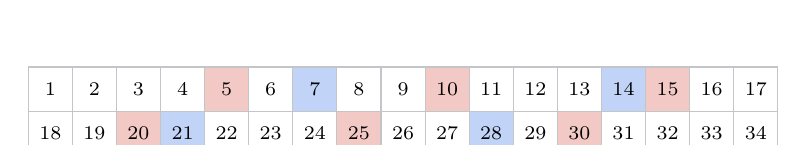
\begin{tikzpicture}[x=5.6mm,y=5.6mm]
  \foreach \k in {1,...,34}{
    \pgfmathtruncatemacro{\col}{mod(\k-1,17)}
    \pgfmathtruncatemacro{\row}{(\k-1)/17}
    \pgfmathtruncatemacro{\mf}{mod(\k,5)}
    \pgfmathtruncatemacro{\ms}{mod(\k,7)}
    \ifnum\mf=0 \fill[warn!30] (\col,-\row) rectangle ++(1,-1);\fi
    \ifnum\ms=0 \fill[acc!30] (\col,-\row) rectangle ++(1,-1);\fi
    \draw[gray!60] (\col,-\row) rectangle ++(1,-1);
    \node[font=\scriptsize] at (\col+0.5,-\row-0.5) {\k};
  }
\end{tikzpicture}\\[2pt]
{\footnotesize red = multiple of 5 (6 numbers), blue = multiple of 7 (4 numbers); $34 - 10 = 24$ white cells}
\end{center}

\begin{trap}[: repeated prime factors]
$25 = 5 \times 5$ is \textbf{not} a product of two distinct primes, so $(5-1)(5-1) = 16$ is wrong. Use rule 3: $\phi(25) = 25 - 5 = \mathbf{20}$. (Check: among $1, \dots, 24$ only 5, 10, 15, 20 share a factor with 25, leaving $24 - 4 = 20$.) The slides make the same point with $\phi(49)$: writing $\phi(49) = \phi(7)\phi(7) = 36$ is wrong because 7 and 7 are not co-prime; the correct value is $49 - 7 = 42$.
\end{trap}

\begin{worked}[: $\phi(n)$ from the factorisation (Forouzan / slide style)]
\textbf{Q.} Find (a) $\phi(29)$ (b) $\phi(32)$ (c) $\phi(80)$ (d) $\phi(100)$ (e) $\phi(101)$ (f) $\phi(240)$ (g) $\phi(1000)$ (h) $\phi(7000)$.

\textbf{A.} Factorise first, then apply the rules.
\begin{center}\small
\begin{tabular}{@{}llll@{}}
\toprule
$n$ & Factorisation & Working & $\phi(n)$\\
\midrule
29 & prime & $29 - 1$ & \textbf{28}\\
32 & $2^5$ & $2^5 - 2^4 = 32 - 16$ & \textbf{16}\\
80 & $2^4 \cdot 5$ & $(2^4 - 2^3)(5 - 1) = 8 \cdot 4$ & \textbf{32}\\
100 & $2^2 \cdot 5^2$ & $(4 - 2)(25 - 5) = 2 \cdot 20$ & \textbf{40}\\
101 & prime & $101 - 1$ & \textbf{100}\\
240 & $2^4 \cdot 3 \cdot 5$ & $(16 - 8)(3 - 1)(5 - 1) = 8 \cdot 2 \cdot 4$ & \textbf{64}\\
1000 & $2^3 \cdot 5^3$ & $1000 \cdot \frac12 \cdot \frac45$ \;(or $\phi(8)\phi(125) = 4 \cdot 100$) & \textbf{400}\\
7000 & $2^3 \cdot 5^3 \cdot 7$ & $7000 \cdot \frac12 \cdot \frac45 \cdot \frac67 = 7000 \cdot \frac{24}{70}$ & \textbf{2400}\\
\bottomrule
\end{tabular}
\end{center}
\textbf{Check:} a direct count of the co-prime $k < n$ by script gives the same eight values. Lecture homework: $\phi(369) = \phi(3^2)\phi(41) = 6 \cdot 40 = \mathbf{240}$ and $\phi(372) = \phi(2^2)\phi(3)\phi(31) = 2 \cdot 2 \cdot 30 = \mathbf{120}$.
\end{worked}

\textbf{$\phi(n)$ is even for every $n > 2$.} If $\gcd(k, n) = 1$ then also $\gcd(n - k, n) = 1$, so the co-prime numbers below $n$ come in pairs $\{k, n-k\}$. The two members of a pair can only coincide if $n = 2k$, but then $\gcd(k, n) = k$, which equals 1 only for $n = 2$. Hence for $n > 2$ the co-prime numbers split into disjoint pairs and their count is even; in $\mathbb{Z}_{14}^*$ the pairs are $\{1, 13\}$, $\{3, 11\}$, $\{5, 9\}$.

\subsection{The sets $\mathbb{Z}_n$ and $\mathbb{Z}_n^*$}
$\mathbb{Z}_n = \{0, 1, \dots, n-1\}$ is the set of residues modulo $n$. Every element has an additive inverse in it ($a + (n - a) \equiv 0$), but not every element has a multiplicative inverse. Since cryptosystems such as the affine cipher, Hill cipher and RSA need to \emph{divide}, they work in the smaller set
\[
\mathbb{Z}_n^* = \{\, a \in \mathbb{Z}_n : \gcd(a, n) = 1 \,\},
\]
which is exactly the set of residues that have multiplicative inverses. By definition its size is $|\mathbb{Z}_n^*| = \phi(n)$. The slide's rule of thumb: \imp{use $\mathbb{Z}_n$ when additive inverses are needed and $\mathbb{Z}_n^*$ when multiplicative inverses are needed.}

$\mathbb{Z}_n^*$ is closed under multiplication modulo $n$, because a product of two numbers co-prime to $n$ is again co-prime to $n$ (no prime factor of $n$ can appear in it). Together with the inverses this makes $\langle \mathbb{Z}_n^*, \times \rangle$ a group of order $\phi(n)$ (\S\ref{sec:algebra}), and the theorems of the next section are statements about this group. The slides single out the two sets with a \emph{prime} modulus, $\mathbb{Z}_p$ and $\mathbb{Z}_p^*$. When $n = p$ is prime, $\mathbb{Z}_p^* = \{1, 2, \dots, p-1\}$ contains every non-zero residue (e.g.\ $\mathbb{Z}_{13}^* = \{1, \dots, 12\}$), so every non-zero element of $\mathbb{Z}_p$ can be divided by, which is what makes $\mathbb{Z}_p$ the field GF$(p)$.
\begin{center}\small
\begin{tabular}{@{}lll@{}}
\toprule
$n$ & $\mathbb{Z}_n^*$ & $|\mathbb{Z}_n^*| = \phi(n)$\\
\midrule
6 & $\{1, 5\}$ & $\phi(2)\phi(3) = 2$\\
7 & $\{1, 2, 3, 4, 5, 6\}$ & $7 - 1 = 6$\\
10 & $\{1, 3, 7, 9\}$ & $\phi(2)\phi(5) = 4$\\
14 & $\{1, 3, 5, 9, 11, 13\}$ & $\phi(2)\phi(7) = 1 \cdot 6 = 6$ \;(slide Example 5)\\
21 & $\{1, 2, 4, 5, 8, 10, 11, 13, 16, 17, 19, 20\}$ & $\phi(3)\phi(7) = 2 \cdot 6 = 12$\\
26 & the 12 odd numbers except 13 & $\phi(2)\phi(13) = 12$ \;(valid keys/determinants mod 26)\\
\bottomrule
\end{tabular}
\end{center}

\subsection{Why cryptography cares about \texorpdfstring{$\phi(n)$}{phi(n)}}
Three later topics rest on $\phi(n)$. First, Euler's theorem (\S\ref{sec:fermat}) states that $a^{\phi(n)} \equiv 1 \pmod n$ for every $a \in \mathbb{Z}_n^*$, which allows exponents to be reduced modulo $\phi(n)$ and inverses to be computed as $a^{\phi(n)-1}$. Second, RSA chooses $n = pq$ and computes $\phi(n) = (p-1)(q-1)$; the keys satisfy $ed \equiv 1 \pmod{\phi(n)}$, and Euler's theorem then makes decryption undo encryption. In the standard example $n = 187 = 11 \cdot 17$, $\phi(187) = 160$ and $7 \cdot 23 = 161 \equiv 1 \pmod{160}$, which is why $88^7 \bmod 187 = 11$ and $11^{23} \bmod 187 = 88$ undo each other. Third, the number of primitive roots of a prime $p$ is $\phi(p - 1)$, which matters for Diffie--Hellman and ElGamal.

\textbf{Security.} Knowing $\phi(n)$ for an RSA modulus is equivalent to knowing its factors. From $n = pq$ and $\phi(n) = n - (p + q) + 1$ one gets $p + q = n - \phi(n) + 1$, and $p, q$ are then the roots of $z^2 - (p+q)z + n = 0$. For $n = 143$ and $\phi(n) = 120$: $p + q = 24$, $pq = 143$, so $p, q = \mathbf{11, 13}$. This is why $\phi(n)$ is part of the private key.

\begin{fixbox}
\begin{itemize}
  \item All values recomputed by script: $\phi(5) = 4$, $\phi(8) = 4$, $\phi(11) = 10$, $\phi(35) = 24$, $\phi(25) = 20$, $\phi(49) = 42$, $\phi(240) = 64$, $\phi(1000) = 400$, $\phi(7000) = 2400$, $|\mathbb{Z}_{14}^*| = 6$, $|\mathbb{Z}_{21}^*| = 12$. The homework answers in the old notes ($\phi(369) = 240$, $\phi(372) = 120$) are correct.
  \item Slide L10-06 gives $\phi(1) = 0$, which follows Forouzan's ``integers smaller than $n$'' wording. The standard convention is $\phi(1) = 1$ (count $1 \le k \le n$). It only affects $n = 1$ and never matters in RSA.
  \item The lecture video's ``case 3'' (``either or both numbers composite'') makes the product formula $n\prod(1 - 1/p)$ look like a last resort. It actually works for every $n$, and the prime and $pq$ formulas are special cases of it.
\end{itemize}
\end{fixbox}

% Lecture 10 (Fermat, Euler, inverses), Lecture 11 (order, primitive roots) + videos. All numbers recomputed by script (scratchpad/euler/v11.py).
\section{Fermat's and Euler's Theorems, Inverses and Primitive Roots}\label{sec:fermat}

Public-key cryptography computes powers $a^b \bmod n$ with exponents hundreds of digits long, and it needs inverses modulo $n$. Square-and-multiply (\S\ref{sec:modexp}) makes such powers feasible, but the two theorems of this section do more: they say that the powers of $a$ modulo $n$ repeat with a known period, so a huge exponent can be replaced by a small one, and they give a formula for the inverse. The same periodicity, studied element by element, leads to the order of an element and to primitive roots, which Diffie--Hellman and ElGamal are built on.

\subsection{Fermat's little theorem and exponent reduction \hot}
\asked{Mid-sem 2024--25 Q5(ii) (part of 3 marks): $100^{95} \bmod 9$, $658^{17} \bmod 17$, $145^{102} \bmod 101$.}
\textbf{First version.} \imp{If $p$ is prime and $a$ is an integer not divisible by $p$, then $a^{p-1} \equiv 1 \pmod p$.} Both conditions must be checked before the theorem is used: for a composite modulus or for $p \mid a$ it says nothing.

\textbf{Why it is true.} Multiply each of $1, 2, \dots, p-1$ by $a$ and reduce modulo $p$. No product is 0, because $p$ divides neither factor, and no two products are equal, because $ai \equiv aj$ would mean $p \mid a(i - j)$ and hence $p \mid (i - j)$, i.e.\ $i = j$. The $p - 1$ products are therefore just $1, \dots, p-1$ in a different order; for $p = 7$, $a = 3$ they are $3, 6, 2, 5, 1, 4$. Multiplying all of them together gives $a^{p-1}(p-1)! \equiv (p-1)! \pmod p$, and since $(p-1)!$ is co-prime to $p$ it can be cancelled, leaving $a^{p-1} \equiv 1$.

\textbf{Second version.} \imp{If $p$ is prime, then $a^p \equiv a \pmod p$ for every integer $a$.} This removes the condition on $a$. If $p \nmid a$, it is the first version multiplied by $a$; if $p \mid a$, both sides are $\equiv 0$.
\begin{center}\small
\begin{tabular}{@{}llll@{}}
\toprule
$p$, $a$ & Conditions & Working & Result\\
\midrule
5, 2 & prime, $5 \nmid 2$ & $2^4 = 16 = 3\cdot5 + 1$ & $\equiv 1$ \checkmark\\
13, 11 & prime, $13 \nmid 11$ & $11 \equiv -2$, $(-2)^{12} = \big((-2)^4\big)^3 = 16^3 \equiv 3^3 = 27 \equiv 1$ & $\equiv 1$ \checkmark\\
6, 2 & \textbf{6 not prime} & $2^5 = 32 = 5\cdot6 + 2$ & $\equiv 2 \ne 1$: theorem silent\\
11, 5 (homework) & prime, $11 \nmid 5$ & $5^2 \equiv 3$, $5^4 \equiv 9$, $5^8 \equiv 81 \equiv 4$, $5^{10} = 5^8 \cdot 5^2 \equiv 4 \cdot 3 = 12$ & $\equiv 1$ \checkmark\\
\bottomrule
\end{tabular}
\end{center}

\textbf{Exponent reduction.} Since $a^{p-1} \equiv 1$, the powers of $a$ modulo $p$ repeat with period dividing $p - 1$. Writing the exponent as $b = q(p-1) + r$ with $r = b \bmod (p-1)$ gives
\[
a^b = \left(a^{p-1}\right)^q a^r \equiv 1^q \cdot a^r = a^{\,b \bmod (p-1)} \pmod p \qquad (p \text{ prime},\ p \nmid a).
\]
The slides' examples follow directly: $6^{10} \bmod 11 = 1$ because the exponent is exactly $p - 1$, and $3^{12} \bmod 11 = 3^{11} \cdot 3 \equiv 3 \cdot 3 = 9$ by the second version (equivalently $12 \bmod 10 = 2$ and $3^2 = 9$). In practice the base is reduced modulo $p$ first, then the exponent modulo $p - 1$, and the small power that remains is computed by repeated squaring.

\begin{trap}[: what to reduce, and by what]
The \textbf{base} is reduced modulo $p$; the \textbf{exponent} is reduced modulo $p - 1$, never modulo $p$. And the modulus must be prime: in $100^{95} \bmod 9$ the modulus $9 = 3^2$ is composite, so Fermat does not apply. There the base reduction alone finishes the job ($100 \equiv 1 \pmod 9$), or Euler's theorem with $\phi(9) = 6$ can be used.
\end{trap}

\begin{worked}[: exponent reduction by Fermat (Forouzan exercise)]
\textbf{Q.} Using Fermat's little theorem, find (a) $5^{15} \bmod 13$ (b) $15^{18} \bmod 17$ (c) $456^{17} \bmod 17$.

\textbf{A.}
\begin{center}\small
\begin{tabular}{@{}lllll@{}}
\toprule
 & Conditions & Base & Exponent & Result\\
\midrule
(a) & 13 prime, $13 \nmid 5$ & 5 & $15 = 1\cdot12 + 3 \to 3$ & $5^3 = 125 = 9\cdot13 + 8 \Rightarrow \mathbf{8}$\\
(b) & 17 prime, $17 \nmid 15$ & $15 \equiv -2$ & $18 = 1\cdot16 + 2 \to 2$ & $(-2)^2 = \mathbf{4}$\\
(c) & 17 prime & $456 = 26\cdot17 + 14 \to 14$ & second version: $a^{17} \equiv a$ & $\mathbf{14}$\\
\bottomrule
\end{tabular}
\end{center}
\textbf{Check} (by script): $5^{15} \bmod 13 = 8$, $15^{18} \bmod 17 = 4$, $456^{17} \bmod 17 = 14$.
\end{worked}

\textbf{Fermat as a primality test.} Read backwards, the theorem gives a test: if $a^{n-1} \not\equiv 1 \pmod n$ for some $a$ with $\gcd(a, n) = 1$, then $n$ is certainly composite (e.g.\ $2^{14} \bmod 15 = 4$). The converse fails: $2^{340} \equiv 1 \pmod{341}$ although $341 = 11 \cdot 31$. The Fermat test, Carmichael numbers and Miller--Rabin are covered in \S\ref{sec:primes}.

\subsection{Euler's theorem \hot}
\asked{End-sem 2025--26 Q6(b): short note on Euler's theorem (2 marks).}
\likely{Exponent reduction modulo $\phi(n)$ for a composite $n$, and ``why does RSA decryption work?'' (Euler is its basis).}
Fermat's theorem needs a prime modulus, but RSA works modulo $n = pq$. Euler's theorem is the generalisation to any modulus. \textbf{First version:} \imp{if $\gcd(a, n) = 1$, then $a^{\phi(n)} \equiv 1 \pmod n$.} When $n = p$ is prime, $\phi(p) = p - 1$ and this is exactly Fermat's theorem.

\textbf{Why it is true.} The proof is the same permutation argument, run over $\mathbb{Z}_n^*$ (\S\ref{sec:totient}) instead of $\{1, \dots, p-1\}$. Multiplying the $\phi(n)$ elements of $\mathbb{Z}_n^*$ by $a$ permutes them, because $a$ is invertible; for $n = 10$, $a = 3$ the set $\{1, 3, 7, 9\}$ becomes $\{3, 9, 1, 7\}$. Taking the product of all elements on both sides gives $a^{\phi(n)} \cdot \Pi \equiv \Pi$, and the product $\Pi$ is invertible, so $a^{\phi(n)} \equiv 1$.

The co-prime condition is genuinely needed. If $\gcd(a, n) = d > 1$, every power of $a$ is a multiple of $d$, and so is every number $\equiv a^k \pmod n$; such a number can never be $\equiv 1$. The lecture homework $11^{20} \bmod 33$ shows this: the powers of 11 alternate $11, 22, 11, 22, \dots$, so $11^{20} \equiv 22 \ne 1$ although $\phi(33) = 20$.
\begin{center}\small
\begin{tabular}{@{}llll@{}}
\toprule
$a$, $n$ & $\gcd$ & Working & Result\\
\midrule
3, 10 & 1 & $\phi(10) = 4$; $3^4 = 81 = 8\cdot10 + 1$ & $\equiv 1$ \checkmark\\
2, 10 & \textbf{2} & $2^4 = 16 \equiv 6$ & $\ne 1$: theorem silent\\
10, 11 & 1 & $\phi(11) = 10$; $10 \equiv -1$, $(-1)^{10} = 1$ & $\equiv 1$ \checkmark\\
6, 35 & 1 & $\phi(35) = 24$; slide example $6^{24} \bmod 35$ & $\equiv 1$ \checkmark\\
11, 33 (homework) & \textbf{11} & $\phi(33) = 20$; powers alternate $11, 22$ & $11^{20} \equiv 22 \ne 1$\\
\bottomrule
\end{tabular}
\end{center}

\textbf{Exponent reduction.} Exactly as with Fermat, $\gcd(a, n) = 1$ and $b = q\phi(n) + r$ give $a^b \equiv a^{\,b \bmod \phi(n)} \pmod n$. The work is in computing $\phi(n)$, which needs the factorisation of $n$.

\textbf{Second version.} \imp{For $n = pq$ (and more generally any squarefree $n$), $a^{k\phi(n)+1} \equiv a \pmod n$ for every integer $a$ and every $k \ge 0$.} This removes the co-prime condition, which RSA needs because a message $M$ might, by bad luck, share the factor $p$ with $n$. The proof works one prime at a time. Modulo $p$: if $p \nmid a$, then $a^{k\phi(n)} = \big(a^{p-1}\big)^{k(q-1)} \equiv 1$ by Fermat, so $a^{k\phi(n)+1} \equiv a$; if $p \mid a$, both sides are $\equiv 0$. The same holds modulo $q$. Since the distinct primes $p$ and $q$ both divide $a^{k\phi(n)+1} - a$, so does $pq$. For example $11^{21} = 11^{\phi(33)+1} \equiv 11 \pmod{33}$ although $\gcd(11, 33) \ne 1$. The argument breaks when a prime appears squared: for $n = 4$, $a = 2$, $k = 1$ the claim would be $2^3 \equiv 2$, but $2^3 = 8 \equiv 0 \pmod 4$.

\textbf{Why RSA decryption works.} RSA picks $e$ and $d$ with $ed \equiv 1 \pmod{\phi(n)}$, i.e.\ $ed = k\phi(n) + 1$. Decrypting $C = M^e$ gives $C^d = M^{ed} = M^{k\phi(n)+1} \equiv M \pmod n$ by the second version, for every message $M < n$. In the example $n = 187$, $e = 7$, $d = 23$: $ed = 161 = 1 \cdot 160 + 1$, and indeed $88^7 \bmod 187 = 11$ and $11^{23} \bmod 187 = 88$.

\begin{mustknow}
\begin{center}\small
\begin{tabular}{@{}lll@{}}
\toprule
 & First version & Second version (no co-prime condition)\\
\midrule
Fermat ($p$ prime) & $a^{p-1} \equiv 1 \pmod p$ if $p \nmid a$ & $a^p \equiv a \pmod p$\\
Euler & $a^{\phi(n)} \equiv 1 \pmod n$ if $\gcd(a,n) = 1$ & $a^{k\phi(n)+1} \equiv a \pmod n$ ($n = pq$, squarefree)\\
\midrule
Reduction & \multicolumn{2}{l}{$a^b \equiv a^{\,b \bmod (p-1)} \pmod p$ \quad and \quad $a^b \equiv a^{\,b \bmod \phi(n)} \pmod n$ \quad (co-prime $a$)}\\
Inverse & \multicolumn{2}{l}{$a^{-1} \equiv a^{p-2} \pmod p$ \quad and \quad $a^{-1} \equiv a^{\phi(n)-1} \pmod n$ \quad (co-prime $a$)}\\
\bottomrule
\end{tabular}
\end{center}
\end{mustknow}

\begin{worked}[: exponent reduction by Euler]
\textbf{Q.} Using Euler's theorem, find (a) $11^{2024} \bmod 35$ (b) the last two digits of $3^{1003}$ (c) $20^{62} \bmod 77$ (slide example).

\textbf{A.}
\begin{center}\small
\begin{tabular}{@{}lllll@{}}
\toprule
 & $\gcd$, $\phi(n)$ & Exponent & Remaining power & Result\\
\midrule
(a) & $\gcd(11, 35) = 1$, $\phi(35) = 4 \cdot 6 = 24$ & $2024 = 84\cdot24 + 8$ & $11^2 = 121 \equiv 16$, $11^4 \equiv 16^2 = 256 \equiv 11$, $11^8 \equiv 11^2 \equiv 16$ & $\mathbf{16}$\\
(b) & $\gcd(3, 100) = 1$, $\phi(100) = 40$ & $1003 = 25\cdot40 + 3$ & $3^3 = 27$ & $\mathbf{27}$\\
(c) & $\gcd(20, 77) = 1$, $\phi(77) = 6 \cdot 10 = 60$ & $62 = 1\cdot60 + 2$ & $20^2 = 400 = 5\cdot77 + 15$ & $\mathbf{15}$\\
\bottomrule
\end{tabular}
\end{center}
For (b), ``last two digits'' means the residue modulo 100. \textbf{Check} (by script): $11^{2024} \bmod 35 = 16$, $3^{1003} \bmod 100 = 27$, $20^{62} \bmod 77 = 15$.
\end{worked}

\subsection{Multiplicative inverses via Fermat and Euler \hot}
\asked{Mid-sem 2024--25 Q5(iii): $7^{-1} \bmod 17$, $15^{-1} \bmod 99$ (does not exist).}
The multiplicative inverse of $a$ modulo $n$ is the residue $a^{-1}$ with \imp{$a \cdot a^{-1} \equiv 1 \pmod n$; it exists if and only if $\gcd(a, n) = 1$} (derived in \S\ref{sec:totient}). It depends on the modulus as well as on $a$: $2^{-1}$ is 3 modulo 5 but 4 modulo 7. For small $n$ it can be found by trial, multiplying $a$ by $1, 2, 3, \dots$ until the product is $\equiv 1$:
\begin{center}\small
\begin{tabular}{@{}lllll@{}}
\toprule
$a \bmod n$ & $\gcd$ & Search & Inverse & Note\\
\midrule
$3 \bmod 5$ & 1 & $3\cdot2 = 6 \equiv 1$ & \textbf{2} & so $2^{-1} \bmod 5 = 3$ as well\\
$2 \bmod 11$ & 1 & $2\cdot6 = 12 \equiv 1$ & \textbf{6} & \\
$4 \bmod 5$ & 1 & $4\cdot4 = 16 \equiv 1$ & \textbf{4} & its own inverse ($4 \equiv -1$)\\
$2 \bmod 7$ & 1 & $2\cdot4 = 8 \equiv 1$ & \textbf{4} & not 3: depends on $n$\\
$5 \bmod 10$ & \textbf{5} & $5k \bmod 10 \in \{0, 5\}$ only & \textbf{none} & \\
\bottomrule
\end{tabular}
\end{center}

\textbf{Inverse by exponentiation.} Fermat's theorem already contains the inverse. If $p$ is prime and $p \nmid a$, then $a \cdot a^{p-2} = a^{p-1} \equiv 1$, so
\[
a^{-1} \equiv a^{p-2} \pmod p, \qquad\text{and in the same way}\qquad a^{-1} \equiv a^{\phi(n)-1} \pmod n \ \text{ if } \gcd(a, n) = 1.
\]
This replaces the extended Euclidean algorithm by one modular exponentiation, which is convenient when the modulus is prime or when $\phi(n)$ is known. The price is that for a composite $n$ the factorisation is needed to get $\phi(n)$. The slides' examples (L10-15 and L10-20), all checked by script:
\begin{center}\small
\begin{tabular}{@{}ll@{\qquad}lll@{}}
\toprule
\multicolumn{2}{@{}l}{Fermat ($n$ prime)} & \multicolumn{3}{l}{Euler ($n$ composite)}\\
\midrule
$8^{-1} \bmod 17 = 8^{15}$ & $= 15$ & $8^{-1} \bmod 77 = 8^{59}$ & $= 29$ & $\phi(77) = 60$\\
$5^{-1} \bmod 23 = 5^{21}$ & $= 14$ & $7^{-1} \bmod 15 = 7^{7}$ & $= 13$ & $\phi(15) = 8$\\
$60^{-1} \bmod 101 = 60^{99}$ & $= 32$ & $60^{-1} \bmod 187 = 60^{159}$ & $= 53$ & $\phi(187) = 160$\\
$22^{-1} \bmod 211 = 22^{209}$ & $= 48$ & $71^{-1} \bmod 100 = 71^{39}$ & $= 31$ & $\phi(100) = 40$\\
$2^{-1} \bmod 13 = 2^{11}$ & $= 7$ & $3^{-1} \bmod 20 = 3^{7}$ & $= 7$ & $\phi(20) = 8$\\
\bottomrule
\end{tabular}
\end{center}
Each answer is checked by one multiplication, e.g.\ $8 \cdot 15 = 120 = 7\cdot17 + 1$ and $7 \cdot 13 = 91 = 6\cdot15 + 1$.

\begin{trap}[: the inverse may not exist]
Before using any formula, compute $\gcd(a, n)$. If it is not 1 there is no inverse, and the exam expects exactly that answer with the reason. Blindly applying Euler's formula still produces a number, which is wrong: for $15^{-1} \bmod 99$, $\phi(99) = 60$ and $15^{59} \bmod 99 = 36$, but $15 \cdot 36 = 540 \equiv 45 \not\equiv 1 \pmod{99}$.
\end{trap}

\begin{worked}[: 2024--25 Q5(ii) and (iii), as it should be written]
\textbf{Q.} (ii) Find the values of $100^{95} \bmod 9$, $658^{17} \bmod 17$ and $145^{102} \bmod 101$. (iii) Find the values of $7^{-1} \bmod 17$ and $15^{-1} \bmod 99$.

\textbf{A.} (ii) \textbf{$100^{95} \bmod 9$.} The modulus 9 is not prime, so Fermat's theorem cannot be used; reduce the base instead. $100 = 11 \cdot 9 + 1$, so $100 \equiv 1 \pmod 9$ and $100^{95} \equiv 1^{95} = \mathbf{1}$. (Euler agrees: $\gcd(100, 9) = 1$, $\phi(9) = 6$, $95 \bmod 6 = 5$, $1^5 = 1$.)

\textbf{$658^{17} \bmod 17$.} 17 is prime, so by the second version of Fermat's theorem $a^{17} \equiv a \pmod{17}$. $658 = 38 \cdot 17 + 12$, hence $658^{17} \equiv 658 \equiv \mathbf{12}$.

\textbf{$145^{102} \bmod 101$.} 101 is prime and $101 \nmid 145$. Base: $145 \equiv 44$. Exponent: $102 = 1 \cdot 100 + 2$, and $44^{100} \equiv 1$ by Fermat. So $145^{102} \equiv 44^2 = 1936 = 19 \cdot 101 + 17$, i.e.\ $\mathbf{17}$.

(iii) \textbf{$7^{-1} \bmod 17$.} 17 is prime and $17 \nmid 7$, so $7^{-1} \equiv 7^{17-2} = 7^{15} \pmod{17}$. With $15 = 8 + 4 + 2 + 1$:
\begin{center}\small
\begin{tabular}{@{}lllll@{}}
\toprule
$7^1$ & $7^2$ & $7^4$ & $7^8$ & $7^{15} = 7^8 \cdot 7^4 \cdot 7^2 \cdot 7$\\
\midrule
7 & $49 \equiv 15$ & $15^2 = 225 \equiv 4$ & $4^2 = 16$ & $16 \cdot 4 = 64 \equiv 13$;\; $13 \cdot 15 = 195 \equiv 8$;\; $8 \cdot 7 = 56 \equiv \mathbf{5}$\\
\bottomrule
\end{tabular}
\end{center}
So $7^{-1} \bmod 17 = \mathbf{5}$. Check: $7 \cdot 5 = 35 = 2 \cdot 17 + 1$ \checkmark.

\textbf{$15^{-1} \bmod 99$.} $\gcd(99, 15)$: $99 = 6 \cdot 15 + 9$, $15 = 1 \cdot 9 + 6$, $9 = 1 \cdot 6 + 3$, $6 = 2 \cdot 3 + 0$, so $\gcd = 3 \ne 1$. Every number $15x - 99k$ is a multiple of 3 and can never equal 1, therefore \textbf{$15^{-1} \bmod 99$ does not exist}.
\end{worked}

\textbf{Which method?} All four methods give the same inverse when it exists; they differ in what they need. The summary below is the decision to make in an exam.
\begin{center}\small
\begin{tabularx}{\textwidth}{@{}l l X@{}}
\toprule
Method & Formula & When to use\\
\midrule
Trial & $a\cdot1, a\cdot2, \dots$ until $\equiv 1$ & Small $n$ only (mod 26 ciphers, GF(7) division).\\
Fermat & $a^{-1} = a^{p-2} \bmod p$ & Prime modulus; compute with square-and-multiply.\\
Euler & $a^{-1} = a^{\phi(n)-1} \bmod n$ & Composite $n$ whose factorisation (hence $\phi(n)$) is known.\\
\textbf{Extended Euclid} & $sa + tn = 1 \Rightarrow a^{-1} = s \bmod n$ & The general method: works for any $n$ without factoring, and detects ``no inverse'' (final $\gcd \ne 1$). The past papers ask for it explicitly (2024--25 Q7, \S\ref{sec:exteuclid}); RSA uses it to find $d$.\\
\bottomrule
\end{tabularx}
\end{center}

\subsection{Order of an element \new}
\likely{``Find the order of every element of $\mathbb{Z}_7^*$ / $\mathbb{Z}_{10}^*$'' (Forouzan), usually as the first step of a primitive-root question.}
Euler's theorem says that $a^{\phi(n)} \equiv 1$ for every $a \in \mathbb{Z}_n^*$, but many elements return to 1 much earlier. \imp{The order of $a$ modulo $n$, $\operatorname{ord}(a)$, is the smallest positive integer $i$ with $a^i \equiv 1 \pmod n$.} It exists for every $a \in \mathbb{Z}_n^*$, and Euler's theorem guarantees $\operatorname{ord}(a) \le \phi(n)$. After $a^{\operatorname{ord}(a)} = 1$ the powers start over, so the sequence $a, a^2, a^3, \dots$ is periodic with period exactly $\operatorname{ord}(a)$.

\textbf{The key property: $a^m \equiv 1 \iff \operatorname{ord}(a) \mid m$.} Write $m = q \cdot \operatorname{ord}(a) + r$ with $0 \le r < \operatorname{ord}(a)$. Then $a^m = \big(a^{\operatorname{ord}(a)}\big)^q a^r \equiv a^r$, and by the minimality of the order $a^r \equiv 1$ only for $r = 0$. Two consequences follow. First, since $a^{\phi(n)} \equiv 1$, \textbf{the order always divides $\phi(n)$} (this is Lagrange's theorem for the group $\mathbb{Z}_n^*$), so to find an order only the divisors of $\phi(n)$ need to be tried. Second, exponents can be reduced modulo $\operatorname{ord}(a)$, which is sharper than reducing modulo $\phi(n)$: $\operatorname{ord}(2) = 3$ modulo 7, so $2^{100} \equiv 2^{100 \bmod 3} = 2^1 = 2 \pmod 7$.

The table lists $a^i \bmod 7$ for the whole group $\mathbb{Z}_7^*$ (slide L11-30); the shaded cell is the first 1 in each row, and its column is the order. Every order is a divisor of $\phi(7) = 6$, and only $a = 3$ and $a = 5$ reach the maximum 6.
\begin{center}\small
\begin{tabular}{@{}c|cccccc|c@{}}
\toprule
$a$ & $i=1$ & 2 & 3 & 4 & 5 & 6 & $\operatorname{ord}(a)$\\
\midrule
1 & \hl{1} & 1 & 1 & 1 & 1 & 1 & 1\\
2 & 2 & 4 & \hl{1} & 2 & 4 & 1 & 3\\
3 & 3 & 2 & 6 & 4 & 5 & \hl{1} & \textbf{6}\\
4 & 4 & 2 & \hl{1} & 4 & 2 & 1 & 3\\
5 & 5 & 4 & 6 & 2 & 3 & \hl{1} & \textbf{6}\\
6 & 6 & \hl{1} & 6 & 1 & 6 & 1 & 2\\
\bottomrule
\end{tabular}
\end{center}
Two more slide examples (L11-27, L11-29): in $\mathbb{Z}_{10}^* = \{1, 3, 7, 9\}$ the orders are $1, 4, 4, 2$ ($3^2 = 9$, $3^4 = 81 \equiv 1$), and in $\mathbb{Z}_8^* = \{1, 3, 5, 7\}$ they are $1, 2, 2, 2$, because $3^2 = 9$, $5^2 = 25$ and $7^2 = 49$ are all $\equiv 1 \pmod 8$.

\subsection{Primitive roots \hot}
\asked{End-sem 2025--26 Q2(a)(i): find the primitive roots of GF(19) (they are 2, 3, 10, 13, 14, 15).}
\likely{``Find all primitive roots of 7 / 11 / 13'', ``is 3 a primitive root of 17?'', ``how many primitive roots does 17 have?'' (needed for Diffie--Hellman and ElGamal).}

\textbf{The idea, for a prime $p$.} Take the multiplicative group $\mathbb{Z}_p^* = \{1, 2, \dots, p-1\}$, which is $\mathbb{Z}_p$ without 0. Pick an element $g$ and write down its powers $g^1, g^2, g^3, \dots \pmod p$. Two things can happen. Either the powers run through \emph{every} element of $\mathbb{Z}_p^*$ before returning to 1, or they hit 1 early and then repeat a smaller cycle. In the first case \imp{$g$ is called a primitive root of $p$: its powers $g^1, \dots, g^{p-1}$ produce each of $1, \dots, p-1$ exactly once.} Modulo 7, for example:
\begin{center}\small
\begin{tabular}{@{}lccccccl@{}}
\toprule
 & $g^1$ & $g^2$ & $g^3$ & $g^4$ & $g^5$ & $g^6$ & \\
\midrule
$g = 3$ & 3 & 2 & 6 & 4 & 5 & 1 & all six elements: \textbf{primitive root}\\
$g = 2$ & 2 & 4 & 1 & 2 & 4 & 1 & only $\{2, 4, 1\}$: \textbf{not} a primitive root\\
\bottomrule
\end{tabular}
\end{center}
Since the powers start repeating as soon as they reach 1, the number of different powers equals the order of $g$. Producing all $p - 1$ elements therefore means exactly that \textbf{$\operatorname{ord}(g) = p - 1$}, the largest order possible. When such a $g$ exists, every element of the group is a power of it, so the group is \emph{cyclic} and $g$ is a \emph{generator}. Every element $y$ is then $g^x$ for exactly one $x \in \{1, \dots, p-1\}$, and that $x$ is the discrete logarithm of $y$ (\S\ref{sec:primes}).

\textbf{Why cryptography needs them.} Diffie--Hellman and ElGamal publish $p$ and a base $g$, keep an exponent $x$ secret, and publish $g^x \bmod p$. If $g$ had a small order $d$, then $g^x$ could take only $d$ different values, and Eve could find a matching exponent by trying $d$ values. Choosing a primitive root makes all $p - 1$ values possible, so the search is as large as it can be.

\textbf{The same idea for any $n$.} Nothing changes except the group. For a general $n$ the group is $\mathbb{Z}_n^*$, the numbers below $n$ that are coprime to $n$, and it has $\phi(n)$ elements instead of $p - 1$. So \imp{$g \in \mathbb{Z}_n^*$ is a primitive root of $n$ if $\operatorname{ord}(g) = \phi(n)$}, which means $g^1, \dots, g^{\phi(n)}$ produce every element of $\mathbb{Z}_n^*$ once each. Modulo 10, $\mathbb{Z}_{10}^* = \{1, 3, 7, 9\}$ and the powers of 3 are $3, 9, 7, 1$, so 3 is a primitive root of 10. The powers never produce 0, 2, 4, 5, 6 or 8, and they are not supposed to: a power of a number coprime to $n$ is itself coprime to $n$, so only $\mathbb{Z}_n^*$ can ever be generated, never all of $\mathbb{Z}_n$. For a prime this is the same statement as before, since $\mathbb{Z}_p^*$ is $\mathbb{Z}_p$ without 0 and $\phi(p) = p - 1$.

Unlike primes, many composite $n$ have \emph{no} primitive root at all, because every element returns to 1 too early. Modulo 8, the group $\mathbb{Z}_8^* = \{1, 3, 5, 7\}$ has $\phi(8) = 4$ elements, but $3^2$, $5^2$ and $7^2$ are all $\equiv 1$, so no order reaches 4 (slide L11-28). Modulo 15, every element satisfies $a^4 \equiv 1$, because $a^2 \equiv 1 \pmod 3$ and $a^4 \equiv 1 \pmod 5$, so no order reaches $\phi(15) = 8$. The complete answer is a theorem worth memorising:

\begin{mustknow}[: primitive roots]
$g$ is a primitive root of $n$ $\iff$ $\operatorname{ord}(g) = \phi(n)$ $\iff$ the powers of $g$ produce all of $\mathbb{Z}_n^*$ (for a prime: all of $1, \dots, p-1$).\\
Primitive roots exist \textbf{only} for $n = 2,\ 4,\ p^k,\ 2p^k$ ($p$ an odd prime). Every prime has them; 9, 10, 18 have them; 8, 12, 15 do not.\\
When they exist there are exactly $\phi(\phi(n))$ of them; for a prime $p$ that is $\phi(p-1)$.
\end{mustknow}

\textbf{Test 1: list the powers.} Multiply by $g$ repeatedly, reducing each time; for example $3^4 \equiv 6 \cdot 3 = 18 \equiv 4 \pmod 7$, so you never need $3^6 = 729$. If a 1 appears before the $(p-1)$-th power, stop: $g$ is not a primitive root.
\begin{center}\small
\begin{tabular}{@{}lll@{}}
\toprule
Test & Powers $g^1, g^2, \dots \pmod p$ & Verdict\\
\midrule
2 mod 5 & 2, 4, 3, 1 & order 4 $= p - 1$: \textbf{yes}\\
3 mod 5 & 3, 4, 2, 1 & \textbf{yes}\\
4 mod 5 & 4, \textbf{1} & order 2: no\\
3 mod 7 & 3, 2, 6, 4, 5, 1 & \textbf{yes}\\
2 mod 7 & 2, 4, \textbf{1} & order 3: no\\
2 mod 11 (homework) & 2, 4, 8, 5, 10, 9, 7, 3, 6, 1 & \textbf{yes}\\
\bottomrule
\end{tabular}
\end{center}
The homework ``primitive roots of 5'' is answered by the first three rows: 1 never works ($1^k = 1$), 2 and 3 do, and 4 does not, so the primitive roots of 5 are \textbf{2 and 3}.

\textbf{Test 2: the fast test.} Listing takes up to $p - 1$ multiplications. It is faster to use the fact that the order of $g$ must divide $p - 1$: if $g$ is not a primitive root, its order is a proper divisor of $p - 1$, and every proper divisor divides $(p-1)/q$ for some prime factor $q$ of $p - 1$. So it is enough to check those few exponents:
\begin{center}
\imp{$g$ is a primitive root of $p$ $\iff$ $g^{(p-1)/q} \not\equiv 1 \pmod p$ for every prime $q$ dividing $p - 1$.}
\end{center}
For $p = 7$, $p - 1 = 6 = 2 \cdot 3$, so check $g^3$ and $g^2$. For $g = 3$: $3^3 = 27 \equiv 6$ and $3^2 = 9 \equiv 2$, neither is 1, so 3 is a primitive root. For $g = 2$: $2^3 = 8 \equiv 1$, so 2 is not.

\textbf{Finding all of them from one.} Once one primitive root $g$ is known, the others are the powers $g^k$ with $\gcd(k, p-1) = 1$. The reason is that $g^k$ has order $\frac{p-1}{\gcd(k,\,p-1)}$, which equals $p - 1$ exactly when the gcd is 1. Counting those $k$ gives the $\phi(p-1)$ from the box: 5 has $\phi(4) = 2$ (2, 3), 7 has $\phi(6) = 2$ (3, 5), 11 has $\phi(10) = 4$ (2, 6, 7, 8), and 13 has $\phi(12) = 4$ (2, 6, 7, 11).

\begin{worked}[: all primitive roots of a prime]
\textbf{Q.} Find all the primitive roots of 11 (i.e.\ of the group $G = \langle \mathbb{Z}_{11}^*, \times \rangle$).

\textbf{A.} $\phi(11) = 10 = 2 \cdot 5$, so a primitive root $g$ must satisfy $g^{10/2} = g^5 \not\equiv 1$ and $g^{10/5} = g^2 \not\equiv 1$. Try $g = 2$: $2^2 = 4 \ne 1$ and $2^5 = 32 = 2\cdot11 + 10 \equiv 10 \ne 1$, so \textbf{2 is a primitive root}. (For contrast, $g = 3$ fails: $3^5 = 243 = 22 \cdot 11 + 1 \equiv 1$.)

The other primitive roots are $2^k$ with $\gcd(k, 10) = 1$, i.e.\ $k \in \{1, 3, 7, 9\}$:
\begin{center}\small
\begin{tabular}{@{}lcccc@{}}
\toprule
$k$ & 1 & 3 & 7 & 9\\
$2^k \bmod 11$ & 2 & 8 & $128 = 11\cdot11 + 7 \to 7$ & $512 = 46\cdot11 + 6 \to 6$\\
\bottomrule
\end{tabular}
\end{center}
The primitive roots of 11 are \textbf{2, 6, 7, 8}. \textbf{Check:} their number is $\phi(10) = 4$ \checkmark, and the full list of powers of 2 is $2, 4, 8, 5, 10, 9, 7, 3, 6, 1$, all ten residues.
\end{worked}

\begin{worked}[: fast test and counting]
\textbf{Q.} Show that 3 is a primitive root of 17 but 2 is not. How many primitive roots does 17 have? List them.

\textbf{A.} $\phi(17) = 16 = 2^4$, whose only prime factor is 2, so $g$ is a primitive root iff $g^{16/2} = g^8 \not\equiv 1 \pmod{17}$.
For $g = 3$: $3^2 = 9$, $3^4 = 81 \equiv 13$, $3^8 \equiv 13^2 = 169 \equiv 16 \ne 1$, so \textbf{3 is a primitive root}.
For $g = 2$: $2^4 = 16$, $2^8 \equiv 16^2 = 256 = 15\cdot17 + 1 \equiv 1$, so \textbf{2 is not} (its order is 8).
The number of primitive roots is $\phi(16) = \mathbf{8}$. They are $3^k$ for odd $k$: $3^1, 3^3, \dots, 3^{15} \equiv 3, 10, 5, 11, 14, 7, 12, 6$, i.e.\ \textbf{3, 5, 6, 7, 10, 11, 12, 14}.
\end{worked}

\begin{fixbox}
\begin{itemize}
  \item All values recomputed by script. The slides' inverse examples (L10-15: 15, 14, 32, 48; L10-20: 29, 13, 53, 31) and examples $6^{10} \bmod 11 = 1$, $3^{12} \bmod 11 = 9$, $6^{24} \bmod 35 = 1$, $20^{62} \bmod 77 = 15$ are correct. The video homework answers are correct: $5^{10} \equiv 1 \pmod{11}$, $11^{20} \equiv 22 \pmod{33}$, 2 is a primitive root of 11, the primitive roots of 5 are 2 and 3.
  \item Slide L10-16 says the second version of Euler's theorem ``removes the condition that $a$ and $n$ should be coprime''. That is true only for squarefree $n$ (such as $n = pq$ in RSA). It fails for $n = 4$, $a = 2$: $2^{\phi(4)+1} = 2^3 = 8 \equiv 0 \not\equiv 2$.
  \item Slide L10-18 solves $20^{62} \bmod 77$ with the second version, but $\gcd(20, 77) = 1$, so the first version already gives $20^{62} = 20^{60} \cdot 20^2 \equiv 400 \equiv 15$.
  \item Video notation: ``$-2^{12}$'' and ``$-1^{10}$'' mean $(-2)^{12}$ and $(-1)^{10}$. Without brackets $-2^{12} = -(2^{12})$; write the brackets in the exam.
  \item The general definition of a primitive root (any $n$) was stated in the video but not explained: only $n = 2, 4, p^k, 2p^k$ have primitive roots, and then there are $\phi(\phi(n))$ of them.
\end{itemize}
\end{fixbox}

% College Lectures 10-11: primes, primality tests, factorization, CRT, fast exponentiation, discrete logs.
% Every number in this file was recomputed by script (scratchpad/primes/verify*.py).
% Fermat/Euler second versions, inverses by Fermat/Euler, order and primitive roots now live in 11_fermat_euler.tex (sec:fermat).
\section{Primes, Primality Testing, Factorization, CRT and Discrete Logs}\label{sec:primes}

Asymmetric-key cryptography is built on a handful of facts about primes, and this chapter collects them. RSA needs two large random primes, so we need a fast way to decide whether a 1024-bit number is prime; this is \emph{primality testing}. RSA is secure only because nobody can split $n = pq$ back into $p$ and $q$; this is the hardness of \emph{factorization}. RSA decryption is made about four times faster by working modulo $p$ and $q$ separately and gluing the results with the \emph{Chinese remainder theorem}. Every public-key operation is a modular power, computed by \emph{square-and-multiply}. Finally, Diffie--Hellman and ElGamal rely on the fact that undoing a modular power, the \emph{discrete logarithm}, is infeasible.

\subsection{Primes and how many there are}
A positive integer is \imp{prime if it has exactly two divisors, 1 and itself}; a \emph{composite} has more than two divisors, and the number 1 (exactly one divisor) is neither. Two integers are \emph{coprime} (relatively prime) when their gcd is 1, so a prime $p$ is coprime to every integer from 1 to $p - 1$, which is why $\mathbb{Z}_p^* = \{1, \dots, p - 1\}$.

\textbf{Infinitely many primes.} Suppose the primes were only $p_1, \dots, p_k$, and let $N = p_1 p_2 \cdots p_k + 1$. Dividing $N$ by any $p_i$ leaves remainder 1, so $N$ either is a new prime or has a prime factor outside the list; either way the list was incomplete. Note that $N$ itself need not be prime: $2 \cdot 3 \cdot 5 \cdot 7 \cdot 11 \cdot 13 + 1 = 30031 = 59 \times 509$, but 59 and 509 are new primes.

\textbf{Counting primes.} The function $\pi(n)$ counts the primes $\le n$: $\pi(1) = 0$, $\pi(2) = 1$, $\pi(3) = 2$, $\pi(10) = 4$, $\pi(20) = 8$, $\pi(50) = 15$, $\pi(100) = 25$. For large $n$ there is no formula, only bounds (Lagrange found the lower one, Gauss the upper):
\[
\frac{n}{\ln n} \;<\; \pi(n) \;<\; \frac{n}{\ln n - 1.08366}.
\]
For $n = 10^6$: $n/\ln n = 72{,}382.4$ and $n/(\ln n - 1.08366) = 78{,}543.2$, so $72{,}383 \le \pi(10^6) \le 78{,}543$; the actual count is $78{,}498$. The practical consequence is that primes thin out only slowly: near $N$ about one number in $\ln N$ is prime. For 1024-bit numbers $\ln 2^{1024} \approx 710$, so if we test random \emph{odd} 1024-bit numbers, about one in 355 is prime, and generating an RSA prime takes a few hundred primality tests. This is why the test itself must be fast.

\textbf{Checking a number by $\sqrt n$.} If $n = ab$ with $1 < a \le b$, then $a^2 \le ab = n$, so $a \le \sqrt n$. Therefore a composite $n$ always has a prime factor $\le \lfloor \sqrt n \rfloor$, and it is enough to try the primes up to $\lfloor\sqrt n\rfloor$.
\begin{itemize}
  \item Is 97 prime? $\lfloor\sqrt{97}\rfloor = 9$, and none of 2, 3, 5, 7 divides 97, so \textbf{97 is prime}.
  \item Is 301 prime? $\lfloor\sqrt{301}\rfloor = 17$, so we would try 2, 3, 5, 7, 11, 13, 17; but already $7 \mid 301$ ($301 = 7 \times 43$), so \textbf{301 is composite}.
\end{itemize}

\textbf{Mersenne and Fermat numbers.} These were early attempts at formulas that produce primes. A \emph{Mersenne number} is $M_p = 2^p - 1$. If the exponent factors as $ab$, then $2^a - 1$ divides $2^{ab} - 1$ (since $x - 1 \mid x^b - 1$ with $x = 2^a$), so $M_p$ can be prime only for prime $p$. The condition is not sufficient: $M_2, M_3, M_5, M_7, M_{13}, M_{17}, M_{19} = 3, 7, 31, 127, 8191, 131071, 524287$ are prime, but $M_{11} = 2047 = 23 \times 89$ and $M_{23} = 8388607 = 47 \times 178481$. A \emph{Fermat number} is $F_n = 2^{2^n} + 1$. Fermat saw that $F_0, \dots, F_4 = 3, 5, 17, 257, 65537$ are prime and guessed that all are, but Euler found $F_5 = 4294967297 = 641 \times 6700417$, and no larger Fermat number is known to be prime. $F_4 = 65537 = 2^{16} + 1$ survives in practice as the standard RSA public exponent, because its binary form has only two 1-bits, which makes encryption with square-and-multiply cheap.

\subsection{Primality testing: deterministic and probabilistic}
The problem is to decide, for a number of several hundred digits, whether it is prime. A \emph{deterministic} algorithm always gives the correct answer; a \emph{probabilistic} algorithm is much faster but may declare a composite number ``prime'' with a small, controllable probability. Its ``composite'' answers are always correct, because they come with a witness.

\textbf{Divisibility test (deterministic).} Try every $r = 2, 3, \dots, \lfloor\sqrt n\rfloor$ and return ``composite'' as soon as $r \mid n$, otherwise ``prime''. It is correct by the $\sqrt n$ argument above, but its cost is exponential in the size of the input: an $n_b$-bit number has $\sqrt n \approx 2^{n_b/2}$ candidate divisors. For a 200-bit $n$ this is $2^{100}$ bit operations; at $2^{30}$ operations per second that takes $2^{70}$ seconds, about $3.7 \times 10^{13}$ years.

\textbf{AKS (deterministic, polynomial).} In 2002 Agrawal, Kayal and Saxena gave the first deterministic test whose time is polynomial in the number of bits, $O((\log_2 n)^{12})$ bit operations, based on the identity $(x - a)^p \equiv x^p - a \pmod p$, which holds exactly when $p$ is prime. It settled a theoretical question, but in practice the probabilistic tests below are far faster.

\textbf{Fermat test (probabilistic).} Fermat's little theorem says that if $n$ is prime then $a^{n-1} \equiv 1 \pmod n$ for every $a$ with $n \nmid a$. Read in reverse: \imp{if $a^{n-1} \not\equiv 1 \pmod n$, then $n$ is certainly composite}; if $a^{n-1} \equiv 1$, then $n$ is only \emph{probably} prime, because some composites also satisfy it. For example $341 = 11 \times 31$ gives $2^{340} \equiv 1 \pmod{341}$ (since $2^{10} = 1024 = 3 \cdot 341 + 1$), so base 2 is fooled, but base 3 exposes it: $3^{340} \equiv 56 \pmod{341}$.

\textbf{Carmichael numbers.} Trying more bases does not always help. A \emph{Carmichael number} is a composite $n$ with $a^{n-1} \equiv 1 \pmod n$ for \emph{every} $a$ coprime to $n$, so the Fermat test fails for all such bases. The smallest is $561 = 3 \times 11 \times 17$ (then 1105, 1729, 2465, 2821). The reason is visible from the factors: $561 - 1 = 560$ is divisible by $3 - 1$, $11 - 1$ and $17 - 1$, so for each prime factor $p$, $a^{560} = (a^{p-1})^{560/(p-1)} \equiv 1 \pmod p$, and a number that is $\equiv 1$ modulo 3, 11 and 17 is $\equiv 1$ modulo 561 (by the CRT below). In general $n$ is Carmichael exactly when it is squarefree and $(p - 1) \mid (n - 1)$ for every prime $p \mid n$ (Korselt's criterion). Only bases sharing a factor with $n$ catch it, e.g.\ $3^{560} \equiv 375 \pmod{561}$, and for large $n$ such bases are too rare to find by chance.

\textbf{Square-root test.} If $n = p$ is prime and $x^2 \equiv 1 \pmod p$, then $p \mid (x - 1)(x + 1)$, and since $p$ is prime it divides one of the two factors, so $x \equiv \pm 1 \pmod p$. Hence \imp{modulo a prime, the only square roots of 1 are $+1$ and $-1$} (written $n - 1$ for $-1$). A composite modulus usually has extra, \emph{nontrivial} square roots of 1, and finding one proves that $n$ is composite.
\begin{center}\small
\begin{tabular}{@{}lll@{}}
\toprule
$n$ & Square roots of 1 mod $n$ & Comment\\
\midrule
7 (prime) & 1, 6 & only $\pm1$\\
17 (prime) & 1, 16 & only $\pm1$\\
8 (composite) & 1, 3, 5, 7 & extra roots 3, 5 $\Rightarrow$ composite\\
15 (composite) & 1, 4, 11, 14 & extra roots 4, 11\\
22 (composite) & 1, 21 & only $\pm1$ although composite\\
561 (composite) & 1, 67, 188, 254, 307, 373, 494, 560 & $2^3 = 8$ roots (3 prime factors)\\
\bottomrule
\end{tabular}
\end{center}
The test is one-way: $n = 22 = 2 \times 11$ has only $\pm 1$, because modulo 2 there is a single square root of 1. For an odd $n$ with $r$ distinct prime factors there are $2^r$ square roots of 1 (a choice of $\pm1$ modulo each prime factor, glued by the CRT). A nontrivial root also \emph{factors} $n$: since $n \mid (x - 1)(x + 1)$ but divides neither factor, $\gcd(x \pm 1, n)$ are proper factors; for $x = 67$, $\gcd(66, 561) = 33$ and $\gcd(68, 561) = 17$.

\subsection{Miller--Rabin test \new}
\likely{``Use the Miller--Rabin test with base 2 to check whether 561 (or 61, 341) is prime'': write $n - 1 = m \cdot 2^k$, then the $T$ table.}
The Fermat test only looks at the final value $a^{n-1}$, and Carmichael numbers make that value 1 for every base. Miller--Rabin also looks at the values \emph{on the way} to $a^{n-1}$ and applies the square-root test to them, which catches Carmichael numbers too.

\textbf{Idea.} Write $n - 1 = m \cdot 2^k$ with $m$ odd ($n$ odd, so $k \ge 1$). Then $a^{n-1}$ is obtained from $a^m$ by squaring $k$ times:
\[
a^m,\; a^{2m},\; a^{4m},\; \dots,\; a^{2^k m} = a^{n-1} \pmod n,
\]
each term being the square of the previous one. If $n$ is prime, the last term is 1 by Fermat. Walking backwards from it, every term whose square is 1 must be $\pm1$, by the square-root test. So for a prime $n$ the sequence either starts with $a^m \equiv 1$ (then it is all 1s), or it contains a $-1$ somewhere before the last position, after which it is all 1s. If the sequence reaches $+1$ \emph{without} a $-1$ just before it, the previous term is a nontrivial square root of 1 and $n$ is composite; if it never reaches $\pm1$, Fermat already fails.

\begin{mustknow}[: Miller--Rabin (base $a$)]
Find $m$ odd and $k$ with $n - 1 = m \times 2^k$. Set $T \leftarrow a^m \bmod n$. If $T = \pm1$, return \textbf{prime}.\\
Repeat at most $k - 1$ times: $T \leftarrow T^2 \bmod n$; if $T = +1$ return \textbf{composite} (the previous $T$ was a nontrivial square root of 1); if $T = -1$ return \textbf{prime}.\\
If the loop ends without a decision, return \textbf{composite}.
\end{mustknow}
The loop stops after $k - 1$ squarings because the $k$-th square is $a^{n-1}$ itself: if the previous $T$ is not $\pm1$, then either its square is 1 (a nontrivial root) or it is not 1 (Fermat fails), so $n$ is composite in both cases and nothing is gained by computing it. ``Prime'' here means ``probably prime'': a composite $n$ passes for at most $1/4$ of the bases (such bases are called \emph{strong liars}), so $t$ independent random bases leave an error probability of at most $4^{-t}$, e.g.\ $4^{-40} \approx 10^{-24}$. The \emph{recommended primality test} (Forouzan) is therefore trial division by small primes first, which cheaply removes most composites, followed by Miller--Rabin with several bases.

\begin{worked}[: Miller--Rabin on 561 and 61 (Forouzan, base 2)]
\textbf{Q.} Use the Miller--Rabin test with base 2 to decide whether (a) 561 and (b) 61 are prime.

\textbf{(a)} $n - 1 = 560 = 35 \times 2^4$, so $m = 35$, $k = 4$, $a = 2$, and at most $k - 1 = 3$ squarings.
First $2^{35} \bmod 561$ by repeated squaring: $2^8 = 256$, $2^{16} = 256^2 \bmod 561 = 460$, $2^{32} = 460^2 \bmod 561 = 103$, so $2^{35} = 2^{32} \cdot 2^3 \equiv 103 \times 8 = 824 \equiv 263$.
\begin{center}\small
\begin{tabular}{@{}llll@{}}
\toprule
Step & Computation & $T$ & Decision\\
\midrule
Init & $2^{35} \bmod 561$ & 263 & not $\pm1$, continue\\
1 & $263^2 = 69169 \bmod 561$ & 166 & not $\pm1$, continue\\
2 & $166^2 = 27556 \bmod 561$ & 67 & not $\pm1$, continue\\
3 & $67^2 = 4489 \bmod 561$ & $\mathbf{1}$ & $+1$ $\Rightarrow$ \textbf{composite}\\
\bottomrule
\end{tabular}
\end{center}
\textbf{561 is composite.} Justification: $67^2 \equiv 1$ with $67 \ne \pm1$, so 67 is a nontrivial square root of 1, impossible modulo a prime. (Indeed $561 = 3 \times 11 \times 17$; and $\gcd(66, 561) = 33$, $\gcd(68, 561) = 17$.) Note that one more squaring gives $2^{560} \equiv 1$, so 561 \emph{passes} the Fermat test; Miller--Rabin catches it only because it inspects the step from 67 to 1.

\medskip
\textbf{(b)} $n - 1 = 60 = 15 \times 2^2$, so $m = 15$, $k = 2$, at most one squaring. $2^{15} = 2^8 \cdot 2^4 \cdot 2^2 \cdot 2 \equiv 12 \times 16 \times 4 \times 2 = 1536 = 25 \cdot 61 + 11 \equiv 11 \pmod{61}$.
\begin{center}\small
\begin{tabular}{@{}llll@{}}
\toprule
Step & Computation & $T$ & Decision\\
\midrule
Init & $2^{15} \bmod 61$ & 11 & not $\pm1$, continue\\
1 & $11^2 = 121 \bmod 61$ & $60 = \mathbf{-1}$ & $-1$ $\Rightarrow$ \textbf{prime}\\
\bottomrule
\end{tabular}
\end{center}
\textbf{61 passes (probably prime)}, and 61 is indeed prime. Check: $2^{60} = (2^{30})^2 \equiv (-1)^2 = 1$, consistent with Fermat.
\end{worked}

\begin{worked}[: Fermat test vs Miller--Rabin on 341 (new)]
\textbf{Q.} Show that 341 passes the Fermat test with base 2, then apply the Miller--Rabin test with base 2. What can you conclude?

\textbf{Fermat test.} $2^{10} = 1024 = 3 \times 341 + 1$, so $2^{10} \equiv 1 \pmod{341}$ and $2^{340} = (2^{10})^{34} \equiv 1$. 341 passes the Fermat test with base 2.

\textbf{Miller--Rabin.} $340 = 85 \times 2^2$, so $m = 85$, $k = 2$, at most one squaring. $2^{85} = (2^{10})^{8} \cdot 2^5 \equiv 1 \cdot 32 = 32$.
\begin{center}\small
\begin{tabular}{@{}llll@{}}
\toprule
Step & Computation & $T$ & Decision\\
\midrule
Init & $2^{85} \bmod 341$ & 32 & not $\pm1$, continue\\
1 & $32^2 = 1024 \bmod 341$ & $\mathbf{1}$ & $+1$ $\Rightarrow$ \textbf{composite}\\
\bottomrule
\end{tabular}
\end{center}
\textbf{341 is composite}: 32 is a nontrivial square root of 1 modulo 341. Base 2 is a Fermat liar for 341 but not a strong liar. The root even gives the factors: $\gcd(31, 341) = 31$ and $\gcd(33, 341) = 11$, so $341 = 11 \times 31$.
\end{worked}

\begin{worked}[: a prime with a long sequence (new)]
\textbf{Q.} Apply the Miller--Rabin test with base 2 to $n = 97$.

$96 = 3 \times 2^5$, so $m = 3$, $k = 5$, at most 4 squarings.
\begin{center}\small
\begin{tabular}{@{}llll@{}}
\toprule
Step & Computation & $T$ & Decision\\
\midrule
Init & $2^3 \bmod 97$ & 8 & continue\\
1 & $8^2 = 64$ & 64 & continue\\
2 & $64^2 = 4096 = 42 \cdot 97 + 22$ & 22 & continue\\
3 & $22^2 = 484 = 5 \cdot 97 - 1$ & $96 = \mathbf{-1}$ & \textbf{prime}\\
\bottomrule
\end{tabular}
\end{center}
\textbf{97 passes} (and is prime, as the $\sqrt{97}$ check showed earlier).
\end{worked}

The remaining slide runs and two instructive edge cases:
\begin{center}\small
\begin{tabular}{@{}llll@{}}
\toprule
$n$, base & $n - 1 = m \cdot 2^k$ & $T$ sequence & Result\\
\midrule
27, 2 & $13 \cdot 2^1$ & 11 (no loop, $k - 1 = 0$) & composite (correct)\\
4033, 2 & $63 \cdot 2^6$ & 3521, \textbf{4032} ($= -1$) & ``prime'' (wrong: $37 \times 109$)\\
4033, 3 & $63 \cdot 2^6$ & 3551, 2443, 3442, 2443, 3442, 2443 & composite (correct)\\
2047, 2 & $1023 \cdot 2^1$ & \textbf{1} & ``prime'' (wrong: $M_{11} = 23 \times 89$)\\
25, 7 & $3 \cdot 2^3$ & 18, \textbf{24} ($= -1$) & ``prime'' (wrong: $5^2$)\\
\bottomrule
\end{tabular}
\end{center}
Bases 2 for 4033 and 2047, and 7 for 25, are strong liars; this is exactly why the test is repeated with several bases (4033 fools base 2 but not base 3).

\subsection{Factorization}
\textbf{Fundamental theorem of arithmetic.} Every integer $n > 1$ can be written as a product of primes, $n = p_1^{e_1} p_2^{e_2} \cdots p_k^{e_k}$, and this representation is unique apart from the order of the factors. Uniqueness lets us read gcd and lcm directly from the exponents. A common divisor can use each prime at most as often as \emph{both} numbers contain it, and a common multiple must use it at least as often as \emph{either} does:
\[
\gcd(a, b) = \prod p_i^{\min(a_i, b_i)}, \qquad \operatorname{lcm}(a, b) = \prod p_i^{\max(a_i, b_i)}, \qquad \gcd(a, b) \times \operatorname{lcm}(a, b) = a \times b,
\]
the last because $\min(a_i, b_i) + \max(a_i, b_i) = a_i + b_i$ for every prime. Example: $2160 = 2^4 \cdot 3^3 \cdot 5$ and $1200 = 2^4 \cdot 3 \cdot 5^2$ give $\gcd = 2^4 \cdot 3 \cdot 5 = 240$ and $\operatorname{lcm} = 2^4 \cdot 3^3 \cdot 5^2 = 10800$; check $240 \times 10800 = 2{,}592{,}000 = 2160 \times 1200$. This method is useless for large numbers, since it needs the factorization, which is exactly the hard part; Euclid's algorithm finds the gcd without it.

\textbf{Why factorization matters.} Finding $\phi(n)$, and with it the RSA private key, is as hard as factoring $n = pq$. Primality testing is easy (Miller--Rabin), but finding the factors of a number already known to be composite is believed to be hard, and RSA lives in the gap between the two problems.

\textbf{Trial division.} Divide $n$ by $a = 2, 3, 4, \dots$ while $a \le \sqrt n$; whenever $a \mid n$, output $a$, replace $n$ by $n/a$, and try the same $a$ again (to catch repeated factors). If $n > 1$ when the loop ends, the remaining $n$ is a prime factor. Examples: $1233 = 3^2 \times 137$, and $1523357784 = 2^3 \times 3^2 \times 13 \times 37 \times 43987$. Like the divisibility test, it costs up to $\sqrt n = 2^{n_b/2}$ divisions, so it only works when $n$ has small factors.

\textbf{Fermat's factorization method.} Any odd $n = ab$ (with $a \ge b$) is a difference of two squares: with $x = (a + b)/2$ and $y = (a - b)/2$ we get $x^2 - y^2 = ab = n$. Conversely, if we find $x$ with $w = x^2 - n$ a perfect square $y^2$, then $n = (x + y)(x - y)$. The method starts at $x = \lceil\sqrt n\rceil$ and increases $x$ by 1 until $x^2 - n$ is a square. Since the search ends at $x = (a + b)/2$, it is fast exactly when the two factors are close to $\sqrt n$.
\begin{center}\small
\begin{tabular}{@{}cccl@{}}
\toprule
$x$ & $w = x^2 - 5959$ & Square? & \\
\midrule
78 & 125 & no & ($\lceil\sqrt{5959}\rceil = 78$)\\
79 & 282 & no & \\
80 & 441 & yes, $21^2$ & $5959 = (80 + 21)(80 - 21) = \mathbf{101 \times 59}$\\
\bottomrule
\end{tabular}
\end{center}
For $8051$ it succeeds immediately ($90^2 - 8051 = 49 = 7^2$, so $8051 = 97 \times 83$), while $4033 = 37 \times 109$ needs 10 steps ($x = 64, \dots, 73$; $73^2 - 4033 = 1296 = 36^2$). The security lesson is that RSA primes $p$ and $q$ must not be close to each other.

\textbf{Other methods} (named on the slides). \emph{Pollard $p - 1$} finds a prime factor $p$ quickly when $p - 1$ has only small prime factors, by computing $\gcd(a^{B!} - 1, n)$. \emph{Pollard rho} iterates $x \leftarrow x^2 + c \bmod n$ and finds a factor $p$ in about $\sqrt p$ steps from a repetition modulo $p$, detected with a gcd. The \emph{quadratic sieve} and the \emph{number field sieve} build many congruences $x^2 \equiv y^2 \pmod n$ (a generalisation of Fermat's idea) and are sub-exponential; the number field sieve is the fastest known method for large RSA moduli, but it is still far too slow for 2048-bit $n$. (A \emph{sieve of Eratosthenes}, by contrast, is the school method for \emph{listing} all primes up to a bound by crossing out multiples.)

\subsection{Chinese remainder theorem \new}
\likely{Forouzan style ``Solve $x \equiv 2 \pmod 3$, $x \equiv 3 \pmod 5$, $x \equiv 2 \pmod 7$'' with the full $M$, $M_i$, $M_i^{-1}$ table and the inverses by extended Euclid; or a word problem / RSA speed-up.}
\textbf{Problem.} We are given several congruences in one unknown with different moduli,
\[
x \equiv a_1 \pmod{m_1},\quad x \equiv a_2 \pmod{m_2},\quad \dots,\quad x \equiv a_k \pmod{m_k},
\]
and want all $x$ that satisfy them simultaneously. \imp{The Chinese remainder theorem (CRT) states that if the moduli are pairwise coprime, the system has exactly one solution modulo $M = m_1 m_2 \cdots m_k$}, and it gives a formula for it. For example $x \equiv 2 \pmod 3$, $x \equiv 3 \pmod 5$, $x \equiv 2 \pmod 7$ has the solution $x = 23$ (and $23 + 105t$).

\textbf{Idea.} Build $x$ as a sum of $k$ terms in which the $i$-th term is $\equiv a_i$ modulo $m_i$ and $\equiv 0$ modulo every other modulus. Then modulo $m_i$ all terms but the $i$-th vanish and $x \equiv a_i$, for each $i$ at once. A number divisible by every modulus except $m_i$ is $M_i = M / m_i$; multiplying it by its inverse modulo $m_i$ turns it into 1 modulo $m_i$ without disturbing the zeros, and multiplying by $a_i$ gives the required value.

\begin{mustknow}[: CRT in four steps]
1.\ $M = m_1 \times m_2 \times \cdots \times m_k$ (the common modulus).\quad
2.\ $M_i = M / m_i$ for each $i$.\\
3.\ $M_i^{-1}$ = the inverse of $M_i$ \textbf{modulo $m_i$} (reduce $M_i \bmod m_i$ first, then extended Euclid).\\
4.\ $x = \left(a_1 M_1 M_1^{-1} + a_2 M_2 M_2^{-1} + \cdots + a_k M_k M_k^{-1}\right) \bmod M$.
\end{mustknow}

\textbf{Why it works.} For $j \ne i$, $m_j$ divides $M_i$, so the term $a_i M_i M_i^{-1}$ is $\equiv 0 \pmod{m_j}$. Modulo $m_i$ the term equals $a_i \cdot (M_i M_i^{-1}) \equiv a_i \cdot 1$. Therefore $x \equiv a_i \pmod{m_i}$ for every $i$. Step 3 needs $\gcd(M_i, m_i) = 1$, and this is exactly where pairwise coprimality is used: $M_i$ is a product of moduli each coprime to $m_i$.

\textbf{Why the solution is unique modulo $M$.} If $x$ and $x'$ both solve the system, every $m_i$ divides $x - x'$; since the $m_i$ are pairwise coprime, their product $M$ divides $x - x'$. So all solutions are $x + tM$, and there is exactly one in $\{0, \dots, M - 1\}$. Equivalently, the map $x \mapsto (x \bmod m_1, \dots, x \bmod m_k)$ is a one-to-one correspondence between $\mathbb{Z}_M$ and $\mathbb{Z}_{m_1} \times \cdots \times \mathbb{Z}_{m_k}$, which is what the applications below exploit.

\textbf{Edge case: moduli not coprime.} Then the theorem does not apply, and the system may have no solution or several. For instance $x \equiv 1 \pmod 4$ and $x \equiv 2 \pmod 6$ has no solution, because the first forces $x$ odd and the second forces $x$ even.

\begin{worked}[: the standard CRT question (Forouzan, slide example)]
\textbf{Q.} Solve $x \equiv 2 \pmod 3$, $x \equiv 3 \pmod 5$, $x \equiv 2 \pmod 7$ using the Chinese remainder theorem.

\textbf{Step 1.} The moduli 3, 5, 7 are pairwise coprime, so the CRT applies. $M = 3 \times 5 \times 7 = 105$.

\textbf{Steps 2--3.}
\begin{center}\small
\begin{tabular}{@{}ccccccc@{}}
\toprule
$i$ & $a_i$ & $m_i$ & $M_i = M/m_i$ & $M_i \bmod m_i$ & $M_i^{-1} \bmod m_i$ & $a_i M_i M_i^{-1}$\\
\midrule
1 & 2 & 3 & 35 & 2 & 2 & $2 \cdot 35 \cdot 2 = 140$\\
2 & 3 & 5 & 21 & 1 & 1 & $3 \cdot 21 \cdot 1 = 63$\\
3 & 2 & 7 & 15 & 1 & 1 & $2 \cdot 15 \cdot 1 = 30$\\
\bottomrule
\end{tabular}
\end{center}
Inverses (extended Euclid with $r_1 = m_i$, $r_2 = M_i \bmod m_i$, $t_1 = 0$, $t_2 = 1$). For $35^{-1} \bmod 3 = 2^{-1} \bmod 3$:
\begin{center}\small
\begin{tabular}{@{}rrrrrrr@{}}
$q$ & $r_1$ & $r_2$ & $r$ & $t_1$ & $t_2$ & $t$\\ \midrule
1 & 3 & 2 & 1 & 0 & 1 & $-1$\\
2 & 2 & 1 & 0 & 1 & $-1$ & 3\\
 & \textbf{1} & 0 & & $\mathbf{-1}$ & 3 & \\
\end{tabular}
\end{center}
$r_1 = 1$, so the inverse exists and equals $t_1 = -1 \equiv \mathbf{2} \pmod 3$ (check $2 \cdot 2 = 4 \equiv 1$). Since $21 \equiv 1 \pmod 5$ and $15 \equiv 1 \pmod 7$, the other two inverses are 1.

\textbf{Step 4.} $x = (140 + 63 + 30) \bmod 105 = 233 \bmod 105 = \mathbf{23}$.

\textbf{Check.} $23 = 7 \cdot 3 + 2$, $23 = 4 \cdot 5 + 3$, $23 = 3 \cdot 7 + 2$ \checkmark. All solutions: $x = 23 + 105t$.
\end{worked}

\begin{worked}[: CRT with non-trivial inverses (new)]
\textbf{Q.} Find the smallest positive $x$ with $x \equiv 3 \pmod 7$, $x \equiv 5 \pmod{11}$, $x \equiv 7 \pmod{13}$.

\textbf{Step 1.} 7, 11, 13 are distinct primes, hence pairwise coprime. $M = 7 \times 11 \times 13 = 1001$.

\textbf{Steps 2--3.}
\begin{center}\small
\begin{tabular}{@{}ccccccc@{}}
\toprule
$i$ & $a_i$ & $m_i$ & $M_i$ & $M_i \bmod m_i$ & $M_i^{-1} \bmod m_i$ & $a_i M_i M_i^{-1}$\\
\midrule
1 & 3 & 7 & 143 & 3 & 5 & $3 \cdot 143 \cdot 5 = 2145$\\
2 & 5 & 11 & 91 & 3 & 4 & $5 \cdot 91 \cdot 4 = 1820$\\
3 & 7 & 13 & 77 & 12 & 12 & $7 \cdot 77 \cdot 12 = 6468$\\
\bottomrule
\end{tabular}
\end{center}
Inverses by extended Euclid (columns $q, r_1, r_2, r, t_1, t_2, t$):
\begin{center}\small
\begin{tabular}{@{}rrrrrrr@{\qquad}rrrrrrr@{}}
\multicolumn{7}{@{}l}{$3^{-1} \bmod 7$} & \multicolumn{7}{l@{}}{$3^{-1} \bmod 11$}\\
\midrule
$q$ & $r_1$ & $r_2$ & $r$ & $t_1$ & $t_2$ & $t$ & $q$ & $r_1$ & $r_2$ & $r$ & $t_1$ & $t_2$ & $t$\\
2 & 7 & 3 & 1 & 0 & 1 & $-2$ & 3 & 11 & 3 & 2 & 0 & 1 & $-3$\\
3 & 3 & 1 & 0 & 1 & $-2$ & 7 & 1 & 3 & 2 & 1 & 1 & $-3$ & 4\\
 & \textbf{1} & 0 & & $\mathbf{-2}$ & 7 & & 2 & 2 & 1 & 0 & $-3$ & 4 & $-11$\\
 & & & & & & & & \textbf{1} & 0 & & \textbf{4} & $-11$ & \\
\end{tabular}
\end{center}
So $143^{-1} \equiv 3^{-1} \equiv -2 \equiv \mathbf{5} \pmod 7$ (check $3 \cdot 5 = 15 \equiv 1$) and $91^{-1} \equiv 3^{-1} \equiv \mathbf{4} \pmod{11}$ (check $3 \cdot 4 = 12 \equiv 1$). For the third, $77 \equiv 12 \equiv -1 \pmod{13}$, and $(-1)^{-1} = -1$, so $77^{-1} \equiv \mathbf{12} \pmod{13}$.

\textbf{Step 4.} $x = (2145 + 1820 + 6468) \bmod 1001 = 10433 \bmod 1001 = \mathbf{423}$.

\textbf{Check.} $423 = 60 \cdot 7 + 3$, $\;423 = 38 \cdot 11 + 5$, $\;423 = 32 \cdot 13 + 7$ \checkmark.
\end{worked}

\begin{trap}[: inverses modulo the wrong number]
$M_i^{-1}$ is the inverse modulo $m_i$ (the small modulus), not modulo $M$. Reduce $M_i$ modulo $m_i$ before running extended Euclid, but multiply the \emph{unreduced} $M_i$ in step 4; using $M_i \bmod m_i$ in the final sum breaks the zeros modulo the other moduli.
\end{trap}

\textbf{Congruences with a coefficient, $c\,x \equiv b \pmod m$.} The CRT formula needs every congruence in the form $x \equiv a_i \pmod{m_i}$, so each one is first solved for $x$. If $\gcd(c, m) = 1$, multiply both sides by $c^{-1} \bmod m$; the modulus does not change. If $d = \gcd(c, m) > 1$, the congruence has a solution only when $d \mid b$, and then dividing \emph{everything} by $d$ gives $\frac{c}{d}x \equiv \frac{b}{d} \pmod{\frac{m}{d}}$: the modulus shrinks to $m/d$, because $m \mid c(x - x')$ only forces $\frac{m}{d} \mid (x - x')$. Dividing $c$ and $b$ by $d$ but keeping the old modulus $m$ silently throws away $d - 1$ of the $d$ solutions modulo $m$.

\begin{worked}[: CRT after reducing the coefficients (video example 2, corrected)]
\textbf{Q.} Solve $4x \equiv 5 \pmod 9$ and $2x \equiv 6 \pmod{20}$.

\textbf{First congruence.} $\gcd(4, 9) = 1$ and $4^{-1} \bmod 9 = 7$ (since $4 \cdot 7 = 28 = 3 \cdot 9 + 1$). Multiplying by 7: $x \equiv 35 \equiv 8 \pmod 9$.

\textbf{Second congruence.} $\gcd(2, 20) = 2$ and $2 \mid 6$, so it is solvable; dividing by 2 gives $x \equiv 3 \pmod{10}$, which modulo 20 means $x \equiv 3$ \emph{or} $13 \pmod{20}$.

\textbf{CRT on $x \equiv 8 \pmod 9$, $x \equiv 3 \pmod{10}$.} $\gcd(9, 10) = 1$, $M = 90$.
\begin{center}\small
\begin{tabular}{@{}ccccccc@{}}
\toprule
$i$ & $a_i$ & $m_i$ & $M_i$ & $M_i \bmod m_i$ & $M_i^{-1} \bmod m_i$ & $a_i M_i M_i^{-1}$\\
\midrule
1 & 8 & 9 & 10 & 1 & 1 & $8 \cdot 10 \cdot 1 = 80$\\
2 & 3 & 10 & 9 & 9 & 9 & $3 \cdot 9 \cdot 9 = 243$\\
\bottomrule
\end{tabular}
\end{center}
$x = (80 + 243) \bmod 90 = 323 \bmod 90 = \mathbf{53}$, so the complete solution is $\mathbf{x \equiv 53 \pmod{90}}$, i.e.\ $x \in \{53, 143\}$ modulo 180.

\textbf{Check.} $4 \cdot 53 = 212 = 23 \cdot 9 + 5$ and $2 \cdot 53 = 106 = 5 \cdot 20 + 6$ \checkmark; $4 \cdot 143 = 572 = 63 \cdot 9 + 5$ and $2 \cdot 143 = 286 = 14 \cdot 20 + 6$ \checkmark.

\emph{The video} kept modulus 20 after dividing ($x \equiv 3 \pmod{20}$) and used $M = 180$, $M_1^{-1} = 20^{-1} \bmod 9 = 5$, $M_2^{-1} = 9^{-1} \bmod 20 = 9$, getting $x = 1043 \bmod 180 = 143$. That value is correct but it is only one of the two solutions modulo 180; the branch $x \equiv 13 \pmod{20}$ gives the other, 53.
\end{worked}

\textbf{More slide examples} (all checked):
\begin{center}\small
\begin{tabular}{@{}lllll@{}}
\toprule
System & $M$ & $M_i$ & $M_i^{-1}$ & $x$\\
\midrule
$x \equiv 3\ (7),\ 3\ (13),\ 0\ (12)$ & 1092 & 156, 84, 91 & 4, 11, 7 & \textbf{276}\\
$S \equiv 1\ (11),\ 12\ (13),\ 2\ (17)$ & 2431 & 221, 187, 143 & 1, 8, 5 & \textbf{155}\\
$z \equiv 61\ (99),\ 65\ (98),\ 69\ (97)$ & 941094 & 9506, 9603, 9702 & 50, 97, 49 & \textbf{457}\\
\bottomrule
\end{tabular}
\end{center}

\textbf{Applications.}
\begin{itemize}
  \item \emph{Word problems.} ``Find an integer that leaves remainder 3 when divided by 7 and by 13 but is divisible by 12'' is the first row above: $x = 276$ ($276 = 12 \times 23$, $276 = 39 \cdot 7 + 3 = 21 \cdot 13 + 3$).
  \item \emph{Secret sharing.} The secret $S$ is handed out as residues modulo 11, 13, 17, 19: shares 1, 12, 2, 3. Any 3 shares determine $S$ uniquely modulo the product of their moduli, which exceeds $S$, so CRT recovers it; every one of the four 3-subsets gives $S = 155$ (the second row uses $\{1, 12, 2\}$).
  \item \emph{Arithmetic on big numbers with small registers.} To compute $z = 123 + 334$ on a machine that holds only numbers below 100, represent $123 \equiv 24, 25, 26$ and $334 \equiv 37, 40, 43$ modulo $99, 98, 97$; add componentwise to get $z \equiv 61, 65, 69$; CRT gives $z = 457$, correct because $457 < M = 941094$ and the solution is unique modulo $M$.
  \item \emph{RSA decryption speed-up.} Since $n = pq$ with $p, q$ coprime, the plaintext $P = C^d \bmod n$ is determined by $P \bmod p$ and $P \bmod q$. These are computed with exponents reduced by Fermat, $d_p = d \bmod (p - 1)$ and $d_q = d \bmod (q - 1)$, on numbers half as long, and are then combined by CRT. A modular multiplication on half-length numbers costs about a quarter as much and the exponents are half as long, so the two half-size powers together are roughly four times faster than one full-size power.
\end{itemize}

\begin{worked}[: RSA decryption with CRT (new)]
\textbf{Q.} In RSA with $p = 7$, $q = 11$, $n = 77$, $e = 13$, $d = 37$, decrypt $C = 41$ using the CRT.

\textbf{Reduced exponents.} $d_p = 37 \bmod 6 = 1$, \;$d_q = 37 \bmod 10 = 7$.

\textbf{Half-size powers.} $P_p = 41^{1} \bmod 7 = 6$.\\
$P_q = 41^{7} \bmod 11 = 8^7 \bmod 11$: $8^2 = 64 \equiv 9$, $8^4 \equiv 81 \equiv 4$, $8^7 = 8^4 \cdot 8^2 \cdot 8 \equiv 4 \cdot 9 \cdot 8 = 288 \equiv 2$.

\textbf{CRT.} Solve $P \equiv 6 \pmod 7$, $P \equiv 2 \pmod{11}$ with $M = 77$:\\
$M_1 = 11 \equiv 4 \pmod 7$, $4^{-1} \bmod 7 = 2$; \;$M_2 = 7$, $7^{-1} \bmod 11 = 8$ ($7 \cdot 8 = 56 = 5 \cdot 11 + 1$).\\
$P = (6 \cdot 11 \cdot 2 + 2 \cdot 7 \cdot 8) \bmod 77 = (132 + 112) \bmod 77 = 244 \bmod 77 = \mathbf{13}$.

\textbf{Check.} Directly, $41^{37} \bmod 77 = 13$, and re-encrypting, $13^{13} \bmod 77 = 41$ \checkmark.
\end{worked}

\subsection{Fast exponentiation: square-and-multiply \hot}
\likely{Needed inside every RSA / ElGamal / Diffie--Hellman numerical: show the bit table for $a^x \bmod n$.}
\textbf{Problem.} Public-key cryptography computes $y = a^x \bmod n$ with $x$ and $n$ of 1024 bits or more. Multiplying by $a$ again and again needs $x - 1$ multiplications, about $2^{1024}$, which is impossible. (The size of intermediate results is the smaller problem: reducing modulo $n$ after every multiplication keeps them below $n^2$.)

\textbf{Idea.} Write the exponent in binary, $x = x_{n_b - 1} 2^{n_b - 1} + \cdots + x_1 2^1 + x_0 2^0$ with each $x_i \in \{0, 1\}$. Then
\[
a^x = \prod_{i \,:\, x_i = 1} a^{2^i}, \qquad\text{e.g.}\quad a^{22} = a^{16} \cdot a^{4} \cdot a^{2} \quad (22 = 10110_2).
\]
The powers $a, a^2, a^4, a^8, \dots$ are each the square of the previous one, so they cost one squaring each, and we multiply into the result only those whose bit is 1.

\textbf{Mechanism (Forouzan, right-to-left).} Start with $y = 1$. Scan the bits from $x_0$ (least significant) upwards: if $x_i = 1$, set $y \leftarrow a \times y \bmod n$; then square, $a \leftarrow a^2 \bmod n$ (not needed after the last bit). Return $y$. An $n_b$-bit exponent needs at most $n_b - 1$ squarings and $n_b$ multiplications, so the cost is $O(n_b)$ modular multiplications, linear in the number of bits instead of exponential. A 1024-bit exponent needs at most about 2048 multiplications. The public exponent $e = 65537 = 10000000000000001_2$ needs 16 squarings and a single non-trivial multiplication, which is why it is the usual choice.

\begin{center}\small
\textbf{$17^{22} \bmod 21$ (slide example), $22 = 10110_2$}\\[2pt]
\begin{tabular}{@{}ccll@{}}
\toprule
$i$ & $x_i$ & Multiplication (init.\ $y = 1$) & Squaring (init.\ $a = 17$)\\
\midrule
0 & 0 & -- & $a = 17^2 \bmod 21 = 16$\\
1 & 1 & $y = 1 \times 16 \bmod 21 = 16$ & $a = 16^2 \bmod 21 = 4$\\
2 & 1 & $y = 16 \times 4 \bmod 21 = 1$ & $a = 4^2 \bmod 21 = 16$\\
3 & 0 & -- & $a = 16^2 \bmod 21 = 4$\\
4 & 1 & $y = 1 \times 4 \bmod 21 = \mathbf{4}$ & (not needed)\\
\bottomrule
\end{tabular}
\end{center}
So $17^{22} \bmod 21 = 4$, using 4 squarings and 3 multiplications instead of 21 multiplications. Section~\ref{sec:modexp} computes the same kind of power left-to-right (scanning from the most significant bit, square then multiply by $a$); both give the same answer, and either is acceptable in the exam as long as every intermediate value is shown.

\begin{worked}[: RSA encryption and decryption by square-and-multiply (Forouzan numbers)]
\textbf{Q.} In RSA, $n = 77$, $e = 13$, $d = 37$. Encrypt $M = 5$ and verify by decrypting, using the square-and-multiply method.

\textbf{Encryption} $C = 5^{13} \bmod 77$, $13 = 1101_2$ ($x_0 = 1, x_1 = 0, x_2 = 1, x_3 = 1$):
\begin{center}\small
\begin{tabular}{@{}ccll@{}}
\toprule
$i$ & $x_i$ & Multiplication ($y = 1$) & Squaring ($a = 5$)\\
\midrule
0 & 1 & $y = 1 \times 5 = 5$ & $a = 5^2 = 25$\\
1 & 0 & -- & $a = 25^2 = 625 \bmod 77 = 9$\\
2 & 1 & $y = 5 \times 9 = 45$ & $a = 9^2 = 81 \bmod 77 = 4$\\
3 & 1 & $y = 45 \times 4 = 180 \bmod 77 = \mathbf{26}$ & (not needed)\\
\bottomrule
\end{tabular}
\end{center}
\textbf{Decryption} $M = 26^{37} \bmod 77$, $37 = 100101_2$:
\begin{center}\small
\begin{tabular}{@{}ccll@{}}
\toprule
$i$ & $x_i$ & Multiplication ($y = 1$) & Squaring ($a = 26$)\\
\midrule
0 & 1 & $y = 26$ & $a = 26^2 = 676 \bmod 77 = 60$\\
1 & 0 & -- & $a = 60^2 = 3600 \bmod 77 = 58$\\
2 & 1 & $y = 26 \times 58 = 1508 \bmod 77 = 45$ & $a = 58^2 = 3364 \bmod 77 = 53$\\
3 & 0 & -- & $a = 53^2 = 2809 \bmod 77 = 37$\\
4 & 0 & -- & $a = 37^2 = 1369 \bmod 77 = 60$\\
5 & 1 & $y = 45 \times 60 = 2700 \bmod 77 = \mathbf{5}$ & (not needed)\\
\bottomrule
\end{tabular}
\end{center}
\textbf{Answer.} $C = 26$, and decryption returns $M = 5$ \checkmark.
\end{worked}

\subsection{Discrete logarithms \new}
\likely{``Find $x$ such that $3^x \equiv 7 \pmod{17}$'' via a table of powers, using the log rules; or theory: why the discrete log is hard and which systems rely on it.}
\textbf{Problem.} Square-and-multiply computes $y = a^x \bmod n$ quickly. The reverse question is: given $a$, $y$ and $n$, find $x$. Over the real numbers this is $\log_a y$; modulo $n$ it is the \emph{discrete logarithm}, and no comparably fast method is known for it.

\textbf{Primitive roots (reminder).} The order of $a$ in $\mathbb{Z}_n^*$ is the smallest $i \ge 1$ with $a^i \equiv 1$, and $a$ is a \emph{primitive root} when its order equals $\phi(n)$; details and examples are in \S\ref{sec:fermat}. For a prime $p$, $\mathbb{Z}_p^*$ always has primitive roots, and if $g$ is one then $g^1, g^2, \dots, g^{p-1}$ are all different and run through every element $1, \dots, p - 1$ exactly once. Hence every $y \in \mathbb{Z}_p^*$ equals $g^x$ for exactly one $x \in \{1, \dots, p - 1\}$; this $x$ is the \emph{discrete logarithm} of $y$ to the base $g$, written $x = L_g\, y$ (the modulus is understood). In $\mathbb{Z}_7^*$ the primitive roots are 3 and 5, giving two logarithm tables:
\begin{center}\small
\begin{tabular}{@{}c|cccccc@{}}
$y$ & 1&2&3&4&5&6\\ \midrule
$x = L_3\, y$ (mod 7) & 6&2&1&4&5&3\\
$x = L_5\, y$ (mod 7) & 6&4&5&2&1&3\\
\end{tabular}
\end{center}
With the table, $4 \equiv 3^x \pmod 7$ gives $x = L_3 4 = 4$ ($3^4 = 81 \equiv 4$), and $6 \equiv 5^x \pmod 7$ gives $x = L_5 6 = 3$ ($5^3 = 125 \equiv 6$).

\textbf{Rules.} Since $g^{p-1} \equiv 1$, exponents of $g$ only matter modulo $p - 1 = \phi(p)$, so discrete logs obey the usual logarithm laws with arithmetic modulo $\phi(n)$:
\[
L_g 1 \equiv 0, \qquad L_g(x \cdot y) \equiv L_g x + L_g y, \qquad L_g(x^k) \equiv k \cdot L_g x \pmod{\phi(n)}.
\]
The second rule follows from $g^{L x} \cdot g^{L y} = g^{L x + L y}$. (The table writes $L_g 1 = 6$ rather than 0, because it lists exponents from 1 to $p - 1$; $6 \equiv 0 \pmod 6$.) Example in $\mathbb{Z}_7^*$: $L_3(4 \cdot 5) = L_3 6 = 3$, and $L_3 4 + L_3 5 = 4 + 5 = 9 \equiv 3 \pmod 6$ \checkmark.

\textbf{Edge case: base not a primitive root.} Then the powers of $a$ do not cover the whole group, so $a^x \equiv y$ may have no solution or several. In $\mathbb{Z}_7^*$, 2 has order 3 ($2^x$ cycles through 2, 4, 1), so $2^x \equiv 3 \pmod 7$ has no solution, while $2^x \equiv 4$ has $x = 2$ and $x = 5$.

\textbf{Why it is hard.} The only general method on the slides is \emph{exhaustive search}: for $x = 1, 2, \dots, n - 1$, test whether $y = a^x \bmod n$ and return the first $x$ that works. That is up to $p - 1$ exponentiations, exponential in the number of bits, while computing $a^x$ needs only $O(\log p)$ multiplications. Better algorithms exist (baby-step giant-step in about $\sqrt p$ steps; index calculus, sub-exponential), but for a well-chosen 2048-bit prime they are still infeasible, roughly as hard as factoring a 2048-bit RSA modulus. Modular exponentiation is therefore a \emph{one-way function}, and this asymmetry is the basis of \textbf{Diffie--Hellman} (both parties publish $g^a$ and $g^b$ and share $g^{ab}$; an eavesdropper would need $a = L_g(g^a)$) and of \textbf{ElGamal} (the private key $d$ hides behind the public $e_2 = e_1^d \bmod p$). For example, with $p = 17$, $g = 3$, $a = 4$, $b = 7$: the public values are $3^4 \equiv 13$ and $3^7 \equiv 11$, and the shared key is $11^4 \equiv 13^7 \equiv 4 \pmod{17}$.

\begin{worked}[: discrete logarithms modulo 17 (new)]
\textbf{Q.} (a) Show that 3 is a primitive root of 17 and tabulate $L_3\, y$ for $\mathbb{Z}_{17}^*$. (b) Solve $3^x \equiv 7 \pmod{17}$. (c) Using only $L_3 2$ and $L_3 7$ and the rules, find $L_3 14$. (d) Solve $3^x \equiv 8 \pmod{17}$ from $L_3 2$.

\textbf{(a)} Successive powers $3^x \bmod 17$, each $3 \times$ the previous:
\begin{center}\small
\setlength{\tabcolsep}{3.5pt}
\begin{tabular}{@{}c|cccccccccccccccc@{}}
$x$ & 1&2&3&4&5&6&7&8&9&10&11&12&13&14&15&16\\ \midrule
$3^x \bmod 17$ & 3&9&10&13&5&15&11&16&14&8&7&4&12&2&6&1\\
\end{tabular}
\end{center}
The first power equal to 1 is $3^{16}$, so $\operatorname{ord}(3) = 16 = \phi(17)$ and 3 is a primitive root (all 16 values differ). Reading the table backwards:
\begin{center}\small
\setlength{\tabcolsep}{3.5pt}
\begin{tabular}{@{}c|cccccccccccccccc@{}}
$y$ & 1&2&3&4&5&6&7&8&9&10&11&12&13&14&15&16\\ \midrule
$L_3\, y$ & 16&14&1&12&5&15&11&10&2&3&7&13&4&9&6&8\\
\end{tabular}
\end{center}
\textbf{(b)} $x = L_3 7 = \mathbf{11}$. Check: $3^{11} \bmod 17 = 7$ (from the power table).

\textbf{(c)} $L_3 14 = L_3(2 \cdot 7) \equiv L_3 2 + L_3 7 = 14 + 11 = 25 \equiv \mathbf{9} \pmod{16}$. Check: $3^9 \bmod 17 = 14$ \checkmark.

\textbf{(d)} $L_3 8 = L_3(2^3) \equiv 3 \cdot L_3 2 = 42 \equiv \mathbf{10} \pmod{16}$. Check: $3^{10} \bmod 17 = 8$ \checkmark.
\end{worked}

\begin{fixbox}
\begin{itemize}
  \item Slide (Fermat test): ``$561 = 33 \times 17$'' is true but is not the prime factorisation; $561 = 3 \times 11 \times 17$, the smallest Carmichael number.
  \item Slide (AKS): the example computes $(\log_2 200)^{12} \approx 3.9 \times 10^{10}$ bit operations for a 200-bit $n$ (the printed 39,547,615,483 is not even that value exactly; it is $\approx 39{,}787{,}815{,}242$). For a 200-bit number $\log_2 n = 200$, so the bound $(\log_2 n)^{12}$ is $200^{12} \approx 4.1 \times 10^{27}$: still polynomial, but not ``40 seconds''.
  \item Slide (recommended test, 4033): the list of trial divisors ``2, 3, 5, 7, 11, 17, 23'' skips 13 and 19 (neither divides 4033). A full divisibility test up to $\lfloor\sqrt{4033}\rfloor = 63$ would find 37 and settle the question; the recommended test uses trial division by \emph{small} primes only.
  \item Slide (Fermat test): ``If $x$ is a prime, then $a^{n-1} \equiv 1$'' should read ``if $n$ is a prime''.
  \item Slide $\phi(1) = 0$ follows Forouzan's ``integers smaller than $n$''; the standard convention is $\phi(1) = 1$. It never matters in RSA. (Totient chapter.)
  \item Euler's second version $a^{k\phi(n)+1} \equiv a \pmod n$ holds for squarefree $n$ (such as $n = pq$ in RSA), not for every $n$; it fails for $n = 4$, $a = 2$. (See \S\ref{sec:fermat}.)
\end{itemize}
\end{fixbox}

% College Lecture 6: groups, rings, fields, GF(p), GF(2^n). Every number, table and division below was
% recomputed by script (scratchpad/algebra/gf.py, gen.py, perm.py, extra.py).
\section{Algebraic Structures: Groups, Rings, Fields \hothot}\label{sec:algebra}

Every cipher so far has done arithmetic on a set of integers: the additive cipher adds mod 26, and the multiplicative cipher multiplies mod 26 and needs an inverse to decrypt. Modern ciphers such as AES work on bytes, and they need to add, multiply and divide bytes without ever leaving the set of bytes. A set together with the operations defined on it is called an \textbf{algebraic structure}. Three of them matter here: a \textbf{group} has one operation that can always be undone, a \textbf{ring} has two operations of which only the first can always be undone, and a \textbf{field} has two operations that can both be undone (except division by zero). This section builds up to the finite fields GF$(p)$ and GF$(2^n)$, because AES does all its byte arithmetic in GF$(2^8)$, and the GF$(2^8)$ inverse was asked in both past papers (8 marks in total).

\subsection{Groups}
A \textbf{group} $G = \langle S, \bullet \rangle$ is a set $S$ with one binary operation $\bullet$ (a rule that combines any two elements into a third) satisfying four properties:
\begin{enumerate}[nosep]
  \item \textbf{Closure}: if $a, b \in G$, then $a \bullet b \in G$.
  \item \textbf{Associativity}: $(a \bullet b) \bullet c = a \bullet (b \bullet c)$ for all $a, b, c$.
  \item \textbf{Identity}: there is an element $e$ with $e \bullet a = a \bullet e = a$ for every $a$.
  \item \textbf{Inverse}: every $a$ has an element $a'$ with $a \bullet a' = a' \bullet a = e$.
\end{enumerate}
If in addition $a \bullet b = b \bullet a$ for all $a, b$ (\textbf{commutativity}), the group is called \textbf{abelian} or commutative.

The inverse property is the reason groups matter in cryptography: it gives a second operation for free. ``Undo $b$'' is just $a \bullet b'$. In a group under addition, $b'$ is $-b$ and the derived operation is subtraction; in a group under multiplication, $b'$ is $b^{-1}$ and the derived operation is division. A group therefore supports one \emph{pair} of operations, $(+, -)$ or $(\times, \div)$, which is exactly the shape of an encryption/decryption pair.

\textbf{$\langle \mathbb{Z}_n, + \rangle$ is an abelian group.} Closure holds because the result is reduced mod $n$ and so lands back in $\mathbb{Z}_n = \{0, \dots, n-1\}$; associativity and commutativity are inherited from ordinary addition; the identity is 0; and the inverse of $a$ is $n - a$, since $a + (n - a) = n \equiv 0$. For example, in $\mathbb{Z}_{10}$ the inverse of 3 is 7, so $4 - 3$ is computed as $4 + 7 = 11 \equiv 1$.

\textbf{$\langle \mathbb{Z}_n^*, \times \rangle$ is an abelian group.} $\mathbb{Z}_n^*$ is the set of residues that are coprime to $n$, for example $\mathbb{Z}_{10}^* = \{1, 3, 7, 9\}$. Closure holds because a product of two numbers coprime to $n$ is again coprime to $n$; the identity is 1; and every element has an inverse because $\gcd(a, n) = 1$ lets the extended Euclidean algorithm (Section~\ref{sec:exteuclid}) find $s, t$ with $sn + ta = 1$, i.e.\ $ta \equiv 1 \pmod n$. Plain $\mathbb{Z}_n$ under $\times$ is \emph{not} a group: 0 has no inverse, and neither does any $a$ sharing a factor with $n$ (in $\mathbb{Z}_{10}$, $2y$ is always even and so never $\equiv 1$). Removing exactly these elements is what the star in $\mathbb{Z}_n^*$ does.

\textbf{Reading an operation table.} For a small set, the operation can be given as a table whose entry in row $x$, column $y$ is $x \bullet y$. Closure means every entry belongs to the set. The identity is the element whose row repeats the column header. The inverse of $x$ is the column in which the identity appears in row $x$. Commutativity means the table is symmetric about its main diagonal. Associativity cannot be seen at a glance and has to be checked on triples.
\begin{center}\small
\begin{minipage}[c]{0.25\textwidth}\centering
\begin{tabular}{c|cccc}
$\bullet$ & $a$ & $b$ & $c$ & $d$\\\hline
$a$ & \cellcolor{gold!25}$a$ & $b$ & $c$ & $d$\\
$b$ & $b$ & $c$ & $d$ & \cellcolor{gold!25}$a$\\
$c$ & $c$ & $d$ & \cellcolor{gold!25}$a$ & $b$\\
$d$ & $d$ & \cellcolor{gold!25}$a$ & $b$ & $c$\\
\end{tabular}
\end{minipage}%
\begin{minipage}[c]{0.72\textwidth}
In the slide's table on $\{a, b, c, d\}$, every entry is in the set, so closure holds. Row $a$ copies the header, so $a$ is the identity. The identity appears (shaded) in row $b$ under $d$, in row $c$ under $c$ and in row $d$ under $b$, giving the inverse pairs $(a, a)$, $(b, d)$, $(c, c)$. The table is symmetric, so the group is abelian, and all 64 triples are associative (e.g.\ $(a \bullet b) \bullet c = a \bullet (b \bullet c) = d$). It is in fact $\langle \mathbb{Z}_4, + \rangle$ with $a, b, c, d = 0, 1, 2, 3$.
\end{minipage}
\end{center}

\textbf{Permutation group.} The set is all $3! = 6$ permutations of three positions, and the operation $\circ$ is \textbf{composition}: apply one permutation, then the other. Write $[a\ b\ c]$ for the permutation sending $1 \to a$, $2 \to b$, $3 \to c$. Composition is read right to left, so $[3\ 1\ 2] \circ [1\ 3\ 2]$ means ``first $[1\ 3\ 2]$, then $[3\ 1\ 2]$'': $1 \to 1 \to 3$, $2 \to 3 \to 2$, $3 \to 2 \to 1$, which gives $[3\ 2\ 1]$ (the slide's example). Closure holds because two rearrangements in a row are again a rearrangement; composition of functions is associative; the identity is $[1\ 2\ 3]$; and every permutation can be undone, so it has an inverse. The group is \textbf{not abelian}: $[1\ 3\ 2] \circ [2\ 1\ 3] = [3\ 1\ 2]$, but $[2\ 1\ 3] \circ [1\ 3\ 2] = [2\ 3\ 1]$.

\textbf{Why a double transposition is no stronger.} A keyed transposition cipher with block length $k$ encrypts each block by applying a key permutation $\pi$. Applying a second transposition $\pi_2$ (same block length) after $\pi_1$ is, by closure, the same as applying the single permutation $\pi_2 \circ \pi_1$, which is again one of the $k!$ possible keys. The attacker never needs to find $\pi_1$ and $\pi_2$ separately: recovering the one equivalent permutation breaks the cipher, and the key space is still $k!$. The same closure argument shows that two additive (shift) ciphers in a row are just one shift cipher.

\subsection{Order, subgroups and cyclic subgroups}
A group is \textbf{finite} if its set has finitely many elements, and its \textbf{order} $|G|$ is that number of elements: $|\mathbb{Z}_6| = 6$, $|\mathbb{Z}_{10}^*| = 4$.

A \textbf{subgroup} $H$ of $G$ is a subset of $G$ that is itself a group under the \emph{same} operation as $G$. It follows that the two share the same identity, that $a \bullet b$ of two members of $H$ stays in $H$, and that the inverse of a member of $H$ is in $H$. The trivial group $\langle \{e\}, \bullet \rangle$ and $G$ itself are always subgroups of $G$. ``Same operation'' is the condition that catches students: $\mathbb{Z}_{10}$ is a subset of $\mathbb{Z}_{12}$, but $\langle \mathbb{Z}_{10}, + \rangle$ is \textbf{not} a subgroup of $\langle \mathbb{Z}_{12}, + \rangle$, because one adds mod 10 and the other mod 12 (e.g.\ $7 + 5$ is 2 in one and 0 in the other).

\textbf{Cyclic subgroups.} In a group, the power $a^k$ means $a \bullet a \bullet \dots \bullet a$ ($k$ times), with $a^0 = e$; in an additive group, $a^k$ therefore means $k \cdot a \bmod n$. In a finite group, the powers $a^0, a^1, a^2, \dots$ cannot all be different, so they eventually return to $e$ and then repeat. The set of powers is closed under the operation and contains each member's inverse, so it is a subgroup, called the \textbf{cyclic subgroup generated by $a$}. If it is the whole of $G$, then $G$ is a \textbf{cyclic group} and $a$ is a \textbf{generator}.
\begin{center}\small
\begin{tabular}{@{}lll|lll@{}}
\toprule
\multicolumn{3}{c|}{$\langle \mathbb{Z}_6, + \rangle$ (powers $= k \cdot a \bmod 6$)} & \multicolumn{3}{c}{$\langle \mathbb{Z}_{10}^*, \times \rangle$ (powers $= a^k \bmod 10$)}\\
$a$ & generated subgroup & ord$(a)$ & $a$ & $a^0, a^1, a^2, \dots$ & ord$(a)$\\
\midrule
0 & $\{0\}$ & 1 & 1 & $1$ & 1\\
1 & $\{0, 1, 2, 3, 4, 5\} = G$ & 6 & 3 & $1, 3, 9, 7 \;(= G)$ & 4\\
2 & $\{0, 2, 4\}$ & 3 & 7 & $1, 7, 9, 3 \;(= G)$ & 4\\
3 & $\{0, 3\}$ & 2 & 9 & $1, 9$ & 2\\
4 & $\{0, 4, 2\}$ & 3 & & & \\
5 & $\{0, 5, 4, 3, 2, 1\} = G$ & 6 & & & \\
\bottomrule
\end{tabular}
\end{center}
So $\langle \mathbb{Z}_6, + \rangle$ has four cyclic subgroups, $\{0\}$, $\{0, 2, 4\}$, $\{0, 3\}$ and $G$, and is cyclic with generators 1 and 5. $\langle \mathbb{Z}_{10}^*, \times \rangle$ has three, $\{1\}$, $\{1, 9\}$ and $G$, and is cyclic with generators 3 and 7.

\textbf{Lagrange's theorem and the order of an element.} \imp{If $H$ is a subgroup of a finite group $G$, then $|H|$ divides $|G|$.} The table agrees: the subgroup sizes 1, 2, 3, 6 all divide 6, and 1, 2, 4 divide 4. The \textbf{order of an element}, ord$(a)$, is the order of the cyclic subgroup it generates, which is the smallest $k \ge 1$ with $a^k = e$. Applying Lagrange to that subgroup shows ord$(a)$ divides $|G|$, and therefore $a^{|G|} = e$ for every $a$. With $G = \mathbb{Z}_n^*$ and $|G| = \phi(n)$ this is exactly Euler's theorem $a^{\phi(n)} \equiv 1 \pmod n$ (Section~\ref{sec:fermat}). Lagrange also rules out orders: $\mathbb{Z}_7^*$ has 6 elements, so no element can have order 4 or 5 (the actual orders of $1, \dots, 6$ are $1, 3, 6, 3, 6, 2$).

\subsection{Rings and fields}
A \textbf{ring} $R = \langle \{\dots\}, +, \times \rangle$ has two operations. The first must satisfy all five properties (it is an abelian group), the second only closure and associativity, and the second must \textbf{distribute} over the first: $a \times (b + c) = (a \times b) + (a \times c)$ and $(a + b) \times c = (a \times c) + (b \times c)$. If the second operation is also commutative, the ring is a \textbf{commutative ring}. $\langle \mathbb{Z}, +, \times \rangle$ is a commutative ring: addition satisfies all five properties, multiplication satisfies closure, associativity and commutativity, and $5 \times (3 + 2) = (5 \times 3) + (5 \times 2) = 25$. A ring supports $(+, -)$ and $\times$, but not division: $12 \div 5 = 2.4$ is not in $\mathbb{Z}$, so most elements of $\mathbb{Z}$ have no multiplicative inverse.

A \textbf{field} $F = \langle \{\dots\}, +, \times \rangle$ is a commutative ring in which the second operation also satisfies all five properties, \imp{except that the identity of the first operation (0) has no inverse under the second.} A field therefore supports both pairs, $(+, -)$ and $(\times, \div)$, with the single exception of division by 0. The exception cannot be avoided: distributivity gives $0 \times a = (0 + 0) \times a = 0 \times a + 0 \times a$, so $0 \times a = 0$ for every $a$, and nothing multiplies 0 into 1.

\begin{mustknow}[: which properties each structure needs]
\small
\begin{tabularx}{\linewidth}{@{}l X X l l@{}}
\toprule
Structure & First operation ($+$) & Second operation ($\times$) & Supports & Typical set\\
\midrule
Group & closure, associativity, identity, inverse (+ commutativity: abelian) & -- & $(+,-)$ or $(\times,\div)$ & $\mathbb{Z}_n$; $\mathbb{Z}_n^*$\\
Ring & all 5 & closure, associativity (+ commutativity: commutative ring); distributes over $+$ & $(+,-)$ and $\times$ & $\mathbb{Z}$\\
Field & all 5 & all 5, except 0 has no inverse; distributes over $+$ & $(+,-)$ and $(\times,\div)$ & $\mathbb{Z}_p$, GF$(2^n)$\\
\bottomrule
\end{tabularx}
\end{mustknow}

\subsection{Finite fields: why the size must be $p^n$}
\textbf{Zero divisors kill inverses.} Suppose $a \times b = 0$ with $a \ne 0$ and $b \ne 0$. If $a$ had an inverse $a^{-1}$, then $b = a^{-1} \times (a \times b) = a^{-1} \times 0 = 0$, a contradiction; so $a$ has no inverse. This one argument explains every ``not a field'' result in this chapter. For a composite $n = ab$ with $1 < a, b < n$, we get $a \times b \equiv 0 \pmod n$, so $\mathbb{Z}_n$ is only a commutative ring. For a prime $p$ no such factorisation exists, every non-zero element is coprime to $p$ and has an inverse, and $\mathbb{Z}_p$ is a field.

\textbf{Galois' result.} \imp{A finite field must have $p^n$ elements, $p$ prime and $n \ge 1$}; it is written GF$(p^n)$ (Galois field). The reason is short. Add 1 to itself repeatedly: $1, 1 + 1, 1 + 1 + 1, \dots$. The field is finite, so some sum $k \cdot 1$ must equal 0; let $p$ be the smallest such $k$. This $p$ must be prime, because $p = ab$ with $a, b < p$ would give $(a \cdot 1)(b \cdot 1) = 0$ with both factors non-zero, which the zero-divisor argument forbids. So the field contains a copy of $\mathbb{Z}_p$. Every element can then be written uniquely as $a_0 e_0 + a_1 e_1 + \dots + a_{n-1} e_{n-1}$ with coefficients $a_i \in \mathbb{Z}_p$ for some fixed basis $e_0, \dots, e_{n-1}$ (the field is an $n$-dimensional vector space over $\mathbb{Z}_p$). There are $p$ choices for each of the $n$ coefficients, giving $p^n$ elements. For GF$(2^n)$ the basis will be $1, x, \dots, x^{n-1}$ and the coefficients will be bits, which is exactly the polynomial representation used below.

\subsection{GF$(p)$ arithmetic and division \hot}
\asked{2024--25 Q5(i): $5 \div 3$ in GF(7).}
GF$(p)$ is the set $\mathbb{Z}_p = \{0, 1, \dots, p - 1\}$ with addition and multiplication mod $p$. Subtraction is addition of the additive inverse, $a - b = a + (p - b)$, and division is multiplication by the multiplicative inverse, $a \div b = a \times b^{-1}$, which exists for every $b \ne 0$ because $p$ is prime. The inverse is found with the extended Euclidean algorithm, by inspection for small $p$ (look for $b \cdot y \equiv 1$), or by Fermat as $b^{-1} \equiv b^{p-2}$.

The smallest field, \textbf{GF(2)} $= \{0, 1\}$, is the one every bit lives in: addition and subtraction are both \textbf{XOR} ($1 + 1 = 0$, and $-1 = 1$), multiplication is \textbf{AND}, and 1 is its own inverse under both operations. In \textbf{GF(5)} the additive inverse pairs are $(1, 4), (2, 3)$ and the multiplicative ones $(1, 1), (2, 3), (4, 4)$; in \textbf{GF(7)} they are $(1, 6), (2, 5), (3, 4)$ and $(1, 1), (2, 4), (3, 5), (6, 6)$.

\begin{worked}[: 2024--25 Q5(i), ``In the field GF(7), find the result of $5 \div 3$.'']
Division in a field means multiplication by the inverse: $5 \div 3 = 5 \times 3^{-1} \bmod 7$.\\
\textbf{Inverse of 3.} Extended Euclid with $r_1 = 7$, $r_2 = 3$:
\begin{center}\small
\begin{tabular}{@{}r|rrr|rrr@{}}
\toprule
$q$ & $r_1$ & $r_2$ & $r$ & $t_1$ & $t_2$ & $t$\\
\midrule
2 & 7 & 3 & 1 & 0 & 1 & $-2$\\
3 & 3 & 1 & 0 & 1 & $-2$ & 7\\
 & \textbf{1} & 0 & & $\mathbf{-2}$ & 7 & \\
\bottomrule
\end{tabular}
\end{center}
$\gcd = 1$, so the inverse exists: $3^{-1} \equiv -2 \equiv 5 \pmod 7$ (check $3 \times 5 = 15 = 2 \cdot 7 + 1$; Fermat agrees, $3^5 = 243 \equiv 5$).\\
\textbf{Divide.} $5 \div 3 = 5 \times 5 = 25 = 3 \cdot 7 + 4 \equiv \mathbf{4}$.\\
\textbf{Check}: $4 \times 3 = 12 \equiv 5 \pmod 7$ \checkmark.\\[2pt]
A second one in the same style: in GF(13), $4 \div 9 = 4 \times 9^{-1} = 4 \times 3 = \mathbf{12}$, since $9 \times 3 = 27 \equiv 1$; check $12 \times 9 = 108 = 8 \cdot 13 + 4$ \checkmark.
\end{worked}

\begin{trap}[: ``$\div$'' is not integer division]
$5 \div 3$ in GF(7) is not 1.67 and not 1; it is the element $y$ with $3y \equiv 5$. The same past-paper question then asked for $15^{-1} \bmod 99$, which does not exist because $\gcd(15, 99) = 3$: $\mathbb{Z}_{99}$ is not a field, so the inverse is only guaranteed in GF$(p)$.
\end{trap}

\subsection{Why GF$(2^n)$ instead of $\mathbb{Z}_{2^n}$}
Computers store numbers as $n$-bit words ($n = 8, 16, 32, \dots$), so the natural set is $\{0, \dots, 2^n - 1\}$ with modulus $2^n$. But $2^n$ is not prime, so $\mathbb{Z}_{2^n}$ has zero divisors and is not a field. In $\mathbb{Z}_{256}$, for example, $2 \times 128 = 256 \equiv 0$, and indeed no even byte has an inverse, because $2y$ stays even mod 256 and can never be 1. Half of all bytes could not be divided by.

There are two ways out. The first is to use GF$(p)$ with $p$ the largest prime below $2^n$. This works but wastes values: for $n = 4$ the prime is 13, so 13, 14 and 15 are unusable, and for $n = 8$ it is 251, so 251--255 are unusable; an arbitrary byte of data could not even be represented. The second, which AES uses, is to keep all $2^n$ words and \emph{redefine} addition and multiplication so that the field properties hold. Galois guarantees that a field of size $2^n$ exists ($p = 2$), and it is built from polynomials.

\subsection{Polynomial representation and addition}
An $n$-bit word $a_{n-1} \dots a_1 a_0$ stands for the polynomial $a_{n-1}x^{n-1} + \dots + a_1 x + a_0$, whose coefficients are bits, i.e.\ elements of GF(2). The term $x^i$ is the $i$-th term and the bit $a_i$ is its coefficient, so the word records which powers of $x$ are present. For example, \ttx{10011001} $= x^7 + x^4 + x^3 + 1$. In the other direction, $x^5 + x^2 + x$ as an 8-bit word is found by supplying the missing terms, $0x^7 + 0x^6 + 1x^5 + 0x^4 + 0x^3 + 1x^2 + 1x + 0$, which is \ttx{00100110}. There are therefore two levels of arithmetic: the coefficients are combined in GF(2), and the polynomials are combined modulo a fixed polynomial in GF$(2^n)$.

\textbf{Addition and subtraction} add the coefficients of equal powers in GF(2), so $x^k + x^k = 0$. Because $-1 \equiv 1 \pmod 2$, we have $-B = B$, so $A - B = A + B$: addition and subtraction are the same operation. Adding two polynomials of degree at most $n - 1$ never raises the degree, so no reduction is needed. Since adding coefficients mod 2 bit by bit is exactly XOR, \imp{addition in GF$(2^n)$ is the XOR of the two words}, every element is its own additive inverse ($a \oplus a = 0$), and the identity is 0. Slide example: $(x^5 + x^2 + x) \oplus (x^3 + x^2 + 1) = x^5 + x^3 + x + 1$, because the two $x^2$ terms cancel; in bits, \ttx{00100110} $\oplus$ \ttx{00001101} $=$ \ttx{00101011}.

\subsection{Irreducible polynomials: the modulus}
Multiplying two polynomials of degree at most $n - 1$ can produce degree up to $2n - 2$, which no longer fits in $n$ bits. So, as with integers mod $p$, the product is divided by a fixed polynomial $m(x)$ of degree $n$ and only the remainder (degree $< n$) is kept. The modulus must be \textbf{irreducible}: it cannot be written as a product of two polynomials of lower degree (at least 1) with coefficients in GF(2). An irreducible polynomial plays the role of a prime. If instead $m = f \cdot g$, then $f \otimes g \equiv 0 \pmod m$ with $f, g \ne 0$, and the zero-divisor argument shows $f$ has no inverse, so the structure would only be a ring.

For degree 2 or 3, a polynomial is reducible exactly when it has a factor of degree 1, i.e.\ a root in GF(2). It has the root 0 if it has no constant term, and it has the root 1 if it has an even number of terms. So $x^2 + 1 = (x + 1)^2$ is reducible (two terms), while $x^2 + x + 1$ (constant term, three terms) is irreducible. From degree 4 on, a product of two irreducible quadratics also has to be ruled out, e.g.\ $x^4 + x^2 + 1 = (x^2 + x + 1)^2$ has no root but is still reducible.
\begin{center}\small
\begin{tabular}{@{}cl@{}}
\toprule
Degree & Irreducible polynomials over GF(2)\\
\midrule
1 & $x$, \ $x + 1$\\
2 & $x^2 + x + 1$\\
3 & $x^3 + x + 1$, \ $x^3 + x^2 + 1$\\
4 & $x^4 + x + 1$, \ $x^4 + x^3 + 1$, \ $x^4 + x^3 + x^2 + x + 1$\\
5 & $x^5 + x^2 + 1$, \ $x^5 + x^3 + 1$, \ $x^5 + x^3 + x^2 + x + 1$, \ $x^5 + x^4 + x^2 + x + 1$,\\
  & $x^5 + x^4 + x^3 + x + 1$, \ $x^5 + x^4 + x^3 + x^2 + 1$\\
\bottomrule
\end{tabular}
\end{center}
AES uses $\boxed{m(x) = x^8 + x^4 + x^3 + x + 1}$, the bit pattern \ttx{1 0001 1011} $=$ \ttx{0x11B}, one of the 30 irreducible polynomials of degree 8.

\subsection{Polynomial long division over GF(2) \hot}
\asked{Every row of the GF$(2^8)$ inverse table (2024--25 Q4, 2025--26 Q2) is one such division, and so is the verification step. This is where marks are lost.}
Long division of polynomials over GF(2) is ordinary long division in which every subtraction is an XOR. Terms of equal power cancel, there are no borrows and no negative coefficients, and no fractions appear because every leading coefficient is 1. The procedure is:
\begin{enumerate}[nosep]
  \item Write the dividend and the divisor in descending powers, and write the dividend in columns, one column per power, leaving gaps for missing powers.
  \item Divide the leading term of the current dividend by the leading term of the divisor, $x^a / x^b = x^{a-b}$. This is the next term of the quotient.
  \item Multiply the \emph{whole} divisor by $x^{a-b}$ (add $a - b$ to every exponent) and write it under the current line, each term in the column of its power.
  \item XOR the two lines: a power present in both lines cancels, and a power present in only one line drops down. The leading term always cancels.
  \item Repeat on the new line while its degree is at least the degree of the divisor. The last line is the \textbf{remainder}, and the quotient is the sum of the terms found in step 2.
\end{enumerate}

\begin{worked}[: reduce $x^{12} + x^7 + x^2$ modulo $m(x) = x^8 + x^4 + x^3 + x + 1$ (Forouzan)]
\[
\renewcommand{\arraystretch}{1.3}\begin{array}{@{}*{13}{@{\;}r}@{\qquad}l@{}}
x^{12} &  &  &  &  & {}+x^{7} &  &  &  &  & {}+x^{2} &  &  & \text{dividend}\\
x^{12} &  &  &  & {}+x^{8} & {}+x^{7} &  & {}+x^{5} & {}+x^{4} &  &  &  &  & \oplus\ x^{4}\cdot m\\
\cline{1-13}
 &  &  &  & x^{8} &  &  & {}+x^{5} & {}+x^{4} &  & {}+x^{2} &  &  & \\
 &  &  &  & x^{8} &  &  &  & {}+x^{4} & {}+x^{3} &  & {}+x & {}+1 & \oplus\ 1\cdot m\\
\cline{5-13}
 &  &  &  &  &  &  & x^{5} &  & {}+x^{3} & {}+x^{2} & {}+x & {}+1  & \text{remainder}\\
\end{array}
\]
Quotient $x^4 + 1$, \textbf{remainder $x^5 + x^3 + x^2 + x + 1$}. In the first step $x^{12} / x^8 = x^4$, so $m$ is shifted up by 4; the $x^{12}$ and $x^7$ terms cancel, and $x^8, x^5, x^4$ come down together with the untouched $x^2$. In the second step $x^8 / x^8 = 1$.\\[2pt]
\textbf{The same division in bits} (shift \ttx{100011011} under the leading 1 and XOR; a fast way to check):\\
\ttx{1000010000100} $\oplus$ \ttx{1000110110000} $=$ \ttx{100110100}; \quad \ttx{100110100} $\oplus$ \ttx{100011011} $=$ \ttx{000101111} $=$ \ttx{0x2F}.
\end{worked}

\begin{trap}[: the usual slips in GF(2) division]
Shifting only the leading term of the divisor instead of all of it; aligning terms by position on the page instead of by power; writing $x^k + x^k = 2x^k$ instead of 0; and stopping when the remainder is 0 rather than when its degree is below the divisor's.
\end{trap}

\subsection{Multiplication in GF$(2^n)$ \hot}
\likely{``Multiply $\{57\}$ by $\{83\}$'' or ``find $\{02\} \cdot \{87\}$'' (Stallings/FIPS-197, needed for AES MixColumns), or Forouzan's $P_1 \otimes P_2$.}
To multiply, expand the product term by term ($x^i \cdot x^j = x^{i+j}$, and coefficient products in GF(2) are AND), add all the partial products with XOR so that equal powers cancel in pairs, and then reduce modulo $m(x)$ by long division; the remainder is the answer.

\begin{worked}[: $(x^5 + x^2 + x) \otimes (x^7 + x^4 + x^3 + x^2 + x)$ in GF$(2^8)$, long method]
Let $P_1 = x^5 + x^2 + x$ and $P_2 = x^7 + x^4 + x^3 + x^2 + x$. One partial product per term of $P_1$:
\[
\begin{array}{@{}r@{\;=\;}l@{}}
x^5 \cdot P_2 & x^{12} + x^9 + x^8 + x^7 + x^6\\
x^2 \cdot P_2 & x^9 + x^6 + x^5 + x^4 + x^3\\
x \cdot P_2 & x^8 + x^5 + x^4 + x^3 + x^2
\end{array}
\]
XOR: $x^9, x^8, x^6, x^5, x^4, x^3$ each appear twice and cancel, leaving $x^{12} + x^7 + x^2$. Reducing this modulo $m(x)$ was the long division above, so
$P_1 \otimes P_2 = \mathbf{x^5 + x^3 + x^2 + x + 1}$, i.e.\ $\{26\} \otimes \{9E\} = \{2F\}$.
\end{worked}

\textbf{The shortcut: multiply by $x$ repeatedly.} Multiplying a polynomial by $x$ raises every exponent by one, which is a left shift of the word by one bit. If the top bit ($x^7$) was 0, the result still has degree at most 7 and nothing else is needed. If the top bit was 1, the result contains $x^8$, which must be reduced. Since $m(x) = x^8 + (x^4 + x^3 + x + 1) \equiv 0$ and minus equals plus, \imp{$x^8 \equiv x^4 + x^3 + x + 1$}, so the reduction is: drop the overflow bit and XOR with \ttx{00011011} $=$ \ttx{0x1B}. This step is called \textbf{xtime}. Any product $a \otimes b$ is then the XOR of $a \otimes x^i$ over the 1-bits $i$ of $b$, and $a \otimes x^i$ is obtained by applying xtime $i$ times. Because every intermediate result is reduced straight away, no number ever exceeds 8 bits, which is why this is the version used in software and hardware.

\begin{worked}[: the same product by the shortcut (slide table)]
Build $x^i \otimes P_2$ for $i = 0, \dots, 5$, each row being xtime of the row above:
\begin{center}\small
\begin{tabular}{@{}llllc@{}}
\toprule
Power & Operation & Result & Byte & Reduced?\\
\midrule
$x^0 \otimes P_2$ & & $x^7 + x^4 + x^3 + x^2 + x$ & \ttx{9E} & No\\
$x^1 \otimes P_2$ & $x \otimes (x^7 + x^4 + x^3 + x^2 + x)$ & $x^5 + x^2 + x + 1$ & \ttx{27} & Yes\\
$x^2 \otimes P_2$ & $x \otimes (x^5 + x^2 + x + 1)$ & $x^6 + x^3 + x^2 + x$ & \ttx{4E} & No\\
$x^3 \otimes P_2$ & $x \otimes (x^6 + x^3 + x^2 + x)$ & $x^7 + x^4 + x^3 + x^2$ & \ttx{9C} & No\\
$x^4 \otimes P_2$ & $x \otimes (x^7 + x^4 + x^3 + x^2)$ & $x^5 + x + 1$ & \ttx{23} & Yes\\
$x^5 \otimes P_2$ & $x \otimes (x^5 + x + 1)$ & $x^6 + x^2 + x$ & \ttx{46} & No\\
\bottomrule
\end{tabular}
\end{center}
Row 1 in bits: \ttx{10011110} shifted is \ttx{1 00111100}, the top bit overflowed, so \ttx{00111100} $\oplus$ \ttx{00011011} $=$ \ttx{00100111} (\ttx{27}). Row 4 likewise: \ttx{00111000} $\oplus$ \ttx{00011011} $=$ \ttx{00100011} (\ttx{23}).\\
$P_1 = x^5 + x^2 + x$ uses rows 5, 2 and 1:
$(x^6 + x^2 + x) \oplus (x^6 + x^3 + x^2 + x) \oplus (x^5 + x^2 + x + 1) = \mathbf{x^5 + x^3 + x^2 + x + 1}$, i.e.\ \ttx{46} $\oplus$ \ttx{4E} $\oplus$ \ttx{27} $=$ \ttx{2F} \checkmark\ (same as the long method).
\end{worked}

\begin{worked}[: $\{57\} \bullet \{83\}$ and $\{57\} \bullet \{13\}$ in GF$(2^8)$ (Stallings / FIPS-197)]
$\{57\} = $ \ttx{01010111} $= x^6 + x^4 + x^2 + x + 1$. Repeated xtime (a 1 in the top bit means XOR \ttx{1B} after the shift):
\begin{center}\small
\begin{tabular}{@{}lcccccccc@{}}
\toprule
$i$ & 0 & 1 & 2 & 3 & 4 & 5 & 6 & 7\\
$\{57\} \bullet x^i$ & \ttx{57} & \ttx{AE} & \ttx{47} & \ttx{8E} & \ttx{07} & \ttx{0E} & \ttx{1C} & \ttx{38}\\
reduced? & & no & yes & no & yes & no & no & no\\
\bottomrule
\end{tabular}
\end{center}
(e.g.\ $i = 2$: \ttx{AE} $=$ \ttx{10101110} $\to$ \ttx{01011100} $\oplus$ \ttx{00011011} $=$ \ttx{01000111} $=$ \ttx{47}.)\\
$\{83\} = $ \ttx{10000011} $= x^7 + x + 1$, so $\{57\} \bullet \{83\} = $ \ttx{38} $\oplus$ \ttx{AE} $\oplus$ \ttx{57} $=$ \textbf{\ttx{C1}} $= x^7 + x^6 + 1$.\\
$\{13\} = $ \ttx{00010011} $= x^4 + x + 1$, so $\{57\} \bullet \{13\} = $ \ttx{07} $\oplus$ \ttx{AE} $\oplus$ \ttx{57} $=$ \textbf{\ttx{FE}}.\\
\textbf{Check} (long method for \ttx{57}$\cdot$\ttx{83}): the product is $x^{13} + x^{11} + x^9 + x^8 + x^6 + x^5 + x^4 + x^3 + 1$; dividing by $m(x)$ gives quotient $x^5 + x^3$ and remainder $x^7 + x^6 + 1$ \checkmark.\\[2pt]
\textbf{MixColumns use.} AES only multiplies by \ttx{02} and \ttx{03}: $\{02\} \bullet a = $ xtime$(a)$ and $\{03\} \bullet a = $ xtime$(a) \oplus a$. For example, $\{02\} \bullet \{87\}$: \ttx{10000111} $\to$ \ttx{00001110} $\oplus$ \ttx{00011011} $=$ \ttx{00010101} $=$ \textbf{\ttx{15}}; and $\{03\} \bullet \{6E\} = $ \ttx{DC} $\oplus$ \ttx{6E} $=$ \textbf{\ttx{B2}} (Section~\ref{sec:aes}).
\end{worked}

\subsection{Multiplicative inverse in GF$(2^n)$: extended Euclid on polynomials \hothot}
\asked{2024--25 Q4 (4 marks): inverse of $x^5$; 2025--26 Q2 (4 marks): inverse of $x^7$, both mod $x^8+x^4+x^3+x+1$.}
Division in GF$(2^n)$ needs the inverse $a^{-1}$ with $a \otimes a^{-1} \equiv 1 \pmod{m}$. The idea is the same as for integers. The extended Euclidean algorithm on $m(x)$ and $a(x)$ produces polynomials $s, t$ with $s \cdot m + t \cdot a = \gcd(m, a)$. Since $m$ is irreducible and $a$ is a non-zero polynomial of smaller degree, the gcd is 1, so $t \cdot a = 1 + s \cdot m \equiv 1 \pmod m$, and $t$ is the inverse. As with integer inverses, only the $t$ column is needed.

The table is Forouzan's integer table with two changes: the quotient $q$ comes from a polynomial long division, and every subtraction is an XOR. Start with $r_1 = m$, $r_2 = a$, $t_1 = 0$, $t_2 = 1$, and in each row compute
\[
q, r = \text{quotient and remainder of } r_1 \div r_2, \qquad t = t_1 - q \cdot t_2 = t_1 \oplus (q \cdot t_2),
\]
then shift $(r_1, r_2) \leftarrow (r_2, r)$ and $(t_1, t_2) \leftarrow (t_2, t)$. Stop when $r_2 = 0$. The product $q \cdot t_2$ is an ordinary polynomial product (expand, XOR equal powers); it needs no reduction, because the $t$ values never reach degree $n$ until the very last row.

\begin{mustknow}[: GF$(2^n)$ inverse recipe and its three checks]
$r_1 = m$, $r_2 = a$, $t_1 = 0$, $t_2 = 1$; each row: $q, r$ from $r_1 \div r_2$; \ $t = t_1 \oplus q \cdot t_2$; shift; stop at $r_2 = 0$. \textbf{Answer $= t_1$ of the final row.}\\
Checks: (1) the final $r_1$ must be 1; (2) the last $t$ computed always equals $m$ itself (the last row says $t \cdot a$ is a multiple of $m$, and $a$ shares no factor with $m$); (3) multiply $a \otimes t_1$ and reduce by $m$: the remainder must be 1.
\end{mustknow}

\textbf{Small example (slide): $(x^2 + 1)^{-1}$ in GF$(2^4)$ modulo $x^4 + x + 1$.} The divisions are
$(x^4 + x + 1) \div (x^2 + 1)$ and $(x^2 + 1) \div x$:
\[
\renewcommand{\arraystretch}{1.3}\begin{array}{@{}*{5}{@{\;}r}@{\qquad}l@{}}
x^{4} &  &  & {}+x & {}+1 & \text{dividend}\\
x^{4} &  & {}+x^{2} &  &  & \oplus\ x^{2}\cdot r_2\\
\cline{1-5}
 &  & x^{2} & {}+x & {}+1 & \\
 &  & x^{2} &  & {}+1 & \oplus\ 1\cdot r_2\\
\cline{3-5}
 &  &  & x &   & \text{remainder}\\
\end{array}
\qquad\qquad
\renewcommand{\arraystretch}{1.3}\begin{array}{@{}*{3}{@{\;}r}@{\qquad}l@{}}
x^{2} &  & {}+1 & \text{dividend}\\
x^{2} &  &  & \oplus\ x\cdot r_2\\
\cline{1-3}
 &  & 1  & \text{remainder}\\
\end{array}
\]
so the quotients are $x^2 + 1$, $x$, $x$ (the last row is $x \div 1$). The $t$ values are $0 \oplus (x^2 + 1) \cdot 1 = x^2 + 1$, then $1 \oplus x(x^2 + 1) = x^3 + x + 1$, then $(x^2 + 1) \oplus x(x^3 + x + 1) = x^4 + x + 1 = m$ \checkmark.
\begin{center}\small
\begin{tabular}{@{}lllllll@{}}
\toprule
$q$ & $r_1$ & $r_2$ & $r$ & $t_1$ & $t_2$ & $t$\\
\midrule
$x^2{+}1$ & $x^4{+}x{+}1$ & $x^2{+}1$ & $x$ & $0$ & $1$ & $x^2{+}1$\\
$x$ & $x^2{+}1$ & $x$ & $1$ & $1$ & $x^2{+}1$ & $x^3{+}x{+}1$\\
$x$ & $x$ & $1$ & $0$ & $x^2{+}1$ & $x^3{+}x{+}1$ & $x^4{+}x{+}1$\\
 & \textbf{1} & 0 & & $\mathbf{x^3{+}x{+}1}$ & $x^4{+}x{+}1$ & \\
\bottomrule
\end{tabular}
\end{center}
$(x^2 + 1)^{-1} = \mathbf{x^3 + x + 1}$. Check: $(x^2 + 1)(x^3 + x + 1) = x^5 + x^2 + x + 1$, and $x^5 + x^2 + x + 1 \oplus x \cdot m = 1$ \checkmark.

\begin{worked}[: 2024--25 Q4, ``In GF$(2^8)$, find the inverse of $(x^5)$ modulo $(x^8 + x^4 + x^3 + x + 1)$.'' (4 marks)]
\textbf{Setup.} $r_1 = m = x^8 + x^4 + x^3 + x + 1$, \ $r_2 = x^5$, \ $t_1 = 0$, \ $t_2 = 1$.\\[2pt]
\textbf{Divisions} (one per row of the table):\\[2pt]
\begin{minipage}[t]{0.5\linewidth}
Row 1: $(x^8 + x^4 + x^3 + x + 1) \div x^5$
\[
\renewcommand{\arraystretch}{1.3}\begin{array}{@{}*{9}{@{\;}r}@{\qquad}l@{}}
x^{8} &  &  &  & {}+x^{4} & {}+x^{3} &  & {}+x & {}+1 & \text{dividend}\\
x^{8} &  &  &  &  &  &  &  &  & \oplus\ x^{3}\cdot r_2\\
\cline{1-9}
 &  &  &  & x^{4} & {}+x^{3} &  & {}+x & {}+1  & \text{remainder}\\
\end{array}
\]
$q = x^3$, \ $r = x^4 + x^3 + x + 1$.
\end{minipage}%
\begin{minipage}[t]{0.5\linewidth}
Row 2: $x^5 \div (x^4 + x^3 + x + 1)$
\[
\renewcommand{\arraystretch}{1.3}\begin{array}{@{}*{6}{@{\;}r}@{\qquad}l@{}}
x^{5} &  &  &  &  &  & \text{dividend}\\
x^{5} & {}+x^{4} &  & {}+x^{2} & {}+x &  & \oplus\ x\cdot r_2\\
\cline{1-6}
 & x^{4} &  & {}+x^{2} & {}+x &  & \\
 & x^{4} & {}+x^{3} &  & {}+x & {}+1 & \oplus\ 1\cdot r_2\\
\cline{2-6}
 &  & x^{3} & {}+x^{2} &  & {}+1  & \text{remainder}\\
\end{array}
\]
$q = x + 1$, \ $r = x^3 + x^2 + 1$.
\end{minipage}\\[4pt]
\begin{minipage}[t]{0.5\linewidth}
Row 3: $(x^4 + x^3 + x + 1) \div (x^3 + x^2 + 1)$
\[
\renewcommand{\arraystretch}{1.3}\begin{array}{@{}*{5}{@{\;}r}@{\qquad}l@{}}
x^{4} & {}+x^{3} &  & {}+x & {}+1 & \text{dividend}\\
x^{4} & {}+x^{3} &  & {}+x &  & \oplus\ x\cdot r_2\\
\cline{1-5}
 &  &  &  & 1  & \text{remainder}\\
\end{array}
\]
$q = x$, \ $r = 1$.
\end{minipage}%
\begin{minipage}[t]{0.5\linewidth}
Row 4: $(x^3 + x^2 + 1) \div 1$\\[4pt]
Dividing by 1 gives the dividend back:\\
$q = x^3 + x^2 + 1$, \ $r = 0$.
\end{minipage}\\[6pt]
\textbf{$t$ values} ($t = t_1 \oplus q \cdot t_2$):
\begin{itemize}[nosep]
  \item Row 1: $0 \oplus x^3 \cdot 1 = x^3$.
  \item Row 2: $1 \oplus (x + 1) \cdot x^3 = 1 \oplus (x^4 + x^3) = x^4 + x^3 + 1$.
  \item Row 3: $x^3 \oplus x \cdot (x^4 + x^3 + 1) = x^3 \oplus (x^5 + x^4 + x) = x^5 + x^4 + x^3 + x$.
  \item Row 4: $(x^3 + x^2 + 1)(x^5 + x^4 + x^3 + x) = (x^8 + x^7 + x^6 + x^4) \oplus (x^7 + x^6 + x^5 + x^3) \oplus (x^5 + x^4 + x^3 + x) = x^8 + x$, so $t = (x^4 + x^3 + 1) \oplus (x^8 + x) = x^8 + x^4 + x^3 + x + 1 = m$ \checkmark.
\end{itemize}
\textbf{Table.}
\begin{center}\small\setlength{\tabcolsep}{3pt}
\begin{tabular}{@{}lllllll@{}}
\toprule
$q$ & $r_1$ & $r_2$ & $r$ & $t_1$ & $t_2$ & $t$\\
\midrule
$x^3$ & $x^8{+}x^4{+}x^3{+}x{+}1$ & $x^5$ & $x^4{+}x^3{+}x{+}1$ & 0 & 1 & $x^3$\\
$x{+}1$ & $x^5$ & $x^4{+}x^3{+}x{+}1$ & $x^3{+}x^2{+}1$ & 1 & $x^3$ & $x^4{+}x^3{+}1$\\
$x$ & $x^4{+}x^3{+}x{+}1$ & $x^3{+}x^2{+}1$ & 1 & $x^3$ & $x^4{+}x^3{+}1$ & $x^5{+}x^4{+}x^3{+}x$\\
$x^3{+}x^2{+}1$ & $x^3{+}x^2{+}1$ & 1 & 0 & $x^4{+}x^3{+}1$ & $x^5{+}x^4{+}x^3{+}x$ & $m$\\
 & \textbf{1} & 0 & & $\mathbf{x^5{+}x^4{+}x^3{+}x}$ & $m$ & \\
\bottomrule
\end{tabular}
\end{center}
The final $r_1 = 1$, so the inverse exists and equals the final $t_1$: \quad $\boxed{(x^5)^{-1} = x^5 + x^4 + x^3 + x}$ \ (byte \ttx{3A}).\\[2pt]
\textbf{Verification.} $x^5 \otimes (x^5 + x^4 + x^3 + x) = x^{10} + x^9 + x^8 + x^6$, reduced modulo $m$:
\[
\renewcommand{\arraystretch}{1.3}\begin{array}{@{}*{11}{@{\;}r}@{\qquad}l@{}}
x^{10} & {}+x^{9} & {}+x^{8} &  & {}+x^{6} &  &  &  &  &  &  & \text{dividend}\\
x^{10} &  &  &  & {}+x^{6} & {}+x^{5} &  & {}+x^{3} & {}+x^{2} &  &  & \oplus\ x^{2}\cdot m\\
\cline{1-11}
 & x^{9} & {}+x^{8} &  &  & {}+x^{5} &  & {}+x^{3} & {}+x^{2} &  &  & \\
 & x^{9} &  &  &  & {}+x^{5} & {}+x^{4} &  & {}+x^{2} & {}+x &  & \oplus\ x\cdot m\\
\cline{2-11}
 &  & x^{8} &  &  &  & {}+x^{4} & {}+x^{3} &  & {}+x &  & \\
 &  & x^{8} &  &  &  & {}+x^{4} & {}+x^{3} &  & {}+x & {}+1 & \oplus\ 1\cdot m\\
\cline{3-11}
 &  &  &  &  &  &  &  &  &  & 1  & \text{remainder}\\
\end{array}
\]
The remainder is 1, so the answer is correct \checkmark.
\end{worked}

\begin{worked}[: 2025--26 Q2, ``Find multiplicative inverse of $x^7$ mod $(x^8 + x^4 + x^3 + x + 1)$.'' (4 marks)]
\textbf{Setup.} $r_1 = m = x^8 + x^4 + x^3 + x + 1$, \ $r_2 = x^7$, \ $t_1 = 0$, \ $t_2 = 1$.\\[2pt]
\textbf{Divisions:}\\[2pt]
\begin{minipage}[t]{0.5\linewidth}
Row 1: $(x^8 + x^4 + x^3 + x + 1) \div x^7$
\[
\renewcommand{\arraystretch}{1.3}\begin{array}{@{}*{9}{@{\;}r}@{\qquad}l@{}}
x^{8} &  &  &  & {}+x^{4} & {}+x^{3} &  & {}+x & {}+1 & \text{dividend}\\
x^{8} &  &  &  &  &  &  &  &  & \oplus\ x\cdot r_2\\
\cline{1-9}
 &  &  &  & x^{4} & {}+x^{3} &  & {}+x & {}+1  & \text{remainder}\\
\end{array}
\]
$q = x$, \ $r = x^4 + x^3 + x + 1$.
\end{minipage}%
\begin{minipage}[t]{0.5\linewidth}
Row 2: $x^7 \div (x^4 + x^3 + x + 1)$
\[
\renewcommand{\arraystretch}{1.3}\begin{array}{@{}*{8}{@{\;}r}@{\qquad}l@{}}
x^{7} &  &  &  &  &  &  &  & \text{dividend}\\
x^{7} & {}+x^{6} &  & {}+x^{4} & {}+x^{3} &  &  &  & \oplus\ x^{3}\cdot r_2\\
\cline{1-8}
 & x^{6} &  & {}+x^{4} & {}+x^{3} &  &  &  & \\
 & x^{6} & {}+x^{5} &  & {}+x^{3} & {}+x^{2} &  &  & \oplus\ x^{2}\cdot r_2\\
\cline{2-8}
 &  & x^{5} & {}+x^{4} &  & {}+x^{2} &  &  & \\
 &  & x^{5} & {}+x^{4} &  & {}+x^{2} & {}+x &  & \oplus\ x\cdot r_2\\
\cline{3-8}
 &  &  &  &  &  & x &   & \text{remainder}\\
\end{array}
\]
$q = x^3 + x^2 + x$, \ $r = x$.
\end{minipage}\\[4pt]
\begin{minipage}[t]{0.5\linewidth}
Row 3: $(x^4 + x^3 + x + 1) \div x$
\[
\renewcommand{\arraystretch}{1.3}\begin{array}{@{}*{5}{@{\;}r}@{\qquad}l@{}}
x^{4} & {}+x^{3} &  & {}+x & {}+1 & \text{dividend}\\
x^{4} &  &  &  &  & \oplus\ x^{3}\cdot r_2\\
\cline{1-5}
 & x^{3} &  & {}+x & {}+1 & \\
 & x^{3} &  &  &  & \oplus\ x^{2}\cdot r_2\\
\cline{2-5}
 &  &  & x & {}+1 & \\
 &  &  & x &  & \oplus\ 1\cdot r_2\\
\cline{4-5}
 &  &  &  & 1  & \text{remainder}\\
\end{array}
\]
$q = x^3 + x^2 + 1$, \ $r = 1$.
\end{minipage}%
\begin{minipage}[t]{0.5\linewidth}
Row 4: $x \div 1$\\[4pt]
$q = x$, \ $r = 0$.
\end{minipage}\\[6pt]
\textbf{$t$ values} ($t = t_1 \oplus q \cdot t_2$):
\begin{itemize}[nosep]
  \item Row 1: $0 \oplus x \cdot 1 = x$.
  \item Row 2: $1 \oplus (x^3 + x^2 + x) \cdot x = 1 \oplus (x^4 + x^3 + x^2) = x^4 + x^3 + x^2 + 1$.
  \item Row 3: $(x^3 + x^2 + 1)(x^4 + x^3 + x^2 + 1) = (x^7 + x^6 + x^5 + x^3) \oplus (x^6 + x^5 + x^4 + x^2) \oplus (x^4 + x^3 + x^2 + 1) = x^7 + 1$, so $t = x \oplus (x^7 + 1) = x^7 + x + 1$.
  \item Row 4: $(x^4 + x^3 + x^2 + 1) \oplus x(x^7 + x + 1) = (x^4 + x^3 + x^2 + 1) \oplus (x^8 + x^2 + x) = x^8 + x^4 + x^3 + x + 1 = m$ \checkmark.
\end{itemize}
\textbf{Table.}
\begin{center}\small\setlength{\tabcolsep}{3pt}
\begin{tabular}{@{}lllllll@{}}
\toprule
$q$ & $r_1$ & $r_2$ & $r$ & $t_1$ & $t_2$ & $t$\\
\midrule
$x$ & $x^8{+}x^4{+}x^3{+}x{+}1$ & $x^7$ & $x^4{+}x^3{+}x{+}1$ & 0 & 1 & $x$\\
$x^3{+}x^2{+}x$ & $x^7$ & $x^4{+}x^3{+}x{+}1$ & $x$ & 1 & $x$ & $x^4{+}x^3{+}x^2{+}1$\\
$x^3{+}x^2{+}1$ & $x^4{+}x^3{+}x{+}1$ & $x$ & 1 & $x$ & $x^4{+}x^3{+}x^2{+}1$ & $x^7{+}x{+}1$\\
$x$ & $x$ & 1 & 0 & $x^4{+}x^3{+}x^2{+}1$ & $x^7{+}x{+}1$ & $m$\\
 & \textbf{1} & 0 & & $\mathbf{x^7{+}x{+}1}$ & $m$ & \\
\bottomrule
\end{tabular}
\end{center}
The final $r_1 = 1$, so \quad $\boxed{(x^7)^{-1} = x^7 + x + 1}$ \ (byte \ttx{83}, i.e.\ $\{80\}^{-1} = \{83\}$).\\[2pt]
\textbf{Verification.} $x^7 \otimes (x^7 + x + 1) = x^{14} + x^8 + x^7$, reduced modulo $m$:
\[
\renewcommand{\arraystretch}{1.3}\begin{array}{@{}*{15}{@{\;}r}@{\qquad}l@{}}
x^{14} &  &  &  &  &  & {}+x^{8} & {}+x^{7} &  &  &  &  &  &  &  & \text{dividend}\\
x^{14} &  &  &  & {}+x^{10} & {}+x^{9} &  & {}+x^{7} & {}+x^{6} &  &  &  &  &  &  & \oplus\ x^{6}\cdot m\\
\cline{1-15}
 &  &  &  & x^{10} & {}+x^{9} & {}+x^{8} &  & {}+x^{6} &  &  &  &  &  &  & \\
 &  &  &  & x^{10} &  &  &  & {}+x^{6} & {}+x^{5} &  & {}+x^{3} & {}+x^{2} &  &  & \oplus\ x^{2}\cdot m\\
\cline{5-15}
 &  &  &  &  & x^{9} & {}+x^{8} &  &  & {}+x^{5} &  & {}+x^{3} & {}+x^{2} &  &  & \\
 &  &  &  &  & x^{9} &  &  &  & {}+x^{5} & {}+x^{4} &  & {}+x^{2} & {}+x &  & \oplus\ x\cdot m\\
\cline{6-15}
 &  &  &  &  &  & x^{8} &  &  &  & {}+x^{4} & {}+x^{3} &  & {}+x &  & \\
 &  &  &  &  &  & x^{8} &  &  &  & {}+x^{4} & {}+x^{3} &  & {}+x & {}+1 & \oplus\ 1\cdot m\\
\cline{7-15}
 &  &  &  &  &  &  &  &  &  &  &  &  &  & 1  & \text{remainder}\\
\end{array}
\]
The remainder is 1 \checkmark. (A quicker check uses the reductions $x^8 \equiv x^4 + x^3 + x + 1$, $x^{14} \equiv x^7 + x^4 + x^3 + x$, from repeated xtime: $x^{14} + x^8 + x^7 \equiv (x^7 + x^4 + x^3 + x) + (x^4 + x^3 + x + 1) + x^7 = 1$.)
\end{worked}

\begin{trap}[: where the GF$(2^8)$ inverse goes wrong]
In row 1, $m \div x^5$ gives remainder $x^4 + x^3 + x + 1$ (only $x^8$ cancels), not 0 and not $x^4$. In the $t$ column, $q \cdot t_2$ is a polynomial \emph{product} that must be expanded before the XOR with $t_1$. The answer is $t_1$ in the last line, not the last $t$ (which is $m$). And if a remainder ever has degree $\ge$ the divisor's, the division was stopped too early.
\end{trap}

\subsection{Small fields: GF$(2^2)$ and GF$(2^3)$}
\textbf{GF$(2^2)$} has the four 2-bit words \ttx{00}, \ttx{01}, \ttx{10}, \ttx{11} $= 0, 1, x, x + 1$. The only irreducible polynomial of degree 2 is $x^2 + x + 1$, so $x^2 \equiv x + 1$. Addition is XOR with identity \ttx{00}; multiplication has identity \ttx{01}:
\begin{center}\small
\begin{tabular}{@{}c|cccc@{}}
$\oplus$ & 00 & 01 & 10 & 11\\\hline
00 & 00 & 01 & 10 & 11\\
01 & 01 & 00 & 11 & 10\\
10 & 10 & 11 & 00 & 01\\
11 & 11 & 10 & 01 & 00\\
\end{tabular}
\qquad
\begin{tabular}{@{}c|cccc@{}}
$\otimes$ & 00 & 01 & 10 & 11\\\hline
00 & 00 & 00 & 00 & 00\\
01 & 00 & 01 & 10 & 11\\
10 & 00 & 10 & 11 & 01\\
11 & 00 & 11 & 01 & 10\\
\end{tabular}
\end{center}
For example $x \otimes x = x^2 \equiv x + 1$ (\ttx{11}), $x \otimes (x + 1) = x^2 + x \equiv 1$, so $x$ and $x + 1$ are inverses, and $(x + 1)^2 = x^2 + 1 \equiv x$.

\textbf{GF$(2^3)$} with the slide's modulus $x^3 + x^2 + 1$ (so $x^3 \equiv x^2 + 1$). Addition is again XOR (e.g.\ \ttx{011} $\oplus$ \ttx{101} $=$ \ttx{110}). Multiplication, with the inverse pairs shaded:
\begin{center}\small\setlength{\tabcolsep}{4pt}
\begin{tabular}{@{}c|cccccccc@{}}
$\otimes$ & 000 & 001 & 010 & 011 & 100 & 101 & 110 & 111\\\hline
000 & 000 & 000 & 000 & 000 & 000 & 000 & 000 & 000\\
001 & 000 & \cellcolor{gold!25}001 & 010 & 011 & 100 & 101 & 110 & 111\\
010 & 000 & 010 & 100 & 110 & 101 & 111 & \cellcolor{gold!25}001 & 011\\
011 & 000 & 011 & 110 & 101 & \cellcolor{gold!25}001 & 010 & 111 & 100\\
100 & 000 & 100 & 101 & \cellcolor{gold!25}001 & 111 & 011 & 010 & 110\\
101 & 000 & 101 & 111 & 010 & 011 & 110 & 100 & \cellcolor{gold!25}001\\
110 & 000 & 110 & \cellcolor{gold!25}001 & 111 & 010 & 100 & 011 & 101\\
111 & 000 & 111 & 011 & 100 & 110 & \cellcolor{gold!25}001 & 101 & 010\\
\end{tabular}
\end{center}
Inverse pairs: $1 \leftrightarrow 1$, $x \leftrightarrow x^2 + x$, $x + 1 \leftrightarrow x^2$, $x^2 + 1 \leftrightarrow x^2 + x + 1$. Each non-zero row contains \ttx{001} exactly once, which is the field property ``every non-zero element has exactly one inverse'' made visible. One entry worked out: $x \otimes x^2 = x^3 \equiv x^2 + 1$, so \ttx{010} $\otimes$ \ttx{100} $=$ \ttx{101}.

\begin{fixbox}
\begin{itemize}
  \item Slide definition of a field: the second operation ``satisfies all five properties \dots\ except that the identity of the first operation has no inverse''. Read this as: every element except 0 has a multiplicative inverse.
  \item Irreducible-polynomial table (slide 35): degree 5 lists only five polynomials and misses $x^5 + x^3 + 1$; there are six (all listed above, checked by script).
  \item GF$(2^3)$ multiplication table (slide 47): the binary entries are right, but two polynomial labels are wrong. $x \otimes x = $ \ttx{100} is $x^2$ (slide prints $(x)$), and $(x + 1) \otimes (x^2 + x + 1) = $ \ttx{100} is $x^2$ (slide prints $(x)$).
\end{itemize}
\end{fixbox}

% College Lecture 7: modern symmetric-key ciphers (Forouzan ch. 5). Every bit-level number recomputed by
% scratchpad/des/verify.py (padding, P-box tables, S-box pair, Feistel toys, LFSR, full-size key sizes).
\section{Modern Symmetric-Key Ciphers}\label{sec:modern}

The classical ciphers of the earlier sections work on letters of a 26-symbol alphabet. A computer, however, has to protect text, numbers, images, audio and video alike, and all of these are stored as bits. Modern ciphers are therefore \textbf{bit-oriented}: the plaintext, the ciphertext and the key are bit strings, and the operations are bit operations (permutation of bit positions, table lookup on small groups of bits, XOR). They come in two families, exactly as before: \textbf{block ciphers}, which encrypt a fixed-size block of $n$ bits at a time, and \textbf{stream ciphers}, which encrypt a stream $r$ bits at a time.

\subsection{Modern block ciphers and padding}
A \textbf{modern block cipher} encrypts an $n$-bit plaintext block with a $k$-bit key into an $n$-bit ciphertext block, and decryption must be the exact inverse, so the encryption mapping has to be a one-to-one function on the $2^n$ possible blocks. Since the cipher only accepts whole blocks, a message whose length is not a multiple of $n$ is first \textbf{padded}. If $|M|$ is the message length and $|Pad|$ the padding length, we need $|M| + |Pad| \equiv 0 \pmod n$, which gives directly
\[
|Pad| = (-|M|) \bmod n .
\]
Only the last block carries padding; every other block is a full block of message bits.

\begin{worked}[: padding (slide example)]
\textbf{Q.} How many padding bits must be added to a message of 100 characters if 8-bit ASCII is used and the block cipher accepts 64-bit blocks?

\textbf{A.} The message is $100 \times 8 = 800$ bits. Then $|Pad| = (-800) \bmod 64$. Since $800 = 12 \times 64 + 32$, we get $-800 \equiv -32 \equiv 32 \pmod{64}$, so \textbf{32 bits} of padding (e.g.\ 0s) are added. The padded plaintext is $832$ bits $= \mathbf{13}$ blocks of 64 bits, and the cipher is applied 13 times; only the 13th block contains padding.\\
\emph{Check:} $832 / 64 = 13$ exactly.

\textbf{Q (variant).} 75 characters of 8-bit ASCII, 128-bit blocks (AES)?
\textbf{A.} $|M| = 600$, $|Pad| = (-600) \bmod 128 = 640 - 600 = \mathbf{40}$ bits, giving $640$ bits $=$ \textbf{5 blocks}.
\end{worked}

\textbf{Substitution or transposition at bit level.} A block cipher can in principle be designed either as a transposition (rearrange the $n$ bits) or as a substitution (replace the whole $n$-bit block by another). A transposition only moves bits, so it \emph{preserves the number of 1s}: if the ciphertext has ten 1s, so does the plaintext. Eve then only has to try the $\binom{64}{10} = 151\,473\,214\,816 \approx 2^{37}$ blocks with ten 1s instead of all $2^{64}$ blocks. A substitution has no such invariant, which is why \imp{a modern block cipher is designed as a substitution cipher}; transposition units appear only as components inside it.

\textbf{Full-size key ciphers and why they are impractical.} A \textbf{full-size key} cipher allows every possible mapping as a key. A full-size key transposition cipher on $n$ bits has $n!$ keys, and a full-size key substitution cipher has $(2^n)!$ keys (every permutation of the $2^n$ blocks). For $n = 64$ the key would need $\lceil \log_2 64! \rceil = 296$ bits for transposition and $\log_2 (2^{64})! \approx 2^{70}$ bits for substitution, i.e.\ a key larger than any storage. Real ciphers are therefore \textbf{partial-size key} ciphers: DES uses a 56-bit key, so it realises only $2^{56}$ of the $(2^{64})!$ possible substitutions. The design task is to make those $2^{56}$ mappings look like randomly chosen ones, which is done by combining small components.

\subsection{Components of a modern block cipher}
A modern block cipher is not built as one huge substitution table. It is a combination of \textbf{transposition units (P-boxes)}, \textbf{substitution units (S-boxes)} and a few simple operations (XOR, circular shift, swap, split and combine), each small enough to be implemented and analysed.

\subsubsection*{P-boxes \hot}
\likely{``Differentiate straight, expansion and compression P-boxes; which are invertible and why?'' or ``Design an $8 \times 8$ permutation table that \dots''.}
A \textbf{P-box} (permutation box) is the bit-level analogue of a transposition cipher: it moves bits to new positions. It is described by a \textbf{permutation table} with one entry per \emph{output} position; entry $j$ says which input bit is copied to output $j$. Three types occur.
\begin{itemize}
  \item A \textbf{straight P-box} has $n$ inputs and $n$ outputs, and its table is a permutation of $1..n$. There are $n!$ straight P-boxes (all 6 for $n = 3$). The DES initial permutation is a $64 \times 64$ straight P-box (table starting \ttx{58 50 42 34 \dots}).
  \item An \textbf{expansion P-box} has $n$ inputs and $m > n$ outputs. Its table has $m$ entries, of which $m - n$ are repeats, because some inputs are wired to two outputs. The slides' $12 \times 16$ example \ttx{01 09 10 11 12 01 02 03 03 04 05 06 07 08 09 12} repeats inputs 1, 3, 9 and 12.
  \item A \textbf{compression P-box} has $n$ inputs and $m < n$ outputs. Its table has $m$ entries drawn from $1..n$ with $n - m$ values missing: those inputs are \textbf{blocked} and never reach the output. The slides' $32 \times 24$ example blocks inputs 7, 8, 9, 15, 16, 23, 24 and 25.
\end{itemize}
\begin{center}
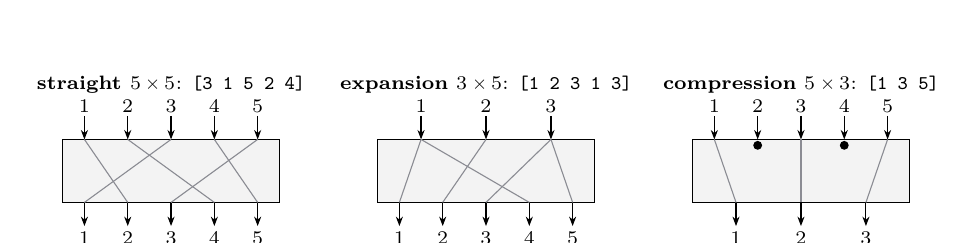
\begin{tikzpicture}[font=\scriptsize,x=5.5mm,y=5mm]
  % straight 5x5: table [3 1 5 2 4]
  \begin{scope}
    \draw[fill=gray!8] (0.5,0) rectangle (5.5,-1.6);
    \node at (3,1.4) {\textbf{straight $5 \times 5$}: \ttx{[3 1 5 2 4]}};
    \foreach \i in {1,...,5} {\draw[-{Stealth[length=1.2mm]}] (\i,0.6) -- (\i,0); \node at (\i,0.85) {\i};
                              \draw[-{Stealth[length=1.2mm]}] (\i,-1.6) -- (\i,-2.2); \node at (\i,-2.5) {\i};}
    \foreach \o/\s in {1/3,2/1,3/5,4/2,5/4} \draw[gray!80!black] (\s,0) -- (\o,-1.6);
  \end{scope}
  % expansion 3x5: table [1 2 3 1 3]
  \begin{scope}[xshift=40mm]
    \draw[fill=gray!8] (0.5,0) rectangle (5.5,-1.6);
    \node at (3,1.4) {\textbf{expansion $3 \times 5$}: \ttx{[1 2 3 1 3]}};
    \foreach \i/\x in {1/1.5,2/3,3/4.5} {\draw[-{Stealth[length=1.2mm]}] (\x,0.6) -- (\x,0); \node at (\x,0.85) {\i};}
    \foreach \i in {1,...,5} {\draw[-{Stealth[length=1.2mm]}] (\i,-1.6) -- (\i,-2.2); \node at (\i,-2.5) {\i};}
    \foreach \o/\x in {1/1.5,2/3,3/4.5,4/1.5,5/4.5} \draw[gray!80!black] (\x,0) -- (\o,-1.6);
  \end{scope}
  % compression 5x3: table [1 3 5]
  \begin{scope}[xshift=80mm]
    \draw[fill=gray!8] (0.5,0) rectangle (5.5,-1.6);
    \node at (3,1.4) {\textbf{compression $5 \times 3$}: \ttx{[1 3 5]}};
    \foreach \i in {1,...,5} {\draw[-{Stealth[length=1.2mm]}] (\i,0.6) -- (\i,0); \node at (\i,0.85) {\i};}
    \foreach \i/\x in {1/1.5,2/3,3/4.5} {\draw[-{Stealth[length=1.2mm]}] (\x,-1.6) -- (\x,-2.2); \node at (\x,-2.5) {\i};}
    \foreach \o/\s in {1.5/1,3/3,4.5/5} \draw[gray!80!black] (\s,0) -- (\o,-1.6);
    \foreach \s in {2,4} \fill (\s,-0.15) circle (1.6pt);
  \end{scope}
\end{tikzpicture}
\end{center}

\textbf{Invertibility.} A straight P-box is invertible: since every input appears exactly once in the table, each output position can be sent back to where it came from. The inverse table is found by writing, for each input position $i$, the output position that holds it. A compression P-box is \emph{not} invertible, because a blocked input bit is simply lost and the inverse would have to invent its value. An expansion P-box is \emph{not} invertible either: an input copied to two outputs would have two candidate sources in the reverse direction, and if the received bits disagree there is no definite answer (more precisely, its reverse is a compression, not an inverse). \imp{Only straight P-boxes are invertible.} This is exactly why AES (all components invertible) uses only straight permutations, while DES (Feistel) can afford an expansion P-box inside its round function.

\begin{worked}[: designing and inverting a straight P-box (slide example)]
\textbf{Q.} Design an $8 \times 8$ permutation table for a straight P-box that moves the two middle bits (bits 4 and 5) of the input to the two ends (bits 1 and 8) of the output, without changing the relative positions of the other bits. Give the inverse table and apply the P-box to \ttx{10011100}.

\textbf{A.} Output bit 1 must take input bit 4 and output bit 8 must take input bit 5. The remaining outputs 2--7 take inputs 1, 2, 3, 6, 7, 8 in their original order. Hence the table is
\[
\text{\ttx{[4 1 2 3 6 7 8 5]}}.
\]
\emph{Inverse:} input 1 went to output 2, input 2 to 3, input 3 to 4, input 4 to 1, input 5 to 8, input 6 to 5, input 7 to 6, input 8 to 7, so the inverse table is \ttx{[2 3 4 1 8 5 6 7]}.\\
\emph{Apply:} input \ttx{10011100} has bits $b_1..b_8 = 1,0,0,1,1,1,0,0$. Output $= b_4 b_1 b_2 b_3 b_6 b_7 b_8 b_5 = \mathbf{11001001}$.\\
\emph{Check:} applying the inverse table to \ttx{11001001} returns \ttx{10011100}; the number of 1s (four) is unchanged, as it must be for any P-box.
\end{worked}

\subsubsection*{S-boxes}
An \textbf{S-box} (substitution box) is a miniature substitution cipher on a few bits: it takes an $n$-bit input and produces an $m$-bit output, where $m$ and $n$ need not be equal. It is normally given as a \textbf{lookup table}: some input bits select the row, the rest select the column, and the cell holds the output. In DES, for instance, a 6-bit input chooses one of 4 rows by its two outer bits and one of 16 columns by its four middle bits, and the cell is a 4-bit value.

\textbf{Linear versus nonlinear.} Write the inputs as $x_1..x_n$ and the outputs as $y_1..y_m$. The S-box is \textbf{linear} if every output is an XOR of inputs, $y_i = a_{i1}x_1 \oplus a_{i2}x_2 \oplus \dots \oplus a_{in}x_n$ with constants $a_{ij} \in \{0,1\}$; then the whole box is a matrix product over GF(2). For example, $y_1 = x_1 \oplus x_2 \oplus x_3$, $y_2 = x_1$ is linear, with matrix $\left(\begin{smallmatrix}1&1&1\\1&0&0\end{smallmatrix}\right)$. If any output contains a product of inputs, such as $y_1 = x_1 x_3 \oplus x_2$, the box is \textbf{nonlinear}. A cipher built only from linear boxes, XORs and P-boxes would be linear as a whole, so every ciphertext bit would be a fixed XOR of plaintext and key bits, and a handful of known plaintext--ciphertext pairs would give a solvable linear system for the key. \imp{The S-boxes are the only nonlinear part of a block cipher, and they must be nonlinear.}

\textbf{Invertibility.} An S-box can be inverted only if it is a one-to-one map, which requires $m = n$ (a $6 \to 4$ box maps 64 inputs onto 16 outputs, so each output has 4 preimages). The slides' $3 \times 3$ example uses the leftmost bit as the row and the two rightmost bits as the column:
\begin{center}\small
\begin{tabular}{@{}c|cccc@{}}
enc & 00 & 01 & 10 & 11\\ \midrule
0 & 011 & 101 & 111 & 100\\
1 & 000 & 010 & 001 & 110\\
\end{tabular}
\qquad
\begin{tabular}{@{}c|cccc@{}}
dec & 00 & 01 & 10 & 11\\ \midrule
0 & 100 & 110 & 101 & 000\\
1 & 011 & 001 & 111 & 010\\
\end{tabular}
\end{center}
Input \ttx{001} (row 0, column 01) encrypts to \ttx{101}, and \ttx{101} (row 1, column 01) in the decryption table gives back \ttx{001}; a script confirms that the two tables undo each other for all 8 inputs.

\subsubsection*{XOR, circular shift, swap, split and combine}
\textbf{Exclusive-or} is addition in GF$(2^n)$, and five properties make it the standard way to mix in a key: \textbf{closure} (the XOR of two $n$-bit words is an $n$-bit word), \textbf{associativity}, \textbf{commutativity}, an \textbf{identity} $00\dots0$, and an \textbf{inverse} for every word, namely the word itself, since $x \oplus x = 00\dots0$. The last property is the important one: whatever is XORed in can be removed by XORing the same value again, $(x \oplus k) \oplus k = x$. A key mixed in this way is called a \textbf{whitener}.

A \textbf{circular shift} rotates an $n$-bit word left or right by $k$ positions. It is invertible, since a left shift by $k$ is undone by a right shift by $k$, and shifting by $k$ is the same as shifting by $k \bmod n$. A \textbf{swap} is the special circular shift by $k = n/2$, exchanging the left and right halves; doing it twice restores the word, so it is \textbf{self-invertible}. A \textbf{split} cuts an $n$-bit word into two $n/2$-bit halves and a \textbf{combine} concatenates two halves; each is the inverse of the other.

\subsection{Product ciphers: confusion, diffusion and rounds \hot}
\likely{One-line theory: ``Define confusion and diffusion; which component provides which?'' or ``What is the avalanche effect?''}
A single small component is easy to analyse and therefore easy to break; a full-size substitution table is secure but impossible to store. Shannon's answer was the \textbf{product cipher}: a cipher that alternates substitutions, permutations and key mixing, so that simple and cheap parts combine into a mapping that behaves like a random one. He named the two properties such a cipher must have.

\textbf{Diffusion} \imp{hides the relationship between the ciphertext and the plaintext}: each ciphertext bit should depend on many or all plaintext bits, so that changing one plaintext bit changes many ciphertext bits. This frustrates an attacker who uses ciphertext statistics (letter or bit frequencies) to guess the plaintext, because any local pattern of the plaintext is spread over the whole block.

\textbf{Confusion} \imp{hides the relationship between the ciphertext and the key}: each ciphertext bit should depend on the key in a complicated way, so that changing one key bit changes most ciphertext bits. This frustrates an attacker who uses known ciphertext to solve for the key.

\textbf{Why S-boxes give confusion.} The key enters the cipher only through XOR, and XOR and P-boxes are linear over GF(2). If the cipher had no S-boxes, every ciphertext bit would be a fixed XOR of plaintext bits and key bits, and a few plaintext--ciphertext pairs would give a linear system whose solution is the key. The nonlinear S-box placed after the key mixing breaks this: its output is a nonlinear function of (data $\oplus$ key), so after a few rounds the ciphertext is a high-degree nonlinear function of the key that cannot be solved for. That is precisely confusion.

\textbf{Why P-boxes give diffusion.} Suppose one input bit of a round changes. It enters one S-box, whose output may change in all its bits (say 2 bits for a $2 \times 2$ box). The P-box then sends those changed bits to \emph{different} S-boxes of the next round, where each again changes up to 2 bits, so the change can grow from 1 bit to 2, 4, 8, \dots\ bits in successive rounds. Without the P-box the changed bits would stay inside the same S-box forever and the change would never spread; the permutation between rounds is what carries it across the block. That is diffusion.

\textbf{Avalanche.} The observable result of good confusion and diffusion is the \textbf{avalanche effect}: flipping one bit of the plaintext or of the key flips about half of the ciphertext bits. Section~\ref{sec:des} shows DES going from 1 differing bit to 29 differing bits out of 64.

\textbf{Rounds.} One layer of S-boxes and P-boxes spreads a bit change only a little, so the layer is repeated. An \textbf{iterated product cipher} applies the same \textbf{round} $N$ times; each round consists of a \textbf{key mixer} (whitener, XOR with a round key), a layer of S-boxes and a P-box. The text between two rounds is called the \textbf{middle text}, and a \textbf{key schedule} (round-key generator) derives the round keys $K_1, \dots, K_N$ from the cipher key, so that each round mixes in a different key. Decryption runs $N$ inverse rounds with the round keys in reverse order.
\begin{center}
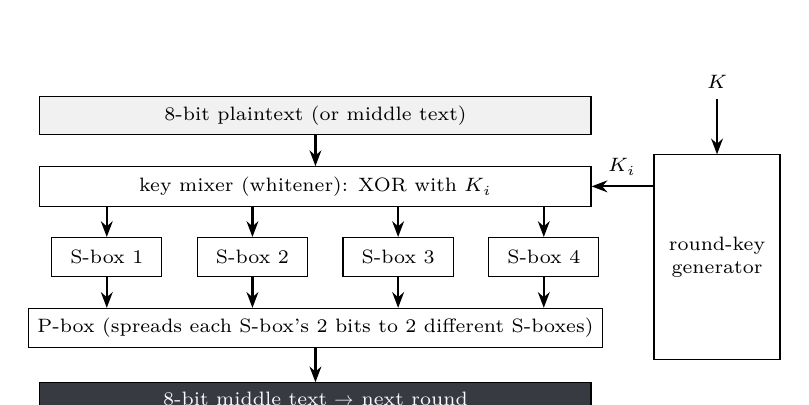
\begin{tikzpicture}[font=\scriptsize,x=1cm,y=1cm]
  \node[draw,fill=gray!10,minimum width=7cm,minimum height=4mm] (pt) at (3.5,0) {8-bit plaintext (or middle text)};
  \node[draw,minimum width=7cm,minimum height=5mm] (km) at (3.5,-0.9) {key mixer (whitener): XOR with $K_i$};
  \foreach \j in {0,...,3} \node[draw,minimum width=1.4cm,minimum height=5mm] (s\j) at (0.85+1.85*\j,-1.8) {S-box \the\numexpr\j+1\relax};
  \node[draw,minimum width=7cm,minimum height=5mm] (pb) at (3.5,-2.7) {P-box (spreads each S-box's 2 bits to 2 different S-boxes)};
  \node[draw,fill=black,text=white,minimum width=7cm,minimum height=4mm] (mt) at (3.5,-3.6) {8-bit middle text $\to$ next round};
  \draw[arr] (pt)--(km); \draw[arr] (pb)--(mt);
  \foreach \j in {0,...,3} {\draw[arr] (km.south -| s\j) -- (s\j); \draw[arr] (s\j) -- (pb.north -| s\j);}
  \node[draw,minimum width=1.6cm,minimum height=2.6cm,align=center] (kg) at (8.6,-1.8) {round-key\\generator};
  \draw[arr] (kg.west |- km) -- node[above]{$K_i$} (km.east);
  \draw[arr] (kg.north) ++(0,0.7) node[above]{$K$} -- (kg.north);
\end{tikzpicture}
\end{center}
\vspace{-2pt}
\centerline{\small One round of the slides' 8-bit product cipher (the slide shows two such rounds).}

\subsection{Feistel ciphers \hot}
\asked{Mid-sem 2024--25 Q6 (5 marks) opens with ``what Feistel structure is prevalent in DES'': the derivation below is that part of the answer.}
Modern block ciphers fall into two classes. \textbf{Feistel ciphers} (DES) use invertible, self-invertible \emph{and noninvertible} components; \textbf{non-Feistel ciphers} (AES) use only invertible components. The problem the Feistel design solves is this: noninvertible components such as an expansion P-box or a $6 \to 4$ S-box mix bits very effectively, but a cipher must be decryptable, and a noninvertible component cannot be run backwards. Feistel's idea is to collect all the noninvertible parts into one function $f$ and never invert it. Its output is only ever \emph{XORed} onto the data, and since XOR is self-inverse, the receiver can cancel it by computing the same $f$ value again and XORing once more.

\textbf{Step 1: the idea in its simplest form.} Let $f$ depend only on the key. Then
\[
\text{encryption: } C = P \oplus f(K), \qquad
\text{decryption: } C \oplus f(K) = P \oplus f(K) \oplus f(K) = P \oplus 00\dots0 = P .
\]
Nothing here requires $f^{-1}$; decryption simply computes $f(K)$ forwards.

\begin{worked}[: the slides' first Feistel example]
\textbf{Q.} Plaintext and ciphertext are 4 bits, the key is 3 bits. $f$ takes the first and third bits of the key, reads them as a decimal number, squares it, and writes the result as 4 bits. Encrypt and decrypt $P = 0111$ with $K = 101$.

\textbf{A.} First and third key bits: $1, 1 \to (11)_2 = 3$; $3^2 = 9 = 1001$, so $f(101) = 1001$.\\
Encryption: $C = P \oplus f(K) = 0111 \oplus 1001 = \mathbf{1110}$.\\
Decryption: $C \oplus f(K) = 1110 \oplus 1001 = 0111 = P$ \checkmark.\\
$f$ is noninvertible (e.g.\ keys $101$ and $111$ both give $1001$, since bit 2 is ignored), yet decryption works because only $f$, never $f^{-1}$, is needed.
\end{worked}

\textbf{Step 2: let the data enter $f$.} A function of the key alone adds nothing per block (it is a fixed XOR, i.e.\ a one-key Vernam). To make $f$ depend on the data while keeping decryption possible, the block is \textbf{split} into a left half $L$ and a right half $R$; $R$ feeds $f$ and $L$ is XORed with the output. This unit is the \textbf{mixer}:
\[
L_2 = L_1 \oplus f(R_1, K), \qquad R_2 = R_1 .
\]
The receiver gets $R_2 = R_1$ unchanged, so it can recompute exactly the same $f(R_1, K)$ and cancel it: $L_2 \oplus f(R_2, K) = L_1 \oplus f(R_1, K) \oplus f(R_1, K) = L_1$. The mixer is therefore \textbf{self-invertible}: applying it twice with the same key is the identity.

\textbf{Step 3: the swapper and more rounds.} The mixer has one flaw: $R$ is never changed, so half of the plaintext appears in clear in the ciphertext. The fix is to add a \textbf{swapper} after the mixer, so that the next round modifies the other half, and to repeat for several rounds. One Feistel round $i$ is then
\[
L_i = R_{i-1}, \qquad R_i = L_{i-1} \oplus f(R_{i-1}, K_i).
\]
\begin{center}
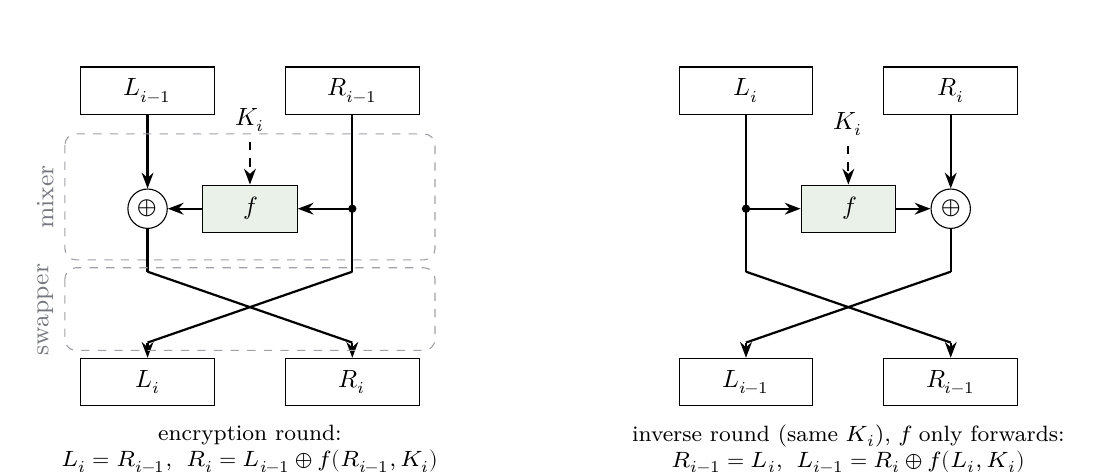
\begin{tikzpicture}[font=\small,x=1cm,y=1cm,hb/.style={draw,minimum width=1.7cm,minimum height=6mm}]
  % ---- left: one Feistel round
  \node[hb] (L0) at (0,0) {$L_{i-1}$};
  \node[hb] (R0) at (2.6,0) {$R_{i-1}$};
  \node[draw,circle,inner sep=0pt,minimum size=5mm] (x) at (0,-1.5) {$\oplus$};
  \node[draw,fill=green!10,minimum width=1.2cm,minimum height=6mm] (f) at (1.3,-1.5) {$f$};
  \draw[arr] (L0) -- (x);
  \draw[thick] (R0) -- (2.6,-2.3);
  \fill (2.6,-1.5) circle (1.5pt);
  \draw[arr] (2.6,-1.5) -- (f);
  \draw[arr] (f) -- (x);
  \draw[arr,dashed] (1.3,-0.65) node[above]{$K_i$} -- (f);
  \draw[thick] (x) -- (0,-2.3);
  \draw[thick] (0,-2.3) -- (2.6,-3.2); \draw[thick] (2.6,-2.3) -- (0,-3.2);
  \node[hb] (L1) at (0,-3.7) {$L_i$};
  \node[hb] (R1) at (2.6,-3.7) {$R_i$};
  \draw[arr] (0,-3.2) -- (L1); \draw[arr] (2.6,-3.2) -- (R1);
  \draw[gray,dashed,rounded corners] (-1.05,-0.55) rectangle (3.65,-2.15);
  \draw[gray,dashed,rounded corners] (-1.05,-2.25) rectangle (3.65,-3.3);
  \node[gray!60!black,rotate=90] at (-1.3,-1.35) {mixer};
  \node[gray!60!black,rotate=90] at (-1.3,-2.78) {swapper};
  \node[align=center,font=\footnotesize] at (1.3,-4.55) {encryption round:\\$L_i = R_{i-1}$,\; $R_i = L_{i-1} \oplus f(R_{i-1}, K_i)$};
  % ---- right: inverse of the round, derived
  \begin{scope}[xshift=7.6cm]
    \node[hb] (a) at (0,0) {$L_i$};
    \node[hb] (b) at (2.6,0) {$R_i$};
    \node[draw,circle,inner sep=0pt,minimum size=5mm] (y) at (2.6,-1.5) {$\oplus$};
    \node[draw,fill=green!10,minimum width=1.2cm,minimum height=6mm] (g) at (1.3,-1.5) {$f$};
    \draw[thick] (a) -- (0,-2.3);
    \fill (0,-1.5) circle (1.5pt);
    \draw[arr] (0,-1.5) -- (g);
    \draw[arr] (g) -- (y);
    \draw[arr] (b) -- (y);
    \draw[arr,dashed] (1.3,-0.7) node[above]{$K_i$} -- (g);
    \draw[thick] (y) -- (2.6,-2.3);
    \draw[thick] (2.6,-2.3) -- (0,-3.2);
    \draw[thick] (0,-2.3) -- (2.6,-3.2);
    \node[hb] (c) at (0,-3.7) {$L_{i-1}$};
    \node[hb] (d) at (2.6,-3.7) {$R_{i-1}$};
    \draw[arr] (0,-3.2) -- (c); \draw[arr] (2.6,-3.2) -- (d);
    \node[align=center,font=\footnotesize] at (1.3,-4.55) {inverse round (same $K_i$), $f$ only forwards:\\$R_{i-1} = L_i$,\; $L_{i-1} = R_i \oplus f(L_i, K_i)$};
  \end{scope}
\end{tikzpicture}
\end{center}

\begin{mustknow}[: why a Feistel round is invertible even if $f$ is not]
Given the round output $(L_i, R_i)$, the first equation hands back $R_{i-1} = L_i$ directly. Knowing $R_{i-1}$, the receiver can \emph{recompute} $f(R_{i-1}, K_i)$ forwards and XOR it away:
\[
R_i \oplus f(L_i, K_i) = L_{i-1} \oplus f(R_{i-1}, K_i) \oplus f(R_{i-1}, K_i) = L_{i-1}.
\]
$f$ is only ever evaluated, never inverted, so it may be many-to-one (expansion P-box, $6 \to 4$ S-boxes). Since the mixer and the swapper are each self-inverse, decryption is the same structure run with the round keys in reverse order ($K_N, \dots, K_1$).
\end{mustknow}

In the slides' two-round final design (slide L7-29), both rounds end with a swapper, so the decryption circuit applies the swapper first and then the mixer, round keys $K_2$ then $K_1$. DES removes the swapper from the \emph{last} round; then encryption and decryption are literally the same algorithm and only the key order changes. The toy below uses that DES convention.

\begin{worked}[: two-round Feistel cipher with a noninvertible $f$]
\textbf{Q.} An 8-bit Feistel cipher has 4-bit halves and two rounds; round 1 has a swapper, round 2 does not (DES convention). The round function is $f(R, K) = (R \oplus K)^2 \bmod 16$. Encrypt $L_0 R_0 = 1010\;0111$ with $K_1 = 0100$, $K_2 = 1001$, then decrypt with the same algorithm and the keys reversed. Show that $f$ is not invertible.

\textbf{A.} $f$ is not invertible: $0011^2 = 9$ and $0101^2 = 25 \equiv 9 \pmod{16}$, so two inputs give $1001$; in fact $x^2 \bmod 16$ only takes the values 0, 1, 4, 9.
\begin{center}\small
\begin{tabular}{@{}lccccc@{}}
\toprule
Round & input $L$, $R$ & $R \oplus K$ & $f$ & $L \oplus f$ & output (after swap?)\\
\midrule
Enc 1 ($K_1 = 0100$) & 1010, 0111 & 0011 & 1001 & 0011 & swap $\to$ 0111, 0011\\
Enc 2 ($K_2 = 1001$) & 0111, 0011 & 1010 & 0100 & 0011 & no swap $\to$ \textbf{0011, 0011}\\
\midrule
Dec 1 ($K_2 = 1001$) & 0011, 0011 & 1010 & 0100 & 0111 & swap $\to$ 0011, 0111\\
Dec 2 ($K_1 = 0100$) & 0011, 0111 & 0011 & 1001 & 1010 & no swap $\to$ \textbf{1010, 0111}\\
\bottomrule
\end{tabular}
\end{center}
Ciphertext $= \mathbf{0011\,0011}$; decryption returns $1010\,0111 = P$ \checkmark. Each decryption round recomputes exactly the $f$ value of the matching encryption round (1001 and 0100), because the half fed to $f$ is passed through unchanged.
\end{worked}

\subsection{Non-Feistel ciphers}
A \textbf{non-Feistel cipher} uses only invertible components, and every component of the encryption has a matching inverse component in the decryption. This constrains the parts: S-boxes must have as many output bits as input bits, and expansion and compression P-boxes are not allowed, because they cannot be inverted. Since there is no $f$ whose output is XORed in, there is also no need to split the block into halves; each round transforms the whole block. The slides' 8-bit product cipher above is a non-Feistel cipher: XOR (self-invertible), $2 \times 2$ invertible S-boxes and a straight P-box, so each round is invertible and decryption runs the inverse rounds with keys $K_2$, $K_1$. AES is the real example.

\begin{center}\small
\begin{tabularx}{\textwidth}{@{}l X X@{}}
\toprule
 & \textbf{Feistel} (DES) & \textbf{Non-Feistel} (AES)\\
\midrule
Components & invertible, self-invertible and noninvertible & only invertible ($n \times n$ S-boxes, straight P-boxes)\\
Block handling & split into $L$, $R$; mixer $L \oplus f(R, K)$, then swapper & whole block in every round\\
Decryption & same structure, round keys reversed; $f$ never inverted & inverse components in reverse order, round keys reversed\\
\bottomrule
\end{tabularx}
\end{center}

\subsection{Attacks on modern block ciphers}
\textbf{Brute force} on the key is normally infeasible because keys are long (but $2^{56}$ for DES is not). The serious attacks exploit the structure of the rounds.
\begin{itemize}
  \item \textbf{Differential cryptanalysis} (Biham and Shamir) is a \textbf{chosen-plaintext} attack. Eve submits pairs of plaintexts with a chosen difference $P_1 \oplus P_2$ and studies the output difference $C_1 \oplus C_2$; a weak cipher propagates certain differences with high probability, which reveals key bits. The slides' extreme case is a cipher that is only an XOR with the key: $C_1 \oplus C_2 = (P_1 \oplus K) \oplus (P_2 \oplus K) = P_1 \oplus P_2$, so the difference passes through untouched and is independent of the key. Nonlinear S-boxes are what destroy this predictability.
  \item \textbf{Linear cryptanalysis} (Matsui) is a \textbf{known-plaintext} attack. If an S-box is not fully nonlinear, some XOR of input and output bits equals an XOR of key bits with probability noticeably different from $1/2$; collecting many plaintext--ciphertext pairs and counting how often such an equation holds reveals those key bits.
\end{itemize}

\subsection{Modern stream ciphers}
A \textbf{modern stream cipher} encrypts and decrypts $r$ bits at a time: the plaintext $P = p_n \dots p_2 p_1$, ciphertext $C = c_n \dots c_2 c_1$ and key stream $K = k_n \dots k_2 k_1$ consist of $r$-bit words, and $c_i = p_i \oplus k_i$, $p_i = c_i \oplus k_i$. Encryption and decryption are a single XOR, so the cipher is fast and needs no padding; all of its security lies in the \textbf{key stream}, which must look random and must never be reused. Stream ciphers are classified by how the key stream is produced.

\textbf{Synchronous stream ciphers.} In a \textbf{synchronous} stream cipher the key stream is \emph{independent} of the plaintext and the ciphertext; it is generated from the key alone, and sender and receiver must stay in step (synchronised) with each other. The ideal case is the \textbf{one-time pad}: a truly random key stream as long as the message, used once, giving perfect secrecy, at the price that a key as long as all the traffic must be shared in advance. Practical synchronous ciphers replace the random pad by a pseudorandom generator such as a \textbf{feedback shift register} (FSR). An FSR has $m$ one-bit cells $b_{m-1} \dots b_1 b_0$; at each step $b_0$ is output as a key bit, all cells shift right, and the new leftmost bit is computed by a \textbf{feedback function} of the old cells. In a \textbf{linear} FSR (LFSR) the feedback is an XOR of selected cells, so it costs one gate. With a well-chosen feedback an $m$-cell LFSR runs through all $2^m - 1$ nonzero states before repeating, the maximum period. Because it is linear, however, about $2m$ consecutive key-stream bits are enough to solve for the feedback taps and predict the rest, so real designs use a \textbf{nonlinear} FSR or combine several LFSRs nonlinearly.

\begin{worked}[: LFSR key stream (Forouzan style)]
\textbf{Q.} Create a 4-cell LFSR with feedback $b_4 = b_1 \oplus b_0$ (the new $b_3$). Show the output for 20 shifts if the seed $b_3 b_2 b_1 b_0$ is $0001$, and find the period.

\textbf{A.} Each step outputs $b_0$, then the state becomes $(b_1 \oplus b_0)\, b_3\, b_2\, b_1$.
\begin{center}\scriptsize\setlength{\tabcolsep}{2.2pt}
\begin{tabular}{@{}l*{16}{c}@{}}
\toprule
step & 0&1&2&3&4&5&6&7&8&9&10&11&12&13&14&15\\
\midrule
state & 0001&1000&0100&0010&1001&1100&0110&1011&0101&1010&1101&1110&1111&0111&0011&\textbf{0001}\\
out $b_0$ & 1&0&0&0&1&0&0&1&1&0&1&0&1&1&1&1\\
\bottomrule
\end{tabular}
\end{center}
At step 15 the state is the seed again, so the key stream repeats with period $\mathbf{15} = 2^4 - 1$ (maximum: every nonzero state appears once). The 20 output bits are $\mathbf{1000\,1001\,1010\,1111\,0001}$.\\
\emph{Check:} the bits 16--20 ($1\,0001$) repeat bits 1--5 ($1\,0001$), as the period predicts.
\end{worked}

\textbf{Nonsynchronous (self-synchronising) stream ciphers.} In a \textbf{nonsynchronous} stream cipher each key-stream element depends on previous plaintext or ciphertext elements. The usual form is \textbf{self-synchronising}: the key stream is computed from the key and the last few ciphertext bits (as in CFB mode). If a ciphertext bit is corrupted or lost, the receiver's key stream is wrong only while the bad bit is inside its window, and decryption recovers by itself once the window has passed.

\textbf{Error behaviour.} In a synchronous cipher a flipped ciphertext bit spoils only the matching plaintext bit, but a lost or inserted bit shifts the two key streams against each other and garbles everything after it until the parties resynchronise. In a self-synchronising cipher a single error spoils a few following bits as well, but a lost bit is recovered from automatically.

\begin{fixbox}
\begin{itemize}
  \item Feistel example (L7 slide 25): the problem says $f$ uses the \emph{first and third} key bits, but the solution ``extracts the first and second bits to get 11''. For $K = 101$ the first and second bits are \ttx{10} $= 2$, giving $f = 0100$; only the first and third bits give \ttx{11} $= 3$ and the stated $f = 1001$, $C = 1110$. Use first and third.
  \item Stream ciphers (L7 slide 39): the line reads ``In a synchronous stream cipher the key is independent of the plaintext or ciphertext''; it is easily read as ``asynchronous'' (the old version of these notes did so). The key-independent class is \textbf{synchronous}. Some books (Stallings) call the \emph{other} class, the self-synchronising ciphers, ``asynchronous'', so do not mix the words up.
  \item Nonlinear S-box (L7 slide 18): over GF(2), $x^3 = x$ and $x^2 = x$, so the slide's $y_1 = x_1^3 + x_2 = x_1 + x_2$ is actually linear; the box is nonlinear because of the product term $x_1 x_2$ in $y_2 = x_1^2 + x_1x_2 + x_3$.
\end{itemize}
\end{fixbox}

% College Lecture 8: DES (Forouzan ch. 6). Every number recomputed by scratchpad/des/verify.py, which implements
% full DES (checked against the Stallings test vector 0123456789ABCDEF/133457799BBCDFF1 -> 85E813540F0AB405).
\section{Data Encryption Standard (DES)}\label{sec:des}

The \textbf{Data Encryption Standard} is the symmetric-key block cipher published by NIST (then NBS) in 1977, based on IBM's Lucifer. It encrypts a \textbf{64-bit block} with a \textbf{56-bit key} through \textbf{16 Feistel rounds}. The key is normally supplied as 64 bits, of which 8 are parity bits that are dropped, and a key schedule derives sixteen \textbf{48-bit round keys} $K_1, \dots, K_{16}$ from it. Decryption is done by the \textbf{reverse cipher}, which is the same algorithm with the round keys used in the order $K_{16}, \dots, K_1$. DES has since been replaced by AES because its key is too short, but its structure is the standard example of a Feistel cipher (Section~\ref{sec:modern}).

\subsection{DES structure \hot}
\asked{2024--25 Q6 (5 marks): Feistel structure, block diagrams of the DES algorithm and the round function, pseudocode for the S-box substitution and key generation.}
Encryption consists of an \textbf{initial permutation} (IP) of the 64-bit plaintext, sixteen rounds, and a \textbf{final permutation} (FP). After IP the block is split into a left half $L_0$ and a right half $R_0$ of 32 bits each. Each round $i$ takes $(L_{i-1}, R_{i-1})$ and produces $(L_i, R_i)$ with a Feistel \textbf{mixer} followed by a \textbf{swapper}:
\[
L_i = R_{i-1}, \qquad R_i = L_{i-1} \oplus f(R_{i-1}, K_i),
\]
where $f$ is the DES function described below. Round 16 has no swapper, and after it the halves are combined and passed through FP to give the 64-bit ciphertext. The block diagrams of the whole algorithm, of one round and of the key generator are drawn in the exam answer at the end of the key-generation subsection.

\subsection{Initial and final permutations}
IP and FP are keyless \textbf{straight P-boxes} ($64 \times 64$) that are inverses of each other: FP $=$ IP$^{-1}$. The IP table is read row by row; entry $j$ is the input bit that goes to output position $j$.
\begin{center}\scriptsize\setlength{\tabcolsep}{3.2pt}
\begin{tabular}{@{}*{8}{c}@{}}
\multicolumn{8}{c}{\textbf{Initial permutation}}\\ \midrule
58&50&42&34&26&18&10&02\\ 60&52&44&36&28&20&12&04\\ 62&54&46&38&30&22&14&06\\ 64&56&48&40&32&24&16&08\\
57&49&41&33&25&17&09&01\\ 59&51&43&35&27&19&11&03\\ 61&53&45&37&29&21&13&05\\ 63&55&47&39&31&23&15&07\\
\end{tabular}
\qquad
\begin{tabular}{@{}*{8}{c}@{}}
\multicolumn{8}{c}{\textbf{Final permutation}}\\ \midrule
40&08&48&16&56&24&64&32\\ 39&07&47&15&55&23&63&31\\ 38&06&46&14&54&22&62&30\\ 37&05&45&13&53&21&61&29\\
36&04&44&12&52&20&60&28\\ 35&03&43&11&51&19&59&27\\ 34&02&42&10&50&18&58&26\\ 33&01&41&09&49&17&57&25\\
\end{tabular}
\end{center}
So output bit 1 of IP is input bit 58, and input bit 1 lands in output position 40; correspondingly the FP table has 40 in position 1 (FP puts it back).

\textbf{Why they add no security.} Both permutations are fixed, keyless and published. An attacker who knows a plaintext can apply IP to it himself, and can apply IP $=$ FP$^{-1}$ to the ciphertext, which strips both permutations off and leaves exactly the 16 rounds to attack. \imp{IP and FP have no cryptographic significance}; they are usually explained as a convenience for loading 8-bit bytes into 1970s hardware.

\begin{worked}[: initial permutation (Forouzan style)]
\textbf{Q.} Find the output of the initial permutation for the input \ttx{0x0002 0000 0000 0001} and show that FP restores it.

\textbf{A.} The input has only two 1-bits: hex digit 4 is \ttx{2} $= 0010$, i.e.\ bit $12 + 3 = \mathbf{15}$, and the last bit, \textbf{64}. In the IP table, 15 is entry 63 and 64 is entry 25, so the output has 1s exactly in positions 25 and 63:
\[
\text{IP}(\ttx{0002000000000001}) = \ttx{0x0000 0080 0000 0002}.
\]
(Bit 25 is the leading bit of hex digit 7, giving \ttx{8}; bit 63 is the third bit of hex digit 16, giving \ttx{2}.)\\
\emph{Check:} in the FP table, entry 15 is 63 and entry 64 is 25, so FP moves bits 63 and 25 back to positions 15 and 64.
\end{worked}

\subsection{Rounds: mixer, swapper and the reverse cipher}
Each round is a Feistel round (Section~\ref{sec:modern}): the \textbf{mixer} replaces $L_{i-1}$ by $L_{i-1} \oplus f(R_{i-1}, K_i)$ and leaves $R_{i-1}$ alone, and the \textbf{swapper} exchanges the halves. The mixer is invertible because of the XOR: given the output, the receiver still has $R_{i-1}$, recomputes $f(R_{i-1}, K_i)$ and XORs it away. The mixer and the swapper are each \textbf{self-inverse}: applying either twice (the mixer with the same key) gives back the input.

\textbf{Why decryption is the same algorithm with keys reversed.} Write encryption as the sequence of operations
\[
\text{IP},\ M_{K_1},\ S,\ M_{K_2},\ S,\ \dots,\ M_{K_{15}},\ S,\ M_{K_{16}},\ \text{FP},
\]
where $M_K$ is the mixer with key $K$ and $S$ the swapper. The inverse of a sequence applies the inverses of its steps in reverse order, and here FP$^{-1} =$ IP, $M_K^{-1} = M_K$, $S^{-1} = S$ and IP$^{-1} =$ FP. Decryption is therefore
\[
\text{IP},\ M_{K_{16}},\ S,\ M_{K_{15}},\ S,\ \dots,\ S,\ M_{K_1},\ \text{FP}.
\]
This is exactly the encryption algorithm with the round keys in the order $K_{16}, \dots, K_1$. The match works only because round 16 has no swapper: with a swapper there, the inverse would start with $S$ and would no longer have the same shape as the cipher. \imp{The last round has no swapper so that the reverse cipher is the cipher itself with reversed round keys.} (Equivalently, Stallings lets all 16 rounds swap and adds a 32-bit swap before FP; the two descriptions give the same ciphertext.)

The slides' pseudocode for the cipher (Forouzan):
\begin{center}
\begin{minipage}{0.8\textwidth}\small
\textbf{Cipher} (plainBlock[64], RoundKeys[16, 48], cipherBlock[64])\\
\{\\
\hspace*{1.5em}\textbf{permute} (64, 64, plainBlock, inBlock, \emph{InitialPermutationTable})\\
\hspace*{1.5em}\textbf{split} (64, 32, inBlock, leftBlock, rightBlock)\\
\hspace*{1.5em}\textbf{for} (round $= 1$ to 16)\\
\hspace*{1.5em}\{\\
\hspace*{3em}\textbf{mixer} (leftBlock, rightBlock, RoundKeys[round])\\
\hspace*{3em}\textbf{if} (round $\neq 16$) \textbf{swapper} (leftBlock, rightBlock)\\
\hspace*{1.5em}\}\\
\hspace*{1.5em}\textbf{combine} (32, 64, leftBlock, rightBlock, outBlock)\\
\hspace*{1.5em}\textbf{permute} (64, 64, outBlock, cipherBlock, \emph{FinalPermutationTable})\\
\}
\end{minipage}
\end{center}
Here mixer does $T \leftarrow f(\text{rightBlock}, K)$, leftBlock $\leftarrow$ leftBlock $\oplus\ T$, and swapper exchanges the two blocks through a temporary copy.

\subsection{The DES function $f(R_{i-1}, K_i)$ \hot}
The DES function is the heart of the cipher and the only place where the key enters. It applies the 48-bit round key to the 32-bit right half and returns 32 bits, through four steps.

\textbf{1. Expansion P-box (32 $\to$ 48).} $R_{i-1}$ has 32 bits but $K_i$ has 48, and the S-boxes need 6-bit inputs, so $R_{i-1}$ is expanded first. It is viewed as eight 4-bit sections; each section is widened to 6 bits by adding, on its left, the last bit of the previous section and, on its right, the first bit of the next section (cyclically, so section 1 borrows bit 32 and section 8 borrows bit 1):
\begin{center}\scriptsize\setlength{\tabcolsep}{3.2pt}
\begin{tabular}{@{}*{6}{c}@{\hspace{14pt}}*{6}{c}@{}}
32&01&02&03&04&05 & 04&05&06&07&08&09\\
08&09&10&11&12&13 & 12&13&14&15&16&17\\
16&17&18&19&20&21 & 20&21&22&23&24&25\\
24&25&26&27&28&29 & 28&29&30&31&32&01\\
\end{tabular}
\end{center}
The 16 bits that appear twice are the first and fourth bits of every section (1, 4, 5, 8, \dots, 29, 32). This duplication is deliberate: a bit at the edge of a section reaches two neighbouring S-boxes, so changing it changes the input of two S-boxes, which is what makes the avalanche grow quickly. Being an expansion P-box, this step is not invertible, which a Feistel cipher can afford.

\textbf{2. Whitener.} The 48-bit expanded half is XORed with the 48-bit round key $K_i$. This is the only point at which the key influences the round.

\textbf{3. S-boxes (48 $\to$ 32).} The 48 bits are cut into eight 6-bit groups, and group $j$ enters S-box $S_j$, which outputs 4 bits. \imp{The S-boxes do the real mixing (confusion)}, being the only nonlinear part of DES. Each S-box is a table of 4 rows and 16 columns. For a 6-bit input $b_1 b_2 b_3 b_4 b_5 b_6$:
\[
\text{row} = (b_1 b_6)_2 \in \{0..3\}, \qquad \text{column} = (b_2 b_3 b_4 b_5)_2 \in \{0..15\},
\]
and the cell is the 4-bit output. The outer bits pick one of four substitutions and the middle bits are substituted by it; every row of every S-box is a permutation of $0..15$ (checked by script), so each output value has exactly 4 preimages and the box as a whole is not invertible. The eight S-boxes are different. S-box 1:
\begin{center}\small\setlength{\tabcolsep}{3.5pt}
\begin{tabular}{@{}c|*{16}{c}@{}}
S1 & 0&1&2&3&4&5&6&7&8&9&10&11&12&13&14&15\\ \midrule
0 & 14&4&13&1&2&15&11&8&3&10&6&12&5&9&0&7\\
1 & 0&15&7&4&14&2&13&1&10&6&12&11&9&5&3&8\\
2 & 4&1&14&8&13&6&2&11&15&12&9&7&3&10&5&0\\
3 & 15&12&8&2&4&9&1&7&5&11&3&14&10&0&6&13\\
\end{tabular}
\end{center}

\textbf{4. Straight P-box (32 $\to$ 32).} The 32 S-box output bits are permuted by a straight P-box; entry $j$ is the input bit sent to output $j$, so the seventh input bit becomes the second output bit:
\begin{center}\scriptsize\setlength{\tabcolsep}{3.2pt}
\begin{tabular}{@{}*{8}{c}@{}}
16&07&20&21&29&12&28&17\\ 01&15&23&26&05&18&31&10\\ 02&08&24&14&32&27&03&09\\ 19&13&30&06&22&11&04&25\\
\end{tabular}
\end{center}
Its job is diffusion: the 4 output bits of each S-box are sent to positions that feed different S-boxes in the next round.

\begin{worked}[: S-box lookup]
\likely{``The input to S-box 1 is \ttx{100011}. What is the output?'' (Forouzan's standard S-box question.)}
\textbf{Q.} (a) The input to S-box 1 is \ttx{100011}. What is the output? (b) The input to S-box 8 is \ttx{000000}. What is the output?

\textbf{A.} (a) Outer bits $b_1 b_6 = 1\,1$, so row $= (11)_2 = 3$. Middle bits $b_2..b_5 = 0001$, so column $= 1$. In S1, row 3, column 1 holds $12$, so the output is $\mathbf{1100}$.\\
(b) Outer bits $0\,0 \Rightarrow$ row 0; middle bits $0000 \Rightarrow$ column 0. S8 row 0 begins \ttx{13 2 8 4 \dots}, so the output is $13 = \mathbf{1101}$.\\
\emph{More S1 lookups for practice:} \ttx{000000} $\to$ row 0, col 0 $\to 14 = 1110$; \ttx{111111} $\to$ row 3, col 15 $\to 13 = 1101$; \ttx{011011} $\to$ row 1, col 13 $\to 5 = 0101$.
\end{worked}

\begin{trap}[: row and column bits]
The row is the \emph{first and last} bit (not the first two), and the column is the \emph{middle four}. Numbering starts at 0 for both rows and columns. Writing the answer as a decimal (12) without converting it to 4 bits (\ttx{1100}) loses the mark that the output is a 4-bit word.
\end{trap}

\begin{worked}[: one full DES round (Forouzan's trace: $P = $ \ttx{123456ABCD132536}, key \ttx{AABB09182736CCDD})]
\textbf{Q.} After the initial permutation, $L_0 = $ \ttx{14A7D678} and $R_0 = $ \ttx{18CA18AD}; the first round key is $K_1 = $ \ttx{194CD072DE8C}. Compute $f(R_0, K_1)$, $L_1$ and $R_1$.

\textbf{A.} $R_0 = 0001\,1000\,1100\,1010\,0001\,1000\,1010\,1101$. Expansion (each 4-bit section borrows its neighbours' edge bits) gives $E(R_0) = $ \ttx{8F16540F155A}; XOR with $K_1$ gives \ttx{965A847DCBD6}. The eight 6-bit groups go through the S-boxes:
\begin{center}\small\setlength{\tabcolsep}{4pt}
\begin{tabular}{@{}lcccccccc@{}}
\toprule
S-box & 1 & 2 & 3 & 4 & 5 & 6 & 7 & 8\\
\midrule
$E(R_0)$ group & 100011 & 110001 & 011001 & 010100 & 000011 & 110001 & 010101 & 011010\\
$K_1$ group & 000110 & 010100 & 110011 & 010000 & 011100 & 101101 & 111010 & 001100\\
XOR (input) & 100101 & 100101 & 101010 & 000100 & 011111 & 011100 & 101111 & 010110\\
row, col & 3, 2 & 3, 2 & 2, 5 & 0, 2 & 1, 15 & 0, 14 & 3, 7 & 0, 11\\
output & 8 & 10 & 15 & 14 & 6 & 5 & 7 & 14\\
\bottomrule
\end{tabular}
\end{center}
S-box output $= $ \ttx{8AFE657E}; the straight P-box gives $f(R_0, K_1) = $ \ttx{4EDF35EC}. Then
\[
L_1 = R_0 = \ttx{18CA18AD}, \qquad R_1 = L_0 \oplus f = \ttx{14A7D678} \oplus \ttx{4EDF35EC} = \ttx{5A78E394}.
\]
\emph{Check:} this is the round-1 output in Forouzan's table; continuing all 16 rounds (round 16 output \ttx{19BA9212 CF26B472}, no swap) and FP gives the ciphertext \ttx{C0B7A8D05F3A829C}, and running the same program with the keys reversed returns the plaintext.
\end{worked}

\subsection{Key generation \hot}
The round-key generator must turn one 56-bit cipher key into sixteen different 48-bit round keys, cheaply and so that every key bit influences many rounds. It works in four steps.
\begin{enumerate}
  \item \textbf{Parity drop (64 $\to$ 56).} The key is supplied as 64 bits in which bits 8, 16, 24, \dots, 64 are parity bits (each key byte has odd parity). A compression permutation (PC-1) discards these 8 bits and permutes the remaining 56.
  \item \textbf{Split.} The 56 bits are split into two 28-bit halves $C_0$ and $D_0$.
  \item \textbf{Shift.} In round $i$ both halves are circularly shifted left, by \textbf{1 bit in rounds 1, 2, 9 and 16} and by 2 bits in all other rounds, giving $C_i$ and $D_i$.
  \item \textbf{Compression P-box (56 $\to$ 48).} $C_i \| D_i$ passes through a compression P-box (PC-2) that blocks 8 of the 56 bits and permutes the other 48; the result is $K_i$.
\end{enumerate}
\textbf{Why it is built this way.} Because the halves are rotated before each compression, a different selection and arrangement of key bits reaches the S-boxes in every round; each key bit ends up in 12 to 15 of the 16 round keys (about 14 on average, counted by script). The shift amounts add up to $4 \times 1 + 12 \times 2 = 28$, a full rotation of a 28-bit half, so $C_{16} = C_0$ and $D_{16} = D_0$. This lets the decryption side generate $K_{16}, \dots, K_1$ on the fly by \emph{right} shifts starting from the original halves.

\begin{worked}[: first round key (same key as the trace above)]
\textbf{Q.} For the key \ttx{AABB09182736CCDD}, find $C_0$, $D_0$, $C_1$, $D_1$ and $K_1$.

\textbf{A.} Parity drop gives the 56-bit key \ttx{C3C033A33F0CFA}, so $C_0 = $ \ttx{C3C033A}, $D_0 = $ \ttx{33F0CFA}. Round 1 shifts by 1 bit:
\begin{center}\small
\begin{tabular}{@{}lll@{}}
$C_0 = 1100\,0011\,1100\,0000\,0011\,0011\,1010$ & $\xrightarrow{\text{rotl } 1}$ & $C_1 = 1000\,0111\,1000\,0000\,0110\,0111\,0101 = $ \ttx{8780675}\\
$D_0 = 0011\,0011\,1111\,0000\,1100\,1111\,1010$ & $\xrightarrow{\text{rotl } 1}$ & $D_1 = 0110\,0111\,1110\,0001\,1001\,1111\,0100 = $ \ttx{67E19F4}\\
\end{tabular}
\end{center}
The compression P-box applied to $C_1 \| D_1$ gives $K_1 = $ \ttx{194CD072DE8C}, the key used in the round trace above.\\
\emph{Check:} in each half the leading bit moved to the end (e.g.\ $C_0$ starts with 1 and $C_1$ ends with 1).
\end{worked}

\begin{worked}[: 2024--25 Q6 (5 marks), answer as it should be written]
\textbf{Q.} In DES, what Feistel structure is prevalent? Use flow diagrams and key generation to define, with block diagrams, (1) the algorithm for DES and (2) the algorithm for the round function. How would you write the pseudocode for the substitution block and key generation?

\textbf{A. Feistel structure.} DES is a Feistel cipher: the 64-bit block (after IP) is split into 32-bit halves, and each of the 16 rounds applies a mixer and a swapper,
\[
L_i = R_{i-1}, \qquad R_i = L_{i-1} \oplus f(R_{i-1}, K_i), \qquad i = 1..16 \text{ (no swap in round 16).}
\]
All noninvertible parts (expansion P-box, $6 \to 4$ S-boxes) are inside $f$, whose output is only XORed in. Since $R_{i-1} = L_i$ is available to the receiver, $L_{i-1} = R_i \oplus f(L_i, K_i)$; so $f$ never has to be inverted, and decryption is the same algorithm with keys $K_{16}, \dots, K_1$.

\textbf{(1) DES algorithm and key generation.}
\begin{center}
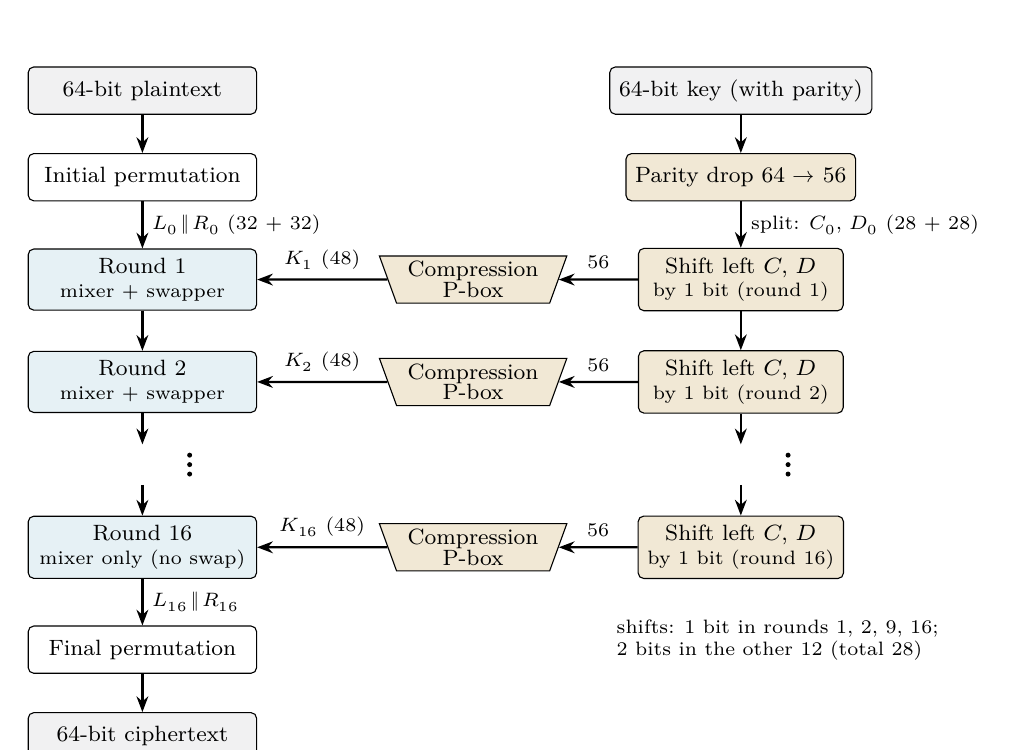
\begin{tikzpicture}[font=\footnotesize,x=1cm,y=1cm,
  db/.style={draw,rounded corners=2pt,minimum width=2.9cm,minimum height=6mm,align=center},
  kb/.style={draw,rounded corners=2pt,fill=yellow!15,minimum width=2.6cm,minimum height=6mm,align=center},
  cb/.style={draw,fill=yellow!15,trapezium,trapezium angle=70,shape border rotate=180,minimum width=2.2cm,minimum height=6mm,align=center,inner sep=1pt}]
  % data path
  \node[db,fill=gray!10] (pt) at (0,0) {64-bit plaintext};
  \node[db] (ip) at (0,-1.1) {Initial permutation};
  \node[db,fill=cyan!8] (r1) at (0,-2.4) {Round 1\\[-1pt]\scriptsize mixer + swapper};
  \node[db,fill=cyan!8] (r2) at (0,-3.7) {Round 2\\[-1pt]\scriptsize mixer + swapper};
  \node[inner sep=0pt,minimum size=5mm] (dd) at (0,-4.75) {}; \foreach \d in {-0.12,0,0.12} \fill (0.6,-4.75+\d) circle (0.9pt);
  \node[db,fill=cyan!8] (r16) at (0,-5.8) {Round 16\\[-1pt]\scriptsize mixer only (no swap)};
  \node[db] (fp) at (0,-7.1) {Final permutation};
  \node[db,fill=gray!10] (ct) at (0,-8.2) {64-bit ciphertext};
  \draw[arr] (pt)--(ip);
  \draw[arr] (ip)-- node[right,font=\scriptsize]{$L_0 \,\|\, R_0$ (32 + 32)} (r1);
  \draw[arr] (r1)--(r2); \draw[arr] (r2)--(dd); \draw[arr] (dd)--(r16);
  \draw[arr] (r16)-- node[right,font=\scriptsize]{$L_{16} \,\|\, R_{16}$} (fp); \draw[arr] (fp)--(ct);
  % key generator
  \node[kb,fill=gray!10] (k64) at (7.6,0) {64-bit key (with parity)};
  \node[kb] (pd) at (7.6,-1.1) {Parity drop 64 $\to$ 56};
  \node[kb] (s1) at (7.6,-2.4) {Shift left $C$, $D$\\[-1pt]\scriptsize by 1 bit (round 1)};
  \node[kb] (s2) at (7.6,-3.7) {Shift left $C$, $D$\\[-1pt]\scriptsize by 1 bit (round 2)};
  \node[inner sep=0pt,minimum size=5mm] (kd) at (7.6,-4.75) {}; \foreach \d in {-0.12,0,0.12} \fill (8.2,-4.75+\d) circle (0.9pt);
  \node[kb] (s16) at (7.6,-5.8) {Shift left $C$, $D$\\[-1pt]\scriptsize by 1 bit (round 16)};
  \node[cb] (c1) at (4.2,-2.4) {Compression\\[-2pt]P-box};
  \node[cb] (c2) at (4.2,-3.7) {Compression\\[-2pt]P-box};
  \node[cb] (c16) at (4.2,-5.8) {Compression\\[-2pt]P-box};
  \draw[arr] (k64)--(pd);
  \draw[arr] (pd)-- node[right,font=\scriptsize]{split: $C_0$, $D_0$ (28 + 28)} (s1);
  \draw[arr] (s1)--(s2); \draw[arr] (s2)--(kd); \draw[arr] (kd)--(s16);
  \foreach \s/\c/\r/\k in {s1/c1/r1/1,s2/c2/r2/2,s16/c16/r16/16} {
    \draw[arr] (\s) -- node[above,font=\scriptsize]{56} (\c);
    \draw[arr] (\c) -- node[above,font=\scriptsize]{$K_{\k}$ (48)} (\r);}
  \node[font=\scriptsize,align=left,anchor=north west] at (5.9,-6.6) {shifts: 1 bit in rounds 1, 2, 9, 16;\\2 bits in the other 12 (total 28)};
\end{tikzpicture}
\end{center}

\textbf{(2) Round $i$ and the round function $f(R_{i-1}, K_i)$.}
\begin{center}
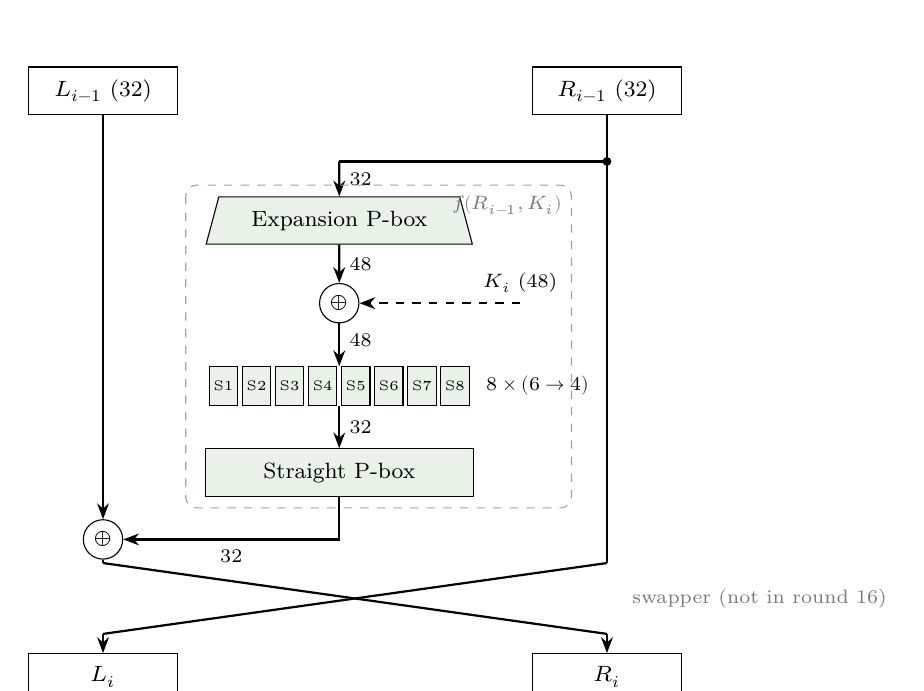
\begin{tikzpicture}[font=\footnotesize,x=1cm,y=1cm,hb/.style={draw,minimum width=1.9cm,minimum height=6mm},
  fb/.style={draw,fill=green!10,minimum width=3.4cm,minimum height=6mm,align=center}]
  \node[hb] (L) at (0,0) {$L_{i-1}$ (32)};
  \node[hb] (R) at (6.4,0) {$R_{i-1}$ (32)};
  \draw[thick] (R) -- (6.4,-6.0);
  \fill (6.4,-0.9) circle (1.6pt);
  \draw[thick] (6.4,-0.9) -- (3,-0.9);
  \node[fb,trapezium,trapezium angle=75,minimum width=2.6cm] (E) at (3,-1.65) {Expansion P-box};
  \draw[arr] (3,-0.9) -- node[right,font=\scriptsize]{32} (E);
  \node[draw,circle,inner sep=0pt,minimum size=5mm] (X) at (3,-2.7) {$\oplus$};
  \draw[arr] (E) -- node[right,font=\scriptsize]{48} (X);
  \draw[arr,dashed] (5.3,-2.7) node[above,font=\scriptsize]{$K_i$ (48)} -- (X);
  \foreach \j in {1,...,8} \node[draw,fill=green!10,minimum width=3.6mm,minimum height=5mm,inner sep=0pt,font=\tiny] (S\j) at (3+0.42*\j-1.89,-3.75) {S\j};
  \draw[arr] (X) -- node[right,font=\scriptsize,pos=0.4]{48} (3,-3.5);
  \node[font=\scriptsize,anchor=west] at (4.75,-3.75) {$8 \times (6 \to 4)$};
  \node[fb] (P) at (3,-4.85) {Straight P-box};
  \draw[arr] (3,-4.0) -- node[right,font=\scriptsize]{32} (P);
  \draw[gray,dashed,rounded corners] (1.05,-1.2) rectangle (5.95,-5.3);
  \node[gray!60!black,anchor=north east,font=\scriptsize] at (5.95,-1.2) {$f(R_{i-1}, K_i)$};
  \node[draw,circle,inner sep=0pt,minimum size=5mm] (M) at (0,-5.7) {$\oplus$};
  \draw[arr] (L) -- (M);
  \draw[arr] (P.south) |- node[pos=0.75,below,font=\scriptsize]{32} (M.east);
  \draw[thick] (M) -- (0,-6.0);
  \draw[thick] (0,-6.0) -- (6.4,-6.9); \draw[thick] (6.4,-6.0) -- (0,-6.9);
  \node[gray!60!black,font=\scriptsize,anchor=west] at (6.6,-6.45) {swapper (not in round 16)};
  \node[hb] (L2) at (0,-7.45) {$L_i$};
  \node[hb] (R2) at (6.4,-7.45) {$R_i$};
  \draw[arr] (0,-6.9) -- (L2); \draw[arr] (6.4,-6.9) -- (R2);
\end{tikzpicture}
\end{center}
Inside $f$: the expansion P-box widens $R_{i-1}$ from 32 to 48 bits, the whitener XORs in $K_i$, eight S-boxes reduce 48 bits to 32 (row $=$ outer bits, column $=$ middle 4 bits), and a straight P-box permutes the 32 bits.

\textbf{Pseudocode} (Forouzan style; bit arrays are indexed from 1).

\begin{minipage}[t]{0.49\linewidth}\small
\textbf{substitute} (inBlock[48], outBlock[32], \emph{SubstitutionTables}[8, 4, 16])\\
\{\\
\hspace*{1em}\textbf{for} ($i = 1$ to 8)\\
\hspace*{1em}\{\\
\hspace*{2em}$b \leftarrow (i - 1) \times 6$ \hfill // start of group $i$\\
\hspace*{2em}row $\leftarrow 2 \times$ inBlock[$b{+}1$] $+$ inBlock[$b{+}6$]\\
\hspace*{2em}col $\leftarrow 8 \times$ inBlock[$b{+}2$] $+ \ 4 \times$ inBlock[$b{+}3$]\\
\hspace*{4.5em}$+\ 2 \times$ inBlock[$b{+}4$] $+$ inBlock[$b{+}5$]\\
\hspace*{2em}value $\leftarrow$ \emph{SubstitutionTables}[$i$][row][col]\\
\hspace*{2em}$o \leftarrow (i - 1) \times 4$\\
\hspace*{2em}outBlock[$o{+}1$] $\leftarrow$ value / 8;\ \ value $\leftarrow$ value mod 8\\
\hspace*{2em}outBlock[$o{+}2$] $\leftarrow$ value / 4;\ \ value $\leftarrow$ value mod 4\\
\hspace*{2em}outBlock[$o{+}3$] $\leftarrow$ value / 2;\ \ value $\leftarrow$ value mod 2\\
\hspace*{2em}outBlock[$o{+}4$] $\leftarrow$ value\\
\hspace*{1em}\}\\
\}
\end{minipage}\hfill
\begin{minipage}[t]{0.47\linewidth}\small
\textbf{Key\_Generator} (keyWithParities[64], RoundKeys[16, 48], \emph{ShiftTable}[16])\\
\{\\
\hspace*{1em}\textbf{permute} (64, 56, keyWithParities, cipherKey, \emph{ParityDropTable})\\
\hspace*{1em}\textbf{split} (56, 28, cipherKey, leftKey, rightKey)\\
\hspace*{1em}\textbf{for} (round $= 1$ to 16)\\
\hspace*{1em}\{\\
\hspace*{2em}\textbf{shiftLeft} (leftKey, \emph{ShiftTable}[round])\\
\hspace*{2em}\textbf{shiftLeft} (rightKey, \emph{ShiftTable}[round])\\
\hspace*{2em}\textbf{combine} (28, 56, leftKey, rightKey, preRoundKey)\\
\hspace*{2em}\textbf{permute} (56, 48, preRoundKey, RoundKeys[round], \emph{KeyCompressionTable})\\
\hspace*{1em}\}\\
\}\\[2pt]
\emph{ShiftTable} $= [1, 1, 2, 2, 2, 2, 2, 2, 1, 2, 2, 2, 2, 2, 2, 1]$; shiftLeft is a circular left shift of a 28-bit half.
\end{minipage}

\medskip
\emph{Check:} the substitute routine reproduces the S-box output \ttx{8AFE657E} of the round trace above (tested by script).
\end{worked}

\begin{mustknow}[: DES at a glance]
64-bit block, 56-bit key (64 with parity), 16 Feistel rounds, 48-bit round keys. Round: $L_i = R_{i-1}$, $R_i = L_{i-1} \oplus f(R_{i-1}, K_i)$, no swap in round 16. $f$: expansion 32 $\to$ 48, XOR $K_i$, 8 S-boxes $6 \to 4$ (row $= b_1 b_6$, column $= b_2..b_5$), straight P-box 32 $\to$ 32. Keys: parity drop 64 $\to$ 56, split 28 $+$ 28, rotate left 1 bit in rounds 1, 2, 9, 16 and 2 bits otherwise, compression 56 $\to$ 48. Decryption: same algorithm, keys $K_{16}..K_1$.
\end{mustknow}

\subsection{DES analysis: avalanche and completeness}
Two properties are expected of a good block cipher. The \textbf{avalanche effect} means that a small change in the plaintext (or the key) should change many ciphertext bits, about half of them. \textbf{Completeness} means that each ciphertext bit should depend on many plaintext bits. In DES both come from the combination of S-boxes (confusion) and P-boxes, including the expansion that feeds each edge bit to two S-boxes (diffusion), and tests show DES is strong in both.

\begin{worked}[: avalanche in DES (Forouzan's example)]
\textbf{Q.} Encrypt the plaintexts \ttx{0000000000000000} and \ttx{0000000000000001} (differing in one bit) with the key \ttx{22234512987ABB23}. How many ciphertext bits differ?

\textbf{A.} The ciphertexts are \ttx{4789FD476E82A5F1} and \ttx{0A4ED5C15A63FEA3}; their XOR has \textbf{29} one-bits, so a 1-bit change of the plaintext changed 29 of the 64 ciphertext bits. The number of differing bits after each round (script) shows how fast the difference spreads:
\begin{center}\small\setlength{\tabcolsep}{3.4pt}
\begin{tabular}{@{}l*{16}{c}@{}}
\toprule
round & 1&2&3&4&5&6&7&8&9&10&11&12&13&14&15&16\\
\midrule
bits differing & 1&6&20&29&30&33&32&29&32&39&33&28&30&31&30&29\\
\bottomrule
\end{tabular}
\end{center}
After only 3 to 4 rounds the difference is already near the ideal of 32; the remaining rounds keep it there.
\end{worked}

\subsection{Weaknesses of DES}
\textbf{Design of the S-boxes and P-boxes.} Critics point out a few irregularities, none of which has led to a practical attack:
\begin{itemize}
  \item In S-box 4, the last three output bits can be derived in the same way as the first output bit by complementing some of the input bits.
  \item Two specially chosen inputs to the S-box array can produce the same output.
  \item The same output of a single round can be obtained by changing bits in only three neighbouring S-boxes.
  \item The initial and final permutations have no security benefit, and in the expansion P-box the first and fourth bits of every 4-bit section are repeated.
\end{itemize}

\textbf{Key size.} The real weakness is the 56-bit key. A brute-force attack on one ciphertext block must try up to $2^{56} \approx 7.2 \times 10^{16}$ keys. At $10^6$ keys per second on each of $10^6$ parallel chips, i.e.\ $10^{12}$ keys per second, the whole key space takes $2^{56}/10^{12} \approx 72\,058$ seconds $\approx$ \textbf{20 hours} (10 hours on average, since the key is found halfway on average). Networked computers simulate parallel hardware: the slides quote 3500 Internet computers finding an RSA Laboratories challenge key in 120 days, so 42\,000 machines would need $3500 \times 120 / 42\,000 = 10$ days.

\textbf{Weak keys.} A \textbf{weak key} is one for which all 16 round keys are the same. This happens when, after the parity drop, each 28-bit half is all 0s or all 1s, because rotating such a half changes nothing. There are 4 weak keys (verified by script: each gives a single distinct round key):
\begin{center}\small
\begin{tabular}{@{}ll@{}}
\toprule
Key before parity drop (64 bits) & Actual key: $C_0$, $D_0$ (hex)\\
\midrule
\ttx{0101 0101 0101 0101} & \ttx{0000000} \ttx{0000000}\\
\ttx{1F1F 1F1F 0E0E 0E0E} & \ttx{0000000} \ttx{FFFFFFF}\\
\ttx{E0E0 E0E0 F1F1 F1F1} & \ttx{FFFFFFF} \ttx{0000000}\\
\ttx{FEFE FEFE FEFE FEFE} & \ttx{FFFFFFF} \ttx{FFFFFFF}\\
\bottomrule
\end{tabular}
\end{center}
With all round keys equal, the key order $K_{16}, \dots, K_1$ is the same as $K_1, \dots, K_{16}$, so the reverse cipher \emph{is} the cipher: \imp{encrypting twice with a weak key returns the plaintext}, $E_K(E_K(P)) = P$.

\textbf{Semi-weak keys.} A \textbf{semi-weak key} creates only 2 distinct round keys, each used 8 times (each half follows the alternating pattern $0101\dots$ or $1010\dots$, or is constant, with at least one half alternating). They come in \textbf{6 pairs} $(k_1, k_2)$ whose round-key sequences are each other's reverse, so $E_{k_2}(E_{k_1}(P)) = P$: one key of the pair decrypts what the other encrypts. The pairs (all checked by script) are:
\begin{center}\small
\begin{tabular}{@{}ll@{\hspace{2.5em}}ll@{}}
\toprule
First key & Second key & First key & Second key\\
\midrule
\ttx{01FE 01FE 01FE 01FE} & \ttx{FE01 FE01 FE01 FE01} & \ttx{1FFE 1FFE 0EFE 0EFE} & \ttx{FE1F FE1F FE0E FE0E}\\
\ttx{1FE0 1FE0 0EF1 0EF1} & \ttx{E01F E01F F10E F10E} & \ttx{011F 011F 010E 010E} & \ttx{1F01 1F01 0E01 0E01}\\
\ttx{01E0 01E0 01F1 01F1} & \ttx{E001 E001 F101 F101} & \ttx{E0FE E0FE F1FE F1FE} & \ttx{FEE0 FEE0 FEF1 FEF1}\\
\bottomrule
\end{tabular}
\end{center}

\textbf{Possible weak keys.} Forouzan lists \textbf{48 possible weak keys}, which create only 4 distinct round keys, each used 4 times (halves repeating with period 4, such as $0011\,0011\dots$). Since $2^{56}$ keys contain only $4 + 12 + 48 = 64$ such keys, a randomly chosen key is weak with probability $2^{-50}$, so these keys matter only if they are chosen on purpose.

\textbf{Key complement.} Let $\bar{x}$ be the bitwise complement. Then $E_{\bar K}(\bar P) = \overline{E_K(P)}$. Proof: complementing $K$ complements every round key, and complementing the data complements $R_{i-1}$ and hence its expansion; then $E(\bar R) \oplus \bar K_i = E(R) \oplus K_i$, so the S-box inputs and $f$ are unchanged, and $\bar L \oplus f = \overline{L \oplus f}$, so every half stays complemented through all rounds (checked by script). As a result, a chosen-plaintext attacker who has $C_1 = E_K(P)$ and $C_2 = E_K(\bar P)$ can test two keys with one encryption ($K$ and $\bar K$), halving the brute-force work to $2^{55}$.

\subsection{Multiple DES}
The obvious fix for a short key is to encrypt several times with different keys. This only helps because DES is \textbf{not a group}: if for every $K_1$, $K_2$ there were a $K_3$ with $E_{K_2}(E_{K_1}(P)) = E_{K_3}(P)$, double encryption would just be single DES with another key. It has been shown that no such $K_3$ exists in general, so cascading DES really produces new mappings.

\textbf{Double DES.} $C = E_{K_2}(E_{K_1}(P))$ and $P = D_{K_1}(D_{K_2}(C))$, with a 112-bit key $(K_1, K_2)$. One would expect $2^{112}$ trials for a brute-force attack, but the \textbf{meet-in-the-middle attack} (a known-plaintext attack) needs only about $2^{57}$. The derivation starts from the middle text $M$, the value between the two encryptions:
\[
M = E_{K_1}(P) \quad\text{and also}\quad M = D_{K_2}(C).
\]
Given one known pair $(P, C)$, Eve encrypts $P$ under all $2^{56}$ values of $K_1$ and stores the results $M$ in a table sorted by $M$. She then decrypts $C$ under all $2^{56}$ values of $K_2$ and looks up each $D_{K_2}(C)$ in the table. Every match gives a candidate pair $(K_1, K_2)$, since it makes both equations hold. The cost is $2^{56} + 2^{56} = 2^{57}$ DES operations (plus memory for $2^{56}$ entries), instead of $2^{56} \times 2^{56} = 2^{112}$, because the two keys are searched \emph{one after the other} rather than in all combinations. Some matches are false: $2^{112}$ key pairs map to only $2^{64}$ middle values, so about $2^{112}/2^{64} = 2^{48}$ pairs fit one $(P, C)$ by chance; testing the candidates on a second known pair $(P', C')$ leaves about $2^{48}/2^{64} < 1$ false survivor, so the right key is identified. \imp{Double DES raises the work only from $2^{56}$ to $2^{57}$, not to $2^{112}$.}

\textbf{Triple DES with two keys.} $C = E_{K_1}(D_{K_2}(E_{K_1}(P)))$ and $P = D_{K_1}(E_{K_2}(D_{K_1}(C)))$, the \textbf{EDE} (encrypt--decrypt--encrypt) form. The key is 112 bits, and a meet-in-the-middle attack now has to split three stages into one and two, which leaves a $2^{112}$ search on one side, so the attack no longer helps. The middle stage is a \emph{decryption} for compatibility: with $K_1 = K_2$ the first two stages cancel and 3DES becomes single DES, so a 3DES device can talk to an old DES device (checked by script). Two-key 3DES is used in PEM and in the financial standard ANS X9.17 / ISO 8732.

\textbf{Triple DES with three keys.} $C = E_{K_3}(D_{K_2}(E_{K_1}(P)))$ with a 168-bit key. Meet-in-the-middle reduces its effective strength to about $2^{112}$, which is still far beyond brute force; it is used in PGP and S/MIME.

\subsection{Security of DES in one line each}
\begin{itemize}
  \item \textbf{Brute force:} $2^{56}$ keys ($2^{55}$ with the complement property), feasible with special hardware or networked computers.
  \item \textbf{Differential cryptanalysis:} DES can be broken with $2^{47}$ chosen plaintexts; its S-boxes were evidently designed against this attack, which is why it is no better than brute force in practice.
  \item \textbf{Linear cryptanalysis:} DES can be broken with $2^{43}$ known plaintexts, a newer attack the designers did not anticipate.
\end{itemize}

\begin{fixbox}
\begin{itemize}
  \item The slides' \textbf{substitute} pseudocode (L8 slide 16, as in Forouzan) declares inBlock[32], outBlock[48]; the sizes are swapped (48 bits in, 32 bits out). It also indexes inBlock[$i \times 6 + 1$] with $i = 1..8$, which reaches position 49 for $i = 8$; the group offset must be $(i - 1) \times 6$ (and $(i - 1) \times 4$ for outBlock), as in the corrected version in the Q6 answer (verified by script).
  \item Semi-weak key table (L8 slide 23), row 3: \ttx{01E0 01E1 01F1 01F1} should be \ttx{01E0 01E0 01F1 01F1}. \ttx{E1} differs from \ttx{E0} only in the parity bit, so it is the same 56-bit key, but it violates odd parity.
  \item Key-size slide (L8 slide 21): ``In 1977 a team of researchers used 3500 computers \dots\ RSA Laboratories'' should read 1997 (RSA's DES Challenge); DES itself was only published in 1977.
\end{itemize}
\end{fixbox}

% College Lecture 9: AES (Forouzan ch. 7, Stallings ch. 5). Every byte in this file (S-box, SubBytes, ShiftRows,
% MixColumns, AddRoundKey, key expansion, FIPS-197 Appendix B round 1 and ciphertext) recomputed by
% scratchpad/aes/aes_check.py and extra.py; the S-box is generated from GF(2^8) inverse + affine map and matched to FIPS-197.
\providecommand{\aesM}[1]{\left(\begin{tabular}{@{\hspace{2pt}}>{\ttfamily}c@{\hspace{5pt}}>{\ttfamily}c@{\hspace{5pt}}>{\ttfamily}c@{\hspace{5pt}}>{\ttfamily}c@{\hspace{2pt}}}#1\end{tabular}\right)}
\providecommand{\aesB}[1]{\textcolor{acc}{\textbf{#1}}}

\section{Advanced Encryption Standard (AES)}\label{sec:aes}

\textbf{Why DES had to be replaced.} By the late 1990s the 56-bit DES key was within reach of brute force: a $2^{56}$ search is about $7.2 \times 10^{16}$ trials, and a purpose-built machine (EFF, 1998) found a DES key in a few days. Triple DES fixes the key length but runs three DES encryptions per block, which is slow in software, and it keeps DES's 64-bit block, which is too small for encrypting large volumes of data under one key. NIST therefore ran an open competition, judged on three criteria (\emph{security, cost, implementation}), and in 2000 chose \textbf{Rijndael} by Daemen and Rijmen. It was published as the \textbf{Advanced Encryption Standard} (FIPS 197) in December 2001.

\textbf{What kind of cipher it is.} \imp{AES is a symmetric-key, non-Feistel block cipher that encrypts 128-bit blocks with a 128-, 192- or 256-bit key in 10, 12 or 14 rounds.} Non-Feistel means that, unlike DES, the round does not split the block into halves and hide a one-way function inside a swap. Instead every step of the round is itself invertible, and decryption runs the inverse steps in reverse order. Such a design is called a substitution--permutation network: substitution (SubBytes) gives confusion, and permutation plus mixing (ShiftRows, MixColumns) give diffusion.

\subsection{Parameters and data units}
The block is always 128 bits and every round key is always 128 bits, whatever the cipher-key length. Only the number of rounds $N_r$ depends on the key size, because a longer key needs more rounds before every key bit has influenced every state bit. Since one round key is added before round 1 and one in each of the $N_r$ rounds, \imp{the number of round keys is $N_r + 1$}, and each round key is 4 words.
\begin{center}\small
\begin{tabular}{@{}lccccc@{}}
\toprule
Version & Key (bits) & Rounds $N_r$ & Round keys $N_r + 1$ & Key words $4(N_r + 1)$ & Brute force\\
\midrule
AES-128 & 128 & 10 & 11 & 44 ($w_0$--$w_{43}$) & $2^{128}$\\
AES-192 & 192 & 12 & 13 & 52 ($w_0$--$w_{51}$) & $2^{192}$\\
AES-256 & 256 & 14 & 15 & 60 ($w_0$--$w_{59}$) & $2^{256}$\\
\bottomrule
\end{tabular}
\end{center}

\textbf{Data units.} AES names five units. A \emph{bit} is a binary digit; a \emph{byte} is 8 bits and is treated as an element of GF$(2^8)$, written as two hex digits; a \emph{word} is 4 bytes (32 bits), seen either as a row or as a column of 4 bytes; a \emph{block} is 16 bytes (128 bits), $b_0 b_1 \dots b_{15}$; and the \emph{state} is the block arranged as a $4 \times 4$ matrix of bytes $s_{r,c}$, which is what every transformation actually acts on. Each column of the state is one word, so the state is also four words $w_0 w_1 w_2 w_3$ side by side.

\textbf{Block to state.} The 16 bytes fill the state \textbf{column by column}: bytes $b_0..b_3$ form column 0 (top to bottom), $b_4..b_7$ column 1, and so on, so that
\[
s_{r,c} = b_{r + 4c}, \qquad\text{equivalently}\qquad b_i \to s_{\,i \bmod 4,\; \lfloor i/4 \rfloor}.
\]
The reverse mapping reads the state column by column to get the output block. This column-major order matters because MixColumns and AddRoundKey work on columns, so four consecutive input bytes are processed together.

\begin{trap}[: filling the state row-wise]
Writing the 16 bytes \emph{across} the rows is the most common slip. The first four bytes go \emph{down} column 0. With the wrong order every later step (ShiftRows, MixColumns, the key words as columns) gives a wrong answer.
\end{trap}

\begin{worked}[: text block to state (slide Example 1, from Forouzan)]
\textbf{Q.} Show the state for the text block ``AES uses a matrix'', letters coded A $= 00$ to Z $= 25$ in hex, padding with Z.\\[2pt]
\textbf{A.} Removing spaces gives 14 letters, so two bogus Z's make 16: \ttx{AESUSESAMATRIXZZ}. Each letter's number is written in \textbf{hex} (for example M $= 12 = $ \ttx{0C}, R $= 17 = $ \ttx{11}, X $= 23 = $ \ttx{17}, Z $= 25 = $ \ttx{19}):
\begin{center}\small\ttfamily\setlength{\tabcolsep}{3.2pt}
\begin{tabular}{@{}l*{16}{c}@{}}
\rmfamily Text & A&E&S&U&S&E&S&A&M&A&T&R&I&X&Z&Z\\
\rmfamily Hex  & 00&04&12&14&12&04&12&00&0C&00&13&11&08&17&19&19
\end{tabular}
\end{center}
Filling column by column (first four bytes down column 0):
\[
\text{State} = \aesM{00&12&0C&08\\04&04&00&17\\12&12&13&19\\14&00&11&19}
\]
Check: $s_{1,3} = b_{1 + 12} = b_{13} = $ \ttx{17} (the X). The slide prints \ttx{23} here; see the corrections box.
\end{worked}

\subsection{Round structure}
Encryption of AES-128 is one key addition followed by 10 rounds:
\begin{enumerate}
  \item \textbf{Pre-round:} AddRoundKey with round key $K_0 = w_0..w_3$ (the cipher key itself).
  \item \textbf{Rounds 1 to $N_r - 1$:} SubBytes, ShiftRows, MixColumns, AddRoundKey (with $K_i = w_{4i}..w_{4i+3}$).
  \item \textbf{Last round $N_r$:} SubBytes, ShiftRows, AddRoundKey, \textbf{without MixColumns}.
\end{enumerate}

\begin{center}
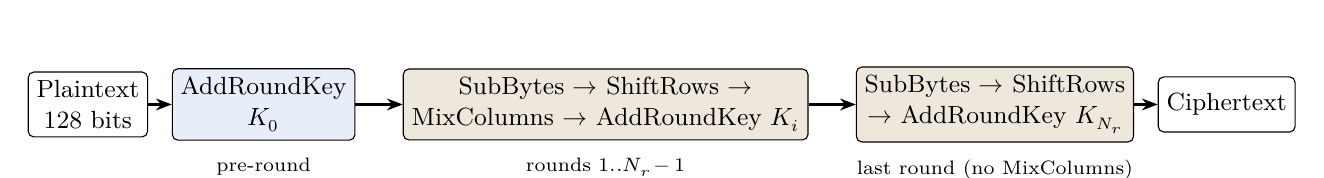
\begin{tikzpicture}[node distance=3mm, every node/.style={font=\footnotesize}]
\node[box] (p) {Plaintext\\128 bits};
\node[box, right=of p, fill=acc!10] (k0) {AddRoundKey\\$K_0$};
\node[box, right=6mm of k0, fill=orange!12] (r) {SubBytes $\to$ ShiftRows $\to$\\MixColumns $\to$ AddRoundKey $K_i$};
\node[box, right=6mm of r, fill=orange!12] (l) {SubBytes $\to$ ShiftRows\\$\to$ AddRoundKey $K_{N_r}$};
\node[box, right=of l] (c) {Ciphertext};
\draw[arr] (p) -- (k0); \draw[arr] (k0) -- (r); \draw[arr] (r) -- (l); \draw[arr] (l) -- (c);
\node[below=1mm of r, font=\scriptsize] {rounds $1..N_r - 1$};
\node[below=1mm of l, font=\scriptsize] {last round (no MixColumns)};
\node[below=1mm of k0, font=\scriptsize] {pre-round};
\end{tikzpicture}
\end{center}

\textbf{Why a key addition comes first.} Every step except AddRoundKey is public and keyless. If the cipher began with SubBytes, an attacker who knows the plaintext could compute that step himself, so it would add work but no secrecy. Adding the key first (key whitening) means that from the very first non-linear step onward, nothing is computable without the key.

\textbf{Why the last round has no MixColumns.} MixColumns is linear over GF$(2^8)$, so $\mathrm{MC}(Y) \oplus K = \mathrm{MC}\big(Y \oplus \mathrm{MC}^{-1}(K)\big)$. If the last round ended with MixColumns and then AddRoundKey, an attacker could apply InvMixColumns to the ciphertext and obtain $Y \oplus \mathrm{MC}^{-1}(K_{N_r})$, which is just the same cipher without the final MixColumns under a different (equally unknown) key. The final MixColumns therefore adds no security. Leaving it out costs nothing and makes the decryption algorithm have the same shape as encryption, which allows the ``equivalent inverse cipher'' to reuse the same hardware.

\begin{mustknow}
AES: block 128, key 128/192/256, rounds 10/12/14, round keys $N_r + 1$ (always 128 bits each), $4(N_r + 1)$ words. Pre-round AddRoundKey; rounds 1..$N_r - 1$: \textbf{SubBytes, ShiftRows, MixColumns, AddRoundKey}; last round drops MixColumns. The state is filled \textbf{column by column}, $s_{r,c} = b_{r + 4c}$.
\end{mustknow}

\subsection{SubBytes (substitution) \hot}
\likely{``Find SubBytes of \ttx{0x53}'' or ``apply SubBytes to the given state using the S-box''; or derive one S-box entry from the GF$(2^8)$ inverse and the affine transform.}

\textbf{Problem and idea.} A cipher built only from XORs, shifts and matrix multiplications is linear, and a linear cipher falls to solving a system of equations. SubBytes is the one non-linear step in AES. Each of the 16 bytes is replaced independently by looking it up in one fixed $16 \times 16$ table, the S-box. Because the same table is used for every byte, \imp{equal input bytes always give equal output bytes}; SubBytes is an \emph{intrabyte} transformation, since a byte's output depends on that byte alone.

\textbf{Lookup rule.} Write the byte as two hex digits $xy$. The \textbf{left digit $x$ selects the row} and the \textbf{right digit $y$ selects the column}; the entry there is the output. For example \ttx{53}: row 5, column 3 gives \ttx{ED}, and \ttx{00}: row 0, column 0 gives \ttx{63}.

\begin{center}
\small\ttfamily\setlength{\tabcolsep}{4pt}\renewcommand{\arraystretch}{1.05}
\begin{tabular}{@{}>{\columncolor{acc!10}}c|*{16}{c}@{}}
\rowcolor{acc!10}$x\backslash y$ & \textbf{0}&\textbf{1}&\textbf{2}&\textbf{3}&\textbf{4}&\textbf{5}&\textbf{6}&\textbf{7}&\textbf{8}&\textbf{9}&\textbf{A}&\textbf{B}&\textbf{C}&\textbf{D}&\textbf{E}&\textbf{F}\\\hline
\textbf{0} & 63 & 7C & 77 & 7B & F2 & 6B & 6F & C5 & 30 & 01 & 67 & 2B & FE & D7 & AB & 76\\
\textbf{1} & CA & 82 & C9 & 7D & FA & 59 & 47 & F0 & AD & D4 & A2 & AF & 9C & A4 & 72 & C0\\
\textbf{2} & B7 & FD & 93 & 26 & 36 & 3F & F7 & CC & 34 & A5 & E5 & F1 & 71 & D8 & 31 & 15\\
\textbf{3} & 04 & C7 & 23 & C3 & 18 & 96 & 05 & 9A & 07 & 12 & 80 & E2 & EB & 27 & B2 & 75\\
\textbf{4} & 09 & 83 & 2C & 1A & 1B & 6E & 5A & A0 & 52 & 3B & D6 & B3 & 29 & E3 & 2F & 84\\
\textbf{5} & 53 & D1 & 00 & ED & 20 & FC & B1 & 5B & 6A & CB & BE & 39 & 4A & 4C & 58 & CF\\
\textbf{6} & D0 & EF & AA & FB & 43 & 4D & 33 & 85 & 45 & F9 & 02 & 7F & 50 & 3C & 9F & A8\\
\textbf{7} & 51 & A3 & 40 & 8F & 92 & 9D & 38 & F5 & BC & B6 & DA & 21 & 10 & FF & F3 & D2\\
\textbf{8} & CD & 0C & 13 & EC & 5F & 97 & 44 & 17 & C4 & A7 & 7E & 3D & 64 & 5D & 19 & 73\\
\textbf{9} & 60 & 81 & 4F & DC & 22 & 2A & 90 & 88 & 46 & EE & B8 & 14 & DE & 5E & 0B & DB\\
\textbf{A} & E0 & 32 & 3A & 0A & 49 & 06 & 24 & 5C & C2 & D3 & AC & 62 & 91 & 95 & E4 & 79\\
\textbf{B} & E7 & C8 & 37 & 6D & 8D & D5 & 4E & A9 & 6C & 56 & F4 & EA & 65 & 7A & AE & 08\\
\textbf{C} & BA & 78 & 25 & 2E & 1C & A6 & B4 & C6 & E8 & DD & 74 & 1F & 4B & BD & 8B & 8A\\
\textbf{D} & 70 & 3E & B5 & 66 & 48 & 03 & F6 & 0E & 61 & 35 & 57 & B9 & 86 & C1 & 1D & 9E\\
\textbf{E} & E1 & F8 & 98 & 11 & 69 & D9 & 8E & 94 & 9B & 1E & 87 & E9 & CE & 55 & 28 & DF\\
\textbf{F} & 8C & A1 & 89 & 0D & BF & E6 & 42 & 68 & 41 & 99 & 2D & 0F & B0 & 54 & BB & 16\\
\end{tabular}\\[2pt]
\rmfamily\small AES S-box (FIPS-197), generated by script from the definition below and checked entry by entry.
\end{center}

\textbf{How the S-box is built.} The table is not arbitrary; each entry is computed in two steps from the byte $a$ viewed as a polynomial in GF$(2^8)$ with modulus $m(x) = x^8 + x^4 + x^3 + x + 1$ (\ttx{11B}).
\begin{enumerate}
  \item \textbf{Multiplicative inverse:} $b = a^{-1}$ in GF$(2^8)$, with \ttx{00} mapped to \ttx{00} (it has no inverse). The inverse map is highly non-linear, which is what resists linear and differential cryptanalysis. This is why AES works in GF$(2^8)$ and not in $\mathbb{Z}_{256}$: in $\mathbb{Z}_{256}$ every even byte lacks an inverse, so the map would not be a permutation.
  \item \textbf{Affine transformation over GF(2):} with $c = \ttx{63} = 0110\,0011$,
  \[
  b'_i = b_i \oplus b_{(i+4) \bmod 8} \oplus b_{(i+5) \bmod 8} \oplus b_{(i+6) \bmod 8} \oplus b_{(i+7) \bmod 8} \oplus c_i, \qquad i = 0..7 .
  \]
  This step breaks the simple algebraic form $a \mapsto a^{-1}$ and removes its fixed points ($00 \mapsto 00$ and $01 \mapsto 01$). As a result the AES S-box has no fixed point ($S(a) \ne a$ for all 256 bytes) and none with $S(a) = \bar{a}$.
\end{enumerate}
InvSubBytes uses the inverse table: undo the affine map, then take the GF$(2^8)$ inverse. Without that table, find the output in the S-box and read off its row and column (for example \ttx{ED} sits at row 5, column 3, so InvSubBytes(\ttx{ED}) $=$ \ttx{53}).

\begin{worked}[: one S-box entry from the definition]
\textbf{Q.} Show that SubBytes(\ttx{53}) $=$ \ttx{ED} by computing it, not by looking it up.\\[2pt]
\textbf{A.} \emph{Step 1.} $\ttx{53} = x^6 + x^4 + x + 1$. Its inverse modulo $m(x)$, by the extended Euclidean algorithm in GF$(2^8)$, is $\ttx{CA} = x^7 + x^6 + x^3 + x$ (check: $\ttx{53} \cdot \ttx{CA} = \ttx{01}$). So $b = \ttx{CA} = 1100\,1010$, that is $b_7..b_0 = 1,1,0,0,1,0,1,0$.\\
\emph{Step 2.} Apply $b'_i = b_i \oplus b_{i+4} \oplus b_{i+5} \oplus b_{i+6} \oplus b_{i+7} \oplus c_i$ (indices mod 8, $c = \ttx{63}$, so $c_0 = c_1 = c_5 = c_6 = 1$):
\begin{center}\small\setlength{\tabcolsep}{5pt}
\begin{tabular}{@{}c|cccccc|c@{}}
\toprule
$i$ & $b_i$ & $b_{i+4}$ & $b_{i+5}$ & $b_{i+6}$ & $b_{i+7}$ & $c_i$ & $b'_i$\\
\midrule
0 & 0 & 0 & 0 & 1 & 1 & 1 & \textbf{1}\\
1 & 1 & 0 & 1 & 1 & 0 & 1 & \textbf{0}\\
2 & 0 & 1 & 1 & 0 & 1 & 0 & \textbf{1}\\
3 & 1 & 1 & 0 & 1 & 0 & 0 & \textbf{1}\\
4 & 0 & 0 & 1 & 0 & 1 & 0 & \textbf{0}\\
5 & 0 & 1 & 0 & 1 & 0 & 1 & \textbf{1}\\
6 & 1 & 0 & 1 & 0 & 0 & 1 & \textbf{1}\\
7 & 1 & 1 & 0 & 0 & 1 & 0 & \textbf{1}\\
\bottomrule
\end{tabular}
\end{center}
Reading $b'_7..b'_0 = 1110\,1101$ gives \textbf{SubBytes(\ttx{53}) $=$ \ttx{ED}}, which matches row 5, column 3 of the table.
\end{worked}

\begin{worked}[: SubBytes of a state (slide Example 2)]
\textbf{Q.} Apply SubBytes to the state of Example 1.\\[2pt]
\textbf{A.} Each byte is looked up independently (row $=$ left digit, column $=$ right digit): \ttx{00}$\to$\ttx{63}, \ttx{04}$\to$\ttx{F2}, \ttx{12}$\to$\ttx{C9}, \ttx{14}$\to$\ttx{FA}, \ttx{0C}$\to$\ttx{FE}, \ttx{13}$\to$\ttx{7D}, \ttx{11}$\to$\ttx{82}, \ttx{08}$\to$\ttx{30}, \ttx{17}$\to$\ttx{F0}, \ttx{19}$\to$\ttx{D4}.
\[
\aesM{00&12&0C&08\\04&04&00&17\\12&12&13&19\\14&00&11&19}
\xrightarrow{\ \text{SubBytes}\ }
\aesM{63&C9&FE&30\\F2&F2&63&\aesB{F0}\\C9&C9&7D&D4\\FA&63&82&D4}
\]
The two \ttx{04}'s in row 1 both become \ttx{F2}, showing that SubBytes alone does not hide repeated bytes; ShiftRows and MixColumns are needed for that.
\end{worked}
Single-bit changes spread: \ttx{5A} and \ttx{5B} differ in one bit, but $S(\ttx{5A}) = \ttx{BE}$ and $S(\ttx{5B}) = \ttx{39}$ differ in four bits ($\ttx{BE} \oplus \ttx{39} = \ttx{87} = 1000\,0111$).

\subsection{ShiftRows (permutation) \hot}
\asked{2025--26 Q4(a) (part of 6 marks): ShiftRows on a given state. Solved in full after AddRoundKey below.}

\textbf{Problem and idea.} SubBytes changes each byte on its own, and MixColumns (next) mixes only the four bytes inside one column. Without a step that moves bytes \emph{between} columns, the four columns would never interact, and AES would be four independent 32-bit ciphers running side by side, each attackable separately. ShiftRows is that step: it permutes bytes so that each column's four bytes end up in four different columns.

\textbf{Mechanism.} \imp{Row $r$ of the state is rotated cyclically left by $r$ bytes}: row 0 is unchanged, row 1 moves left by 1, row 2 by 2, row 3 by 3. In symbols $s'_{r,c} = s_{r,(c + r) \bmod 4}$. The permutation is at the \emph{byte} level: bytes change position but the bits inside a byte are untouched, unlike DES, whose P-boxes permute single bits. Since the four bytes of input column $c$ lie in rows 0, 1, 2, 3, they are shifted by 0, 1, 2, 3 places and land in four different columns; after the next MixColumns every output column then depends on all four input columns. InvShiftRows rotates row $r$ \emph{right} by $r$ bytes.
\[
\begin{pmatrix}s_{00}&s_{01}&s_{02}&s_{03}\\s_{10}&s_{11}&s_{12}&s_{13}\\s_{20}&s_{21}&s_{22}&s_{23}\\s_{30}&s_{31}&s_{32}&s_{33}\end{pmatrix}
\xrightarrow{\ \text{ShiftRows}\ }
\begin{pmatrix}s_{00}&s_{01}&s_{02}&s_{03}\\s_{11}&s_{12}&s_{13}&s_{10}\\s_{22}&s_{23}&s_{20}&s_{21}\\s_{33}&s_{30}&s_{31}&s_{32}\end{pmatrix}
\]
Applied to the SubBytes output of Example 2 (slide Example 3):
\[
\aesM{63&C9&FE&30\\F2&F2&63&F0\\C9&C9&7D&D4\\FA&63&82&D4}
\xrightarrow{\ \text{ShiftRows}\ }
\aesM{63&C9&FE&30\\F2&63&F0&F2\\7D&D4&C9&C9\\D4&FA&63&82}
\]

\subsection{MixColumns (mixing) \hot}
\likely{``Perform MixColumns on one column'' (one or all four output bytes), or ``show that the given column maps to \dots''.}

\textbf{Problem and idea.} SubBytes is intrabyte and ShiftRows only exchanges bytes, so neither makes a byte depend on its neighbours. MixColumns is the \emph{interbyte} step: it replaces each column by a combination of all four of its bytes, so that changing one input byte changes all four output bytes. To guarantee that each new byte differs from the others even when all four inputs are equal, each input is first multiplied by a different constant and then the products are added. This is a matrix multiplication over GF$(2^8)$, where ``add'' is XOR and ``multiply'' is polynomial multiplication modulo \ttx{11B}:
\[
\begin{pmatrix}s'_{0}\\s'_{1}\\s'_{2}\\s'_{3}\end{pmatrix}
= \aesM{02&03&01&01\\01&02&03&01\\01&01&02&03\\03&01&01&02}
\begin{pmatrix}s_{0}\\s_{1}\\s_{2}\\s_{3}\end{pmatrix},
\qquad
\text{InvMixColumns: } \aesM{0E&0B&0D&09\\09&0E&0B&0D\\0D&09&0E&0B\\0B&0D&09&0E}.
\]
Each row of the matrix is the row above rotated right by one. Written out, $s'_0 = 02 \cdot s_0 \oplus 03 \cdot s_1 \oplus s_2 \oplus s_3$, $s'_1 = s_0 \oplus 02 \cdot s_1 \oplus 03 \cdot s_2 \oplus s_3$, $s'_2 = s_0 \oplus s_1 \oplus 02 \cdot s_2 \oplus 03 \cdot s_3$, $s'_3 = 03 \cdot s_0 \oplus s_1 \oplus s_2 \oplus 02 \cdot s_3$. The two matrices multiply to the identity in GF$(2^8)$ (checked by script), which is why InvMixColumns undoes MixColumns.

\textbf{Why the constants 01, 02, 03.} They make encryption cheap, because multiplying by these needs only a shift and XORs. Multiplying by \ttx{02} is multiplying by $x$: shift the byte left by one bit, and if the bit shifted out (the old top bit $b_7$) was 1, the result has an $x^8$ term, which is reduced by XOR with \ttx{1B} (since $x^8 \equiv x^4 + x^3 + x + 1$). This operation is called \textbf{xtime}. Multiplying by \ttx{03} $= x + 1$ is then $(02 \cdot b) \oplus b$. The matrix is also chosen so that the total number of non-zero bytes in an input column plus its output column is at least 5 (branch number 5), so one changed input byte always changes all four output bytes.
\begin{mustknow}[: xtime]
$02 \cdot b = (b \ll 1)$, then XOR \ttx{1B} if the top bit of $b$ was 1. \qquad $03 \cdot b = (02 \cdot b) \oplus b$. \qquad $01 \cdot b = b$.
\end{mustknow}

\begin{worked}[: one column (FIPS-197 test column)]
\textbf{Q.} Apply MixColumns to the column $(\ttx{DB}, \ttx{13}, \ttx{53}, \ttx{45})^T$.\\[2pt]
\textbf{A.} First the products by 02 and 03 of every input byte:
\begin{center}\small\setlength{\tabcolsep}{5pt}
\begin{tabular}{@{}ccccc@{}}
\toprule
$b$ & binary & shift left & top bit 1? & $02 \cdot b$ \;/\; $03 \cdot b = (02 \cdot b) \oplus b$\\
\midrule
\ttx{DB} & 1101\,1011 & 1011\,0110 $=$ \ttx{B6} & yes: $\ttx{B6} \oplus \ttx{1B}$ & \ttx{AD} \;/\; \ttx{76}\\
\ttx{13} & 0001\,0011 & 0010\,0110 $=$ \ttx{26} & no & \ttx{26} \;/\; \ttx{35}\\
\ttx{53} & 0101\,0011 & 1010\,0110 $=$ \ttx{A6} & no & \ttx{A6} \;/\; \ttx{F5}\\
\ttx{45} & 0100\,0101 & 1000\,1010 $=$ \ttx{8A} & no & \ttx{8A} \;/\; \ttx{CF}\\
\bottomrule
\end{tabular}
\end{center}
Then each output byte is a row of the matrix times the column, XORed left to right:
\begin{align*}
s'_0 &= 02{\cdot}\ttx{DB} \oplus 03{\cdot}\ttx{13} \oplus \ttx{53} \oplus \ttx{45} = \ttx{AD} \oplus \ttx{35} \oplus \ttx{53} \oplus \ttx{45} = \ttx{98} \oplus \ttx{53} \oplus \ttx{45} = \ttx{CB} \oplus \ttx{45} = \textbf{\ttx{8E}}\\
s'_1 &= \ttx{DB} \oplus 02{\cdot}\ttx{13} \oplus 03{\cdot}\ttx{53} \oplus \ttx{45} = \ttx{DB} \oplus \ttx{26} \oplus \ttx{F5} \oplus \ttx{45} = \ttx{FD} \oplus \ttx{F5} \oplus \ttx{45} = \ttx{08} \oplus \ttx{45} = \textbf{\ttx{4D}}\\
s'_2 &= \ttx{DB} \oplus \ttx{13} \oplus 02{\cdot}\ttx{53} \oplus 03{\cdot}\ttx{45} = \ttx{DB} \oplus \ttx{13} \oplus \ttx{A6} \oplus \ttx{CF} = \ttx{C8} \oplus \ttx{A6} \oplus \ttx{CF} = \ttx{6E} \oplus \ttx{CF} = \textbf{\ttx{A1}}\\
s'_3 &= 03{\cdot}\ttx{DB} \oplus \ttx{13} \oplus \ttx{53} \oplus 02{\cdot}\ttx{45} = \ttx{76} \oplus \ttx{13} \oplus \ttx{53} \oplus \ttx{8A} = \ttx{65} \oplus \ttx{53} \oplus \ttx{8A} = \ttx{36} \oplus \ttx{8A} = \textbf{\ttx{BC}}
\end{align*}
Answer: $(\ttx{DB}, \ttx{13}, \ttx{53}, \ttx{45}) \to \mathbf{(\ttx{8E}, \ttx{4D}, \ttx{A1}, \ttx{BC})}$, the FIPS-197 test value. Check: every output byte changed, as the branch-number argument predicts.
\end{worked}

A second check comes from the exam state below: column 0 after ShiftRows is $(\ttx{87}, \ttx{6E}, \ttx{46}, \ttx{A6})$. With $02 \cdot \ttx{87} = \ttx{0E} \oplus \ttx{1B} = \ttx{15}$, $03 \cdot \ttx{6E} = \ttx{DC} \oplus \ttx{6E} = \ttx{B2}$, the first output byte is $\ttx{15} \oplus \ttx{B2} \oplus \ttx{46} \oplus \ttx{A6} = \ttx{47}$, and the whole column becomes $(\ttx{47}, \ttx{37}, \ttx{94}, \ttx{ED})$, which is exactly column 0 of the state given in part (b) of that question (Stallings' figures chain ShiftRows $\to$ MixColumns $\to$ AddRoundKey).

\subsection{AddRoundKey (key adding) \hot}
\asked{2025--26 Q4(b) (part of 6 marks): AddRoundKey of a given state with a given key matrix.}

\textbf{Problem and idea.} The three steps above are fixed and public, so on their own they would be a keyless scrambling that anyone can undo. \imp{AddRoundKey is the only step that uses the key}: it XORs the 128-bit round key into the state. It proceeds column by column, like MixColumns, but where MixColumns multiplies each column by a constant matrix, AddRoundKey \emph{adds} a key word to it: in round $i$, column $c$ becomes $s_c \oplus w_{4i + c}$. Equivalently, write the round key as a $4 \times 4$ matrix whose columns are the four words and XOR the two matrices entry by entry.

\textbf{Inverse.} Addition and subtraction in GF$(2^8)$ are both XOR, and $x \oplus k \oplus k = x$, so AddRoundKey is its own inverse; decryption uses the same operation with the same round key.

\textbf{Doing the XOR by hand.} XOR one hex digit at a time, through its 4-bit binary form: $\ttx{4} \oplus \ttx{A} = 0100 \oplus 1010 = 1110 = \ttx{E}$. Useful shortcuts: $x \oplus x = 0$, $x \oplus 0 = x$, $x \oplus \ttx{F}$ flips all four bits.

\begin{worked}[: 2025--26 Q4 (6 marks), Stallings' AES example]
\textbf{Q.} In AES, the state is given below. (a) Show the ShiftRows transformation. (b) After MixColumns, assume the state and the round key are as given. Perform AddRoundKey.\\[2pt]
\textbf{A.} (a) Row $r$ is rotated left by $r$ bytes: row 0 unchanged; row 1 \ttx{EC 6E 4C 90} $\to$ \ttx{6E 4C 90 EC}; row 2 \ttx{4A C3 46 E7} $\to$ \ttx{46 E7 4A C3}; row 3 \ttx{8C D8 95 A6} $\to$ \ttx{A6 8C D8 95}.
\[
\aesM{87&F2&4D&97\\EC&6E&4C&90\\4A&C3&46&E7\\8C&D8&95&A6}
\xrightarrow{\ \text{ShiftRows}\ }
\aesM{87&F2&4D&97\\\aesB{6E}&\aesB{4C}&\aesB{90}&\aesB{EC}\\\aesB{46}&\aesB{E7}&\aesB{4A}&\aesB{C3}\\\aesB{A6}&\aesB{8C}&\aesB{D8}&\aesB{95}}
\]
(b) AddRoundKey is the byte-wise XOR of the state and the key matrix, $s'_{r,c} = s_{r,c} \oplus k_{r,c}$:
\[
\aesM{47&40&A3&4C\\37&D4&70&9F\\94&E4&3A&42\\ED&A5&A6&BC}
\oplus
\aesM{AC&19&28&57\\77&FA&D1&5C\\66&DC&29&00\\F3&21&41&6A}
=
\aesM{\aesB{EB}&\aesB{59}&\aesB{8B}&\aesB{1B}\\\aesB{40}&\aesB{2E}&\aesB{A1}&\aesB{C3}\\\aesB{F2}&\aesB{38}&\aesB{13}&\aesB{42}\\\aesB{1E}&\aesB{84}&\aesB{E7}&\aesB{D6}}
\]
Working, digit by digit (left digits, then right digits):
\begin{center}\footnotesize\ttfamily\setlength{\tabcolsep}{6pt}
\begin{tabular}{@{}llll@{}}
47$\oplus$AC: 4$\oplus$A=E, 7$\oplus$C=B $\to$ EB & 40$\oplus$19: 5, 9 $\to$ 59 & A3$\oplus$28: 8, B $\to$ 8B & 4C$\oplus$57: 1, B $\to$ 1B\\
37$\oplus$77: 4, 0 $\to$ 40 & D4$\oplus$FA: 2, E $\to$ 2E & 70$\oplus$D1: A, 1 $\to$ A1 & 9F$\oplus$5C: C, 3 $\to$ C3\\
94$\oplus$66: F, 2 $\to$ F2 & E4$\oplus$DC: 3, 8 $\to$ 38 & 3A$\oplus$29: 1, 3 $\to$ 13 & 42$\oplus$00: 4, 2 $\to$ 42\\
ED$\oplus$F3: 1, E $\to$ 1E & A5$\oplus$21: 8, 4 $\to$ 84 & A6$\oplus$41: E, 7 $\to$ E7 & BC$\oplus$6A: D, 6 $\to$ D6
\end{tabular}
\end{center}
For example $\ttx{47} \oplus \ttx{AC}$: $0100\,0111 \oplus 1010\,1100 = 1110\,1011 = \ttx{EB}$. Check: XORing the answer with the key again returns the given state (for instance $\ttx{EB} \oplus \ttx{AC} = \ttx{47}$), because AddRoundKey is self-inverse.
\end{worked}

\begin{trap}[: AddRoundKey]
Do not add bytes as integers ($\ttx{47} + \ttx{AC} = \ttx{F3}$ is wrong; the answer is $\ttx{47} \oplus \ttx{AC} = \ttx{EB}$). And in the ShiftRows part, shift \emph{left}, by the row index starting from 0; rotating right, or shifting row 1 by 2, is the usual slip.
\end{trap}

\subsection{Key expansion (AES-128) \hot}
\likely{``Given the cipher key, find $w_4$--$w_7$ (the first round key)'', Forouzan/Stallings style, using the S-box table.}

\textbf{Problem.} AES-128 needs 11 round keys of 128 bits, that is 44 words $w_0..w_{43}$, but the user supplies only one 128-bit key. The expansion must be cheap, must spread every key bit into many round-key bits, and must not be linear; otherwise knowing part of one round key would give the others by simple algebra, and keys with patterns (like DES's weak keys) would produce repeating round keys.

\textbf{Mechanism.} The first four words are the cipher key itself, taken 4 bytes at a time: $w_0 = k_0 k_1 k_2 k_3$, $w_1 = k_4..k_7$, and so on. Each later word is the word four positions back XORed with the previous word, except that every fourth word passes the previous word through a non-linear function first:
\[
w_i =
\begin{cases}
w_{i-4} \oplus w_{i-1}, & i \bmod 4 \ne 0,\\[2pt]
w_{i-4} \oplus t_i, \quad t_i = \mathrm{SubWord}\big(\mathrm{RotWord}(w_{i-1})\big) \oplus \mathrm{RCon}[i/4], & i \bmod 4 = 0.
\end{cases}
\]
\begin{itemize}
  \item \textbf{RotWord} rotates the 4 bytes of a word left by one: $[a_0, a_1, a_2, a_3] \to [a_1, a_2, a_3, a_0]$. It is ShiftRows applied to a single row.
  \item \textbf{SubWord} applies the S-box to each of the 4 bytes. It is SubBytes on a single word and supplies the non-linearity.
  \item \textbf{RCon} (round constant) is a word whose rightmost three bytes are zero and whose left byte is $x^{j-1} \bmod m(x)$ for round $j$. Each value is \ttx{02} times the previous one in GF$(2^8)$, so \ttx{01, 02, 04, 08, 10, 20, 40, 80}, then $02 \cdot \ttx{80}$ overflows and is reduced to $\ttx{00} \oplus \ttx{1B} = \ttx{1B}$, and $02 \cdot \ttx{1B} = \ttx{36}$. RCon is different in every round, which breaks the symmetry between rounds, so that no key gives identical round keys.
\end{itemize}
\begin{center}\small
\begin{tabular}{@{}l*{10}{c}@{}}
\toprule
Round $j$ & 1&2&3&4&5&6&7&8&9&10\\
RCon$[j]$ & \ttx{01}&\ttx{02}&\ttx{04}&\ttx{08}&\ttx{10}&\ttx{20}&\ttx{40}&\ttx{80}&\ttx{1B}&\ttx{36}\\
\bottomrule
\end{tabular}\qquad (each followed by \ttx{00 00 00})
\end{center}
Round key $K_j$ is the four words $w_{4j}, w_{4j+1}, w_{4j+2}, w_{4j+3}$, placed as the \emph{columns} of a $4 \times 4$ matrix, so that AddRoundKey can XOR column $c$ with $w_{4j+c}$. For AES-192 and AES-256 the rule is the same with 6 or 8 words per step instead of 4 ($t$ is computed when $i \bmod 6 = 0$ or $i \bmod 8 = 0$); AES-256 additionally applies SubWord alone when $i \bmod 8 = 4$.

\begin{worked}[: first round key (FIPS-197 / Stallings key)]
\textbf{Q.} The AES-128 cipher key is \ttx{2B7E1516 28AED2A6 ABF71588 09CF4F3C}. Find $w_4, w_5, w_6, w_7$.\\[2pt]
\textbf{A.} $w_0 = \ttx{2B7E1516}$, $w_1 = \ttx{28AED2A6}$, $w_2 = \ttx{ABF71588}$, $w_3 = \ttx{09CF4F3C}$.\\
$i = 4$ is a multiple of 4, so compute $t_4$ from $w_3$:
\begin{center}\small
\begin{tabular}{@{}ll@{}}
RotWord$(w_3)$ & \ttx{09 CF 4F 3C} $\to$ \ttx{CF 4F 3C 09}\\
SubWord & $S(\ttx{CF}) = \ttx{8A}$ (row C, col F), $S(\ttx{4F}) = \ttx{84}$, $S(\ttx{3C}) = \ttx{EB}$, $S(\ttx{09}) = \ttx{01}$ $\Rightarrow$ \ttx{8A84EB01}\\
$\oplus$ RCon[1] & $\ttx{8A84EB01} \oplus \ttx{01000000} = t_4 = \ttx{8B84EB01}$
\end{tabular}
\end{center}
Then
\begin{align*}
w_4 &= w_0 \oplus t_4 = \ttx{2B7E1516} \oplus \ttx{8B84EB01} = \textbf{\ttx{A0FAFE17}}\\
w_5 &= w_1 \oplus w_4 = \ttx{28AED2A6} \oplus \ttx{A0FAFE17} = \textbf{\ttx{88542CB1}}\\
w_6 &= w_2 \oplus w_5 = \ttx{ABF71588} \oplus \ttx{88542CB1} = \textbf{\ttx{23A33939}}\\
w_7 &= w_3 \oplus w_6 = \ttx{09CF4F3C} \oplus \ttx{23A33939} = \textbf{\ttx{2A6C7605}}
\end{align*}
As a matrix (words as columns) the round-1 key is
\[K_1 = \aesM{A0&88&23&2A\\FA&54&A3&6C\\FE&2C&39&76\\17&B1&39&05}.\]
Check: these are the FIPS-197 Appendix A values; continuing the same way gives $t_8 = \ttx{52386BE5}$ (RotWord(\ttx{2A6C7605}) $=$ \ttx{6C76052A}, SubWord $=$ \ttx{50386BE5}, RCon $=$ \ttx{02}), $w_8 = \ttx{F2C295F2}$, and finally $w_{43} = \ttx{B6630CA6}$.
\end{worked}

\subsection{One complete round: FIPS-197 example}
Putting the four steps together on the standard test vector (plaintext \ttx{3243F6A8 885A308D 313198A2 E0370734}, the key above) shows what a full round looks like; the mock paper's AES question (Q8) takes its matrices from this trace. The plaintext fills the state column by column, the pre-round XORs it with $K_0$ (the cipher key), and round 1 then gives:
\begingroup\small
\[
\underbrace{\aesM{19&A0&9A&E9\\3D&F4&C6&F8\\E3&E2&8D&48\\BE&2B&2A&08}}_{\text{after } K_0}
\xrightarrow{\text{Sub}}
\aesM{D4&E0&B8&1E\\27&BF&B4&41\\11&98&5D&52\\AE&F1&E5&30}
\xrightarrow{\text{Shift}}
\aesM{D4&E0&B8&1E\\BF&B4&41&27\\5D&52&11&98\\30&AE&F1&E5}
\xrightarrow{\text{Mix}}
\aesM{04&E0&48&28\\66&CB&F8&06\\81&19&D3&26\\E5&9A&7A&4C}
\xrightarrow{\oplus K_1}
\aesM{A4&68&6B&02\\9C&9F&5B&6A\\7F&35&EA&50\\F2&2B&43&49}
\]
\endgroup
After all ten rounds the ciphertext is \ttx{3925841D 02DC09FB DC118597 196A0B32}; a Python AES implementation reproduces this and decrypts it back.

\subsection{Decryption}
Since every step is invertible, decryption applies the inverse steps in reverse order with the round keys in reverse order ($K_{N_r}$ first, $K_0$ last). In the original design (Forouzan's figure) this gives:
\begin{enumerate}
  \item AddRoundKey with $K_{N_r} = w_{40}..w_{43}$.
  \item Each of the first $N_r - 1$ decryption rounds: InvShiftRows, InvSubBytes, AddRoundKey, InvMixColumns.
  \item Last decryption round: InvShiftRows, InvSubBytes, AddRoundKey with $K_0$ (no InvMixColumns).
\end{enumerate}
InvShiftRows rotates right, InvSubBytes uses the inverse S-box, InvMixColumns uses the matrix [\ttx{0E 0B 0D 09}] and AddRoundKey is its own inverse. Because InvShiftRows and InvSubBytes commute (one moves bytes, the other changes each byte on its own) and InvMixColumns is linear, the steps can be reordered into the same pattern as encryption (InvSubBytes, InvShiftRows, InvMixColumns, AddRoundKey) if the middle round keys are passed through InvMixColumns; this is the \emph{equivalent inverse cipher}. Unlike DES, AES decryption is a different algorithm from encryption, and InvMixColumns, with its larger constants, is slower than MixColumns.

\subsection{Analysis of AES}
\textbf{Brute force.} A 128-bit key needs up to $2^{128}$ trials against DES's $2^{56}$, so if DES can be broken in $t$ seconds, AES-128 needs $2^{128} / 2^{56} \cdot t = 2^{72}\,t$ seconds. The 192- and 256-bit versions widen the gap further. The best published shortcut (biclique attack, 2011) lowers the AES-128 cost only to about $2^{126}$, which is still far out of reach.

\textbf{No weak keys.} DES has keys whose 16 round keys are all equal, so encrypting twice decrypts. In AES, SubWord makes the key schedule non-linear and RCon makes each round's step different, so no such keys are known.

\textbf{Diffusion and statistical attacks.} The steps work together to spread a single change over the whole block in two rounds. In round 1 a changed byte stays one byte through SubBytes and ShiftRows, then MixColumns spreads it to all 4 bytes of its column. In round 2 ShiftRows sends those 4 bytes to 4 different columns, and MixColumns spreads each of them over its column, so all 16 bytes have changed (checked by script: 4 bytes after one round, 16 after two). With 10 or more rounds the ciphertext shows no frequency pattern of the plaintext, and statistical analysis has failed.

\textbf{Differential and linear cryptanalysis.} AES was designed after these attacks were known; the S-box (GF$(2^8)$ inverse) has low differential and linear probabilities, and the branch number of MixColumns forces many active S-boxes over a few rounds, so no such attack works on full AES.

\textbf{Simplicity and cost.} The steps are byte operations, table lookups and XORs, so AES is fast on cheap 8-bit processors with little memory as well as on 32-bit machines (where SubBytes, ShiftRows and MixColumns can be merged into table lookups), and many processors have AES instructions.

\subsection{AES versus DES}
\begin{center}\small
\begin{tabularx}{\textwidth}{@{}l X X@{}}
\toprule
 & DES & AES\\
\midrule
Structure & Feistel (round function need not be invertible) & non-Feistel SPN (every step invertible)\\
Block size & 64 bits & 128 bits\\
Key size & 56 bits (64 with parity) & 128, 192 or 256 bits\\
Rounds & 16 & 10, 12 or 14\\
Round key & 48 bits, 16 keys & 128 bits, $N_r + 1$ keys\\
Works on & bits (expansion, P-boxes) & bytes in GF$(2^8)$ (state matrix)\\
Non-linearity & eight 6-to-4-bit S-boxes & one 8-to-8-bit S-box (inverse $+$ affine)\\
Permutation & bit-level P-boxes & byte-level ShiftRows\\
Decryption & same algorithm, keys reversed & inverse steps, keys reversed\\
Brute force & $2^{56}$ (broken in practice) & $2^{128}$ or more\\
Weak keys & 4 weak, 12 semi-weak & none known\\
\bottomrule
\end{tabularx}
\end{center}

\begin{fixbox}
\begin{itemize}
  \item \textbf{Example 1, letter X.} The slide writes X as \ttx{23}. X is letter 23 in \emph{decimal}, which is \ttx{17} in hex (the same slide correctly converts M $= 12 \to$ \ttx{0C} and R $= 17 \to$ \ttx{11}). With \ttx{17}, SubBytes gives \ttx{F0}; the slide's \ttx{26} (in Examples 2 and 3) is $S(\ttx{23})$. If the exam reuses the slide's state, say which value you used.
  \item \textbf{S-box, row B, column 1.} The slide's table prints \ttx{CB}; the correct FIPS-197 entry is $S(\ttx{B1}) = \ttx{C8}$. \ttx{CB} already appears at row 5, column 9 ($S(\ttx{59}) = \ttx{CB}$), and an S-box is a permutation, so it cannot appear twice. The inverse table on the next slide is right (InvS(\ttx{C8}) $=$ \ttx{B1}). All other 255 entries of the slide match.
  \item \textbf{ShiftRows rows.} The slide numbers the rows 1 to 4 (``Row 1: no shifting, Row 2: 1-byte left shift, \dots''), while the pseudocode and these notes number them 0 to 3. Either way the top row is not shifted and the bottom row moves left by 3.
\end{itemize}
\end{fixbox}

% College Lecture 12 (asymmetric-key cryptography, RSA) + Forouzan 10.1--10.2. Every number recomputed by script
% (scratchpad/rsa/verify.py, gen.py): key tables, square-and-multiply chains, CRT, attack demos.
\section{Asymmetric-Key Cryptography and RSA \new}\label{sec:rsa}
\likely{New this year, so expect one Forouzan-style numerical: ``$p, q, e$ given: find $n$, $\phi(n)$, $d$; encrypt $P$; decrypt $C$'' (4--6 marks), plus a ``why'' question (proof of correctness, why $e = 2$ fails, one attack).}

\subsection{Why asymmetric-key cryptography exists \new}
\likely{``Differentiate symmetric-key and asymmetric-key cryptography'' / ``Why is symmetric cryptography still needed?'' (2--3 marks).}

In symmetric-key cryptography both parties use the same secret key, so before Alice and Bob can talk privately they must already share a secret. This is the \textbf{key distribution problem}: the key has to travel over a secure channel that usually does not exist, and in a group of $N$ users every pair needs its own key, so $N(N-1)/2$ secret keys must be created and stored (4950 for 100 users). Symmetric cryptography also cannot prove who sent a message, because anyone who can decrypt can also encrypt.

\textbf{Asymmetric-key} (public-key) cryptography removes the shared secret. Bob generates a \textbf{key pair}: a \textbf{public key} that he announces to everyone and a \textbf{private key} that only he knows. \imp{The public key locks; the private key unlocks.} Anyone can encrypt for Bob with his public key, but only his private key decrypts, so Alice needs no earlier contact with Bob and $N$ users need only $N$ key pairs. Formally $C = f(K_{\text{public}}, P)$ and $P = g(K_{\text{private}}, C)$, where $f$ is used only for encryption and $g$ only for decryption, and knowing $f$ must not reveal $g$. The secret is now carried by the receiver alone; for Bob to reply, he uses \emph{Alice's} public key. Plaintext and ciphertext are treated as \textbf{numbers}, and encryption is a number-theoretic function rather than substitution and permutation of symbols.

Asymmetric cryptography does \textbf{not} replace symmetric cryptography, because it is far slower: one RSA operation is a modular exponentiation with 1024--2048-bit numbers, while AES needs a few table lookups and XORs per byte (RSA is roughly a thousand times slower). It is therefore used where symmetric cryptography cannot work: \textbf{exchanging a secret session key, authentication and digital signatures}. In practice the two are combined: a random AES key is sent encrypted under the receiver's RSA key, and the bulk data is encrypted with AES under that key.

\begin{center}\small
\begin{tabular}{@{}lll@{}}
\toprule
 & Symmetric-key & Asymmetric-key\\
\midrule
Keys & one shared secret key & public/private key pair\\
Keys for $N$ users & $N(N-1)/2$ & $N$ pairs\\
Secret held by & both parties & receiver only\\
Based on & substitution, permutation & number theory (factoring, discrete log)\\
Speed & fast (bulk data) & slow (keys, signatures)\\
Examples & DES, AES & RSA, ElGamal, ECC\\
\bottomrule
\end{tabular}
\end{center}

\subsection{Trapdoor one-way functions \new}
\likely{``Define a trapdoor one-way function; give the RSA example (2 marks).}
The design problem is to publish $f$ while keeping $f^{-1}$ hidden. A \textbf{one-way function} (OWF) is a function $y = f(x)$ that is easy to compute, while computing $x = f^{-1}(y)$ from $y$ is computationally infeasible. A \textbf{trapdoor one-way function} (TOWF) has a third property: given $y$ \emph{and a secret} (the trapdoor), $x$ is easy to compute. A public-key cipher needs exactly this: the public key lets everyone evaluate $f$, and the trapdoor is the private key.

\textbf{Multiplication is one-way.} For large primes $p, q$, computing $n = p \times q$ is easy, but recovering $p$ and $q$ from $n$ is the \textbf{factorization problem}, for which no polynomial-time (classical) algorithm is known.

\textbf{$y = x^k \bmod n$ is a trapdoor one-way function.} Given $x$, $k$ and $n$, fast exponentiation (\S\ref{sec:modexp}) computes $y$ in about $2\log_2 k$ multiplications; given only $y$, $k$ and $n$, taking the $k$-th root modulo $n$ is believed to be as hard as factoring $n$. The trapdoor is $k'$ with $k k' \equiv 1 \pmod{\phi(n)}$: then $x = y^{k'} \bmod n$. Computing $k'$ needs $\phi(n) = (p-1)(q-1)$, and computing $\phi(n)$ needs $p$ and $q$, so the trapdoor exists only for whoever chose the primes. RSA is this function with $k = e$ and $k' = d$.

\subsection{RSA: key generation, encryption, decryption \new}
\likely{Write the three algorithms, then run them on small primes.}

RSA (Rivest, Shamir, Adleman, 1977) is the most widely used public-key cryptosystem. Bob builds the trapdoor from two primes and publishes only their product; Alice encrypts by raising the plaintext to the public exponent, and Bob decrypts by raising the ciphertext to the private exponent.

\begin{mustknow}[: RSA]
\textbf{Key generation (Bob)}
\begin{enumerate}[leftmargin=1.6em,itemsep=0pt,topsep=1pt]
  \item Choose two large primes $p \ne q$; compute $n = p \times q$ and $\phi(n) = (p-1)(q-1)$.
  \item Choose $e$ with $1 < e < \phi(n)$ and $\gcd(e, \phi(n)) = 1$.
  \item Compute $d = e^{-1} \bmod \phi(n)$ with the extended Euclidean algorithm, so $e \times d \equiv 1 \pmod{\phi(n)}$.
  \item Public key $(e, n)$, announced. Private key $d$, kept secret (with $p$, $q$, $\phi(n)$).
\end{enumerate}
\textbf{Encryption (Alice)}: $C = P^e \bmod n$, \;with $0 \le P < n$. \qquad \textbf{Decryption (Bob)}: $P = C^d \bmod n$.
\end{mustknow}

Encryption and decryption are each one fast exponentiation, so both are polynomial in the size of $n$. Eve sees $C$, $e$ and $n$ and must compute $P = \sqrt[e]{C} \bmod n$, which is exponential for her unless she can factor $n$. The plaintext must be smaller than $n$, because the result is only known modulo $n$: two plaintexts that differ by $n$ give the same ciphertext. A long message is cut into blocks, each a number less than $n$.

\subsection{Why decryption works: proof of correctness \new}
\likely{``Prove that RSA decryption recovers the plaintext'' (2--3 marks).}

Since $d$ is the inverse of $e$ modulo $\phi(n)$, $ed = 1 + k\,\phi(n)$ for some integer $k$. Decryption computes
\[
C^d \equiv (P^e)^d = P^{ed} = P^{1 + k\phi(n)} = P \cdot \big(P^{\phi(n)}\big)^k \pmod n.
\]
\textbf{Case 1: $\gcd(P, n) = 1$} (almost every $P$). Euler's theorem (\S\ref{sec:fermat}) gives $P^{\phi(n)} \equiv 1 \pmod n$, so $C^d \equiv P \cdot 1^k = P \pmod n$. Since $0 \le P < n$, the reduced result is exactly $P$, not just something congruent to it.

\textbf{Case 2: $\gcd(P, n) \ne 1$.} Euler's theorem does not apply, but the result still holds. Since $0 < P < pq$, $P$ is a multiple of exactly one prime, say $p \mid P$ and $q \nmid P$. Modulo $p$, $P \equiv 0$, so $P^{ed} \equiv 0 \equiv P$. Modulo $q$, Fermat's little theorem gives $P^{q-1} \equiv 1$, and $ed = 1 + k(p-1)(q-1)$, so $P^{ed} = P \cdot (P^{q-1})^{k(p-1)} \equiv P \pmod q$. Since $P^{ed} \equiv P$ modulo both $p$ and $q$, and $p, q$ are coprime, the CRT (\S\ref{sec:primes}) gives $P^{ed} \equiv P \pmod{pq}$. (This is Euler's ``second version'', $P^{k\phi(n)+1} \equiv P \pmod n$ for $n = pq$ and every $P$.) Check: $n = 221 = 13 \cdot 17$, $e = 5$, $d = 77$, $P = 65 = 5 \cdot 13$: $65^5 \bmod 221 = 182$ and $182^{77} \bmod 221 = 65$ \checkmark. Such a $P$ is no practical concern, because finding one would give $\gcd(P, n) = p$ and factor $n$.

\textbf{The two algebraic structures.} RSA works in two places (\S\ref{sec:algebra}). Encryption and decryption use the \textbf{public ring} $R = \langle \mathbb{Z}_n, +, \times \rangle$: $P$ and $C$ can be any element of $\mathbb{Z}_n$ (Case 2 shows non-invertible elements also work), and exponentiation is repeated multiplication, which anyone can do since $n$ is public. Key generation uses the \textbf{private group} $G = \langle \mathbb{Z}_{\phi(n)}^*, \times \rangle$: $e$ must belong to this group, i.e.\ $\gcd(e, \phi(n)) = 1$, so that its inverse $d$ exists in it. Only Bob can build $G$, because knowing $\phi(n)$ is as good as knowing the factors: $p + q = n - \phi(n) + 1$, and $p, q$ are the roots of $x^2 - (p+q)x + n = 0$. For $n = 187$, $\phi = 160$: $p + q = 28$, $x^2 - 28x + 187 = 0$ gives $x = (28 \pm 6)/2 = 17, 11$.

\subsection{The slide examples \new}
\likely{Verify one row by hand, e.g.\ ``with $n = 77$, $e = 13$, find $d$ and encrypt $5$.}
The lecture uses the key $p = 7$, $q = 11$, $e = 13$: $n = 77$, $\phi(n) = 60$, and $d = 37$ because $13 \times 37 = 481 = 8 \cdot 60 + 1$. Alice encrypts $5$ and John encrypts $63$ with the same public key $(13, 77)$; Bob decrypts both with $d = 37$. The table also has the class homework key ($n = 187$) and a small textbook key ($n = 33$); all values were recomputed.
\begin{center}\small
\begin{tabular}{@{}cccccll@{}}
\toprule
$p, q$ & $n$ & $\phi(n)$ & $e$ & $d$ & Encrypt & Decrypt\\
\midrule
7, 11 & 77 & 60 & 13 & 37 & $5^{13} \bmod 77 = 26$ & $26^{37} \bmod 77 = 5$\\
7, 11 & 77 & 60 & 13 & 37 & $63^{13} \bmod 77 = 28$ & $28^{37} \bmod 77 = 63$\\
17, 11 & 187 & 160 & 7 & 23 & $88^{7} \bmod 187 = 11$ & $11^{23} \bmod 187 = 88$\\
3, 11 & 33 & 20 & 7 & 3 & $5^7 \bmod 33 = 14$ & $14^3 \bmod 33 = 5$\\
\bottomrule
\end{tabular}
\end{center}
For the slide key, the $d$-table (\S\ref{sec:exteuclid}) on $(60, 13)$ has quotients $4, 1, 1, 1, 1, 2$ and ends with $r_1 = 1$, $t_1 = -23$, so $d = -23 + 60 = 37$. A negative $t_1$ is normal; add $\phi(n)$, never $n$.

\subsection{Exam-format RSA numericals \hot}
\asked{End-sem 2025--26 Q1(b) (6 marks): $M = 63$, $n = 77$, $e = 13$; find $d$ and the ciphertext by fast exponentiation ($d = 37$, $C = 28$).}
\likely{Exactly this layout: $\phi(n)$, gcd check, $d$-table, two square-and-multiply tables, a check line.}

Every exponentiation below uses repeated squaring (\S\ref{sec:modexp}): write the exponent as a sum of powers of 2, square repeatedly (reducing mod $n$ each time), then multiply the needed powers, reducing after each product.

\begin{worked}[: Stallings/Forouzan, the class homework key]
\textbf{Q.} In RSA, $p = 17$, $q = 11$, $e = 7$. Find $n$, $\phi(n)$ and the private key $d$. Encrypt $P = 88$ and show that decryption recovers it.

\textbf{Keys.} $n = 17 \times 11 = 187$; \;$\phi(n) = 16 \times 10 = 160$. Since $160 = 2^5 \cdot 5$ and $7$ is prime, $\gcd(7, 160) = 1$, so $e = 7$ is valid. $d = 7^{-1} \bmod 160$:
\begin{center}\small
\begin{tabular}{@{}r|rrr|rrr@{}}
\toprule
$q$ & $r_1$ & $r_2$ & $r$ & $t_1$ & $t_2$ & $t$\\
\midrule
22 & 160 & 7 & 6 & 0 & 1 & $-22$\\
1 & 7 & 6 & 1 & 1 & $-22$ & 23\\
6 & 6 & 1 & 0 & $-22$ & 23 & $-160$\\
 & \textbf{1} & 0 & & \textbf{23} & $-160$ & \\
\bottomrule
\end{tabular}
\end{center}
$r_1 = 1$ (inverse exists), $d = t_1 = \mathbf{23}$. Check: $7 \times 23 = 161 = 160 + 1$ \checkmark. Public key $(7, 187)$, private key $23$.

\textbf{Encrypt} $C = 88^7 \bmod 187$, with $7 = 4 + 2 + 1$:
\begin{center}\small
\begin{tabular}{@{}lll@{}}
\toprule
Power & Computation & mod 187\\
\midrule
$88^{1}$ & & 88\\
$88^{2}$ & $88^2 = 7744 = 41\cdot187 + 77$ & 77\\
$88^{4}$ & $77^2 = 5929 = 31\cdot187 + 132$ & 132\\
\bottomrule
\end{tabular}
\end{center}
$88^7 = 88^4 \cdot 88^2 \cdot 88^1$: $132 \cdot 77 = 10164 \equiv 66$; \;$66 \cdot 88 = 5808 \equiv 11$. \;$\Rightarrow C = \mathbf{11}$.

\textbf{Decrypt} $P = 11^{23} \bmod 187$, with $23 = 16 + 4 + 2 + 1$:
\begin{center}\small
\begin{tabular}{@{}lll@{}}
\toprule
Power & Computation & mod 187\\
\midrule
$11^{1}$ & & 11\\
$11^{2}$ & $11^2 = 121$ & 121\\
$11^{4}$ & $121^2 = 14641 = 78\cdot187 + 55$ & 55\\
$11^{8}$ & $55^2 = 3025 = 16\cdot187 + 33$ & 33\\
$11^{16}$ & $33^2 = 1089 = 5\cdot187 + 154$ & 154\\
\bottomrule
\end{tabular}
\end{center}
$154 \cdot 55 = 8470 \equiv 55$; \;$55 \cdot 121 = 6655 \equiv 110$; \;$110 \cdot 11 = 1210 \equiv 88$. \;$\Rightarrow P = \mathbf{88}$ \checkmark\ (the original plaintext).
\end{worked}

\begin{worked}[: new, Forouzan exercise style (only $n$ given)]
\textbf{Q.} Bob's RSA public key is $(e, n) = (5, 221)$. (a) Find his private key. (b) Alice sends $P = 100$; find $C$. (c) Show Bob's decryption.

\textbf{(a)} Eve cannot factor a 1024-bit $n$, but $221$ factors by trial division: $221 = 13 \times 17$. So $\phi(n) = 12 \times 16 = 192 = 2^6 \cdot 3$, and $\gcd(5, 192) = 1$. $d = 5^{-1} \bmod 192$:
\begin{center}\small
\begin{tabular}{@{}r|rrr|rrr@{}}
\toprule
$q$ & $r_1$ & $r_2$ & $r$ & $t_1$ & $t_2$ & $t$\\
\midrule
38 & 192 & 5 & 2 & 0 & 1 & $-38$\\
2 & 5 & 2 & 1 & 1 & $-38$ & 77\\
2 & 2 & 1 & 0 & $-38$ & 77 & $-192$\\
 & \textbf{1} & 0 & & \textbf{77} & $-192$ & \\
\bottomrule
\end{tabular}
\end{center}
$d = \mathbf{77}$. Check: $5 \times 77 = 385 = 2 \cdot 192 + 1$ \checkmark.

\textbf{(b)} $5 = 4 + 1$: \;$100^2 = 10000 = 45 \cdot 221 + 55$; \;$55^2 = 3025 = 13 \cdot 221 + 152$, so $100^4 \equiv 152$. \;$C = 152 \cdot 100 = 15200 = 68 \cdot 221 + 172$ $\Rightarrow C = \mathbf{172}$.

\textbf{(c)} $P = 172^{77} \bmod 221$, with $77 = 64 + 8 + 4 + 1$:
\begin{center}\small
\begin{tabular}{@{}lll@{}}
\toprule
Power & Computation & mod 221\\
\midrule
$172^{1}$ & & 172\\
$172^{2}$ & $172^2 = 29584 = 133\cdot221 + 191$ & 191\\
$172^{4}$ & $191^2 = 36481 = 165\cdot221 + 16$ & 16\\
$172^{8}$ & $16^2 = 256 = 221 + 35$ & 35\\
$172^{16}$ & $35^2 = 1225 = 5\cdot221 + 120$ & 120\\
$172^{32}$ & $120^2 = 14400 = 65\cdot221 + 35$ & 35\\
$172^{64}$ & $35^2 \equiv 120$ (as above) & 120\\
\bottomrule
\end{tabular}
\end{center}
$172^{64} \cdot 172^{8} = 120 \cdot 35 = 4200 = 19 \cdot 221 + 1 \equiv 1$; \;$1 \cdot 16 = 16$; \;$16 \cdot 172 = 2752 = 12 \cdot 221 + 100$. \;$\Rightarrow P = \mathbf{100}$ \checkmark.
\end{worked}

\subsection{Choosing $e$; why $e = 2$ never works \new}
\likely{``Why is $e = 2$ not allowed? or ``is $e = 3$ valid for $p = 19$, $q = 23$? (1--2 marks).}
Encryption cost depends on the number of bits and of 1-bits in $e$, so a small $e$ with few 1-bits makes encryption cheap. The standard choice is $e = 2^{16} + 1 = 65537$: it is prime (so it is coprime to $\phi(n)$ unless a prime factor of $\phi(n)$ is 65537 itself), its binary form $1\,0000\,0000\,0000\,0001$ needs only 16 squarings and one multiplication, and it is large enough to defeat the low-exponent attacks below. The private exponent $d$ is then about as long as $n$, so decryption is the slow side (which the CRT speeds up).

\textbf{$e = 2$ (or any even $e$) is invalid.} Since $p$ and $q$ are odd primes, $p - 1$ and $q - 1$ are even, so $\phi(n)$ is even (in fact divisible by 4). Then $\gcd(2, \phi(n)) = 2 \ne 1$, $e$ is not in $\mathbb{Z}_{\phi(n)}^*$, and no $d$ exists. The cause is that squaring is not one-to-one: $x$ and $n - x$ have the same square, so $C = P^2$ cannot be uniquely undone. The same check catches a Forouzan exercise: $p = 19$, $q = 23$, $e = 3$ gives $\phi(n) = 18 \cdot 22 = 396 = 3 \cdot 132$, so $\gcd(3, 396) = 3$ and $e = 3$ is not allowed for this $n$.

\begin{trap}[: the usual RSA slips]
$d$ is the inverse of $e$ modulo $\boldsymbol{\phi(n)}$, never modulo $n$ (for $(7, 187)$ the answer is $23$; $7^{-1} \bmod 187 = 107$ is useless). Check $\gcd(e, \phi(n)) = 1$ before running the table. The plaintext must satisfy $P < n$. Encrypt with the \emph{receiver's} public key. Reduce mod $n$ after every multiplication, and turn a negative $t_1$ into $t_1 + \phi(n)$.
\end{trap}

\subsection{Faster decryption with the CRT \new}
\likely{``Decrypt using the Chinese remainder theorem'' on a small key, or ``why is CRT decryption about 4 times faster''.}

Decryption is slow because $d$ and $n$ are both full size. Bob, however, knows $p$ and $q$, so he can work modulo each prime separately and combine the answers with the CRT (\S\ref{sec:primes}). Modulo $p$ the exponent can be reduced: since $C^{p-1} \equiv 1 \pmod p$ (Fermat), $C^d \equiv C^{d \bmod (p-1)} \pmod p$. Bob computes
\[
d_p = d \bmod (p-1),\quad d_q = d \bmod (q-1),\qquad P_p = C^{d_p} \bmod p,\quad P_q = C^{d_q} \bmod q,
\]
and then the unique $P < n$ with $P \equiv P_p \pmod p$ and $P \equiv P_q \pmod q$:
\[
P = \big(P_p \cdot q \cdot (q^{-1} \bmod p) + P_q \cdot p \cdot (p^{-1} \bmod q)\big) \bmod n .
\]
Each half uses a modulus of half the length (a multiplication costs about $1/4$) and an exponent of half the length (half as many steps), so each half costs about $1/8$ of the full exponentiation and both together about $1/4$: decryption is roughly \textbf{4 times faster}. Only the key owner can use it, since it needs $p$ and $q$.

\begin{worked}[: CRT decryption of the previous ciphertext]
\textbf{Q.} With $p = 13$, $q = 17$, $d = 77$, decrypt $C = 172$ using the CRT.

$d_p = 77 \bmod 12 = 5$, \;$d_q = 77 \bmod 16 = 13$; \;$C_p = 172 \bmod 13 = 3$, \;$C_q = 172 \bmod 17 = 2$.\\
$P_p = 3^5 \bmod 13 = 243 \bmod 13 = 9$. \;$P_q = 2^{13} \bmod 17$: $2^4 = 16 \equiv -1$, $2^8 \equiv 1$, so $2^{13} = 2^8 \cdot 2^4 \cdot 2 \equiv -2 \equiv 15$.\\
$q^{-1} \bmod p = 17^{-1} \bmod 13 = 4^{-1} \bmod 13 = 10$ \;($4 \cdot 10 = 40 = 3 \cdot 13 + 1$); \;$p^{-1} \bmod q = 13^{-1} \bmod 17 = 4$ \;($13 \cdot 4 = 52 = 3 \cdot 17 + 1$).\\
$P = 9 \cdot 17 \cdot 10 + 15 \cdot 13 \cdot 4 = 1530 + 780 = 2310 = 10 \cdot 221 + 100$ $\Rightarrow P = \mathbf{100}$ \checkmark, the same as $172^{77} \bmod 221$, with exponents 5 and 13 instead of 77.
\end{worked}

\subsection{Attacks on RSA \new}
\likely{``Explain any two attacks on RSA'' or ``why must $p$ and $q$ be large / not close / why OAEP''.}

No devastating attack on correctly used RSA is known; every known attack exploits a weak choice of parameters or a careless use of textbook RSA. The slide's list, each with the reason it works:
\begin{itemize}[leftmargin=1.4em]
  \item \textbf{Factorization.} If Eve factors $n$ she computes $\phi(n)$ and then $d = e^{-1} \bmod \phi(n)$, exactly as Bob did. The whole security rests on $n$ being too large to factor.
  \item \textbf{Chosen-ciphertext.} RSA is multiplicative: $(P_1 P_2)^e = P_1^e P_2^e$. To decrypt $C$, Eve picks $X$, asks Bob to decrypt the innocent-looking $Y = C \cdot X^e \bmod n$, receives $Z = Y^d = P \cdot X$, and computes $P = Z \cdot X^{-1}$. With $(7, 187)$, $C = 11$, $X = 2$: $Y = 11 \cdot 128 \bmod 187 = 99$, $Z = 99^{23} \bmod 187 = 176$, $P = 176 \cdot 94 \bmod 187 = 88$ \checkmark.
  \item \textbf{Low encryption exponent.} If $e$ is small and $P^e < n$, no reduction happens and $P = \sqrt[e]{C}$ over the integers ($e = 3$, $n = 187$, $P = 5$: $C = 125$, $\sqrt[3]{125} = 5$). \textbf{Coppersmith's} theorem extends this to finding small unknown parts of $P$. \textbf{Broadcast}: if the same $P$ goes to $e$ receivers with moduli $n_1, \dots, n_e$, the CRT gives $P^e \bmod n_1 \cdots n_e$, which equals $P^e$ because $P^e < n_1 \cdots n_e$, so an integer root reveals $P$ (with $e = 3$, $n = 55, 391, 1189$ and $P = 42$: ciphertexts $3, 189, 370$, CRT gives $74088 = 42^3$). \textbf{Related messages} (Franklin--Reiter) and \textbf{short pad} attacks similarly recover messages that are linearly related or padded with too few random bits.
  \item \textbf{Low decryption exponent.} A small $d$ speeds decryption but Wiener's attack recovers $d$ from $e/n$ by continued fractions when $d < \tfrac{1}{3} n^{1/4}$. A \textbf{revealed} $d$ is worse than it looks: $n$ with one pair $(e, d)$ lets anyone factor $n$, so all keys on that modulus are dead.
  \item \textbf{Plaintext attacks.} \emph{Short message}: if $P$ comes from a small set (a PIN), Eve encrypts every candidate with the public key and compares, since textbook RSA is deterministic. \emph{Cyclic}: $C$ is a permutation of $\mathbb{Z}_n$, so re-encrypting $C, C^e, C^{e^2}, \dots$ eventually returns to $C$, and the value just before $C$ is $P$; with $(7, 33)$ and $C = 14$: $14 \to 20 \to 26 \to 5 \to 14$, so $P = 5$. \emph{Unconcealed}: some $P$ satisfy $P^e \equiv P$ (always $0$, $1$, $n - 1$); their number is $(1 + \gcd(e-1, p-1))(1 + \gcd(e-1, q-1))$, which for the slide key $(13, 77)$ is $7 \cdot 3 = 21$ messages (e.g.\ $10^{13} \equiv 10$), because $e - 1 = 12$ is a multiple of $p - 1 = 6$.
  \item \textbf{Common modulus.} If two users share $n$ with exponents $e_1, e_2$, $\gcd(e_1, e_2) = 1$, and the same $P$ is sent to both, Eve finds $s e_1 + t e_2 = 1$ and gets $C_1^s C_2^t = P^{s e_1 + t e_2} = P$. With $n = 187$, $e_1 = 3$, $e_2 = 7$, $P = 5$: $C_1 = 125$, $C_2 = 146$, $s = -2$, $t = 1$, $P = (125^{-1})^2 \cdot 146 = 3^2 \cdot 146 = 1314 \equiv 5$ \checkmark. Also, any user of the shared $n$ can factor it from his own $(e, d)$.
  \item \textbf{Implementation (timing, power).} Square-and-multiply does an extra multiplication for every 1-bit of $d$, so the decryption time or power trace leaks the bits of $d$. Defences: constant-time exponentiation, random delays, or \emph{blinding} (decrypt $C \cdot r^e$, then multiply by $r^{-1}$).
\end{itemize}

\subsection{Recommendations}
Each recommendation blocks one of the attacks above.
\begin{itemize}[leftmargin=1.4em]
  \item $n$ at least \textbf{1024 bits} (about 309 decimal digits; 2048 today), so each of $p$, $q$ at least \textbf{512 bits} (about 154 digits). This defeats factorization.
  \item $p$ and $q$ must not be close to each other, otherwise Fermat factoring ($n = a^2 - b^2$ with $a \approx \sqrt n$) finds them quickly. Both $p - 1$ and $q - 1$ should have a large prime factor (against Pollard's $p - 1$ method), and $p/q$ should not be close to a fraction with small numerator and denominator.
  \item The modulus must not be shared between users (common-modulus attack).
  \item $e = 2^{16} + 1$ or an integer close to it (against low-exponent attacks, while keeping encryption fast).
  \item If $d$ leaks, Bob must change $n$, $e$ and $d$, since one $(e, d)$ pair reveals the factors of $n$.
  \item Messages must be padded with \textbf{OAEP} (Optimal Asymmetric Encryption Padding). OAEP mixes the message with a fresh random value $r$ through two hash-based masks ($M_1 = P \oplus G(r)$, $M_2 = r \oplus H(M_1)$) and encrypts $M_1 \| M_2$. This makes RSA probabilistic (same $P$, different $C$ each time), fills the block so $P^e > n$, and destroys the multiplicative structure, blocking the short-message, broadcast, cyclic-style and chosen-ciphertext tricks.
\end{itemize}

\begin{fixbox}
\begin{itemize}[leftmargin=1.2em,itemsep=0pt]
  \item Slide on trapdoor functions: ``there is not a polynomial time solution'' to factoring should read \emph{no polynomial-time classical algorithm is known}; it is not proven impossible (Shor's quantum algorithm is polynomial).
  \item Slide on RSA size: a 512-bit prime has 154 or 155 decimal digits ($2^{511}$ has 154, $2^{512}$ has 155); 1024 bits is 309 digits, as stated.
\end{itemize}
\end{fixbox}

% College Lecture 13 (ElGamal, elliptic curve cryptosystems) + Forouzan 10.4--10.5. Every number recomputed by script
% (scratchpad/rsa/ecc.py, ecc2.py, ecc3.py): ElGamal runs, point lists, every addition/doubling, scalar multiples.
\section{ElGamal and Elliptic Curve Cryptosystems \new}\label{sec:elgamal}
\likely{New this year: an ElGamal encrypt/decrypt with a small prime, ``find all points on $E_p(a, b)$'', one point addition or doubling, and ``why must $r$ be fresh / why ECC has smaller keys''.}

\subsection{ElGamal cryptosystem \new}
\likely{``Explain ElGamal key generation, encryption and decryption; prove decryption is correct; encrypt $P$ with $p, e_1, d, r$ given'' (4--5 marks).}

RSA rests on factoring. ElGamal rests on a different hard problem, the \textbf{discrete logarithm problem} (DLP, \S\ref{sec:primes}). Let $p$ be a large prime and $e_1$ a \textbf{primitive root} of $p$, i.e.\ an element whose powers $e_1^1, e_1^2, \dots, e_1^{p-1}$ run through all of $\mathbb{Z}_p^* = \{1, \dots, p-1\}$ (\S\ref{sec:fermat}). Computing $e_2 = e_1^d \bmod p$ is easy by square-and-multiply, but given $e_1$, $e_2$ and $p$, finding $d = \log_{e_1} e_2 \bmod p$ is infeasible for large $p$. So $d \mapsto e_1^d$ is a one-way function, and Bob's private key is the exponent $d$ hidden inside the public $e_2$.

The idea of encryption is to multiply $P$ by a \textbf{one-time mask} $e_2^r$ that only Bob can rebuild. Alice picks a fresh random $r$ and sends two numbers: $C_1 = e_1^r$, a ``hint'' that reveals nothing about $r$ (DLP again), and $C_2 = P \cdot e_2^r$, the masked plaintext. Bob rebuilds the mask from the hint with his secret: $C_1^d = e_1^{rd} = (e_1^d)^r = e_2^r$. Eve would need either $d$ or $r$, and both are discrete logarithms. This is the Diffie--Hellman idea turned into a cipher: $e_2^r = e_1^{dr}$ is a shared value that Alice computes from $(r, e_2)$ and Bob from $(d, C_1)$.

\begin{mustknow}[: ElGamal]
\textbf{Key generation (Bob)}: choose a large prime $p$ and a primitive root $e_1$ of $p$; choose $d$ with $1 \le d \le p - 2$; compute $e_2 = e_1^d \bmod p$. Public key $(e_1, e_2, p)$, private key $d$.\\
\textbf{Encryption (Alice)}: choose a \textbf{fresh} random $r \in \mathbb{Z}_p^*$; \;$C_1 = e_1^r \bmod p$, \;$C_2 = (P \times e_2^r) \bmod p$. Send $(C_1, C_2)$.\\
\textbf{Decryption (Bob)}: $P = \big[C_2 \times (C_1^d)^{-1}\big] \bmod p$, \;and $(C_1^d)^{-1} = C_1^{\,p-1-d} \bmod p$.
\end{mustknow}

\textbf{Proof of correctness.} $C_2 \times (C_1^d)^{-1} = (P \cdot e_2^r)\,(e_1^{rd})^{-1} = P \cdot e_2^r\,(e_2^r)^{-1} = P \pmod p$, because $e_1^{rd} = (e_1^d)^r = e_2^r$. The inverse exists since $C_1^d \in \mathbb{Z}_p^*$.

\textbf{The inverse shortcut.} By Fermat, $C_1^{p-1} \equiv 1$, so $C_1^d \cdot C_1^{p-1-d} \equiv 1$, i.e.\ $(C_1^d)^{-1} = C_1^{p-1-d}$. One exponentiation replaces an exponentiation followed by an extended-Euclid inverse.

\textbf{Properties.} ElGamal is \textbf{probabilistic}: the same $P$ encrypted twice gives different ciphertexts because $r$ changes, so Eve cannot test guesses by re-encrypting them (unlike textbook RSA). The price is \textbf{ciphertext expansion}: the ciphertext is the pair $(C_1, C_2)$, each as long as $p$, so it is \textbf{twice the size} of the plaintext. Like RSA, it is slow and is used for short data such as session keys.

\begin{worked}[: the slide example]
\textbf{Q.} Bob chooses $p = 11$, $e_1 = 2$, $d = 3$. Find his public key. Alice encrypts $P = 7$ with $r = 4$. Find the ciphertext and show Bob's decryption.

\textbf{Keys.} $2$ is a primitive root of 11 (its powers are $2, 4, 8, 5, 10, 9, 7, 3, 6, 1$). $e_2 = 2^3 \bmod 11 = 8$. Public key $(2, 8, 11)$, private key $3$.\\
\textbf{Encrypt.} $C_1 = 2^4 \bmod 11 = 16 \bmod 11 = 5$. \;$e_2^r = 8^4 = 4096 = 372 \cdot 11 + 4$, so $C_2 = 7 \cdot 4 = 28 \bmod 11 = 6$. Ciphertext $\mathbf{(5, 6)}$.\\
\textbf{Decrypt.} $C_1^d = 5^3 = 125 = 11 \cdot 11 + 4 \equiv 4$; \;$4^{-1} \bmod 11 = 3$ ($4 \cdot 3 = 12$). \;$P = 6 \cdot 3 = 18 \bmod 11 = \mathbf{7}$ \checkmark.\\
\textbf{Shortcut.} $(C_1^d)^{-1} = 5^{11-1-3} = 5^7$: $5^2 \equiv 3$, $5^4 \equiv 9$, $5^7 = 9 \cdot 3 \cdot 5 = 135 = 12 \cdot 11 + 3 \equiv 3$ \checkmark.
\end{worked}

\begin{worked}[: new exam-style example]
\textbf{Q.} In ElGamal, $p = 23$, $e_1 = 5$, Bob's private key $d = 6$. (a) Find $e_2$. (b) Encrypt $P = 20$ with $r = 3$. (c) Decrypt, and verify with the shortcut.

\textbf{(a)} $5^2 = 25 \equiv 2$, $5^4 \equiv 4$, $e_2 = 5^6 = 5^4 \cdot 5^2 \equiv 4 \cdot 2 = \mathbf{8}$. Public key $(5, 8, 23)$. ($5$ is a primitive root of 23: its order is 22.)\\
\textbf{(b)} $C_1 = 5^3 = 125 = 5 \cdot 23 + 10 \Rightarrow C_1 = 10$. \;$e_2^r = 8^3 = 512 = 22 \cdot 23 + 6 \equiv 6$. \;$C_2 = 20 \cdot 6 = 120 = 5 \cdot 23 + 5 \Rightarrow C_2 = 5$. Ciphertext $\mathbf{(10, 5)}$.\\
\textbf{(c)} $C_1^d = 10^6$: $10^2 = 100 \equiv 8$, $10^4 \equiv 64 \equiv 18$, $10^6 = 18 \cdot 8 = 144 \equiv 6$ (this is $e_2^r$ again, as the proof says). $6^{-1} \bmod 23 = 4$ ($6 \cdot 4 = 24$). \;$P = 5 \cdot 4 = \mathbf{20}$ \checkmark.\\
Shortcut: $10^{23-1-6} = 10^{16}$: $10^8 = 18^2 = 324 = 14 \cdot 23 + 2 \equiv 2$, $10^{16} \equiv 4$ \checkmark\ (the same inverse).
\end{worked}

\subsection{Security of ElGamal \new}
\likely{``Why must Alice use a fresh $r$ for every message?'' with the algebra.}

\textbf{Low-modulus attack.} If $p$ is small, Eve solves the discrete logarithm $d = \log_{e_1} e_2$ once (by search or a sub-exponential algorithm), stores $d$, and decrypts every message sent to Bob for as long as he keeps the key. With the slide key she tries $2^1 = 2$, $2^2 = 4$, $2^3 = 8 = e_2$ and has $d = 3$. Hence $p$ must be at least 1024 bits (about 309 digits).

\textbf{Known-plaintext attack when $r$ is reused.} The mask $e_2^r$ depends only on $r$, so two messages encrypted with the same $r$ share the same mask. If Eve learns one plaintext $P$ and sees both ciphertexts $C_2 = P \cdot e_2^r$ and $C_2' = P' \cdot e_2^r$, she removes the mask without knowing $d$ or $r$:
\[
e_2^r = C_2 \times P^{-1} \bmod p, \qquad P' = C_2' \times (e_2^r)^{-1} \bmod p.
\]
In the example above ($p = 23$, $e_2 = 8$, $r = 3$), suppose Alice also sends $P' = 17$ with the same $r$: $C_2' = 17 \cdot 6 = 102 \equiv 10$. Eve, knowing $P = 20$ and $C_2 = 5$: $20^{-1} \bmod 23 = 15$, so $e_2^r = 5 \cdot 15 = 75 \equiv 6$; then $P' = 10 \cdot 6^{-1} = 10 \cdot 4 = 40 \equiv 17$ \checkmark. The repeated $C_1$ even tells Eve that $r$ was reused. \imp{Alice must use a fresh random $r$ for every message.}

\begin{center}\small
\begin{tabular}{@{}lll@{}}
\toprule
 & RSA & ElGamal\\
\midrule
Hard problem & factoring $n = pq$ & discrete logarithm mod $p$\\
Public / private key & $(e, n)$ / $d$ & $(e_1, e_2, p)$ / $d$\\
Encryption & deterministic, $C = P^e$ & probabilistic, fresh $r$ each time\\
Ciphertext size & same as plaintext & two numbers: twice the plaintext\\
Key generation & two primes, $d = e^{-1} \bmod \phi(n)$ & one prime, $e_2 = e_1^d$\\
Main misuse & small $e$, no padding, shared $n$ & reused $r$, small $p$\\
\bottomrule
\end{tabular}
\end{center}

\subsection{Elliptic curves over the real numbers}
RSA and ElGamal are secure, but their security costs large keys (1024 bits and more). \textbf{Elliptic curve cryptography} (ECC) gets the same security with much smaller keys by replacing the group $\mathbb{Z}_p^*$ with the group of points on an elliptic curve, where the discrete logarithm is harder.

An \textbf{elliptic curve} is the set of points $(x, y)$ satisfying the cubic $y^2 = x^3 + ax + b$. It is symmetric about the $x$-axis, since $(x, -y)$ satisfies the equation whenever $(x, y)$ does. The curve must be \textbf{non-singular}, meaning $x^3 + ax + b$ has three distinct roots, which is equivalent to $4a^3 + 27b^2 \ne 0$. A singular curve has a cusp or a self-crossing where the tangent is undefined, and the group law below breaks there; for example $a = -3, b = 2$ gives $4(-27) + 27 \cdot 4 = 0$ and $x^3 - 3x + 2 = (x - 1)^2(x + 2)$ has a double root. The slide's curve $y^2 = x^3 - 3x + 3$ has $4a^3 + 27b^2 = -108 + 243 = 135 \ne 0$ and one real root, so it is a single connected curve.

\textbf{Adding points (chord-and-tangent rule).} To add $P \ne Q$, draw the line through $P$ and $Q$; a line meets a cubic in three points, so it cuts the curve at a third point, and $R = P + Q$ is the \textbf{reflection} of that third point in the $x$-axis. To double $P$, use the \textbf{tangent} at $P$ (the line through $P$ and a point infinitely close to it), take its second intersection and reflect it. If the line is vertical ($Q = -P$, the reflection of $P$), there is no third point; we say it meets the curve at the \textbf{point at infinity} $O$, which is the identity: $P + (-P) = O$, $P + O = P$. With this rule the points form an abelian group (\S\ref{sec:algebra}).
\begin{center}
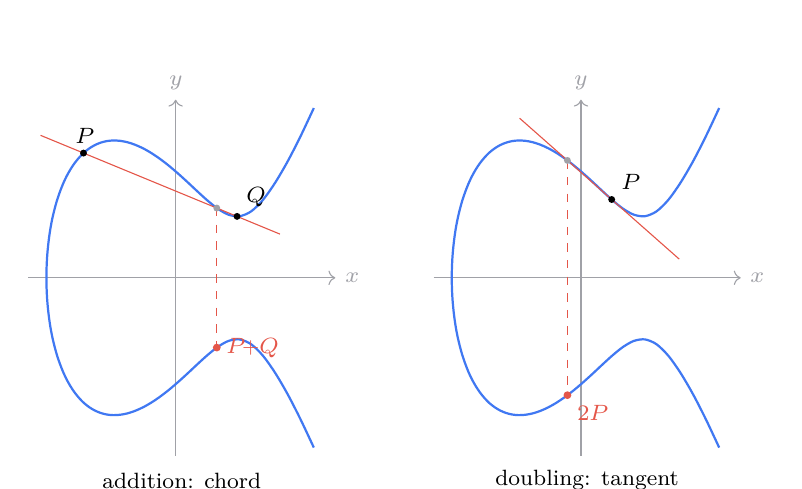
\begin{tikzpicture}[scale=0.78,font=\footnotesize]
\begin{scope}
  \draw[->,gray] (-2.4,0)--(2.6,0) node[right]{$x$}; \draw[->,gray] (0,-2.9)--(0,2.9) node[above]{$y$};
  \draw[acc,thick] plot[smooth] coordinates {(2.250,-2.764) (2.035,-2.307) (1.826,-1.899) (1.621,-1.549) (1.423,-1.270) (1.230,-1.082) (1.042,-1.003) (0.860,-1.028) (0.683,-1.127) (0.511,-1.265) (0.345,-1.416) (0.185,-1.566) (0.030,-1.706) (-0.120,-1.833) (-0.264,-1.943) (-0.403,-2.036) (-0.536,-2.111) (-0.664,-2.168) (-0.787,-2.208) (-0.904,-2.230) (-1.015,-2.236) (-1.121,-2.226) (-1.222,-2.200) (-1.317,-2.160) (-1.407,-2.106) (-1.492,-2.039) (-1.570,-1.959) (-1.644,-1.868) (-1.712,-1.766) (-1.775,-1.654) (-1.832,-1.533) (-1.883,-1.403) (-1.930,-1.266) (-1.970,-1.123) (-2.006,-0.973) (-2.036,-0.819) (-2.060,-0.660) (-2.079,-0.498) (-2.093,-0.333) (-2.101,-0.167) (-2.104,-0.000) (-2.101,0.167) (-2.093,0.333) (-2.079,0.498) (-2.060,0.660) (-2.036,0.819) (-2.006,0.973) (-1.970,1.123) (-1.930,1.266) (-1.883,1.403) (-1.832,1.533) (-1.775,1.654) (-1.712,1.766) (-1.644,1.868) (-1.570,1.959) (-1.492,2.039) (-1.407,2.106) (-1.317,2.160) (-1.222,2.200) (-1.121,2.226) (-1.015,2.236) (-0.904,2.230) (-0.787,2.208) (-0.664,2.168) (-0.536,2.111) (-0.403,2.036) (-0.264,1.943) (-0.120,1.833) (0.030,1.706) (0.185,1.566) (0.345,1.416) (0.511,1.265) (0.683,1.127) (0.860,1.028) (1.042,1.003) (1.230,1.082) (1.423,1.270) (1.621,1.549) (1.826,1.899) (2.035,2.307) (2.250,2.764)};
  \draw[warn] (-2.2,2.320)--(1.7,0.711);
  \draw[warn,dashed] (0.670,1.136)--(0.670,-1.136);
  \fill (-1.5,2.031) circle (1.6pt) node[above]{$P$};
  \fill (1.0,1.0) circle (1.6pt) node[above right]{$Q$};
  \fill[gray] (0.670,1.136) circle (1.6pt);
  \fill[warn] (0.670,-1.136) circle (1.8pt) node[right]{$P{+}Q$};
  \node at (0.1,-3.3) {addition: chord};
\end{scope}
\begin{scope}[xshift=6.6cm]
  \draw[->,gray] (-2.4,0)--(2.6,0) node[right]{$x$}; \draw[->,gray] (0,-2.9)--(0,2.9) node[above]{$y$};
  \draw[acc,thick] plot[smooth] coordinates {(2.250,-2.764) (2.035,-2.307) (1.826,-1.899) (1.621,-1.549) (1.423,-1.270) (1.230,-1.082) (1.042,-1.003) (0.860,-1.028) (0.683,-1.127) (0.511,-1.265) (0.345,-1.416) (0.185,-1.566) (0.030,-1.706) (-0.120,-1.833) (-0.264,-1.943) (-0.403,-2.036) (-0.536,-2.111) (-0.664,-2.168) (-0.787,-2.208) (-0.904,-2.230) (-1.015,-2.236) (-1.121,-2.226) (-1.222,-2.200) (-1.317,-2.160) (-1.407,-2.106) (-1.492,-2.039) (-1.570,-1.959) (-1.644,-1.868) (-1.712,-1.766) (-1.775,-1.654) (-1.832,-1.533) (-1.883,-1.403) (-1.930,-1.266) (-1.970,-1.123) (-2.006,-0.973) (-2.036,-0.819) (-2.060,-0.660) (-2.079,-0.498) (-2.093,-0.333) (-2.101,-0.167) (-2.104,-0.000) (-2.101,0.167) (-2.093,0.333) (-2.079,0.498) (-2.060,0.660) (-2.036,0.819) (-2.006,0.973) (-1.970,1.123) (-1.930,1.266) (-1.883,1.403) (-1.832,1.533) (-1.775,1.654) (-1.712,1.766) (-1.644,1.868) (-1.570,1.959) (-1.492,2.039) (-1.407,2.106) (-1.317,2.160) (-1.222,2.200) (-1.121,2.226) (-1.015,2.236) (-0.904,2.230) (-0.787,2.208) (-0.664,2.168) (-0.536,2.111) (-0.403,2.036) (-0.264,1.943) (-0.120,1.833) (0.030,1.706) (0.185,1.566) (0.345,1.416) (0.511,1.265) (0.683,1.127) (0.860,1.028) (1.042,1.003) (1.230,1.082) (1.423,1.270) (1.621,1.549) (1.826,1.899) (2.035,2.307) (2.250,2.764)};
  \draw[warn] (-1.0,2.599)--(1.6,0.304);
  \draw[warn,dashed] (-0.221,1.911)--(-0.221,-1.911);
  \fill (0.5,1.275) circle (1.6pt) node[above right]{$P$};
  \fill[gray] (-0.221,1.911) circle (1.6pt);
  \fill[warn] (-0.221,-1.911) circle (1.8pt) node[below right]{$2P$};
  \node at (0.1,-3.3) {doubling: tangent};
\end{scope}
\end{tikzpicture}
\end{center}

\textbf{Deriving the formulas.} Let the line through $P = (x_1, y_1)$ have slope $s$: $y = s(x - x_1) + y_1$. Substituting into $y^2 = x^3 + ax + b$ gives a cubic in $x$ whose expanded form starts $x^3 - s^2 x^2 + \dots = 0$. Its three roots are the $x$-coordinates of the three intersection points, and the sum of the roots of a monic cubic is minus the $x^2$ coefficient, so $x_1 + x_2 + x_3 = s^2$, giving $x_3 = s^2 - x_1 - x_2$. The third point is $(x_3,\ s(x_3 - x_1) + y_1)$; reflecting it gives $y_3 = s(x_1 - x_3) - y_1$. For addition, $s$ is the chord slope $(y_2 - y_1)/(x_2 - x_1)$. For doubling, $s$ is the tangent slope: differentiating $y^2 = x^3 + ax + b$ implicitly gives $2y\,y' = 3x^2 + a$, so $s = (3x_1^2 + a)/(2y_1)$, and $x_2 = x_1$. The constant $b$ vanishes on differentiation, which is why the doubling slope contains $a$ and never $b$.

\subsection{Elliptic curves over GF$(p)$ \new}
\likely{Find all the points on $E_{13}(1, 1)$ / $E_{11}(1, 6)$'' and find the inverse of a point'' (3--4 marks).}

Cryptography cannot use real numbers (rounding errors, unbounded size), so the same equation is taken modulo a prime $p > 3$. The curve $E_p(a, b)$ is the set of all pairs $(x, y) \in \mathbb{Z}_p \times \mathbb{Z}_p$ with
\[
y^2 \equiv x^3 + ax + b \pmod p, \qquad a, b \in \mathbb{Z}_p,\quad 4a^3 + 27b^2 \not\equiv 0 \pmod p,
\]
together with the point at infinity $O$. The curve'' is now a finite scatter of points, but the addition formulas derived above still define a group, with every division done as multiplication by an inverse modulo $p$.

\textbf{Finding the points.} For each $x = 0, 1, \dots, p-1$, compute $w = (x^3 + ax + b) \bmod p$, which must equal $y^2$. If $w = 0$ there is one point $(x, 0)$. If $w$ is a nonzero \textbf{quadratic residue} (a perfect square mod $p$), there are two points $(x, \sqrt w)$ and $(x, p - \sqrt w)$. If $w$ is not a square, no point has that $x$. Make the table of squares $y^2 \bmod p$ first; since $(p - y)^2 \equiv y^2$, only $y = 0, \dots, (p-1)/2$ are needed.

\textbf{Negatives.} The inverse of $P = (x, y)$ is $-P = (x, -y) = (x, p - y)$: the same $x$, only $y$ flipped (the reflection in the $x$-axis). A point with $y = 0$ is its own inverse. Points therefore come in vertical pairs $(x, y), (x, p - y)$.

\textbf{Hasse's theorem.} The number of points $\#E$ (including $O$) satisfies $p + 1 - 2\sqrt p \le \#E \le p + 1 + 2\sqrt p$: about half the $x$ values give a square and those give two points each, so \#E is close to $p + 1$. It is a quick check on a point count.

\begin{worked}[: Forouzan/slide, all points of $E_{13}(1, 1)$]
\textbf{Q.} Find all points on $E_{13}(1, 1)$: $y^2 = x^3 + x + 1 \pmod{13}$. List the inverse pairs.

\textbf{Valid curve}: $4 + 27 = 31 \equiv 5 \not\equiv 0 \pmod{13}$. \textbf{Squares mod 13}: $y = 0..6$ give $y^2 = 0, 1, 4, 9, 3, 12, 10$, so the nonzero squares are $\{1, 3, 4, 9, 10, 12\}$ with roots $1 \to \pm1$, $3 \to \pm4$, $4 \to \pm2$, $9 \to \pm3$, $10 \to \pm6$, $12 \to \pm5$.
\begin{center}\small
\begin{tabular}{@{}rrrcl@{}}
\toprule
$x$ & $x^3 + x + 1$ & $w$ & square? & points\\
\midrule
0 & 1 & 1 & yes & (0, 1), (0, 12)\\
1 & 3 & 3 & yes & (1, 4), (1, 9)\\
2 & 11 & 11 & no & --\\
3 & 31 & 5 & no & --\\
4 & 69 & 4 & yes & (4, 2), (4, 11)\\
5 & 131 & 1 & yes & (5, 1), (5, 12)\\
6 & 223 & 2 & no & --\\
7 & 351 & 0 & $y = 0$ & (7, 0)\\
8 & 521 & 1 & yes & (8, 1), (8, 12)\\
9 & 739 & 11 & no & --\\
10 & 1011 & 10 & yes & (10, 6), (10, 7)\\
11 & 1343 & 4 & yes & (11, 2), (11, 11)\\
12 & 1741 & 12 & yes & (12, 5), (12, 8)\\
\bottomrule
\end{tabular}
\end{center}
\textbf{17 points + $O$ = 18.} Each row's two points are inverses (e.g.\ $4 + 9 = 13$, so $(1, 9) = -(1, 4)$); $(7, 0)$ is its own inverse. $x = 2, 3, 6, 9$ give non-squares. Hasse: $14 \pm 2\sqrt{13} = [6.8,\ 21.2]$ contains 18 \checkmark.
\end{worked}

\begin{worked}[: new, all points of $E_{11}(1, 6)$]
\textbf{Q.} Find all points on $y^2 = x^3 + x + 6 \pmod{11}$ and verify Hasse's bound.

\textbf{Valid}: $4 + 27 \cdot 36 = 976 = 88 \cdot 11 + 8 \not\equiv 0$. \textbf{Squares mod 11}: $y = 0..5$ give $0, 1, 4, 9, 5, 3$; nonzero squares $\{1, 3, 4, 5, 9\}$ with roots $1 \to \pm1$, $3 \to \pm5$, $4 \to \pm2$, $5 \to \pm4$, $9 \to \pm3$.
\begin{center}\small
\begin{tabular}{@{}rrrcl@{\qquad}rrrcl@{}}
\toprule
$x$ & $x^3{+}x{+}6$ & $w$ & sq? & points & $x$ & $x^3{+}x{+}6$ & $w$ & sq? & points\\
\midrule
0 & 6 & 6 & no & -- & 6 & 228 & 8 & no & --\\
1 & 8 & 8 & no & -- & 7 & 356 & 4 & yes & (7, 2), (7, 9)\\
2 & 16 & 5 & yes & (2, 4), (2, 7) & 8 & 526 & 9 & yes & (8, 3), (8, 8)\\
3 & 36 & 3 & yes & (3, 5), (3, 6) & 9 & 744 & 7 & no & --\\
4 & 74 & 8 & no & -- & 10 & 1016 & 4 & yes & (10, 2), (10, 9)\\
5 & 136 & 4 & yes & (5, 2), (5, 9) & & & & & \\
\bottomrule
\end{tabular}
\end{center}
\textbf{12 points + $O$ = 13.} Hasse: $12 \pm 2\sqrt{11} = [5.4,\ 18.6]$ contains 13 \checkmark. Since 13 is prime, every point except $O$ generates the whole group (Lagrange).
\end{worked}

\subsection{Point addition and doubling over GF$(p)$ \new}
\likely{``Add $P$ and $Q$ / find $2P$ on $E_p(a, b)$'' (2--3 marks), always with modular inverses.}

\begin{mustknow}[: EC group law over GF$(p)$]
For $P = (x_1, y_1)$, $Q = (x_2, y_2)$, \;$R = P + Q = (x_3, y_3)$ with
\[
x_3 = s^2 - x_1 - x_2 \bmod p, \qquad y_3 = s(x_1 - x_3) - y_1 \bmod p,
\]
\[
s = \frac{y_2 - y_1}{x_2 - x_1} \bmod p \ \ (P \ne Q,\ \text{addition}), \qquad s = \frac{3x_1^2 + a}{2y_1} \bmod p \ \ (P = Q,\ \text{doubling}).
\]
Division means multiplying by the inverse mod $p$. Special cases: $P + O = P$; if $x_1 = x_2$ and $y_2 = -y_1$ then $P + Q = O$; doubling a point with $y_1 = 0$ gives $O$.
\end{mustknow}

\begin{worked}[: one addition and two doublings]
\textbf{Q1 (Forouzan style).} On $E_{13}(1, 1)$, add $P = (4, 2)$ and $Q = (10, 6)$.\\
$s = (6 - 2)(10 - 4)^{-1} = 4 \cdot 6^{-1} = 4 \cdot 11 = 44 \equiv 5$ \;($6 \cdot 11 = 66 = 5 \cdot 13 + 1$).\\
$x_3 = 25 - 4 - 10 = 11$; \;$y_3 = 5(4 - 11) - 2 = -37 \equiv -37 + 39 = 2$. \;$\mathbf{P + Q = (11, 2)}$, which is in the point list \checkmark.

\textbf{Q2.} On $E_{13}(1, 1)$, find $2P$ for $P = (1, 4)$.\\
$s = (3 \cdot 1^2 + 1)(2 \cdot 4)^{-1} = 4 \cdot 8^{-1} = 4 \cdot 5 = 20 \equiv 7$ \;($8 \cdot 5 = 40 = 3 \cdot 13 + 1$).\\
$x_3 = 49 - 1 - 1 = 47 \equiv 8$; \;$y_3 = 7(1 - 8) - 4 = -53 \equiv -53 + 65 = 12$. \;$\mathbf{2P = (8, 12)}$ \checkmark.

\textbf{Q3 (slide).} On $E_{17}(2, 2)$: $y^2 = x^3 + 2x + 2$, find $2P$ for $P = (5, 1)$.\\
$s = (3 \cdot 5^2 + 2)(2 \cdot 1)^{-1} = 77 \cdot 2^{-1} \equiv 9 \cdot 9 = 81 \equiv 13$ \;($77 = 4 \cdot 17 + 9$, $2^{-1} = 9$).\\
$x_3 = 169 - 5 - 5 = 159 = 9 \cdot 17 + 6 \equiv 6$; \;$y_3 = 13(5 - 6) - 1 = -14 \equiv 3$. \;$\mathbf{2P = (6, 3)}$.\\
Check: $3^2 = 9$ and $6^3 + 2 \cdot 6 + 2 = 230 = 13 \cdot 17 + 9$ \checkmark. (This curve has 19 points and $(5, 1)$ generates all of them.)
\end{worked}

\begin{trap}[: point arithmetic slips]
The doubling slope uses $a$ (from $3x^2 + a$), never $b$. Compute $s$ as an integer mod $p$ with a modular inverse, never as a fraction or decimal. $-P = (x, p - y)$ flips only $y$. Use the addition formula only for $P \ne Q$ (it would divide by $x_2 - x_1 = 0$). Reduce negative results by adding multiples of $p$, and check the answer lies on the curve.
\end{trap}

\subsection{Scalar multiplication and the ECDLP \new}
\likely{``Compute $kP$ for small $k$ and ``state the ECDLP / Hasse's theorem.}
Multiplying a point by an integer $k$ means adding it to itself: $kP = P + P + \dots + P$ ($k$ times). It is computed by \textbf{double-and-add}, the analogue of square-and-multiply: scan the bits of $k$, double at every bit and add $P$ at every 1-bit, so $kP$ costs about $\log_2 k$ doublings. The slides' two examples on $E_{13}(1, 1)$, recomputed:
\begin{itemize}[leftmargin=1.4em]
  \item $4 \cdot (1, 4) = 2 \cdot (2 \cdot (1, 4)) = 2 \cdot (8, 12)$: $s = (3 \cdot 64 + 1) \cdot 24^{-1} \equiv 11 \cdot 11^{-1} = 1$, $x_3 = 1 - 16 \equiv 11$, $y_3 = 1 \cdot (8 - 11) - 12 = -15 \equiv 11$, so $4 \cdot (1, 4) = \mathbf{(11, 11)}$ \checkmark.
  \item $3 \cdot (8, 1) = 2 \cdot (8, 1) + (8, 1)$: doubling gives $s = 193 \cdot 2^{-1} \equiv 11 \cdot 7 \equiv 12$, $(11, 2)$; then $(11, 2) + (8, 1)$: $s = (-1)(-3)^{-1} \equiv 12 \cdot 10^{-1} = 12 \cdot 4 \equiv 9$, $x_3 = 81 - 19 \equiv 10$, $y_3 = 9(11 - 10) - 2 = 7$, so $3 \cdot (8, 1) = \mathbf{(10, 7)}$ \checkmark.
\end{itemize}
$(1, 4)$ has order 18, so it generates all of $E_{13}(1, 1)$; its multiples (useful for checking the examples below) are:
\begin{center}\small
\begin{tabular}{@{}c|ccccccccc@{}}
\toprule
$k$ & 1 & 2 & 3 & 4 & 5 & 6 & 7 & 8 & 9\\
$k(1,4)$ & (1,4) & (8,12) & (0,12) & (11,11) & (5,1) & (10,6) & (12,8) & (4,2) & (7,0)\\
\midrule
$k$ & 17 & 16 & 15 & 14 & 13 & 12 & 11 & 10 & 18\\
$k(1,4)$ & (1,9) & (8,1) & (0,1) & (11,2) & (5,12) & (10,7) & (12,5) & (4,11) & $O$\\
\bottomrule
\end{tabular}
\end{center}
The second row is the negative of the first ($(18 - k)P = -kP$), and $9P = (7, 0)$ has $y = 0$, so $18P = 2 \cdot 9P = O$.

\textbf{Elliptic curve discrete logarithm problem (ECDLP).} Given a point $P$ (ideally a generator) and $T = dP$, find $d$ with $1 \le d \le \#E$. Computing $T$ from $d$ takes about $\log_2 d$ doublings, but no shortcut is known for the reverse: on a well-chosen curve the best attack is a generic one such as \textbf{Pollard's rho}, which needs about $\sqrt{\#E}$ steps. On the toy curve the table answers it at once ($T = (4, 2) \Rightarrow d = 8$); for a 160-bit curve, $\sqrt{\#E} \approx 2^{80}$ steps is infeasible.

\subsection{ECC simulating ElGamal \new}
\likely{``Explain ECC encryption/decryption; verify the given example'' (the slide's $E_{67}(2, 3)$ example).}

ElGamal works in any group where the discrete log is hard, so it carries over by a dictionary: multiplication mod $p$ becomes point addition, exponentiation becomes scalar multiplication, and the inverse becomes the negative point. The plaintext must be encoded as a point $P$ on the curve.

\begin{mustknow}[: EC ElGamal]
\textbf{Keys (Bob)}: choose $E_p(a, b)$, a point $e_1$ on it, and an integer $d$; compute $e_2 = d \times e_1$. Public $(E_p(a, b), e_1, e_2)$, private $d$.\\
\textbf{Encrypt (Alice)}: fresh random $r$; \;$C_1 = r \times e_1$, \;$C_2 = P + r \times e_2$.\\
\textbf{Decrypt (Bob)}: $P = C_2 - (d \times C_1)$, where subtracting means adding the negative point.\\
Proof: $C_2 - d C_1 = P + r(d e_1) - d(r e_1) = P + (rd) e_1 - (dr) e_1 = P + O = P$.
\end{mustknow}

\begin{worked}[: the slide example on $E_{67}(2, 3)$, every step]
\textbf{Q.} Bob selects $E_{67}(2, 3)$, $e_1 = (2, 22)$, $d = 4$. Alice sends $P = (24, 26)$ with $r = 2$. Find $e_2$, $C_1$, $C_2$, and verify decryption.

\begin{center}\small
\begin{tabular}{@{}lllll@{}}
\toprule
Step & Slope $s$ (mod 67) & $x_3$ & $y_3$ & Result\\
\midrule
$2e_1 = 2(2, 22)$ & $14 \cdot 44^{-1} = 14 \cdot 32 \equiv 46$ & $2112 \equiv 35$ & $-1540 \equiv 1$ & $(35, 1)$\\
$4e_1 = 2(35, 1)$ & $3677 \cdot 2^{-1} \equiv 59 \cdot 34 \equiv 63$ & $3899 \equiv 13$ & $1385 \equiv 45$ & $(13, 45)$\\
$2e_2 = 2(13, 45)$ & $509 \cdot 90^{-1} \equiv 40 \cdot 35 \equiv 60$ & $3574 \equiv 23$ & $-645 \equiv 25$ & $(23, 25)$\\
$P + 2e_2$ & $(-1)(-1)^{-1} = 1$ & $-46 \equiv 21$ & $-23 \equiv 44$ & $(21, 44)$\\
$C_2 + (23, 42)$ & $(-2) \cdot 2^{-1} \equiv 66$ & $4312 \equiv 24$ & $-242 \equiv 26$ & $(24, 26)$\\
\bottomrule
\end{tabular}
\end{center}
\textbf{Keys}: $e_2 = 4 e_1 = (13, 45)$. \textbf{Encrypt}: $C_1 = 2 e_1 = (35, 1)$, $r e_2 = (23, 25)$, $C_2 = (24, 26) + (23, 25) = (21, 44)$.\\
\textbf{Decrypt}: $d \times C_1 = 4 \cdot (35, 1) = 8 e_1 = 2 e_2 = (23, 25)$ (two doublings, rows 2--3). Its negative is $(23, 67 - 25) = (23, 42)$, and $(21, 44) + (23, 42) = \mathbf{(24, 26)} = P$ \checkmark.\\
Inverses used: $44 \cdot 32 = 1408 = 21 \cdot 67 + 1$; $2 \cdot 34 = 68$; $23 \cdot 35 = 805 = 12 \cdot 67 + 1$ ($90 \equiv 23$).
\end{worked}

\begin{worked}[: new exam-style example on $E_{13}(1, 1)$]
\textbf{Q.} Bob uses $E_{13}(1, 1)$ with $e_1 = (1, 4)$ and private key $d = 3$. Alice encrypts the point $P = (4, 2)$ with $r = 2$. Find Bob's public key, the ciphertext, and verify decryption.

\begin{center}\small
\begin{tabular}{@{}lllll@{}}
\toprule
Step & Slope $s$ (mod 13) & $x_3$ & $y_3$ & Result\\
\midrule
$2e_1 = 2(1, 4)$ & $4 \cdot 8^{-1} = 4 \cdot 5 \equiv 7$ & $47 \equiv 8$ & $-53 \equiv 12$ & $(8, 12)$\\
$e_2 = (8, 12) + (1, 4)$ & $(-8)(-7)^{-1} = 5 \cdot 6^{-1} = 5 \cdot 11 \equiv 3$ & $0$ & $12$ & $(0, 12)$\\
$2e_2 = 2(0, 12)$ & $1 \cdot 24^{-1} = 11^{-1} = 6$ & $36 \equiv 10$ & $-72 \equiv 6$ & $(10, 6)$\\
$C_2 = (4, 2) + (10, 6)$ & $4 \cdot 6^{-1} \equiv 5$ & $11$ & $-37 \equiv 2$ & $(11, 2)$\\
$2C_1 = 2(8, 12)$ & $193 \cdot 24^{-1} \equiv 11 \cdot 6 \equiv 1$ & $-15 \equiv 11$ & $-15 \equiv 11$ & $(11, 11)$\\
$3C_1 = (11, 11) + (8, 12)$ & $1 \cdot (-3)^{-1} = 10^{-1} = 4$ & $-3 \equiv 10$ & $-7 \equiv 6$ & $(10, 6)$\\
$C_2 + (10, 7)$ & $5 \cdot (-1)^{-1} = 5 \cdot 12 \equiv 8$ & $43 \equiv 4$ & $54 \equiv 2$ & $(4, 2)$\\
\bottomrule
\end{tabular}
\end{center}
\textbf{Public key} $(E_{13}(1, 1), (1, 4), (0, 12))$. \textbf{Ciphertext} $C_1 = 2 e_1 = \mathbf{(8, 12)}$, $C_2 = \mathbf{(11, 2)}$.\\
\textbf{Decrypt}: $d \times C_1 = 3 \cdot (8, 12) = (10, 6)$, the same point as $r \times e_2$; negative $(10, 7)$; $(11, 2) + (10, 7) = \mathbf{(4, 2)}$ \checkmark. In multiples of $e_1$ (table above): $e_2 = 3e_1$, $C_1 = 2e_1$, $P = 8e_1$, $C_2 = (8 + 6)e_1 = 14 e_1$, and $14 - 6 = 8$ \checkmark.
\end{worked}

\subsection{Security of ECC and key size \new}
\likely{``Why does ECC need smaller keys than RSA for the same security? (2 marks).}
To decrypt, Eve needs $r$ (then $P = C_2 - r \times e_2$) or $d$ (then $P = C_2 - d \times C_1$). Finding $r$ from $C_1 = r \times e_1$, or $d$ from $e_2 = d \times e_1$, is the ECDLP, which for large $p$ (or large $n$ in GF$(2^n)$) is infeasible by Pollard's rho. As in ElGamal, $r$ must be fresh for every message.

\textbf{Why ECC keys are smaller.} For factoring and for the discrete log in $\mathbb{Z}_p^*$ there are \textbf{sub-exponential} algorithms (the number field sieve, index calculus) that exploit the arithmetic structure of integers, so RSA and ElGamal need 1024-bit and larger moduli to stay ahead. On a well-chosen elliptic curve no such structure is known, and only generic attacks costing about $\sqrt{\#E}$ work, i.e.\ $2^{k/2}$ for a $k$-bit curve. A 160-bit curve therefore costs about $2^{80}$ steps, the same effort as factoring a 1024-bit RSA modulus: \imp{ECC over GF$(2^n)$ or GF$(p)$ with a 160-bit modulus gives the same security as RSA with a 1024-bit modulus} (and 256-bit ECC $\approx$ 3072-bit RSA). Smaller keys mean less computation, bandwidth and storage, which suits smart cards and mobile devices.


\begin{fixbox}
\begin{itemize}[leftmargin=1.2em,itemsep=0pt]
  \item ElGamal block diagram: the encryption box labels both lines $C_1$; the second line, $(e_2^r \cdot P) \bmod p$, is $\boldsymbol{C_2}$.
  \item $E_{67}(2, 3)$ example, step 8: ``He uses $2 \times C_1$'' should read $d \times C_1 = \boldsymbol{4} \times C_1 = (23, 25)$. With $C_1 = 2e_1$, $2 \times C_1 = 4e_1 = e_2 = (13, 45)$, not $(23, 25)$ (recomputed). The same misprint is in Forouzan.
  \item ElGamal security slide: 1024 bits is about \textbf{309} decimal digits (as on the RSA slide), not 300.
\end{itemize}
\end{fixbox}

% College Lecture 14: message integrity, birthday problems, hash attacks, iterated hashes, SHA-512, Whirlpool.
% Sources: slides L14 (58 slides), Forouzan ch. 11 + 12. Every number recomputed by script (scratchpad/hash/verify*.py).
\section{Message Integrity and Hash Functions}\label{sec:integrity}
\usetikzlibrary{decorations.pathreplacing}

\subsection{Integrity versus secrecy; message and digest \new}
\likely{``Why is a hash, not encryption, used for integrity?'' and ``how is integrity checked with a digest?'' (2--3 marks).}

Every scheme so far gave \emph{secrecy}: Eve cannot read the message. Many documents need the opposite guarantee. Alice's will, for example, need not be encrypted, because after her death anyone may read it; what must be preserved is its \emph{integrity}, meaning that nobody can change its contents without the change being noticed. On paper this is achieved by putting Alice's fingerprint at the bottom of the document: Eve can read the will, but she cannot alter it or write a false one, because she cannot forge the fingerprint.

The electronic equivalent of the document--fingerprint pair is the \textbf{message--digest pair}. The message is passed through a \textbf{cryptographic hash function} $h$, which maps a message of any length to a short fixed-length string $h(M)$, called the \textbf{message digest}. The digest is a compressed image of the message that plays the role of the fingerprint. To check integrity later, the receiver runs the same hash function on the message he now holds and compares the new digest with the stored one: \imp{if the two digests are equal, the message has not been changed; if they differ, the message was changed and is discarded.}

\textbf{Why a hash and not encryption.} Encryption hides the message but does not stop Eve from altering the ciphertext; flipping a bit of a one-time-pad or stream-cipher ciphertext flips the same bit of the plaintext, and Bob has no way to tell a changed plaintext from a genuine one. A hash works the other way round: it hides nothing (the message can be public), but since any change to the message produces a different digest, any change is detected. The two services are therefore independent, and a message can need one, the other, or both.

\textbf{The digest itself must be safe.} The check only works if the stored or received digest is genuine. If Eve can replace both $M$ and $h(M)$, she simply sends $M'$ with $h(M')$ and the comparison passes. Hence the digest is kept in a safe place or sent over an authenticated channel; binding the digest to a secret key gives the MAC of the next lecture.

\subsection{The three security criteria \new}
\likely{``Define and differentiate preimage, second preimage and collision resistance'' (3--4 marks), possibly with a figure of what Eve is given and must find.}

A cryptographic hash function must make three kinds of forgery infeasible. They differ in how much Eve is given at the start, and therefore in how much freedom she has.

\textbf{Preimage resistance.} Given a hash function $h$ and a digest $y = h(M)$, it must be extremely difficult for Eve to find \emph{any} message $M'$ with $h(M') = y$. If $h$ were not preimage resistant, Eve could intercept just the digest $h(M)$, construct a message $M'$ that hashes to it, and send $M'$ to Bob as if it were $M$. In other words, the hash must be one-way.

\textbf{Second preimage resistance.} Given a specific message $M$ \emph{and} its digest $h(M)$, it must be extremely difficult to find another message $M' \ne M$ with $h(M') = h(M)$. This is the criterion that stops forgery of a particular message: if Alice sends $M$ and $h(M)$ to Bob, Eve cannot create a different message with the same digest and substitute it. Eve here has more information than in the preimage case (she also knows one valid preimage), but she still has to hit one fixed target value.

\textbf{Collision resistance.} It must be extremely difficult to find \emph{any} two messages $M \ne M'$ with $h(M) = h(M')$. Here Eve is given nothing and is free to choose both messages from scratch; such a pair is called a \textbf{collision}. This is the danger when Eve prepares two documents herself (say a fair contract and an unfair one with the same digest), gets Alice to approve the fair one, and later swaps in the other.

\begin{center}\small
\begin{tabularx}{\textwidth}{@{}l X X l@{}}
\toprule
Criterion & Eve is given & Eve must find & Attack it stops\\
\midrule
Preimage resistance & $h$ and a digest $y = h(M)$ & any $M'$ with $h(M') = y$ & preimage\\
Second preimage resistance & $h$, a message $M$ and $h(M)$ & $M' \ne M$ with $h(M') = h(M)$ & second preimage\\
Collision resistance & only $h$ & any pair $M \ne M'$ with $h(M) = h(M')$ & collision\\
\bottomrule
\end{tabularx}
\end{center}

\textbf{Collision resistance implies second preimage resistance.} Suppose Eve had a method that, given any $M$, produces a second preimage $M'$. She could then pick any $M$ she likes, run the method, and output the pair $(M, M')$, which is a collision. So a function that is \emph{not} second-preimage resistant cannot be collision resistant; equivalently, a collision-resistant function is automatically second-preimage resistant. The converse fails, because finding a collision is the easier task (Eve chooses both sides), and the birthday analysis below shows by how much: a collision costs about $2^{n/2}$ hash evaluations, a second preimage about $2^n$.

\textbf{Why a compressor or a checksum is not a cryptographic hash.} A lossless compression method such as ZIP or StuffIt also shrinks the message, but it is reversible: anyone can decompress the output and get the original, so it is not even a function to a fixed-length output, and it fails preimage resistance trivially. A checksum (adding up the bytes, a CRC) is fixed-length but linear and easy to invert: given a target checksum, Eve can compute what to change in any message to reach it, so it is neither preimage nor second-preimage resistant. Checksums detect accidental errors, not deliberate ones.

\begin{mustknow}[: the three criteria]
\textbf{Preimage}: given $y$, find any $M'$ with $h(M') = y$. \quad \textbf{Second preimage}: given $M$, find $M' \ne M$ with $h(M') = h(M)$. \quad \textbf{Collision}: find any $M \ne M'$ with $h(M) = h(M')$.\\
Cost for an ideal $n$-bit hash: preimage and second preimage $\approx 2^n$, collision $\approx 2^{n/2}$. Collision resistance $\Rightarrow$ second preimage resistance.
\end{mustknow}

\subsection{The random oracle model \new}
\likely{``Explain the random oracle model; why can the oracle not use a formula?'' (2--3 marks).}

To analyse attacks we need a model of a perfect hash function, against which real designs are compared. The \textbf{random oracle model} (Bellare and Rogaway, 1993) describes such an ideal function as an oracle that keeps a table of the messages it has already hashed and obeys three rules:
\begin{enumerate}[nosep]
  \item When a \emph{new} message of any length is given, the oracle creates a fixed-length digest that is a truly random string of 0s and 1s, gives it out, and records the message and digest in its table.
  \item When a message is given for which a digest already exists, the oracle simply returns the digest in the table. This makes the function deterministic: the same message always gets the same digest.
  \item The digest for a new message must be chosen independently of all previous digests. This implies that the oracle cannot use a formula or an algorithm to calculate the digest.
\end{enumerate}

\textbf{Example (slides 20--23).} An oracle with 16-bit digests already holds three entries. It is asked to hash \ttx{AB1234CD8765BDAD}, which is not in its table, so it flips a fair coin 16 times and gets \ttx{HHTHHHTTHTHHTTTH}. Reading H as 1 and T as 0 gives \ttx{1101 1100 1011 0001} $=$ \ttx{DCB1}, which it returns and records. When it is then asked for \ttx{4523AB1352CDEF45126}, which is already in the table, it does not flip again but returns the stored digest \ttx{13AB}.
\begin{center}\small
\begin{tabular}{@{}ll@{}}
\toprule
Message & Digest\\
\midrule
\ttx{4523AB1352CDEF45126} & \ttx{13AB}\\
\ttx{723BAE38F2AB3457AC} & \ttx{02CA}\\
\ttx{AB1234CD8765BDAD} & \ttx{DCB1} (new)\\
\ttx{AB45CD1048765412AAAB6662BE} & \ttx{A38B}\\
\bottomrule
\end{tabular}
\end{center}

\textbf{Why a formula violates rule 3.} Suppose the oracle used $h(M) = M \bmod n$ and had already issued $h(M_1)$ and $h(M_2)$. For the new message $M_3 = M_1 + M_2$ anyone can predict the digest without asking, since
\[
h(M_3) = (M_1 + M_2) \bmod n = [\,h(M_1) + h(M_2)\,] \bmod n .
\]
The digest of $M_3$ is therefore not independent of the earlier digests, which breaks rule 3. Real hash functions are algorithms, so they can only approximate the oracle; the model tells us the best security an $n$-bit design can hope for.

\textbf{What the model gives an attacker.} With an $n$-bit digest there are $N = 2^n$ possible digests, and each new message receives one of them uniformly at random. Some values may be chosen several times and some never. Eve knows the algorithm and $n$, so every attack reduces to drawing random digests and waiting for a match, which is exactly a birthday problem.

\subsection{The four birthday problems \new}
\likely{Derive the probability formula for one problem and get $k$ for $P = 1/2$; or ``how many people for a shared birthday'' (23).}

All four problems use a random variable that is uniform over $N$ values ($0$ to $N - 1$; $N = 365$ for birthdays) and ask for the minimum number of samples $k$ that makes an event \emph{likely}, meaning probability $P \ge 1/2$. Every derivation uses the approximation $1 - x \approx e^{-x}$ for small $x$.

\textbf{Problem 1: a sample equals a predefined value.} What is the minimum number of students such that it is likely that at least one has a \emph{predefined} birthday (say 1 January)? A single sample misses the target with probability $1 - 1/N$, and the $k$ samples are independent, so all of them miss with probability $(1 - 1/N)^k \approx e^{-k/N}$. Hence
\[
P_1 \approx 1 - e^{-k/N}, \qquad k \approx \ln\frac{1}{1-P}\times N \;\xrightarrow{P = 1/2}\; k \approx \ln 2 \times N = 0.69N .
\]
For $N = 365$: $0.693 \times 365 = 252.99$, so $k = 253$.

\textbf{Problem 2: a sample equals one chosen from the set.} What is the minimum number such that it is likely that at least one student has the same birthday as a student \emph{selected by the professor}? The selected student is one of the $k$, so only the other $k - 1$ can match, and the problem is Problem 1 with $k - 1$ samples:
\[
P_2 \approx 1 - e^{-(k-1)/N}, \qquad k \approx \ln 2 \times N + 1 = 0.69N + 1 ;\qquad N = 365:\ k = 254 .
\]

\textbf{Problem 3: any two samples are equal (the birthday paradox).} What is the minimum number such that it is likely that \emph{at least two} students share a birthday? It is easier to count the complement, that all $k$ values are different. The first value is free, the second must avoid 1 value, the $i$-th must avoid $i - 1$ values, so
\[
\Pr[\text{all different}] = \prod_{i=1}^{k-1}\Bigl(1 - \frac{i}{N}\Bigr) \approx \prod_{i=1}^{k-1} e^{-i/N} = e^{-(1 + 2 + \dots + (k-1))/N} = e^{-k(k-1)/2N}.
\]
Therefore
\[
P_3 \approx 1 - e^{-k(k-1)/2N}, \qquad k \approx \Bigl\{2\ln\frac{1}{1-P}\Bigr\}^{1/2} N^{1/2} \;\xrightarrow{P = 1/2}\; k \approx \sqrt{2\ln 2}\,\sqrt N = 1.18\sqrt N ,
\]
using $k(k-1) \approx k^2$. For $N = 365$: $1.18 \times 19.1 = 22.5$, so $k = 23$ (exactly, 23 people give $P = 0.507$ and 22 give $0.476$). The answer is a ``paradox'' only because intuition compares each person with \emph{one} date, whereas $k$ people form $k(k-1)/2 = 253$ pairs, each a chance to match.

\textbf{Problem 4: a sample of one set equals a sample of another.} Two classes each have $k$ students. What is the minimum $k$ such that it is likely that some student of the first class shares a birthday with some student of the second? Treat the $k$ values of set 1 as (nearly) distinct. Each value of set 2 then misses all of them with probability $1 - k/N$, and the $k$ values of set 2 all miss with probability $(1 - k/N)^k \approx e^{-k^2/N}$. Hence
\[
P_4 \approx 1 - e^{-k^2/N}, \qquad k \approx \Bigl\{\ln\frac{1}{1-P}\Bigr\}^{1/2} N^{1/2} \;\xrightarrow{P = 1/2}\; k \approx \sqrt{\ln 2}\,\sqrt N = 0.83\sqrt N ;\qquad N = 365:\ k = 16 .
\]
(Exactly, $k = 16$ gives $P = 0.504$.)

\begin{center}\small
\begin{tabular}{@{}clllcl@{}}
\toprule
Problem & Probability $P$ & General $k$ & $k$ at $P = \tfrac12$ & $N = 365$ & Attack\\
\midrule
1 & $1 - e^{-k/N}$ & $\ln\frac{1}{1-P} \cdot N$ & $0.69N$ & 253 & preimage\\
2 & $1 - e^{-(k-1)/N}$ & $\ln\frac{1}{1-P} \cdot N + 1$ & $0.69N + 1$ & 254 & second preimage\\
3 & $1 - e^{-k(k-1)/2N}$ & $\{2\ln\frac{1}{1-P}\}^{1/2} N^{1/2}$ & $1.18\sqrt N$ & 23 & collision\\
4 & $1 - e^{-k^2/N}$ & $\{\ln\frac{1}{1-P}\}^{1/2} N^{1/2}$ & $0.83\sqrt N$ & 16 & alternate collision\\
\bottomrule
\end{tabular}
\end{center}
The constants are $0.69 = \ln 2$, $1.18 = \sqrt{2\ln 2}$ and $0.83 = \sqrt{\ln 2}$. The key comparison is that \textbf{$k$ grows like $N$ in Problems 1 and 2 but only like $\sqrt N$ in Problems 3 and 4}. Problems 1 and 2 model the preimage and second preimage attacks, Problems 3 and 4 the collision attacks, so a collision attack is far cheaper than a preimage attack on the same hash.

\begin{trap}[: rounding the constant]
With $0.69$ exactly, $0.69 \times 365 = 251.85$, which would suggest 252; the table value 253 comes from $\ln 2 = 0.6931$ ($0.6931 \times 365 = 252.99$). Use $0.693$ when the answer must be an exact head count. Also do not mix up Problems 1 and 3: ``someone has \emph{my} birthday'' needs 253 people, ``\emph{some two} share a birthday'' needs only 23.
\end{trap}

\begin{worked}[: birthday numbers for a 16-bit digest]
\textbf{Q.} A hash function produces 16-bit digests. Using the birthday results, how many random messages must Eve hash for a probability of at least $1/2$ of (a) matching a given digest, (b) finding any two messages with the same digest, (c) a match between two lists of $k$ messages each?

\textbf{A.} $N = 2^{16} = 65\,536$ and $\sqrt N = 2^8 = 256$.\\
(a) Problem 1: $k \approx 0.69 \times 65\,536 \approx 45\,220$ messages (order $2^{16}$).\\
(b) Problem 3: $k \approx 1.18 \times 256 \approx \mathbf{302}$ messages (order $2^8$).\\
(c) Problem 4: $k \approx 0.83 \times 256 \approx \mathbf{213}$ messages in each list.\\
\emph{Check}: (b) is about 150 times cheaper than (a), as $2^{16}/2^8 = 256$ predicts up to the constants.
\end{worked}

\subsection{Attacks on an $n$-bit digest \new}
\likely{``A hash uses a 64-bit digest; how many digests must Eve create to find a collision (or the original message) with $P > 0.5$, and how long does it take?'' (3--4 marks).}

Assume the hash behaves like a random oracle with $n$-bit digests, so its outputs are uniform over $N = 2^n$ values, and that Eve knows the algorithm and $n$. Each attack below is a loop that creates messages, hashes them, and compares digests; its success probability is the matching birthday problem.

\textbf{Preimage attack.} Eve has intercepted a digest $D = h(M)$ and wants any $M'$ with $h(M') = D$. She creates $k$ messages $M[1], \dots, M[k]$, computes $T = h(M[i])$ for each, and returns $M[i]$ as soon as $T = D$. The target $D$ is a predefined value, so this is Problem 1: $P = 1 - e^{-k/N}$, and success with $P \ge 1/2$ needs $k = 0.69 \times 2^n$ digests, which is of order $2^n$.

\textbf{Second preimage attack.} Eve has intercepted both $M$ and $D = h(M)$ and wants $M' \ne M$ with $h(M') = D$. She creates $k - 1$ further messages and compares each digest with $D$. The target is one of the $k$ samples (the given $M$), so this is Problem 2: $P = 1 - e^{-(k-1)/N}$ and $k = 0.69 \times 2^n + 1$, again of order $2^n$.

\textbf{Collision attack.} Eve wants any $M \ne M'$ with $h(M) = h(M')$. She creates $k$ messages, stores the digests $D[1], \dots, D[k]$, and compares each new digest with all earlier ones. Any two equal digests suffice, so this is Problem 3: $P = 1 - e^{-k(k-1)/2N}$ and $k = 1.18 \times 2^{n/2}$, of order only $2^{n/2}$. The square root comes from the number of pairs: $k$ digests give about $k^2/2$ pairs, and once $k^2/2$ is comparable to $2^n$ a coincidence is likely.

\textbf{Alternate collision attack.} A random collision is usually useless, because the two colliding messages are meaningless strings. A real forger needs a collision between a \emph{genuine} message $M$ (which Alice will approve) and a \emph{bogus} message $M'$ (which Eve will later substitute), both meaningful. Eve therefore makes $k$ variants of each without changing their meaning (an extra space after a word, a synonym, ``will not'' versus ``won't'', a redundant phrase): $M_1, \dots, M_k$ and $M'_1, \dots, M'_k$. She hashes both lists and looks for $h(M_i) = h(M'_j)$. A match must be \emph{across} the two lists, so this is Problem 4: $P = 1 - e^{-k^2/N}$ and $k = 0.83 \times 2^{n/2}$ variants of each, still of order $2^{n/2}$. Variants are cheap to produce: if a letter has $n/2$ independent places where one of two equivalent forms can be used, it has $2^{n/2}$ variants.

\begin{center}\small
\begin{tabular}{@{}llll@{}}
\toprule
Attack & Birthday problem & $k$ for $P = 1/2$ & Order\\
\midrule
Preimage & 1 & $0.69 \times 2^n$ & $2^n$\\
Second preimage & 2 & $0.69 \times 2^n + 1$ & $2^n$\\
Collision & 3 & $1.18 \times 2^{n/2}$ & $2^{n/2}$\\
Alternate collision & 4 & $0.83 \times 2^{n/2}$ & $2^{n/2}$\\
\bottomrule
\end{tabular}
\end{center}

\begin{worked}[: a 64-bit digest (slides 27 and 32)]
\textbf{Q.} A cryptographic hash function uses a 64-bit digest. (a) How many digests must Eve create to find the original message with probability more than $0.5$, and how long does it take at $2^{30}$ (about one billion) digests per second? (b) How many digests must she create to find two messages with the same digest with probability more than $0.5$, and how long does it take at $2^{20}$ (about one million) digests per second? Is a 64-bit digest secure?

\textbf{A.} $n = 64$, $N = 2^{64}$.\\
(a) Preimage attack (Problem 1): $k = 0.69 \times 2^{64} \approx 1.27 \times 10^{19}$ digests.\\
Time $= 0.69 \times 2^{64} / 2^{30} = 0.69 \times 2^{34}$ s $= 1.185 \times 10^{10}$ s $\div (3.156 \times 10^{7}$ s/year$) \approx \mathbf{376}$ \textbf{years}. Secure against the preimage attack.\\
(b) Collision attack (Problem 3): $k = 1.18 \times 2^{64/2} = 1.18 \times 2^{32} \approx 5.07 \times 10^{9}$ digests.\\
Time $= 1.18 \times 2^{32} / 2^{20} = 1.18 \times 2^{12}$ s $= 4833$ s $\approx \mathbf{1.34}$ \textbf{hours}. \textbf{Not} secure against the collision attack, even with a computer a thousand times slower.\\
\emph{Check}: the collision attack is cheaper by about $2^{32}$ in digests, exactly the gap between $2^n$ and $2^{n/2}$.
\end{worked}

\textbf{What digest length is needed.} Since the cheapest generic attack costs about $2^{n/2}$ hash evaluations, an $n$-bit hash offers only $n/2$ bits of security against collisions. To demand at least $2^{80}$ work, the digest must have $n/2 \ge 80$, i.e.\ $n \ge 160$ bits, which is why SHA-1 has 160 bits and the SHA-2 family 224--512 bits. \textbf{MD5's 128-bit digest} gives only $2^{64}$ collision security: $1.18 \times 2^{64} \approx 2.2 \times 10^{19}$ digests, about 640 years on one machine at $2^{30}$ per second, but well within reach of a large cluster. In addition, structural attacks (Wang et al., 2004) now find MD5 collisions in minutes on a PC, so MD5 must not be used where collisions matter.

\begin{worked}[: new exam-style numerical]
\textbf{Q.} A hash function produces 40-bit digests and Eve can compute $2^{20}$ digests per second. (a) How long does a preimage attack with success probability $1/2$ take? (b) How long does a collision attack take? (c) If Eve hashes $2^{20}$ messages, what is the probability that two of them collide?

\textbf{A.} $N = 2^{40}$.\\
(a) $k = 0.69 \times 2^{40}$; time $= 0.69 \times 2^{20}$ s $= 723\,517$ s $\approx \mathbf{8.4}$ \textbf{days}.\\
(b) $k = 1.18 \times 2^{20} \approx 1.24 \times 10^{6}$; time $= 1.18$ s, \textbf{about one second}.\\
(c) $P = 1 - e^{-k(k-1)/2N} \approx 1 - e^{-2^{40}/2^{41}} = 1 - e^{-0.5} = \mathbf{0.39}$.\\
\emph{Check}: (b) is (a) divided by roughly $2^{20}$, consistent with the orders $2^{40}$ and $2^{20}$.
\end{worked}

\begin{worked}[: how many variants for an alternate collision]
\textbf{Q.} Eve attacks a 64-bit hash with the alternate collision attack. How many variants of the genuine and the bogus letter does she need for success probability about $1/2$, and how many two-way choice points must each letter contain? What is her success probability with $2^{32}$ variants of each?

\textbf{A.} Problem 4: $k = 0.83 \times 2^{64/2} = 0.83 \times 2^{32} \approx 3.56 \times 10^{9}$ variants of each letter. With $m$ independent places where one of two equivalent forms can be chosen, a letter has $2^m$ variants, so $m = 32$ choice points per letter are enough ($2^{32} > 0.83 \times 2^{32}$).\\
With $k = 2^{32}$: $P = 1 - e^{-k^2/N} = 1 - e^{-2^{64}/2^{64}} = 1 - e^{-1} = \mathbf{0.63}$.
\end{worked}

\subsection{Iterated hash functions: the Merkle--Damg\aa rd scheme \new}
\likely{``Explain the Merkle--Damg\aa rd scheme with a diagram'' (3--4 marks).}

A hash function must accept messages of any length and still produce a fixed-length digest, and designing one function for arbitrary input lengths directly is hard. The standard solution is \textbf{iteration}: design a \textbf{compression function} $f$ with \emph{fixed-size} input, which compresses an $(n + m)$-bit input (an $n$-bit message block and an $m$-bit chaining value) to $m$ bits, and apply it as many times as the message requires. A hash built this way is an \textbf{iterated cryptographic hash function}, and the \textbf{Merkle--Damg\aa rd scheme} is the standard way of doing it.

\begin{center}
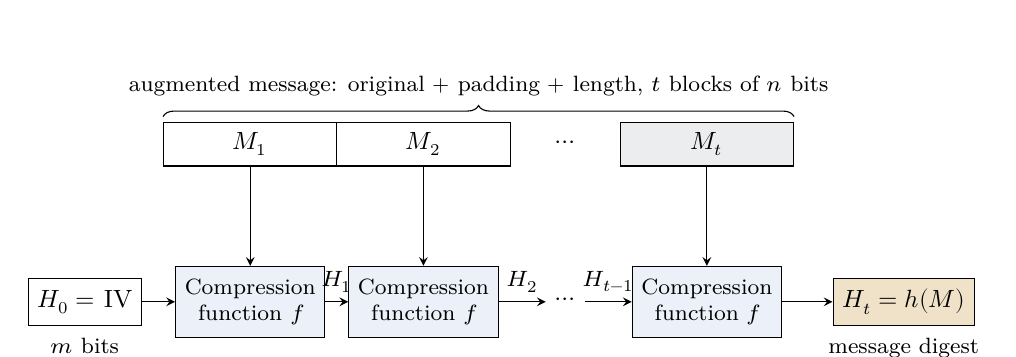
\begin{tikzpicture}[font=\small, >=stealth,
  fbox/.style={draw, fill=acc!8, minimum width=1.7cm, minimum height=0.9cm, align=center, font=\footnotesize},
  mbox/.style={draw, minimum width=2.2cm, minimum height=0.55cm}]
\node[mbox] (m1) at (0,2) {$M_1$};
\node[mbox] (m2) at (2.2,2) {$M_2$};
\node (dots) at (4.0,2) {$\cdots$};
\node[mbox, fill=gray!15] (mt) at (5.8,2) {$M_t$};
\draw[decorate,decoration={brace,amplitude=4pt}] ([yshift=2pt]m1.north west) -- node[above=4pt]{\footnotesize augmented message: original $+$ padding $+$ length, $t$ blocks of $n$ bits} ([yshift=2pt]mt.north east);
\node[draw, minimum width=1cm, minimum height=0.6cm] (h0) at (-2.1,0) {$H_0 = $ IV};
\node[fbox] (f1) at (0,0) {Compression\\function $f$};
\node[fbox] (f2) at (2.2,0) {Compression\\function $f$};
\node at (4.0,0) (d2) {$\cdots$};
\node[fbox] (ft) at (5.8,0) {Compression\\function $f$};
\node[draw, minimum width=1cm, minimum height=0.6cm, fill=gold!20] (ht) at (8.3,0) {$H_t = h(M)$};
\draw[->] (m1) -- (f1); \draw[->] (m2) -- (f2); \draw[->] (mt) -- (ft);
\draw[->] (h0) -- (f1); \draw[->] (f1) -- node[above]{\footnotesize $H_1$} (f2);
\draw[->] (f2) -- node[above]{\footnotesize $H_2$} (d2); \draw[->] (d2) -- node[above]{\footnotesize $H_{t-1}$} (ft);
\draw[->] (ft) -- (ht);
\node[below=1pt of h0, font=\footnotesize] {$m$ bits};
\node[below=1pt of ht, font=\footnotesize] {message digest};
\end{tikzpicture}
\end{center}

The scheme works in five steps.
\begin{enumerate}[nosep]
  \item The message length and padding are appended to the message to create an \textbf{augmented message} whose length is a multiple of $n$, the block size of the compression function.
  \item The augmented message is split into $t$ blocks $M_1, M_2, \dots, M_t$ of $n$ bits each.
  \item Before the iteration starts, the chaining value $H_0$ is set to a fixed public value called the \textbf{IV} (initial value).
  \item Iteration $i$ combines the previous digest with the next block: $H_i = f(H_{i-1}, M_i)$ for $i = 1, \dots, t$.
  \item The last chaining value $H_t$ is the hash of the original message, $h(M) = H_t$.
\end{enumerate}

\textbf{Why it is collision resistant if $f$ is.} Suppose two different messages $M \ne M'$ gave the same final digest $H_t = H'_t$. Then the last compression steps $f(H_{t-1}, M_t)$ and $f(H'_{t-1}, M'_t)$ have equal outputs. If their inputs differ, that is a collision of $f$. If their inputs are equal, then $H_{t-1} = H'_{t-1}$ and the same argument applies one step earlier, and so on backwards. Since $M \ne M'$, the inputs must differ at some step, so a collision of $h$ always yields a collision of $f$. The length field is essential to this argument: it puts the message length in the last block, so two messages of different lengths already differ in their final inputs and cannot be lined up to share a suffix. As a result, the designer only has to make one fixed-size function collision resistant.

\subsection{Compression functions: from scratch or from a block cipher \new}
\likely{``Differentiate Rabin, Davies--Meyer and Miyaguchi--Preneel; why is Rabin weak?'' (3 marks).}

There are two ways to obtain the compression function $f$. In the first, $f$ is \textbf{designed from scratch} specifically for hashing; in the second, an existing \textbf{symmetric-key block cipher} is used as $f$, so that the confidence gained in the cipher carries over.

\textbf{Made from scratch: the MD and SHA families.} The \textbf{Message Digest} family by Rivest has several versions (MD2, MD4, MD5). MD5 is a strengthened MD4 that divides the message into 512-bit blocks and creates a 128-bit digest; this digest turned out to be too short to resist collision attacks. The \textbf{Secure Hash Algorithm} family, the NIST standard also called the Secure Hash Standard (SHS), started with SHA (later SHA-1) and added SHA-224, SHA-256, SHA-384 and SHA-512 (together called SHA-2). All of them are Merkle--Damg\aa rd constructions.
\begin{center}\small
\begin{tabular}{@{}lcccccc@{}}
\toprule
Characteristic & MD5 & SHA-1 & SHA-224 & SHA-256 & SHA-384 & SHA-512\\
\midrule
Maximum message size (bits) & any$^{*}$ & $2^{64} - 1$ & $2^{64} - 1$ & $2^{64} - 1$ & $2^{128} - 1$ & $2^{128} - 1$\\
Block size (bits) & 512 & 512 & 512 & 512 & 1024 & 1024\\
Digest size (bits) & 128 & 160 & 224 & 256 & 384 & 512\\
Number of rounds / steps & 64 & 80 & 64 & 64 & 80 & 80\\
Word size (bits) & 32 & 32 & 32 & 32 & 64 & 64\\
\bottomrule
\end{tabular}
\end{center}
The SHA columns are the slide's table (slide 41); the MD5 column is added for comparison ($^{*}$MD5 records the length modulo $2^{64}$, so it accepts any length). The pattern to remember is that the 32-bit-word members use 512-bit blocks and the 64-bit-word members (SHA-384, SHA-512) use 1024-bit blocks; SHA-384 is SHA-512 with a different IV and a truncated digest.

\textbf{Made from a block cipher.} Let $E_K(P)$ be a block cipher with key $K$ and plaintext $P$. One input of $f$ is the message block $M_i$ and the other is the chaining value $H_{i-1}$; the schemes differ in which goes into the key, which into the plaintext, and what is XORed onto the output.

\begin{center}
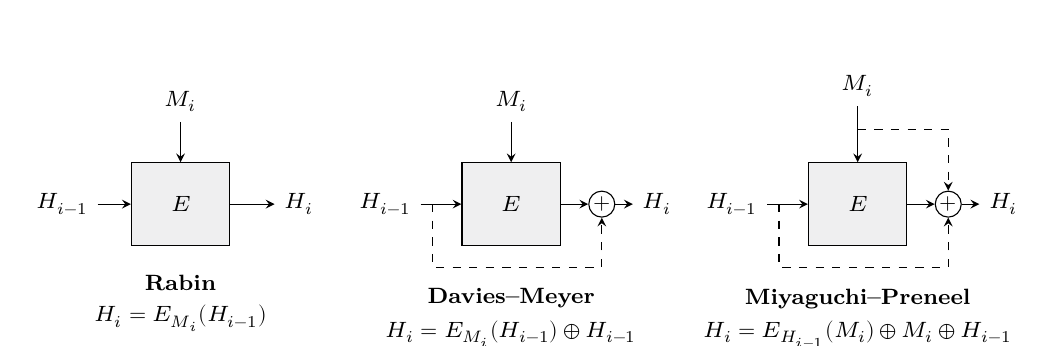
\begin{tikzpicture}[font=\footnotesize, >=stealth,
  enc/.style={draw, fill=gray!12, minimum width=1.25cm, minimum height=1.05cm, align=center},
  xo/.style={draw, circle, inner sep=0pt, minimum size=0.33cm}]
% Rabin
\node[enc] (e1) at (0,0) {$E$};
\node (m1) at (0,1.3) {$M_i$}; \node (h1) at (-1.5,0) {$H_{i-1}$}; \node (o1) at (1.5,0) {$H_i$};
\draw[->] (m1) -- (e1); \draw[->] (h1) -- (e1); \draw[->] (e1) -- (o1);
\node at (0,-1.0) {\textbf{Rabin}};
\node at (0,-1.45) {$H_i = E_{M_i}(H_{i-1})$};
% Davies-Meyer
\begin{scope}[xshift=4.2cm]
\node[enc] (e2) at (0,0) {$E$};
\node (m2) at (0,1.3) {$M_i$}; \node (h2) at (-1.6,0) {$H_{i-1}$};
\node[xo] (x2) at (1.15,0) {$+$}; \node (o2) at (1.85,0) {$H_i$};
\draw[->] (m2) -- (e2); \draw[->] (h2) -- (e2); \draw[->] (e2) -- (x2); \draw[->] (x2) -- (o2);
\draw[->, dashed] (-1.0,0) |- (0.6,-0.8) -| (x2);
\node at (0,-1.2) {\textbf{Davies--Meyer}};
\node at (0,-1.65) {$H_i = E_{M_i}(H_{i-1}) \oplus H_{i-1}$};
\end{scope}
% Miyaguchi-Preneel
\begin{scope}[xshift=8.6cm]
\node[enc] (e3) at (0,0) {$E$};
\node (m3) at (0,1.5) {$M_i$}; \node (h3) at (-1.6,0) {$H_{i-1}$};
\node[xo] (x3) at (1.15,0) {$+$}; \node (o3) at (1.85,0) {$H_i$};
\draw[->] (m3) -- (e3); \draw[->] (h3) -- (e3); \draw[->] (e3) -- (x3); \draw[->] (x3) -- (o3);
\draw[->, dashed] (-1.0,0) |- (0.6,-0.8) -| (x3);
\draw[->, dashed] (0,0.95) -| (x3);
\node at (0,-1.2) {\textbf{Miyaguchi--Preneel}};
\node at (0,-1.65) {$H_i = E_{H_{i-1}}(M_i) \oplus M_i \oplus H_{i-1}$};
\end{scope}
\end{tikzpicture}
\end{center}
In the Rabin and Davies--Meyer pictures the block $M_i$ enters as the \emph{key} (from above) and $H_{i-1}$ as the plaintext; in Miyaguchi--Preneel it is the other way round: $M_i$ is the plaintext and $H_{i-1}$ the key (slide 45). Dashed lines are the feed-forward XORs.

\textbf{Rabin scheme.} Rabin plugs a block cipher directly into Merkle--Damg\aa rd: the message block is used as the key, the previous digest as the plaintext, and the ciphertext is the new digest, $H_i = E_{M_i}(H_{i-1})$. The digest size equals the cipher's block size, so with DES the digest is only 64 bits. Although the scheme is very simple, it is subject to a \textbf{meet-in-the-middle attack}. Because Eve knows every key (the message blocks are her choice), each step can be run \emph{backwards}: $H_{i-1} = D_{M_i}(H_i)$. To forge a message with a given digest $H_t$, she encrypts forward from $H_0$ with about $2^{m/2}$ random choices of the first half of the blocks, stores the intermediate values, then decrypts backward from $H_t$ with about $2^{m/2}$ random choices of the second half, and looks for a common intermediate value. A match gives a full message with digest $H_t$ after only about $2 \times 2^{m/2}$ operations instead of $2^m$; for DES that is about $2^{32}$, which is feasible.

\textbf{Davies--Meyer scheme.} Davies--Meyer is the Rabin scheme plus a \textbf{feed-forward}: the previous digest is XORed onto the cipher output, $H_i = E_{M_i}(H_{i-1}) \oplus H_{i-1}$. Since $H_{i-1}$ now appears both inside the encryption and in the XOR, knowing $H_i$ and $M_i$ no longer lets Eve compute $H_{i-1}$ by decryption, so the backward half of the meet-in-the-middle attack is blocked. This is the protection the slide refers to.

\textbf{Matyas--Meyer--Oseas scheme} (Forouzan, not on the slides). This is the dual of Davies--Meyer: the previous digest is the key (passed through a function $g$ that adapts it to the key size) and the message block is the plaintext, with the block fed forward, $H_i = E_{g(H_{i-1})}(M_i) \oplus M_i$. It is useful when the key and block sizes of the cipher are equal.

\textbf{Miyaguchi--Preneel scheme.} To make the algorithm stronger, the plaintext, the cipher key and the ciphertext are all XORed together to create the new digest: $H_i = E_{H_{i-1}}(M_i) \oplus M_i \oplus H_{i-1}$. It is Matyas--Meyer--Oseas with the chaining value also fed forward. Whirlpool (below) is built on this scheme.

\subsection{SHA-512: overview and parameters \hot}
\asked{End-sem 2025--26 Q5 (7 marks): explain SHA-512 design: message preparation, word expansion, compression function, structure of each round.}
\likely{``Explain SHA-512 with a block diagram: padding, word expansion, round function'' (4--5 marks).}

SHA-512 is the member of the SHA-2 family with the longest digest. It follows the Merkle--Damg\aa rd scheme exactly: the message is padded and given a length field, split into 1024-bit blocks, and each block is fed with the previous 512-bit digest into a compression function; the output of the last block is the 512-bit digest.

\begin{center}
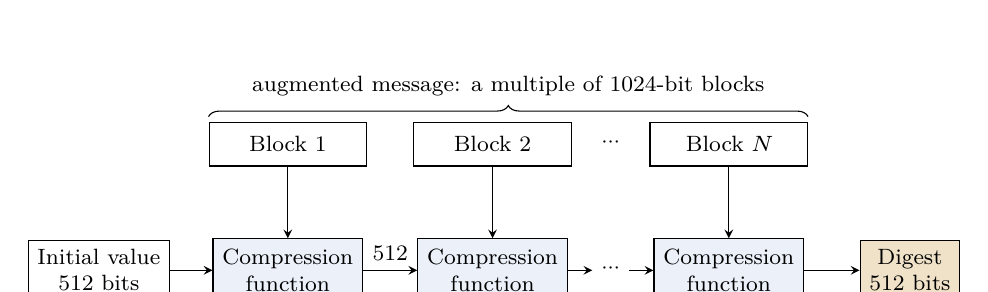
\begin{tikzpicture}[font=\footnotesize, >=stealth,
  blk/.style={draw, minimum width=2.0cm, minimum height=0.55cm},
  cf/.style={draw, fill=acc!8, minimum width=1.9cm, minimum height=0.8cm, align=center}]
\node[blk] (b1) at (0,1.6) {Block 1};
\node[blk] (b2) at (2.6,1.6) {Block 2};
\node (bd) at (4.1,1.6) {$\cdots$};
\node[blk] (bn) at (5.6,1.6) {Block $N$};
\draw[decorate,decoration={brace,amplitude=4pt}] ([yshift=2pt]b1.north west) -- node[above=4pt]{augmented message: a multiple of 1024-bit blocks} ([yshift=2pt]bn.north east);
\node[draw, align=center] (iv) at (-2.4,0) {Initial value\\512 bits};
\node[cf] (c1) at (0,0) {Compression\\function};
\node[cf] (c2) at (2.6,0) {Compression\\function};
\node (cd) at (4.1,0) {$\cdots$};
\node[cf] (cn) at (5.6,0) {Compression\\function};
\node[draw, fill=gold!20, align=center] (dg) at (7.9,0) {Digest\\512 bits};
\draw[->] (b1) -- (c1); \draw[->] (b2) -- (c2); \draw[->] (bn) -- (cn);
\draw[->] (iv) -- (c1); \draw[->] (c1) -- node[above]{512} (c2); \draw[->] (c2) -- (cd); \draw[->] (cd) -- (cn); \draw[->] (cn) -- (dg);
\end{tikzpicture}
\end{center}

SHA-512 is \textbf{word oriented}: a word is 64 bits. Each 1024-bit message block is 16 words, and the 512-bit digest is 8 words, named $A, B, C, D, E, F, G, H$. The parameters are: maximum message length $2^{128} - 1$ bits, block 1024 bits, digest 512 bits, 80 rounds per block, 64-bit words, 80 round constants $K_0, \dots, K_{79}$, and 80 expanded words $W_0, \dots, W_{79}$ per block.

\subsection{SHA-512: padding and length field \new}
\likely{``Compute the number of padding bits for a message of length $L$; is padding needed if the length is already a multiple of 1024?'' (2--3 marks).}

Before processing, Merkle--Damg\aa rd requires the message to be a whole number of blocks, with its length recorded at the end. SHA-512 therefore appends two things to the original message $M$: \textbf{padding}, which is a single 1 bit followed by as many 0 bits as needed, and a \textbf{128-bit length field} holding $|M|$ as an unsigned integer (this is why the maximum message length is $2^{128} - 1$). The total $|M| + |P| + 128$ must be a multiple of 1024, so
\[
|M| + |P| + 128 \equiv 0 \pmod{1024} \quad\Longrightarrow\quad \boxed{\,|P| = (-|M| - 128) \bmod 1024\,}, \qquad 0 \le |P| \le 1023 .
\]
Since the mod gives a value from 0 to 1023, the padding is always less than one block.

\begin{worked}[: padding (Forouzan Example 12.1)]
\textbf{Q.} What is the number of padding bits if the length of the original message is 2590 bits?

\textbf{A.} $|P| = (-2590 - 128) \bmod 1024 = (-2718) \bmod 1024$. Since $-2718 + 3 \times 1024 = 354$, $|P| = \mathbf{354}$ bits: a 1 followed by 353 zeros.\\
\emph{Check}: $2590 + 354 + 128 = 3072 = 3 \times 1024$, so the augmented message is exactly 3 blocks.
\end{worked}

\begin{worked}[: padding, new example]
\textbf{Q.} A message of 5000 bits is hashed with SHA-512. Find the number of padding bits, the number of blocks, and the content of the length field.

\textbf{A.} $|P| = (-5000 - 128) \bmod 1024 = (-5128) \bmod 1024 = -5128 + 6 \times 1024 = \mathbf{1016}$ bits (a 1 followed by 1015 zeros).\\
Total $= 5000 + 1016 + 128 = 6144 = \mathbf{6}$ \textbf{blocks}. The 128-bit length field holds $5000 = $ \ttx{1388} in hex, i.e.\ 115 zero bits followed by \ttx{1001110001000}.\\
\emph{Check}: $6144 / 1024 = 6$ exactly.
\end{worked}

\textbf{Edge cases (Forouzan Examples 12.2--12.3).} A message whose length is \emph{already} a multiple of 1024 still needs padding, because the length field must be added: for $|M| = 1024$, $|P| = (-1152) \bmod 1024 = 896$ and the result is 2 blocks. The formula gives the \textbf{minimum} padding $|P| = 0$ when $|M| \equiv 896 \pmod{1024}$ (the message plus the length field already fill the block) and the \textbf{maximum} $|P| = 1023$ when $|M| \equiv 897 \pmod{1024}$. In the actual standard (FIPS 180) the single 1 bit is always appended, so the padding is at least 1 bit; for $|M| \equiv 896$ this forces a full extra block of 1024 padding bits. A short check of the real rule: the 24-bit message ``abc'' gets $(-24 - 128) \bmod 1024 = 872$ padding bits and fits in one block.

\begin{trap}[: padding arithmetic]
Take the mod of a negative number correctly: add multiples of 1024 until the value lies in $0$--$1023$. Do not forget the 128-bit length field (SHA-1 and SHA-256 use a 64-bit field and 512-bit blocks, giving $|P| = (-|M| - 64) \bmod 512$).
\end{trap}

\subsection{SHA-512: word expansion and the compression function \new}

\textbf{Word expansion.} Each round uses one 64-bit word, but a block has only 16 words, so the block is expanded to 80 words $W_0, \dots, W_{79}$. The first 16 are the block itself; each later word mixes four earlier ones:
\[
W_i = W_{i-16} \oplus \mathrm{RotShift}_{1\text{-}8\text{-}7}(W_{i-15}) \oplus W_{i-7} \oplus \mathrm{RotShift}_{19\text{-}61\text{-}6}(W_{i-2}), \qquad 16 \le i \le 79,
\]
\[
\mathrm{RotShift}_{l\text{-}m\text{-}n}(x) = \mathrm{RotR}_l(x) \oplus \mathrm{RotR}_m(x) \oplus \mathrm{ShL}_n(x),
\]
where $\mathrm{RotR}_i(x)$ rotates $x$ right by $i$ bits (bits leaving on the right re-enter on the left) and $\mathrm{ShL}_i(x)$ shifts $x$ left by $i$ bits, filling with 0s (bits leaving are lost). This is the slides' (Forouzan's) form; see the correction box for the standard's exact operations. Since every later word depends on several earlier ones, a change in one message bit spreads into many of the 80 words.

\textbf{Initial values and constants.} The eight words of $H_0$ are the first 64 bits of the fractional parts of the square roots of the first eight primes (2 to 19); for example $A_0 = $ \ttx{6A09E667F3BCC908} from $\sqrt 2$. The 80 round constants $K_0, \dots, K_{79}$ are the first 64 bits of the fractional parts of the cube roots of the first 80 primes (2 to 409); for example $K_0 = $ \ttx{428A2F98D728AE22} from $\sqrt[3]{2}$. Taking them from irrational numbers shows that the designers hid no trapdoor in the constants (``nothing up my sleeve'' numbers).

\textbf{Compression function.} Processing one block takes 80 rounds. At the start, the eight digest words from the previous block (or the IV) are saved in eight temporary variables. Round $i$ mixes the current $A, \dots, H$ with the word $W_i$ and the constant $K_i$ and produces a new set of eight words. After round 79, the saved values are added to the outputs word by word modulo $2^{64}$; this \textbf{final adding} produces the digest that is passed to the next block (or is the final digest). The final adding is a feed-forward, exactly like Davies--Meyer, and it makes the compression function impossible to run backwards.

\textbf{Structure of each round.} Six of the eight words are simply moved one place right, and only two new words are computed, using two mixers (every $+$ here is addition modulo $2^{64}$):
\[
T_1 = H + \mathrm{Conditional}(E, F, G) + \mathrm{Rotate}(E) + W_i + K_i, \qquad T_2 = \mathrm{Majority}(A, B, C) + \mathrm{Rotate}(A),
\]
\[
H \leftarrow G,\; G \leftarrow F,\; F \leftarrow E,\; E \leftarrow D + T_1,\; D \leftarrow C,\; C \leftarrow B,\; B \leftarrow A,\; A \leftarrow T_1 + T_2 .
\]
The three functions are bitwise (except Rotate, which moves bits within the word):
\begin{itemize}[nosep]
  \item $\mathrm{Majority}(x, y, z) = (x \wedge y) \oplus (y \wedge z) \oplus (z \wedge x)$: each output bit is the majority value of the three input bits.
  \item $\mathrm{Conditional}(x, y, z) = (x \wedge y) \oplus (\overline{x} \wedge z)$: each bit of $x$ acts as a selector, taking the bit of $y$ where $x = 1$ and the bit of $z$ where $x = 0$ (``if $x$ then $y$ else $z$'').
  \item $\mathrm{Rotate}(x) = \mathrm{RotR}_{28}(x) \oplus \mathrm{RotR}_{34}(x) \oplus \mathrm{RotR}_{39}(x)$.
\end{itemize}

\begin{center}
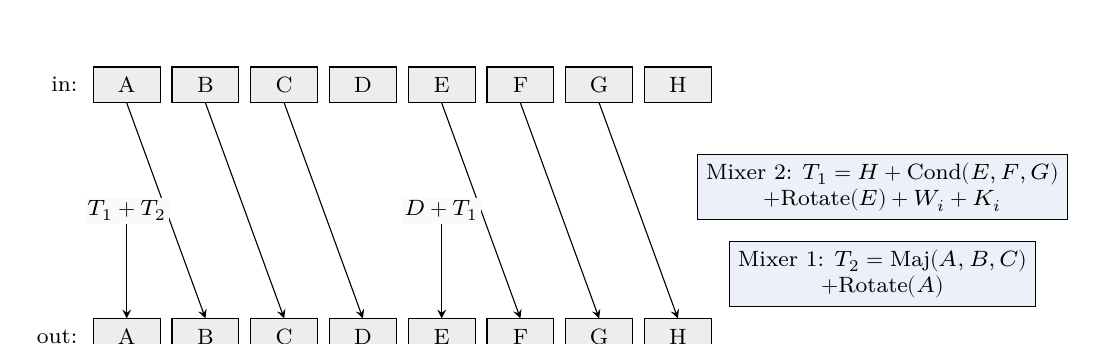
\begin{tikzpicture}[font=\footnotesize, >=stealth,
  reg/.style={draw, fill=gray!15, minimum width=0.85cm, minimum height=0.45cm, inner sep=1pt},
  mix/.style={draw, fill=acc!8, align=center, inner sep=3pt}]
\foreach \n [count=\i] in {A,B,C,D,E,F,G,H} {
  \node[reg] (t\n) at (\i*1.0,3.2) {\n};
  \node[reg] (b\n) at (\i*1.0,0) {\n};
}
\foreach \a/\b in {A/B,B/C,C/D,E/F,F/G,G/H} \draw[->] (t\a.south) -- (b\b.north);
\node[mix] (m2) at (10.6,1.9) {Mixer 2: $T_1 = H + \mathrm{Cond}(E,F,G)$\\$+ \mathrm{Rotate}(E) + W_i + K_i$};
\node[mix] (m1) at (10.6,0.8) {Mixer 1: $T_2 = \mathrm{Maj}(A,B,C)$\\$+ \mathrm{Rotate}(A)$};
\node[font=\footnotesize, fill=white, inner sep=1pt] (xa) at (1.0,1.6) {$T_1 + T_2$};
\node[font=\footnotesize, fill=white, inner sep=1pt] (xe) at (5.0,1.6) {$D + T_1$};
\draw[->] (xa) -- (bA.north); \draw[->] (xe) -- (bE.north);
\node[left=2pt of tA] {in:};
\node[left=2pt of bA] {out:};
\end{tikzpicture}
\end{center}
In Forouzan's notation the new $A$ is called $X$ and the new $E$ is $Y$. Because $A$ and $E$ change every round and the other six words are shifted, every input word affects all eight words within a few rounds.

\begin{mustknow}[: SHA-512 in numbers]
Block 1024 bits $=$ 16 words of 64 bits; digest 512 bits $=$ 8 words $A$--$H$; 80 rounds; 80 words $W_0$--$W_{79}$; 80 constants $K_i$; length field 128 bits; $|P| = (-|M| - 128) \bmod 1024$; max message $2^{128} - 1$ bits; final adding modulo $2^{64}$.
\end{mustknow}

\subsection{Exercises on the SHA-512 operations \new}
\likely{One of the slide exercises (RotR, ShL, Conditional, Majority, Rotate) on given hex words.}

The slide exercises use a \textbf{128-bit} $x$ (real SHA-512 words are 64 bits) and work in hex: a rotation or shift by 12 bits moves the string by 3 hex digits. All results below were recomputed.
\[
x = \texttt{1234 5678 ABCD 2345 3456 5678 ABCD 2468}
\]

\begin{worked}[: RotR, ShL, Conditional, Majority, Rotate (slides 52--56)]
\textbf{RotR$_{12}(x)$.} Rotate right by 12 bits $=$ 3 hex digits: the last three digits \ttx{468} move to the front.\\
\ttx{4681 2345 678A BCD2 3453 4565 678A BCD2}

\textbf{ShL$_{12}(x)$.} Shift left by 3 hex digits: the first three digits \ttx{123} are lost and three 0 digits enter on the right.\\
\ttx{4567 8ABC D234 5345 6567 8ABC D246 8000}

\textbf{Conditional$(x, y, z)$} with $y = $ \ttx{2234 5678 \dots}, $z = $ \ttx{3234 5678 \dots} (the three words differ only in the first digit). For the first digit, $x = 0001$ selects $y$ where $x = 1$ and $z$ where $x = 0$: $(0001 \wedge 0010) \oplus (1110 \wedge 0011) = 0000 \oplus 0010 = 0010 = 2$. For every other digit the three inputs are equal, and Conditional of three equal digits is that digit.\\
Result: \ttx{2234 5678 ABCD 2345 3456 5678 ABCD 2468}

\textbf{Majority$(x, y, z)$}, same $x, y, z$. First digit: $(0001 \wedge 0010) \oplus (0010 \wedge 0011) \oplus (0011 \wedge 0001) = 0000 \oplus 0010 \oplus 0001 = 0011 = 3$. The other digits are unchanged.\\
Result: \ttx{3234 5678 ABCD 2345 3456 5678 ABCD 2468}

\textbf{Rotate$(x) = \mathrm{RotR}_{28}(x) \oplus \mathrm{RotR}_{34}(x) \oplus \mathrm{RotR}_{39}(x)$.} First the three rotations, then the XOR:\\[2pt]
{\small
\begin{tabular}{@{}ll@{}}
$\mathrm{RotR}_{28}(x)$ & \ttx{BCD2 4681 2345 678A BCD2 3453 4565 678A}\\
$\mathrm{RotR}_{34}(x)$ & \ttx{2AF3 491A 048D 159E 2AF3 48D1 4D15 959E}\\
$\mathrm{RotR}_{39}(x)$ & \ttx{F157 9A48 D024 68AC F157 9A46 8A68 ACAC}\\
\midrule
Rotate$(x)$ & \ttx{6776 95D3 F7EC 1AB8 6776 E6C4 8218 5EB8}
\end{tabular}}\\[2pt]
$\mathrm{RotR}_{28}$ is a rotation by 7 hex digits, so it can be done digit-wise; $\mathrm{RotR}_{34}$ and $\mathrm{RotR}_{39}$ are not multiples of 4 and must be done in binary.
\end{worked}

\begin{worked}[: new exercise on 16-bit and 64-bit words]
\textbf{Q.} (a) For the 16-bit words $x = $ \ttx{F0F0}, $y = $ \ttx{AAAA}, $z = $ \ttx{5555}, find Conditional$(x, y, z)$ and Majority$(x, y, z)$. (b) For the 64-bit word $w = $ \ttx{0123 4567 89AB CDEF}, find $\mathrm{RotR}_8(w)$ and $\mathrm{ShL}_8(w)$.

\textbf{A.} (a) Conditional takes $y$ where $x$ is 1 and $z$ where $x$ is 0. $x \wedge y = $ \ttx{A0A0}, $\overline x \wedge z = $ \ttx{0F0F} $\wedge$ \ttx{5555} $= $ \ttx{0505}; Conditional $= $ \ttx{A0A0} $\oplus$ \ttx{0505} $= \mathbf{A5A5}$.\\
Majority: $x \wedge y = $ \ttx{A0A0}, $y \wedge z = $ \ttx{0000} (since $z = \overline y$), $z \wedge x = $ \ttx{5050}; XOR $= \mathbf{F0F0}$. This equals $x$, as it must: $y$ and $z$ disagree in every bit, so $x$ always casts the deciding vote.\\
(b) 8 bits $=$ 2 hex digits. $\mathrm{RotR}_8(w) = $ \ttx{EF01 2345 6789 ABCD} (\ttx{EF} wraps to the front); $\mathrm{ShL}_8(w) = $ \ttx{2345 6789 ABCD EF00} (\ttx{01} is lost, \ttx{00} enters).
\end{worked}

\subsection{Whirlpool}
Whirlpool, designed by Rijmen and Barreto and selected by the NESSIE project (New European Schemes for Signatures, Integrity, and Encryption), is an iterated hash function based on the \textbf{Miyaguchi--Preneel} scheme, in which the compression function is a block cipher: $H_i = E_{H_{i-1}}(M_i) \oplus M_i \oplus H_{i-1}$. The cipher, called W, is a \textbf{modified AES} tailored for this purpose.

\textbf{Parameters.} Block size 512 bits, digest 512 bits, cipher key 512 bits (the previous digest), initial value $H_0$ all 0s, and maximum message length $2^{256} - 1$ bits. The message is padded (a 1 followed by 0s) to an \emph{odd} multiple of 256 bits and then a \textbf{256-bit length field} is appended; an odd multiple of 256 plus 256 is an even multiple, i.e.\ a multiple of 512. For example, $|M| = 1000$ needs $|P| = (-1000 - 256) \bmod 512 = 280$ padding bits, since $1000 + 280 = 1280 = 5 \times 256$ (odd) and $1280 + 256 = 1536 = 3 \times 512$.

\textbf{How the Whirlpool cipher differs from AES.} It uses the same four kinds of transformation, but on a larger state and with all rounds alike:
\begin{itemize}[nosep]
  \item The block and key are 512 bits, held as an $8 \times 8$ matrix of bytes (AES: 128 bits as $4 \times 4$).
  \item There are 10 rounds, each with SubBytes, \textbf{ShiftColumns} (column $j$ is rotated down by $j$ positions, instead of AES's ShiftRows), \textbf{MixRows} (each row is multiplied by a fixed $8 \times 8$ circulant matrix, instead of AES's MixColumns) and AddRoundKey.
  \item Arithmetic is in GF$(2^8)$ with modulus $x^8 + x^4 + x^3 + x^2 + 1$ (AES uses $x^8 + x^4 + x^3 + x + 1$), and the S-box is built from smaller 4-bit boxes.
  \item The round keys are generated by running the same round function on the key, with round constants taken from the S-box in place of a key, instead of AES's separate key-expansion routine.
\end{itemize}

\begin{fixbox}
\begin{itemize}[nosep]
  \item Slide 27: ``$0.69 \times 2^{34}$ seconds or more than 500 years''. In fact $0.69 \times 2^{34}$ s $\approx 376$ years ($2^{34}$ s alone is $\approx 544$ years). The conclusion (secure against preimage attacks) stands.
  \item Slides 54--55 swap the binary for the first digit: Conditional$(0001, 0010, 0011) = 0010 = 2$ and Majority$(0001, 0010, 0011) = 0011 = 3$; the slides print 0011 for Conditional and 0010 for Majority, though the hex results 2 and 3 are right. Both slides also label the third word $x$ instead of $z$.
  \item The exercise $x$ (slides 52--56) is 128 bits, though real SHA-512 words are 64 bits; the rotations on the slides are done on 128 bits, and the results above follow the slides.
  \item Slide 11 prints Problem 4 as $P \approx 1 - e^{-k^2/2N}$; that formula would give $k = 1.18\sqrt N$. The correct one is $P \approx 1 - e^{-k^2/N}$ (as on slide 35), which gives $k = 0.83\sqrt N = 16$.
  \item Slide 40 lists SHA under the ``block cipher'' approach. Forouzan classifies MD and SHA as compression functions \emph{made from scratch} and Rabin, Davies--Meyer, Matyas--Meyer--Oseas and Miyaguchi--Preneel as block-cipher based; write it that way in the exam.
  \item Slides 48 and 51 (from Forouzan) simplify the standard: in FIPS 180 the word expansion uses addition modulo $2^{64}$ and a \emph{right} shift (SHR), not XOR and ShL, and Rotate$(E)$ uses $\mathrm{RotR}_{14} \oplus \mathrm{RotR}_{18} \oplus \mathrm{RotR}_{41}$, not 28-34-39. The slide's ``ShL\dots padding the left by 0s'' is self-contradictory (a left shift fills on the right). For the exam, use the slide formulas.
\end{itemize}
\end{fixbox}

% MNNIT CSN15403 mid-semester papers 2024-25 and 2025-26, fully solved, plus a mock paper in the same style
\clearpage
\section{Previous Year Papers (MNNIT, CSN15403), Fully Solved}\label{sec:pastpapers}

\begin{keybox}[title=What these papers tell you]
\begin{itemize}
  \item \textbf{Format:} 90 minutes, 25 marks, 5--7 questions, ``precise answer with proper justification''. Show every step: tables, matrices, divisions.
  \item \textbf{Sources:} questions come almost word for word from the two standard textbooks: \textbf{Forouzan} (Eve/Alice, $\mathbb{Z}_{100}$, keyed transposition, multiplicative/affine/auto-key, GF$(2^8)$ inverse) and \textbf{Stallings} (``sendmoremoney'' one-time pad, the AES state values).
  \item \textbf{Repeat topics:} Playfair (both years), GF$(2^8)$ inverse (both years), extended Euclid (inverse / Diophantine, both years), DES/AES (both years).
\end{itemize}
\end{keybox}
\begin{center}\small
\begin{tabularx}{\textwidth}{@{}l c c X@{}}
\toprule
Topic & 2024--25 & 2025--26 & In these notes?\\
\midrule
Playfair encryption & 3 & 4 & Section~\ref{sec:playfair}\\
One-time pad / Vigen\`ere & -- & 8 & Sections~\ref{sec:poly}, \ref{sec:otp}\\
Cipher properties, attack types, keyed transposition & 2 + 3 & -- & Sections~\ref{sec:attacks}, \ref{sec:classextra}\\
Modular arithmetic, exponentiation, inverses & 3 & -- & Sections~\ref{sec:modular}--\ref{sec:fermat}\\
Extended Euclid / Diophantine & 5 & 3 & Section~\ref{sec:exteuclid}\\
GF$(2^8)$ polynomial inverse & 4 & 4 & Section~\ref{sec:algebra}\\
DES (Feistel, round function, key schedule) & 5 & -- & Section~\ref{sec:des}\\
AES (ShiftRows, AddRoundKey) & -- & 6 & Section~\ref{sec:aes}\\
\bottomrule
\end{tabularx}
\end{center}
Every topic in these papers is now covered in its own section; the boxes below are one-page summaries for quick revision.

\subsection{Quick-revision method boxes}

\begin{keybox}[title={Extended Euclidean algorithm (Forouzan table): inverse of $b$ mod $n$}]
Columns $q, r_1, r_2, r, t_1, t_2, t$. Start with $r_1 = n$, $r_2 = b$, $t_1 = 0$, $t_2 = 1$. Each row:
\[
q = \lfloor r_1 / r_2 \rfloor,\quad r = r_1 - q\,r_2,\quad t = t_1 - q\,t_2;\qquad\text{then shift: } r_1 \leftarrow r_2,\; r_2 \leftarrow r,\; t_1 \leftarrow t_2,\; t_2 \leftarrow t.
\]
Stop when $r_2 = 0$. If $r_1 = 1$, then $b^{-1} = t_1 \bmod n$. If $r_1 \ne 1$, there is \textbf{no inverse} ($\gcd \ne 1$).
\textbf{Pseudocode:}
\texttt{r1=n; r2=b; t1=0; t2=1; while r2>0 \{ q=r1/r2; r=r1-q*r2; r1=r2; r2=r; t=t1-q*t2; t1=t2; t2=t \}; if r1==1 return t1 mod n}
\end{keybox}

\begin{keybox}[title={Linear Diophantine equation $ax + by = c$}]
Let $d = \gcd(a, b)$. If $d \nmid c$: \textbf{no solution}. Otherwise divide by $d$, find $s, t$ with $as + bt = d$ (extended Euclid), and multiply by $c/d$ to get a particular solution $(x_0, y_0)$.
\textbf{General solution:} $x = x_0 + \frac{b}{d}k$, \; $y = y_0 - \frac{a}{d}k$ \; ($k \in \mathbb{Z}$).
\end{keybox}

\begin{keybox}[title={GF$(p)$ and GF$(2^8)$}]
\textbf{GF$(p)$} = $\{0, \dots, p-1\}$ with $+$ and $\times$ mod a prime $p$. Every non-zero element has an inverse, and ``$a \div b$'' means $a \times b^{-1}$.
\textbf{GF$(2^8)$} elements are polynomials of degree $<8$ with coefficients 0/1 (one byte). \textbf{Add = XOR} (so $+$ and $-$ are the same). Multiply polynomials, then reduce mod $m(x) = x^8 + x^4 + x^3 + x + 1$.
\textbf{Inverse:} the same extended-Euclid table with polynomial division, where every subtraction is an XOR.
\end{keybox}

\begin{keybox}[title=Two classical ciphers and the attack types]
\textbf{Multiplicative:} $C = k_1 P \bmod 26$, with $\gcd(k_1, 26) = 1$. \textbf{Affine:} $C = (k_1 P + k_2) \bmod 26$, decrypted by $P = k_1^{-1}(C - k_2)$.
\textbf{Attacks:} \emph{ciphertext-only} (Eve has only ciphertext), \emph{known-plaintext} (has some plaintext--ciphertext pairs), \emph{chosen-plaintext} (can encrypt plaintext of her choice), \emph{chosen-ciphertext} (can decrypt ciphertext of her choice).
\end{keybox}

% ================================================================
\subsection{Mid-Sem 2024--25, solved}

\textbf{Q1 (2).} \emph{Max characters changed in the ciphertext if one plaintext character changes: (a) multiplicative (b) affine (c) Vigen\`ere (d) auto-key.}\\
(a) \textbf{1}, (b) \textbf{1}, (c) \textbf{1}: each encrypts one character on its own (Vigen\`ere uses a different shift per position, but still one character in, one out).
(d) \textbf{2}. In auto-key the plaintext is also the key: $k_{i+1} = P_i$ (Forouzan; or $k_{i+m} = P_i$ with an $m$-letter keyword, as in our lecture). So changing $P_i$ changes $C_i$ and the one later character it acts as key for.

\textbf{Q2 (3).} \emph{Playfair, key ``GUIDANCE'': ``The key is hidden under the door pad''.}
\begin{center}\small
\begin{minipage}[c]{0.25\textwidth}\centering
\begin{tabular}{|*{5}{c|}}\hline G&U&I/J&D&A\\\hline N&C&E&B&F\\\hline H&K&L&M&O\\\hline P&Q&R&S&T\\\hline V&W&X&Y&Z\\\hline\end{tabular}
\end{minipage}
\begin{minipage}[c]{0.7\textwidth}
Digrams (\ttx{dd} $\to$ \ttx{dx}; \ttx{oo} $\to$ \ttx{ox}; odd length, so the final \ttx{d} becomes \ttx{dx}):\\
\ttx{th ek ey is hi dx de nu nd er th ed ox or pa dx}\\[2pt]
\ttx{PO CL BX DR LG IY IB CG BG LX PO BI LZ LT TG IY}\\[2pt]
(\ttx{er}$\to$\ttx{LX} is a column case; all the others are rectangles.)
\end{minipage}
\end{center}
Ciphertext: \textbf{\ttx{POCLBXDRLGIYIBCGBGLXPOBILZLTTGIY}}.

\textbf{Q3 (3).} \emph{Eve types ``abcdefghij'' on Alice's machine and sees ``CABDEHFGIJ''. Keyed transposition.}\\
(a) \textbf{Chosen-plaintext attack}: Eve chooses the plaintext and sees its encryption.
(b) The pattern repeats every 5: \ttx{abcde}$\to$\ttx{CABDE} and \ttx{fghij}$\to$\ttx{HFGIJ} (positions 3, 1, 2, 4, 5 both times). So the \textbf{key size is 5}.
Encryption key: output takes input positions \textbf{(3 1 2 4 5)}. Decryption key = inverse permutation \textbf{(2 3 1 4 5)}.

\textbf{Q4 (4).} \emph{Inverse of $x^5$ in GF$(2^8)$ mod $m = x^8 + x^4 + x^3 + x + 1$.}
\begin{center}\small\setlength{\tabcolsep}{3pt}
\begin{tabular}{@{}lllllll@{}}
\toprule
$q$ & $r_1$ & $r_2$ & $r$ & $t_1$ & $t_2$ & $t$\\
\midrule
$x^3$ & $x^8{+}x^4{+}x^3{+}x{+}1$ & $x^5$ & $x^4{+}x^3{+}x{+}1$ & 0 & 1 & $x^3$\\
$x{+}1$ & $x^5$ & $x^4{+}x^3{+}x{+}1$ & $x^3{+}x^2{+}1$ & 1 & $x^3$ & $x^4{+}x^3{+}1$\\
$x$ & $x^4{+}x^3{+}x{+}1$ & $x^3{+}x^2{+}1$ & 1 & $x^3$ & $x^4{+}x^3{+}1$ & $x^5{+}x^4{+}x^3{+}x$\\
$x^3{+}x^2{+}1$ & $x^3{+}x^2{+}1$ & 1 & 0 & $x^4{+}x^3{+}1$ & $x^5{+}x^4{+}x^3{+}x$ & $m$\\
 & \textbf{1} & 0 & & $\mathbf{x^5{+}x^4{+}x^3{+}x}$ & & \\
\bottomrule
\end{tabular}
\end{center}
$(x^5)^{-1} = \mathbf{x^5 + x^4 + x^3 + x}$ (byte \ttx{3A}).
Check: using $x^8 = x^4{+}x^3{+}x{+}1$, $x^9 = x^5{+}x^4{+}x^2{+}x$, $x^{10} = x^6{+}x^5{+}x^3{+}x^2$:
$x^5(x^5{+}x^4{+}x^3{+}x) = x^{10}{+}x^9{+}x^8{+}x^6$, and every term cancels in pairs except 1 \checkmark.

\textbf{Q5 (3).}
(i) GF(7): $5 \div 3 = 5 \times 3^{-1} = 5 \times 5 = 25 \equiv \mathbf{4}$ (since $3 \cdot 5 = 15 \equiv 1$).
(ii) $100^{95} \bmod 9$: $100 \equiv 1$, so the answer is $\mathbf{1}$.
$658^{17} \bmod 17$: $658 = 38\cdot17 + 12$, and by Fermat $a^{17} \equiv a \pmod{17}$, so the answer is $\mathbf{12}$.
$145^{102} \bmod 101$: $145 \equiv 44$; Fermat gives $44^{100} \equiv 1$, so $44^{102} \equiv 44^2 = 1936 = 19\cdot101 + 17$, i.e.\ $\mathbf{17}$.
(iii) $7^{-1} \bmod 17 = \mathbf{5}$ ($35 = 2\cdot17 + 1$). $15^{-1} \bmod 99$: $\gcd(15, 99) = 3 \ne 1$, so it \textbf{does not exist}. (That's the trap.)

\textbf{Q6 (5). DES: Feistel structure, round function, key generation.}
\begin{center}
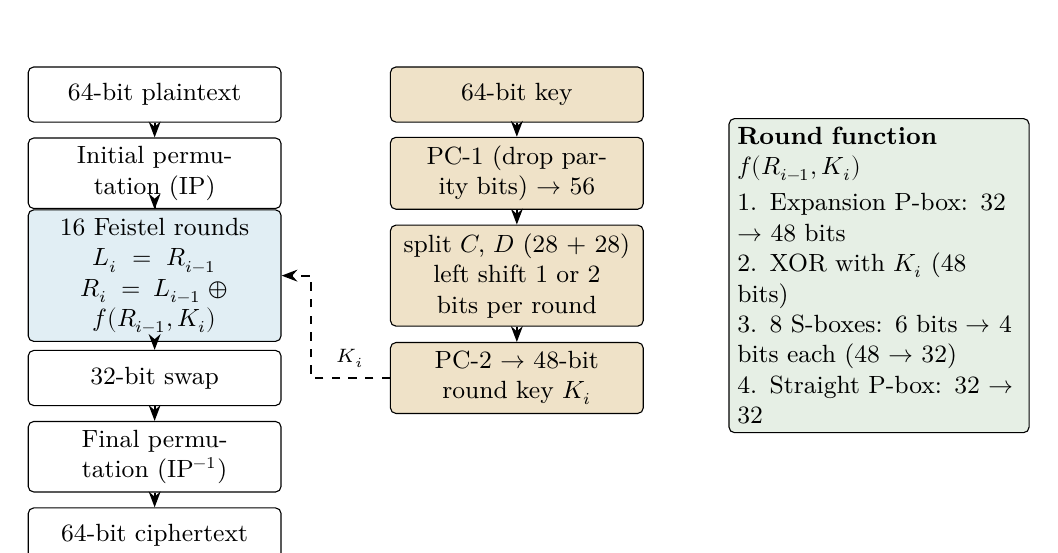
\begin{tikzpicture}[every node/.style={font=\scriptsize}, bx/.style={box,minimum width=30mm,text width=30mm}]
  % data path
  \node[bx] (p) at (0,0) {64-bit plaintext};
  \node[bx] (ip) at (0,-1) {Initial permutation (IP)};
  \node[bx,fill=cyan!10] (r) at (0,-2.3) {16 Feistel rounds\\$L_i = R_{i-1}$\\$R_i = L_{i-1} \oplus f(R_{i-1}, K_i)$};
  \node[bx] (sw) at (0,-3.6) {32-bit swap};
  \node[bx] (fp) at (0,-4.6) {Final permutation (IP$^{-1}$)};
  \node[bx] (c) at (0,-5.6) {64-bit ciphertext};
  \foreach \u/\v in {p/ip,ip/r,r/sw,sw/fp,fp/c} \draw[arr] (\u)--(\v);
  % key schedule
  \node[bx,fill=yellow!20] (k) at (4.6,0) {64-bit key};
  \node[bx,fill=yellow!20] (pc1) at (4.6,-1) {PC-1 (drop parity bits) $\to$ 56};
  \node[bx,fill=yellow!20] (sh) at (4.6,-2.3) {split $C$, $D$ (28 + 28)\\left shift 1 or 2 bits per round};
  \node[bx,fill=yellow!20] (pc2) at (4.6,-3.6) {PC-2 $\to$ 48-bit round key $K_i$};
  \foreach \u/\v in {k/pc1,pc1/sh,sh/pc2} \draw[arr] (\u)--(\v);
  \draw[arr,dashed] (pc2.west) -- node[above]{$K_i$} ++(-1.0,0) |- (r.east);
  % round function
  \node[box,fill=green!12,text width=36mm,align=left] (f) at (9.2,-2.3) {\textbf{Round function} $f(R_{i-1}, K_i)$\\[2pt]
    1. Expansion P-box: 32 $\to$ 48 bits\\2. XOR with $K_i$ (48 bits)\\3. 8 S-boxes: 6 bits $\to$ 4 bits each (48 $\to$ 32)\\4. Straight P-box: 32 $\to$ 32};
\end{tikzpicture}
\end{center}
\begin{itemize}
  \item \textbf{Feistel structure:} each round changes only one half and then swaps the halves. Decryption is the \emph{same} algorithm with the round keys used in reverse ($K_{16}, \dots, K_1$). $f$ need not be invertible.
  \item \textbf{Shifts:} 1 bit in rounds 1, 2, 9, 16; 2 bits in all the others (28 bits in total).
\end{itemize}
\begin{minipage}[t]{0.48\textwidth}\small
\textbf{S-box substitution (pseudocode)}\\
\ttfamily for i = 1 to 8:\\
\hspace*{1em}b = in[6i-5 .. 6i]\quad // 6 bits\\
\hspace*{1em}row = 2*b1 + b6\quad // outer bits\\
\hspace*{1em}col = b2b3b4b5\quad // inner 4 bits\\
\hspace*{1em}out[4i-3 .. 4i] = S[i][row][col]\\
return out\quad // 32 bits
\end{minipage}\hfill
\begin{minipage}[t]{0.48\textwidth}\small
\textbf{Key generation (pseudocode)}\\
\ttfamily K56 = PC1(K64)\\
C = K56[1..28]; D = K56[29..56]\\
for i = 1 to 16:\\
\hspace*{1em}s = (i in \{1,2,9,16\}) ? 1 : 2\\
\hspace*{1em}C = rotl(C, s); D = rotl(D, s)\\
\hspace*{1em}K[i] = PC2(C || D)\quad // 48 bits\\
return K[1..16]
\end{minipage}

\medskip
\textbf{Q7 (5).} \emph{Pseudocode for finding an inverse, and finding $23^{-1}$ in $\mathbb{Z}_{100}$.}
This is the \textbf{extended Euclidean algorithm} (pseudocode in the method box). Mr X's worry is real: an inverse exists only when $\gcd = 1$, and the same algorithm tells him so when it doesn't. Here $\gcd(100, 23) = 1$:
\begin{center}\small
\begin{tabular}{@{}cccccccc@{}}
\toprule
Iter. & $q$ & $r_1$ & $r_2$ & $r$ & $t_1$ & $t_2$ & $t$\\
\midrule
1 & 4 & 100 & 23 & 8 & 0 & 1 & $-4$\\
2 & 2 & 23 & 8 & \textbf{7} & 1 & $-4$ & 9\\
3 & 1 & 8 & 7 & 1 & $-4$ & 9 & $\mathbf{-13}$\\
4 & 7 & 7 & 1 & 0 & 9 & $-13$ & \textbf{100}\\
 & & \textbf{1} & 0 & & $\mathbf{-13}$ & 100 & \\
\bottomrule
\end{tabular}
\end{center}
\begin{enumerate}[leftmargin=1.5em]
  \item \textbf{4 iterations}.
  \item Remainder in iteration 2: $r = \mathbf{7}$.
  \item Coefficient in iteration 4: $t = \mathbf{100}$ (always $\pm n$ in the last step; a useful self-check).
  \item Inverse value in iteration 3: $t = -13$, which is the final answer: $23^{-1} \equiv -13 \equiv \mathbf{87} \pmod{100}$. Check: $23 \times 87 = 2001 = 20\cdot100 + 1$ \checkmark.
\end{enumerate}

% ================================================================
\subsection{Mid-Sem 2025--26, solved}

\textbf{Q1 (8).} \emph{One-time-pad Vigen\`ere; key stream 9 0 1 7 23 15 21 14 11 11 2 8 9.}
\begin{center}\small\setlength{\tabcolsep}{4pt}
\begin{tabular}{@{}l*{13}{c}@{}}
\toprule
Plain & s&e&n&d&m&o&r&e&m&o&n&e&y\\
$P$ & 18&4&13&3&12&14&17&4&12&14&13&4&24\\
Key & 9&0&1&7&23&15&21&14&11&11&2&8&9\\
$P{+}K$ & \hl{27}&4&14&10&\hl{35}&\hl{29}&\hl{38}&18&23&25&15&12&\hl{33}\\
mod 26 & 1&4&14&10&9&3&12&18&23&25&15&12&7\\
Cipher & \textbf{B}&\textbf{E}&\textbf{O}&\textbf{K}&\textbf{J}&\textbf{D}&\textbf{M}&\textbf{S}&\textbf{X}&\textbf{Z}&\textbf{P}&\textbf{M}&\textbf{H}\\
\bottomrule
\end{tabular}
\end{center}
(a) \textbf{\ttx{BEOKJDMSXZPMH}}.
(b) We need $K = (C - P) \bmod 26$ with $P$ = \ttx{cashnotneeded}:
\begin{center}\small\setlength{\tabcolsep}{4pt}
\begin{tabular}{@{}l*{13}{c}@{}}
\toprule
$C$ & B 1&E 4&O 14&K 10&J 9&D 3&M 12&S 18&X 23&Z 25&P 15&M 12&H 7\\
$P$ & c 2&a 0&s 18&h 7&n 13&o 14&t 19&n 13&e 4&e 4&d 3&e 4&d 3\\
$C - P$ & $-1$&4&$-4$&3&$-4$&$-11$&$-7$&5&19&21&12&8&4\\
Key & \textbf{25}&\textbf{4}&\textbf{22}&\textbf{3}&\textbf{22}&\textbf{15}&\textbf{19}&\textbf{5}&\textbf{19}&\textbf{21}&\textbf{12}&\textbf{8}&\textbf{4}\\
\bottomrule
\end{tabular}
\end{center}
Key stream: \textbf{25 4 22 3 22 15 19 5 19 21 12 8 4}. This is the point of the question: for \emph{any} ciphertext there is a key giving \emph{any} plaintext of the same length, which is why a one-time pad can't be broken (Section 13).

\textbf{Q2 (4).} \emph{Inverse of $x^7$ mod $x^8 + x^4 + x^3 + x + 1$.}
\begin{center}\small\setlength{\tabcolsep}{3pt}
\begin{tabular}{@{}lllllll@{}}
\toprule
$q$ & $r_1$ & $r_2$ & $r$ & $t_1$ & $t_2$ & $t$\\
\midrule
$x$ & $x^8{+}x^4{+}x^3{+}x{+}1$ & $x^7$ & $x^4{+}x^3{+}x{+}1$ & 0 & 1 & $x$\\
$x^3{+}x^2{+}x$ & $x^7$ & $x^4{+}x^3{+}x{+}1$ & $x$ & 1 & $x$ & $x^4{+}x^3{+}x^2{+}1$\\
$x^3{+}x^2{+}1$ & $x^4{+}x^3{+}x{+}1$ & $x$ & 1 & $x$ & $x^4{+}x^3{+}x^2{+}1$ & $x^7{+}x{+}1$\\
$x$ & $x$ & 1 & 0 & $x^4{+}x^3{+}x^2{+}1$ & $x^7{+}x{+}1$ & $m$\\
 & \textbf{1} & 0 & & $\mathbf{x^7{+}x{+}1}$ & & \\
\bottomrule
\end{tabular}
\end{center}
$(x^7)^{-1} = \mathbf{x^7 + x + 1}$ (byte \ttx{83}). (Row 2 detail: $x^7 \div (x^4{+}x^3{+}x{+}1)$ gives quotient $x^3{+}x^2{+}x$ and remainder $x$, all with XOR subtraction.)

\textbf{Q3 (4).} \emph{Playfair with the given key matrix: ``Insta Reels Pe Time Waste Na Kar'' (filler X, I/J together).}
\begin{center}\small
\begin{minipage}[c]{0.25\textwidth}\centering
\begin{tabular}{|*{5}{c|}}\hline L&A&R&K&S\\\hline P&U&B&C&D\\\hline E&F&G&H&I/J\\\hline M&N&O&Q&T\\\hline V&W&X&Y&Z\\\hline\end{tabular}
\end{minipage}
\begin{minipage}[c]{0.7\textwidth}
Digrams (\ttx{ee} in ``reels'' $\to$ \ttx{ex}, then re-pair; odd length, so \ttx{r} becomes \ttx{rx}):\\
\ttx{in st ar ex el sp et im ew as te na ka rx}\\[2pt]
\ttx{FT DZ RK GV MP LD IM ET FV RL MI WU SR BR}\\[2pt]
(rows: \ttx{ar}, \ttx{as}, \ttx{ka}; columns: \ttx{st}, \ttx{el}, \ttx{na}, \ttx{rx}; the rest are rectangles)
\end{minipage}
\end{center}
Ciphertext: \textbf{\ttx{FTDZRKGVMPLDIMETFVRLMIWUSRBR}}.
\emph{Trap:} in ``reels'' the \ttx{ee} lands inside one pair (\ttx{r e | e l} would be wrong). Pairing from the start gives \ttx{in st ar \underline{ee}}, so the filler goes in there.

\textbf{Q4 (6).} \emph{AES: (a) ShiftRows, (b) AddRoundKey.}\\
(a) Row $r$ is rotated \textbf{left by $r$ bytes} (row 0 unchanged):
\[
\begin{pmatrix}\mathtt{87}&\mathtt{F2}&\mathtt{4D}&\mathtt{97}\\\mathtt{EC}&\mathtt{6E}&\mathtt{4C}&\mathtt{90}\\\mathtt{4A}&\mathtt{C3}&\mathtt{46}&\mathtt{E7}\\\mathtt{8C}&\mathtt{D8}&\mathtt{95}&\mathtt{A6}\end{pmatrix}
\;\xrightarrow{\text{ShiftRows}}\;
\begin{pmatrix}\mathtt{87}&\mathtt{F2}&\mathtt{4D}&\mathtt{97}\\\mathtt{6E}&\mathtt{4C}&\mathtt{90}&\mathtt{EC}\\\mathtt{46}&\mathtt{E7}&\mathtt{4A}&\mathtt{C3}\\\mathtt{A6}&\mathtt{8C}&\mathtt{D8}&\mathtt{95}\end{pmatrix}
\]
(b) AddRoundKey $=$ \textbf{byte-wise XOR} of state and key. E.g.\ $\mathtt{47} \oplus \mathtt{AC}$: $\;0100\,0111 \oplus 1010\,1100 = 1110\,1011 = EB$.
\[
\begin{pmatrix}\mathtt{47}&\mathtt{40}&\mathtt{A3}&\mathtt{4C}\\\mathtt{37}&\mathtt{D4}&\mathtt{70}&\mathtt{9F}\\\mathtt{94}&\mathtt{E4}&\mathtt{3A}&\mathtt{42}\\\mathtt{ED}&\mathtt{A5}&\mathtt{A6}&\mathtt{BC}\end{pmatrix}
\oplus
\begin{pmatrix}\mathtt{AC}&\mathtt{19}&\mathtt{28}&\mathtt{57}\\\mathtt{77}&\mathtt{FA}&\mathtt{D1}&\mathtt{5C}\\\mathtt{66}&\mathtt{DC}&\mathtt{29}&\mathtt{00}\\\mathtt{F3}&\mathtt{21}&\mathtt{41}&\mathtt{6A}\end{pmatrix}
=
\begin{pmatrix}\boldsymbol{\mathtt{EB}}&\boldsymbol{\mathtt{59}}&\boldsymbol{\mathtt{8B}}&\boldsymbol{\mathtt{1B}}\\\boldsymbol{\mathtt{40}}&\boldsymbol{\mathtt{2E}}&\boldsymbol{\mathtt{A1}}&\boldsymbol{\mathtt{C3}}\\\boldsymbol{\mathtt{F2}}&\boldsymbol{\mathtt{38}}&\boldsymbol{\mathtt{13}}&\boldsymbol{\mathtt{42}}\\\boldsymbol{\mathtt{1E}}&\boldsymbol{\mathtt{84}}&\boldsymbol{\mathtt{E7}}&\boldsymbol{\mathtt{D6}}\end{pmatrix}
\]
Tip: XOR one hex digit at a time ($\mathtt4 \oplus \mathtt A = 0100 \oplus 1010 = 1110 = \mathtt E$, \;$\mathtt7 \oplus \mathtt C = 0111 \oplus 1100 = 1011 = \mathtt B$).

\textbf{Q5 (3).} \emph{Solve $19x + 13y = 20$.}
$\gcd(19, 13) = 1$, and $1 \mid 20$, so solutions exist. Euclid: $19 = 1\cdot13 + 6$, $13 = 2\cdot6 + 1$. Back-substitute:
$1 = 13 - 2\cdot6 = 13 - 2(19 - 13) = 3\cdot13 - 2\cdot19$, so $s = -2$, $t = 3$.
Times 20: $x_0 = -40$, $y_0 = 60$. General solution: $x = -40 + 13k$, $y = 60 - 19k$. Taking $k = 3$: \textbf{$x = -1$, $y = 3$}, so in general \textbf{$x = -1 + 13k$, $y = 3 - 19k$}.
Check: $19(-1) + 13(3) = -19 + 39 = 20$ \checkmark.

% ================================================================
\clearpage
\subsection{Mock Mid-Sem paper (same style), 90 minutes, 25 marks}
\emph{Precise answer with proper justification will be considered to get complete marks. Attempt all questions.}
\begin{center}\small
\begin{tabularx}{\textwidth}{|c|X|c|}
\hline
\textbf{Q} & & \textbf{Marks}\\\hline
1 & What is the maximum number of characters that change in the \emph{ciphertext} if a single plaintext character is changed, for: (a) Hill ($2\times2$) (b) Playfair (c) row--column transposition? (d) In the auto-key cipher (keyword length $m$), if \emph{one ciphertext character} is corrupted in transit, how many plaintext characters come out wrong after decryption? & 2\\\hline
2 & Using the Playfair cipher with the key ``MNNIT ALLAHABAD'' (I/J in one cell, filler X), encrypt ``Jazz night at the hall tomorrow''. & 4\\\hline
3 & Eve types ``abcdefghijkl'' on Alice's computer and the screen shows ``BDACFHEGJLIK''. Alice uses a keyed transposition cipher.
(a) What type of attack is this? (b) What is the key size? (c) Give the encryption and decryption keys. (d) Decrypt ``ETMEETMAONNO''. & 3\\\hline
4 & In GF$(2^8)$ find the inverse of $(x^6 + x^4 + x + 1)$ modulo $(x^8 + x^4 + x^3 + x + 1)$. Verify your answer. & 4\\\hline
5 & (i) In GF(11) find $7 \div 9$. (ii) Find $2^{90} \bmod 13$ and $1000^{999} \bmod 7$. (iii) Find, if they exist, $11^{-1} \bmod 26$, $26^{-1} \bmod 39$ and $17^{-1} \bmod 101$. & 3\\\hline
6 & Solve the linear Diophantine equations, or show there is no solution: (i) $24x + 138y = 18$ (ii) $15x + 21y = 7$. & 3\\\hline
7 & Using the extended Euclidean algorithm, find $47^{-1}$ in $\mathbb{Z}_{120}$. State (a) the number of iterations, (b) the remainder in iteration 2, (c) $t$ in iteration 3. (d) Does $46$ have an inverse in $\mathbb{Z}_{120}$? Justify. & 3\\\hline
8 & AES. State $S = \begin{pmatrix}\mathtt{19}&\mathtt{A0}&\mathtt{9A}&\mathtt{E9}\\\mathtt{3D}&\mathtt{F4}&\mathtt{C6}&\mathtt{F8}\\\mathtt{E3}&\mathtt{E2}&\mathtt{8D}&\mathtt{48}\\\mathtt{BE}&\mathtt{2B}&\mathtt{2A}&\mathtt{08}\end{pmatrix}$, round key $K = \begin{pmatrix}\mathtt{A0}&\mathtt{88}&\mathtt{23}&\mathtt{2A}\\\mathtt{FA}&\mathtt{54}&\mathtt{A3}&\mathtt{6C}\\\mathtt{FE}&\mathtt{2C}&\mathtt{39}&\mathtt{76}\\\mathtt{17}&\mathtt{B1}&\mathtt{39}&\mathtt{05}\end{pmatrix}$.
(a) Apply ShiftRows to $S$. (b) Apply AddRoundKey with $K$ to your result from (a) (skip MixColumns here). & 3\\\hline
\end{tabularx}
\end{center}

\clearpage
\subsection{Mock paper: model answers}

\textbf{M1.} (a) \textbf{2}: one block of 2 letters; both can change. (b) Usually 2 (one digram), but the \textbf{maximum is every remaining character}: changing a letter can create or remove a doubled pair (e.g.\ ``bal\underline{k}'' $\to$ ``bal\underline{l}''), which adds or removes a filler and shifts every later digram. (c) \textbf{1}: transposition only moves letters, so exactly one ciphertext letter (somewhere else) changes. (d) The wrong $P_i$ is then used as the key for $P_{i+m}$, which is used for $P_{i+2m}$, and so on: the error \textbf{propagates to every $m$-th character until the end}.

\textbf{M2.} Key without repeats: M N I T A L H B D, then the rest.
\begin{center}\small
\begin{minipage}[c]{0.25\textwidth}\centering
\begin{tabular}{|*{5}{c|}}\hline M&N&I/J&T&A\\\hline L&H&B&D&C\\\hline E&F&G&K&O\\\hline P&Q&R&S&U\\\hline V&W&X&Y&Z\\\hline\end{tabular}
\end{minipage}
\begin{minipage}[c]{0.7\textwidth}
\ttx{jazznightatthehalltomorrow}, J $\to$ I. Only \ttx{zz} lands in one pair: \ttx{zx}. The \ttx{tt}, \ttx{ll} and \ttx{rr} are each split across pairs (traps!). Odd length, so \ttx{w} becomes \ttx{wx}:\\
\ttx{ia zx zn ig ht at th eh al lt om or ro wx}\\[2pt]
\ttx{TM VY WA BR DN MA ND FL MC DM EA GU UG XY}
\end{minipage}
\end{center}
Ciphertext: \textbf{\ttx{TMVYWABRDNMANDFLMCDMEAGUUGXY}}. (Note \ttx{or}$\to$\ttx{GU} and \ttx{ro}$\to$\ttx{UG}: reversed pairs give reversed output.)

\textbf{M3.} (a) \textbf{Chosen-plaintext}. (b) The pattern repeats every 4 (\ttx{abcd}$\to$\ttx{BDAC}, \ttx{efgh}$\to$\ttx{FHEG}), so the \textbf{key size is 4}.
(c) Encryption key \textbf{(2 4 1 3)}: output position $j$ takes input position key[$j$]. Decryption key = inverse \textbf{(3 1 4 2)}.
(d) Blocks \ttx{ETME | ETMA | ONNO}, each rearranged as positions 3, 1, 4, 2: \textbf{meet me at noon}.

\textbf{M4.} Table ($m = x^8{+}x^4{+}x^3{+}x{+}1$, $b = x^6{+}x^4{+}x{+}1$):
\begin{center}\small\setlength{\tabcolsep}{3pt}
\begin{tabular}{@{}lllllll@{}}
\toprule
$q$ & $r_1$ & $r_2$ & $r$ & $t_1$ & $t_2$ & $t$\\
\midrule
$x^2{+}1$ & $m$ & $x^6{+}x^4{+}x{+}1$ & $x^2$ & 0 & 1 & $x^2{+}1$\\
$x^4{+}x^2$ & $x^6{+}x^4{+}x{+}1$ & $x^2$ & $x{+}1$ & 1 & $x^2{+}1$ & $x^6{+}x^2{+}1$\\
$x{+}1$ & $x^2$ & $x{+}1$ & 1 & $x^2{+}1$ & $x^6{+}x^2{+}1$ & $x^7{+}x^6{+}x^3{+}x$\\
$x{+}1$ & $x{+}1$ & 1 & 0 & $x^6{+}x^2{+}1$ & $x^7{+}x^6{+}x^3{+}x$ & $m$\\
 & \textbf{1} & 0 & & $\mathbf{x^7{+}x^6{+}x^3{+}x}$ & & \\
\bottomrule
\end{tabular}
\end{center}
Inverse $= \mathbf{x^7 + x^6 + x^3 + x}$ (byte \ttx{CA}; i.e.\ $\{53\}^{-1} = \{CA\}$, the standard AES example).\\
Verified: $(x^6{+}x^4{+}x{+}1)(x^7{+}x^6{+}x^3{+}x) \bmod m = 1$.

\textbf{M5.} (i) $9^{-1} \bmod 11 = 5$ ($45 = 4\cdot11 + 1$), so $7 \div 9 = 7 \cdot 5 = 35 \equiv \mathbf{2}$.
(ii) Fermat: $2^{12} \equiv 1 \pmod{13}$ and $90 = 7\cdot12 + 6$, so $2^{90} \equiv 2^6 = 64 \equiv \mathbf{12}$. \;$1000 = 142\cdot7 + 6 \equiv -1$, so $(-1)^{999} = -1 \equiv \mathbf{6}$.
(iii) $11^{-1} \bmod 26 = \mathbf{19}$ ($209 = 8\cdot26 + 1$). $26^{-1} \bmod 39$: $\gcd(26, 39) = 13$, so it \textbf{does not exist}. $17^{-1} \bmod 101 = \mathbf{6}$ ($102 = 101 + 1$).

\textbf{M6.} (i) $\gcd(24, 138) = 6$ and $6 \mid 18$, so solutions exist. Divide by 6: $4x + 23y = 3$. Since $4\cdot6 + 23\cdot(-1) = 1$, times 3 gives $x_0 = 18$, $y_0 = -3$.
General: $x = 18 + 23k$, $y = -3 - 4k$; with $k = -1$: \textbf{$x = -5 + 23k$, $y = 1 - 4k$}. Check: $24(-5) + 138(1) = 18$ \checkmark.
(ii) $\gcd(15, 21) = 3$, and $3 \nmid 7$: \textbf{no solution}. (The left side is always a multiple of 3.)

\textbf{M7.}
\begin{center}\small
\begin{tabular}{@{}cccccccc@{}}
\toprule
Iter. & $q$ & $r_1$ & $r_2$ & $r$ & $t_1$ & $t_2$ & $t$\\
\midrule
1 & 2 & 120 & 47 & 26 & 0 & 1 & $-2$\\
2 & 1 & 47 & 26 & \textbf{21} & 1 & $-2$ & 3\\
3 & 1 & 26 & 21 & 5 & $-2$ & 3 & $\mathbf{-5}$\\
4 & 4 & 21 & 5 & 1 & 3 & $-5$ & 23\\
5 & 5 & 5 & 1 & 0 & $-5$ & 23 & $-120$\\
 & & \textbf{1} & 0 & & \textbf{23} & & \\
\bottomrule
\end{tabular}
\end{center}
(a) \textbf{5 iterations}; (b) \textbf{21}; (c) $\mathbf{-5}$. \;$47^{-1} = \mathbf{23}$ (check: $47 \times 23 = 1081 = 9\cdot120 + 1$ \checkmark).
(d) \textbf{No}: $\gcd(46, 120) = 2 \ne 1$ (both even), so $46x$ is always even mod 120 and can never be 1.

\textbf{M8.} (a) $\begin{pmatrix}\mathtt{19}&\mathtt{A0}&\mathtt{9A}&\mathtt{E9}\\\mathtt{F4}&\mathtt{C6}&\mathtt{F8}&\mathtt{3D}\\\mathtt{8D}&\mathtt{48}&\mathtt{E3}&\mathtt{E2}\\\mathtt{08}&\mathtt{BE}&\mathtt{2B}&\mathtt{2A}\end{pmatrix}$ \quad
(b) XOR with $K$: $\begin{pmatrix}\boldsymbol{\mathtt{B9}}&\boldsymbol{\mathtt{28}}&\boldsymbol{\mathtt{B9}}&\boldsymbol{\mathtt{C3}}\\\boldsymbol{\mathtt{0E}}&\boldsymbol{\mathtt{92}}&\boldsymbol{\mathtt{5B}}&\boldsymbol{\mathtt{51}}\\\boldsymbol{\mathtt{73}}&\boldsymbol{\mathtt{64}}&\boldsymbol{\mathtt{DA}}&\boldsymbol{\mathtt{94}}\\\boldsymbol{\mathtt{1F}}&\boldsymbol{\mathtt{0F}}&\boldsymbol{\mathtt{12}}&\boldsymbol{\mathtt{2F}}\end{pmatrix}$
\;(e.g.\ $\mathtt{19} \oplus \mathtt{A0} = 0001\,1001 \oplus 1010\,0000 = 1011\,1001 = \mathtt{B9}$).

% Exam-pattern drill bank: questions written in the MNNIT CSN15403 mid-sem style, grouped by question type
\clearpage
\section{Exam-Pattern Drill Bank}\label{sec:drill}
Every question type that appeared in the 2024--25 and 2025--26 papers, several times over, with new numbers.
Do each group until the method is automatic. Marks follow the papers. Answers are in Section~\ref{sec:drillans}.

\newcounter{dq}
\newcommand{\dq}[1]{\refstepcounter{dq}\par\medskip\noindent\textbf{E\thedq.} \emph{[#1]}\ }

\subsection*{Type 1: cipher behaviour and attack types (2--3 marks)}
\dq{2} What is the maximum number of characters that change in the ciphertext if a single plaintext character is changed? (a) one-time pad (b) Hill cipher with a $3\times3$ key (c) keyed transposition (d) auto-key ($k_1 = k$, $k_i = P_{i-1}$).

\dq{2} A single \emph{ciphertext} character is corrupted in transit. How many plaintext characters are wrong after decryption? (a) Vigen\`ere (b) Hill ($2\times2$) (c) auto-key ($k_i = P_{i-1}$) (d) Playfair.

\dq{2} Name the attack: (a) Eve only listens to the channel. (b) Eve finds an old printout with a plaintext and its ciphertext. (c) Eve borrows Alice's encryption device for an hour. (d) Eve tricks Bob into decrypting a ciphertext she made up.

\dq{3} Eve uses Alice's computer, types ``abcdefghijkl'' and sees ``DFACEBJLGIKH''. Alice uses a keyed transposition cipher.
(a) What type of attack is this? (b) What is the key size? (c) Find the encryption and decryption keys. (d) Decrypt ``AKATCTANADWT''.

\dq{2} Encrypt ``enemy attacks tonight'' with the keyed transposition key (3 1 4 5 2), padding with ``z''.

\subsection*{Type 2: Playfair (3--4 marks)}
\dq{4} Use the Playfair cipher to encipher ``We meet at the bridge at midnight Jack''. The key is made by filling the first rows with ``CRYPTOGRAPHY'' and the rest with the remaining alphabet (I/J together, filler X).

\dq{3} Encrypt ``Balloon pops at noon'' with this key matrix:
\begin{center}\small\ttfamily
\begin{tabular}{ccccc}K&E&Y&W&O\\R&D&A&B&C\\F&G&H&I/J&L\\M&N&P&Q&S\\T&U&V&X&Z\end{tabular}
\end{center}

\dq{3} The Playfair key is ``SECURITY''. Decrypt \ttx{DAFSAFCFPMHSLGCSAFRTSBFHUV}.

\subsection*{Type 3: GF$(2^8)$ arithmetic (4 marks)}
For all of these, $m(x) = x^8 + x^4 + x^3 + x + 1$.

\dq{4} Find the multiplicative inverse of $x^2$ in GF$(2^8)$ mod $m(x)$.

\dq{4} Find the multiplicative inverse of $(x^3 + 1)$ in GF$(2^8)$ mod $m(x)$.

\dq{4} Find the multiplicative inverse of $x^4$ in GF$(2^8)$ mod $m(x)$.

\dq{4} Find the multiplicative inverse of $x^6$ in GF$(2^8)$ mod $m(x)$.

\dq{3} In GF$(2^8)$: (a) add $(x^6 + x^4 + x^2 + x + 1)$ and $(x^7 + x + 1)$; (b) multiply them mod $m(x)$.

\subsection*{Type 4: GF$(p)$, modular exponentiation, inverses (3 marks)}
\dq{3} (i) In GF(13) find $4 \div 7$, and in GF(17) find $3 \div 5$.
(ii) Find $999^{999} \bmod 10$, $7^{1000} \bmod 13$ and $1234^{4321} \bmod 5$.
(iii) Find, if they exist, $13^{-1} \bmod 47$, $12^{-1} \bmod 30$ and $5^{-1} \bmod 28$.

\dq{3} Find $777^{333} \bmod 7$, $2^{1000} \bmod 7$, $11^{500} \bmod 12$ and $46^{47} \bmod 47$.

\subsection*{Type 5: extended Euclidean algorithm (5 marks)}
\dq{5} Find $17^{-1}$ in $\mathbb{Z}_{43}$ with the extended Euclidean algorithm. State the number of iterations, the remainder in iteration 3, and $t$ in iteration 2.

\dq{5} Mr X wants $38^{-1}$ in $\mathbb{Z}_{180}$. Run the extended Euclidean algorithm and explain what the final row tells him. Which elements of $\{36, 37, 38, 39\}$ \emph{do} have inverses in $\mathbb{Z}_{180}$?

\dq{5} Find $550^{-1} \bmod 1769$. How many iterations are needed? Comment on the answer.

\subsection*{Type 6: linear Diophantine equations (3 marks)}
\dq{3} Solve, or show there is no solution: (i) $21x + 14y = 35$ \quad (ii) $40x + 15y = 110$ \quad (iii) $12x + 18y = 25$.

\dq{3} A shop sells pens for Rs.\,19 and notebooks for Rs.\,13. A student spends exactly Rs.\,220. How many of each did they buy? Is the answer unique?

\subsection*{Type 7: one-time pad / Vigen\`ere with a key stream (8 marks)}
\dq{8} One-time-pad Vigen\`ere: each plaintext letter is shifted by the next number of the key stream.
(a) Encrypt ``meetmeatnoon'' with the key stream 3 19 5 0 24 11 7 2 14 9 25 8.
(b) Using your ciphertext, find a key stream that makes it decrypt to ``holdposition''.
(c) Why does (b) show that Eve can't break this cipher by brute force?

\dq{3} Encrypt ``polyalphabetic'' with the Vigen\`ere keyword ``LEMON''.

\subsection*{Type 8: AES state operations (6 marks)}
\dq{6} AES state (rows) $S = \begin{pmatrix}\mathtt{32}&\mathtt{88}&\mathtt{31}&\mathtt{E0}\\\mathtt{43}&\mathtt{5A}&\mathtt{31}&\mathtt{37}\\\mathtt{F6}&\mathtt{30}&\mathtt{98}&\mathtt{07}\\\mathtt{A8}&\mathtt{8D}&\mathtt{A2}&\mathtt{34}\end{pmatrix}$, key $K = \begin{pmatrix}\mathtt{2B}&\mathtt{28}&\mathtt{AB}&\mathtt{09}\\\mathtt{7E}&\mathtt{AE}&\mathtt{F7}&\mathtt{CF}\\\mathtt{15}&\mathtt{D2}&\mathtt{15}&\mathtt{4F}\\\mathtt{16}&\mathtt{A6}&\mathtt{88}&\mathtt{3C}\end{pmatrix}$.
(a) Apply ShiftRows to $S$. (b) Apply AddRoundKey to $S$ (the original) with $K$.

\dq{3} After ShiftRows the state is $\begin{pmatrix}\mathtt{D4}&\mathtt{E0}&\mathtt{B8}&\mathtt{1E}\\\mathtt{27}&\mathtt{BF}&\mathtt{B4}&\mathtt{41}\\\mathtt{11}&\mathtt{98}&\mathtt{5D}&\mathtt{52}\\\mathtt{AE}&\mathtt{F1}&\mathtt{E5}&\mathtt{30}\end{pmatrix}$. What was it before ShiftRows?

\dq{3} $\bigstar$ (MixColumns, one byte.) A state column is $(\mathtt{87}, \mathtt{6E}, \mathtt{46}, \mathtt{A6})$. Compute the first byte of its MixColumns output, $\mathtt{02}\cdot\mathtt{87} \oplus \mathtt{03}\cdot\mathtt{6E} \oplus \mathtt{46} \oplus \mathtt{A6}$, in GF$(2^8)$.

\subsection*{Type 9: DES (5 marks)}
\dq{2} DES S-box $S_1$ (below). Find the output for the 6-bit inputs (a) \ttx{100011} (b) \ttx{011011} (c) \ttx{110110}.
\begin{center}\scriptsize\setlength{\tabcolsep}{2.5pt}
\begin{tabular}{c|*{16}{c}}
$S_1$ & 0&1&2&3&4&5&6&7&8&9&10&11&12&13&14&15\\\hline
0 & 14&4&13&1&2&15&11&8&3&10&6&12&5&9&0&7\\
1 & 0&15&7&4&14&2&13&1&10&6&12&11&9&5&3&8\\
2 & 4&1&14&8&13&6&2&11&15&12&9&7&3&10&5&0\\
3 & 15&12&8&2&4&9&1&7&5&11&3&14&10&0&6&13
\end{tabular}
\end{center}

\dq{3} DES key schedule. (a) By how many bits in total have $C$ and $D$ been rotated after rounds 2, 9 and 16? (b) Why is the total after round 16 important? (c) How many bits does PC-1 discard, and why?

\dq{5} Explain with a diagram why a Feistel cipher can decrypt with the \emph{same} round function even if $f$ is not invertible. Given one round's output $(L_1, R_1)$ and $K_1$, write $L_0$ and $R_0$.


\subsection*{Type 10: Fermat, Euler, primitive roots (3--4 marks)}
\dq{3} Using Fermat's little theorem, find (i) $6^{10} \bmod 11$ (ii) $3^{12} \bmod 11$ (iii) $2^{-1} \bmod 13$ (iv) $7^{-1} \bmod 19$.

\dq{4} Using Euler's theorem, find the multiplicative inverses: (i) $3^{-1} \bmod 20$ (ii) $7^{-1} \bmod 15$ (iii) $8^{-1} \bmod 77$ (iv) $60^{-1} \bmod 187$ (v) $71^{-1} \bmod 100$.

\dq{3} Find (i) $7^{222} \bmod 11$ (ii) $4^{532} \bmod 11$ (iii) $11^{2024} \bmod 35$.

\dq{4} (i) Show that 3 is a primitive root of 17. (ii) Find all primitive roots of 11. (iii) How many primitive roots does 23 have? Given that 5 is one, find another without building a table.

\dq{3} Find the order of every element of $\mathbb{Z}_7^*$ and identify its primitive roots. Does $\mathbb{Z}_8^*$ have a primitive root? Justify.

\dq{3} Evaluate, stating whether Fermat's theorem applies: (i) $12^{16} \bmod 17$ (ii) $17^{16} \bmod 17$ (iii) $2^{14} \bmod 15$: what does this tell you about 15? (iv) $2^{340} \bmod 341$ turns out to be 1. Is 341 prime?

% ===============================================================
\clearpage
\subsection{Drill bank: model answers}\label{sec:drillans}
\setcounter{dq}{0}
\newcommand{\da}{\refstepcounter{dq}\par\medskip\noindent\textbf{E\thedq.}\ }

\da (a) \textbf{1} (b) \textbf{3}: the whole block can change (c) \textbf{1}: letters only move, so one letter (at a new position) changes (d) \textbf{2}: $C_i$, and $C_{i+1}$ because $P_i$ is the key for the next letter.

\da (a) \textbf{1} (b) \textbf{2}: the whole block decrypts wrongly (c) \textbf{every character from there on}: wrong $P_i$ becomes the key for $P_{i+1}$, which is then wrong, and so on (d) \textbf{2}: one digram.

\da (a) ciphertext-only (b) known-plaintext (c) chosen-plaintext (d) chosen-ciphertext.

\da (a) \textbf{Chosen-plaintext}. (b) \ttx{abcdef}$\to$\ttx{DFACEB} and \ttx{ghijkl}$\to$\ttx{JLGIKH}: the same pattern, so the \textbf{key size is 6}. (It can't be 3: the first output letter, \ttx{d}, comes from outside \ttx{abc}.)
(c) Encryption key \textbf{(4 6 1 3 5 2)}: output $j$ takes input key[$j$]. Decryption key = inverse \textbf{(3 6 4 1 5 2)}.
(d) Blocks \ttx{AKATCT | ANADWT}, taking positions 3, 6, 4, 1, 5, 2 of each: \textbf{attack at dawn}.

\da 19 letters, padded to 20 with one \ttx{z}, in blocks of 5: \ttx{enemy}, \ttx{attac}, \ttx{kston}, \ttx{ightz}. Each block is output as positions 3, 1, 4, 5, 2:
\ttx{enemy}$\to$\ttx{EEMYN}, \ttx{attac}$\to$\ttx{TAACT}, \ttx{kston}$\to$\ttx{TKONS}, \ttx{ightz}$\to$\ttx{HITZG}. Answer: \textbf{\ttx{EEMYNTAACTTKONSHITZG}} (Forouzan's own example).

\da Matrix: \ttx{C R Y P T / O G A H B / D E F I K / L M N Q S / U V W X Z}.
Text: \ttx{we meet at the bridge at midnight iack} (J$\to$I). The \ttx{ee} and \ttx{tt} split across pairs, so no filler is needed; the length is odd, so pad with \ttx{x}:
\ttx{we me et at th eb ri dg ea tm id ni gh ti ac kx}\\
$\to$ \ttx{VF VM KR BY PB KG PE EO FG RS KE QF AB PK OY IZ} \;(\ttx{me}: column; \ttx{id}, \ttx{gh}: rows).\\
Answer: \textbf{\ttx{VFVMKRBYPBKGPEEOFGRSKEQFABPKOYIZ}}.

\da \ttx{balloonpopsatnoon}: \ttx{ba}, then \ttx{ll} is a double, so \ttx{lx} and re-pair: \ttx{lo on po ps at no on}. Even length now, so no padding.
\ttx{ba lx lo on po ps at no on} $\to$ \textbf{\ttx{CB IZ SC ES SY QM RV SE ES}}.
\emph{Trap:} after \ttx{lx}, the \ttx{oo} falls across \ttx{lo | on}, so no second filler is needed.

\da Matrix: \ttx{S E C U R / I T Y A B / D F G H K / L M N O P / Q V W X Z}. Decrypt (row: left; column: up; rectangle: same rule):
\ttx{hi de th eg ol du nd er th eb ri dg ex} $\to$ remove the final filler: \textbf{``hide the gold under the bridge''}.

\da $q$, $r_1$, $r_2$, $r$, $t_1$, $t_2$, $t$:
\begin{center}\small\setlength{\tabcolsep}{3pt}
\begin{tabular}{@{}lllllll@{}}
\toprule
$x^6{+}x^2{+}x$ & $m$ & $x^2$ & $x{+}1$ & 0 & 1 & $x^6{+}x^2{+}x$\\
$x{+}1$ & $x^2$ & $x{+}1$ & 1 & 1 & $x^6{+}x^2{+}x$ & $x^7{+}x^6{+}x^3{+}x{+}1$\\
$x{+}1$ & $x{+}1$ & 1 & 0 & $x^6{+}x^2{+}x$ & $x^7{+}x^6{+}x^3{+}x{+}1$ & $m$\\
\bottomrule
\end{tabular}
\end{center}
$(x^2)^{-1} = \mathbf{x^7 + x^6 + x^3 + x + 1}$ (\ttx{CB}). Row 1: $m \div x^2$ gives $q = x^6{+}x^2{+}x$, $r = x{+}1$.

\da
\begin{center}\small\setlength{\tabcolsep}{3pt}
\begin{tabular}{@{}lllllll@{}}
\toprule
$x^5{+}x^2{+}x{+}1$ & $m$ & $x^3{+}1$ & $x^2$ & 0 & 1 & $x^5{+}x^2{+}x{+}1$\\
$x$ & $x^3{+}1$ & $x^2$ & 1 & 1 & $x^5{+}x^2{+}x{+}1$ & $x^6{+}x^3{+}x^2{+}x{+}1$\\
$x^2$ & $x^2$ & 1 & 0 & $x^5{+}x^2{+}x{+}1$ & $x^6{+}x^3{+}x^2{+}x{+}1$ & $m$\\
\bottomrule
\end{tabular}
\end{center}
$(x^3{+}1)^{-1} = \mathbf{x^6 + x^3 + x^2 + x + 1}$ (\ttx{4F}).

\da
\begin{center}\small\setlength{\tabcolsep}{3pt}
\begin{tabular}{@{}lllllll@{}}
\toprule
$x^4{+}1$ & $m$ & $x^4$ & $x^3{+}x{+}1$ & 0 & 1 & $x^4{+}1$\\
$x$ & $x^4$ & $x^3{+}x{+}1$ & $x^2{+}x$ & 1 & $x^4{+}1$ & $x^5{+}x{+}1$\\
$x{+}1$ & $x^3{+}x{+}1$ & $x^2{+}x$ & 1 & $x^4{+}1$ & $x^5{+}x{+}1$ & $x^6{+}x^5{+}x^4{+}x^2$\\
$x^2{+}x$ & $x^2{+}x$ & 1 & 0 & $x^5{+}x{+}1$ & $x^6{+}x^5{+}x^4{+}x^2$ & $m$\\
\bottomrule
\end{tabular}
\end{center}
$(x^4)^{-1} = \mathbf{x^6 + x^5 + x^4 + x^2}$ (\ttx{74}).

\da
\begin{center}\small\setlength{\tabcolsep}{3pt}
\begin{tabular}{@{}lllllll@{}}
\toprule
$x^2$ & $m$ & $x^6$ & $x^4{+}x^3{+}x{+}1$ & 0 & 1 & $x^2$\\
$x^2{+}x{+}1$ & $x^6$ & $x^4{+}x^3{+}x{+}1$ & 1 & 1 & $x^2$ & $x^4{+}x^3{+}x^2{+}1$\\
$x^4{+}x^3{+}x{+}1$ & $x^4{+}x^3{+}x{+}1$ & 1 & 0 & $x^2$ & $x^4{+}x^3{+}x^2{+}1$ & $m$\\
\bottomrule
\end{tabular}
\end{center}
$(x^6)^{-1} = \mathbf{x^4 + x^3 + x^2 + 1}$ (\ttx{1D}).
\emph{Pattern:} in the first row, $x^k \cdot q$ is always the top part of $m$; the remainder is the low part $x^4{+}x^3{+}x{+}1$ whenever $k \ge 5$.

\da (a) Addition is XOR, so equal terms cancel: $(x^6{+}x^4{+}x^2{+}x{+}1) + (x^7{+}x{+}1) = \mathbf{x^7 + x^6 + x^4 + x^2}$ (\ttx{57} $\oplus$ \ttx{83} $=$ \ttx{D4}).
(b) The product is $x^{13}{+}x^{11}{+}x^9{+}x^8{+}x^6{+}x^5{+}x^4{+}x^3{+}1$. Reduce with $x^8 = x^4{+}x^3{+}x{+}1$ (and $x^9, \dots, x^{13}$ likewise) to get $\mathbf{x^7 + x^6 + 1}$ (\ttx{C1}). This is Stallings' worked example $\{57\}\cdot\{83\} = \{C1\}$.

\da (i) $7^{-1} \bmod 13 = 2$ ($14 \equiv 1$), so $4 \div 7 = 8$. \;$5^{-1} \bmod 17 = 7$ ($35 \equiv 1$), so $3 \div 5 = 21 \equiv 4$. Answers: \textbf{8, 4}.
(ii) $999 \equiv -1 \pmod{10}$, odd power: $\mathbf{9}$. \;$7^{12} \equiv 1 \pmod{13}$ and $1000 = 83\cdot12 + 4$: $7^4 = 2401 \equiv \mathbf{9}$. \;$1234 \equiv -1 \pmod 5$, odd power: $\mathbf{4}$.
(iii) $13^{-1} \bmod 47 = \mathbf{29}$ ($377 = 8\cdot47 + 1$). $12^{-1} \bmod 30$: $\gcd = 6$, \textbf{does not exist}. $5^{-1} \bmod 28 = \mathbf{17}$ ($85 = 3\cdot28 + 1$).

\da $777 = 111\cdot7 \equiv 0$, so the answer is $\mathbf{0}$. (\emph{Trap:} Fermat needs $\gcd(a, p) = 1$; you can't conclude ``$\equiv 1$''.)
$2^3 \equiv 1 \pmod 7$ and $1000 = 333\cdot3 + 1$, so the answer is $\mathbf{2}$. \;$11 \equiv -1 \pmod{12}$, even power: $\mathbf{1}$. \;$46 \equiv -1 \pmod{47}$, odd power: $\mathbf{46}$ (or by Fermat, $a^p \equiv a$).

\da
\begin{center}\small
\begin{tabular}{@{}cccccccc@{}}
\toprule Iter. & $q$ & $r_1$ & $r_2$ & $r$ & $t_1$ & $t_2$ & $t$\\\midrule
1 & 2 & 43 & 17 & 9 & 0 & 1 & $-2$\\
2 & 1 & 17 & 9 & 8 & 1 & $-2$ & $\mathbf{3}$\\
3 & 1 & 9 & 8 & \textbf{1} & $-2$ & 3 & $-5$\\
4 & 8 & 8 & 1 & 0 & 3 & $-5$ & 43\\
 & & 1 & 0 & & $-5$ & & \\\bottomrule
\end{tabular}
\end{center}
\textbf{4 iterations}; remainder in iteration 3 $= \mathbf{1}$; $t$ in iteration 2 $= \mathbf{3}$. \;$17^{-1} = -5 \equiv \mathbf{38}$ (check: $17 \cdot 38 = 646 = 15\cdot43 + 1$ \checkmark).

\da Table: $q = 4, 1, 2, 1, 4$; remainders $28, 10, 8, 2, 0$. The final row has $r_1 = \mathbf{2}$, not 1, so $\gcd(180, 38) = 2$ and \textbf{38 has no inverse} in $\mathbb{Z}_{180}$. The algorithm itself detects the failure.
$180 = 2^2\cdot3^2\cdot5$, so only numbers co-prime to 2, 3 and 5 have inverses: 36 (no), \textbf{37 (yes)}, 38 (no), 39 (no, divisible by 3).

\da Quotients $3, 4, 1, 1, 1, 1, 1, 4, 3$, so \textbf{9 iterations}. The final $t_1 = \mathbf{550}$: $550^{-1} \equiv 550 \pmod{1769}$. \emph{550 is its own inverse}: $550^2 = 302500 = 171\cdot1769 + 1$. (Stallings' example; a surprising answer worth checking rather than doubting.)

\da (i) $\gcd(21, 14) = 7$ and $7 \mid 35$. Divide by 7: $3x + 2y = 5$. Here $x = 1, y = 1$ works, so \textbf{$x = 1 + 2k$, $y = 1 - 3k$}.
(ii) $\gcd(40, 15) = 5$ and $5 \mid 110$. Divide: $8x + 3y = 22$; $x = 2, y = 2$ works, so \textbf{$x = 2 + 3k$, $y = 2 - 8k$}.
(iii) $\gcd(12, 18) = 6$ and $6 \nmid 25$: \textbf{no solution}.

\da $19x + 13y = 220$, $\gcd = 1$. From Euclid, $19(-2) + 13(3) = 1$, so $x_0 = -440$, $y_0 = 660$, and in general $x = -440 + 13k$, $y = 660 - 19k$.
Both must be $\ge 0$: $k \ge 33.9$ and $k \le 34.7$, so $k = 34$: \textbf{2 pens and 14 notebooks} ($38 + 182 = 220$). The non-negative answer is \textbf{unique}.

\da (a) $P + K$: $12{+}3,\allowbreak\ 4{+}19,\allowbreak\ 4{+}5,\allowbreak\ 19{+}0,\allowbreak\ 12{+}24,\allowbreak\ 4{+}11,\allowbreak\ 0{+}7,\allowbreak\ 19{+}2,\allowbreak\ 13{+}14,\allowbreak\ 14{+}9,\allowbreak\ 14{+}25,\allowbreak\ 13{+}8 = 15,\allowbreak\ 23,\allowbreak\ 9,\allowbreak\ 19,\allowbreak\ 36,\allowbreak\ 15,\allowbreak\ 7,\allowbreak\ 21,\allowbreak\ 27,\allowbreak\ 23,\allowbreak\ 39,\allowbreak\ 21$. Mod 26: \textbf{\ttx{PXJTKPHVBXNV}}.
(b) $K = C - P \pmod{26}$ with $P$ = \ttx{holdposition}: \textbf{8 9 24 16 21 1 15 13 8 15 25 8}.
(c) Every 12-letter message is reachable from this ciphertext with some key, and every key is equally likely, so the ciphertext gives no information (perfect secrecy).

\da Key \ttx{LEMONLEMONLEMO}: \textbf{\ttx{ASXMNWTTOOPXUQ}}.

\da (a) Rotate row $r$ left by $r$: $\begin{pmatrix}\mathtt{32}&\mathtt{88}&\mathtt{31}&\mathtt{E0}\\\mathtt{5A}&\mathtt{31}&\mathtt{37}&\mathtt{43}\\\mathtt{98}&\mathtt{07}&\mathtt{F6}&\mathtt{30}\\\mathtt{34}&\mathtt{A8}&\mathtt{8D}&\mathtt{A2}\end{pmatrix}$.
(b) XOR with $K$: $\begin{pmatrix}\mathtt{19}&\mathtt{A0}&\mathtt{9A}&\mathtt{E9}\\\mathtt{3D}&\mathtt{F4}&\mathtt{C6}&\mathtt{F8}\\\mathtt{E3}&\mathtt{E2}&\mathtt{8D}&\mathtt{48}\\\mathtt{BE}&\mathtt{2B}&\mathtt{2A}&\mathtt{08}\end{pmatrix}$ (e.g.\ $\mathtt{32}\oplus\mathtt{2B} = 0011\,0010 \oplus 0010\,1011 = 0001\,1001 = \mathtt{19}$).
These are the official AES (FIPS-197) test values: the initial AddRoundKey of round 0.

\da InvShiftRows rotates row $r$ \textbf{right} by $r$: $\begin{pmatrix}\mathtt{D4}&\mathtt{E0}&\mathtt{B8}&\mathtt{1E}\\\mathtt{BF}&\mathtt{B4}&\mathtt{41}&\mathtt{27}\\\mathtt{5D}&\mathtt{52}&\mathtt{11}&\mathtt{98}\\\mathtt{30}&\mathtt{AE}&\mathtt{F1}&\mathtt{E5}\end{pmatrix}$.

\da $\mathtt{02}\cdot b$ (``xtime''): shift left 1; if a 1 falls off the top, XOR with $\mathtt{1B}$. \;$\mathtt{03}\cdot b = (\mathtt{02}\cdot b) \oplus b$.
$\mathtt{02}\cdot\mathtt{87}$: $1000\,0111 \to 0000\,1110 \oplus 0001\,1011 = \mathtt{15}$. \;$\mathtt{02}\cdot\mathtt{6E} = \mathtt{DC}$ (no overflow), so $\mathtt{03}\cdot\mathtt{6E} = \mathtt{DC} \oplus \mathtt{6E} = \mathtt{B2}$.
$\mathtt{15} \oplus \mathtt{B2} \oplus \mathtt{46} \oplus \mathtt{A6} = \mathtt{A7} \oplus \mathtt{46} \oplus \mathtt{A6} = \mathtt{E1} \oplus \mathtt{A6} = \mathbf{47}$. That is exactly the \ttx{47} in the 2025--26 paper's ``after MixColumns'' state.

\da Row $=$ (first bit, last bit), column $=$ the middle 4 bits.
(a) \ttx{1}\,\ttx{0001}\,\ttx{1}: row 3, column 1 $\to$ 12 $=$ \textbf{\ttx{1100}}.
(b) \ttx{0}\,\ttx{1101}\,\ttx{1}: row 1, column 13 $\to$ 5 $=$ \textbf{\ttx{0101}}.
(c) \ttx{1}\,\ttx{1011}\,\ttx{0}: row 2, column 11 $\to$ 7 $=$ \textbf{\ttx{0111}}.

\da (a) The shifts are 1, 1, 2, 2, 2, 2, 2, 2, 1, 2, 2, 2, 2, 2, 2, 1. Running totals: after round 2 $= \mathbf{2}$, after round 9 $= \mathbf{15}$, after round 16 $= \mathbf{28}$.
(b) 28 is the length of each half, so after round 16 $C$ and $D$ are back where they started. Decryption can then generate the keys in reverse with right shifts.
(c) PC-1 drops \textbf{8 parity bits} (every 8th bit): $64 \to 56$. They are for error checking, not secrecy, so the real key size is 56 bits.

\da One round: $L_1 = R_0$, \;$R_1 = L_0 \oplus f(R_0, K_1)$. To go back:
\[
R_0 = L_1, \qquad L_0 = R_1 \oplus f(L_1, K_1) \quad\text{(since } R_1 \oplus f(R_0, K_1) = L_0 \oplus f \oplus f = L_0\text{)}.
\]
We only ever \emph{recompute} $f$ (on $L_1 = R_0$, which we know) and XOR it away; we never invert $f$. So $f$ can be any function (DES's S-boxes aren't invertible). Diagram: two halves, $f$ box fed by the right half and $K_i$, XOR into the left half, then a swap (see the 2024--25 Q6 answer above).

\da (i) $p = 11$, $11 \nmid 6$: $6^{10} \equiv \mathbf{1}$ directly.
(ii) $3^{12} = 3^{10}\cdot3^2 \equiv 1 \cdot 9 = \mathbf{9}$.
(iii) $2^{-1} \equiv 2^{13-2} = 2^{11} = 2048 = 157\cdot13 + 7$, so $\mathbf{7}$ (check $2\cdot7 = 14 \equiv 1$).
(iv) $7^{-1} \equiv 7^{17} \bmod 19 = \mathbf{11}$ (check $7\cdot11 = 77 = 4\cdot19 + 1$).

\da Use $a^{-1} \equiv a^{\Phi(n) - 1}$.
(i) $\Phi(20) = 8$: $3^7$; since $3^4 = 81 \equiv 1$, $3^7 \equiv 3^3 = 27 \equiv \mathbf{7}$.
(ii) $\Phi(15) = 8$: $7^7$; powers 7, 4, 13, 1, so $7^4 \equiv 1$ and $7^7 \equiv 7^3 \equiv \mathbf{13}$.
(iii) $\Phi(77) = 60$: $8^{59}$, with $59 = 32 + 16 + 8 + 2 + 1$. Table mod 77: $8^1 = 8$, $8^2 = 64$, $8^4 = 15$, $8^8 = 71$, $8^{16} = 36$, $8^{32} = 64$.
Product: $64\cdot36 \to 71$, $\times71 \to 36$, $\times64 \to 71$, $\times8 \to \mathbf{29}$ (check $8\cdot29 = 232 = 3\cdot77 + 1$).
(iv) $\Phi(187) = 160$: $60^{159} \equiv \mathbf{53}$ (check $60\cdot53 = 3180 = 17\cdot187 + 1$).
(v) $\Phi(100) = 40$: $71^{39} \equiv \mathbf{31}$ (check $71\cdot31 = 2201$).
(These are Forouzan's examples. In the exam, extended Euclid is usually faster; Euler is the method they ask for when they name it.)

\da (i) $222 \bmod 10 = 2$, so $7^2 = 49 \equiv \mathbf{5}$. (ii) $532 \bmod 10 = 2$, so $4^2 = 16 \equiv \mathbf{5}$.
(iii) $\gcd(11, 35) = 1$, $\Phi(35) = 24$, $2024 \bmod 24 = 8$, so $11^8$: $11^2 = 121 \equiv 16$, $11^4 \equiv 256 \equiv 11$, $11^8 \equiv 11^2 \equiv \mathbf{16}$. (In fact $11^3 \equiv 1$, and $2024 = 3\cdot674 + 2$.)

\da (i) Chain mod 17: 3, 9, 10, 13, 5, 15, 11, 16, 14, 8, 7, 4, 12, 2, 6, 1. All 16 distinct, so \textbf{yes}. (Fast test: $16 = 2^4$, so only check $3^8 \equiv 16 \ne 1$.)
(ii) $10 = 2\cdot5$: $a$ is a primitive root iff $a^5 \not\equiv 1$ and $a^2 \not\equiv 1$. That gives \textbf{2, 6, 7, 8} ($\Phi(10) = 4$ of them).
(iii) $\Phi(22) = \mathbf{10}$. Every primitive root is $5^k$ with $\gcd(k, 22) = 1$: e.g.\ $5^3 = 125 = 5\cdot23 + 10$, so \textbf{10}. ($5^2 = 2$ is \emph{not} one, since $\gcd(2, 22) \ne 1$.)

\da Orders in $\mathbb{Z}_7^*$: $\mathrm{ord}(1) = 1$, $\mathrm{ord}(2) = 3$, $\mathrm{ord}(3) = 6$, $\mathrm{ord}(4) = 3$, $\mathrm{ord}(5) = 6$, $\mathrm{ord}(6) = 2$. Primitive roots (order $6 = \Phi(7)$): \textbf{3 and 5}.
$\mathbb{Z}_8^* = \{1, 3, 5, 7\}$: $3^2 = 9 \equiv 1$, $5^2 = 25 \equiv 1$, $7^2 = 49 \equiv 1$. Every order is $\le 2 < \Phi(8) = 4$, so there is \textbf{no primitive root}.

\da (i) 17 is prime and $17 \nmid 12$: $\mathbf{1}$. (ii) $17 \mid 17$, so Fermat does \textbf{not} apply: $17^{16} \equiv \mathbf{0}$.
(iii) $2^4 = 16 \equiv 1 \pmod{15}$, so $2^{14} = 2^{12}\cdot2^2 \equiv 4 \ne 1$. If 15 were prime, Fermat would force 1, so \textbf{15 is composite} (Fermat test).
(iv) \textbf{No}: $341 = 11\cdot31$. Passing the Fermat test doesn't prove primality; 341 is a \emph{pseudoprime} to base 2.

% Practice problems + answer key (every answer verified by script)
\clearpage
\section{Practice Problems}\label{sec:practice}
These go beyond the lecture examples, and many contain a trap. Show your working as you would in an exam. Answers start on a new page (Section~\ref{sec:answers}); don't peek.

\newcounter{qn}
\newcommand{\q}{\refstepcounter{qn}\par\medskip\noindent\textbf{Q\theqn.}\ }

\subsection*{A. Security definitions and shift ciphers}

\q A message is worth \$500 and is useful for only 1 hour. Breaking the cipher needs \$100 of computing time and takes 2 hours.
(a) Is the scheme computationally secure? (b) What if breaking it took 30 minutes instead?

\q (a) Alice encrypts with a shift cipher, key 7, then encrypts the result again with key 21. Which single key gives the same ciphertext? Did encrypting twice make it stronger?
(b) Bob says he used a shift cipher with key 29. Which cipher did he really use?
(c) An attacker brute-forcing a shift cipher got readable text by moving every letter \emph{forward} by 16. What was the encryption key?

\q This was made with a shift cipher; the key is unknown. Decrypt it, then say which principle from the course the message states.
\begin{center}\ttx{DROOXOWIUXYGCDROCICDOW}\end{center}

\subsection*{B. Monoalphabetic}

\q Keyword cipher: write the keyword \textbf{SECURITY} (no repeats) under \ttx{a b c \dots}, then continue with the unused letters in alphabetical order.
(a) Encrypt ``meet me at noon''. (b) Decrypt \ttx{IMRLPRHCXSHSFXNANVAHN}.
(c) Which plaintext letter is not disguised at all by this key? Why is this a typical weakness of keyword ciphers?

\q (a) The lecture says a monoalphabetic cipher has $26!$ keys. How many are actually useful, and why?
(b) Is the Caesar cipher a monoalphabetic cipher?
(c) In a 20-letter ciphertext, \ttx{Q} is the most common letter (4 times). Can you conclude \ttx{Q} $=$ e?

\subsection*{C. Playfair}

\q Keyword \textbf{PLAYFAIR EXAMPLE}. Encrypt ``hide the gold in the tree stump''.

\q Keyword \textbf{MONARCHY}. Split ``committee'' into digrams, then encrypt it.

\q Keyword \textbf{NETWORK}. Decrypt \ttx{GCUYOSODNUZY} and write the final, readable message.

\q (a) Under some Playfair key, \ttx{AB} encrypts to \ttx{XY}. What does \ttx{BA} encrypt to? Does it depend on which of the three rules applied?
(b) Can a Playfair plaintext letter ever encrypt to itself?
(c) An intercepted message contains the pair \ttx{QQ} (as one digram), and elsewhere the letter \ttx{J}. Could it be Playfair ciphertext?

\subsection*{D. Hill}

\q Which of these are valid Hill keys (mod 26)? Give the reason for each.
\[
K_1=\begin{pmatrix}2&3\\1&4\end{pmatrix}\;
K_2=\begin{pmatrix}4&2\\3&1\end{pmatrix}\;
K_3=\begin{pmatrix}13&1\\2&1\end{pmatrix}\;
K_4=\begin{pmatrix}5&4\\3&5\end{pmatrix}\;
K_5=\begin{pmatrix}1&4\\3&1\end{pmatrix}
\]

\q $K=\begin{pmatrix}3&3\\2&5\end{pmatrix}$. (a) Encrypt ``help'' with $C = PK$ (the lecture's convention).
(b) A textbook using $C = KP$ gets a different answer. What is it? (c) Why do they differ?

\q $K=\begin{pmatrix}5&8\\17&3\end{pmatrix}$. (a) Find $K^{-1} \bmod 26$ and check it. (b) Decrypt \ttx{EGXJ}.

\q \textbf{Known-plaintext attack.} A $2\times2$ Hill cipher ($C = PK$) encrypts ``help'' to \ttx{PQEX}. Find the key $K$. Then decrypt \ttx{CKJM}, which was sent with the same key.

\subsection*{E. Polyalphabetic}

\q Vigen\`ere, key \textbf{NESO}. Decrypt \ttx{SVWEHIFQLEFOYCKWFJSWYWZSEI}.

\q (a) What does a Vigen\`ere cipher with key \ttx{AAAA} do? And with key \ttx{DDDD}?
(b) In a long Vigen\`ere ciphertext, the sequence \ttx{KWX} appears at positions 10, 34 and 70. What can you say about the key length?
(c) Suppose you know the key length is 5. How would you break it?

\q Autokey, keyword \textbf{KEY}. (a) Encrypt ``meet at noon''.
(b) Encrypt it with ordinary Vigen\`ere (key \ttx{KEY}) as well. Where do the two ciphertexts first differ, and why?
(c) Why must an autokey receiver decrypt strictly left to right?

\subsection*{F. Vernam and one-time pad}

\q (a) $P = \ttx{10110011}$, $K = \ttx{01101010}$. Find $C$. (b) Compute $C \oplus P$. What do you get, and why? (c) Why doesn't (b) weaken a one-time pad?

\q Two ciphertexts were made with the \textbf{same} one-time pad key:
$C_1 = \ttx{JUVUZEXJGN}$, $C_2 = \ttx{YHZOFXYIWY}$. You know $C_1$ is ``meet at noon''. Recover the key and the second message.

\q The ciphertext \ttx{XMCKL} came from a one-time pad. (a) Find a key that decrypts it to ``hello'' and another that decrypts it to ``later''. (b) What does this show?

\q Which of these give \textbf{perfect secrecy}?
(a) A one-time pad whose random key is used for two messages.
(b) Vigen\`ere with a truly random key as long as the message, used once.
(c) Vernam with a random 1,000-bit tape, looped to encrypt a 10,000-bit message.
(d) A key stream produced from a random 128-bit seed by a fixed formula.
(e) A Caesar shift with a randomly chosen key, used once on a one-letter message.

\subsection*{G. Transposition}

\q Rail fence, depth 3. Decrypt \ttx{WECRLTEERDSOEEFEAOCAIVDEN}.

\q Row--column transposition, 4 columns, key \textbf{3 1 4 2}, padded with \ttx{x}. Decrypt \ttx{EEEETTFTAXMMTHREARPY}.

\q (a) A ciphertext has normal English letter frequencies (lots of E, T, A) but is unreadable. Substitution or transposition?
(b) Show that a rail fence of depth 2 is really a row--column transposition. Which rectangle and key?
(c) Encrypt ``retreat now'' with Caesar ($k=3$) and then rail fence (depth 2). Now do it in the other order. Compare the results and explain.

\subsection*{H. Steganography, key counting, primes}

\q A captured note reads: ``\emph{Don't wait, we'll discuss food now.}'' Analysts believe a message is hidden in it and that a Caesar cipher was also used. Recover the message. Which approach from the lecture did the sender use?

\q LSB steganography, 2 LSBs per channel, bits hidden in the order R, G, B.
(a) Hide the bits \ttx{101101} in the pixel $(200, 13, 87)$. What is the new pixel?
(b) What is the largest amount any channel value can change?
(c) How many bytes can a $1024\times768$ image hide at most?
(d) Why must the stego image not be saved as a JPEG?

\q A company of 100 employees uses symmetric keys so that every pair can talk privately.
(a) How many keys are needed? (b) One more employee joins. How many \emph{new} keys are needed?
(c) How many keys would public-key cryptography need for the 101 employees?

\q Columnar transposition with keyword \textbf{LETTER} (repeated letters numbered left to right), padded with \ttx{x}. Decrypt:
\begin{center}\ttx{TOELXCPNOXAPNIMKOTAXTSDTXATUWX}\end{center}

\q Compute: (a) $-19 \bmod 3$ \quad (b) $3 \bmod 19$ \quad (c) $2^{10} \bmod 11$. For (c), what do you notice? Which upcoming theorem does it preview?

\q (a) Classify each as prime, composite or neither: 1, 2, 51, 91, 97, 221.
(b) To test whether 221 is prime by trial division, what is the largest divisor you need to try? Why?
(c) What is wrong with the sentence ``RSA is secure because factoring large prime numbers is hard''?

\q (a) 100 $= 2^2 \cdot 5^2$ has 9 divisors. Find a rule that gets the number of divisors straight from the prime factorisation, and use it for $5040 = 2^4 \cdot 3^2 \cdot 5 \cdot 7$.
(b) Which numbers have \emph{exactly three} divisors? Give three examples.

\subsection*{I. Modular arithmetic}

\q Valid or invalid? (a) $73 \equiv 13 \pmod{12}$ \quad (b) $-17 \equiv 3 \pmod 5$ \quad (c) $100 \equiv 1 \pmod 9$ \quad (d) $-7 \equiv 7 \pmod 7$ \quad (e) $14 \equiv -14 \pmod 6$ \quad (f) $0 \equiv 26 \pmod{13}$ \quad (g) $38 \bmod 12 = 14$

\q Without a calculator: (a) $(1234 \times 5678) \bmod 9$ \quad (b) $7^{100} \bmod 10$ \quad (c) $2^{50} \bmod 7$ \quad (d) $-123 \bmod 10$

\q Work in $\mathbb{Z}_{10}$. (a) Give the additive inverses of 3, 0 and 5.
(b) Give the multiplicative inverses of 3, 7, 9, 5 and 4, where they exist. (c) Explain why 4 can never have one.

\q Find \emph{all} solutions in $\mathbb{Z}_{12}$: (a) $4x \equiv 8 \pmod{12}$ \quad (b) $3x \equiv 8 \pmod{12}$ \quad (c) $5x \equiv 3 \pmod{12}$

\q (a) What time does a 12-hour clock show 100 hours after 9 o'clock? (b) 50 hours before 3 o'clock?
(c) Use additive inverses to explain why decrypting a shift cipher with key $k$ is the same as \emph{encrypting} with key $26 - k$. What is the ``encryption key'' that decrypts Caesar?

\q Rail fence, depth 4. Decrypt \ttx{TIRTHYSETAEEUDHMKNE}. (Careful: the rows are not all the same length.)

\subsection*{J. Modular exponentiation}

\q (Lecture homework 1) Compute $11^{23} \bmod 187$ by repeated squaring. How is the answer related to the lecture's $88^7 \bmod 187$?

\q (Lecture homework 2) Find the last three digits of $175^{209}$.

\q Compute $2^{33} \bmod 30$ (the example on the definition slide). Do it two ways: repeated squaring, and by spotting a cycle in the powers of 2.

\q (a) Find the last two digits of $7^{222}$. (b) Find its last digit.

\q A student computes $5^{117} \bmod 19$ like this: ``$117 \bmod 19 = 3$, so the answer is $5^3 = 125 \equiv 11$.''
(a) What is wrong? (b) Find the correct answer.

\q (a) $100^{101} \bmod 101$ \quad (b) $100^{100} \bmod 101$ \quad (c) $99^{99} \bmod 100$
(d) How many multiplications does repeated squaring need for $a^{100}$, compared with multiplying $a$ by itself over and over? And for $a^{1024}$?

\subsection*{K. GCD and the Euclidean algorithm}

\q (Lecture homework) Find $\gcd(1005, 105)$ with the table method and $\gcd(529, 123)$ with the recursive method. Are 529 and 123 relatively prime? Is either of them prime?

\q True or false? Give a reason or a counterexample for each.
(a) If $\gcd(a, b) = 1$ then $a$ and $b$ are both prime.
(b) Two even numbers can be relatively prime.
(c) Any two consecutive integers $n$ and $n + 1$ are relatively prime.
(d) $\gcd(a, b) = \gcd(a, a + b)$ for all positive $a, b$.
(e) In the table method you can stop as soon as $R = 0$ and read the answer from column $B$.

\q (a) Find $\gcd(89, 55)$ and count the divisions. (b) Why does it take so many steps for such small numbers?

\q A Hill cipher works mod 26. (a) Which values from 1 to 25 can the determinant of a valid key take? How many are there?
(b) Use the Euclidean algorithm to show that $\gcd(13, 26) \ne 1$ but $\gcd(15, 26) = 1$.

\q (a) $\gcd(0, 17)$ \quad (b) $\gcd(17, 17)$ \quad (c) $\gcd(1, 10^{100})$
(d) Someone starts the table method for $\gcd(105, 1005)$ with $A = 105$, $B = 1005$ (the wrong way round). What happens in the first row? Do they still get the right answer?

\subsection*{L. Relatively prime numbers and Euler's totient}

\q (Lecture homework) (a) Use Euclid to decide whether 790 and 121 are relatively prime. (b) Find $\Phi(369)$ and $\Phi(372)$.

\q Spot the mistakes.
(a) A student writes $\Phi(25) = (5-1)(5-1) = 16$.
(b) Another writes $\Phi(1000) = 1000\,(1 - \tfrac12)^3 (1 - \tfrac15)^3$ ``because $1000 = 2^3 \cdot 5^3$''.
(c) A third says $\Phi(12) = \Phi(2)\cdot\Phi(6) = 1 \cdot 2 = 2$.
Give the correct values, and also find $\Phi(27)$, $\Phi(1024)$ and $\Phi(97)$.

\q These are totient questions in disguise. Say why, then answer.
(a) How many of the fractions $\frac{1}{36}, \frac{2}{36}, \dots, \frac{35}{36}$ are already in lowest terms?
(b) How many integers from 1 to 1000 are divisible by neither 2 nor 5?
(c) A ``multiplicative cipher'' encrypts $C = k\cdot P \bmod 26$. How many values of $k$ give a usable cipher?

\q (a) Find \emph{all} $n$ with $\Phi(n) = 4$. (Hint: if a prime $p$ divides $n$, then $p - 1$ divides $\Phi(n)$.)
(b) Show that $\Phi(n)$ is even for every $n \ge 3$.

\q $\bigstar$ Prove that \textbf{no} integer $n$ has $\Phi(n) = 14$.

\q $\bigstar$ RSA with $n = 187$.
(a) Given $187 = 11 \cdot 17$, find $\Phi(187)$.
(b) Check that $e = 7$ and $d = 23$ satisfy $e\cdot d \equiv 1 \pmod{\Phi(n)}$.
(c) Eve doesn't know 11 and 17, but she steals $\Phi(n) = 160$. Show that she can now factor $n$.
(d) What does (c) tell you about keeping $\Phi(n)$ secret?

\subsection*{M. $\bigstar$ Challenge set (mixed topics)}
Each of these hides a trap or needs ideas from two different sections.

\q The \textbf{multiplicative cipher} encrypts $C = k\cdot P \bmod 26$ (a $=0$, \dots, z $=25$).
(a) Why can't $k = 13$ be used? Find two plaintext letters that collide.
(b) Which two letters are \emph{never} disguised, whatever valid $k$ is chosen?
(c) Adding a shift, $C = (kP + b) \bmod 26$, gives the \emph{affine} cipher. How many keys does it have?

\q Alice and Bob use a perfect one-time pad (fresh random key, used once). Alice's answer is either ``YES'' or ``NO''. Eve intercepts a 3-letter ciphertext.
What does Eve learn? Does this contradict perfect secrecy? How should Alice fix it?

\q (a) A message is Vigen\`ere-encrypted with key \ttx{AB}, then the result is encrypted again with key \ttx{BCD}. Show that this is a single Vigen\`ere cipher and find its key.
(b) If the two keys have lengths 4 and 6, how long is the combined key?
(c) Is double Vigen\`ere much stronger?

\q Known plaintext: Vigen\`ere turns \ttx{thequickbrownfox} into \ttx{VYCFNKTIQKQNLUHZ}. Find the key and its length.

\q Find (a) $3^{(3^3)} \bmod 10$ and (b) $(3^3)^3 \bmod 10$. Why are they different?

\q Without calculating the huge numbers: (a) show that $10^{101} + 1$ is divisible by 11; (b) find $(10^{100} + 1) \bmod 101$.

\q Find $\gcd(2^{30} - 1,\; 2^{20} - 1)$ without multiplying anything out.
(Hint: $2^{30} - 1 = 2^{10}(2^{20} - 1) + (2^{10} - 1)$.)

\q A rail fence of depth 2 is applied to \ttx{abcdefghijklmnop} (16 letters), then again to the result, and so on.
(a) After how many encryptions does the original text come back? (b) What if the message had 20 letters?
(c) What does this say about ``encrypt twice for extra security''?

\q (a) Split ``taxxi'' into Playfair digrams using the lecture's rules. What goes wrong, and how do you fix it?
(b) A Playfair ciphertext contains \ttx{RS} and, later, \ttx{SR}. What can an attacker deduce?

\q Hill key $K = \begin{pmatrix}1&2\\0&25\end{pmatrix}$ ($C = PK$).
(a) Show $K^2 \equiv I \pmod{26}$. (b) Encrypt ``hi'', then encrypt the result again.
(c) Look at the first letter of every block. Why is this key a bad choice despite being valid?

\q Brute-force the shift-cipher ciphertext \ttx{FKHHU}. How many readable answers are there? What does this mean for the lecture's claim that brute force reveals the one meaningful plaintext?


\subsection*{N. $\bigstar$ Fermat, Euler, primitive roots}

\q (a) Show $2^{340} \equiv 1 \pmod{341}$ in two lines. (Hint: look at $2^{10}$.)
(b) Show that base 3 exposes 341 as composite, \emph{without} computing $3^{340} \bmod 341$. (Hint: work mod 31.)

\q Find the last two digits of (a) $3^{2024}$ and (b) $2^{2024}$. Careful: can Euler's theorem be used in (b)?

\q 6 is a primitive root of 41. (a) How many primitive roots does 41 have? (b) Find two more without building any table. (c) Explain why $6^2$ is \emph{not} a primitive root.

\q (a) Is 2 a primitive root of 101? Decide with at most two modular powers. (b) Is 2 a primitive root of 17?

\q Toy Diffie--Hellman with $p = 23$ and $g = 5$. Alice's secret is 6 and Bob's is 15.
(a) Find what each sends and the shared key. (b) Why is $g$ chosen to be a primitive root? (c) What would go wrong with $g = 22$?

\q (a) A student computes $4^{-1} \bmod 9$ as $4^{9-2} \bmod 9$. What is wrong, and what is the right answer?
(b) Applying Euler's formula blindly to $6^{-1} \bmod 9$ gives $6^{\Phi(9) - 1} = 6^5 \bmod 9$. What do you get, and what does it show?

\subsection*{O. $\bigstar$ Attacks and Lecture 5 extras}
\q Classify (attack, goal threatened, passive/active), and say whether encryption alone stops it: (a) Eve can't read the CEO's encrypted mail but notices it goes to a law firm every night at 2 a.m.; (b) a buyer receives goods, then claims she never ordered them; (c) Eve resends a captured \emph{encrypted} ``pay Rs.~500 to Eve'' message; (d) a botnet floods a web server.

\q (a) Why is $(k_1, k_2) = (13, 5)$ an illegal affine key? Show two letters that collide. (b) Known plaintext: an affine cipher maps \ttx{e}$\to$\ttx{R} and \ttx{n}$\to$\ttx{Y}. Find the key and decrypt \ttx{KTF}.

\q A Kasiski test finds repeated trigrams at distances 30, 42, 66 and 18. Which key lengths are possible, and which do you try first? Why does this attack fail completely against the one-time pad?

\q Keyed transposition, blocks of 5, encryption key \ttx{4 2 5 1 3}. (a) Find the decryption key. (b) Encrypt \ttx{attackatdawn} (pad with \ttx{z}). (c) The key happens to be its own inverse. Is that a weakness?

\q Hill $2\times2$ (row vectors, $C = PK$). Eve knows \ttx{help} encrypts to \ttx{DPLE}. Recover $K$.

\q Lecture 6 says composing two permutations gives a single permutation, so double transposition adds no strength. Lecture 5 says double transposition defeats the pattern attack. Reconcile the two.

\subsection*{P. $\bigstar$ Extended Euclid, congruences, Diophantine}
\q Full table: $\gcd(1820, 231)$ and $s, t$ with $1820s + 231t = \gcd$.

\q Find $97^{-1} \bmod 1000$ with the table. Without any table, why does $98^{-1} \bmod 1000$ not exist?

\q Solve $35x \equiv 10 \pmod{50}$ (all solutions in $\mathbb{Z}_{50}$). Then $35x \equiv 11 \pmod{50}$.

\q Using $(84)(-19) + (320)(5) = 4$: solve $84x + 320y = 8$ (particular and general) and explain why $84x + 320y = 10$ has no solution.

\subsection*{Q. $\bigstar$ Primes, primality, CRT, discrete logs}
\q 341 passes the Fermat test with base 2 ($2^{340} \equiv 1 \pmod{341}$). Run Miller--Rabin with base 2. Then run it on $2047 = 23 \times 89$ with base 2 and with base 3. What do the results teach you?

\q (a) Solve $x \equiv 1 \ (3),\ 2\ (4),\ 3\ (5)$. (b) Trap: solve $x \equiv 3 \pmod 6$, $x \equiv 5 \pmod 8$, and then $x \equiv 2 \pmod 6$, $x \equiv 5 \pmod 8$. Can the four-step CRT be used?

\q Factor 8051 by Fermat's method. Why is it so fast here?

\q Given that 2 is a primitive root of 11, list all primitive roots of 11 without testing each number. How many should there be?

\q Solve (a) $2^x \equiv 9 \pmod{11}$; (b) $3^x \equiv 4 \pmod{11}$; (c) $3^x \equiv 2 \pmod{11}$.

\q $\operatorname{ord}_{17}(2) = 8$. Can any element of $\mathbb{Z}_{17}^*$ have order 6? Order 16? Which $a \in \{2, 3, 4\}$ is a primitive root?

\q Compute $5^{117} \bmod 19$ with the least work, then explain what the answer says about $\operatorname{ord}_{19}(5)$.

\subsection*{R. $\bigstar$ Algebraic structures and GF$(2^n)$}
\q $\langle \mathbb{Z}_{10}^*, \times\rangle$ is cyclic. Is $\langle \mathbb{Z}_{12}^*, \times\rangle$? Justify with orders.

\q Group, ring or field (and why): $\langle \mathbb{Z}_{11}, +, \times\rangle$; $\langle \mathbb{Z}_{12}, +, \times\rangle$; GF$(2^4)$; $\langle \mathbb{Z}, +, \times\rangle$; $\langle \mathbb{Z}_{9}^*, \times\rangle$.

\q In GF$(2^4)$ with $x^4 + x + 1$: compute $(x^3 + x + 1)(x^2 + 1)$, and find $(x^3 + x^2)^{-1}$ and $x^{-1}$.

\q $|\mathbb{Z}_{15}^*| = 8$. Can it contain an element of order 3? Order 8? Is it cyclic?

\q AES arithmetic: compute $\ttx{57} \cdot \ttx{83}$ and $\ttx{57} \cdot \ttx{13}$ in GF$(2^8)$.

\q $x^4 + x^2 + 1$ has no root in GF(2) (it equals 1 at both $x = 0$ and $x = 1$). Is it irreducible?

\subsection*{S. $\bigstar$ Modern block ciphers, DES, AES}
\q A 1000-byte file is encrypted with AES. How many padding bits, and how many blocks? With DES?

\q Which of these can appear in a non-Feistel cipher: a $32 \times 48$ expansion P-box, a $6 \times 4$ S-box, a $64 \times 64$ straight P-box, a $4 \times 4$ S-box?

\q DES S-box 1: find the outputs for \ttx{101010}, \ttx{110011}, \ttx{010101}.

\q DES key schedule: how far has each half rotated in total after round 3, after round 9, after round 16? Why must the total be 28?

\q One Feistel round: $L_0 = 1010$, $R_0 = 0110$, $f(R_0, K_1) = 1100$. Find $L_1, R_1$, then decrypt them back.

\q Double DES has a 112-bit key. Explain why its strength is only about $2^{57}$, and what the attack needs in memory.

\q AES-128 key expansion: for how many of the words $w_4..w_{43}$ is SubWord applied? How many round keys does AES-256 use?

\q Compute MixColumns of the columns \ttx{[01 01 01 01]}, \ttx{[C6 C6 C6 C6]} and \ttx{[01 00 00 00]}. What does this show?

\q SubBytes maps \ttx{00} to \ttx{63}, not \ttx{00}, even though $00^{-1}$ is defined as $00$. Why?

\subsection*{T. $\bigstar$ RSA}
\q $p = 13$, $q = 17$, $e = 5$: find $d$, encrypt $P = 65$, decrypt.

\q $p = 7$, $q = 13$, $e = 3$. What goes wrong?

\q Two users publish $n_1 = 143$ and $n_2 = 187$. Break both.

\q You learn $n = 3233$ and $\phi(n) = 3120$. Find $p$, $q$ and, for $e = 17$, $d$.

\q $e = 3$, $n$ is 2048 bits, Alice sends $P = 2$. Eve sees $C = 8$. What's wrong?

\subsection*{U. $\bigstar$ ElGamal and ECC}
\q ElGamal: $p = 23$, $e_1 = 5$, $d = 6$. Encrypt $P = 10$ with $r = 3$, and decrypt.

\q Alice reuses $r = 3$ (same keys as above) and sends a second ciphertext $(10, 10)$. Eve knows the first plaintext was 10. Find the second plaintext.

\q $E_{11}(1, 6)$: list all points, count them, and compute $2 \cdot (2, 7)$.

\q Is $y^2 = x^3$ over $\mathbb{Z}_{p}$ allowed as an ECC curve? What does Hasse say about $\#E$ for $p = 101$?

\q ECC-ElGamal on $E_{13}(1, 1)$: $e_1 = (1, 4)$, $d = 3$. Find $e_2$, encrypt $P = (5, 1)$ with $r = 2$, and decrypt.

\subsection*{V. $\bigstar$ Message integrity}
\q For a 128-bit digest give the work for a preimage and for a collision attack (50\%). Which number is the real security level, and why is MD5 broken while a 128-bit AES key isn't?

\q A 40-bit digest: about how many messages give a 50\% chance of a collision?

\q Match each to an attack and a birthday problem: (a) Eve has the stored hash of a password and wants \emph{any} matching password; (b) Eve has a signed contract and its digest and wants a different contract with the same digest; (c) Eve prepares a fair and an unfair contract, each in many reworded versions, looking for a matching pair.

\q SHA-512: padding for a 3000-bit message, number of blocks, and number of words in the expanded schedule per block.

\q Rabin's scheme with DES produces a 64-bit digest. Why is it insecure, and what does Davies--Meyer change?

\q Compute Majority and Conditional for the nibbles $x = 1010$, $y = 1100$, $z = 0110$.

\q 30 students: probability that two share a birthday (approximation and exact).

% ------------------------------------------------------------------
\clearpage
\section{Answer Key}\label{sec:answers}
\setcounter{qn}{0}
\newcommand{\ans}{\refstepcounter{qn}\par\medskip\noindent\textbf{A\theqn.}\ }

\subsection*{A. Security definitions and shift ciphers}

\ans (a) \textbf{Yes.} The cost criterion fails (\$100 $<$ \$500), but the time criterion holds (2 h $>$ 1 h). Meeting \emph{either} criterion is enough.
(b) \textbf{No.} Now it's cheap \emph{and} fast (30 min $<$ 1 h), so neither criterion holds.
\emph{Trap:} thinking both conditions must hold.

\ans (a) $7 + 21 = 28 \equiv \mathbf{2}$. Two shifts combine into one shift, so it is \textbf{no stronger}: still only 25 keys to try.
(b) $29 \bmod 26 = 3$: the \textbf{Caesar cipher}.
(c) Moving forward 16 is the same as moving back 10 ($16 \equiv -10$). The encryption key is \textbf{10}, not 16 (compare the GERMANY example).

\ans \ttx{O} appears 5 times out of 22, so guess \ttx{O} $=$ e: key $= 14 - 4 = \mathbf{10}$. Shift every letter back 10:
\textbf{``the enemy knows the system''}.
This is \textbf{Kerckhoffs's principle} (Shannon's maxim): assume the attacker knows the algorithm; only the key is secret.

\subsection*{B. Monoalphabetic}

\ans Cipher line:
\begin{center}\small\setlength{\tabcolsep}{2.4pt}
\begin{tabular}{@{}l*{26}{c}@{}}
Plain & a&b&c&d&e&f&g&h&i&j&k&l&m&n&o&p&q&r&s&t&u&v&w&x&y&z\\
Cipher & S&E&C&U&R&I&T&Y&A&B&D&F&G&H&J&K&L&M&N&O&P&Q&V&W&X&\hl{Z}
\end{tabular}
\end{center}
(a) \textbf{\ttx{GRROGRSOHJJH}}.
(b) Look each letter up in the \emph{bottom} row: \textbf{``frequency analysis wins''}.
(c) \textbf{z $\to$ Z}: it maps to itself. The keyword uses no late letters, so the end of the alphabet barely moves (w$\to$V, x$\to$W, y$\to$X, z$\to$Z). A short keyword leaves much of the alphabet in near-normal order.

\ans (a) $26! - 1$. The identity permutation (a$\to$A, b$\to$B, \dots) leaves the message unchanged, just like shift key 0.
(b) \textbf{Yes.} Every shift is one particular permutation of the alphabet; Caesar is one of the $26!$.
(c) \textbf{No.} Frequency analysis needs a long ciphertext. In 20 letters the counts are too small to trust (the lecture's example had 120 letters).

\subsection*{C. Playfair}

\ans ``PLAYFAIR EXAMPLE'' without repeats is P L A Y F I R E X M; then B C D G H K N O Q S T U V W Z.
\begin{center}\small\begin{tabular}{|*{5}{c|}}\hline P&L&A&Y&F\\\hline I&R&E&X&M\\\hline B&C&D&G&H\\\hline K&N&O&Q&S\\\hline T&U&V&W&Z\\\hline\end{tabular}\end{center}
Digrams: \ttx{hi de th eg ol di nt he tr \underline{ex} es tu mp}.
\emph{Trap:} in ``tree'', \ttx{t r e e} gives \ttx{tr} then \ttx{ee}, a double in one pair, so it becomes \ttx{ex} and the second \ttx{e} moves on (\ttx{es}).\\
Answer: \textbf{\ttx{BMODZBXDNABEKUDMUIXMMOUVIF}}\;
(\ttx{ex}$\to$\ttx{XM} and \ttx{tu}$\to$\ttx{UV} are row cases; \ttx{de}$\to$\ttx{OD} is a column case; the rest are rectangles.)

\ans \ttx{c o m m i t t e e} $\to$ \ttx{co}, \ttx{mm}$\to$\ttx{mx}, then \ttx{mi}, \ttx{tt}$\to$\ttx{tx}, then \ttx{te}, then \ttx{e} alone $\to$ \ttx{ex}.
Digrams: \textbf{\ttx{co mx mi tx te ex}}.
\emph{Trap:} \ttx{ee} does \emph{not} get a filler: after re-pairing, the two e's are in different pairs.
All six are rectangles: \textbf{\ttx{HM AU AE SZ LK IU}} $\Rightarrow$ \textbf{\ttx{HMAUAESZLKIU}}.

\ans Matrix, then decrypt (row $\to$ left, column $\to$ up, rectangle as usual):
\begin{center}\small\begin{tabular}{|*{5}{c|}}\hline N&E&T&W&O\\\hline R&K&A&B&C\\\hline D&F&G&H&I\\\hline L&M&P&Q&S\\\hline U&V&X&Y&Z\\\hline\end{tabular}\end{center}
\ttx{GC}$\to$\ttx{ia},\; \ttx{UY}$\to$\ttx{zx},\; \ttx{OS}$\to$\ttx{zi},\; \ttx{OD}$\to$\ttx{ni},\; \ttx{NU}$\to$\ttx{ul},\; \ttx{ZY}$\to$\ttx{yx}\;
$\Rightarrow$ \ttx{iazxziniulyx}.\\
Remove the fillers (\ttx{zx z} was a split \ttx{zz}; the final \ttx{x} is padding): \ttx{iazzinjuly}. Decide i/j from context: \textbf{``jazz in july''}.

\ans (a) \textbf{\ttx{YX}}, always. In every rule, each letter's replacement depends only on its own cell and the other letter's cell, not on the order. (Lecture: \ttx{at}$\to$\ttx{RS}, \ttx{ta}$\to$\ttx{SR}; also \ttx{mo}$\to$\ttx{ON}, \ttx{om}$\to$\ttx{NO}.)
(b) \textbf{Never.} Right neighbour, cell below and other-column corner are all different cells.
(c) \textbf{No, for two reasons.} Plaintext pairs never contain two equal letters, and two different cells always map to two different cells, so a ciphertext pair is never doubled. And J never appears in Playfair ciphertext (the shared cell is written I).

\subsection*{D. Hill}

\ans Valid $\iff \gcd(\det K, 26) = 1$, i.e.\ det (mod 26) is odd and not 13.
\begin{center}\small
\begin{tabular}{@{}lllll@{}}
\toprule
& $\det$ & mod 26 & Valid? & Why\\
\midrule
$K_1$ & $8-3=5$ & 5 & \textbf{yes} & odd, not 13\\
$K_2$ & $4-6=-2$ & 24 & \textbf{no} & even (shares factor 2)\\
$K_3$ & $13-2=11$ & 11 & \textbf{yes} & an entry of 13 is fine; only the det matters\\
$K_4$ & $25-12=13$ & 13 & \textbf{no} & shares factor 13\\
$K_5$ & $1-12=-11$ & 15 & \textbf{yes} & negative is fine: $-11+26=15$\\
\bottomrule
\end{tabular}
\end{center}

\ans (a) \ttx{he} $=(7,4)$: $(7\cdot3+4\cdot2,\;7\cdot3+4\cdot5) = (29, 41) \equiv (3, 15) = $ \ttx{DP}.
\ttx{lp} $=(11,15)$: $(33+30,\;33+75) = (63, 108) \equiv (11, 4) = $ \ttx{LE}. Answer: \textbf{\ttx{DPLE}}.\\
(b) $C = KP$ with column vectors: $(3\cdot7+3\cdot4,\;2\cdot7+5\cdot4) = (33,34) \equiv (7,8) = $ \ttx{HI}; $(3\cdot11+3\cdot15,\;2\cdot11+5\cdot15) = (78, 97) \equiv (0,19) = $ \ttx{AT}. Answer: \textbf{\ttx{HIAT}}.\\
(c) $KP$ with $K$ is the same as $PK$ with the \textbf{transpose} $K^T$. Same key numbers, different matrix, so a different cipher. Always state the convention.

\ans (a) $\det K = 15 - 136 = -121 \equiv -121 + 130 = 9$, and $9^{-1} \equiv 3$ (since $27 = 26 + 1$).
For $2\times2$ there is a shortcut: swap the diagonal, negate the other two.
\[
\operatorname{adj}\begin{pmatrix}a&b\\c&d\end{pmatrix} = \begin{pmatrix}d&-b\\-c&a\end{pmatrix}
\quad\Rightarrow\quad
\operatorname{adj}K = \begin{pmatrix}3&-8\\-17&5\end{pmatrix} \equiv \begin{pmatrix}3&18\\9&5\end{pmatrix}
\]
\[
K^{-1} = 3\begin{pmatrix}3&18\\9&5\end{pmatrix} = \begin{pmatrix}9&54\\27&15\end{pmatrix} \equiv \boxed{\begin{pmatrix}9&2\\1&15\end{pmatrix}}
\qquad\text{Check: } KK^{-1} = \begin{pmatrix}53&130\\156&79\end{pmatrix} \equiv I \;\checkmark
\]
(b) \ttx{EG} $=(4,6)$: $(4\cdot9+6\cdot1,\;4\cdot2+6\cdot15) = (42, 98) \equiv (16, 20) = $ \ttx{qu}.
\ttx{XJ} $=(23,9)$: $(207+9,\;46+135) = (216, 181) \equiv (8, 25) = $ \ttx{iz}. Answer: \textbf{quiz}.

\ans Stack the blocks as rows: $P = \begin{pmatrix}7&4\\11&15\end{pmatrix}$ (\ttx{he}, \ttx{lp}), $C = \begin{pmatrix}15&16\\4&23\end{pmatrix}$ (\ttx{PQ}, \ttx{EX}).
Since $C = PK$, we get $K = P^{-1}C$.\\
$\det P = 105 - 44 = 61 \equiv 9$, and $9^{-1} = 3$. So $P^{-1} = 3\begin{pmatrix}15&-4\\-11&7\end{pmatrix} \equiv \begin{pmatrix}19&14\\19&21\end{pmatrix}$.\\
$K = \begin{pmatrix}19&14\\19&21\end{pmatrix}\begin{pmatrix}15&16\\4&23\end{pmatrix} = \begin{pmatrix}341&626\\369&787\end{pmatrix} \equiv \boxed{\begin{pmatrix}3&2\\5&7\end{pmatrix}}$.\\
To decrypt: $\det K = 11$, $11^{-1} = 19$ ($209 = 8\cdot26+1$), $K^{-1} = 19\begin{pmatrix}7&-2\\-5&3\end{pmatrix} \equiv \begin{pmatrix}3&14\\9&5\end{pmatrix}$.
\ttx{CK} $=(2,10) \to (96, 78) \equiv (18, 0) = $ \ttx{sa}; \ttx{JM} $=(9,12) \to (135, 186) \equiv (5, 4) = $ \ttx{fe}. Answer: \textbf{safe}.\\
\emph{Lesson:} Hill is linear, so a few known plaintext--ciphertext pairs reveal the whole key. This only works when $P$ is invertible (here $\det P = 9$).

\subsection*{E. Polyalphabetic}

\ans $P = (C - K) \bmod 26$ with key \ttx{NESONESO\dots}. The first letters, with the negatives fixed:
\begin{center}\small\setlength{\tabcolsep}{4pt}
\begin{tabular}{@{}l*{8}{c}@{}}
\toprule
$C$ & S 18 & V 21 & W 22 & E 4 & H 7 & I 8 & F 5 & Q 16\\
$K$ & N 13 & E 4 & S 18 & O 14 & N 13 & E 4 & S 18 & O 14\\
$C-K$ & 5 & 17 & 4 & \hl{$-10$} & \hl{$-6$} & 4 & \hl{$-13$} & 2\\
mod 26 & 5 f & 17 r & 4 e & 16 q & 20 u & 4 e & 13 n & 2 c\\
\bottomrule
\end{tabular}
\end{center}
Answer: \textbf{``frequency analysis fails here''}.

\ans (a) \ttx{AAAA}: shift 0 everywhere, so \textbf{nothing is encrypted}. \ttx{DDDD}: shift 3 everywhere, which is just the \textbf{Caesar cipher}. A key whose letters are all equal is a shift cipher.
(b) The distances are $34-10=24$ and $70-34=36$ (and $60$). Repeats happen when the same plaintext meets the same part of the key, so the distances are multiples of the key length. The key length divides $\gcd(24,36) = 12$: it is \textbf{1, 2, 3, 4, 6 or 12}, most likely 6 or 12. (This is the Kasiski idea mentioned in the notes.)
(c) Split the ciphertext into 5 groups: letters 1, 6, 11, \dots; 2, 7, 12, \dots; and so on. Each group was shifted by \textbf{one} key letter, so it is a \textbf{Caesar cipher}. Break each with frequency analysis (its most common letter is probably e).

\ans (a) Key stream \ttx{KEY} + \ttx{meetatn} $=$ \ttx{keymeetatn}. Ciphertext: \textbf{\ttx{WICFEXGOHA}}.
(b) Vigen\`ere: \ttx{WICDERXSMX}. They agree on \ttx{WIC} (both use the keyword \ttx{KEY}) and \textbf{differ from letter 4}: Vigen\`ere repeats \ttx{KEY}, while autokey switches to the plaintext \ttx{m, e, e, \dots}
(c) From letter 4 on, the key \emph{is} the plaintext. The receiver learns each key letter only by decrypting an earlier letter first.

\subsection*{F. Vernam and one-time pad}

\ans (a) $C = \ttx{11011001}$.
(b) $C \oplus P = \ttx{01101010} = K$, because $P \oplus K \oplus P = K$. Knowing a plaintext and its ciphertext reveals the key.
(c) That key is used for \textbf{one message only} and then destroyed. Knowing it tells you nothing about any other message.

\ans $K = C_1 - P_1$: J$-$m $= 9-12 = -3 \to 23 = $ x, U$-$e $= 20-4 = 16 = $ q, \dots\ $\Rightarrow K = $ \textbf{\ttx{xqrbzlkvsa}}.
$P_2 = C_2 - K$: Y$-$x $= 24-23 = 1 = $ b, H$-$q $= 7-16 = -9 \to 17 = $ r, \dots\ $\Rightarrow$ \textbf{``bring money''}.
\emph{Lesson:} reusing a pad key is fatal. One known message reveals the other.

\ans (a) $K = C - P$. For ``hello'': \textbf{\ttx{qirzx}}. For ``later'': \textbf{\ttx{mmjgu}}.
(b) Every 5-letter message is possible with some key, so the ciphertext reveals nothing. This is \textbf{perfect secrecy}, and it is why brute force is useless against an OTP.

\ans (a) \textbf{No}: key reuse (see A18).
(b) \textbf{Yes}: that \emph{is} a one-time pad; Vigen\`ere's formula with a perfect key.
(c) \textbf{No}: the key repeats 10 times.
(d) \textbf{No}: only $2^{128}$ possible key streams, so it is at best computationally secure (a stream cipher).
(e) \textbf{Yes}: a random shift used once on one letter is a one-time pad of length 1. Every plaintext letter is equally likely. \emph{Trap:} ``Caesar is weak'' is only true when the key is reused across many letters.

\subsection*{G. Transposition}

\ans 25 letters; the zig-zag repeats every $2(3-1) = 4$ letters. Row 1 holds positions 1, 5, 9, \dots, 25 (7 letters); row 3 holds 3, 7, \dots, 23 (6 letters); row 2 the rest (12).
Cut: \ttx{WECRLTE | ERDSOEEFEAOC | AIVDEN}, then read along the zig-zag: \textbf{``we are discovered flee at once''}.

\ans 20 letters, 4 columns $\Rightarrow$ 5 rows, 5 letters per column.
\emph{Trap:} key \textbf{3 1 4 2} means column 1 is read \emph{third}, column 2 \emph{first}, column 3 \emph{fourth}, column 4 \emph{second}. So the read order is col 2, col 4, col 1, col 3:
col 2 $=$ \ttx{EEEET}, col 4 $=$ \ttx{TFTAX}, col 1 $=$ \ttx{MMTHR}, col 3 $=$ \ttx{EARPY}.
\begin{center}\small
\begin{tabular}{|cccc|}
\hline m&e&e&t\\ m&e&a&f\\ t&e&r&t\\ h&e&p&a\\ r&t&y&\textit{x}\\ \hline
\end{tabular}
\quad Read rows: \textbf{``meet me after the party''} (+ filler x).
\end{center}
(Notice the ciphertext starts \ttx{EEEE}: transposition keeps letters, so the e's stay visible.)

\ans (a) \textbf{Transposition}: it moves letters but never changes them, so the frequencies stay English.
(b) Write the text row by row into a rectangle with \textbf{2 columns} (letters 1, 2 on row 1; 3, 4 on row 2; \dots), then read column 1, then column 2 (key \textbf{1 2}). Column 1 holds the odd-position letters, which is exactly rail fence row 1. For ``neso academy is the best'' both give \ttx{NSAAEYSHBSEOCDMITEET}.
(c) Both orders give \textbf{\ttx{UWHWRHUDQZ}}. Caesar changes each letter whatever its position; transposition moves positions whatever the letter. So they commute, and the order doesn't matter.

\subsection*{H. Steganography, key counting, primes}

\ans First letters: \textbf{D}on't \textbf{w}ait, \textbf{w}e'll \textbf{d}iscuss \textbf{f}ood \textbf{n}ow $\Rightarrow$ \ttx{DWWDFN}. That isn't a word, so undo Caesar (shift back 3): \textbf{ATTACK}.
The sender \textbf{encrypted first, then hid} the ciphertext. Even someone who spots the hidden letters only gets ciphertext.

\ans (a) Bits \ttx{10 | 11 | 01}:
R $200 = \ttx{110010\textbf{00}} \to \ttx{110010\textbf{10}} = 202$;
G $13 = \ttx{000011\textbf{01}} \to \ttx{000011\textbf{11}} = 15$;
B $87 = \ttx{010101\textbf{11}} \to \ttx{010101\textbf{01}} = 85$.
New pixel: $\mathbf{(202, 15, 85)}$.
(b) \textbf{3}: the last two bits can go from \ttx{00} to \ttx{11} ($0 \to 3$) or back. \emph{Trap:} answering 2 because ``2 bits''.
(c) $1024 \cdot 768 \cdot 6 = 4{,}718{,}592$ bits $= \mathbf{589{,}824}$ \textbf{bytes} (576 KB).
(d) JPEG is \textbf{lossy}: compression changes pixel values slightly, which destroys the LSBs. Use a lossless format like PNG (as OpenStego did).

\ans (a) $\frac{100 \cdot 99}{2} = \mathbf{4950}$.
(b) The newcomer needs a key with each of the 100 existing people: \textbf{100} new keys. (Check: $\frac{101 \cdot 100}{2} - 4950 = 5050 - 4950 = 100$.)
(c) One key pair each: \textbf{101 pairs = 202 keys}. It grows linearly instead of roughly $N^2/2$.

\ans Keyword L E T T E R $\to$ E(col 2) $=1$, E(col 5) $=2$, L $=3$, R $=4$, T(col 3) $=5$, T(col 4) $=6$. Key: \textbf{3 1 5 6 2 4}.
30 letters, 6 columns $\Rightarrow$ 5 letters per column. Cut the ciphertext into fives and put them back in read order (col 2, 5, 1, 6, 3, 4):
col 2 $=$ \ttx{TOELX}, col 5 $=$ \ttx{CPNOX}, col 1 $=$ \ttx{APNIM}, col 6 $=$ \ttx{KOTAX}, col 3 $=$ \ttx{TSDTX}, col 4 $=$ \ttx{ATUWX}.
\begin{center}\small
\begin{tabular}{|cccccc|}\hline a&t&t&a&c&k\\ p&o&s&t&p&o\\ n&e&d&u&n&t\\ i&l&t&w&o&a\\ m&\textit{x}&\textit{x}&\textit{x}&\textit{x}&\textit{x}\\\hline\end{tabular}
\quad Rows: \textbf{``attack postponed until two am''}
\end{center}

\ans (a) $-19 = (-7)\cdot 3 + \mathbf{2}$, so the answer is \textbf{2}. \emph{Trap:} not $-1$; the remainder must be in $0, 1, 2$.
(b) $3 = 0 \cdot 19 + 3$, so the answer is \textbf{3}. A smaller number mod a bigger one is itself.
(c) $2^{10} = 1024 = 93 \cdot 11 + 1$, so the answer is \textbf{1}. Here 11 is prime and the exponent is $11 - 1$, which previews \textbf{Fermat's theorem}: $a^{p-1} \equiv 1 \pmod p$.

\ans (a) 1: \textbf{neither} (only one divisor). 2: \textbf{prime}. $51 = 3 \cdot 17$: composite. $91 = 7 \cdot 13$: composite. 97: \textbf{prime}. $221 = 13 \cdot 17$: composite.
\emph{Traps:} 51, 91 and 221 all end in 1 and ``look'' prime.
(b) Up to $\sqrt{221} \approx 14.9$, so the primes \textbf{2, 3, 5, 7, 11, 13}. If $n = ab$ with both $a, b > \sqrt n$, then $ab > n$, which is impossible, so one factor must be $\le \sqrt n$. Here 13 works: $221 = 13 \cdot 17$.
(c) Primes can't be factored. The hard problem is \textbf{factoring the product} $n = p \cdot q$ of two large primes.

\ans (a) A divisor of $p^a q^b \cdots$ picks each exponent from $0$ to $a$, $0$ to $b$, \dots, so the count is $(a+1)(b+1)\cdots$
Check: $100 = 2^2 5^2 \to 3 \cdot 3 = 9$ \checkmark. \;$5040 \to (4+1)(2+1)(1+1)(1+1) = \mathbf{60}$.
(b) Exactly 3 divisors means $(a+1)\cdots = 3$, so the number is $p^2$ for a prime $p$: \textbf{4, 9, 25, 49, \dots} (e.g.\ 9 has 1, 3, 9, as in the lecture).

\subsection*{I. Modular arithmetic}

\ans Test whether $m \mid (a - b)$:
(a) $60 = 5\cdot12$: \textbf{valid}. (b) $-20 = -4\cdot5$: \textbf{valid}. (c) $99 = 11\cdot9$: \textbf{valid}.
(d) $-14 = -2\cdot7$: \textbf{valid}. \emph{Trap:} $-7$ and $7$ look ``opposite'', but both are $\equiv 0 \pmod 7$.
(e) $28$ is not a multiple of 6: \textbf{invalid}. (f) $-26 = -2\cdot13$: \textbf{valid}.
(g) \textbf{False}. The $\bmod$ operator gives the least remainder: $38 \bmod 12 = 2$. (The congruence $38 \equiv 14 \pmod{12}$ is true, but that's a different statement.)

\ans (a) A number is $\equiv$ its digit sum $\pmod 9$: $1234 \equiv 1+2+3+4 = 10 \equiv 1$, and $5678 \equiv 26 \equiv 8$. So the product $\equiv 1 \cdot 8 = \mathbf{8}$.
(b) $7^2 = 49 \equiv 9$, $7^4 \equiv 81 \equiv 1$, so $7^{100} = (7^4)^{25} \equiv \mathbf{1}$.
(c) $2^3 = 8 \equiv 1 \pmod 7$, so $2^{50} = (2^3)^{16}\cdot 2^2 \equiv 1 \cdot 4 = \mathbf{4}$.
(d) $-123 = -13\cdot10 + 7$, so the answer is $\mathbf{7}$. \emph{Trap:} not $-3$.

\ans (a) $-3 \equiv \mathbf{7}$, $-0 = \mathbf{0}$, $-5 \equiv \mathbf{5}$ (5 is its own additive inverse: $5 + 5 = 10 \equiv 0$).
(b) $3^{-1} = \mathbf{7}$ ($21 \equiv 1$), $7^{-1} = \mathbf{3}$, $9^{-1} = \mathbf{9}$ ($81 \equiv 1$), and \textbf{5 and 4 have none} ($\gcd(5,10) = 5$, $\gcd(4,10) = 2$).
(c) $4x$ is always even, and reducing an even number mod 10 (also even) leaves it even. It can never equal 1.

\ans (a) \emph{Trap:} ``divide by 4, so $x = 2$'' finds only one answer. You can't divide, because $\gcd(4,12) = 4$. Check every $x$: $4x \bmod 12$ is $8$ for $x = \mathbf{2, 5, 8, 11}$ (8, 20, 32, 44). Four solutions.
(b) $3x \bmod 12$ is always one of $0, 3, 6, 9$. \textbf{No solution.}
(c) $\gcd(5,12) = 1$, so $5^{-1}$ exists: $5\cdot5 = 25 \equiv 1$, so $5^{-1} = 5$. Then $x \equiv 5 \cdot 3 = 15 \equiv \mathbf{3}$. Exactly one solution (check: $15 \equiv 3$ \checkmark).
\emph{Rule:} $ax \equiv b \pmod n$ has exactly one solution when $\gcd(a,n) = 1$. Otherwise it has none or several.

\ans (a) $(9 + 100) \bmod 12 = 109 \bmod 12 = 1$: \textbf{1 o'clock}.
(b) $(3 - 50) \bmod 12 = -47 \bmod 12 = -47 + 48 = 1$: \textbf{1 o'clock}.
(c) $C - k \equiv C + (-k) \equiv C + (26 - k) \pmod{26}$, because $26 - k$ is the additive inverse of $k$. So decrypting shift $k$ is encrypting with $26 - k$. For Caesar ($k = 3$) that's \textbf{23}.

\ans 19 letters; the pattern repeats every $2(4-1) = 6$: rows 1 2 3 4 3 2 $|$ 1 2 3 4 3 2 $|$ 1 2 3 4 3 2 $|$ 1.
Counts: row 1 = 4 (positions 1, 7, 13, 19), row 2 = 6, row 3 = 6, row 4 = 3 (positions 4, 10, 16).
Cut: \ttx{TIRT | HYSETA | EEUDHM | KNE}. Put the pieces back and read positions 1--19: \textbf{``the key is under the mat''}.
\emph{Trap:} splitting 19 into roughly equal rows gives nonsense. The end rows (1 and 4) come up only once per cycle, the middle rows twice.

\subsection*{J. Modular exponentiation}

\ans $23 = 16 + 4 + 2 + 1$ (binary \ttx{10111}). Table mod 187:
$11^1 = 11$; \;$11^2 = 121$; \;$11^4 = 121^2 = 14641 = 78\cdot187 + 55 \to 55$; \;$11^8 = 55^2 = 3025 \to 33$; \;$11^{16} = 33^2 = 1089 \to 154 \equiv -33$.
Multiply, reducing each time: $(-33)(55) = -1815 \equiv 55$; \;$55 \cdot 121 = 6655 \equiv 110$; \;$110 \cdot 11 = 1210 \equiv \mathbf{88}$.
It \textbf{undoes} the lecture's example: $88^7 \equiv 11$ and $11^{23} \equiv 88 \pmod{187}$. That's RSA with $n = 187$, $e = 7$, $d = 23$: encrypting 88 gives 11, and decrypting 11 gives 88 back.

\ans Last 3 digits means mod 1000. $175^2 = 30625 \to \mathbf{625}$, and $625^2 = 390625 \to \mathbf{625}$ again! So $175^{2^k} \equiv 625$ for every $k \ge 1$.
$209 = 128 + 64 + 16 + 1$, so $175^{209} \equiv 625 \cdot 625 \cdot 625 \cdot 175 \equiv 625 \cdot 175 = 109375 \to \mathbf{375}$.
\emph{Trick:} spotting that $625^2 \equiv 625$ saves all the work.

\ans Repeated squaring: $2^2 = 4$, $2^4 = 16$, $2^8 = 256 \equiv 16$, $2^{16} \equiv 16$, $2^{32} \equiv 16$. With $33 = 32 + 1$: $16 \cdot 2 = 32 \equiv \mathbf{2}$.
Cycle: $2, 4, 8, 16, 32 \equiv 2, 4, \dots$ repeats every 4 from $2^1$. Since $33 = 1 + 8\cdot4$, $2^{33} \equiv 2^1 = \mathbf{2}$.
(Fermat can't be used: 30 isn't prime.)

\ans (a) $7^2 = 49$, $7^4 = 2401 \equiv \mathbf{1} \pmod{100}$. So $7^{222} = (7^4)^{55}\cdot 7^2 \equiv 49$: the last two digits are \textbf{49}.
(b) The last digit is the last of those two: \textbf{9}. (Directly: $7^4 \equiv 1 \pmod{10}$ too, so $7^{222} \equiv 7^2 = 49 \equiv 9$.)

\ans (a) You may reduce the \textbf{base} mod 19, but \textbf{not the exponent}. The exponent counts how many times you multiply; it isn't a residue mod 19. (For prime $p$, Fermat lets you reduce the exponent mod $p - 1$, not mod $p$.)
(b) $117 = 64 + 32 + 16 + 4 + 1$. Mod 19: $5^1 = 5$, $5^2 = 25 \to 6$, $5^4 = 36 \to 17$, $5^8 = 289 \to 4$, $5^{16} = 16$, $5^{32} = 256 \to 9$, $5^{64} = 81 \to 5$.
Product: $5 \cdot 9 \cdot 16 \cdot 17 \cdot 5$: $45 \to 7$; $7\cdot16 = 112 \to 17$; $17\cdot17 = 289 \to 4$; $4 \cdot 5 = 20 \to \mathbf{1}$. The student's 11 is wrong.
(Shortcut: $5^9 \equiv 1 \pmod{19}$, and $117 = 13 \cdot 9$.)

\ans (a) $100 \equiv -1 \pmod{101}$ and 101 is odd: $(-1)^{101} = -1 \equiv \mathbf{100}$.
(b) 100 is even: $(-1)^{100} = \mathbf{1}$.
(c) $99 \equiv -1 \pmod{100}$ and 99 is odd: $-1 \equiv \mathbf{99}$.
(d) $a^{100}$: 6 squarings (up to $a^{64}$) + 2 multiplications ($a^{64}\cdot a^{32}\cdot a^4$) $=$ \textbf{8}, versus \textbf{99} naively.
$a^{1024} = a^{2^{10}}$: just \textbf{10} squarings, versus 1023.

\subsection*{K. GCD and the Euclidean algorithm}

\ans Table for $\gcd(1005, 105)$:
\begin{center}\small
\begin{tabular}{cccc}
\toprule Q&A&B&R\\\midrule 9&1005&105&60\\ 1&105&60&45\\ 1&60&45&15\\ 3&45&15&0\\ X&\textbf{15}&0&X\\\bottomrule
\end{tabular}
\qquad
\begin{minipage}{0.5\textwidth}
$\gcd(529, 123) = \gcd(123, 37)$ \;($529 = 4\cdot123 + 37$)\\
$= \gcd(37, 12)$ \;($123 = 3\cdot37 + 12$)\\
$= \gcd(12, 1)$ \;($37 = 3\cdot12 + 1$)\\
$= \gcd(1, 0) = \mathbf{1}$ \;($12 = 12\cdot1 + 0$)
\end{minipage}
\end{center}
$\gcd(1005, 105) = \mathbf{15}$. And $\gcd(529, 123) = 1$, so they \textbf{are} relatively prime, \emph{but neither is prime}: $529 = 23^2$ and $123 = 3\cdot41$. (Trap: coprime doesn't mean prime.)

\ans (a) \textbf{False}: $\gcd(8, 9) = 1$, and neither is prime.
(b) \textbf{False}: both are divisible by 2, so their GCD is at least 2.
(c) \textbf{True}: any common divisor of $n$ and $n+1$ divides their difference, which is 1.
(d) \textbf{True}: any common divisor of $a$ and $b$ divides $a + b$; any common divisor of $a$ and $a + b$ divides $(a + b) - a = b$. Same common divisors, same GCD.
(e) \textbf{True} (same answer, different place to read it). When $R = 0$, the $B$ in that row is the last non-zero remainder, which moves into $A$ in the next row anyway. Just don't read column $A$ of the $R = 0$ row, which is the lecture's warning.

\ans (a) $89 = 1\cdot55 + 34$, $55 = 1\cdot34 + 21$, $34 = 1\cdot21 + 13$, $21 = 1\cdot13 + 8$, $13 = 1\cdot8 + 5$, $8 = 1\cdot5 + 3$, $5 = 1\cdot3 + 2$, $3 = 1\cdot2 + 1$, $2 = 2\cdot1 + 0$.
$\gcd = \mathbf{1}$, after \textbf{9 divisions}.
(b) These are consecutive \textbf{Fibonacci numbers} (each is the sum of the two before it). Every quotient is 1, so the numbers shrink as slowly as possible. This is the worst case for Euclid, and even that is only about 5 steps per decimal digit.

\ans (a) Exactly the numbers coprime to 26 $= 2\cdot13$, i.e.\ the \textbf{odd numbers except 13}: 1, 3, 5, 7, 9, 11, 15, 17, 19, 21, 23, 25. That's \textbf{12 values}.
(b) $\gcd(26, 13)$: $26 = 2\cdot13 + 0 \Rightarrow \gcd = 13 \ne 1$ (invalid).
$\gcd(26, 15)$: $26 = 1\cdot15 + 11$, $15 = 1\cdot11 + 4$, $11 = 2\cdot4 + 3$, $4 = 1\cdot3 + 1$, $3 = 3\cdot1 + 0 \Rightarrow \gcd = 1$ (valid).

\ans (a) $\gcd(17, 0) = \mathbf{17}$: every number divides 0.
(b) $\mathbf{17}$. (c) $\mathbf{1}$: 1 is coprime to everything.
(d) Row 1: $105 = \mathbf{0}\cdot1005 + 105$, so $Q = 0$ and $R = 105$. The shift then gives $A = 1005$, $B = 105$: the numbers swap themselves. They still get \textbf{15}, just one row later.

\subsection*{L. Relatively prime numbers and Euler's totient}

\ans (a) $790 = 6\cdot121 + 64$; $121 = 1\cdot64 + 57$; $64 = 1\cdot57 + 7$; $57 = 8\cdot7 + 1$; $7 = 7\cdot1 + 0$. So $\gcd = 1$: \textbf{relatively prime}, though both are composite ($790 = 2\cdot5\cdot79$, $121 = 11^2$).
(b) $369 = 3^2\cdot41$: $\;369\cdot\frac23\cdot\frac{40}{41} = \mathbf{240}$. \quad $372 = 2^2\cdot3\cdot31$: $\;372\cdot\frac12\cdot\frac23\cdot\frac{30}{31} = \mathbf{120}$.

\ans (a) $(p-1)(q-1)$ needs \textbf{distinct} primes. Correct: $25(1 - \frac15) = \mathbf{20}$.
(b) The exponents must \textbf{not} appear. Their version gives $1000\cdot\frac18\cdot\frac{64}{125} = 64$. Correct: $1000\cdot\frac12\cdot\frac45 = \mathbf{400}$.
(c) Multiplying only works when the factors are \textbf{co-prime}, and $\gcd(2, 6) = 2$. Correct: $12 = 4\cdot3$, so $\Phi(4)\Phi(3) = 2\cdot2 = \mathbf{4}$ (the numbers 1, 5, 7, 11).
$\Phi(27) = 27 - 9 = \mathbf{18}$; \;$\Phi(1024) = \Phi(2^{10}) = 1024 - 512 = \mathbf{512}$; \;$\Phi(97) = \mathbf{96}$ (97 is prime).

\ans (a) $\frac{k}{36}$ is in lowest terms exactly when $\gcd(k, 36) = 1$. That's $\Phi(36) = 36\cdot\frac12\cdot\frac23 = \mathbf{12}$.
(b) ``Divisible by neither 2 nor 5'' means co-prime to $10$, and also to $1000 = 2^3 5^3$. 1000 itself doesn't qualify, so the count is $\Phi(1000) = \mathbf{400}$.
(c) $k$ needs an inverse mod 26 (to decrypt), so $\gcd(k, 26) = 1$: $\Phi(26) = 26\cdot\frac12\cdot\frac{12}{13} = \mathbf{12}$.

\ans (a) A prime $p \mid n$ needs $(p - 1) \mid 4$, so $p \in \{2, 3, 5\}$. Also $p^2 \mid n$ would put $p$ into $\Phi(n)$, so 3 and 5 can appear at most once.
Checking $n = 2^a 3^b 5^c$ gives exactly $\mathbf{n = 5, 8, 10, 12}$ (e.g.\ $\Phi(10) = 1\cdot4$, $\Phi(12) = 2\cdot2$).
\emph{Trap:} assuming $\Phi(n) = 4$ has one answer. $\Phi$ is not one-to-one.
(b) If an odd prime $p \mid n$, then $(p - 1)$, which is even, divides $\Phi(n)$. Otherwise $n = 2^a$ with $a \ge 2$, and $\Phi = 2^{a-1}$ is even.
(Another way: $k$ and $n - k$ are both co-prime to $n$ or both not, so the co-prime numbers come in pairs. They can only coincide when $k = n/2$, but $\gcd(n/2, n) = n/2 > 1$ for $n \ge 3$.)

\ans The factor 7 in $14 = 2\cdot7$ must come from somewhere. A factor of $\Phi(n)$ comes either from $q - 1$ for a prime $q \mid n$, or from $p$ itself when $p^2 \mid n$.
\begin{itemize}
  \item $q - 1$ a multiple of 7 that divides 14: $q - 1 \in \{7, 14\}$, so $q \in \{8, 15\}$. Neither is prime.
  \item $7^2 \mid n$: then $\Phi(49) = 42$ divides $\Phi(n)$, and $42 > 14$. Impossible.
\end{itemize}
So $\Phi(n) = 14$ has \textbf{no solution} (a script check of all $n$ up to 500 agrees).

\ans (a) $\Phi(187) = 10\cdot16 = \mathbf{160}$.
(b) $7\cdot23 = 161 = 160 + 1 \equiv \mathbf{1} \pmod{160}$ \checkmark. That's why $88^7 \to 11$ and $11^{23} \to 88$ undo each other.
(c) $n - \Phi(n) + 1 = pq - (p-1)(q-1) + 1 = p + q$, so $p + q = 187 - 160 + 1 = 28$ and $pq = 187$.
Then $p, q$ are the roots of $x^2 - 28x + 187 = 0$: $x = \frac{28 \pm \sqrt{784 - 748}}{2} = \frac{28 \pm 6}{2} = \mathbf{17, 11}$.
(d) Knowing $\Phi(n)$ is as good as knowing the factors. It must stay as secret as $p$ and $q$; otherwise $d$ can be computed immediately.

\subsection*{M. Challenge set}

\ans (a) $\gcd(13, 26) = 13$, so there's no inverse and decryption is impossible. Collision: $13 \cdot 0 = 0$ and $13 \cdot 2 = 26 \equiv 0$, so \textbf{a and c both encrypt to A}. (In fact every even letter goes to A, and every odd one to N.)
(b) \textbf{a} ($k\cdot0 = 0$) and \textbf{n}: $13k \bmod 26 = 13$ for every odd $k$, and every valid $k$ is odd.
(c) $k$ has $\Phi(26) = 12$ choices and $b$ has 26, so $12 \cdot 26 = \mathbf{312}$ keys (311 if you exclude the identity $k = 1, b = 0$). Still easy to brute-force.

\ans Eve learns the answer is \textbf{YES}: it's the only 3-letter option. Perfect secrecy says the ciphertext reveals nothing \emph{among messages of the same length}. The OTP hides content, \textbf{not length}.
Fix: \textbf{pad} every message to the same length (e.g.\ send ``NOX'' or use fixed-length codes).

\ans (a) Adding the keys position by position: the shifts repeat every $\operatorname{lcm}(2, 3) = 6$ letters.
Combined key $=$ (A$+$B, B$+$C, A$+$D, B$+$B, A$+$C, B$+$D) $=$ \textbf{\ttx{BDDCCE}}. Check: ``hello'' gives \ttx{IHONQ} either way.
(b) $\operatorname{lcm}(4, 6) = \mathbf{12}$. \emph{Trap:} not $4 + 6$ or $4 \times 6$.
(c) Only a little. It is still a Vigen\`ere cipher (with period 12), and the same key-length attack breaks it.

\ans $K = C - P$, letter by letter: \ttx{cryptcryptcryptc}. The key is \textbf{CRYPT}, length \textbf{5}.
(One known plaintext is enough to break Vigen\`ere completely.)

\ans (a) Exponents stack \textbf{from the top}: $3^{(3^3)} = 3^{27}$. Powers of 3 mod 10 cycle 3, 9, 7, 1 (period 4), and $27 = 6\cdot4 + 3$, so the answer is $\mathbf{7}$.
(b) $(3^3)^3 = 27^3 \equiv 7^3 = 343$, so the answer is $\mathbf{3}$ (it equals $3^9$, and $9 \equiv 1 \pmod 4$ gives 3).
\emph{Trap:} $a^{b^c}$ means $a^{(b^c)}$, not $(a^b)^c = a^{bc}$.

\ans (a) $10 \equiv -1 \pmod{11}$, so $10^{101} + 1 \equiv (-1)^{101} + 1 = 0$. Divisible \checkmark.
(b) $10^2 = 100 \equiv -1 \pmod{101}$, so $10^{100} = (10^2)^{50} \equiv (-1)^{50} = 1$. The answer is $1 + 1 = \mathbf{2}$.

\ans Euclid step 1: $2^{30} - 1 = 2^{10}(2^{20} - 1) + (2^{10} - 1)$, so the remainder is $2^{10} - 1$.
Step 2: $2^{20} - 1 = (2^{10} + 1)(2^{10} - 1) + 0$. So $\gcd = 2^{10} - 1 = \mathbf{1023}$.
The pattern: $\gcd(2^a - 1, 2^b - 1) = 2^{\gcd(a,b)} - 1$, because Euclid on the numbers mirrors Euclid on the exponents ($\gcd(30, 20) = 10$).

\ans (a) \textbf{4} times (\ttx{acegikmobdfhjlnp} after the first).
(b) \textbf{18} times! The 16-letter and 20-letter cases are completely different.
\emph{Why:} number positions $0, \dots, n-1$. Depth 2 sends position $i$ to $i/2$ (even $i$) or $n/2 + (i-1)/2$ (odd $i$), which is $i \cdot 2^{-1} \bmod (n - 1)$. The last letter stays put. So after $t$ rounds a letter has moved to $i \cdot 2^{-t}$, and the text returns when $2^t \equiv 1 \pmod{n - 1}$. That happens first at $t = 4$ for $n - 1 = 15$ ($2^4 = 16$), and only at $t = 18$ for $n - 1 = 19$.
(c) Repeating the same transposition just gives another transposition, and eventually the original. No real security is added.

\ans (a) \ttx{t a x x i} gives \ttx{ta}, then \ttx{xx}. Inserting the filler \ttx{x} just produces \ttx{xx} again, forever. Fix: use a \textbf{different filler} for x's, e.g.\ \ttx{q}: \ttx{ta xq xi}.
(b) A reversed ciphertext pair means a \textbf{reversed plaintext pair} (practice A9a): if \ttx{RS} came from \ttx{ab}, then \ttx{SR} came from \ttx{ba}. Words like ``re\dots er'' or ``de\dots ed'' leak this way. It's a classic foothold for breaking Playfair.

\ans (a) $K^2 = \begin{pmatrix}1 & 2 + 50\\ 0 & 625\end{pmatrix} = \begin{pmatrix}1&52\\0&625\end{pmatrix} \equiv \begin{pmatrix}1&0\\0&1\end{pmatrix}$ ($52 = 2\cdot26$, $625 = 24\cdot26 + 1$) \checkmark. $K$ is its own inverse.
(b) \ttx{hi} $= (7, 8) \to (7\cdot1 + 8\cdot0,\; 7\cdot2 + 8\cdot25) = (7, 214) \equiv (7, 6) = $ \ttx{HG}. Encrypting \ttx{HG} gives \ttx{HI} back.
(c) $C_1 = P_1\cdot1 + P_2\cdot0 = P_1$: the \textbf{first letter of every pair is not encrypted at all}. Half the message shows through, even though $\det K = 25$ is perfectly valid. Validity (invertibility) is not the same as security.

\ans Shift back by 3: \textbf{cheer}. Shift back by 22 (i.e.\ forward 4): \textbf{jolly}. Two meaningful answers, because ``cheer'' and ``jolly'' are themselves shifts of each other by 7.
With very short ciphertexts, brute force can produce several valid plaintexts, and you need context (or more ciphertext) to decide. The lecture's ``only one answer makes sense'' only holds for long enough messages.

\subsection*{N. Fermat, Euler, primitive roots}

\ans (a) $2^{10} = 1024 = 3\cdot341 + 1$, so $2^{10} \equiv 1$ and $2^{340} = (2^{10})^{34} \equiv 1$.
(b) If $3^{340} \equiv 1 \pmod{341}$, it would also be $\equiv 1 \pmod{31}$ (since $31 \mid 341$). Mod 31, Fermat gives $3^{30} \equiv 1$; $340 \bmod 30 = 10$, so $3^{340} \equiv 3^{10}$. Now $3^5 = 243 \equiv -5$, so $3^{10} \equiv 25 \ne 1$.
So $3^{340} \not\equiv 1 \pmod{341}$, and \textbf{341 is composite}. (Base 2 lied; base 3 doesn't. That's why real primality tests try many bases. Worse still, numbers like $561 = 3\cdot11\cdot17$ fool \emph{every} co-prime base: Carmichael numbers.)

\ans (a) $\gcd(3, 100) = 1$, $\Phi(100) = 40$, $2024 \bmod 40 = 24$, so $3^{24}$. In fact $3^{20} \equiv 1 \pmod{100}$, so $3^{24} \equiv 3^4 = 81$: the last two digits are \textbf{81}.
(b) \textbf{No}: $\gcd(2, 100) = 2$, so Euler doesn't apply. Split $100 = 4 \times 25$ instead.
Mod 4: $2^{2024} \equiv 0$. Mod 25: $\Phi(25) = 20$ and $2024 \bmod 20 = 4$, so $2^4 = 16$.
The number below 100 that is $\equiv 0 \pmod 4$ and $\equiv 16 \pmod{25}$ is \textbf{16}. (This is the Chinese remainder theorem, coming soon.)

\ans (a) $\Phi(40) = \mathbf{16}$.
(b) The primitive roots are exactly $6^k$ with $\gcd(k, 40) = 1$. $k = 3$: $6^3 = 216 = 5\cdot41 + 11$, so \textbf{11}. $k = 7$: $6^7 \equiv$ \textbf{29}.
(c) $6^2 = 36$ has order $40/\gcd(2, 40) = 20 < 40$: its powers repeat after 20 steps.

\ans (a) $100 = 2^2\cdot5^2$, so check $2^{100/2} = 2^{50}$ and $2^{100/5} = 2^{20}$ mod 101: $2^{50} \equiv 100 \ne 1$ and $2^{20} \equiv 95 \ne 1$. So \textbf{yes}. (Two powers instead of a 100-row table.)
(b) $16 = 2^4$; check $2^8 = 256 = 15\cdot17 + 1 \equiv 1$. \textbf{No}: 2 has order 8, not 16.

\ans (a) Alice sends $A = 5^6 \bmod 23 = \mathbf{8}$; Bob sends $B = 5^{15} \bmod 23 = \mathbf{19}$.
Key: Alice computes $B^6 = 19^6 \bmod 23 = \mathbf{2}$; Bob computes $A^{15} = 8^{15} \bmod 23 = \mathbf{2}$. They match, because both equal $5^{90}$.
(b) A primitive root's powers cover all of $1, \dots, 22$, so the shared key can be any of 22 values. That makes guessing as hard as possible.
(c) $22 \equiv -1$: its powers are only $\pm1$ (22, 1, 22, 1, \dots). Every public value and every key is 1 or 22, so Eve can guess the key.

\ans (a) $a^{p-2}$ needs $p$ \textbf{prime}, and 9 isn't. The student gets $4^7 \equiv 4 \pmod 9$, but $4\cdot4 = 16 \equiv 7 \ne 1$.
Correct (Euler, $\Phi(9) = 6$): $4^{-1} \equiv 4^5 = 1024 \equiv \mathbf{7}$ (check $4\cdot7 = 28 = 3\cdot9 + 1$).
(b) $6^5 = 7776 \equiv \mathbf{0} \pmod 9$, and $6 \cdot 0 \ne 1$. The formula silently fails because $\gcd(6, 9) = 3$, so no inverse exists. Always check the gcd first.

\subsection*{O. Attacks and Lecture 5 extras}
\ans (a) \textbf{Traffic analysis}, confidentiality, passive; encryption does \textbf{not} stop it (metadata leaks). (b) \textbf{Repudiation}, integrity, active, by a party; needs a digital signature. (c) \textbf{Replay}, integrity, active; encryption doesn't help (the ciphertext is valid); needs timestamps/nonces. (d) \textbf{DoS}, availability, active. Encryption only stops snooping.

\ans (a) $\gcd(13, 26) = 13 \ne 1$: no inverse. $a = 0 \to 5$ and $c = 2 \to 31 \equiv 5$: both become \ttx{F}, so decryption is ambiguous. (b) $4k_1 + k_2 \equiv 17$, $13k_1 + k_2 \equiv 24$ $\Rightarrow 9k_1 \equiv 7$, $9^{-1} = 3$, $k_1 = 21$, $k_2 = 17 - 84 \equiv 11$. Decrypt with $21^{-1} = 5$: \ttx{KTF} $\to$ \textbf{\ttx{vow}}.

\ans $\gcd(30, 42, 66, 18) = 6$: $m \in \{2, 3, 6\}$; try 6 first (2 and 3 are also consistent but give shorter repeats). OTP keys never repeat, so repeated ciphertext segments are coincidences with no common distance.

\ans (a) \ttx{DecKey[EncKey[i]] = i} gives \ttx{4 2 5 1 3}: the same key. (b) \ttx{attac katda wnzzz} $\to$ \ttx{ATCAT DAAKT ZNZWZ}. (c) No: an involution key just means encryption $=$ decryption; security depends on the key being secret, not on it differing from its inverse.

\ans $P = \begin{pmatrix}7&4\\11&15\end{pmatrix}$ (\ttx{he}, \ttx{lp}), $C = \begin{pmatrix}3&15\\11&4\end{pmatrix}$. $\det P = 61 \equiv 9$, $9^{-1} = 3$, $P^{-1} = \begin{pmatrix}19&14\\19&21\end{pmatrix}$, $K = P^{-1}C = \begin{pmatrix}3&3\\2&5\end{pmatrix}$.

\ans Both are true. The double transposition is still one permutation of positions, so it is not a new kind of cipher. But it is not a \emph{columnar} permutation with the same regular structure: the position pattern (steps of the row count) that the pattern attack exploits disappears. It hides structure; it doesn't square the key space.

\subsection*{P. Extended Euclid, congruences, Diophantine}
\ans Rows $(q; r_1, r_2, r; s; t)$: $(7; 1820, 231, 203; 1; -7)$, $(1; 231, 203, 28; -1; 8)$, $(7; 203, 28, 7; 8; -63)$, $(4; 28, 7, 0; \dots)$. $\gcd = 7$, $s = 8$, $t = -63$: $8 \cdot 1820 - 63 \cdot 231 = 14560 - 14553 = 7$ \checkmark.

\ans $t$ column: $0, 1, -10, 31, -134, \mathbf{433}$ with quotients 10, 3, 4, 3, 2; final $r_1 = 1$ $\Rightarrow 97^{-1} = 433$ ($97 \cdot 433 = 42001$). $\gcd(98, 1000) = 2$ (both even), so no inverse.

\ans $d = \gcd(35, 50) = 5 \mid 10$: 5 solutions. $7x \equiv 2 \pmod{10}$, $7^{-1} = 3$, $x_0 = 6$: \textbf{6, 16, 26, 36, 46}. $35x \equiv 11$: $5 \nmid 11$, \textbf{none}.

\ans Multiply by $8/4 = 2$: particular $(-38, 10)$; general $x = -38 + 80k$, $y = 10 - 21k$. For 10: $\gcd = 4 \nmid 10$.

\subsection*{Q. Primes, primality, CRT, discrete logs}
\ans $340 = 85 \cdot 2^2$: $T = 2^{85} \bmod 341 = 32$, then $32^2 \bmod 341 = \mathbf{1}$ $\Rightarrow$ composite (a nontrivial square root of 1). $2047$: $2046 = 1023 \cdot 2$, $T = 2^{1023} \bmod 2047 = 1$ $\Rightarrow$ ``prime'' (wrong: a strong pseudoprime to base 2); base 3 gives $T = 1565 \ne \pm1$ with no loop $\Rightarrow$ composite. Lesson: MR catches Fermat liars like 341 but still needs several bases.

\ans (a) $M = 60$; $M_i = 20, 15, 12$; inverses 2, 3, 3; $x = (40 + 90 + 108) \bmod 60 = \mathbf{58}$. (b) 6 and 8 aren't coprime, so the four-step formula doesn't apply. A solution exists iff $\gcd(6, 8) = 2$ divides the difference: $5 - 3 = 2$ \checkmark\ $\Rightarrow x = \mathbf{21} \pmod{24}$; $5 - 2 = 3$ is odd $\Rightarrow$ \textbf{no solution}.

\ans $\lceil\sqrt{8051}\rceil = 90$, $90^2 - 8051 = 49 = 7^2$ $\Rightarrow 8051 = 97 \times 83$, in one step, because the factors are close to $\sqrt n$ (the reason RSA wants $p$, $q$ far apart).

\ans The primitive roots are $2^k$ with $\gcd(k, 10) = 1$, $k = 1, 3, 7, 9$: $2, 8, 7, 6$. Count $= \phi(\phi(11)) = \phi(10) = 4$ \checkmark.

\ans (a) $2^6 = 64 \equiv 9$: $x = 6$. (b) Powers of 3: $3, 9, 5, 4, 1$: $x = 4$ (3 has order 5, not a primitive root). (c) \textbf{No solution}: 2 isn't in $\{1, 3, 4, 5, 9\}$, the subgroup generated by 3.

\ans Orders divide 16, so \textbf{no} element of order 6. Order 16 exists (a primitive root): $\operatorname{ord}(3) = 16$; $\operatorname{ord}(2) = 8$, $\operatorname{ord}(4) = 4$. So 3.

\ans Fermat: $117 \bmod 18 = 9$, so $5^{117} \equiv 5^9 \equiv \mathbf{1} \pmod{19}$. Hence $\operatorname{ord}_{19}(5)$ divides 9 (it is 9): 5 is \textbf{not} a primitive root.

\subsection*{R. Algebraic structures and GF$(2^n)$}
\ans $\mathbb{Z}_{12}^* = \{1, 5, 7, 11\}$ and $5^2, 7^2, 11^2 \equiv 1$: all orders $\le 2 < 4$, so \textbf{not cyclic} (no generator). Same order 4 as $\mathbb{Z}_{10}^*$, different structure.

\ans $\mathbb{Z}_{11}$: \textbf{field} (11 prime). $\mathbb{Z}_{12}$: commutative \textbf{ring}, not a field (2, 3, 4, 6, \dots\ have no inverse). GF$(2^4)$: \textbf{field}. $\mathbb{Z}$: commutative \textbf{ring} (no division). $\langle \mathbb{Z}_9^*, \times\rangle$: abelian \textbf{group} (one operation), in fact cyclic (generator 2).

\ans $(x^3 + x + 1)(x^2 + 1) \equiv \mathbf{1}$ (they are inverses: compare the worked example in Section~\ref{sec:algebra}). $(x^3 + x^2)^{-1} = x^3 + x$; \;$x^{-1} = x^3 + 1$ (check: $x^4 + x \equiv (x + 1) + x = 1$).

\ans Orders divide 8, so no order 3. All orders in $\mathbb{Z}_{15}^*$ are 1, 2 or 4: no element of order 8 $\Rightarrow$ \textbf{not cyclic} (consistent: primitive roots exist only for $2, 4, p^t, 2p^t$).

\ans $\ttx{57} \cdot \ttx{83} = \ttx{C1}$; \;$\ttx{57} \cdot \ttx{13} = \ttx{FE}$ (FIPS-197's examples).

\ans \textbf{No}: $x^4 + x^2 + 1 = (x^2 + x + 1)^2$. Having no roots only rules out linear factors; a degree-4 polynomial can split into two irreducible quadratics.

\subsection*{S. Modern block ciphers, DES, AES}
\ans 8000 bits: AES ($128$): $-8000 \bmod 128 = 64$ bits, 63 blocks. DES ($64$): $8000 = 125 \times 64$, \textbf{0} bits, 125 blocks.

\ans Only the invertible ones: the $64 \times 64$ straight P-box and the $4 \times 4$ S-box (if it's a bijection). Expansion P-boxes and $6 \times 4$ S-boxes are noninvertible: Feistel only.

\ans \ttx{101010}: row 2, col 5 $\to 6 =$ \ttx{0110}. \ttx{110011}: row 3, col 9 $\to 11 =$ \ttx{1011}. \ttx{010101}: row 1, col 10 $\to 12 =$ \ttx{1100}.

\ans $1 + 1 + 2 = 4$; after round 9: 15; after 16: \textbf{28}. Each half is 28 bits, so a total of 28 brings it back to the original, which the decryption key schedule relies on.

\ans $L_1 = R_0 = 0110$, $R_1 = L_0 \oplus f = 1010 \oplus 1100 = 0110$. Decrypt: $R_0 = L_1 = 0110$, $L_0 = R_1 \oplus f(L_1, K_1) = 0110 \oplus 1100 = 1010$ \checkmark\ (same $f$, no inverse of $f$ needed).

\ans Meet-in-the-middle (known plaintext $P, C$): encrypt $P$ under all $2^{56}$ keys, store the $M$ values (memory $\approx 2^{56}$ blocks); decrypt $C$ under all $2^{56}$ keys and look up matches: $2 \times 2^{56} = 2^{57}$ operations, then check candidates on another pair.

\ans When $i \bmod 4 = 0$: $i = 4, 8, \dots, 40$: \textbf{10} times. AES-256: 14 rounds, \textbf{15} round keys (60 words).

\ans Each column of equal bytes $b$ maps to itself, since $02 \oplus 03 \oplus 01 \oplus 01 = 01$: \ttx{[01 01 01 01]}, \ttx{[C6 C6 C6 C6]} unchanged. \ttx{[01 00 00 00]} $\to$ \ttx{[02 01 01 03]} (the first column of the matrix). MixColumns alone gives no diffusion on uniform columns; ShiftRows first breaks that up.

\ans The affine step adds the constant \ttx{63}, so the S-box has no fixed point at 0 (and no ``opposite'' fixed points); otherwise SubBytes would be the pure (algebraic, more attackable) inverse map.

\subsection*{T. RSA}
\ans $n = 221$, $\phi = 192$, $d = 5^{-1} \bmod 192 = \mathbf{77}$ ($5 \cdot 77 = 385 = 2 \cdot 192 + 1$). $C = 65^5 \bmod 221 = \mathbf{182}$; $182^{77} \bmod 221 = 65$ \checkmark.

\ans $\phi = 72$ and $\gcd(3, 72) = 3$: $e$ has no inverse mod $\phi$; choose another $e$ (e.g.\ 5).

\ans $\gcd(143, 187) = 11$ $\Rightarrow 143 = 11 \times 13$, $187 = 11 \times 17$: both factored, so both private keys follow. Never let moduli share a prime (or a modulus).

\ans $p + q = n - \phi + 1 = 114$, $pq = 3233$: roots of $z^2 - 114z + 3233$: $\mathbf{61, 53}$. $d = 17^{-1} \bmod 3120 = \mathbf{2753}$. (Knowing $\phi(n)$ is as good as factoring.)

\ans $P^e = 8 < n$, so no reduction happened: $P = \sqrt[3]{8} = 2$ over the integers. Small $e$ with short unpadded messages: use OAEP padding.

\subsection*{U. ElGamal and ECC}
\ans $e_2 = 5^6 \bmod 23 = 8$. $C_1 = 5^3 = 125 \equiv \mathbf{10}$, $C_2 = 10 \cdot 8^3 = 5120 \equiv \mathbf{14}$. Decrypt: $C_1^d = 10^6 \equiv 6$, $6^{-1} = 4$, $14 \cdot 4 = 56 \equiv \mathbf{10}$ \checkmark.

\ans $e_2^r = C_2 \cdot P^{-1} = 14 \cdot 10^{-1} = 14 \cdot 7 \equiv 6$. Then $P' = 10 \cdot 6^{-1} = 10 \cdot 4 = 40 \equiv \mathbf{17}$. (Same $C_1 = 10$ reveals that $r$ was reused.)

\ans 12 points: \ttx{(2,4) (2,7) (3,5) (3,6) (5,2) (5,9) (7,2) (7,9) (8,3) (8,8) (10,2) (10,9)}, plus $O$: $\#E = 13$. $2(2,7)$: $s = (3 \cdot 4 + 1)(14)^{-1} = 13 \cdot 3^{-1} \equiv 2 \cdot 4 = 8$; $x_3 = 64 - 4 = 60 \equiv 5$, $y_3 = 8(2 - 5) - 7 = -31 \equiv 2$: $\mathbf{(5, 2)}$.

\ans No: $a = b = 0$ gives $4a^3 + 27b^2 = 0$, a singular curve (cusp), which the definition excludes. Hasse: $102 - 2\sqrt{101} \le \#E \le 102 + 2\sqrt{101}$, i.e.\ $82 \le \#E \le 122$.

\ans $e_2 = 3(1, 4) = (0, 12)$. $C_1 = 2(1, 4) = (8, 12)$; $2e_2 = (10, 6)$; $C_2 = (5, 1) + (10, 6) = (12, 5)$. Decrypt: $3C_1 = (10, 6)$, inverse $(10, 7)$, $C_2 + (10, 7) = \mathbf{(5, 1)}$ \checkmark.

\subsection*{V. Message integrity}
\ans Preimage $0.69 \times 2^{128}$; collision $1.18 \times 2^{64}$. Security level $= 2^{64}$ (the weakest attack). A 128-bit \emph{key} faces only brute force ($2^{128}$); a 128-bit \emph{digest} faces the birthday bound ($2^{64}$), which is reachable, so MD5 is broken.

\ans $1.18 \times 2^{20} \approx 1.24$ million messages.

\ans (a) Preimage, problem 1 ($\sim 2^n$). (b) Second preimage, problem 2 ($\sim 2^n$). (c) Alternate collision, problem 4 ($\sim 2^{n/2}$): the only one at birthday cost.

\ans $|P| = (-3000 - 128) \bmod 1024 = 968$; $3000 + 968 + 128 = 4096 = $ \textbf{4 blocks}; 80 words per block.

\ans A 64-bit digest falls to a birthday collision in $\sim 2^{32}$ hashes, and the scheme is open to meet-in-the-middle. Davies--Meyer XORs the previous digest into the output ($H_i = E_{M_i}(H_{i-1}) \oplus H_{i-1}$), which blocks the meet-in-the-middle trick (the digest is still only as long as the cipher block).

\ans Majority $= (x \wedge y) \oplus (y \wedge z) \oplus (z \wedge x) = 1000 \oplus 0100 \oplus 0010 = \mathbf{1110}$ (bitwise majority). Conditional $= (x \wedge y) \oplus (\bar x \wedge z) = 1000 \oplus 0100 = \mathbf{1100}$ (take $y$ where $x = 1$, $z$ where $x = 0$).

\ans $1 - e^{-30 \cdot 29/730} \approx 0.696$; exact $1 - \prod_{i=0}^{29}\frac{365 - i}{365} \approx 0.706$.


\end{document}
